%%%%%%%%%%%%%%%%%%%%%%%%%%%%%%%%%%%%%%%%%%%%%%%%%%%%%%%%%%%%%%%%%%%%%%
% MASc Thesis by Anton Rubisov. 
% LaTeX set-up adapted from a template by Alan T. Sherman (9/9/98) and
% from the Cambridge University PhD thesis template v2.0 by Krishna Kumar.
%%%%%%%%%%%%%%%%%%%%%%%%%%%%%%%%%%%%%%%%%%%%%%%%%%%%%%%%%%%%%%%%%%%%%%
\documentclass[12pt,letterpaper]{report}

% ********************************** Preamble **********************************
% ******************************************************************************
% ****************************** LaTeX Header **********************************
% ******************************************************************************

% ****************************** Custom Margin *********************************
\usepackage{etex}			% An extended version of TEX, controls memory issues.
\usepackage[top=1in, bottom=1in, left=1in, right=1in]{geometry}
\geometry{bindingoffset=0.2in}
\usepackage{enumitem} 		% Control layout of itemize, enumerate, description
\setlength{\parindent}{0 pt}
\setlength{\parskip}{12 pt}

% ******************* Fonts (like different typewriter fonts etc.)*************
\usepackage{amssymb, amsmath, amsthm}
\usepackage{mathtools} 		% Mathematical tools to use with amsmath
\usepackage{dsfont} 		% Doublestroke font
\usepackage{bm} 			% Bold math fonts
%\usepackage{soul} 			 % Hyphenation for letterspacing, underlining, and more

% Palatino for rm and math | Helvetica for ss | Courier for tt
\usepackage{mathpazo} % math & rm
\linespread{1.05}        % Palatino needs more leading (space between lines)
\usepackage[scaled]{helvet} % ss
\usepackage{courier} % tt
\normalfont
\usepackage[T1]{fontenc}

\allowdisplaybreaks


%% test%%
\makeatletter
\def\@makechapterhead#1{%
  %\vspace*{10\p@}%
  {\parindent \z@ 
    {\raggedleft \reset@font
      \fontsize{15ex}{15ex}\selectfont %Problème avec les substitutions...
      \bfseries\thechapter\par\nobreak}%
    \par\nobreak
    \interlinepenalty\@M
    {\raggedright \Huge \bfseries \sffamily #1}%
    \par\nobreak
    \vskip 50\p@
  }}
\def\@makeschapterhead#1{%
  %\vspace*{10\p@}%
  {\parindent \z@ 
    {\raggedleft \reset@font
      \fontsize{15ex}{15ex}\selectfont %Problème avec les substitutions...
      \bfseries\vphantom{\thechapter}\par\nobreak}%
    \par\nobreak
    \interlinepenalty\@M
    {\raggedright \Huge \bfseries \sffamily #1}%
    \par\nobreak
    \vskip 50\p@
  }}

% ************************* Algorithms and Pseudocode **************************
\usepackage{algorithm}
\usepackage{algpseudocode}

% ********************Captions and Hyperreferencing / URL **********************
\usepackage[labelfont=bf,font={small,stretch=0.90},width=0.9\textwidth]{caption}
\usepackage{sidecap} % Typeset captions sideways
\usepackage{subcaption}  % Support for sub-figures and sub-captions
\usepackage{url} % Verbatim with URL-sensitive line breaks
\usepackage[colorlinks=true,linkcolor=black,urlcolor=blue,citecolor=black]{hyperref}

% Fixes a problem with how hyperref records item labels
\makeatletter
\let\oldequation\equation
\renewcommand{\equation}{\@hyper@itemfalse\oldequation}
\let\oldgather\gather
\renewcommand{\gather}{\@hyper@itemfalse\oldgather}
\let\oldalign\align
\renewcommand{\align}{\@hyper@itemfalse\oldalign}
\makeatother

% *************************** Graphics and figures *****************************
\usepackage{rotating}
\usepackage{float}
\usepackage{flafter}	% Ensure floats appear after their definitions.
\usepackage{placeins} 	% For creating float barriers so figure don't span sections
%\restylefloat{figure} % Set figure floating, use \begin{figure}[H] to fix in place.

\usepackage{color}					% color!
\usepackage[x11names]{xcolor}		% ?

% figures, links, etc. 
\usepackage{adjustbox}
\usepackage{graphicx}
\usepackage{pgfplots}
\usetikzlibrary{patterns}	    % in order to define the diagonal hatching
\usetikzlibrary{backgrounds}	% in order to frame a tikzpic
\usetikzlibrary{external} 		% Externalization library to avoid plot re-generation
\tikzexternalize[prefix=Figs/build/] % activate
\pgfplotsset{compat=newest} 
\pgfplotsset{plot coordinates/math parser=false} 
\newlength\figureheight 
\newlength\figurewidth 
\DeclareGraphicsExtensions{.jpg}

% ********************************** Tables ************************************
\usepackage{booktabs}
\usepackage{longtable}
\newcommand{\ra}[1]{\renewcommand{\arraystretch}{#1}}

%\restylefloat{table} % Set table floating, use \begin{table}[H] to fix its position.

\usepackage{multicol}
\usepackage{multirow}
\usepackage{relsize}	% For \mathsmaller command

% ******************************* Line Spacing *********************************
\usepackage{setspace}
\onehalfspacing

% ************************ Formatting / Footnote *******************************
% Don't break enumeration (etc.) across pages in an ugly manner (default 10000)
%\clubpenalty=500
%\widowpenalty=500

%\usepackage[perpage]{footmisc} %Range of footnote options

% *********** To change the name of Table of Contents / LOF and LOT ************
%\renewcommand{\contentsname}{My Table of Contents}
%\renewcommand{\listfigurename}{My List of Figures}
%\renewcommand{\listtablename}{My List of Tables}

% ********************** TOC depth and numbering depth *************************
\setcounter{secnumdepth}{2}
\setcounter{tocdepth}{2}

% ************************* Appendix & Bibliography ****************************
\usepackage{appendix}
\usepackage{natbib}
\usepackage{nomencl}
\makenomenclature
%\renewcommand{\appendixtocname}{List of appendices}
%\renewcommand{\appendixname}{Appndx}

% ******************************** Todo Notes **********************************
\usepackage{fixme}
\renewcommand\fixmelogo{\textsf{TODO:}}
\fxsetup{status=draft}

% ******************************************************************************
% ************************* User Defined Commands ******************************
% ******************************************************************************
% See http://tex.stackexchange.com/questions/1050/whats-the-difference-between-newcommand-and-newcommand for info difference between newcommand and newcommand*

% Changes how \autoref displays the equation reference.
\def\equationautorefname~#1\null{(#1)\null}
%\def\equationautorefname{Equation}
\def\tableautorefname{Table}
\def\figureautorefname{Figure}
\def\subsubsectionautorefname{Subsection}
\def\sectionautorefname{Section}
\def\algorithmautorefname{Algorithm}
% Changes how \eqref displays the equation reference.
%\let\originaleqref\eqref
%\renewcommand{\eqref}{Equation~\originaleqref}
\renewcommand{\eqref}{\autoref}
% Note: autoref makes all of the text link-able, while eqref
% inserts an Eq.~ that cannot be clicked, and a number that can. 
%  i.e., denoting links by [['s, autoref gives something like
%  [[Eq. 1]], while eqref gives something like Eq.~[[(1)]]


% helpful stuff
\newcommand{\code}[1]{{\tt #1}}
\newcommand{\e}[1]{\ensuremath{\times 10^{#1}}}
\newcommand{\ie}{\emph{i.e.,~}}
\newcommand{\eg}{\emph{e.g.,~}}
\newcommand{\etc}{\emph{\textit{etc.}}}
%
\newcommand{\irrats}{\ensuremath{\mathbb{R}\setminus\mathbb{Q}}}
\newcommand{\rats}{\ensuremath{\mathbb{Q}}}
\newcommand{\reals}{\ensuremath{\mathbb{R}}}
\newcommand{\nats}{\ensuremath{\mathbb{N}}}
\newcommand{\ints}{\ensuremath{\mathbb{Z}}}
\newcommand{\complex}{\ensuremath{\mathbb{C}}}
\newcommand{\rp}{\ensuremath{\mathbb{RP}}}
\newcommand{\sph}{\ensuremath{\mathbb{S}}}
%
\newcommand{\abs}[1]{\ensuremath{\left|#1\right|}}
\newcommand{\dee}[2]{\ensuremath{\frac{\mathrm{d}#1}{\mathrm{d}#2}}}
\newcommand{\del}[2]{\ensuremath{\frac{\partial#1}{\partial#2}}}
\newcommand{\csch}{\ensuremath{\mathrm{csch}}}
\newcommand{\caret}{\textasciicircum}
\newcommand{\Siotdac}{Suppose, in order to derive a contradiction~}%
\newcommand{\siotdac}{suppose, in order to derive a contradiction~}%
\newcommand{\Wlog}{Without loss of generality~}%
\newcommand{\ts}{\ensuremath{\textstyle}}
\newcommand{\ds}{\ensuremath{\displaystyle}}
% \wlog is already defined by LaTeX for some reason...
%\newcommand{\wlog}{~without loss of generality~}%
\newcommand{\ld}[2]{\ensuremath{#1_1, \ldots, #1_{#2}}}
\newcommand{\ip}[1]{\ensuremath{\langle #1\rangle}}
% matrix commands 
% (are not working for some reason, so commented out)
% \newcommand{\mat3}[3]{\ensuremath{ \left(
%       \begin{array}{ccc}
%         #1 \\
%         #2 \\
%         #3
%       \end{array}
%       \right)}}

% differential
% \let\oldd\d
\renewcommand{\d}{\ensuremath{\,\mathrm{d}}}

\newcommand\pf{\paragraph{\textbf{\textsc{Proof}}}}
\newcommand\soln{\paragraph{\textbf{\textsc{Solution}}}}
\newcommand\fp{\hfill $\blacksquare$}

% amsthm stuff
\newtheorem{thm}{Theorem}
\newtheorem{prop}[thm]{Proposition}
\newtheorem{coro}[thm]{Corollary}
\newtheorem{lem}[thm]{Lemma}
\newtheorem{defn}[thm]{Definition}
\newtheorem*{ctmcprops}{Properties of a CTMC}

\DeclareMathOperator{\sgn}{\mathrm{sgn}}
\DeclareMathOperator*{\argmax}{arg\,max}
\DeclareMathOperator*{\argmin}{arg\,min}
\DeclareMathOperator{\var}{var}
\DeclareMathOperator{\cor}{cor}
\DeclareMathOperator{\rank}{rank}
\DeclareMathOperator{\countup}{1,2,\ldots}
\DeclareMathOperator{\dist}{d}
\DeclareMathOperator{\intr}{int}
\DeclareMathOperator{\fr}{Fr}
\DeclareMathOperator{\cl}{cl}
\DeclareMathOperator{\Ro}{\mathcal{R}_0}
\DeclareMathOperator{\m}{\mathrm{m}}
\DeclareMathOperator{\pr}{\mathrm{pr}}
\DeclareMathOperator{\torus}{{\mathbb{T}^1}}
\DeclareMathOperator{\Res}{\mathrm{Res}}

\setlist[enumerate, 1]{align=left, label=\arabic*.}
\setlist[enumerate, 2]{align=left, label=(\alph*)}

% [label={\bf \arabic*}.][label=(\roman*)] 

%%%%%%%%%%%%%%%%%%%%%%%%%%%%%%%%%%%%%%%%%%%%%%%%%%%%%%%%%%%%%%%%%%%%%%%
% Macros

% Math Macros.  It would be better to use the AMS LaTeX package,
% including the Bbb fonts, but I'm showing how to get by with the most
% primitive version of LaTeX.  I follow the naming convention to begin
% user-defined macro and variable names with the prefix "my" to make it
% easier to distiguish user-defined macros from LaTeX commands.
%
\newcommand{\myfunction}[3] {${#1} : {#2} \rightarrow {#3}$ }
\renewcommand{\iff}{\Leftrightarrow}
\newcommand{\pluseq}{\mathrel{+}=}
\newcommand{\mineq}{\mathrel{-}=}
\newcommand{\mat}[1]{\boldsymbol{#1}}
\newcommand{\dens}[1]{f_{\uppercase{#1}}(\lowercase{#1})}
\newcommand{\densc}[2]{f_{\uppercase{#1}|\uppercase{#2}}(\lowercase{#1}|\lowercase{#2})}
\renewcommand{\ds}{\,\mathrm{d}s}
\newcommand{\dt}{\,\mathrm{d}t}
\newcommand{\du}{\,\mathrm{d}u}
\newcommand{\dx}{\,\mathrm{d}x}
\newcommand{\dbx}{\,\mathrm{d}\bx}
\newcommand{\dy}{\,\mathrm{d}y}
\newcommand{\dby}{\,\mathrm{d}\by}
\newcommand{\dz}{\,\mathrm{d}z}
\newcommand{\cov}{\mathrm{cov}}

%--------grstep
% For denoting a Gauss' reduction step.
% From the online linear algebra textbook Linear Algebra by Jim Hefferon
% Use as: \grstep{\rho_1+\rho_3} or \grstep[2\rho_5 \\ 3\rho_6]{\rho_1+\rho_3}
\newcommand{\grstep}[2][\relax]{%
   \ensuremath{\mathrel{
       {\mathop{\longrightarrow}\limits^{#2\mathstrut}_{
           \begin{subarray}{l} #1 \end{subarray}}}}}}
    
\newcommand\undermat[2]{%
  \makebox[0pt][l]{$\smash{\underbrace{\phantom{%
    \begin{matrix}#2\end{matrix}}}_{\text{$#1$}}}$}#2}
    
\newcommand\overmat[2]{%
  \makebox[0pt][l]{$\smash{\overbrace{\phantom{%
    \begin{matrix}#2\end{matrix}}}^{\text{$#1$}}}$}#2}
    
% Augmented matrices
\newenvironment{amatrix}[1]{%
  \left[\begin{array}{@{}*{#1}{c}|c@{}}
}{%
  \end{array}\right]
}

% line break within a table cell
% pass [c] or [b] to align with center or bottom of cell
\newcommand{\cellbreak}[3]{%
  \begin{tabular}[#1]{@{}#2@{}}#3\end{tabular}}

\newcommand{\E}{\mathbb{E}}
\newcommand{\R}{\mathbb{R}}
\newcommand{\Z}{\mathbb{Z}}
\newcommand{\F}{\mathbb{F}}
\newcommand{\N}{\mathbb{N}}
\newcommand{\Q}{\mathbb{Q}}
\renewcommand{\P}{\mathbb{P}}

\newcommand{\bS}{\mathbb{S}}
\newcommand{\ba}{\mathbf{a}}
\newcommand{\bb}{\mathbf{b}}
\newcommand{\bc}{\mathbf{c}}
\newcommand{\be}{\mathbf{e}}
\newcommand{\bj}{\mathbf{j}}
\newcommand{\br}{\mathbf{r}}
\newcommand{\bt}{\mathbf{t}}
\newcommand{\bu}{\bm{u}}
\newcommand{\bv}{\mathbf{v}}
\newcommand{\bw}{\mathbf{w}}
\newcommand{\bx}{\bm{x}}
\newcommand{\by}{\bm{y}}
\newcommand{\bz}{\bm{z}}
\newcommand{\bP}{\bm{P}}
\newcommand{\bZ}{\bm{Z}}
\newcommand{\bzero}{\bm{0}}
\newcommand{\bpi}{\bm{\pi}}
\newcommand{\btau}{\bm{\tau}}

\newcommand{\cB}{\mathcal{B}}
\newcommand{\cC}{\mathcal{C}}
\newcommand{\cA}{\mathcal{A}}
\newcommand{\cF}{\mathcal{F}}
\newcommand{\cU}{\mathcal{U}}
\newcommand{\cN}{\mathcal{N}}
\newcommand{\cR}{\mathcal{R}}
\newcommand{\cL}{\mathcal{L}}

\newcommand{\indicator}{\mathds{1}}
\begin{document}

% ******************************** Front Matter ********************************
\newcommand{\computeTitlePageSpacing}{

% Title Box
\newsavebox{\titlepgtitle}
\begin{lrbox}{\titlepgtitle}
  \begin{minipage}[c]{0.98\textwidth}
    \centering \Huge \bfseries{High-Frequency Algorithmic Trading \\ with Momentum and Order Imbalance}
  \end{minipage}
\end{lrbox}

% University Crest Box
% Crest minimum should be 30mm.
\newsavebox{\titlepgcrest}
\begin{lrbox}{\titlepgcrest}
  {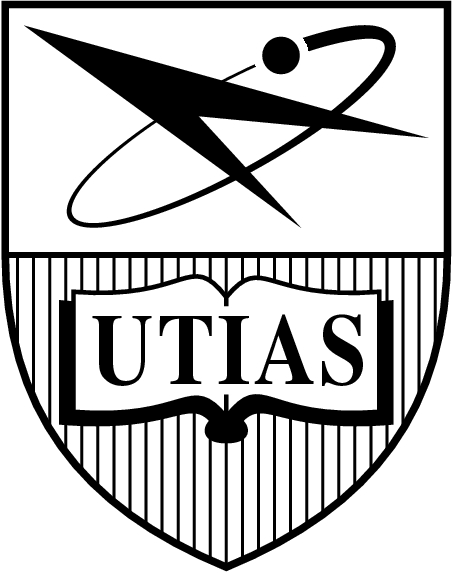
\includegraphics[width=0.2\textwidth]{Figs/utias-logo-black.png} \par}
\end{lrbox}

% Author Box
\newsavebox{\titlepgauthor}
\begin{lrbox}{\titlepgauthor}
  \begin{minipage}[c]{\textwidth}
    \centering \Large \bfseries{Anton Rubisov}
  \end{minipage}
\end{lrbox}

% Department Box
\newsavebox{\titlepgdept}
\begin{lrbox}{\titlepgdept}
  \begin{minipage}[c]{\textwidth}
    \centering       
      {\large University of Toronto Institute for Aerospace Studies \par}
      {\large Faculty of Applied Science and Engineering  \par}
	  {\large University of Toronto \par}
  \end{minipage}
\end{lrbox}

% Submission Box
\newsavebox{\titlepgsubmission}
\begin{lrbox}{\titlepgsubmission}
  \begin{minipage}[c]{\textwidth}
    \begin{center}
      \large A thesis submitted in partial fulfilment for the degree of \par
      \large \textit{Master of Applied Science} \par
    \end{center}
  \end{minipage}
\end{lrbox}

% College and Date Box
\newsavebox{\titlepggraddate}
\begin{lrbox}{\titlepggraddate}
\begin{minipage}[c]{0.95\textwidth}
  \large October 2015
\end{minipage}
\end{lrbox}

%  Now to compute the free vertical space
\newlength{\titlepgspacing}
\setlength{\titlepgspacing}{ \textheight %
			- \totalheightof{\usebox{\titlepgtitle}}
			- \totalheightof{\usebox{\titlepgcrest}}
			- \totalheightof{\usebox{\titlepgauthor}}
			- \totalheightof{\usebox{\titlepgdept}}
			- \totalheightof{\usebox{\titlepgsubmission}}
			- \totalheightof{\usebox{\titlepggraddate}}
}
}

\renewcommand{\maketitle}{

% To compute the free vertical space in Title page
\computeTitlePageSpacing

\begin{singlespace}
\begin{center}

% Title
\vspace*{.1\titlepgspacing}
{\usebox{\titlepgtitle}} % subtitle is defined

% Crest
\vspace{.15\titlepgspacing}
{\usebox{\titlepgcrest}}
\vspace{.15\titlepgspacing}

% Author
{\usebox{\titlepgauthor}}
\vspace*{1em}

% Department and University
{\usebox{\titlepgdept}}
\vspace{.2\titlepgspacing}

% Submission Text
{\usebox{\titlepgsubmission}}

\end{center}

% College and degree date
\vfill
{\usebox{\titlepggraddate}}
\end{singlespace}
}

\maketitle
% ************************** Thesis Abstract *****************************
\vspace*{0.25in}

\begin{center}
	{\Large\bf Statistical Arbitrage with \\ Limit Order Book Imbalance \par}
	{\large Anton Rubisov \par}
	{University of Toronto Institute for Aerospace Studies}\\
    {Faculty of Applied Science and Engineering}\\
	{University of Toronto \par}
	{2015}
\end{center}
\vspace{0.25in}	
{\Large\bf Abstract}
\vspace{0.25in}

\begin{quote}
This dissertation demonstrates that there is high revenue potential in using limit order book imbalance as a state variable in an algorithmic trading strategy. Beginning with the hypothesis that imbalance of bid/ask order volumes is an indicator for future price changes, exploratory data analysis suggests that modelling the joint distribution of imbalance and observed price changes as a continuous-time Markov chain presents a monetizable opportunity. The arbitrage problem is then formalized mathematically as a stochastic optimal control problem using limit orders and market orders with the aim of maximizing terminal wealth. The problem is solved in both continuous and discrete time using the dynamic programming principle, which produces both conditions for market order execution, as well as limit order posting depths, as functions of time, inventory, and imbalance. The optimal controls are calibrated and backtested on historical NASDAQ ITCH data, which produces consistent and substantial revenue.
\end{quote}
% ************************** Thesis Acknowledgements **************************
\newenvironment{acknowledgements}%
	{\cleardoublepage\thispagestyle{empty}%
	\chapter*{\centering \Large Acknowledgements}}%
	
	\begin{acknowledgements}
I couldn't begin to enumerate the times and ways this dissertation could have failed to be. I am deeply grateful to several individuals for making it a reality, and I'd like to acknowledge them here.

\href{http://www.sr.utias.utoronto.ca/}{\bf Dr. Gabriele D'Eleuterio}, my supervisor at UTIAS, is the epitomical supernatural mentor of the hero journey, without whom I would have abandoned my studies. Gabe was the inspirational upholder of academic values, who relentlessly stressed the subtleties of scientific presentation and communication, and guided me through a pretty tough time. Thank you for your support, guidance, and for every coffee.

\href{http://www.utstat.utoronto.ca/sjaimung/}{\bf Dr. Sebastian Jaimungal}, professor of statistics at the university, took me on as a surrogate student half-way through my studies, and guided every step of this dissertation. Despite having absolutely no obligation to do so, he had faith in me and patience with me in navigating an entirely unfamiliar subject. Thank you for repeatedly making yourself available to help with all the math.

\href{http://jackcarlyle.co.uk/}{\bf Dr. Jack Carlyle}, then a PhD student in solar physics at UCL, inspired me to quit my job and go back to school for a graduate degree. It wasn't an easy decision, and the jury is out on whether it was a good one. But thanks for all the tea and crumpets.

\href{https://www.linkedin.com/in/tedherman}{\bf Ted Herman}, a friend that redefines friendship, has read more of my research than anyone ever will. At a crucial time, we struck the \href{http://www.fransrestaurant.com/home}{Fran's} Accord that involved prewritten \$100 cheques being shredded on a weekly basis upon receipt of a progress update. Legitimately, this is probably the number one reason that my dissertation got done.

Thank you {\bf mom} for always loving, supporting, and inspiring me to my best. Thank you {\bf dad} for pretty well being a supervisor too.
	\end{acknowledgements}

% *********************** Adding TOC and List of Figures ***********************
\tableofcontents
\listoffigures
\listoftables

% ******************************** Main Matter *********************************
\chapter{Introduction}

With the introduction of mathematical models, participation in financial markets evolved from an art to a science. Beginning with Harry Markowitz's modern portfolio theory, moving through the capital asset pricing model and the Black-Scholes option pricing model, modern finance is now replete with models for pricing derivatives, credit scores, and costs of capital; what was once speculation is now calculation. Crucially, models lead to algorithms, which remove human error and add the ability to process large sets of data. 

The process of running computer algorithms to execute orders on an electronic exchange such as NASDAQ is known as \emph{algorithmic trading}. Speed of execution is typically crucial, often requiring running the algorithms on servers directly wired to the exchange, known as \emph{co-location}. Closely related is \emph{high-frequency trading}, which refers simply to the timescale, generally milliseconds, on which the algorithms submit orders. In theory, high-frequency trading is encompassed by algorithmic trading, while not all algorithmic trading need be high-frequency; in practice, the two terms are often used interchangeably. 

The particular algorithms used in algorthmic trading vary greatly across the different types of strategies employed. Non-revenue-generating algorithmic trading is generally aimed at transaction cost reduction, with the primary theoretical paper on the subject being \citet{Bertsimas98} and \citet{Almgren01}. When an institutional investor wishes to buy or sell a large quantity of shares, the aim of the trader is to obtain the best possible price compared with some benchmark (often taken to be the midprice at the time of initiating the strategy). Here the definition of `large' is determined relative to the liquidity of the stock - either in comparison to the average size of trades for the given stock, or to the available quantity to be bought/sold at the best listed price. The goal of the algorithmic trading strategy is then to split the large order into smaller pieces and execute them on an algorithmically-determined schedule, balancing the total time for execution with the volatility of the price the trader will receive. 

Conversely, an example of algorithmic trading that capitalises on arbitrage opportunities to generate revenue is cross-exchange arbitrage, which uses simple, low-latency algorithms to profit from price discrepancies of a single stock dual-listed on two exchanges. The server running the algorithm is co-located at one of the exchanges, algorithm latency is on the order of microseconds, and the limiting reagent is the time taken for information to travel to and from the other exchange. In the case of Chicago and New York, for example, information can make the trip in 6ms via optical fibres that send information at about half the speed of light. For this reason, agents are now paying for access to a system of ground satellites that has been set up to relay information between the two exchanges via microwaves, shaving latency down to 4ms \citep{Laughlin14}. Another class of strategies for generating revenue using algorithmic trading are statistical arbitrage strategies, which use complex algorithms to profit from observed statistical patterns of a single stock on a single exchange. In statistical arbitrage, the aim is to exploit predictable statistical patterns in the available data provided by the exchange, such as predicting stock price movements from prices observed thus far. This method too requires co-location, and operates on the scale of milliseconds. It is this type of high-frequency trading that is explored in this dissertation. 

As part of the Dodd-Frank Act of 2010, the Volcker Rule has banned US banks from making certain speculative investments, and in so doing effectively curbed their proprietary high frequency trading activity. Nevertheless, as they are still required to provide liquidity to markets via market-making (offering to both buy and sell financial instruments), banks use algorithmic trading to determine the bid/ask bands they will send to exchanges. Exploiting arbitrage opportunities using high frequency trading remains unrestricted for hedge funds, and notably has been used by Renaissance Technologies LLC's flagship Medallion fund to generate an average 71.8 percent annual return, before fees, from 1994 through mid-2014 \citep{rentech}. However, as it remains exclusive to only Renaissance employees and family members, it serves instead as a reminder of the revenue potential of high frequency algorithmic trading.

\section{The Limit Order Book}

A \emph{limit order} is an instruction submitted by an agent to buy or sell up to a specified quantity or volume of a financial instrument, and at a specified price. A \emph{limit order book (LOB)} is the accumulated list of such orders sent to a given exchange, where each order is accompanied by a timestamp and an anonymous key that uniquely identifies the agent. The exchange runs a trade matching engine that uses the LOB to pair buy and sell requests that concur on price, even if only partially on volume. Orders remain in effect until they are modified, cancelled, or fully filled \citep{Kyle1989}.

The unfilled or partially filled orders accumulate in the limit order book and provide liquidity to the market. At any given time, the structure of the LOB can be visualised as in \autoref{fig:LOB}. As new limit orders arrive, they are compared with existing opposing orders in the book in search of a match - and if so, existing orders are \emph{filled} or \emph{lifted} according to a first-in-first-out priority queue for each price level. The price levels can also be referred to by their \emph{depth}, where the best bid and ask prices are called \emph{at-the-touch} and have a depth of zero, and depth increases in either direction according to the absolute price difference from the at-the-touch depths; the buy limit order at \$28.92 is at a depth of \$0.02. \emph{Market orders} extend the idea of limit orders by specifying only the volume, and accept the best possible price currently available in the LOB; whereas limit orders are free to post, modify, and cancel (as an incentive for providing liquidity), a fee is charged for executing a market order.

\begin{figure}
  \tikzsetnextfilename{Ch1/LOB}
  %\documentclass{article}
%\usepackage{pgfplots}
%\usetikzlibrary{backgrounds}
%\begin{document}
% Limit Order Book structure and mechanics by Anton, inspired by Ash Booth
\pgfdeclarepatternformonly[\LineSpace]{myhatch}{\pgfqpoint{-1pt}{-1pt}}{\pgfqpoint{\LineSpace}{\LineSpace}}{\pgfqpoint{\LineSpace}{\LineSpace}}%
{
    \pgfsetlinewidth{1pt}
    \pgfpathmoveto{\pgfqpoint{0pt}{\LineSpace}}
    \pgfpathlineto{\pgfqpoint{\LineSpace + 0.1pt}{-0.1pt}}
    \pgfusepath{stroke}
}

\newdimen\LineSpace
\tikzset{
    line space/.code={\LineSpace=#1},
    line space=5pt
}

\colorlet{buyLOcolor}{black!25}%
\colorlet{sellLOcolor}{black!90}%
\begin{center}%
\makebox[0pt]{%
\begin{tikzpicture}[
	/pgf/number format/fixed,
	/pgf/number format/fixed zerofill,	
	/pgf/number format/precision=2,
	buyLOone/.style ={rectangle,draw=black, fill=buyLOcolor,thick,outer sep = 0.05cm,minimum size=0.9cm,anchor=south,rounded corners=0.2cm},
	buyLOonematch/.style ={rectangle,draw=black,thick,outer sep=0.05cm,minimum size=0.9cm,anchor=south,rounded corners=0.2cm,preaction={fill=buyLOcolor},pattern=myhatch},
	buyLOtwo/.style ={rectangle,draw=black, fill=buyLOcolor,thick,outer sep = 0.05cm,minimum height =1.9cm ,minimum width=0.9cm,anchor=south,rounded corners=0.2cm},
	buyLOthree/.style ={rectangle,draw=black, fill=buyLOcolor,thick,outer sep = 0.05cm,minimum height=2.9cm,minimum width=0.9cm,anchor=south,rounded corners=0.2cm},
	sellLOone/.style ={rectangle,draw=black, fill=sellLOcolor,thick,outer sep = 0.05cm,minimum size=0.9cm,anchor=south,rounded corners=0.2cm},
	sellLOtwo/.style ={rectangle,draw=black, fill=sellLOcolor,thick,outer sep = 0.05cm,minimum height=1.9cm ,minimum width=0.9cm,anchor=south,rounded corners=0.2cm},
	sellLOthree/.style ={rectangle,draw=black, fill=sellLOcolor,thick,outer sep = 0.05cm,minimum height=2.9cm,minimum width=0.9cm,anchor=south,rounded corners=0.2cm}]
    \draw [>=latex,->] (-0.55,-0.05) -- (12,-0.05) node[draw=none,fill=none,midway,shift=(down:1),font=\Large] {Price};
    \draw [>=latex,->] (-0.55,-0.05) -- (-0.55,9) node[draw=none,fill=none,midway,rotate=90,shift=(up:0.75),font=\Large] {Volume};
    
    \foreach \x [evaluate=\x as \price using \x/100 + 28.90]  in {0,...,11} \draw (\x ,-0.05) -- (\x ,-0.1) node[anchor=north] {$\scriptstyle\pgfmathprintnumber{\price}$};

%%% LOB
	\node[buyLOone]			at (0,0) {};
	\node[buyLOone]			at (0,1) {};
	\node[buyLOtwo]			at (1,0) {};
	\node[buyLOone]			at (1,2) {};
	\node[buyLOthree]		at (2,0) {};
	\node[buyLOtwo]			at (3,0) {};
	\node[buyLOtwo]			at (3,2) {};
	\node[buyLOtwo]			at (3,4) {};
	\node[buyLOonematch]	at (4,0) {};
	\node[buyLOonematch]	at (4,1) {};
	\node[buyLOtwo] 		at (4,2) {};
	\node[buyLOone] 		at (4,4) {};
	
	\node[sellLOone]			at (7,0) {};
	\node[sellLOone]			at (7,1) {};
	\node[sellLOone]			at (7,2) {};
	\node[sellLOtwo]			at (8,0) {};
	\node[sellLOtwo]			at (10,0) {};
	\node[sellLOthree]		at (11,0) {};
	\node[sellLOthree]		at (11,3) {};

%%% BID ASK SPREAD
	\draw [<->] (5,1.5)  -- (6,1.5) node[midway, anchor=north, text width=2cm, align=center, thick] {Bid-Ask \\ Spread};

%%% MARKET ORDER		
	\node[sellLOtwo]			at (4,7) {};
	\draw[->, ultra thick] (4,7) -- (4,0.5);
	\node at (3.5,9) [anchor=north east, text width=3cm, align=right, font=\tiny] {A market order to sell two shares arrives, and matches with the first two limit orders in the queue at the best price.};
	
%%% LIMIT ORDER
	\node[sellLOone]			at (7,5) {};
	\draw[->, ultra thick] (7,5) -- (7,3);
	\node at (7.5,6) [anchor=north west, text width=2cm, align=left, font=\tiny] {A limit order to sell one share at 28.97 arrives, and is added to the back of the queue.};	
	
%%% LEGEND
	\node[buyLOone]			at (8,8) {};
	\node[sellLOone]			at (8,7) {};
	\node at (8.5,8.5) [anchor=west, align=left] {Bid (buy) LO};
	\node at (8.5,7.5) [anchor=west, align=left] {Ask (sell) LO};
\end{tikzpicture}
}
\end{center}
%\end{document}

%  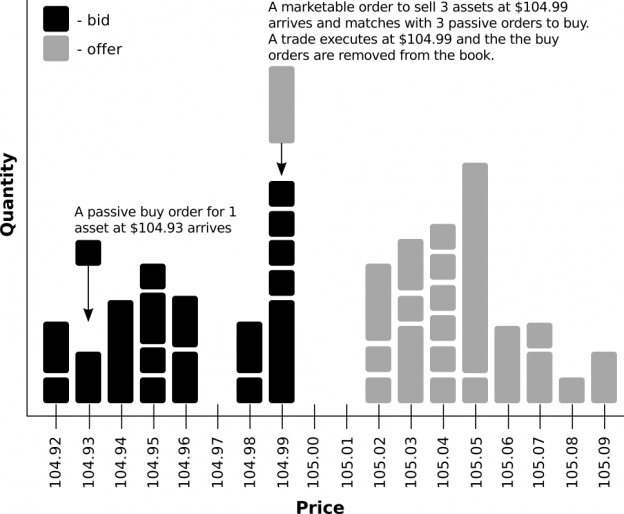
\includegraphics[width=0.9\textwidth]{Figs/LOBAshBooth.png}
\caption[Structure and mechanics of the limit order book]{Structure and mechanics of the limit order book, adapted from \citet{Booth15}. Each block represents an order, of varying volumes, submitted by various agents participating in the market.}
\label{fig:LOB}
\end{figure}

In the literature, LOBs are generally modelled in one of two ways: either by an economics-based approach, or a physics-based approach \citep{Summary2013}. The economics-based approaches are trader-centric, assume perfect rationality, view order flow as static, and seek to understand trader strategies, in particular through game-style theories. By contrast, the physics-based approach, with which we are more concerned here, assumes zero-intelligence, provides conceptual toy models of the evolution of the book, and is concerned with the search for statistical regularity. The dynamics of the book, namely order arrivals and cancellations, are governed by stochastic processes of varying complexity, from particles on a 1-D price lattice \citep{Bak97} to independent Poisson processes governing the arrival, modification, and cancellation of orders \citep{Cont10}. An excellent literature survey on LOB modelling can be found in \citet{Summary2013}.

\section{ITCH Data Set}
The underlying data that will be used in this work to generate imbalance and price change timeseries comes from the NASDAQ Historical TotalView-ITCH. ITCH\footnote{Remarkably, according to a representative of the NASDAQ, `ITCH' does not stand for anything.} is a  direct data-feed protocol that makes it possible for those with a paid subscription to track the status of every order from arrival until cancellation or execution. The Historical TotalView is simply a historical record of the events in the live feed. In the data used in this work, timestamps are provided to 1 millisecond, though newer versions of the feed offer nanosecond precision. Our data has been converted to MATLAB format; below, the structure of the event feed is described in detail (retaining only relevant fields):

\begin{table}[H]
\centering
\ra{1.2}
\begin{tabular}{@{} *{5}{c} @{}}
\toprule
Time & Order ID & Event & Volume & Price \\
\midrule
\vdots & \vdots & \vdots & \vdots & \vdots \\
39960699 &72408630 & 66 & 100 & 1107000 \\
39960710 & 72408630 & 68 & 100 & 1107000 \\
\vdots & \vdots & \vdots & \vdots & \vdots \\
\bottomrule
\end{tabular}
\label{tbl:ITCHevents}
\end{table}
{\bf Time:} Order arrival time in milliseconds from midnight. \\
{\bf Order ID:} Unique order reference number. \\
{\bf Event:} Event type:
\vspace{-\topsep}
\begin{itemize}[label={},nolistsep]
\item 66 -- Add buy order
\item 83 -- Add sell order
\item 69 -- Execute outstanding order in part
\item 67 -- Cancel outstanding order in part
\item 70 -- Execute outstanding order in full
\item 68 -- Delete outstanding order in full
\item 88 -- Bulk volume for the cross event
\item 84 -- Execute non-displayed order
\end{itemize}
\vspace{-\topsep}
{\bf Volume:} Number of shares. \\
{\bf Price:} Dollar price times 10,000. \par  
Thus, in the above example, we have a buy order arriving at 11:06am for 100 shares at \$100.70, and being cancelled 11 milliseconds later. From this feed we are able to reconstruct the entire limit order book at any point in time, which amounts to being able to generate a plot as in \autoref{fig:LOB} detailing the exact liquidity available at each order depth.

\section{Order Imbalance}

A core component of this dissertation is limit order book imbalance. \emph{Imbalance} is a ratio of limit order volumes between the bid and ask side, and in the work that follows is calculated as 
\begin{equation}\label{eq:LOBImbalance}
I(t) = \dfrac{V_{bid}(t) - V_{ask}(t)}{V_{bid}(t) + V_{ask}(t)} \in [-1,1]
\end{equation}
where both $V_{bid}$ and $V_{ask}$ are computed as the weighted average volumes at the three lowest depths having non-zero volume, using exponentially decreasing weights. As a sample calculation, the imbalance of the sample LOB presented in \autoref{fig:LOB} (prior to order arrivals) would be
\begin{align*}
V_{bid} & = \text{weight}(28.94)\cdot\text{volume}(28.94) \\
& \hphantom{{}={}} + \text{weight}(28.93)\cdot\text{volume}(28.93) \\
& \hphantom{{}={}} + \text{weight}(28.92)\cdot\text{volume}(28.92) \\
& = e^{-0.5 (0)} \cdot 5 + e^{-0.5 (1)} \cdot 6 + e^{-0.5 (2)} \cdot 3\\
& = 1.0000 \cdot 5 + 0.6065 \cdot 6 + 0.3679 \cdot 3 \\
& = 9.7428 \\
V_{ask} & = 4.9488 \\
I(t) & = \dfrac{9.7428 - 4.9488}{9.7428 + 4.9488} \\
&  = 0.3263
\end{align*}
In the figure we see that there are more limit orders on the bid side than on the ask, and the above value confirms that there is a medium imbalance in favour of the bid side.

\section{Roadmap}
The remainder of this dissertation is structured as follows:

{\bf Chapter 2} explores the possibility of constructing naive trading strategies using the statistical properties arising from modelling imbalance as a continuous time Markov chain; a basic understanding of probability theory is required. 

{\bf Chapter 3} casts the same statistical arbitrage problem into a stochastic optimal control framework, and solves it in both continuous and discrete time; familiarity with stochastic calculus and dynamic programming is assumed. 

{\bf Chapter 4} presents calibrations of the optimal controls and explores their dynamics. In-sample and out-of-sample backtests are conducted on historical ITCH data, which show a 652\% ROI over 2014.

{\bf Chapter 5} concludes the dissertation by restating the primary backtesting results in the context of operational costs, and summarizes the key assumptions and simplifications that have been made. The conclusions are intended as considerations for future work on this topic.
\chapter{Exploratory Data Analysis}

\section{Modelling Imbalance: Continuous Time Markov Chain}
The aim of this research project is to utilize the LOB volume imbalance $I(t)$ in an algorithmic trading application; hence, a suitable choice of model for $I(t)$ must be made. Rather than modelling imbalance directly as a real-valued process, an alternative approach, and that which is utilized herein, is to discretize the imbalance value $I(t)$ into subintervals, or bins, and fit the resulting process to a continuous-time Markov chain.

The following definitions and properties are adapted from \cite{STAT455}:
\begin{defn}
A continuous-time stochastic process $\left\lbrace X(t) \; | \; t \geq 0 \right\rbrace$ with state space $S$ is called a \emph{continuous-time Markov chain (CTMC)} if it has the Markov property; namely, that 
\begin{equation}
\P \left[ X(t) = j \; | \; X(s) = i, X(t_{n-1} = i_{n-1}, \dots , X(t_1) = i_1 \right] = \P \left[ X(t) = j \; | \; X(s) = i \right]
\end{equation}
where for any integer $n \geq 1$, $0 \leq t_1 \leq \dots \leq t_{n-1} \leq s \leq t$ is any non-decreasing sequence of $n+1$ times, and $i_1,\dots,i_{n-1}, i, j \in S$ are any $n+1$ states.
\end{defn}
\begin{defn} A CTMC $X(t)$ is \emph{time homogeneous} if for any $s \leq t$ and any states $i,j \in S$,
\begin{equation}
\P \left[ X(t) = j \; | \; X(s) = i \right] = \P \left[ X(t-s) = j \; | \; X(0) = i \right]
\end{equation}
\end{defn}
\begin{defn}
The key quantities that determine a CTMC $X(t)$ are the \emph{transition rates} $q_{ij}$, which specify the rate at which $X$ jumps from state $i$ to $j$. Conditional on leaving state $i$, $X$ transitions to state $j$ with \emph{conditional transition probability} $p_{ij}$. The amount of time that $X$ spends in state $i$, called the \emph{holding time}, is exponentially distributed with rate $v_i$. These quantities are related by:
\begin{align}
v_i & = \sum_{\substack{j \in S \\ j \neq i}} q_{ij} \\
q_{ij} & = v_i \cdot p_{ij} \\
p_{ij} & = \frac{q_{ij}}{v_i}
\end{align} 
\end{defn}
\begin{defn}
A CTMC $X(t)$ has an \emph{infinitesimal generator matrix} $\mat{G}$, whose entries are
\begin{align}
g_{ij} &= q_{ij}, \qquad i \neq j \\
g_{ii} & = -v_i
\end{align}
If $X(t)$ has transition probabilities $P_{ij}(t) = \P \left[ X(t) = j \; | \; X(0) = i \right]$ and matrix $\mat{P}(t) = \lbrace P_{ij}(t) \rbrace$, then $\mat{P}(t)$ and $\mat{G}$ are related by
\begin{align}
\dot{\mat{P}}(t) & = \mat{G} \cdot \mat{P}(t) \\
\mat{P}(t)  &= e^{\mat{G}t} \label{eq:CTMCPG}
\end{align}
\end{defn}

Conditional on $Z(t) = k$, we assume the arrival of buy and sell market orders follow independent Poisson processes with intensities $\lambda_k^\pm$, where $\lambda_k^+$ ($\lambda_k^-$) is the rate of arrivals of market buys (resp. sells). Such processes are called \textit{Markov-modulated Poisson processes}, as the Poisson intensities are themselves stochastic processes determined by the state of the Markov chain. Thus, a timeline of observations of arrivals of buy/sell market orders and of regime switches might look like:
\begin{figure}
  \tikzsetnextfilename{LOBtimeline}
  % Limit Order Book timeline by Anton
%

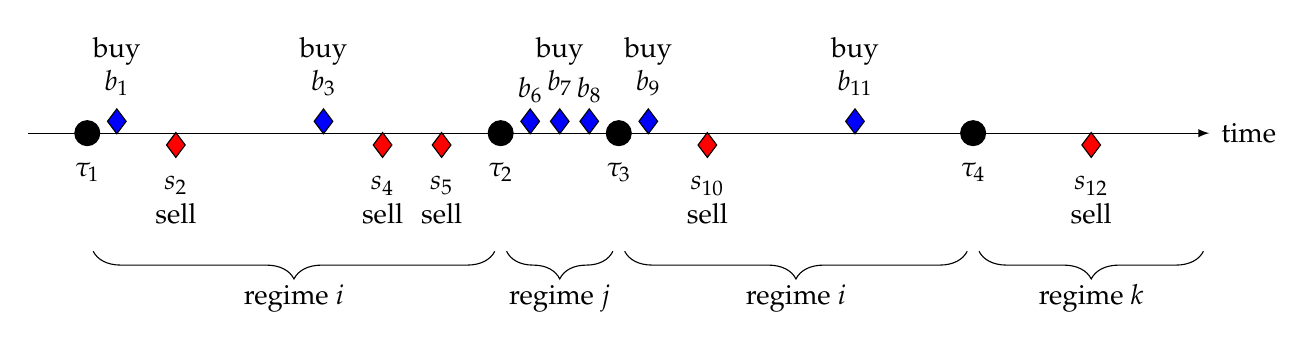
\begin{tikzpicture}[scale=1.5]
	[triangle/.style = {fill=blue!20, regular polygon, regular polygon sides=3 },
	border rotated/.style = {shape border rotate=180}]
	
    \draw [>=latex,->] (0,0) -- (10,0) node[draw=none,fill=none,shift=(right:0.5)] {time};
    \draw[mark options={fill=black}, mark size=+3pt] plot[mark=*] coordinates {(.5,0)} node[shift=(down:0.5), align=center] {$\tau_1$};
    \draw[mark options={fill=black}, mark size=+3pt] plot[mark=*] coordinates {(4,0)} node[shift=(down:0.5), align=center] {$\tau_2$};
    \draw[mark options={fill=black}, mark size=+3pt] plot[mark=*] coordinates {(5,0)} node[shift=(down:0.5), align=center] {$\tau_3$};
    \draw[mark options={fill=black}, mark size=+3pt] plot[mark=*] coordinates {(8,0)} node[shift=(down:0.5), align=center] {$\tau_4$};
    
    
	\draw[mark options={fill=blue}, mark size =+3pt, shift=(up:0.1)] plot[mark=diamond*] coordinates {(.75,0)} node[shift=(up:0.7), align=center] {buy \\ $b_1$};
	\draw[mark options={fill=red}, mark size =+3pt, shift=(down:0.1)] plot[mark=diamond*] coordinates {(1.25,0)} node[shift=(down:0.7), align=center] {$s_2$ \\ sell};
	\draw[mark options={fill=blue}, mark size =+3pt, shift=(up:0.1)] plot[mark=diamond*] coordinates {(2.5,0)} node[shift=(up:0.7), align=center] {buy \\ $b_3$};
	\draw[mark options={fill=red}, mark size =+3pt, shift=(down:0.1)] plot[mark=diamond*] coordinates {(3,0)} node[shift=(down:0.7), align=center] {$s_4$ \\ sell};
	\draw[mark options={fill=red}, mark size =+3pt, shift=(down:0.1)] plot[mark=diamond*] coordinates {(3.5,0)} node[shift=(down:0.7), align=center] {$s_5$ \\ sell};

%%% REGIME SWITCH
	
	\draw[mark options={fill=blue}, mark size =+3pt, shift=(up:0.1)] plot[mark=diamond*] coordinates {(4.25,0)} node[shift=(up:0.4), align=center] {$b_6$};
	\draw[mark options={fill=blue}, mark size =+3pt, shift=(up:0.1)] plot[mark=diamond*] coordinates {(4.50,0)} node[shift=(up:0.7), align=center]
{buy \\ $b_7$};
	\draw[mark options={fill=blue}, mark size =+3pt, shift=(up:0.1)] plot[mark=diamond*] coordinates {(4.75,0)} node[shift=(up:0.4), align=center] {$b_8$};
	
%%% REGIME SWITCH

	\draw[mark options={fill=blue}, mark size =+3pt, shift=(up:0.1)] plot[mark=diamond*] coordinates {(5.25,0)} node[shift=(up:0.7), align=center] {buy \\ $b_9$};
	\draw[mark options={fill=red}, mark size =+3pt, shift=(down:0.1)] plot[mark=diamond*] coordinates {(5.75,0)} node[shift=(down:0.7), align=center] {$s_{10}$ \\ sell};
	\draw[mark options={fill=blue}, mark size =+3pt, shift=(up:0.1)] plot[mark=diamond*] coordinates {(7,0)} node[shift=(up:0.7), align=center] {buy \\ $b_{11}$};
	
%%% REGIME SWITCH

	\draw[mark options={fill=red}, mark size =+3pt, shift=(down:0.1)] plot[mark=diamond*] coordinates {(9,0)} node[shift=(down:0.7), align=center] {$s_{12}$ \\ sell};
	
%%% BRACES
	
	\draw [decorate, decoration = {brace, amplitude = 10pt, mirror}]
	(0.55,-1) -- (3.95,-1) node [black, midway, yshift = -0.6cm] {regime $i$};
	\draw [decorate, decoration = {brace, amplitude = 10pt, mirror}]
	(4.05,-1) -- (4.95,-1) node [black, midway, yshift = -0.6cm] {regime $j$}; 
	\draw [decorate, decoration = {brace, amplitude = 10pt, mirror}]
	(5.05,-1) -- (7.95,-1) node [black, midway, yshift = -0.6cm] {regime $i$}; 
	\draw [decorate, decoration = {brace, amplitude = 10pt, mirror}]
	(8.05,-1) -- (9.95,-1) node [black, midway, yshift = -0.6cm] {regime $k$}; 
\end{tikzpicture}

\caption{Hypothetical timeline of market orders arriving during changing order imbalance regimes.}
\label{introtimeline}
\end{figure}

In the sections that follow, I derive maximum likelihood estimations for the parameters of the CTMC, and evaluate the fit of the model to the data.

\section{Maximum Likelihood Estimate of a Markov-modulated Poisson Process}

\subsection{Maximum Likelihood Estimation of \texorpdfstring{$G$}{G}}

Let $\mat{G}$ be the generator matrix for a CTMC $Z(t)$ with state space $K$. From observations, e.g. the fictional events in the timeline given in Figure \ref{introtimeline}, we want to estimate the entries of $\mat{G}$. Since the holding time in a given state $i$ has pdf $f(t;v_i) = v_i e^{-v_i t}$, the likelihood function (allowing for repetition of terms) would therefore be:
\begin{align}
\mathcal{L}(\mat{G}) &= (v_{i} e^{-v_{i}(\tau_2 - \tau_1)} p_{ij}) (v_{j} e^{-v_{j}(\tau_3 - \tau_2)} p_{ji}) (v_{i} e^{-v_{i}(\tau_4 - \tau_3)} p_{ik}) \dots \\
&= \prod\limits_{i=1}^{K} \prod\limits_{i \neq j} (v_{i}p_{ij})^{N_{ij}(T)} e^{-v_{i}H_i(T)} \\
&= \prod\limits_{i=1}^{K} \prod\limits_{i \neq j} (q_{ij})^{N_{ij}(T)} e^{-v_{i}H_i(T)}
\intertext{where:}
N_{ij}(T) & \equiv \mbox{number of transitions from regime $i$ to $j$ up to time $T$} \nonumber \\
H_{i}(T) & \equiv \mbox{holding time in regime $i$ up to time $T$} \nonumber
\intertext{So that the log-likelihood becomes:} 
\ln \mathcal{L}(\mat{G}) & = \sum\limits_{i=1}^{K} \sum\limits_{i \neq j} \left[ N_{ij}(T) \ln(q_{ij}) - v_{i} H_i(T) \right] \\
&= \sum\limits_{i=1}^{K} \sum\limits_{i \neq j} \left[ N_{ij}(T) \ln(q_{ij}) - \left( \sum\limits_{i \neq k} q_{ik} H_i(T) \right) \right]
\end{align}
To get a maximum likelihood estimate $\hat{q}_{ij}$ for transition rates and therefore the matrix $\mat{G}$, we take the partial derivative of $\ln \mathcal{L}(\mat{G})$ and set it equal to zero:
\begin{equation}
\dfrac{\partial \ln \mathcal{L}(\mat{G})}{\partial q_{ij}} = \dfrac{N_{ij}(T)}{q_{ij}} - H_i(T) = 0
\end{equation}
\begin{equation}\label{eq:MLEG}
\Rightarrow \hat{q}_{ij} = \dfrac{N_{ij}(T)}{H_i(T)}
\end{equation}

\subsection{Maximum Likelihood Estimation of \texorpdfstring{$\lambda^{\pm}_k$}{lpmk}}

Now we want to derive an estimate for the intensity of the Poisson process of market order arrivals conditional on being in state $k$. We'll look first at just the buy market orders for some regime $k$, as the sell case is identical. Let the buy market order arrival times be indexed by $b_i$. Since we're assuming that the arrival process is Poisson with the same intensity throughout trials, we can consider the inter-arrival time of events conditional on being in state $k$. Then the MLE derivation follows just as for the generator matrix:
\begin{align}
\mathcal{L}(\lambda^{+}_k ; b_1, \dots, b_N) &= \prod\limits_{i=2}^{N} \lambda^{+}_k e^{-\lambda^{+}_k (b_{i} - b_{i-1})} \\
&= (\lambda^{+}_k)^{N^{+}_k(T)} e^{-\lambda^{+}_k H_k(T)}
\intertext{where:}
N^{+}_{k}(T) & \equiv \mbox{number of market order arrivals in regime $k$ up to time $T$} \nonumber \\
H_{k}(T) & \equiv \mbox{holding time in regime $k$ up to time $T$} \nonumber
\intertext{So that the log-likelihood becomes:} 
\ln \mathcal{L}(\lambda^{+}_k) & = N^{+}_k(T) \ln(\lambda^{+}_k) -\lambda^{+}_k H_k(T)
\intertext{And the ML estimate for $\hat{\lambda}^{+}_k$ is:} 
\dfrac{\partial \ln\mathcal{L} }{\partial \lambda^{+}_k} & = 
\dfrac{N^{+}_k(T)}{\lambda^{+}_k} - H_k(T) = 0
\end{align}
\begin{equation}\label{eq:MLElambda}
\Rightarrow \hat{\lambda}^{+}_k = \dfrac{N^{+}_k(T)}{H_k(T)}
\end{equation}

\section{2-Dimensional CTMC}
\label{sec:2DCTMC}
Next we consider a CTMC that jointly models the imbalance bin and the price change over a subsequent interval. That is, the CTMC models the joint distribution $(I(t), \Delta S(t))$ where $I(t) \in \lbrace 1,2,\dots,\#_{bins} \rbrace$ is the bin corresponding to imbalance averaged over the interval $[t-\Delta t_I, t]$, and $\Delta S(t) = \sgn(S(t+\Delta t_S)-S(t)) \in \lbrace -1, 0, 1 \rbrace$.  The pair $(I(t), \Delta S(t))$ is then reduced into one dimension with a simple encoding which we will denote $\varphi(I(t),S(t))$; for example, using 3 bins:

\begin{table}[H]
\centering
\ra{1.2}
\begin{tabular}{@{}rrrcrrrcrrr@{}}
\toprule
$Z(t)$ & Bin $I(t)$ & $\Delta S(t)$ & \phantom{abc} & $Z(t)$ & Bin $I(t)$ & $\Delta S(t)$ & \phantom{abc} & $Z(t)$ & Bin $I(t)$ & $\Delta S(t)$ \\
\cmidrule{1-3} \cmidrule{5-7} \cmidrule{9-11}
1 & Bin 1 & $<0$ && 4 & Bin 1 & $0$ && 7 & Bin 1 & $>0$ \\
2 & Bin 2 & $<0$ && 5 & Bin 2 & $0$ && 8 & Bin 2 & $>0$ \\
3 & Bin 3 & $<0$ && 6 & Bin 3 & $0$ && 9 & Bin 3 & $>0$ \\
\bottomrule
\end{tabular}
\caption{$\varphi(I(t),S(t))$: 1-Dimensional Encoding of 2-Dimensional CTMC}
\end{table}

\subsection{Cross-Validation}
We cross-validate the CTMC calibration by means of a time-homogeneity test similar to that done in \cite{Tan02}. The null hypothesis is given by \cite{Weiss10}:
\begin{equation}
H_0 = \forall i,j \in S \; : \; \exists q_{ij} \in \R^+ \; : \; q_{ij}(t) \equiv q_{ij} \forall t \in [0,T]
\end{equation}
whereas the alternative hypothesis states that transition rates/probabilities are time-dependent. To test the hypothesis, we fix an imbalance averaging time $\Delta t_I$, number of imbalance bins, and calculate the MLE estimate of the infinitesimal generator matrix $\mat{G}$ on the full timeseries. For a chosen error threshold $\epsilon$, we use the relationship in \eqref{eq:CTMCPG} to calculate the number of timesteps $n_{conv}$ of size $\Delta t_I$ such that
\begin{equation}\label{eq:crossvalidnconv}
|| \mat{P}\left((n_{conv}+1)\Delta t_I \right) - \mat{P} \left( n_{conv}\Delta t_I \right) || < \epsilon
\end{equation}
This value $n_{conv}$ determines the size of the cross-validation timewindow into which to partition the full timeseries, yielding $K$ equal subintervals of length $n$. For comparison, we also partitioned the timeseries into 8, 4, and 2 equal intervals. For each ``removed series'' $k \in \{ 1,\dots,K \}$, we recalibrate a CTMC generator matrix $\mat{G}_{k}$. Finally, we test whether the one-step transition probabilities $p_{ij}^k$ contained in $\mat{P}_k \left(\Delta t_I \right)$ are statistically different from those of the full period. The asymptotically equivalent test statistic to the likelihood ratio test statistic is:
\begin{equation}
D = -2 \ln (\mathcal{L})  = 2 \sum_k \sum_{i,j} n_{i,j}^k \left[ \ln(p_{ij}^k)  - \ln(p_{ij})   \right]
\end{equation}
where $n_{ij}^k$ is the number of observed transitions from state $i$ to $j$ in subinterval $k$. This test statistic has a $\chi^2$ distribution with $(K-1)(3 \cdot \#_{bins})(3 \cdot \#_{bins} - 1)$. The tests were run for each ticker for each trading day of 2013, and averaged over the year. \autoref{tbl:pvalues} summarizes the $p$-value scores for the tests.
\begin{sidewaystable}
\centering
\ra{1.2}
\begin{tabular}{@{}rrrrrr@{}}
\toprule
 &  & \multicolumn{4}{c}{subintervals} \\ 
\cmidrule{3-6}
$\Delta t_I$ & $n_{conv}$ & $n_{conv}$ & 8 & 4 & 2 \\
\midrule
\multicolumn{6}{c}{\texttt{FARO}} \\
$\#_{bins}=3$ &&&&& \\
100ms &  4933 & 0.000 & 0.000 & 0.000 & 0.003 \\
1000ms &  727 & 0.000 & 0.002 & 0.001 & 0.005 \\
10000ms & 149 & 0.000 & 0.005 & 0.010 & 0.017 \\
$\#_{bins}=5$ &&&&& \\
100ms &  6450 & 0.000 & 0.001 & 0.002 & 0.004 \\
1000ms &  941 & 0.000 & 0.001 & 0.003 & 0.006 \\
10000ms & 187 & 0.000 & 0.000 & 0.000 & 0.005 \\
\multicolumn{6}{c}{\texttt{NTAP}} \\
$\#_{bins}=3$ &&&&& \\
100ms & 1320 & 0.000 & 0.000 & 0.000 & 0.000 \\
1000ms & 237 & 0.000 & 0.000 & 0.000 & 0.000 \\
10000ms & 72 & 0.000 & 0.006 & 0.003 & 0.007 \\
$\#_{bins}=5$ &&&&& \\
100ms & 1777 & 0.000 & 0.000 & 0.000 & 0.000 \\
1000ms & 308 & 0.000 & 0.001 & 0.000 & 0.001 \\
10000ms & 87 & 0.000 & 0.000 & 0.002 & 0.010 \\
\bottomrule
\end{tabular} \hspace{20mm}
\begin{tabular}{@{}rrrrrr@{}}
\toprule
 &  & \multicolumn{4}{c}{subintervals} \\ 
\cmidrule{3-6}
$\Delta t_I$ & $n_{conv}$ & $n_{conv}$ & 2 & 4 & 8 \\
\midrule
\multicolumn{6}{c}{\texttt{ORCL}} \\
$\#_{bins}=3$ &&&&& \\
100ms & 1803 & 0.000 & 0.000 & 0.000 & 0.000 \\
1000ms & 303 & 0.000 & 0.000 & 0.000 & 0.001 \\
10000ms & 84 & 0.000 & 0.007 & 0.005 & 0.010 \\
$\#_{bins}=5$ &&&&& \\
100ms &  2503 & 0.000 & 0.000 & 0.000 & 0.000 \\
1000ms &  404 & 0.000 & 0.001 & 0.002 & 0.003 \\
10000ms & 103 & 0.000 & 0.000 & 0.001 & 0.009 \\
\multicolumn{6}{c}{\texttt{INTC}} \\
$\#_{bins}=3$ &&&&& \\
100ms &  2545 & 0.000 & 0.000 & 0.000 & 0.001 \\
1000ms &  408 & 0.000 & 0.001 & 0.001 & 0.002 \\
10000ms & 105 & 0.000 & 0.004 & 0.006 & 0.009 \\
$\#_{bins}=5$ &&&&& \\
100ms &  3498 & 0.000 & 0.001 & 0.001 & 0.001 \\
1000ms &  771 & 0.000 & 0.001 & 0.002 & 0.002 \\
10000ms & 133 & 0.000 & 0.000 & 0.000 & 0.007 \\
\bottomrule
\end{tabular}
\caption{$\chi^2$-test $p$-values for testing the time homogeneity hypothesis. Tests were run for each ticker for each trading day of 2013, and averaged over the year. For calculating $n_{conv}$, the converge error threshold was $\epsilon = 1\times 10^{-10}$.}
\label{tbl:pvalues}
\end{sidewaystable}
Considering the standard cutoff $p$-value of 0.05, the cross-validation results show a strong case for the rejection of the homogeneity hypothesis. However, utilizing a non-homogeneous model falls outside of the scope of this research project, and instead suggests possible extensions to this research wherein the trading day is broken down into subintervals to better account for fluctuations and patterns in trading activity - perhaps early morning, mid-day, and final hour of trading.

\section{Predicting Future Price Changes}
It is crucial to note that the value $\Delta S(t)$ contains the price change from time $t$ over the \textit{future} $\Delta t_S$ seconds - hence in real-time one cannot know the state of the Markov Chain. However, the analytic results do prove enlightening: from the resulting timeseries we estimate a generator matrix $\mat{G}$, and transform it into a one-step transition probability matrix $\mat{P} = e^{\mat{G}\Delta t_I}$. The entries of $\mat{P}$ are the conditional probabilities 
\begin{align}
\mat{P}_{ij} & = \mathbb{P}\left[ \varphi( I_{[t-\Delta t_I, t]}, \Delta S_{[t,t+\Delta t_S]}) = j \; | \; \varphi( I_{[t-2\Delta t_I, t-\Delta t_I]}, \Delta S_{[t-\Delta t_I, t]} ) = i \right] \label{eq:POneStepUgly} \\
\intertext{which can be expressed semantically as}
& = \mathbb{P}\left[ \varphi( \rho_{curr}, \Delta S_{future}) = j \; | \; \varphi( \rho_{prev}, \Delta S_{curr} ) = i \right] \label{eq:POneStepNice} \\
\intertext{Since we can easily decode the 1-dimensional Markov state back into two dimensions, we can think of $\mat{P}$ as being four-dimensional and re-write its entries as}
& = \mathbb{P}\left[ \rho_{curr} = i,  \Delta S_{future} = j \; | \; \rho_{prev} = k, \Delta S_{curr} = m \right] \\
& = \mathbb{P}\left[ \rho_{curr} = i,  \Delta S_{future} = j \; | \; B \right]
\end{align}
where we're using the shorthand $B = (\rho_{prev} \in k, \Delta S_{curr} \in m)$ to represent the states in the previous timestep. Applying Bayes' Rule:
\begin{equation}\label{eq:POneStepBayes}
\mathbb{P}\left[ \Delta S_{future} \in j \; | \; B, \rho_{curr} \in i \right] = \dfrac{\mathbb{P}\left[ \rho_{curr} \in i, \Delta S_{future} \in j \; | \; B \right]}{\mathbb{P}\left[ \rho_{curr} \in i \; | \; B \right]}
\end{equation}
where the right-hand-side numerator is each individual entry of the one-step probability matrix $\mat{P}$, and the denominator can be computed from $\mat{P}$ by:
\begin{equation}\label{eq:POneStepBayesDenom}
\mathbb{P}\left[ \rho_{curr} \in i \; | \; B \right] = \sum\limits_j \mathbb{P}\left[ \rho_{curr} \in i,  \Delta S_{future} \in j \; | \; B \right]
\end{equation}
This result is of great interest to us: the left-hand-side value is the probability of seeing a given price change over the immediate future time interval conditional on past imbalances and the most recent price change, and therefore allows us to predict future price moves. We'll denote by $\mat{Q}$ the matrix containing all values given by \eqref{eq:POneStepBayes}.

The following $\mat{Q}$ matrix was obtained using data for \texttt{MMM} from 2013-05-15, averaging imbalance timewindow $t_I = 1000\text{ms}$, $K=3$ imbalance bins, and price change timewindow $t_S = 1000\text{ms}$:
\begin{table}[H]
\centering
\ra{1.2}
\begin{tabular}{@{} *{10}{r} @{}}
\toprule
& \multicolumn{3}{c}{$\Delta S_{curr} < 0$} & \multicolumn{3}{c}{$\Delta S_{curr} = 0$} & \multicolumn{3}{c}{$\Delta S_{curr} > 0$} \\
\cmidrule(lr){2-4} \cmidrule(lr){5-7} \cmidrule(lr){8-10}
&  $\rho_{n} = 1$ & $\rho_{n} = 2$ & $\rho_{n} = 3$ & $\rho_{n} = 1$ & $\rho_{n} = 2$ & $\rho_{n} = 3$ & $\rho_{n} = 1$ & $\rho_{n} = 2$ & $\rho_{n} = 3$ \\
\midrule
\multicolumn{10}{l}{$\Delta S_{future} < 0$} \\
$\rho_{n-1} = 1$ & \bf 0.53 & 0.15 & 0.12 & 0.05 & 0.10 & 0.14 & 0.08 & 0.13 & 0.14 \\
$\rho_{n-1} = 2$ & 0.10 & \bf 0.58 & 0.14 & 0.07 & 0.04 & 0.10 & 0.13 & 0.06 & 0.12 \\
$\rho_{n-1} = 3$ & 0.08 & 0.12 & \bf 0.52 & 0.09 & 0.06 & 0.03 & 0.11 & 0.10 & 0.05 \\[0.6ex]
\multicolumn{10}{l}{$\Delta S_{future} = 0$} \\
$\rho_{n-1} = 1$ & 0.41 & 0.75 & 0.78 & \bf 0.91 & 0.84 & 0.79 & 0.42 & 0.79 & 0.77 \\
$\rho_{n-1} = 2$ & 0.79 & 0.36 & 0.71 & 0.83 & \bf 0.92 & 0.82 & 0.75 & 0.37 & 0.78 \\
$\rho_{n-1} = 3$ & 0.79 & 0.74 & 0.40 & 0.81 & 0.83 & \bf 0.91 & 0.70 & 0.76 & 0.39 \\[0.6ex]
\multicolumn{10}{l}{$\Delta S_{future} > 0$} \\
$\rho_{n-1} = 1$ & 0.06 & 0.10 & 0.09 & 0.04 & 0.06 & 0.07 & \bf 0.50 & 0.09 & 0.09 \\
$\rho_{n-1} = 2$ & 0.10 & 0.06 & 0.15 & 0.10 & 0.04 & 0.08 & 0.12 & \bf 0.57 & 0.10 \\
$\rho_{n-1} = 3$ & 0.13 & 0.14 & 0.08 & 0.10 & 0.11 & 0.05 & 0.19 & 0.14 & \bf 0.56 \\
\bottomrule
\end{tabular}
\caption{The $\mat{Q}$ matrix: conditional probabilities of future price changes, conditioned on current imbalance, current price change, and previous imbalance.}
\label{tbl:Qmatrix}
\end{table}

Immediately evident from \autoref{tbl:Qmatrix} is that in most cases we are expecting no price change. In fact, the only cases in which the probability of a price change is $>0.5$ show evidence of \textit{momentum}; for example, the way to interpret the value in row 1, column 1 is: if $\rho_{prev} = \rho_{curr} = 1$ and previously we saw a downward price change, then we expect to again see a downward price change. The bolded diagonal values in the table lend themselves to the empirical conlusion:
\begin{equation}\label{eq:EDAKeyInsight}
\mathbb{P} \left[ \Delta S_{future} = \Delta S_{curr} \; | \; \rho_{curr} = \rho_{prev} \right] > 0.5
\end{equation}

\section{Naive Trading Strategies}
Utilizing the key insight drawn from \eqref{eq:EDAKeyInsight}, we implemented several naive trading strategies, descriptions of which follow:

\paragraph{Naive Trading Strategy}  Using the conditional probabilities obtained from $\mat{Q}$, we will execute a buy (resp. sell) market order if the probability of an upward (resp. downward) price change is $> 0.5$. Pseudocode for this strategy is given in \autoref{algo-naive}.
\begin{algorithm}
\caption{Naive Trading Strategy}
\begin{algorithmic}[1]
\State $cash = 0$
\State $asset = 0$
\For{$t=2 \; : \; \texttt{length}(timeseries)$}
	\If {$\mathbb{P} \left[ \Delta S_{future} < 0 \; | \; \rho_{curr}, \rho_{prev}, \Delta S_{curr} \right] > 0.5$}
		\State $cash \pluseq data.BuyPrice(\textit{t})$
		\State $asset \mineq 1$
	\ElsIf {$\mathbb{P} \left[ \Delta S_{future} > 0 \; | \; \rho_{curr}, \rho_{prev}, \Delta S_{curr} \right] > 0.5$}
		\State $cash \mineq data.SellPrice(\textit{t})$	
		\State $asset \pluseq 1$
	\EndIf
\EndFor
\If {$asset > 0$} 
	\State $cash \pluseq asset \times data.BuyPrice(\textit{t})$
\ElsIf {$asset < 0$} 
	\State $cash \pluseq asset \times data.SellPrice(\textit{t})$	
\EndIf
\end{algorithmic}

\label{algo-naive}
\end{algorithm}

\paragraph{Naive+ Trading Strategy} If no change in midprice is expected then we'll post buy and sell limit orders at the touch, front of the queue. We'll track MO arrival between timesteps, assume we always get executed, and immediately repost the limit orders.
%\begin{algorithm}[H]
%\caption{Naive+ Trading Strategy}
%\begin{algorithmic}[1]
\State $cash = 0$
\State $asset = 0$
\For{$t=2 \; : \; \texttt{length}(timeseries)$}
	\If {$\mathbb{P} \left[ \Delta S_{curr} = 0 \; | \; \rho_{curr}, \rho_{prev}, \Delta S_{prev} \right] > 0.5$}
		\State $LO_{posted} = \texttt{True}$
	\Else
		\State $LO_{posted} = \texttt{False}$
	\EndIf
	\If {$LO_{posted}$}
		\For{$MO \in ArrivedMarketOrders(t,t+1)$}		
			\If {$MO == Sell$}
				\State $cash \mineq data.BuyPrice(\textit{t})$	
				\State $asset \pluseq 1$
			\ElsIf {$MO == Buy$}
				\State $cash \pluseq data.SellPrice(\textit{t})$
				\State $asset \mineq 1$
			\EndIf
		\EndFor
	\EndIf
\EndFor
\If {$asset > 0$} 
\State $cash \pluseq asset \times data.BuyPrice(\textit{t})$
\ElsIf {$asset < 0$} 
\State $cash \pluseq asset \times data.SellPrice(\textit{t})$	
\EndIf
\end{algorithmic}

%\end{algorithm}

\paragraph{Naive++ Trading Strategy} As a reformulation of the Naive strategy to use limit orders instead of market orders, if we expect a downward (resp. upward) price change then we'll post an at-the-touch sell (resp. buy) limit order, which may be lifted by an agent who is executing a market order going against the price change momentum. 
%\begin{algorithm}[H]
%\caption{Naive++ Trading Strategy}
%\begin{algorithmic}[1]
\State $cash = 0$
\State $asset = 0$
\For{$t=2 \; : \; \texttt{length}(timeseries)$}
	\State $LOBuy_{posted} = \texttt{False}$
	\State $LOSell_{posted} = \texttt{False}$
	\If {$\mathbb{P} \left[ \Delta S_{curr} < 0 \; | \; \rho_{curr}, \rho_{prev}, \Delta S_{prev} \right] > 0.5$}
		\State $LOSell_{posted} = \texttt{True}$
	\ElsIf {$\mathbb{P} \left[ \Delta S_{curr} > 0 \; | \; \rho_{curr}, \rho_{prev}, \Delta S_{prev} \right] > 0.5$}
		\State $LOBuy_{posted} = \texttt{True}$
	\EndIf
	\For{$MO \in ArrivedMarketOrders(t,t+1)$}		
		\If {$MO == Sell \; \land \; LOBuy_{posted}$}
			\State $cash \mineq data.BuyPrice(\textit{t})$	
			\State $asset \pluseq 1$
		\ElsIf {$MO == Buy \; \land \; LOSell_{posted}$}
			\State $cash \pluseq data.SellPrice(\textit{t})$
			\State $asset \mineq 1$
		\EndIf
	\EndFor
\EndFor
\If {$asset > 0$} 
\State $cash \pluseq asset \times data.BuyPrice(\textit{t})$
\ElsIf {$asset < 0$} 
\State $cash \pluseq asset \times data.SellPrice(\textit{t})$	
\EndIf
\end{algorithmic}

%\end{algorithm}

\section{Calibration and Backtesting}
Backtesting these naive trading strategies required a choice of parameters for the price change observation period $\Delta t_S$, the imbalance averaging period $\Delta t_I$, and the number of imbalance bins $\#_{bins}$. We used a brute force calibration technique that, for each ticker and each day, traversed the potential parameter space searching for the highest number of timesteps at which \eqref{eq:EDAKeyInsight} could be utilized. We found that $\#_{bins} = 4$ provided the highest expected number of trades for most tickers. However, as we were utilizing percentile bins symmetric around zero, we wanted to have $\#_{bins}$ as an odd number such that all behaviour around zero imbalance was treated equally; thus all backtesting was done with either $\#_{bins} = 3$ or $\#_{bins} = 5$. Additionally, we found empirically that calibration always yielded $\Delta t_S = \Delta t_I$, so this was taken as a given. The backtest for each ticker then consisted of first calibrating the value $\Delta t_I$ from the first day of data by maximizing the intra-day Sharpe ratio, then using the calibrated parameters to backtest the entire year.

\fxnote{regenerate this entire figure. it's all bullshit. also fix it so that it's actually INTC. i think these values are already run in matlab, so just reuqires a good plotting or two...}
\begin{figure}
\centering
\begin{subfigure}{.35\linewidth}
  \centering
  \setlength\figureheight{.35\linewidth} 
  \setlength\figurewidth{.35\linewidth}
  \tikzsetnextfilename{FARO-strat-compare}
  % This file was created by matlab2tikz.
%
%The latest updates can be retrieved from
%  http://www.mathworks.com/matlabcentral/fileexchange/22022-matlab2tikz-matlab2tikz
%where you can also make suggestions and rate matlab2tikz.
%
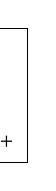
\begin{tikzpicture}[trim axis left, trim axis right]

\begin{axis}[%
width=\figurewidth,
height=\figureheight,
at={(0\figurewidth,0\figureheight)},
scale only axis,
every outer x axis line/.append style={black},
every x tick label/.append style={font=\color{black}},
xmin=9.5,
xmax=16,
xlabel={Time (h)},
every outer y axis line/.append style={black},
every y tick label/.append style={font=\color{black}},
ymin=-0.5,
ymax=0.5,
ylabel={Normalized Book Value},
axis background/.style={fill=white},
axis x line*=bottom,
axis y line*=left,
legend style={legend cell align=left,align=left,draw=black,font=\footnotesize, at={(0.98,0.02)},anchor=south east}
]
\addplot [color=black,solid]
  table[row sep=crcr]{%
9.50027777777778	0\\
9.50583333333333	-0.000231793737116459\\
9.51138888888889	-0.000358042130179537\\
9.51694444444444	-0.000624044133580082\\
9.5225	-0.000704337138179523\\
9.52805555555556	-0.000806368957838699\\
9.53361111111111	-0.000892430694237945\\
9.53916666666667	-0.000668655028491005\\
9.54472222222222	-0.000679814934781309\\
9.55027777777778	-0.000672628843475853\\
9.55583333333333	-0.000745322860736475\\
9.56138888888889	-0.00071655393196346\\
9.56694444444444	-0.000681439299463737\\
9.5725	-0.000695450414574528\\
9.57805555555555	-0.000673883879731663\\
9.58361111111111	-0.000659317409104632\\
9.58916666666667	-0.000621002841693641\\
9.59472222222222	-0.000546146517592216\\
9.60027777777778	-0.000745644539930868\\
9.60583333333333	-0.000766547892410929\\
9.61138888888889	-0.000751569131037688\\
9.61694444444444	-0.000853510681079417\\
9.6225	-0.000831281436831977\\
9.62805555555556	-0.000825117343590587\\
9.63361111111111	-0.000831325026957264\\
9.63916666666667	-0.000804374894810667\\
9.64472222222222	-0.000794067206732141\\
9.65027777777778	-0.000639341901727208\\
9.65583333333333	-0.000606622724905415\\
9.66138888888889	-0.000473285415633407\\
9.66694444444444	-0.000596063833586125\\
9.6725	-0.000464760074997073\\
9.67805555555555	-0.000623819020992622\\
9.68361111111111	-0.000633525944661817\\
9.68916666666667	-0.000444976592099411\\
9.69472222222222	-0.00050328200428873\\
9.70027777777778	-0.000510764229090133\\
9.70583333333333	-0.000720014905398414\\
9.71138888888889	-0.000510787139703539\\
9.71694444444444	-0.000601388040584516\\
9.7225	-0.000510216531229846\\
9.72805555555555	-0.000527103240685611\\
9.73361111111111	-0.000464957574325742\\
9.73916666666667	-0.000414086405420844\\
9.74472222222222	-0.000442162984483963\\
9.75027777777778	-0.000303273727549902\\
9.75583333333333	-0.000319807588345489\\
9.76138888888889	-0.000429585871635108\\
9.76694444444444	-0.000503805162394011\\
9.7725	-0.000438728950765355\\
9.77805555555556	-0.000549918353613399\\
9.78361111111111	-0.000442164634900655\\
9.78916666666667	-0.00054058945893054\\
9.79472222222222	-0.000671441115999816\\
9.80027777777778	-0.000556181514561938\\
9.80583333333333	-0.000553863121377063\\
9.81138888888889	-0.000509252834089091\\
9.81694444444444	-0.000552234080955172\\
9.8225	-0.000548894841679526\\
9.82805555555555	-0.000502966627844881\\
9.83361111111111	-0.00053997615506951\\
9.83916666666667	-0.000563077954824576\\
9.84472222222222	-0.00060496093653184\\
9.85027777777778	-0.000565743244341332\\
9.85583333333333	-0.000441332515205395\\
9.86138888888889	-0.000539759931847072\\
9.86694444444444	-0.000522264980629017\\
9.8725	-0.000508359714266327\\
9.87805555555556	-0.000432992432163659\\
9.88361111111111	-0.000470403210136583\\
9.88916666666667	-0.000440303577289747\\
9.89472222222222	-0.000407402685920766\\
9.90027777777778	-0.000414134063326577\\
9.90583333333333	-0.000397078823199393\\
9.91138888888889	-0.000423827855171921\\
9.91694444444444	-0.000525939230778039\\
9.9225	-0.000511976165591066\\
9.92805555555555	-0.000494488031581475\\
9.93361111111111	-0.000438917341368583\\
9.93916666666667	-0.00038136500767727\\
9.94472222222222	-0.000404726660134691\\
9.95027777777778	-0.000473816892320733\\
9.95583333333333	-0.000452260527121884\\
9.96138888888889	-0.000459018576849046\\
9.96694444444444	-0.000476727516306452\\
9.9725	-0.000478527567585485\\
9.97805555555555	-0.000493796230446208\\
9.98361111111111	-0.000493795472396141\\
9.98916666666667	-0.000563352686366536\\
9.99472222222222	-0.000742969865176413\\
10.0002777777778	-0.000747226491659481\\
10.0058333333333	-0.000682717932618093\\
10.0113888888889	-0.000633298549018391\\
10.0169444444444	-0.000693569143856099\\
10.0225	-0.000636432720171221\\
10.0280555555556	-0.000610508539941157\\
10.0336111111111	-0.000637224163457795\\
10.0391666666667	-0.000816790461895978\\
10.0447222222222	-0.00085027108925062\\
10.0502777777778	-0.000711339738150296\\
10.0558333333333	-0.000715059195751655\\
10.0613888888889	-0.000688495816961177\\
10.0669444444444	-0.000621059112120959\\
10.0725	-0.000637555140431401\\
10.0780555555556	-0.000643652068821887\\
10.0836111111111	-0.000635596714157249\\
10.0891666666667	-0.000589531560579282\\
10.0947222222222	-0.000570172026076454\\
10.1002777777778	-0.000536674809350601\\
10.1058333333333	-0.000582006907978716\\
10.1113888888889	-0.000609715387258736\\
10.1169444444444	-0.0006476608681244\\
10.1225	-0.000636731503331878\\
10.1280555555556	-0.000636755020831825\\
10.1336111111111	-0.000681734295498115\\
10.1391666666667	-0.000697879053012995\\
10.1447222222222	-0.000743194335489084\\
10.1502777777778	-0.000708862488314033\\
10.1558333333333	-0.000755566518815365\\
10.1613888888889	-0.000750778155478637\\
10.1669444444444	-0.000712399374017791\\
10.1725	-0.000704388053086036\\
10.1780555555556	-0.000759592618749361\\
10.1836111111111	-0.00074814059424344\\
10.1891666666667	-0.000762944921240072\\
10.1947222222222	-0.000800253221455827\\
10.2002777777778	-0.000797968884254208\\
10.2058333333333	-0.000838343862346602\\
10.2113888888889	-0.000857952278311092\\
10.2169444444444	-0.000777574673703652\\
10.2225	-0.000796298954289454\\
10.2280555555556	-0.000944208160992943\\
10.2336111111111	-0.000992148137437088\\
10.2391666666667	-0.00101694032544286\\
10.2447222222222	-0.00106373363716361\\
10.2502777777778	-0.00108617682702916\\
10.2558333333333	-0.0010554440018784\\
10.2613888888889	-0.00113364685265971\\
10.2669444444444	-0.00117089929966829\\
10.2725	-0.00123439065111552\\
10.2780555555556	-0.00130108658999972\\
10.2836111111111	-0.00132527443512021\\
10.2891666666667	-0.00131366831755719\\
10.2947222222222	-0.00133170211267486\\
10.3002777777778	-0.00138573070000025\\
10.3058333333333	-0.00149313310410537\\
10.3113888888889	-0.00157028683911364\\
10.3169444444444	-0.00160527957698064\\
10.3225	-0.00160764639324174\\
10.3280555555556	-0.00153539058447671\\
10.3336111111111	-0.00145583774504121\\
10.3391666666667	-0.00147095823672017\\
10.3447222222222	-0.00148318410820325\\
10.3502777777778	-0.00150875880310797\\
10.3558333333333	-0.00153578993183867\\
10.3613888888889	-0.00150993732850968\\
10.3669444444444	-0.00152828643860314\\
10.3725	-0.00152757706891937\\
10.3780555555556	-0.00153490684868596\\
10.3836111111111	-0.00163678758458663\\
10.3891666666667	-0.00171458545238545\\
10.3947222222222	-0.00168106645445942\\
10.4002777777778	-0.00168406225792461\\
10.4058333333333	-0.00163513715915009\\
10.4113888888889	-0.00161125403732254\\
10.4169444444444	-0.00154111718322592\\
10.4225	-0.00154329247963469\\
10.4280555555556	-0.0015665660104669\\
10.4336111111111	-0.00161094524136163\\
10.4391666666667	-0.00166688460384923\\
10.4447222222222	-0.00171716357933516\\
10.4502777777778	-0.00171533201998453\\
10.4558333333333	-0.0017126069164628\\
10.4613888888889	-0.00169750738099772\\
10.4669444444444	-0.00180134039217561\\
10.4725	-0.00179659808634969\\
10.4780555555556	-0.00176947976337227\\
10.4836111111111	-0.00174818512366115\\
10.4891666666667	-0.00172421729367611\\
10.4947222222222	-0.00166623817022238\\
10.5002777777778	-0.0016179276476429\\
10.5058333333333	-0.00164483977840557\\
10.5113888888889	-0.00169228460481041\\
10.5169444444444	-0.00168270671579285\\
10.5225	-0.0017251109882942\\
10.5280555555556	-0.00177011987386777\\
10.5336111111111	-0.00173570920503852\\
10.5391666666667	-0.00172876462084282\\
10.5447222222222	-0.00165735962762759\\
10.5502777777778	-0.00168800209631692\\
10.5558333333333	-0.00173030816757691\\
10.5613888888889	-0.00177893869622936\\
10.5669444444444	-0.00178241765228171\\
10.5725	-0.00176092208989964\\
10.5780555555556	-0.00175880541054851\\
10.5836111111111	-0.00178529382668724\\
10.5891666666667	-0.00175360470523067\\
10.5947222222222	-0.00174975579599601\\
10.6002777777778	-0.00168648050408959\\
10.6058333333333	-0.00167287579947772\\
10.6113888888889	-0.00170936553954903\\
10.6169444444444	-0.00164130172215016\\
10.6225	-0.00162232571126675\\
10.6280555555556	-0.00153011830882621\\
10.6336111111111	-0.00153930355711607\\
10.6391666666667	-0.00151304964870802\\
10.6447222222222	-0.00149347878499939\\
10.6502777777778	-0.00147968555458877\\
10.6558333333333	-0.00145973765876273\\
10.6613888888889	-0.00151885428463827\\
10.6669444444444	-0.00152427600638372\\
10.6725	-0.00145987013887339\\
10.6780555555556	-0.00147278532652673\\
10.6836111111111	-0.0014874089299205\\
10.6891666666667	-0.00143114277035483\\
10.6947222222222	-0.00139891709330464\\
10.7002777777778	-0.00147454734446395\\
10.7058333333333	-0.00147144876777683\\
10.7113888888889	-0.00150990673898954\\
10.7169444444444	-0.00150141254158342\\
10.7225	-0.00148156597143334\\
10.7280555555556	-0.00149982313353025\\
10.7336111111111	-0.00142126398461229\\
10.7391666666667	-0.00136665436657324\\
10.7447222222222	-0.00135205347441714\\
10.7502777777778	-0.00136384386131805\\
10.7558333333333	-0.00130628778851516\\
10.7613888888889	-0.00130188434140011\\
10.7669444444444	-0.00125701662924471\\
10.7725	-0.00123819895788069\\
10.7780555555556	-0.00125213825522563\\
10.7836111111111	-0.00125332190429928\\
10.7891666666667	-0.00122777729959078\\
10.7947222222222	-0.00121946358661718\\
10.8002777777778	-0.00116573600646008\\
10.8058333333333	-0.0011656916382019\\
10.8113888888889	-0.00119731413098778\\
10.8169444444444	-0.0012553643562071\\
10.8225	-0.00123997419350741\\
10.8280555555556	-0.00125045715812155\\
10.8336111111111	-0.00121077540886738\\
10.8391666666667	-0.00124589453076618\\
10.8447222222222	-0.00124192180737026\\
10.8502777777778	-0.00132395274809449\\
10.8558333333333	-0.00129581098396925\\
10.8613888888889	-0.0013176803312599\\
10.8669444444444	-0.00134966722321694\\
10.8725	-0.00137130227346449\\
10.8780555555556	-0.00135385120224429\\
10.8836111111111	-0.00132080722850081\\
10.8891666666667	-0.00130549062930085\\
10.8947222222222	-0.00129746143002119\\
10.9002777777778	-0.00131624601576485\\
10.9058333333333	-0.00132728373171764\\
10.9113888888889	-0.00134397425309618\\
10.9169444444444	-0.00133849823498189\\
10.9225	-0.00134300435255419\\
10.9280555555556	-0.00138634276724103\\
10.9336111111111	-0.00136251249528274\\
10.9391666666667	-0.00133895561592101\\
10.9447222222222	-0.00132999967065184\\
10.9502777777778	-0.00139981718750526\\
10.9558333333333	-0.00139158733985634\\
10.9613888888889	-0.00140211029681903\\
10.9669444444444	-0.00135077332426248\\
10.9725	-0.00135212906169879\\
10.9780555555556	-0.00132221088175222\\
10.9836111111111	-0.0013443121231318\\
10.9891666666667	-0.00142344650309911\\
10.9947222222222	-0.00145904763721949\\
11.0002777777778	-0.00146102629076617\\
11.0058333333333	-0.00140564789975328\\
11.0113888888889	-0.00142708114942114\\
11.0169444444444	-0.00147253614206111\\
11.0225	-0.00147589591716712\\
11.0280555555556	-0.00156097056736493\\
11.0336111111111	-0.00153512196651151\\
11.0391666666667	-0.00151537128365686\\
11.0447222222222	-0.00147996879800782\\
11.0502777777778	-0.00151793109410414\\
11.0558333333333	-0.00152095655735807\\
11.0613888888889	-0.0014840950736752\\
11.0669444444444	-0.00145331752525468\\
11.0725	-0.00143827538507002\\
11.0780555555556	-0.001464242935864\\
11.0836111111111	-0.00145853007785146\\
11.0891666666667	-0.00150118455336368\\
11.0947222222222	-0.00148556024106361\\
11.1002777777778	-0.00152788005296467\\
11.1058333333333	-0.0016096848420013\\
11.1113888888889	-0.00163019175465851\\
11.1169444444444	-0.0015763457146426\\
11.1225	-0.00158003262754369\\
11.1280555555556	-0.00159582682170067\\
11.1336111111111	-0.00160959479232681\\
11.1391666666667	-0.00157620108977141\\
11.1447222222222	-0.00159207558867736\\
11.1502777777778	-0.00167251687301517\\
11.1558333333333	-0.00166966805895208\\
11.1613888888889	-0.00169775585330723\\
11.1669444444444	-0.00172457690905292\\
11.1725	-0.00171182952383719\\
11.1780555555556	-0.00166841946103624\\
11.1836111111111	-0.00170478870117163\\
11.1891666666667	-0.00170052198066761\\
11.1947222222222	-0.00175791914113876\\
11.2002777777778	-0.00172293451179262\\
11.2058333333333	-0.00171379591392473\\
11.2113888888889	-0.00167009819253228\\
11.2169444444444	-0.00172683310845267\\
11.2225	-0.00172478713923552\\
11.2280555555556	-0.0017172127073779\\
11.2336111111111	-0.00170952918422629\\
11.2391666666667	-0.00169528114143236\\
11.2447222222222	-0.00168074672381824\\
11.2502777777778	-0.00172161054908759\\
11.2558333333333	-0.00168996338210969\\
11.2613888888889	-0.0016558303771671\\
11.2669444444444	-0.00166486496694818\\
11.2725	-0.00165889554882681\\
11.2780555555556	-0.00160091728673961\\
11.2836111111111	-0.0015882065551367\\
11.2891666666667	-0.00162778081994741\\
11.2947222222222	-0.00158087651492134\\
11.3002777777778	-0.00157158109877575\\
11.3058333333333	-0.00152789763609884\\
11.3113888888889	-0.00155959845906328\\
11.3169444444444	-0.0015498966591434\\
11.3225	-0.00153061612743932\\
11.3280555555556	-0.0015518567255246\\
11.3336111111111	-0.00158968615464117\\
11.3391666666667	-0.00155374545578046\\
11.3447222222222	-0.00159339536902214\\
11.3502777777778	-0.00157193346946138\\
11.3558333333333	-0.00152361464341089\\
11.3613888888889	-0.00153654195056119\\
11.3669444444444	-0.0015086149639727\\
11.3725	-0.00148346309721048\\
11.3780555555556	-0.00153245904826182\\
11.3836111111111	-0.00147203447125444\\
11.3891666666667	-0.00144841053559475\\
11.3947222222222	-0.00140524047373203\\
11.4002777777778	-0.0014147056547329\\
11.4058333333333	-0.0013987981024759\\
11.4113888888889	-0.00140885399109147\\
11.4169444444444	-0.00140286311282689\\
11.4225	-0.00138573419596999\\
11.4280555555556	-0.00137202799785796\\
11.4336111111111	-0.00136377867263482\\
11.4391666666667	-0.00138586746047953\\
11.4447222222222	-0.00138738801869098\\
11.4502777777778	-0.00139297080029588\\
11.4558333333333	-0.00141258164126745\\
11.4613888888889	-0.00143175055493339\\
11.4669444444444	-0.0014412317092215\\
11.4725	-0.0013879455307807\\
11.4780555555556	-0.00139470479389736\\
11.4836111111111	-0.00141029640125312\\
11.4891666666667	-0.00139514136936281\\
11.4947222222222	-0.00138959770670333\\
11.5002777777778	-0.00139786311584056\\
11.5058333333333	-0.00141203764003917\\
11.5113888888889	-0.00135699676132417\\
11.5169444444444	-0.00125732337961482\\
11.5225	-0.00137775005669516\\
11.5280555555556	-0.00132910780739359\\
11.5336111111111	-0.0012955372717226\\
11.5391666666667	-0.00136161478466368\\
11.5447222222222	-0.00136530652357159\\
11.5502777777778	-0.00133654123632365\\
11.5558333333333	-0.0013022664619704\\
11.5613888888889	-0.00128598626701937\\
11.5669444444444	-0.00122532941858589\\
11.5725	-0.00124378216512211\\
11.5780555555556	-0.00128494090356357\\
11.5836111111111	-0.0013415528438937\\
11.5891666666667	-0.00136339895779403\\
11.5947222222222	-0.00133257239636186\\
11.6002777777778	-0.00139389746490703\\
11.6058333333333	-0.00140335376899403\\
11.6113888888889	-0.00138422221427537\\
11.6169444444444	-0.00143436948945175\\
11.6225	-0.00145971340086215\\
11.6280555555556	-0.00146940066108969\\
11.6336111111111	-0.00148668610441349\\
11.6391666666667	-0.00150143006750003\\
11.6447222222222	-0.00147477830756626\\
11.6502777777778	-0.00140777662591363\\
11.6558333333333	-0.00145394005025723\\
11.6613888888889	-0.00148109521439455\\
11.6669444444444	-0.00146695940805786\\
11.6725	-0.00146992703925153\\
11.6780555555556	-0.00151868926070553\\
11.6836111111111	-0.00152435680190777\\
11.6891666666667	-0.00154555811000945\\
11.6947222222222	-0.00156323114253742\\
11.7002777777778	-0.00153258189660144\\
11.7058333333333	-0.00150489329482728\\
11.7113888888889	-0.00148281087327629\\
11.7169444444444	-0.00152851558983869\\
11.7225	-0.00148980738461979\\
11.7280555555556	-0.0015527731802164\\
11.7336111111111	-0.00153816708386423\\
11.7391666666667	-0.00151339053875488\\
11.7447222222222	-0.00154211169025553\\
11.7502777777778	-0.001569052231015\\
11.7558333333333	-0.00149964017168724\\
11.7613888888889	-0.00153333978524206\\
11.7669444444444	-0.00151558481591207\\
11.7725	-0.00152696928229223\\
11.7780555555556	-0.00150967738659213\\
11.7836111111111	-0.00141585204167483\\
11.7891666666667	-0.00145243745023871\\
11.7947222222222	-0.00144825963536299\\
11.8002777777778	-0.00150162476424553\\
11.8058333333333	-0.00146011959257186\\
11.8113888888889	-0.00144953935213177\\
11.8169444444444	-0.00149637405191372\\
11.8225	-0.00148000585615793\\
11.8280555555556	-0.00146524042907747\\
11.8336111111111	-0.00143050325342697\\
11.8391666666667	-0.00147241768845663\\
11.8447222222222	-0.00145291891378141\\
11.8502777777778	-0.00142846704448529\\
11.8558333333333	-0.00144789769935516\\
11.8613888888889	-0.0014336696603986\\
11.8669444444444	-0.0014063080428236\\
11.8725	-0.00138643204979794\\
11.8780555555556	-0.00135635411074408\\
11.8836111111111	-0.00131093436785978\\
11.8891666666667	-0.00123124921848694\\
11.8947222222222	-0.00124924176198793\\
11.9002777777778	-0.0012765811712443\\
11.9058333333333	-0.00138265424509798\\
11.9113888888889	-0.00138017512436495\\
11.9169444444444	-0.00136816456036037\\
11.9225	-0.0013543315344835\\
11.9280555555556	-0.00133117665615579\\
11.9336111111111	-0.0013015482437958\\
11.9391666666667	-0.00127504355087305\\
11.9447222222222	-0.00122777026421528\\
11.9502777777778	-0.00125982037694017\\
11.9558333333333	-0.00121032819370592\\
11.9613888888889	-0.00126365128416872\\
11.9669444444444	-0.00128160789218923\\
11.9725	-0.00126796943854646\\
11.9780555555556	-0.00121741424373034\\
11.9836111111111	-0.0012139977937442\\
11.9891666666667	-0.00122431010383262\\
11.9947222222222	-0.00127409433169468\\
12.0002777777778	-0.0011875966684527\\
12.0058333333333	-0.00122813029238344\\
12.0113888888889	-0.00119210120527435\\
12.0169444444444	-0.00125596076887113\\
12.0225	-0.00124760592788831\\
12.0280555555556	-0.00126762142573167\\
12.0336111111111	-0.00130121077186152\\
12.0391666666667	-0.00127328753515665\\
12.0447222222222	-0.00130800698716971\\
12.0502777777778	-0.00127681622700804\\
12.0558333333333	-0.00133714458961232\\
12.0613888888889	-0.00136671157840085\\
12.0669444444444	-0.00139374382956525\\
12.0725	-0.00135429012106969\\
12.0780555555556	-0.00133572423542605\\
12.0836111111111	-0.00133953001303033\\
12.0891666666667	-0.00143324542577505\\
12.0947222222222	-0.00144824190743109\\
12.1002777777778	-0.0013972233396301\\
12.1058333333333	-0.00139143182192425\\
12.1113888888889	-0.00139947421762499\\
12.1169444444444	-0.00145315787022804\\
12.1225	-0.00145051068621405\\
12.1280555555556	-0.00148649506126641\\
12.1336111111111	-0.00146776368553969\\
12.1391666666667	-0.00146774824542883\\
12.1447222222222	-0.00149308464426146\\
12.1502777777778	-0.00150721836792067\\
12.1558333333333	-0.00152736308660784\\
12.1613888888889	-0.00149633567593044\\
12.1669444444444	-0.00150273129981293\\
12.1725	-0.00150004120100145\\
12.1780555555556	-0.0015295785575653\\
12.1836111111111	-0.00153310853449751\\
12.1891666666667	-0.00152966814543731\\
12.1947222222222	-0.00149855231290252\\
12.2002777777778	-0.00147823616751896\\
12.2058333333333	-0.00147896649616375\\
12.2113888888889	-0.00147111286492374\\
12.2169444444444	-0.00151516505969529\\
12.2225	-0.00154913100591603\\
12.2280555555556	-0.00152252919921925\\
12.2336111111111	-0.00150228946163278\\
12.2391666666667	-0.00148708829335775\\
12.2447222222222	-0.00142653412658278\\
12.2502777777778	-0.00143813928103864\\
12.2558333333333	-0.00145467710776381\\
12.2613888888889	-0.00146016057534071\\
12.2669444444444	-0.00148525257484133\\
12.2725	-0.00147414089396247\\
12.2780555555556	-0.00145265200606892\\
12.2836111111111	-0.00145913460078462\\
12.2891666666667	-0.00141066735161643\\
12.2947222222222	-0.00138946498071812\\
12.3002777777778	-0.00137166710036019\\
12.3058333333333	-0.00133375678128145\\
12.3113888888889	-0.00131390035469336\\
12.3169444444444	-0.00128484877334556\\
12.3225	-0.00129639560806727\\
12.3280555555556	-0.00128215070212767\\
12.3336111111111	-0.0012965255703058\\
12.3391666666667	-0.001305923249316\\
12.3447222222222	-0.00128146087737369\\
12.3502777777778	-0.0013190214212625\\
12.3558333333333	-0.00134464921541488\\
12.3613888888889	-0.00135135706645828\\
12.3669444444444	-0.00139245321994541\\
12.3725	-0.00132425685024573\\
12.3780555555556	-0.00133704769303444\\
12.3836111111111	-0.00131681633040603\\
12.3891666666667	-0.0013245481229015\\
12.3947222222222	-0.00137704990232557\\
12.4002777777778	-0.00135284215034748\\
12.4058333333333	-0.00132501079205516\\
12.4113888888889	-0.00132427742297359\\
12.4169444444444	-0.00134199655744904\\
12.4225	-0.00134740210310358\\
12.4280555555556	-0.00137679561692572\\
12.4336111111111	-0.00137175724199323\\
12.4391666666667	-0.00137399366344249\\
12.4447222222222	-0.00135851708587487\\
12.4502777777778	-0.0013795251869535\\
12.4558333333333	-0.0014115354112445\\
12.4613888888889	-0.00138728809884681\\
12.4669444444444	-0.00140589561404392\\
12.4725	-0.00142976271636497\\
12.4780555555556	-0.00142027559905622\\
12.4836111111111	-0.00143722188646911\\
12.4891666666667	-0.00134466873437811\\
12.4947222222222	-0.00129548568557869\\
12.5002777777778	-0.00136606218581437\\
12.5058333333333	-0.00134687108000686\\
12.5113888888889	-0.00136807074516432\\
12.5169444444444	-0.00132051171781256\\
12.5225	-0.0012936404618733\\
12.5280555555556	-0.00132701328288376\\
12.5336111111111	-0.00132705262505084\\
12.5391666666667	-0.00132515147226364\\
12.5447222222222	-0.00124941585647209\\
12.5502777777778	-0.0012008677712092\\
12.5558333333333	-0.00123365455324309\\
12.5613888888889	-0.00124733408714162\\
12.5669444444444	-0.00118764790668613\\
12.5725	-0.00112791569780202\\
12.5780555555556	-0.00103883888558387\\
12.5836111111111	-0.00108154332840127\\
12.5891666666667	-0.00102833163123262\\
12.5947222222222	-0.00099301041231481\\
12.6002777777778	-0.00102111655096415\\
12.6058333333333	-0.00103494553351735\\
12.6113888888889	-0.00102925098671114\\
12.6169444444444	-0.00103065143404668\\
12.6225	-0.00103248239507592\\
12.6280555555556	-0.00102372228782865\\
12.6336111111111	-0.00102107584459465\\
12.6391666666667	-0.000999714354949721\\
12.6447222222222	-0.000929042751573572\\
12.6502777777778	-0.00097084824842042\\
12.6558333333333	-0.000945594798557714\\
12.6613888888889	-0.000938783536369892\\
12.6669444444444	-0.000992058703715548\\
12.6725	-0.000886436054219231\\
12.6780555555556	-0.000849732825725424\\
12.6836111111111	-0.000896130318963517\\
12.6891666666667	-0.000917043996663036\\
12.6947222222222	-0.000897544690625196\\
12.7002777777778	-0.000896390415166315\\
12.7058333333333	-0.000857871285157241\\
12.7113888888889	-0.000872691540217296\\
12.7169444444444	-0.000893149805895832\\
12.7225	-0.000865030947968526\\
12.7280555555556	-0.000857690500245867\\
12.7336111111111	-0.00085338126293566\\
12.7391666666667	-0.000857501804570671\\
12.7447222222222	-0.000875099164382998\\
12.7502777777778	-0.000866629576940503\\
12.7558333333333	-0.000923360211912083\\
12.7613888888889	-0.000886256109344341\\
12.7669444444444	-0.000949011013113399\\
12.7725	-0.000984408112574497\\
12.7780555555556	-0.000995835467355377\\
12.7836111111111	-0.000978041448412625\\
12.7891666666667	-0.000923273272620984\\
12.7947222222222	-0.000861153296078609\\
12.8002777777778	-0.000811744814160575\\
12.8058333333333	-0.000771135517302568\\
12.8113888888889	-0.000766352272603577\\
12.8169444444444	-0.000817821617015158\\
12.8225	-0.000831179383467995\\
12.8280555555556	-0.000817754435956664\\
12.8336111111111	-0.000771481861372436\\
12.8391666666667	-0.000806677446545945\\
12.8447222222222	-0.000775752569288746\\
12.8502777777778	-0.000800653848344823\\
12.8558333333333	-0.000769040493637574\\
12.8613888888889	-0.000778406572635282\\
12.8669444444444	-0.000787528175687946\\
12.8725	-0.000771268597614339\\
12.8780555555556	-0.00075843659862318\\
12.8836111111111	-0.000781804529078278\\
12.8891666666667	-0.000805916116337957\\
12.8947222222222	-0.000783954047150814\\
12.9002777777778	-0.000724088526057098\\
12.9058333333333	-0.000726943397987512\\
12.9113888888889	-0.00081927066064702\\
12.9169444444444	-0.000855222880272843\\
12.9225	-0.000816141241411716\\
12.9280555555556	-0.000795430889430015\\
12.9336111111111	-0.000784307308303922\\
12.9391666666667	-0.000797966071879763\\
12.9447222222222	-0.000811328094770358\\
12.9502777777778	-0.000801583959468943\\
12.9558333333333	-0.000768227298502788\\
12.9613888888889	-0.000739439646497808\\
12.9669444444444	-0.000733991899960706\\
12.9725	-0.000692136737565741\\
12.9780555555556	-0.000722755095661665\\
12.9836111111111	-0.000724188116026592\\
12.9891666666667	-0.000734409645590794\\
12.9947222222222	-0.000665890916136114\\
13.0002777777778	-0.000880762856904305\\
13.0058333333333	-0.000893088796747099\\
13.0113888888889	-0.000891256507604132\\
13.0169444444444	-0.000905986170811612\\
13.0225	-0.000902904131966697\\
13.0280555555556	-0.000939876956422614\\
13.0336111111111	-0.000907434400238549\\
13.0391666666667	-0.000925373169094246\\
13.0447222222222	-0.0008973200102802\\
13.0502777777778	-0.000881514560182928\\
13.0558333333333	-0.000841155386032022\\
13.0613888888889	-0.000818141317658116\\
13.0669444444444	-0.000813193552280045\\
13.0725	-0.000755883034038396\\
13.0780555555556	-0.000739125149015307\\
13.0836111111111	-0.000759155594518446\\
13.0891666666667	-0.000734179608488761\\
13.0947222222222	-0.000727824525892262\\
13.1002777777778	-0.000716974159221451\\
13.1058333333333	-0.000731901185583639\\
13.1113888888889	-0.000725622567307793\\
13.1169444444444	-0.000722736170948757\\
13.1225	-0.000697985501624254\\
13.1280555555556	-0.000723445067169703\\
13.1336111111111	-0.000755895492339009\\
13.1391666666667	-0.000733592144611772\\
13.1447222222222	-0.000733994225628143\\
13.1502777777778	-0.000699292646816674\\
13.1558333333333	-0.000751995881791756\\
13.1613888888889	-0.000761311609878579\\
13.1669444444444	-0.000795224078252832\\
13.1725	-0.000807242721475698\\
13.1780555555556	-0.000782783860407532\\
13.1836111111111	-0.000825311927996064\\
13.1891666666667	-0.000797403832400456\\
13.1947222222222	-0.000819928100638023\\
13.2002777777778	-0.000825779601351995\\
13.2058333333333	-0.00084072501522825\\
13.2113888888889	-0.000855781713938963\\
13.2169444444444	-0.000814888914132839\\
13.2225	-0.000782596179180084\\
13.2280555555556	-0.000784391486834513\\
13.2336111111111	-0.000756654701047355\\
13.2391666666667	-0.000765367516353144\\
13.2447222222222	-0.00076756735650263\\
13.2502777777778	-0.000790956703994428\\
13.2558333333333	-0.000791345477523464\\
13.2613888888889	-0.00073163968125356\\
13.2669444444444	-0.000750857891910206\\
13.2725	-0.000733146689698039\\
13.2780555555556	-0.000731483875883066\\
13.2836111111111	-0.000768494180141799\\
13.2891666666667	-0.000801226852823911\\
13.2947222222222	-0.000816765476016945\\
13.3002777777778	-0.000821894220456976\\
13.3058333333333	-0.000870089680503061\\
13.3113888888889	-0.000870592418213523\\
13.3169444444444	-0.000800141361771756\\
13.3225	-0.000804678703719253\\
13.3280555555556	-0.000806685173652788\\
13.3336111111111	-0.000763222459736035\\
13.3391666666667	-0.000760951098592089\\
13.3447222222222	-0.000740920273672008\\
13.3502777777778	-0.000730076326146967\\
13.3558333333333	-0.000750241085710424\\
13.3613888888889	-0.000773830767523354\\
13.3669444444444	-0.00075983990142281\\
13.3725	-0.000750667586721043\\
13.3780555555556	-0.000708439777870606\\
13.3836111111111	-0.000727336784481669\\
13.3891666666667	-0.000706017164548767\\
13.3947222222222	-0.00070972624164789\\
13.4002777777778	-0.000712127357542891\\
13.4058333333333	-0.000763324657780839\\
13.4113888888889	-0.000743098180216784\\
13.4169444444444	-0.000775370494847993\\
13.4225	-0.000801604471813877\\
13.4280555555556	-0.000817447075930899\\
13.4336111111111	-0.0007649550226283\\
13.4391666666667	-0.000744183242297525\\
13.4447222222222	-0.000744365131631008\\
13.4502777777778	-0.000713003886175234\\
13.4558333333333	-0.000754872713205068\\
13.4613888888889	-0.000757053778554062\\
13.4669444444444	-0.00076950468631265\\
13.4725	-0.000783926130787371\\
13.4780555555556	-0.000775929870759251\\
13.4836111111111	-0.000790631442473266\\
13.4891666666667	-0.000803276084516469\\
13.4947222222222	-0.000823607851956121\\
13.5002777777778	-0.000799415562513839\\
13.5058333333333	-0.000794362167035101\\
13.5113888888889	-0.000769725815779165\\
13.5169444444444	-0.000791916335633136\\
13.5225	-0.000827910202000459\\
13.5280555555556	-0.000824521078098495\\
13.5336111111111	-0.000880706604443726\\
13.5391666666667	-0.000844207847943812\\
13.5447222222222	-0.000857821758354249\\
13.5502777777778	-0.000808736892763173\\
13.5558333333333	-0.000817641584635487\\
13.5613888888889	-0.000796394337649664\\
13.5669444444444	-0.000820298795491281\\
13.5725	-0.000828050962069837\\
13.5780555555556	-0.000838861566224147\\
13.5836111111111	-0.000835930481312697\\
13.5891666666667	-0.000825008134958893\\
13.5947222222222	-0.000874321179951676\\
13.6002777777778	-0.000865673810236167\\
13.6058333333333	-0.000908138262671554\\
13.6113888888889	-0.000922955746936793\\
13.6169444444444	-0.000923078021851431\\
13.6225	-0.000898547871010402\\
13.6280555555556	-0.000897604956752951\\
13.6336111111111	-0.000888058413861192\\
13.6391666666667	-0.000922673239127092\\
13.6447222222222	-0.000978636348743289\\
13.6502777777778	-0.000963419610954919\\
13.6558333333333	-0.000954579407484779\\
13.6613888888889	-0.000979314667873932\\
13.6669444444444	-0.000969506520876462\\
13.6725	-0.000952204174828664\\
13.6780555555556	-0.000957251332325937\\
13.6836111111111	-0.000950479169728236\\
13.6891666666667	-0.000930169044787599\\
13.6947222222222	-0.000892229941459433\\
13.7002777777778	-0.000915081781118321\\
13.7058333333333	-0.000930302358073121\\
13.7113888888889	-0.000977699874417093\\
13.7169444444444	-0.000906625848298814\\
13.7225	-0.000926654773821811\\
13.7280555555556	-0.000945448812812888\\
13.7336111111111	-0.0009009862157906\\
13.7391666666667	-0.000905027808887016\\
13.7447222222222	-0.000890288819310858\\
13.7502777777778	-0.000869969545258531\\
13.7558333333333	-0.000918298515835581\\
13.7613888888889	-0.000929661215698152\\
13.7669444444444	-0.000915899230795714\\
13.7725	-0.000934915425896854\\
13.7780555555556	-0.000968322070935557\\
13.7836111111111	-0.00101785122097509\\
13.7891666666667	-0.000989662305204475\\
13.7947222222222	-0.000961344950377696\\
13.8002777777778	-0.000973076153111263\\
13.8058333333333	-0.000932887253212722\\
13.8113888888889	-0.00090327121554401\\
13.8169444444444	-0.000911285379803339\\
13.8225	-0.000910018888000241\\
13.8280555555556	-0.000873412193167167\\
13.8336111111111	-0.000888484275511359\\
13.8391666666667	-0.000879712554306633\\
13.8447222222222	-0.000882621743782508\\
13.8502777777778	-0.000871205086741877\\
13.8558333333333	-0.000847712637590536\\
13.8613888888889	-0.000819191274978093\\
13.8669444444444	-0.000801546669570108\\
13.8725	-0.000824969067725112\\
13.8780555555556	-0.000846725357931399\\
13.8836111111111	-0.00086859706929765\\
13.8891666666667	-0.000855452419997405\\
13.8947222222222	-0.000813236053372357\\
13.9002777777778	-0.000814641942060268\\
13.9058333333333	-0.000832794807409054\\
13.9113888888889	-0.000833610232570892\\
13.9169444444444	-0.000843216181419582\\
13.9225	-0.000852058548136747\\
13.9280555555556	-0.00085934339435445\\
13.9336111111111	-0.000919072532188259\\
13.9391666666667	-0.000929975971765473\\
13.9447222222222	-0.000931599965238061\\
13.9502777777778	-0.00090887206156498\\
13.9558333333333	-0.000885526969452433\\
13.9613888888889	-0.000876752116574564\\
13.9669444444444	-0.000922007673284098\\
13.9725	-0.000902714389181658\\
13.9780555555556	-0.000923752814116274\\
13.9836111111111	-0.000939559038798499\\
13.9891666666667	-0.000950138510526277\\
13.9947222222222	-0.000972705294648324\\
14.0002777777778	-0.000974627201243861\\
14.0058333333333	-0.000931524335986533\\
14.0113888888889	-0.000956917931165591\\
14.0169444444444	-0.000942024167264965\\
14.0225	-0.000991808331958666\\
14.0280555555556	-0.000939534006209386\\
14.0336111111111	-0.000937270073895546\\
14.0391666666667	-0.000943493007879881\\
14.0447222222222	-0.000976272099003195\\
14.0502777777778	-0.000945139405585604\\
14.0558333333333	-0.000959177233612607\\
14.0613888888889	-0.0009390104469299\\
14.0669444444444	-0.000904863817525747\\
14.0725	-0.000931469565164544\\
14.0780555555556	-0.000959799551380147\\
14.0836111111111	-0.000981404480130843\\
14.0891666666667	-0.00095172824487233\\
14.0947222222222	-0.000939192004852929\\
14.1002777777778	-0.000941515074782573\\
14.1058333333333	-0.000959344375947913\\
14.1113888888889	-0.000971714049402439\\
14.1169444444444	-0.000931767282381757\\
14.1225	-0.000944516744454504\\
14.1280555555556	-0.000942889794863677\\
14.1336111111111	-0.000938933072078485\\
14.1391666666667	-0.000947653266787252\\
14.1447222222222	-0.000917198272750941\\
14.1502777777778	-0.000929793945662949\\
14.1558333333333	-0.000953331979810401\\
14.1613888888889	-0.000907308443310439\\
14.1669444444444	-0.000910725392762934\\
14.1725	-0.00091067218813945\\
14.1780555555556	-0.00089133569302835\\
14.1836111111111	-0.000913380195219249\\
14.1891666666667	-0.000919217187533516\\
14.1947222222222	-0.000961312724179431\\
14.2002777777778	-0.000939615451941878\\
14.2058333333333	-0.000850791048497723\\
14.2113888888889	-0.000865370251288855\\
14.2169444444444	-0.000906379787698142\\
14.2225	-0.000931889852143208\\
14.2280555555556	-0.000981500368408161\\
14.2336111111111	-0.000984950959260988\\
14.2391666666667	-0.000974408186733888\\
14.2447222222222	-0.000942976683554253\\
14.2502777777778	-0.000929275367101412\\
14.2558333333333	-0.000849645349276007\\
14.2613888888889	-0.000890716894624832\\
14.2669444444444	-0.000831205439617455\\
14.2725	-0.000835183351104662\\
14.2780555555556	-0.00084815250593484\\
14.2836111111111	-0.000854083731809618\\
14.2891666666667	-0.000781512025652686\\
14.2947222222222	-0.000746125069731707\\
14.3002777777778	-0.000751769294634053\\
14.3058333333333	-0.000755086587570952\\
14.3113888888889	-0.000779311766464508\\
14.3169444444444	-0.000786007455024884\\
14.3225	-0.000794905047811323\\
14.3280555555556	-0.000823448759777134\\
14.3336111111111	-0.000802829696765039\\
14.3391666666667	-0.00085399358266236\\
14.3447222222222	-0.000850442219265557\\
14.3502777777778	-0.000797817423815905\\
14.3558333333333	-0.000789777100734357\\
14.3613888888889	-0.000796081751362254\\
14.3669444444444	-0.000804277074385462\\
14.3725	-0.000832781050224551\\
14.3780555555556	-0.000845975170955415\\
14.3836111111111	-0.000931641777582759\\
14.3891666666667	-0.000896696335034974\\
14.3947222222222	-0.000864384795618789\\
14.4002777777778	-0.000867458810520638\\
14.4058333333333	-0.000846677534686147\\
14.4113888888889	-0.000864392854659335\\
14.4169444444444	-0.000834525327540581\\
14.4225	-0.000802263160829764\\
14.4280555555556	-0.000771925621412262\\
14.4336111111111	-0.000732082366783793\\
14.4391666666667	-0.000761614959560508\\
14.4447222222222	-0.000743067061297231\\
14.4502777777778	-0.000745211110570132\\
14.4558333333333	-0.000811420498405879\\
14.4613888888889	-0.000787490169098737\\
14.4669444444444	-0.000776438446260519\\
14.4725	-0.000774329033453869\\
14.4780555555556	-0.000729813804422386\\
14.4836111111111	-0.00071788169331144\\
14.4891666666667	-0.000688805115670488\\
14.4947222222222	-0.00067018626710158\\
14.5002777777778	-0.000713376420518275\\
14.5058333333333	-0.000720467121745116\\
14.5113888888889	-0.00071044481002569\\
14.5169444444444	-0.000703860787250155\\
14.5225	-0.000679056003980216\\
14.5280555555556	-0.000661040067853835\\
14.5336111111111	-0.000662060441608658\\
14.5391666666667	-0.000641503229247831\\
14.5447222222222	-0.000687257574209732\\
14.5502777777778	-0.000677610941994922\\
14.5558333333333	-0.000668556029144507\\
14.5613888888889	-0.000688893930262058\\
14.5669444444444	-0.000699558463449601\\
14.5725	-0.000689233536389944\\
14.5780555555556	-0.000732476815847205\\
14.5836111111111	-0.000734451606569708\\
14.5891666666667	-0.000715481566144316\\
14.5947222222222	-0.000682553768361127\\
14.6002777777778	-0.000721432521062382\\
14.6058333333333	-0.000733547294996195\\
14.6113888888889	-0.000759961262085218\\
14.6169444444444	-0.000747256343085145\\
14.6225	-0.000718483753800681\\
14.6280555555556	-0.000699252908269332\\
14.6336111111111	-0.000658390854887947\\
14.6391666666667	-0.000694585048392926\\
14.6447222222222	-0.000697457648269117\\
14.6502777777778	-0.000726575219371695\\
14.6558333333333	-0.000772519799196347\\
14.6613888888889	-0.000766612192956928\\
14.6669444444444	-0.00073490524864317\\
14.6725	-0.000770250038339415\\
14.6780555555556	-0.000782616013764725\\
14.6836111111111	-0.000789569478604979\\
14.6891666666667	-0.000749868932496844\\
14.6947222222222	-0.000773514638411354\\
14.7002777777778	-0.000773049693161054\\
14.7058333333333	-0.000787710033599787\\
14.7113888888889	-0.000762787591044534\\
14.7169444444444	-0.00081391818954879\\
14.7225	-0.00077363372094541\\
14.7280555555556	-0.000757502683962352\\
14.7336111111111	-0.000763290526041072\\
14.7391666666667	-0.000746423519751516\\
14.7447222222222	-0.000770246177498657\\
14.7502777777778	-0.000784357734631591\\
14.7558333333333	-0.000776112193211387\\
14.7613888888889	-0.000776360781644225\\
14.7669444444444	-0.00079342107451208\\
14.7725	-0.00078644434846642\\
14.7780555555556	-0.000771334039090243\\
14.7836111111111	-0.000728570635386894\\
14.7891666666667	-0.000716255216802075\\
14.7947222222222	-0.000690898292048603\\
14.8002777777778	-0.000689687101666281\\
14.8058333333333	-0.000705497115836784\\
14.8113888888889	-0.000713917618840543\\
14.8169444444444	-0.000720694216044149\\
14.8225	-0.000724508452544126\\
14.8280555555556	-0.000693259015288938\\
14.8336111111111	-0.000666548039820469\\
14.8391666666667	-0.000662296878381374\\
14.8447222222222	-0.000695917535371349\\
14.8502777777778	-0.000724561183781836\\
14.8558333333333	-0.000670370393457631\\
14.8613888888889	-0.00069463761522337\\
14.8669444444444	-0.000653998504053233\\
14.8725	-0.000712841298411537\\
14.8780555555556	-0.000720371827439892\\
14.8836111111111	-0.000710292565541448\\
14.8891666666667	-0.000698907737670118\\
14.8947222222222	-0.000650564709281154\\
14.9002777777778	-0.000656097330571148\\
14.9058333333333	-0.000695845845207654\\
14.9113888888889	-0.000720992050821434\\
14.9169444444444	-0.000682229438922266\\
14.9225	-0.000690158725149548\\
14.9280555555556	-0.000658537577055807\\
14.9336111111111	-0.000656205061669413\\
14.9391666666667	-0.000615736618507112\\
14.9447222222222	-0.000644163562371292\\
14.9502777777778	-0.00068071594361252\\
14.9558333333333	-0.000689035372611557\\
14.9613888888889	-0.000727125947845408\\
14.9669444444444	-0.000673616313852876\\
14.9725	-0.000684872263432057\\
14.9780555555556	-0.000728187013410708\\
14.9836111111111	-0.000690682942807275\\
14.9891666666667	-0.000662104018542831\\
14.9947222222222	-0.000660102126715523\\
15.0002777777778	-0.000722169163480002\\
15.0058333333333	-0.00074155243393903\\
15.0113888888889	-0.000773265258719236\\
15.0169444444444	-0.000780315673560628\\
15.0225	-0.000792171234575201\\
15.0280555555556	-0.000740077802549699\\
15.0336111111111	-0.000741144952790873\\
15.0391666666667	-0.000790831439186457\\
15.0447222222222	-0.000797266903051153\\
15.0502777777778	-0.000774041277731952\\
15.0558333333333	-0.000771645635563423\\
15.0613888888889	-0.000759254812162991\\
15.0669444444444	-0.000768050318506464\\
15.0725	-0.00076198567326069\\
15.0780555555556	-0.00078477455013326\\
15.0836111111111	-0.000785726999666503\\
15.0891666666667	-0.000737432657445081\\
15.0947222222222	-0.000684043774249132\\
15.1002777777778	-0.000671838373585087\\
15.1058333333333	-0.000745988942030262\\
15.1113888888889	-0.000717194001435995\\
15.1169444444444	-0.00080411711674\\
15.1225	-0.000765878886125448\\
15.1280555555556	-0.000759553169743743\\
15.1336111111111	-0.000826818185269307\\
15.1391666666667	-0.000849812082176493\\
15.1447222222222	-0.000814716663595338\\
15.1502777777778	-0.000836347112174174\\
15.1558333333333	-0.000818738154254373\\
15.1613888888889	-0.000855651010461367\\
15.1669444444444	-0.000843717365753838\\
15.1725	-0.000814874859461745\\
15.1780555555556	-0.000798451556125013\\
15.1836111111111	-0.000785267019975833\\
15.1891666666667	-0.000765040556158891\\
15.1947222222222	-0.000782374837231203\\
15.2002777777778	-0.000809072213043938\\
15.2058333333333	-0.000831312758320601\\
15.2113888888889	-0.00084791443048049\\
15.2169444444444	-0.000787878941839182\\
15.2225	-0.000807149764354365\\
15.2280555555556	-0.000760352184181357\\
15.2336111111111	-0.000790329216791674\\
15.2391666666667	-0.000767178580900918\\
15.2447222222222	-0.000765007723960709\\
15.2502777777778	-0.000762278034621366\\
15.2558333333333	-0.000743718321368547\\
15.2613888888889	-0.000743875528590121\\
15.2669444444444	-0.00072001646485631\\
15.2725	-0.000704984087067206\\
15.2780555555556	-0.000656841052787738\\
15.2836111111111	-0.000628388130713864\\
15.2891666666667	-0.000628776576111156\\
15.2947222222222	-0.000637280158134579\\
15.3002777777778	-0.000668986957623519\\
15.3058333333333	-0.000674299114593491\\
15.3113888888889	-0.000671082528110323\\
15.3169444444444	-0.000621536434402437\\
15.3225	-0.000659585367933091\\
15.3280555555556	-0.00068991420921416\\
15.3336111111111	-0.000735004485263646\\
15.3391666666667	-0.000649487309650532\\
15.3447222222222	-0.000677684581672389\\
15.3502777777778	-0.000708153257196642\\
15.3558333333333	-0.000761535022737236\\
15.3613888888889	-0.000748809288431795\\
15.3669444444444	-0.000756551955936269\\
15.3725	-0.000787695511884623\\
15.3780555555556	-0.000726903149178781\\
15.3836111111111	-0.000714560466251846\\
15.3891666666667	-0.000740602140316349\\
15.3947222222222	-0.000756802475986085\\
15.4002777777778	-0.000769678248804251\\
15.4058333333333	-0.00084526014304831\\
15.4113888888889	-0.000843129771125772\\
15.4169444444444	-0.000834713514815455\\
15.4225	-0.000807091159332085\\
15.4280555555556	-0.000814651775443154\\
15.4336111111111	-0.000830923278634099\\
15.4391666666667	-0.000799399603512274\\
15.4447222222222	-0.000834631243565309\\
15.4502777777778	-0.000767594347568346\\
15.4558333333333	-0.000738915503602722\\
15.4613888888889	-0.000748271849760562\\
15.4669444444444	-0.000719177710275187\\
15.4725	-0.000773657902081726\\
15.4780555555556	-0.000797923581546733\\
15.4836111111111	-0.000790802956902259\\
15.4891666666667	-0.000761112991887414\\
15.4947222222222	-0.000766721063812703\\
15.5002777777778	-0.000776828964460852\\
15.5058333333333	-0.000782402048472242\\
15.5113888888889	-0.000847565438908626\\
15.5169444444444	-0.000832520339935972\\
15.5225	-0.000819613735494884\\
15.5280555555556	-0.000846060110821889\\
15.5336111111111	-0.000827755440233613\\
15.5391666666667	-0.000815439557693476\\
15.5447222222222	-0.000838785074170567\\
15.5502777777778	-0.000795221418902314\\
15.5558333333333	-0.000784401060595297\\
15.5613888888889	-0.000856952479363904\\
15.5669444444444	-0.000867560990537641\\
15.5725	-0.00088596729598367\\
15.5780555555556	-0.00084763377448549\\
15.5836111111111	-0.000855937148092067\\
15.5891666666667	-0.00087428093856623\\
15.5947222222222	-0.000908308658416623\\
15.6002777777778	-0.000894366659356605\\
15.6058333333333	-0.000957350948875169\\
15.6113888888889	-0.000905181426948398\\
15.6169444444444	-0.000913889204942619\\
15.6225	-0.000956003479475886\\
15.6280555555556	-0.000948908213492694\\
15.6336111111111	-0.000947358951854937\\
15.6391666666667	-0.000895027946952287\\
15.6447222222222	-0.000904683205847689\\
15.6502777777778	-0.000908236098068893\\
15.6558333333333	-0.000849439070425673\\
15.6613888888889	-0.000879648706759939\\
15.6669444444444	-0.000932796913614142\\
15.6725	-0.00093359526445147\\
15.6780555555556	-0.000887376838972553\\
15.6836111111111	-0.000899865086301022\\
15.6891666666667	-0.000907917993508867\\
15.6947222222222	-0.000880663256306091\\
15.7002777777778	-0.000901058803943755\\
15.7058333333333	-0.000897178562632939\\
15.7113888888889	-0.000848194727656848\\
15.7169444444444	-0.000888980574435094\\
15.7225	-0.000891043313548834\\
15.7280555555556	-0.00087802367644485\\
15.7336111111111	-0.000891299194873185\\
15.7391666666667	-0.000903019993586662\\
15.7447222222222	-0.000895650039587137\\
15.7502777777778	-0.000870468031698213\\
15.7558333333333	-0.000985574796046218\\
15.7613888888889	-0.00092803187468371\\
15.7669444444444	-0.000893100460505836\\
15.7725	-0.000888162369177214\\
15.7780555555556	-0.000933989695359849\\
15.7836111111111	-0.000950169643745391\\
15.7891666666667	-0.000976510986248402\\
15.7947222222222	-0.000983294242126953\\
15.8002777777778	-0.00089942598181969\\
15.8058333333333	-0.000853691224613207\\
15.8113888888889	-0.000863951896453274\\
15.8169444444444	-0.000910198993857136\\
15.8225	-0.000913591257278301\\
15.8280555555556	-0.000994171077345452\\
15.8336111111111	-0.000900599313715111\\
15.8391666666667	-0.000916956335080155\\
15.8447222222222	-0.000900200042250221\\
15.8502777777778	-0.000925093523531983\\
15.8558333333333	-0.000910593595257359\\
15.8613888888889	-0.00101263840986199\\
15.8669444444444	-0.000945602893104858\\
15.8725	-0.000853098292361132\\
15.8780555555556	-0.000848764268654545\\
15.8836111111111	-0.000781522796555523\\
15.8891666666667	-0.000797602556117383\\
15.8947222222222	-0.000909663346184586\\
15.9002777777778	-0.000874318378281447\\
15.9058333333333	-0.000864250756307139\\
15.9113888888889	-0.000807104782065804\\
15.9169444444444	-0.000698023871892106\\
15.9225	-0.000708423615902509\\
15.9280555555556	-0.0007858702356216\\
15.9336111111111	-0.000743879360312727\\
15.9391666666667	-0.000751234880674967\\
15.9447222222222	-0.000770747185815046\\
15.9502777777778	-0.000798676018124223\\
15.9558333333333	-0.000697209043200364\\
15.9613888888889	-0.000713338873100433\\
15.9669444444444	-0.000672869473814952\\
15.9725	-0.000651654762251708\\
15.9780555555556	-0.000676413284024791\\
15.9836111111111	-0.000682933497711979\\
15.9891666666667	-0.000683933460191799\\
15.9947222222222	-0.000715389861396076\\
};
\addlegendentry{Mid};

\addplot [color=red,solid]
  table[row sep=crcr]{%
9.50027777777778	0\\
9.50583333333333	-0.00640801958033974\\
9.51138888888889	-0.00994323564868329\\
9.51694444444444	-0.0122717926240269\\
9.5225	-0.0147860211247746\\
9.52805555555556	-0.0155781947344845\\
9.53361111111111	-0.017248669219229\\
9.53916666666667	-0.0181244638942349\\
9.54472222222222	-0.0188786788583861\\
9.55027777777778	-0.0197506197994021\\
9.55583333333333	-0.0203486845448715\\
9.56138888888889	-0.020801859379925\\
9.56694444444444	-0.0218585467608209\\
9.5725	-0.023567359476655\\
9.57805555555555	-0.0252881114553215\\
9.58361111111111	-0.0261697169589518\\
9.58916666666667	-0.0275164948642922\\
9.59472222222222	-0.0285838746370957\\
9.60027777777778	-0.0307245885793429\\
9.60583333333333	-0.0322147923056689\\
9.61138888888889	-0.0343209491916611\\
9.61694444444444	-0.0358740026691919\\
9.6225	-0.0371107957267\\
9.62805555555556	-0.0393751174788651\\
9.63361111111111	-0.0402970344529986\\
9.63916666666667	-0.0414914315196692\\
9.64472222222222	-0.0428019253447286\\
9.65027777777778	-0.0421799458954916\\
9.65583333333333	-0.0425997746864147\\
9.66138888888889	-0.0404621494218346\\
9.66694444444444	-0.0453422747123042\\
9.6725	-0.0458381785510247\\
9.67805555555555	-0.049010236775555\\
9.68361111111111	-0.0501058384811373\\
9.68916666666667	-0.0489054702417655\\
9.69472222222222	-0.0504049412742504\\
9.70027777777778	-0.0516038530633764\\
9.70583333333333	-0.0532011759838196\\
9.71138888888889	-0.0540786938732165\\
9.71694444444444	-0.0554826144389037\\
9.7225	-0.0566364872733221\\
9.72805555555555	-0.0574624443161801\\
9.73361111111111	-0.0577298493634292\\
9.73916666666667	-0.0588099238312841\\
9.74472222222222	-0.0596115070652969\\
9.75027777777778	-0.0571940366942688\\
9.75583333333333	-0.0587699862347838\\
9.76138888888889	-0.0610162347974221\\
9.76694444444444	-0.0628636593129067\\
9.7725	-0.0665073313242248\\
9.77805555555556	-0.0682374621774978\\
9.78361111111111	-0.0686112508789999\\
9.78916666666667	-0.0703255607834834\\
9.79472222222222	-0.0754290529145658\\
9.80027777777778	-0.0736531771335652\\
9.80583333333333	-0.0752482250066107\\
9.81138888888889	-0.0753800340789426\\
9.81694444444444	-0.0784298289406945\\
9.8225	-0.0793162987288445\\
9.82805555555555	-0.0795939312346027\\
9.83361111111111	-0.0828739466028884\\
9.83916666666667	-0.0854618078341422\\
9.84472222222222	-0.0870835989197752\\
9.85027777777778	-0.0854289426808013\\
9.85583333333333	-0.0834790581003961\\
9.86138888888889	-0.0858735231073403\\
9.86694444444444	-0.0861092257136162\\
9.8725	-0.0849520331548316\\
9.87805555555556	-0.0843723565344427\\
9.88361111111111	-0.0854026118953056\\
9.88916666666667	-0.0854879841428974\\
9.89472222222222	-0.0859041878505657\\
9.90027777777778	-0.0875066736443845\\
9.90583333333333	-0.0878429695012876\\
9.91138888888889	-0.0891355924277835\\
9.91694444444444	-0.0908973098563148\\
9.9225	-0.0925326673559804\\
9.92805555555555	-0.0934674429827198\\
9.93361111111111	-0.0933103964013502\\
9.93916666666667	-0.0927995975124811\\
9.94472222222222	-0.0918565298658092\\
9.95027777777778	-0.0949829620705606\\
9.95583333333333	-0.0951845274166941\\
9.96138888888889	-0.0961857509419965\\
9.96694444444444	-0.0980718798148505\\
9.9725	-0.0998029066096203\\
9.97805555555555	-0.0994106052974601\\
9.98361111111111	-0.100214031173544\\
9.98916666666667	-0.101713784188367\\
9.99472222222222	-0.106056100429555\\
10.0002777777778	-0.107035878262454\\
10.0058333333333	-0.106949108308114\\
10.0113888888889	-0.106859771755083\\
10.0169444444444	-0.108180466697141\\
10.0225	-0.107406851541173\\
10.0280555555556	-0.104696736236432\\
10.0336111111111	-0.106497545752201\\
10.0391666666667	-0.114515124656075\\
10.0447222222222	-0.116058664679842\\
10.0502777777778	-0.114128741914677\\
10.0558333333333	-0.113935308801159\\
10.0613888888889	-0.115817648069575\\
10.0669444444444	-0.11636479708472\\
10.0725	-0.118026498463266\\
10.0780555555556	-0.118678105463673\\
10.0836111111111	-0.119980082778593\\
10.0891666666667	-0.121707252448748\\
10.0947222222222	-0.121336372410318\\
10.1002777777778	-0.12051328731433\\
10.1058333333333	-0.121423867326925\\
10.1113888888889	-0.12228132288335\\
10.1169444444444	-0.124970203906586\\
10.1225	-0.123261125908866\\
10.1280555555556	-0.122440747890219\\
10.1336111111111	-0.123829384088865\\
10.1391666666667	-0.124454744019786\\
10.1447222222222	-0.126295080484363\\
10.1502777777778	-0.127594194838115\\
10.1558333333333	-0.129897374522266\\
10.1613888888889	-0.127828380099808\\
10.1669444444444	-0.128315074188301\\
10.1725	-0.13011520507876\\
10.1780555555556	-0.132248738641418\\
10.1836111111111	-0.132687619709982\\
10.1891666666667	-0.133797212437082\\
10.1947222222222	-0.134928393132389\\
10.2002777777778	-0.13396316716495\\
10.2058333333333	-0.135090175079464\\
10.2113888888889	-0.136730369983901\\
10.2169444444444	-0.136360819721192\\
10.2225	-0.133987151305363\\
10.2280555555556	-0.136748017428446\\
10.2336111111111	-0.136575933722823\\
10.2391666666667	-0.139426427788202\\
10.2447222222222	-0.142475810422174\\
10.2502777777778	-0.144125002197571\\
10.2558333333333	-0.144182737422554\\
10.2613888888889	-0.14527821932262\\
10.2669444444444	-0.145506283611592\\
10.2725	-0.145002509032252\\
10.2780555555556	-0.147096912735987\\
10.2836111111111	-0.148008337000194\\
10.2891666666667	-0.146965782650649\\
10.2947222222222	-0.147675058735767\\
10.3002777777778	-0.149902805153909\\
10.3058333333333	-0.151611868333779\\
10.3113888888889	-0.153434851224345\\
10.3169444444444	-0.15345894259045\\
10.3225	-0.153400420235121\\
10.3280555555556	-0.154110482369471\\
10.3336111111111	-0.153945811525289\\
10.3391666666667	-0.154054736179588\\
10.3447222222222	-0.153519667371358\\
10.3502777777778	-0.155139925357326\\
10.3558333333333	-0.158447216621139\\
10.3613888888889	-0.158966312119129\\
10.3669444444444	-0.159598099522421\\
10.3725	-0.159372090716639\\
10.3780555555556	-0.160044825951862\\
10.3836111111111	-0.16195130437658\\
10.3891666666667	-0.163671940924239\\
10.3947222222222	-0.162323589968203\\
10.4002777777778	-0.163386184361983\\
10.4058333333333	-0.16249281772678\\
10.4113888888889	-0.162177256390977\\
10.4169444444444	-0.159500799637111\\
10.4225	-0.16039669498445\\
10.4280555555556	-0.162636278055269\\
10.4336111111111	-0.163112346659879\\
10.4391666666667	-0.164371943038481\\
10.4447222222222	-0.165207521523705\\
10.4502777777778	-0.165603191117258\\
10.4558333333333	-0.166304795261924\\
10.4613888888889	-0.164964311812273\\
10.4669444444444	-0.167210331866557\\
10.4725	-0.168865729770178\\
10.4780555555556	-0.16947995014226\\
10.4836111111111	-0.1695300817595\\
10.4891666666667	-0.16968272765968\\
10.4947222222222	-0.170293259889243\\
10.5002777777778	-0.169306581671261\\
10.5058333333333	-0.170374151588671\\
10.5113888888889	-0.172511387849674\\
10.5169444444444	-0.172969658839682\\
10.5225	-0.174798721889475\\
10.5280555555556	-0.17545467760454\\
10.5336111111111	-0.175270125695296\\
10.5391666666667	-0.176155258411028\\
10.5447222222222	-0.174827612529324\\
10.5502777777778	-0.174738662389061\\
10.5558333333333	-0.176551212121828\\
10.5613888888889	-0.176320406281673\\
10.5669444444444	-0.17754842302722\\
10.5725	-0.178222071656096\\
10.5780555555556	-0.178283741552346\\
10.5836111111111	-0.177851422235718\\
10.5891666666667	-0.179006987445043\\
10.5947222222222	-0.178300938973165\\
10.6002777777778	-0.177388155282644\\
10.6058333333333	-0.177745160058271\\
10.6113888888889	-0.182087032985486\\
10.6169444444444	-0.176653793489943\\
10.6225	-0.179473783697027\\
10.6280555555556	-0.176646746010892\\
10.6336111111111	-0.176286439645819\\
10.6391666666667	-0.175771261547777\\
10.6447222222222	-0.174695871631109\\
10.6502777777778	-0.175625592260207\\
10.6558333333333	-0.175858651734311\\
10.6613888888889	-0.178371618991023\\
10.6669444444444	-0.178951804305726\\
10.6725	-0.17745798913585\\
10.6780555555556	-0.178483395477114\\
10.6836111111111	-0.179225253410448\\
10.6891666666667	-0.17893014185687\\
10.6947222222222	-0.176348752602737\\
10.7002777777778	-0.179483720457953\\
10.7058333333333	-0.180354838198796\\
10.7113888888889	-0.181993250401682\\
10.7169444444444	-0.181401931441151\\
10.7225	-0.181332521046519\\
10.7280555555556	-0.18095935902769\\
10.7336111111111	-0.179577883402798\\
10.7391666666667	-0.179282177398789\\
10.7447222222222	-0.180232152226989\\
10.7502777777778	-0.182250081944413\\
10.7558333333333	-0.180531981212436\\
10.7613888888889	-0.18083788597281\\
10.7669444444444	-0.180491086061044\\
10.7725	-0.181929068005786\\
10.7780555555556	-0.182621007211117\\
10.7836111111111	-0.182513865091788\\
10.7891666666667	-0.182325359771756\\
10.7947222222222	-0.182718704558241\\
10.8002777777778	-0.180847457312114\\
10.8058333333333	-0.182389642711163\\
10.8113888888889	-0.18400304296474\\
10.8169444444444	-0.186895587117325\\
10.8225	-0.187066999139384\\
10.8280555555556	-0.185714851773423\\
10.8336111111111	-0.184800746884906\\
10.8391666666667	-0.186337982578089\\
10.8447222222222	-0.186572975019149\\
10.8502777777778	-0.188669827786673\\
10.8558333333333	-0.18749346832209\\
10.8613888888889	-0.189949423876121\\
10.8669444444444	-0.190670534441799\\
10.8725	-0.191117533034421\\
10.8780555555556	-0.190078875108401\\
10.8836111111111	-0.189476949010897\\
10.8891666666667	-0.189432049709199\\
10.8947222222222	-0.189878685635092\\
10.9002777777778	-0.190852720569543\\
10.9058333333333	-0.191547780251347\\
10.9113888888889	-0.1914105862111\\
10.9169444444444	-0.191418056347299\\
10.9225	-0.190714627737159\\
10.9280555555556	-0.193284805635904\\
10.9336111111111	-0.194360943801898\\
10.9391666666667	-0.193889306879152\\
10.9447222222222	-0.195524466508423\\
10.9502777777778	-0.196790415095934\\
10.9558333333333	-0.195640145155287\\
10.9613888888889	-0.197774167826286\\
10.9669444444444	-0.197508996639659\\
10.9725	-0.196934737904351\\
10.9780555555556	-0.197397584089183\\
10.9836111111111	-0.198885904004967\\
10.9891666666667	-0.200287045596615\\
10.9947222222222	-0.200861607213798\\
11.0002777777778	-0.20272172395516\\
11.0058333333333	-0.200738288997222\\
11.0113888888889	-0.200676964755302\\
11.0169444444444	-0.200973991724062\\
11.0225	-0.201712959809955\\
11.0280555555556	-0.202323600372307\\
11.0336111111111	-0.202511317381835\\
11.0391666666667	-0.203066846785891\\
11.0447222222222	-0.204122905891264\\
11.0502777777778	-0.20392266928036\\
11.0558333333333	-0.205129495128911\\
11.0613888888889	-0.205081200450077\\
11.0669444444444	-0.205189143052945\\
11.0725	-0.202891193276187\\
11.0780555555556	-0.2030714260963\\
11.0836111111111	-0.203302499180534\\
11.0891666666667	-0.205085173508928\\
11.0947222222222	-0.204814264513744\\
11.1002777777778	-0.205434476361393\\
11.1058333333333	-0.208102864567999\\
11.1113888888889	-0.207942386447132\\
11.1169444444444	-0.20608803299683\\
11.1225	-0.206054125273972\\
11.1280555555556	-0.208287142874017\\
11.1336111111111	-0.208849574990122\\
11.1391666666667	-0.207606512096596\\
11.1447222222222	-0.20823621251458\\
11.1502777777778	-0.209701897481465\\
11.1558333333333	-0.210720345034446\\
11.1613888888889	-0.211203417993499\\
11.1669444444444	-0.213538473454182\\
11.1725	-0.213978348796847\\
11.1780555555556	-0.212838493166057\\
11.1836111111111	-0.213371113189848\\
11.1891666666667	-0.21315477223775\\
11.1947222222222	-0.217096226936382\\
11.2002777777778	-0.217151430855701\\
11.2058333333333	-0.215860821758135\\
11.2113888888889	-0.214995528712173\\
11.2169444444444	-0.216126285912292\\
11.2225	-0.216689527583645\\
11.2280555555556	-0.217235764833705\\
11.2336111111111	-0.217885061196484\\
11.2391666666667	-0.218941436022406\\
11.2447222222222	-0.218658149854871\\
11.2502777777778	-0.220799650196428\\
11.2558333333333	-0.220066150437702\\
11.2613888888889	-0.219235684408398\\
11.2669444444444	-0.220723815756843\\
11.2725	-0.222009442390514\\
11.2780555555556	-0.22098859217036\\
11.2836111111111	-0.220454333467653\\
11.2891666666667	-0.221464525916891\\
11.2947222222222	-0.219270266227556\\
11.3002777777778	-0.219618722795973\\
11.3058333333333	-0.218412125265291\\
11.3113888888889	-0.219591194989463\\
11.3169444444444	-0.219363805118529\\
11.3225	-0.218613170096463\\
11.3280555555556	-0.219241712840699\\
11.3336111111111	-0.221118455072299\\
11.3391666666667	-0.221140883665122\\
11.3447222222222	-0.222980702032551\\
11.3502777777778	-0.221737549912065\\
11.3558333333333	-0.221209509551754\\
11.3613888888889	-0.221643645680033\\
11.3669444444444	-0.220283439908804\\
11.3725	-0.220742940177824\\
11.3780555555556	-0.22351972766256\\
11.3836111111111	-0.22367808938122\\
11.3891666666667	-0.223061109211673\\
11.3947222222222	-0.222600824795936\\
11.4002777777778	-0.221817649102586\\
11.4058333333333	-0.222597931515101\\
11.4113888888889	-0.222320083597314\\
11.4169444444444	-0.221982287344322\\
11.4225	-0.221603539959705\\
11.4280555555556	-0.222617005589343\\
11.4336111111111	-0.222834651764823\\
11.4391666666667	-0.223595870505493\\
11.4447222222222	-0.224465892134318\\
11.4502777777778	-0.223826579314972\\
11.4558333333333	-0.226053247003428\\
11.4613888888889	-0.226436023080906\\
11.4669444444444	-0.2272078825156\\
11.4725	-0.226986613493023\\
11.4780555555556	-0.22754665776291\\
11.4836111111111	-0.228280517730537\\
11.4891666666667	-0.228228156988719\\
11.4947222222222	-0.228408095681469\\
11.5002777777778	-0.228509390047406\\
11.5058333333333	-0.230141129590446\\
11.5113888888889	-0.231960454577807\\
11.5169444444444	-0.229201578293554\\
11.5225	-0.234611350945744\\
11.5280555555556	-0.231143947878094\\
11.5336111111111	-0.235062273320782\\
11.5391666666667	-0.238605685300073\\
11.5447222222222	-0.238250155157463\\
11.5502777777778	-0.239183998237725\\
11.5558333333333	-0.238697844412845\\
11.5613888888889	-0.238407473960824\\
11.5669444444444	-0.236800400639438\\
11.5725	-0.237737603576985\\
11.5780555555556	-0.239906711621679\\
11.5836111111111	-0.241412448072318\\
11.5891666666667	-0.242338273399491\\
11.5947222222222	-0.24150100284307\\
11.6002777777778	-0.242528245629045\\
11.6058333333333	-0.242788968320804\\
11.6113888888889	-0.244513748580677\\
11.6169444444444	-0.246957740414876\\
11.6225	-0.246442797055627\\
11.6280555555556	-0.246579809091933\\
11.6336111111111	-0.246255041609757\\
11.6391666666667	-0.246071234743353\\
11.6447222222222	-0.245493442491321\\
11.6502777777778	-0.2440591810118\\
11.6558333333333	-0.243852025829463\\
11.6613888888889	-0.245031870312832\\
11.6669444444444	-0.245843695272152\\
11.6725	-0.246709585677105\\
11.6780555555556	-0.247610205270583\\
11.6836111111111	-0.247858802708386\\
11.6891666666667	-0.251014611483473\\
11.6947222222222	-0.251924984967679\\
11.7002777777778	-0.252260941644505\\
11.7058333333333	-0.25382073525713\\
11.7113888888889	-0.255480825707666\\
11.7169444444444	-0.257046191712778\\
11.7225	-0.256048020976306\\
11.7280555555556	-0.258930774191084\\
11.7336111111111	-0.259858957433236\\
11.7391666666667	-0.25846058405052\\
11.7447222222222	-0.260895257414198\\
11.7502777777778	-0.262081711942855\\
11.7558333333333	-0.259231548317907\\
11.7613888888889	-0.260201649148654\\
11.7669444444444	-0.258236278987139\\
11.7725	-0.259351491117067\\
11.7780555555556	-0.260180705754291\\
11.7836111111111	-0.258992976392051\\
11.7891666666667	-0.260848176796563\\
11.7947222222222	-0.260840887071224\\
11.8002777777778	-0.26325695677462\\
11.8058333333333	-0.262694328180974\\
11.8113888888889	-0.263576028122331\\
11.8169444444444	-0.266474298520711\\
11.8225	-0.266177942598479\\
11.8280555555556	-0.266332947736641\\
11.8336111111111	-0.266013885852449\\
11.8391666666667	-0.268031874520845\\
11.8447222222222	-0.26699572635656\\
11.8502777777778	-0.267058781946418\\
11.8558333333333	-0.268130758062746\\
11.8613888888889	-0.268500432093892\\
11.8669444444444	-0.267874010643115\\
11.8725	-0.268270572422842\\
11.8780555555556	-0.267891773378785\\
11.8836111111111	-0.267603949598858\\
11.8891666666667	-0.26577659476872\\
11.8947222222222	-0.266852498210848\\
11.9002777777778	-0.266828952203278\\
11.9058333333333	-0.272287871559834\\
11.9113888888889	-0.273708064196298\\
11.9169444444444	-0.271200796108949\\
11.9225	-0.270453423754553\\
11.9280555555556	-0.271811150620119\\
11.9336111111111	-0.271321412122556\\
11.9391666666667	-0.270314737965356\\
11.9447222222222	-0.2686214197905\\
11.9502777777778	-0.271541404274342\\
11.9558333333333	-0.271859450155028\\
11.9613888888889	-0.2736055704081\\
11.9669444444444	-0.273551813004795\\
11.9725	-0.274007310597594\\
11.9780555555556	-0.272627476495626\\
11.9836111111111	-0.273937859104292\\
11.9891666666667	-0.274677922563928\\
11.9947222222222	-0.277436326910911\\
12.0002777777778	-0.275845627569173\\
12.0058333333333	-0.276490611836336\\
12.0113888888889	-0.273732423175889\\
12.0169444444444	-0.275858705987663\\
12.0225	-0.2757190516737\\
12.0280555555556	-0.276488056580881\\
12.0336111111111	-0.276045729025001\\
12.0391666666667	-0.275652771375364\\
12.0447222222222	-0.275951832417152\\
12.0502777777778	-0.275032007885572\\
12.0558333333333	-0.27701528736462\\
12.0613888888889	-0.278516257497256\\
12.0669444444444	-0.278966741941133\\
12.0725	-0.27683294711088\\
12.0780555555556	-0.277196396307465\\
12.0836111111111	-0.277169528382678\\
12.0891666666667	-0.279062962841671\\
12.0947222222222	-0.280029608731538\\
12.1002777777778	-0.27974800283096\\
12.1058333333333	-0.278874574744513\\
12.1113888888889	-0.277798226315694\\
12.1169444444444	-0.27904339215099\\
12.1225	-0.279357239826403\\
12.1280555555556	-0.282281530899528\\
12.1336111111111	-0.283130674832874\\
12.1391666666667	-0.283084947118419\\
12.1447222222222	-0.284169205709224\\
12.1502777777778	-0.284258040688714\\
12.1558333333333	-0.285987295962158\\
12.1613888888889	-0.285648234379712\\
12.1669444444444	-0.28459043855587\\
12.1725	-0.283342614322316\\
12.1780555555556	-0.28412655458624\\
12.1836111111111	-0.284140831186778\\
12.1891666666667	-0.283783461594809\\
12.1947222222222	-0.28249666323897\\
12.2002777777778	-0.281528703253455\\
12.2058333333333	-0.282351864233898\\
12.2113888888889	-0.282987964334292\\
12.2169444444444	-0.285047184783045\\
12.2225	-0.286978163546681\\
12.2280555555556	-0.287344837007631\\
12.2336111111111	-0.286257908393567\\
12.2391666666667	-0.287109365405827\\
12.2447222222222	-0.284222774647802\\
12.2502777777778	-0.284461202232336\\
12.2558333333333	-0.282604020572015\\
12.2613888888889	-0.2846415804635\\
12.2669444444444	-0.285583652158306\\
12.2725	-0.286555467576085\\
12.2780555555556	-0.288281599627282\\
12.2836111111111	-0.290539047718813\\
12.2891666666667	-0.288278904360436\\
12.2947222222222	-0.287674800915548\\
12.3002777777778	-0.289004481430947\\
12.3058333333333	-0.289522433389963\\
12.3113888888889	-0.28987637814162\\
12.3169444444444	-0.288344052373989\\
12.3225	-0.288819418636382\\
12.3280555555556	-0.289283238813881\\
12.3336111111111	-0.288858270627228\\
12.3391666666667	-0.288318316295821\\
12.3447222222222	-0.286691314939739\\
12.3502777777778	-0.288226743260326\\
12.3558333333333	-0.289917758628696\\
12.3613888888889	-0.290347190041068\\
12.3669444444444	-0.293268350260158\\
12.3725	-0.29077294944781\\
12.3780555555556	-0.292020084149683\\
12.3836111111111	-0.29281472629108\\
12.3891666666667	-0.292159803954428\\
12.3947222222222	-0.294867764541812\\
12.4002777777778	-0.295403271007182\\
12.4058333333333	-0.295698014536883\\
12.4113888888889	-0.295740016941035\\
12.4169444444444	-0.298685232666795\\
12.4225	-0.299331830321968\\
12.4280555555556	-0.301359770058987\\
12.4336111111111	-0.299570017696773\\
12.4391666666667	-0.299722490837734\\
12.4447222222222	-0.300317956675159\\
12.4502777777778	-0.300879369961282\\
12.4558333333333	-0.301898170880896\\
12.4613888888889	-0.301202859088241\\
12.4669444444444	-0.302309383303941\\
12.4725	-0.303156880181555\\
12.4780555555556	-0.302530482115583\\
12.4836111111111	-0.303465007476794\\
12.4891666666667	-0.30158943479147\\
12.4947222222222	-0.300283212278939\\
12.5002777777778	-0.30110998655564\\
12.5058333333333	-0.301605035091408\\
12.5113888888889	-0.303781975944825\\
12.5169444444444	-0.305085487907025\\
12.5225	-0.305281916556464\\
12.5280555555556	-0.306806262772947\\
12.5336111111111	-0.306423656616942\\
12.5391666666667	-0.306177077423248\\
12.5447222222222	-0.305605626705354\\
12.5502777777778	-0.303988129421797\\
12.5558333333333	-0.306078568869503\\
12.5613888888889	-0.306480434509078\\
12.5669444444444	-0.304410691191638\\
12.5725	-0.30177440291658\\
12.5780555555556	-0.297829067990861\\
12.5836111111111	-0.300421385678577\\
12.5891666666667	-0.300021661876721\\
12.5947222222222	-0.301064321284544\\
12.6002777777778	-0.300562146416569\\
12.6058333333333	-0.30121067111367\\
12.6113888888889	-0.303787112191239\\
12.6169444444444	-0.303996965810326\\
12.6225	-0.305540181151464\\
12.6280555555556	-0.304994756566121\\
12.6336111111111	-0.303456746852192\\
12.6391666666667	-0.303707597073752\\
12.6447222222222	-0.301771061691515\\
12.6502777777778	-0.303383707843853\\
12.6558333333333	-0.303650202627512\\
12.6613888888889	-0.304935286258932\\
12.6669444444444	-0.306041265780505\\
12.6725	-0.302927707766606\\
12.6780555555556	-0.302281179903812\\
12.6836111111111	-0.303314314778712\\
12.6891666666667	-0.304480182647648\\
12.6947222222222	-0.30438404110731\\
12.7002777777778	-0.304715234105437\\
12.7058333333333	-0.305339011698499\\
12.7113888888889	-0.306330702076282\\
12.7169444444444	-0.307205602136059\\
12.7225	-0.306334589957786\\
12.7280555555556	-0.308564266872462\\
12.7336111111111	-0.308141044245202\\
12.7391666666667	-0.30832467833607\\
12.7447222222222	-0.309270369268929\\
12.7502777777778	-0.310217153437485\\
12.7558333333333	-0.313588777932575\\
12.7613888888889	-0.310564058145869\\
12.7669444444444	-0.314743429510141\\
12.7725	-0.316509811371806\\
12.7780555555556	-0.317389194714838\\
12.7836111111111	-0.317357290151483\\
12.7891666666667	-0.31386228932076\\
12.7947222222222	-0.312394846524613\\
12.8002777777778	-0.309143930380493\\
12.8058333333333	-0.30817549032464\\
12.8113888888889	-0.310297608449103\\
12.8169444444444	-0.312047262621866\\
12.8225	-0.312873417698119\\
12.8280555555556	-0.314951321174505\\
12.8336111111111	-0.312331109130694\\
12.8391666666667	-0.312626311282716\\
12.8447222222222	-0.311708516660224\\
12.8502777777778	-0.312059645287935\\
12.8558333333333	-0.311237662771026\\
12.8613888888889	-0.310123671654506\\
12.8669444444444	-0.309610561793655\\
12.8725	-0.309352614833251\\
12.8780555555556	-0.309926394499545\\
12.8836111111111	-0.313004433323855\\
12.8891666666667	-0.312556277082707\\
12.8947222222222	-0.311983825289022\\
12.9002777777778	-0.313246753415582\\
12.9058333333333	-0.312060282205201\\
12.9113888888889	-0.316638089862064\\
12.9169444444444	-0.316977436654226\\
12.9225	-0.314492268623972\\
12.9280555555556	-0.314061337354777\\
12.9336111111111	-0.314662713222566\\
12.9391666666667	-0.315770023067952\\
12.9447222222222	-0.31569219718418\\
12.9502777777778	-0.315508529621835\\
12.9558333333333	-0.315484729847628\\
12.9613888888889	-0.316677142132733\\
12.9669444444444	-0.31760110756094\\
12.9725	-0.316781611423601\\
12.9780555555556	-0.318071645731304\\
12.9836111111111	-0.319545790070622\\
12.9891666666667	-0.321968733750667\\
12.9947222222222	-0.320822347018727\\
13.0002777777778	-0.315995227470025\\
13.0058333333333	-0.31610019601627\\
13.0113888888889	-0.31681062764022\\
13.0169444444444	-0.317467260674241\\
13.0225	-0.315776018971422\\
13.0280555555556	-0.318597067044082\\
13.0336111111111	-0.318075560163999\\
13.0391666666667	-0.31802339823317\\
13.0447222222222	-0.316678992945926\\
13.0502777777778	-0.316372013543664\\
13.0558333333333	-0.315184990960401\\
13.0613888888889	-0.31415305008965\\
13.0669444444444	-0.314121021856804\\
13.0725	-0.313116127970486\\
13.0780555555556	-0.312090212614219\\
13.0836111111111	-0.312242441933564\\
13.0891666666667	-0.311896150789059\\
13.0947222222222	-0.312799472542906\\
13.1002777777778	-0.312943950344332\\
13.1058333333333	-0.312524079618739\\
13.1113888888889	-0.312661347187189\\
13.1169444444444	-0.313211940041088\\
13.1225	-0.3145012348071\\
13.1280555555556	-0.314526523544639\\
13.1336111111111	-0.315706158659845\\
13.1391666666667	-0.314738170583914\\
13.1447222222222	-0.315361798790835\\
13.1502777777778	-0.313835658302943\\
13.1558333333333	-0.315527869388553\\
13.1613888888889	-0.316065993325718\\
13.1669444444444	-0.317663384999949\\
13.1725	-0.317307514521323\\
13.1780555555556	-0.317544969658959\\
13.1836111111111	-0.319580000203398\\
13.1891666666667	-0.318959903126439\\
13.1947222222222	-0.318990281078342\\
13.2002777777778	-0.318337169750948\\
13.2058333333333	-0.317539951214669\\
13.2113888888889	-0.318465201432754\\
13.2169444444444	-0.317365240886028\\
13.2225	-0.317558853181345\\
13.2280555555556	-0.317358417083445\\
13.2336111111111	-0.316372686450573\\
13.2391666666667	-0.316729513081786\\
13.2447222222222	-0.316181527225838\\
13.2502777777778	-0.314720197853122\\
13.2558333333333	-0.315678826042001\\
13.2613888888889	-0.313727950413204\\
13.2669444444444	-0.313602295565264\\
13.2725	-0.313343910134501\\
13.2780555555556	-0.314782373685807\\
13.2836111111111	-0.318030647688162\\
13.2891666666667	-0.31888416965843\\
13.2947222222222	-0.320823208118068\\
13.3002777777778	-0.321141897214271\\
13.3058333333333	-0.322657161762819\\
13.3113888888889	-0.321461837378985\\
13.3169444444444	-0.316378748731817\\
13.3225	-0.315676411184345\\
13.3280555555556	-0.315388205095351\\
13.3336111111111	-0.313806623494076\\
13.3391666666667	-0.315282077897033\\
13.3447222222222	-0.313881632241939\\
13.3502777777778	-0.313557207696487\\
13.3558333333333	-0.314462257355836\\
13.3613888888889	-0.315622630611755\\
13.3669444444444	-0.315079285362939\\
13.3725	-0.315027105405459\\
13.3780555555556	-0.313381391415909\\
13.3836111111111	-0.312816691249062\\
13.3891666666667	-0.313337539951643\\
13.3947222222222	-0.314828612930865\\
13.4002777777778	-0.315616629986771\\
13.4058333333333	-0.315221856478531\\
13.4113888888889	-0.312863056369206\\
13.4169444444444	-0.312547896394416\\
13.4225	-0.313284974583885\\
13.4280555555556	-0.312856570958651\\
13.4336111111111	-0.310206336934621\\
13.4391666666667	-0.30920943309373\\
13.4447222222222	-0.309347259823854\\
13.4502777777778	-0.309675934724386\\
13.4558333333333	-0.311098083055322\\
13.4613888888889	-0.311363806972277\\
13.4669444444444	-0.313161540687044\\
13.4725	-0.314122386882832\\
13.4780555555556	-0.313786593923502\\
13.4836111111111	-0.314253690479447\\
13.4891666666667	-0.314262243840376\\
13.4947222222222	-0.315382226800749\\
13.5002777777778	-0.314774600012298\\
13.5058333333333	-0.315116928013729\\
13.5113888888889	-0.313195525038752\\
13.5169444444444	-0.314578769035284\\
13.5225	-0.314795281220923\\
13.5280555555556	-0.313288802851328\\
13.5336111111111	-0.322564649476283\\
13.5391666666667	-0.3212457027706\\
13.5447222222222	-0.321445491643082\\
13.5502777777778	-0.319916810731737\\
13.5558333333333	-0.321185069759451\\
13.5613888888889	-0.323966028145783\\
13.5669444444444	-0.324470892199856\\
13.5725	-0.325106930105236\\
13.5780555555556	-0.32692185144679\\
13.5836111111111	-0.328429084683651\\
13.5891666666667	-0.325947104554187\\
13.5947222222222	-0.333782132980604\\
13.6002777777778	-0.331317391015434\\
13.6058333333333	-0.332901579176876\\
13.6113888888889	-0.334056902268125\\
13.6169444444444	-0.333992416253903\\
13.6225	-0.335396732639813\\
13.6280555555556	-0.336201546497696\\
13.6336111111111	-0.338181203126413\\
13.6391666666667	-0.339555426696321\\
13.6447222222222	-0.340293919657894\\
13.6502777777778	-0.340647235479405\\
13.6558333333333	-0.341712087101079\\
13.6613888888889	-0.341615591629928\\
13.6669444444444	-0.339989603922546\\
13.6725	-0.340113285388844\\
13.6780555555556	-0.343383805688717\\
13.6836111111111	-0.341943925921088\\
13.6891666666667	-0.342824760962956\\
13.6947222222222	-0.343269057845293\\
13.7002777777778	-0.344728198095511\\
13.7058333333333	-0.34289066820687\\
13.7113888888889	-0.344429787014366\\
13.7169444444444	-0.342965043397993\\
13.7225	-0.342498972717885\\
13.7280555555556	-0.34306910101403\\
13.7336111111111	-0.342583153901771\\
13.7391666666667	-0.341990295486366\\
13.7447222222222	-0.342279880454447\\
13.7502777777778	-0.343826211290857\\
13.7558333333333	-0.34299700739603\\
13.7613888888889	-0.3426721962216\\
13.7669444444444	-0.343094212550775\\
13.7725	-0.342773295848196\\
13.7780555555556	-0.344903149232433\\
13.7836111111111	-0.344293089463866\\
13.7891666666667	-0.345361471360246\\
13.7947222222222	-0.347745813982669\\
13.8002777777778	-0.346874968876972\\
13.8058333333333	-0.346309025537207\\
13.8113888888889	-0.346601880519931\\
13.8169444444444	-0.346868839250101\\
13.8225	-0.348657601021791\\
13.8280555555556	-0.347782356836718\\
13.8336111111111	-0.348125219018703\\
13.8391666666667	-0.34557325219961\\
13.8447222222222	-0.345519977512802\\
13.8502777777778	-0.345758206916445\\
13.8558333333333	-0.346161816747851\\
13.8613888888889	-0.344878227324962\\
13.8669444444444	-0.346002144488481\\
13.8725	-0.345634815676312\\
13.8780555555556	-0.345933243998752\\
13.8836111111111	-0.34624379838789\\
13.8891666666667	-0.34559074340223\\
13.8947222222222	-0.341360585138739\\
13.9002777777778	-0.341536070878916\\
13.9058333333333	-0.343753576734574\\
13.9113888888889	-0.341101844475683\\
13.9169444444444	-0.343088471276734\\
13.9225	-0.345273477563753\\
13.9280555555556	-0.347032279601712\\
13.9336111111111	-0.349705778109878\\
13.9391666666667	-0.349870125733341\\
13.9447222222222	-0.3483688768885\\
13.9502777777778	-0.346875016037867\\
13.9558333333333	-0.3473154324234\\
13.9613888888889	-0.350318137290456\\
13.9669444444444	-0.351542975836508\\
13.9725	-0.348498529387218\\
13.9780555555556	-0.350218208720357\\
13.9836111111111	-0.350181121071133\\
13.9891666666667	-0.351004655270581\\
13.9947222222222	-0.35315093566679\\
14.0002777777778	-0.354744080356465\\
14.0058333333333	-0.355491162702908\\
14.0113888888889	-0.356370152151515\\
14.0169444444444	-0.353962904331367\\
14.0225	-0.353018731761638\\
14.0280555555556	-0.353035514892884\\
14.0336111111111	-0.356684423435816\\
14.0391666666667	-0.352265316157037\\
14.0447222222222	-0.351726538108443\\
14.0502777777778	-0.349548654418258\\
14.0558333333333	-0.3490104814258\\
14.0613888888889	-0.347740787882463\\
14.0669444444444	-0.345485111924748\\
14.0725	-0.350166773639972\\
14.0780555555556	-0.351713072398017\\
14.0836111111111	-0.350591959959082\\
14.0891666666667	-0.349609137150345\\
14.0947222222222	-0.351745676439118\\
14.1002777777778	-0.350211924735604\\
14.1058333333333	-0.349536054028614\\
14.1113888888889	-0.347740520294457\\
14.1169444444444	-0.346947776599847\\
14.1225	-0.344952179803821\\
14.1280555555556	-0.343570177713962\\
14.1336111111111	-0.345246579761122\\
14.1391666666667	-0.346233775959657\\
14.1447222222222	-0.347874842774746\\
14.1502777777778	-0.349575012852997\\
14.1558333333333	-0.350940600702464\\
14.1613888888889	-0.348664965512548\\
14.1669444444444	-0.349429009276126\\
14.1725	-0.350371237516819\\
14.1780555555556	-0.350939394563992\\
14.1836111111111	-0.354516548491318\\
14.1891666666667	-0.354548921174021\\
14.1947222222222	-0.362182796604674\\
14.2002777777778	-0.361359401297002\\
14.2058333333333	-0.356767929254566\\
14.2113888888889	-0.359905166384632\\
14.2169444444444	-0.362198213842413\\
14.2225	-0.364559695076565\\
14.2280555555556	-0.367745067676475\\
14.2336111111111	-0.36978695752505\\
14.2391666666667	-0.370098444446208\\
14.2447222222222	-0.369699949497301\\
14.2502777777778	-0.369175748918117\\
14.2558333333333	-0.363810563328182\\
14.2613888888889	-0.365149205319755\\
14.2669444444444	-0.364969420339875\\
14.2725	-0.363426547625828\\
14.2780555555556	-0.364710473224079\\
14.2836111111111	-0.364572428353398\\
14.2891666666667	-0.363348697642911\\
14.2947222222222	-0.361104333471136\\
14.3002777777778	-0.362271929958343\\
14.3058333333333	-0.360671905817368\\
14.3113888888889	-0.363824761616734\\
14.3169444444444	-0.363448465654387\\
14.3225	-0.365144079213609\\
14.3280555555556	-0.36572366576533\\
14.3336111111111	-0.365417699008696\\
14.3391666666667	-0.36888159623523\\
14.3447222222222	-0.367890281967555\\
14.3502777777778	-0.371683831405721\\
14.3558333333333	-0.372190922249969\\
14.3613888888889	-0.372720037102174\\
14.3669444444444	-0.373489821371826\\
14.3725	-0.374928575449489\\
14.3780555555556	-0.374885471889921\\
14.3836111111111	-0.380159094602111\\
14.3891666666667	-0.378305590486148\\
14.3947222222222	-0.377073894561118\\
14.4002777777778	-0.379444991129049\\
14.4058333333333	-0.378993009736867\\
14.4113888888889	-0.378111428068494\\
14.4169444444444	-0.379471870850093\\
14.4225	-0.381619462571137\\
14.4280555555556	-0.379946087267515\\
14.4336111111111	-0.376830222584596\\
14.4391666666667	-0.377893084215183\\
14.4447222222222	-0.380080999902544\\
14.4502777777778	-0.381935606077083\\
14.4558333333333	-0.386672935982321\\
14.4613888888889	-0.385572910898569\\
14.4669444444444	-0.385536617737622\\
14.4725	-0.382302612362641\\
14.4780555555556	-0.380767088306518\\
14.4836111111111	-0.380183988158339\\
14.4891666666667	-0.37951966233448\\
14.4947222222222	-0.380326676541365\\
14.5002777777778	-0.381577514838767\\
14.5058333333333	-0.380892174241959\\
14.5113888888889	-0.382059068680702\\
14.5169444444444	-0.379952847444939\\
14.5225	-0.378880684977433\\
14.5280555555556	-0.378427285124149\\
14.5336111111111	-0.375815267334659\\
14.5391666666667	-0.374867944653697\\
14.5447222222222	-0.380076705210335\\
14.5502777777778	-0.381116613689984\\
14.5558333333333	-0.382197586753108\\
14.5613888888889	-0.383395690822203\\
14.5669444444444	-0.386630122383891\\
14.5725	-0.384704346267087\\
14.5780555555556	-0.388344574397647\\
14.5836111111111	-0.389031825808536\\
14.5891666666667	-0.387983045476291\\
14.5947222222222	-0.38182372541388\\
14.6002777777778	-0.384058091801518\\
14.6058333333333	-0.38398859057943\\
14.6113888888889	-0.385349596446785\\
14.6169444444444	-0.385419710957053\\
14.6225	-0.382653077421884\\
14.6280555555556	-0.383632042187205\\
14.6336111111111	-0.381384489603691\\
14.6391666666667	-0.382304351962839\\
14.6447222222222	-0.384939901025729\\
14.6502777777778	-0.38566291553231\\
14.6558333333333	-0.389273564531108\\
14.6613888888889	-0.387898636536061\\
14.6669444444444	-0.38722664970724\\
14.6725	-0.386870245086344\\
14.6780555555556	-0.38521526838468\\
14.6836111111111	-0.389384195971318\\
14.6891666666667	-0.387845348513425\\
14.6947222222222	-0.390356137945901\\
14.7002777777778	-0.392386380305283\\
14.7058333333333	-0.393803028041546\\
14.7113888888889	-0.393431409400749\\
14.7169444444444	-0.395582074787325\\
14.7225	-0.39439472800498\\
14.7280555555556	-0.394902990863272\\
14.7336111111111	-0.390471533253438\\
14.7391666666667	-0.386979784191519\\
14.7447222222222	-0.389539000019681\\
14.7502777777778	-0.390012673297053\\
14.7558333333333	-0.391102652995097\\
14.7613888888889	-0.3968729719647\\
14.7669444444444	-0.398557244691672\\
14.7725	-0.398802561213067\\
14.7780555555556	-0.397888974657029\\
14.7836111111111	-0.396677166210794\\
14.7891666666667	-0.395297844114016\\
14.7947222222222	-0.39513962749402\\
14.8002777777778	-0.398150444231352\\
14.8058333333333	-0.396258828097851\\
14.8113888888889	-0.396549579018369\\
14.8169444444444	-0.396027613043553\\
14.8225	-0.395838460191955\\
14.8280555555556	-0.391798504903928\\
14.8336111111111	-0.391082052002772\\
14.8391666666667	-0.390631669554883\\
14.8447222222222	-0.392193579468822\\
14.8502777777778	-0.400281791439257\\
14.8558333333333	-0.393358578510891\\
14.8613888888889	-0.395582880858089\\
14.8669444444444	-0.39625598982362\\
14.8725	-0.398319793813763\\
14.8780555555556	-0.400423313601924\\
14.8836111111111	-0.399955999305032\\
14.8891666666667	-0.400245521258263\\
14.8947222222222	-0.399626727050718\\
14.9002777777778	-0.401186714185812\\
14.9058333333333	-0.399569076663933\\
14.9113888888889	-0.401926959236324\\
14.9169444444444	-0.398312971577858\\
14.9225	-0.399771018990461\\
14.9280555555556	-0.400226966692175\\
14.9336111111111	-0.400702953716785\\
14.9391666666667	-0.400640842024087\\
14.9447222222222	-0.403034109331713\\
14.9502777777778	-0.408074993537048\\
14.9558333333333	-0.408553269495268\\
14.9613888888889	-0.410028392676575\\
14.9669444444444	-0.408227996748311\\
14.9725	-0.415037897765753\\
14.9780555555556	-0.416336856112493\\
14.9836111111111	-0.414489135707217\\
14.9891666666667	-0.417131651645196\\
14.9947222222222	-0.415542620629534\\
15.0002777777778	-0.415618893603369\\
15.0058333333333	-0.419715003754787\\
15.0113888888889	-0.420185005550877\\
15.0169444444444	-0.421229047020427\\
15.0225	-0.418690521266783\\
15.0280555555556	-0.412040503124556\\
15.0336111111111	-0.414368524211509\\
15.0391666666667	-0.420459831456875\\
15.0447222222222	-0.424416818536359\\
15.0502777777778	-0.423516066325519\\
15.0558333333333	-0.420700031223872\\
15.0613888888889	-0.422881203482914\\
15.0669444444444	-0.426456947224232\\
15.0725	-0.431341542794747\\
15.0780555555556	-0.427117069348786\\
15.0836111111111	-0.428812157458962\\
15.0891666666667	-0.41995008336028\\
15.0947222222222	-0.417780210663047\\
15.1002777777778	-0.424158854978147\\
15.1058333333333	-0.425675366351245\\
15.1113888888889	-0.423067010694157\\
15.1169444444444	-0.428414281298974\\
15.1225	-0.428832149748332\\
15.1280555555556	-0.426589235968319\\
15.1336111111111	-0.438249532139913\\
15.1391666666667	-0.438425912179304\\
15.1447222222222	-0.43355015824645\\
15.1502777777778	-0.433410014235992\\
15.1558333333333	-0.428939182991526\\
15.1613888888889	-0.432103317711764\\
15.1669444444444	-0.430887354583178\\
15.1725	-0.427975479247256\\
15.1780555555556	-0.429636457437925\\
15.1836111111111	-0.430323795186837\\
15.1891666666667	-0.428994474231948\\
15.1947222222222	-0.431196239530814\\
15.2002777777778	-0.434042984622807\\
15.2058333333333	-0.436573688329312\\
15.2113888888889	-0.436866846274045\\
15.2169444444444	-0.43478021939483\\
15.2225	-0.436221650179893\\
15.2280555555556	-0.437148739141597\\
15.2336111111111	-0.441442279848913\\
15.2391666666667	-0.440457440164333\\
15.2447222222222	-0.441725828750769\\
15.2502777777778	-0.441792592628797\\
15.2558333333333	-0.440115896051457\\
15.2613888888889	-0.44024826718053\\
15.2669444444444	-0.438895332644953\\
15.2725	-0.440121639821355\\
15.2780555555556	-0.436273046613611\\
15.2836111111111	-0.436059272391379\\
15.2891666666667	-0.438095032430995\\
15.2947222222222	-0.43780080473577\\
15.3002777777778	-0.440394041797217\\
15.3058333333333	-0.440957419220693\\
15.3113888888889	-0.439274123038672\\
15.3169444444444	-0.438933494858749\\
15.3225	-0.441590854382077\\
15.3280555555556	-0.443954992994061\\
15.3336111111111	-0.446344047994773\\
15.3391666666667	-0.441046707967388\\
15.3447222222222	-0.441919535239238\\
15.3502777777778	-0.442648412798371\\
15.3558333333333	-0.445724791261675\\
15.3613888888889	-0.443238485118724\\
15.3669444444444	-0.443976775532498\\
15.3725	-0.44366347002539\\
15.3780555555556	-0.443011256678291\\
15.3836111111111	-0.441537612784522\\
15.3891666666667	-0.441931081180907\\
15.3947222222222	-0.442124527956484\\
15.4002777777778	-0.443921310396545\\
15.4058333333333	-0.443613191077505\\
15.4113888888889	-0.444502863356461\\
15.4169444444444	-0.447402219442775\\
15.4225	-0.448038238077684\\
15.4280555555556	-0.450670882395055\\
15.4336111111111	-0.451466096455659\\
15.4391666666667	-0.450623232059456\\
15.4447222222222	-0.45032952428868\\
15.4502777777778	-0.442784849536023\\
15.4558333333333	-0.441632732694759\\
15.4613888888889	-0.441723854642445\\
15.4669444444444	-0.444413856989371\\
15.4725	-0.447619449144359\\
15.4780555555556	-0.447835728097767\\
15.4836111111111	-0.447015455013771\\
15.4891666666667	-0.444780371390743\\
15.4947222222222	-0.446269637110884\\
15.5002777777778	-0.444330426953079\\
15.5058333333333	-0.446541116579177\\
15.5113888888889	-0.447578166259094\\
15.5169444444444	-0.448883160888707\\
15.5225	-0.450253459445227\\
15.5280555555556	-0.454775836922221\\
15.5336111111111	-0.452753333636565\\
15.5391666666667	-0.451860780013068\\
15.5447222222222	-0.452760669997031\\
15.5502777777778	-0.449799378845893\\
15.5558333333333	-0.451058878913738\\
15.5613888888889	-0.450358104919822\\
15.5669444444444	-0.449155581628101\\
15.5725	-0.45012150451954\\
15.5780555555556	-0.449353404366591\\
15.5836111111111	-0.446318321439556\\
15.5891666666667	-0.451492083690042\\
15.5947222222222	-0.452808239186564\\
15.6002777777778	-0.455111529841579\\
15.6058333333333	-0.458516993111177\\
15.6113888888889	-0.459477461046019\\
15.6169444444444	-0.460398133689201\\
15.6225	-0.465480137718923\\
15.6280555555556	-0.46813058876681\\
15.6336111111111	-0.471160223969854\\
15.6391666666667	-0.469638233700124\\
15.6447222222222	-0.468252730220178\\
15.6502777777778	-0.470902704882154\\
15.6558333333333	-0.467954825716294\\
15.6613888888889	-0.468154066819365\\
15.6669444444444	-0.472231308261287\\
15.6725	-0.4725572938238\\
15.6780555555556	-0.469531302722083\\
15.6836111111111	-0.471273497001529\\
15.6891666666667	-0.472968875312938\\
15.6947222222222	-0.472819518682729\\
15.7002777777778	-0.470372713991943\\
15.7058333333333	-0.470905941031454\\
15.7113888888889	-0.472279983672575\\
15.7169444444444	-0.474863068065271\\
15.7225	-0.476543104621414\\
15.7280555555556	-0.473276492074349\\
15.7336111111111	-0.475483842506897\\
15.7391666666667	-0.476635379470553\\
15.7447222222222	-0.476766379685005\\
15.7502777777778	-0.470091628055338\\
15.7558333333333	-0.475520697517352\\
15.7613888888889	-0.472425118946259\\
15.7669444444444	-0.471842681722525\\
15.7725	-0.471988598487372\\
15.7780555555556	-0.473955348160659\\
15.7836111111111	-0.474848958431833\\
15.7891666666667	-0.481001963654947\\
15.7947222222222	-0.481336282606231\\
15.8002777777778	-0.480858654992737\\
15.8058333333333	-0.480493940599718\\
15.8113888888889	-0.48167628187952\\
15.8169444444444	-0.482283361924387\\
15.8225	-0.478494763802247\\
15.8280555555556	-0.479878684431253\\
15.8336111111111	-0.483784127257366\\
15.8391666666667	-0.479594173611283\\
15.8447222222222	-0.479674028759197\\
15.8502777777778	-0.482517774356702\\
15.8558333333333	-0.482035409429657\\
15.8613888888889	-0.484867236568923\\
15.8669444444444	-0.484330029251771\\
15.8725	-0.485334436587639\\
15.8780555555556	-0.487999677899215\\
15.8836111111111	-0.486368186265838\\
15.8891666666667	-0.484448003381359\\
15.8947222222222	-0.489916373389079\\
15.9002777777778	-0.492929236514484\\
15.9058333333333	-0.495526802719254\\
15.9113888888889	-0.491252090933643\\
15.9169444444444	-0.482129846113552\\
15.9225	-0.481682684124339\\
15.9280555555556	-0.481057999237424\\
15.9336111111111	-0.483317397500689\\
15.9391666666667	-0.480834878634586\\
15.9447222222222	-0.4787634463385\\
15.9502777777778	-0.475567487060841\\
15.9558333333333	-0.479889836478797\\
15.9613888888889	-0.48260201356166\\
15.9669444444444	-0.48069537745755\\
15.9725	-0.484075567015736\\
15.9780555555556	-0.484555787788874\\
15.9836111111111	-0.482243529314598\\
15.9891666666667	-0.483017790466192\\
15.9947222222222	-0.486220333294028\\
};
\addlegendentry{Naive};

\addplot [color=blue,solid]
  table[row sep=crcr]{%
9.50027777777778	0\\
9.50583333333333	0.00114109851543311\\
9.51138888888889	0.00174598168067803\\
9.51694444444444	0.00189201305740803\\
9.5225	0.00233029587111862\\
9.52805555555556	0.00296786744390659\\
9.53361111111111	0.00317848619845286\\
9.53916666666667	0.00319053694721352\\
9.54472222222222	0.00371091998464402\\
9.55027777777778	0.00308650037488377\\
9.55583333333333	0.00328404942029467\\
9.56138888888889	0.00400080779165284\\
9.56694444444444	0.00521479122515946\\
9.5725	0.0055418940159534\\
9.57805555555555	0.00567506417446694\\
9.58361111111111	0.00587077835833908\\
9.58916666666667	0.00584014329557747\\
9.59472222222222	0.00593512297862885\\
9.60027777777778	0.00549977075544583\\
9.60583333333333	0.00590283278130339\\
9.61138888888889	0.0051905667566488\\
9.61694444444444	0.00584634480305781\\
9.6225	0.00621270995779072\\
9.62805555555556	0.00587914138849719\\
9.63361111111111	0.00617723997810902\\
9.63916666666667	0.00646533503808321\\
9.64472222222222	0.00557617597992557\\
9.65027777777778	0.00690902248259715\\
9.65583333333333	0.00573259399400813\\
9.66138888888889	0.00501866415361975\\
9.66694444444444	0.00557360844141024\\
9.6725	0.00674479309513822\\
9.67805555555555	0.00572547506191342\\
9.68361111111111	0.00533158247995932\\
9.68916666666667	0.00536303423031648\\
9.69472222222222	0.00459147581653035\\
9.70027777777778	0.00629276420816819\\
9.70583333333333	0.00680822278824667\\
9.71138888888889	0.00808103851474408\\
9.71694444444444	0.00848300435542191\\
9.7225	0.00891539520163241\\
9.72805555555555	0.00983023623964303\\
9.73361111111111	0.0103864892085915\\
9.73916666666667	0.0103168854659793\\
9.74472222222222	0.00947521699070127\\
9.75027777777778	0.00906507962743727\\
9.75583333333333	0.00939416599051953\\
9.76138888888889	0.00941435331161418\\
9.76694444444444	0.00870800702979264\\
9.7725	0.00884715504238784\\
9.77805555555556	0.00978692521605999\\
9.78361111111111	0.0100883316754734\\
9.78916666666667	0.0106440879653555\\
9.79472222222222	0.0110908564480651\\
9.80027777777778	0.0109797342172152\\
9.80583333333333	0.0110979029053312\\
9.81138888888889	0.0116271052875279\\
9.81694444444444	0.0115596250395176\\
9.8225	0.0118591929800556\\
9.82805555555555	0.0112016344608721\\
9.83361111111111	0.0113511201390018\\
9.83916666666667	0.011913615638644\\
9.84472222222222	0.011290628666508\\
9.85027777777778	0.0132653111123824\\
9.85583333333333	0.0143349378170579\\
9.86138888888889	0.0126081748188242\\
9.86694444444444	0.0141927231276852\\
9.8725	0.0151423208951139\\
9.87805555555556	0.0148007432217365\\
9.88361111111111	0.0149284560443661\\
9.88916666666667	0.0152239129229428\\
9.89472222222222	0.0156196369002608\\
9.90027777777778	0.0145048027745437\\
9.90583333333333	0.0143031509189139\\
9.91138888888889	0.0152655522056701\\
9.91694444444444	0.0138984580135961\\
9.9225	0.0149272460587219\\
9.92805555555555	0.0149508758422215\\
9.93361111111111	0.0150496623524819\\
9.93916666666667	0.0152631373744863\\
9.94472222222222	0.014900397279493\\
9.95027777777778	0.0145350233988047\\
9.95583333333333	0.0149842646042938\\
9.96138888888889	0.0141555251476175\\
9.96694444444444	0.0140206171386777\\
9.9725	0.014402118101235\\
9.97805555555555	0.0144776156715456\\
9.98361111111111	0.0142320073984748\\
9.98916666666667	0.014057743318928\\
9.99472222222222	0.0143145200014963\\
10.0002777777778	0.0158703647328059\\
10.0058333333333	0.0168504948235333\\
10.0113888888889	0.0169060007479373\\
10.0169444444444	0.0173807935472452\\
10.0225	0.0175850253881828\\
10.0280555555556	0.0182431878189408\\
10.0336111111111	0.0179094191910992\\
10.0391666666667	0.0166520044517598\\
10.0447222222222	0.0175100318993099\\
10.0502777777778	0.0177554029113355\\
10.0558333333333	0.0183913420665915\\
10.0613888888889	0.0183548271158244\\
10.0669444444444	0.0183449242031594\\
10.0725	0.018538797702462\\
10.0780555555556	0.0187453355380593\\
10.0836111111111	0.0188026980944874\\
10.0891666666667	0.0187794983412617\\
10.0947222222222	0.0190539093742014\\
10.1002777777778	0.0187120276686433\\
10.1058333333333	0.0193397783957299\\
10.1113888888889	0.0208893669941548\\
10.1169444444444	0.0197445006859441\\
10.1225	0.0206761345623606\\
10.1280555555556	0.0216069793236775\\
10.1336111111111	0.0222353354185069\\
10.1391666666667	0.0222813499272309\\
10.1447222222222	0.0221876523589595\\
10.1502777777778	0.0225715233220321\\
10.1558333333333	0.0229230083454668\\
10.1613888888889	0.0229879068504181\\
10.1669444444444	0.022443224069474\\
10.1725	0.0223937759384182\\
10.1780555555556	0.0226089706633995\\
10.1836111111111	0.0229559970770589\\
10.1891666666667	0.0206612951269011\\
10.1947222222222	0.0206161280821994\\
10.2002777777778	0.0216788933766209\\
10.2058333333333	0.0215551276531368\\
10.2113888888889	0.0217976512986175\\
10.2169444444444	0.022346536641948\\
10.2225	0.0229415089994438\\
10.2280555555556	0.0219457318702635\\
10.2336111111111	0.0225365975498804\\
10.2391666666667	0.0230009299479874\\
10.2447222222222	0.0222886266328922\\
10.2502777777778	0.021315962391892\\
10.2558333333333	0.0214574840287462\\
10.2613888888889	0.0240697936900849\\
10.2669444444444	0.0243752722243358\\
10.2725	0.0243743908640682\\
10.2780555555556	0.0233871347336631\\
10.2836111111111	0.0243181742967493\\
10.2891666666667	0.0237344765865385\\
10.2947222222222	0.022712270540856\\
10.3002777777778	0.0214715386151555\\
10.3058333333333	0.0212339124993487\\
10.3113888888889	0.0222860096531903\\
10.3169444444444	0.0224279471447947\\
10.3225	0.0216334538421045\\
10.3280555555556	0.0224038912822312\\
10.3336111111111	0.0236491794830045\\
10.3391666666667	0.0230486653745044\\
10.3447222222222	0.0231625605965897\\
10.3502777777778	0.0218499126653826\\
10.3558333333333	0.0214832281956403\\
10.3613888888889	0.0223561077684799\\
10.3669444444444	0.0199371213889198\\
10.3725	0.0201620960803728\\
10.3780555555556	0.017193740723456\\
10.3836111111111	0.019586010103146\\
10.3891666666667	0.020181682522182\\
10.3947222222222	0.0196231222896877\\
10.4002777777778	0.017958511835463\\
10.4058333333333	0.0175673045183135\\
10.4113888888889	0.0191556097822171\\
10.4169444444444	0.0213386313083682\\
10.4225	0.0218158846495942\\
10.4280555555556	0.0213700854646378\\
10.4336111111111	0.0200284052274311\\
10.4391666666667	0.0189107183001789\\
10.4447222222222	0.0237822097244945\\
10.4502777777778	0.0215493515178342\\
10.4558333333333	0.0221430797246002\\
10.4613888888889	0.022689511126621\\
10.4669444444444	0.0232847537422505\\
10.4725	0.0234149828722959\\
10.4780555555556	0.0227343842352191\\
10.4836111111111	0.0222227482299537\\
10.4891666666667	0.0218445029606153\\
10.4947222222222	0.0231058393904182\\
10.5002777777778	0.0237965818152145\\
10.5058333333333	0.0239546452349267\\
10.5113888888889	0.0233460801785989\\
10.5169444444444	0.0258762653633217\\
10.5225	0.0251728108231245\\
10.5280555555556	0.0224988298533553\\
10.5336111111111	0.0221728768829677\\
10.5391666666667	0.0255478416274611\\
10.5447222222222	0.0253345999837597\\
10.5502777777778	0.0255405459530237\\
10.5558333333333	0.0258497486731386\\
10.5613888888889	0.0253825293258671\\
10.5669444444444	0.0254006830862331\\
10.5725	0.0273364608764364\\
10.5780555555556	0.0278661578365936\\
10.5836111111111	0.0305066746266632\\
10.5891666666667	0.0291904077506581\\
10.5947222222222	0.0294724864214857\\
10.6002777777778	0.0298112905213267\\
10.6058333333333	0.031033910054369\\
10.6113888888889	0.0312397987161375\\
10.6169444444444	0.0318269223982955\\
10.6225	0.0324746006201653\\
10.6280555555556	0.0336008444520065\\
10.6336111111111	0.0334615224525741\\
10.6391666666667	0.0351638632630682\\
10.6447222222222	0.0362763853968546\\
10.6502777777778	0.0372880909013886\\
10.6558333333333	0.0354015937192471\\
10.6613888888889	0.0357743548417029\\
10.6669444444444	0.0351881864893065\\
10.6725	0.0356072087121007\\
10.6780555555556	0.0352153083795645\\
10.6836111111111	0.0351404981216761\\
10.6891666666667	0.0354230878463727\\
10.6947222222222	0.0351130697717186\\
10.7002777777778	0.0351105388313493\\
10.7058333333333	0.0349828595725922\\
10.7113888888889	0.0352908864884097\\
10.7169444444444	0.0356170126821349\\
10.7225	0.0351808964006029\\
10.7280555555556	0.0348026954783251\\
10.7336111111111	0.0349695066101859\\
10.7391666666667	0.0354006080956076\\
10.7447222222222	0.0351059756994466\\
10.7502777777778	0.0350697282467652\\
10.7558333333333	0.0356738952445968\\
10.7613888888889	0.0366067420611834\\
10.7669444444444	0.0364433190848289\\
10.7725	0.0371229679804979\\
10.7780555555556	0.0363765135100389\\
10.7836111111111	0.0361412935925859\\
10.7891666666667	0.0361550687683979\\
10.7947222222222	0.0353800330891688\\
10.8002777777778	0.0362652747532407\\
10.8058333333333	0.0348792775503673\\
10.8113888888889	0.0351143361824128\\
10.8169444444444	0.0353020226917463\\
10.8225	0.0352918323039161\\
10.8280555555556	0.0329413438542764\\
10.8336111111111	0.0329626455839795\\
10.8391666666667	0.0323805030921435\\
10.8447222222222	0.0338874716620125\\
10.8502777777778	0.0340792367000217\\
10.8558333333333	0.0349847751467005\\
10.8613888888889	0.0348614509805065\\
10.8669444444444	0.0345050073510973\\
10.8725	0.0348388874983041\\
10.8780555555556	0.035079693076504\\
10.8836111111111	0.0355787083439044\\
10.8891666666667	0.03606467346288\\
10.8947222222222	0.0358051597547103\\
10.9002777777778	0.0360163144538666\\
10.9058333333333	0.0339996867062015\\
10.9113888888889	0.0337208066029817\\
10.9169444444444	0.0347044787533061\\
10.9225	0.0348060355534862\\
10.9280555555556	0.0339633469511773\\
10.9336111111111	0.0334284729075521\\
10.9391666666667	0.0338492247036758\\
10.9447222222222	0.0331350019616834\\
10.9502777777778	0.033307158298198\\
10.9558333333333	0.0326538788820229\\
10.9613888888889	0.0332436012360675\\
10.9669444444444	0.0338062145109597\\
10.9725	0.0344928278170008\\
10.9780555555556	0.0330552595724996\\
10.9836111111111	0.0324900159983978\\
10.9891666666667	0.0325545592433863\\
10.9947222222222	0.0321091220469581\\
11.0002777777778	0.0310382008182824\\
11.0058333333333	0.0309370278055323\\
11.0113888888889	0.0275928253304246\\
11.0169444444444	0.0274282784008425\\
11.0225	0.0277190367918428\\
11.0280555555556	0.0293752262152213\\
11.0336111111111	0.0318328943754336\\
11.0391666666667	0.0310447775926197\\
11.0447222222222	0.0318900212418978\\
11.0502777777778	0.03267644482899\\
11.0558333333333	0.032604199214863\\
11.0613888888889	0.0321994374750379\\
11.0669444444444	0.0326033619276198\\
11.0725	0.0333787124614772\\
11.0780555555556	0.0332386732293026\\
11.0836111111111	0.0348522331006492\\
11.0891666666667	0.0348951506663447\\
11.0947222222222	0.0353233500963176\\
11.1002777777778	0.0352129897851402\\
11.1058333333333	0.0350186415482685\\
11.1113888888889	0.0336759375949916\\
11.1169444444444	0.0343078750256963\\
11.1225	0.0353625322257787\\
11.1280555555556	0.0350115404744079\\
11.1336111111111	0.0351715264090371\\
11.1391666666667	0.0359796542960048\\
11.1447222222222	0.0347868585755245\\
11.1502777777778	0.0350253347933622\\
11.1558333333333	0.0347271060052366\\
11.1613888888889	0.0343518104394191\\
11.1669444444444	0.0323533301269215\\
11.1725	0.0315644365106291\\
11.1780555555556	0.0326390070511437\\
11.1836111111111	0.0325957789079772\\
11.1891666666667	0.0319920029824361\\
11.1947222222222	0.0317240770291782\\
11.2002777777778	0.0312453605451851\\
11.2058333333333	0.0313960879613751\\
11.2113888888889	0.0307033197209497\\
11.2169444444444	0.0312488429446432\\
11.2225	0.0314405964027414\\
11.2280555555556	0.0319032547108317\\
11.2336111111111	0.0321459502787302\\
11.2391666666667	0.0315051715988079\\
11.2447222222222	0.031115688740961\\
11.2502777777778	0.0297649057258483\\
11.2558333333333	0.0277025442620851\\
11.2613888888889	0.026751199781224\\
11.2669444444444	0.0274869339719585\\
11.2725	0.0266752586448408\\
11.2780555555556	0.0268133519321917\\
11.2836111111111	0.0270016820530274\\
11.2891666666667	0.0264067250243241\\
11.2947222222222	0.0263818299304646\\
11.3002777777778	0.0224225243210405\\
11.3058333333333	0.0229058244907695\\
11.3113888888889	0.0241268190415795\\
11.3169444444444	0.0290620400921386\\
11.3225	0.0284619487976224\\
11.3280555555556	0.0273081015643287\\
11.3336111111111	0.0289021885074299\\
11.3391666666667	0.0295304157737336\\
11.3447222222222	0.0303883182251731\\
11.3502777777778	0.0317252192574492\\
11.3558333333333	0.0322379957776059\\
11.3613888888889	0.0335567341093273\\
11.3669444444444	0.0329705594663734\\
11.3725	0.034391028319187\\
11.3780555555556	0.0339533015127026\\
11.3836111111111	0.0322889323047372\\
11.3891666666667	0.0325550533534452\\
11.3947222222222	0.0326556982815772\\
11.4002777777778	0.0331728215602066\\
11.4058333333333	0.0335702951557751\\
11.4113888888889	0.0337798153550739\\
11.4169444444444	0.0342471195040469\\
11.4225	0.0339107725070873\\
11.4280555555556	0.0327896056156529\\
11.4336111111111	0.0326341518113574\\
11.4391666666667	0.0319842316305677\\
11.4447222222222	0.0319343590536177\\
11.4502777777778	0.0324259978340235\\
11.4558333333333	0.0334467296106629\\
11.4613888888889	0.0340140196991796\\
11.4669444444444	0.0351425435958243\\
11.4725	0.0343272293900448\\
11.4780555555556	0.0348593010580453\\
11.4836111111111	0.0357367892873023\\
11.4891666666667	0.0352159593477048\\
11.4947222222222	0.0342228451544923\\
11.5002777777778	0.0334086597517523\\
11.5058333333333	0.0340314050716316\\
11.5113888888889	0.0342888488705933\\
11.5169444444444	0.0346748250772081\\
11.5225	0.0341901047063594\\
11.5280555555556	0.0344663214782268\\
11.5336111111111	0.0334912437140005\\
11.5391666666667	0.0332205315693642\\
11.5447222222222	0.0336338315467742\\
11.5502777777778	0.0337733818987157\\
11.5558333333333	0.0346972444466607\\
11.5613888888889	0.0341181915747659\\
11.5669444444444	0.0349602180864125\\
11.5725	0.033890117905741\\
11.5780555555556	0.0314290542726349\\
11.5836111111111	0.0304830087391625\\
11.5891666666667	0.0304602957134416\\
11.5947222222222	0.0310503365679847\\
11.6002777777778	0.0327023111970614\\
11.6058333333333	0.0318550050029165\\
11.6113888888889	0.0312555932197502\\
11.6169444444444	0.03207282329915\\
11.6225	0.0322312138261481\\
11.6280555555556	0.0344057909062407\\
11.6336111111111	0.0340584354348413\\
11.6391666666667	0.0343943756488418\\
11.6447222222222	0.0351955380179576\\
11.6502777777778	0.0355434850417402\\
11.6558333333333	0.0372718284767132\\
11.6613888888889	0.0382644105406287\\
11.6669444444444	0.0371163779418274\\
11.6725	0.0355597627860893\\
11.6780555555556	0.0352893625889084\\
11.6836111111111	0.0364606590313644\\
11.6891666666667	0.0359285009797298\\
11.6947222222222	0.0370105960428862\\
11.7002777777778	0.0363064455231425\\
11.7058333333333	0.034514187837848\\
11.7113888888889	0.0343299947893674\\
11.7169444444444	0.0337019347893585\\
11.7225	0.0346644908048503\\
11.7280555555556	0.0332215482460833\\
11.7336111111111	0.0340621997569317\\
11.7391666666667	0.0340757228777793\\
11.7447222222222	0.0347913308541177\\
11.7502777777778	0.0341125434448994\\
11.7558333333333	0.0349678091885297\\
11.7613888888889	0.0342146598146039\\
11.7669444444444	0.0354666803888858\\
11.7725	0.035530090088253\\
11.7780555555556	0.0337161996947103\\
11.7836111111111	0.0331963421795001\\
11.7891666666667	0.032485371610329\\
11.7947222222222	0.0318760590581886\\
11.8002777777778	0.030431670443827\\
11.8058333333333	0.0312809867324293\\
11.8113888888889	0.0299794144282876\\
11.8169444444444	0.02958264413143\\
11.8225	0.0298116053036682\\
11.8280555555556	0.0302398488095471\\
11.8336111111111	0.0292522365987001\\
11.8391666666667	0.0297171943778931\\
11.8447222222222	0.0317987155589044\\
11.8502777777778	0.0319146100514068\\
11.8558333333333	0.0308968606303365\\
11.8613888888889	0.0325451609541467\\
11.8669444444444	0.0340886455639985\\
11.8725	0.0332143130307532\\
11.8780555555556	0.0328119308145205\\
11.8836111111111	0.0347632603284184\\
11.8891666666667	0.038315185984915\\
11.8947222222222	0.0364674262746532\\
11.9002777777778	0.0351148427682707\\
11.9058333333333	0.0350211515515361\\
11.9113888888889	0.036561499850512\\
11.9169444444444	0.0372028299216539\\
11.9225	0.0365278407216226\\
11.9280555555556	0.0366333870604523\\
11.9336111111111	0.0384430381200567\\
11.9391666666667	0.0383656609825738\\
11.9447222222222	0.0402539703634614\\
11.9502777777778	0.0384076796712295\\
11.9558333333333	0.0382145997162181\\
11.9613888888889	0.0388635463325752\\
11.9669444444444	0.0391493187079711\\
11.9725	0.0394318598157375\\
11.9780555555556	0.0410299877974426\\
11.9836111111111	0.0377813255535933\\
11.9891666666667	0.0381152929045626\\
11.9947222222222	0.0378004173427933\\
12.0002777777778	0.0381953624844471\\
12.0058333333333	0.0370814700733458\\
12.0113888888889	0.0383128371609242\\
12.0169444444444	0.0377753021936805\\
12.0225	0.0389264504831393\\
12.0280555555556	0.0386809510007743\\
12.0336111111111	0.0390707179911848\\
12.0391666666667	0.0392674003734623\\
12.0447222222222	0.0394269714329053\\
12.0502777777778	0.0389390266295934\\
12.0558333333333	0.0380648346387865\\
12.0613888888889	0.0372833976082413\\
12.0669444444444	0.0362553613809313\\
12.0725	0.0360473938807495\\
12.0780555555556	0.0362587841686651\\
12.0836111111111	0.0361481819630675\\
12.0891666666667	0.0346295710427\\
12.0947222222222	0.0343309874732129\\
12.1002777777778	0.0344911042489957\\
12.1058333333333	0.0348972506857592\\
12.1113888888889	0.0357094039740026\\
12.1169444444444	0.0354214997432427\\
12.1225	0.0348780104961928\\
12.1280555555556	0.0339885023811362\\
12.1336111111111	0.0335309745245834\\
12.1391666666667	0.0343410035748782\\
12.1447222222222	0.0349408810425044\\
12.1502777777778	0.0357757572698618\\
12.1558333333333	0.0365585196703344\\
12.1613888888889	0.0374643422340601\\
12.1669444444444	0.0370177016982893\\
12.1725	0.0366089715622452\\
12.1780555555556	0.0370390516375509\\
12.1836111111111	0.0377552971417477\\
12.1891666666667	0.0371063224922722\\
12.1947222222222	0.0366796724598154\\
12.2002777777778	0.0381869219853907\\
12.2058333333333	0.0370755129576548\\
12.2113888888889	0.0371830007322188\\
12.2169444444444	0.0376696187441274\\
12.2225	0.0379286781789308\\
12.2280555555556	0.0368877255268841\\
12.2336111111111	0.0372370885063012\\
12.2391666666667	0.0367183908641498\\
12.2447222222222	0.0361371120641042\\
12.2502777777778	0.0348502642015556\\
12.2558333333333	0.0379989933436221\\
12.2613888888889	0.0384540691127659\\
12.2669444444444	0.0380046063379915\\
12.2725	0.0367050327601355\\
12.2780555555556	0.0341215608717909\\
12.2836111111111	0.0342376237180071\\
12.2891666666667	0.0344800006451052\\
12.2947222222222	0.032429001594351\\
12.3002777777778	0.0315696636630544\\
12.3058333333333	0.0316172821830014\\
12.3113888888889	0.0310980442527252\\
12.3169444444444	0.0334225999776377\\
12.3225	0.0336566126436827\\
12.3280555555556	0.0353887915540993\\
12.3336111111111	0.0356894033431515\\
12.3391666666667	0.033005308940495\\
12.3447222222222	0.034374709127728\\
12.3502777777778	0.0337936188433792\\
12.3558333333333	0.0301480796154545\\
12.3613888888889	0.0338127835645218\\
12.3669444444444	0.0320571132138555\\
12.3725	0.0322177726335272\\
12.3780555555556	0.0309949639340711\\
12.3836111111111	0.0330079019817061\\
12.3891666666667	0.0344770741998005\\
12.3947222222222	0.0340859073732233\\
12.4002777777778	0.0353258306877564\\
12.4058333333333	0.0375622249540294\\
12.4113888888889	0.0376423665334988\\
12.4169444444444	0.0362195585338954\\
12.4225	0.0338737293197453\\
12.4280555555556	0.0347203106082492\\
12.4336111111111	0.0341281149483587\\
12.4391666666667	0.0342417026710618\\
12.4447222222222	0.0369097088713443\\
12.4502777777778	0.0383453898724045\\
12.4558333333333	0.037300070031965\\
12.4613888888889	0.0381856662373635\\
12.4669444444444	0.0374331091738385\\
12.4725	0.0362759564930718\\
12.4780555555556	0.0349753697370513\\
12.4836111111111	0.0352486738318372\\
12.4891666666667	0.0351980030488642\\
12.4947222222222	0.0357285814713993\\
12.5002777777778	0.0371459940198182\\
12.5058333333333	0.0379158678942312\\
12.5113888888889	0.0387884964770779\\
12.5169444444444	0.0356665842187553\\
12.5225	0.035857831818283\\
12.5280555555556	0.0356991376134584\\
12.5336111111111	0.0359366541686709\\
12.5391666666667	0.0360258633045983\\
12.5447222222222	0.0352473096293219\\
12.5502777777778	0.0374720907367899\\
12.5558333333333	0.0384198151193086\\
12.5613888888889	0.0385759244157559\\
12.5669444444444	0.039494730560059\\
12.5725	0.0390024148267545\\
12.5780555555556	0.0405624347443141\\
12.5836111111111	0.0382575170551191\\
12.5891666666667	0.0377825755763237\\
12.5947222222222	0.0368482507139557\\
12.6002777777778	0.0385155756712576\\
12.6058333333333	0.0373589232319522\\
12.6113888888889	0.0373123174494345\\
12.6169444444444	0.0384895979493713\\
12.6225	0.0398066382758853\\
12.6280555555556	0.0394599487699292\\
12.6336111111111	0.040417299324328\\
12.6391666666667	0.040194656025051\\
12.6447222222222	0.0400676637401488\\
12.6502777777778	0.0394289952958152\\
12.6558333333333	0.040070674637237\\
12.6613888888889	0.0389476945953465\\
12.6669444444444	0.0408310476141326\\
12.6725	0.0406111052714091\\
12.6780555555556	0.0413731132441596\\
12.6836111111111	0.0432341219515035\\
12.6891666666667	0.0427075345912583\\
12.6947222222222	0.0434788829705116\\
12.7002777777778	0.0440235960981772\\
12.7058333333333	0.0403978156327577\\
12.7113888888889	0.0414041828368243\\
12.7169444444444	0.0428649800169183\\
12.7225	0.0433547634325886\\
12.7280555555556	0.0417427270702979\\
12.7336111111111	0.0419576773018204\\
12.7391666666667	0.0425129342390074\\
12.7447222222222	0.041969548138445\\
12.7502777777778	0.0426407946426897\\
12.7558333333333	0.0408864045228657\\
12.7613888888889	0.0422250650466518\\
12.7669444444444	0.0406685303071038\\
12.7725	0.0415761441371554\\
12.7780555555556	0.040377939073718\\
12.7836111111111	0.0400793733623755\\
12.7891666666667	0.0443313263158547\\
12.7947222222222	0.0442993633903413\\
12.8002777777778	0.0450284235839252\\
12.8058333333333	0.0441674875841183\\
12.8113888888889	0.0445482880531766\\
12.8169444444444	0.0444188662577339\\
12.8225	0.042655482161762\\
12.8280555555556	0.0426189934919834\\
12.8336111111111	0.0434286240429621\\
12.8391666666667	0.0425773038379123\\
12.8447222222222	0.0410482044681967\\
12.8502777777778	0.0416166939041149\\
12.8558333333333	0.0420471003502293\\
12.8613888888889	0.0413225439820898\\
12.8669444444444	0.0415365485330056\\
12.8725	0.0415476345598677\\
12.8780555555556	0.0414207004974222\\
12.8836111111111	0.039714697610531\\
12.8891666666667	0.0392988589933444\\
12.8947222222222	0.0395143340144322\\
12.9002777777778	0.0406986376022147\\
12.9058333333333	0.0415987101968706\\
12.9113888888889	0.0408169052876308\\
12.9169444444444	0.0402418892579328\\
12.9225	0.0421502328845464\\
12.9280555555556	0.0428266207128966\\
12.9336111111111	0.0441244566252511\\
12.9391666666667	0.0433563210004065\\
12.9447222222222	0.0434242537419306\\
12.9502777777778	0.0424330173387885\\
12.9558333333333	0.0434063400148983\\
12.9613888888889	0.0427702953180369\\
12.9669444444444	0.0409019372767879\\
12.9725	0.0402640502906153\\
12.9780555555556	0.0399948504225865\\
12.9836111111111	0.0387775983004855\\
12.9891666666667	0.0332217248316579\\
12.9947222222222	0.0345438805514352\\
13.0002777777778	0.0350513215310048\\
13.0058333333333	0.0333719939704517\\
13.0113888888889	0.0348070539762172\\
13.0169444444444	0.0353931777749695\\
13.0225	0.0345775682866529\\
13.0280555555556	0.0345477929006686\\
13.0336111111111	0.0344506491939548\\
13.0391666666667	0.0342759780871601\\
13.0447222222222	0.0343939742282335\\
13.0502777777778	0.0366979113296324\\
13.0558333333333	0.0405728882467767\\
13.0613888888889	0.0399659888466158\\
13.0669444444444	0.0392002272729381\\
13.0725	0.0413350266270075\\
13.0780555555556	0.0414660824932608\\
13.0836111111111	0.0392316055040092\\
13.0891666666667	0.0394343782989131\\
13.0947222222222	0.0397429074647458\\
13.1002777777778	0.0386202874778933\\
13.1058333333333	0.0398141393673782\\
13.1113888888889	0.0407827328695438\\
13.1169444444444	0.0398403566304595\\
13.1225	0.0387795031760569\\
13.1280555555556	0.0390243225242105\\
13.1336111111111	0.0390719047073154\\
13.1391666666667	0.0395233678695458\\
13.1447222222222	0.0394753874215913\\
13.1502777777778	0.0411721806996892\\
13.1558333333333	0.0410754258074192\\
13.1613888888889	0.0434564922399895\\
13.1669444444444	0.0450008280411618\\
13.1725	0.0441985883265524\\
13.1780555555556	0.0431852447040846\\
13.1836111111111	0.0428630955550999\\
13.1891666666667	0.0435787743309757\\
13.1947222222222	0.0416978283447014\\
13.2002777777778	0.041731744933134\\
13.2058333333333	0.0395885371924422\\
13.2113888888889	0.0384856126556203\\
13.2169444444444	0.0395735803887044\\
13.2225	0.039390746661388\\
13.2280555555556	0.0393473919295052\\
13.2336111111111	0.040159524312353\\
13.2391666666667	0.0399079058447461\\
13.2447222222222	0.040167814655543\\
13.2502777777778	0.0423720314100015\\
13.2558333333333	0.0437419289604509\\
13.2613888888889	0.043990834709688\\
13.2669444444444	0.0450454960805779\\
13.2725	0.0437927743544052\\
13.2780555555556	0.0426525826236229\\
13.2836111111111	0.0430325707986489\\
13.2891666666667	0.0442845945292405\\
13.2947222222222	0.0447356181903566\\
13.3002777777778	0.0450619178807659\\
13.3058333333333	0.0457640230356296\\
13.3113888888889	0.0475673679545977\\
13.3169444444444	0.0482607548795044\\
13.3225	0.0476879210742297\\
13.3280555555556	0.0468372173460729\\
13.3336111111111	0.0458322720651481\\
13.3391666666667	0.0466151783027368\\
13.3447222222222	0.0466119658370923\\
13.3502777777778	0.0467973390885931\\
13.3558333333333	0.046064772416612\\
13.3613888888889	0.047367624696389\\
13.3669444444444	0.0489647759081747\\
13.3725	0.0490924062061041\\
13.3780555555556	0.0486151420684187\\
13.3836111111111	0.0494585882914985\\
13.3891666666667	0.0486445062753426\\
13.3947222222222	0.0477679331246693\\
13.4002777777778	0.0483307397735366\\
13.4058333333333	0.0503549751535704\\
13.4113888888889	0.0522149419862999\\
13.4169444444444	0.052361704143247\\
13.4225	0.0513060556380751\\
13.4280555555556	0.0499662360255711\\
13.4336111111111	0.0495633912887901\\
13.4391666666667	0.0512821436340173\\
13.4447222222222	0.051903299643861\\
13.4502777777778	0.0490150063342297\\
13.4558333333333	0.0493632230721397\\
13.4613888888889	0.0490240827128872\\
13.4669444444444	0.0505861358717303\\
13.4725	0.0514278325897588\\
13.4780555555556	0.0499991800215344\\
13.4836111111111	0.0494662782047122\\
13.4891666666667	0.0490779006330181\\
13.4947222222222	0.049046983306801\\
13.5002777777778	0.0500055483940681\\
13.5058333333333	0.0483153579058951\\
13.5113888888889	0.0486194206807976\\
13.5169444444444	0.0474852040885041\\
13.5225	0.0478442726703902\\
13.5280555555556	0.0465370947888845\\
13.5336111111111	0.0461636399736669\\
13.5391666666667	0.047295675774675\\
13.5447222222222	0.0492733072465318\\
13.5502777777778	0.0514274017096493\\
13.5558333333333	0.0530649296458931\\
13.5613888888889	0.0534484936974912\\
13.5669444444444	0.0544815608116529\\
13.5725	0.0551069324320076\\
13.5780555555556	0.0567097698889729\\
13.5836111111111	0.0539584817167535\\
13.5891666666667	0.053246833183087\\
13.5947222222222	0.051632451026236\\
13.6002777777778	0.051653974412746\\
13.6058333333333	0.051838367985564\\
13.6113888888889	0.0501231809852023\\
13.6169444444444	0.050907920358857\\
13.6225	0.0511269105866997\\
13.6280555555556	0.0509730295586559\\
13.6336111111111	0.0518697624302802\\
13.6391666666667	0.0510509953557546\\
13.6447222222222	0.0520279702518937\\
13.6502777777778	0.0516165590293326\\
13.6558333333333	0.0524018180742614\\
13.6613888888889	0.0525881989108647\\
13.6669444444444	0.0526063237858205\\
13.6725	0.0520842742443874\\
13.6780555555556	0.0513966577130847\\
13.6836111111111	0.0517950009484857\\
13.6891666666667	0.0534202564615106\\
13.6947222222222	0.0534766249557261\\
13.7002777777778	0.0503978667143518\\
13.7058333333333	0.0512001239603208\\
13.7113888888889	0.0518615494326196\\
13.7169444444444	0.0528838308504101\\
13.7225	0.0553337765252909\\
13.7280555555556	0.0544181072496571\\
13.7336111111111	0.053487925058966\\
13.7391666666667	0.0536221302820581\\
13.7447222222222	0.0545765185687902\\
13.7502777777778	0.0538916264150914\\
13.7558333333333	0.0560269808494891\\
13.7613888888889	0.056928486050168\\
13.7669444444444	0.0573972825480007\\
13.7725	0.0571037229051002\\
13.7780555555556	0.057599000749124\\
13.7836111111111	0.0586416164646816\\
13.7891666666667	0.0569338399765782\\
13.7947222222222	0.0581877476927486\\
13.8002777777778	0.0593606131259445\\
13.8058333333333	0.0604682120917715\\
13.8113888888889	0.0593272238240752\\
13.8169444444444	0.0604544288140066\\
13.8225	0.0614676068302641\\
13.8280555555556	0.0598830250308306\\
13.8336111111111	0.0604619348433404\\
13.8391666666667	0.0603017267727306\\
13.8447222222222	0.0601073732963777\\
13.8502777777778	0.0601779108279017\\
13.8558333333333	0.0619659110983976\\
13.8613888888889	0.063971776839957\\
13.8669444444444	0.0626555462981609\\
13.8725	0.0618240580876671\\
13.8780555555556	0.0637155517476696\\
13.8836111111111	0.0634092116652771\\
13.8891666666667	0.0648710682380535\\
13.8947222222222	0.0642440937066061\\
13.9002777777778	0.0641427663096508\\
13.9058333333333	0.0618093150530657\\
13.9113888888889	0.0630932344234109\\
13.9169444444444	0.062344938720921\\
13.9225	0.0604746819625376\\
13.9280555555556	0.0600593260321495\\
13.9336111111111	0.0600460189246919\\
13.9391666666667	0.0581211043313271\\
13.9447222222222	0.0600409001399794\\
13.9502777777778	0.0615438545460967\\
13.9558333333333	0.0618830033139323\\
13.9613888888889	0.0607273628906913\\
13.9669444444444	0.0596493025775416\\
13.9725	0.0608107648143503\\
13.9780555555556	0.0603574520378425\\
13.9836111111111	0.0590079457535349\\
13.9891666666667	0.0584313876138148\\
13.9947222222222	0.0581156017680529\\
14.0002777777778	0.0581558908480161\\
14.0058333333333	0.0567994399145196\\
14.0113888888889	0.0569917046440696\\
14.0169444444444	0.0601967535258602\\
14.0225	0.0589927697650817\\
14.0280555555556	0.0594055308405471\\
14.0336111111111	0.0602166676658258\\
14.0391666666667	0.0593753948103831\\
14.0447222222222	0.0580580955240241\\
14.0502777777778	0.0576737446428581\\
14.0558333333333	0.0596566597226622\\
14.0613888888889	0.0594207075973472\\
14.0669444444444	0.0608559956284135\\
14.0725	0.0586464250626538\\
14.0780555555556	0.0583524286391394\\
14.0836111111111	0.0598824648647563\\
14.0891666666667	0.0585790074213035\\
14.0947222222222	0.057912177802367\\
14.1002777777778	0.0595101212284251\\
14.1058333333333	0.0613557917218875\\
14.1113888888889	0.062946636427247\\
14.1169444444444	0.0607181866420437\\
14.1225	0.0574705170755332\\
14.1280555555556	0.0594446903110054\\
14.1336111111111	0.0586138976337848\\
14.1391666666667	0.0591497886057777\\
14.1447222222222	0.0576436834713324\\
14.1502777777778	0.0565984374133279\\
14.1558333333333	0.0534589071357114\\
14.1613888888889	0.0550326077707636\\
14.1669444444444	0.0565615867757441\\
14.1725	0.0581575051040652\\
14.1780555555556	0.0585855224419905\\
14.1836111111111	0.0576404019651028\\
14.1891666666667	0.0561022914714682\\
14.1947222222222	0.0538321263033699\\
14.2002777777778	0.0542009480664375\\
14.2058333333333	0.0566567877739283\\
14.2113888888889	0.0559258492424504\\
14.2169444444444	0.054826186789583\\
14.2225	0.0554144316943131\\
14.2280555555556	0.0560076109192072\\
14.2336111111111	0.0576235084071415\\
14.2391666666667	0.0579216249248708\\
14.2447222222222	0.0572141146136532\\
14.2502777777778	0.058235702251718\\
14.2558333333333	0.061273797798024\\
14.2613888888889	0.0609606832282048\\
14.2669444444444	0.0600649932166213\\
14.2725	0.0599493491904965\\
14.2780555555556	0.0606563250909264\\
14.2836111111111	0.0631351585291069\\
14.2891666666667	0.0628376303958749\\
14.2947222222222	0.0638998534377657\\
14.3002777777778	0.0624786545143002\\
14.3058333333333	0.0640339702971172\\
14.3113888888889	0.0648644860444575\\
14.3169444444444	0.0645561072284784\\
14.3225	0.0647514573814678\\
14.3280555555556	0.064261486637824\\
14.3336111111111	0.0629153878204539\\
14.3391666666667	0.0627667874053778\\
14.3447222222222	0.0635917897146922\\
14.3502777777778	0.0611517540085594\\
14.3558333333333	0.0615715655397067\\
14.3613888888889	0.0617995688253955\\
14.3669444444444	0.062122800325245\\
14.3725	0.0622729282008777\\
14.3780555555556	0.0642015913968207\\
14.3836111111111	0.0635304202077813\\
14.3891666666667	0.063663660037567\\
14.3947222222222	0.0626066037011832\\
14.4002777777778	0.0609112101931374\\
14.4058333333333	0.0640125293425076\\
14.4113888888889	0.0643934411810943\\
14.4169444444444	0.0648860022595455\\
14.4225	0.0649387059652104\\
14.4280555555556	0.0641920752501913\\
14.4336111111111	0.0635453262389493\\
14.4391666666667	0.0629471634017332\\
14.4447222222222	0.0611615878251724\\
14.4502777777778	0.0603189688515559\\
14.4558333333333	0.0602247443954445\\
14.4613888888889	0.0604408137542584\\
14.4669444444444	0.0593791757091359\\
14.4725	0.0611217442340037\\
14.4780555555556	0.0619264774262708\\
14.4836111111111	0.0642324855436249\\
14.4891666666667	0.0642494886584489\\
14.4947222222222	0.0622055361288885\\
14.5002777777778	0.0611863392055158\\
14.5058333333333	0.062173232077655\\
14.5113888888889	0.0629912216799881\\
14.5169444444444	0.0624131008350619\\
14.5225	0.0624922132245355\\
14.5280555555556	0.0623907600942061\\
14.5336111111111	0.0619542717958934\\
14.5391666666667	0.062059183006806\\
14.5447222222222	0.0614837001597063\\
14.5502777777778	0.0621068031751398\\
14.5558333333333	0.060917302301234\\
14.5613888888889	0.0587153697192326\\
14.5669444444444	0.0595810380166375\\
14.5725	0.0607483995701031\\
14.5780555555556	0.0623683365943956\\
14.5836111111111	0.0615499077524951\\
14.5891666666667	0.0591252835606302\\
14.5947222222222	0.0582398700196715\\
14.6002777777778	0.058627179113447\\
14.6058333333333	0.0617781461724762\\
14.6113888888889	0.0595884674175648\\
14.6169444444444	0.0590075657914437\\
14.6225	0.0618757416821511\\
14.6280555555556	0.0633237284830591\\
14.6336111111111	0.0631022406077175\\
14.6391666666667	0.0673100116467854\\
14.6447222222222	0.0663053652874364\\
14.6502777777778	0.0649662114326158\\
14.6558333333333	0.0653416988763575\\
14.6613888888889	0.0663698950330938\\
14.6669444444444	0.0652715708505414\\
14.6725	0.0639021766752215\\
14.6780555555556	0.0667471260451279\\
14.6836111111111	0.0651694868145146\\
14.6891666666667	0.065943373494504\\
14.6947222222222	0.0686754967457229\\
14.7002777777778	0.0687177784514473\\
14.7058333333333	0.0697457678285536\\
14.7113888888889	0.0722246052516663\\
14.7169444444444	0.0734644314891412\\
14.7225	0.0744162015334394\\
14.7280555555556	0.0735242411877629\\
14.7336111111111	0.0742282076552098\\
14.7391666666667	0.0745276863609642\\
14.7447222222222	0.0772497185392137\\
14.7502777777778	0.0759051038372468\\
14.7558333333333	0.0746431944875708\\
14.7613888888889	0.0741520995539708\\
14.7669444444444	0.07209347196728\\
14.7725	0.0739252619626746\\
14.7780555555556	0.0734493131000128\\
14.7836111111111	0.0740946553925901\\
14.7891666666667	0.0746975224145836\\
14.7947222222222	0.0735364188784942\\
14.8002777777778	0.0740397986799544\\
14.8058333333333	0.0743686109262617\\
14.8113888888889	0.0741826474628484\\
14.8169444444444	0.0740712811484765\\
14.8225	0.0723222607809492\\
14.8280555555556	0.0726636928776488\\
14.8336111111111	0.0736744889403139\\
14.8391666666667	0.0739575457706712\\
14.8447222222222	0.0726144608118145\\
14.8502777777778	0.0713373257838515\\
14.8558333333333	0.0702081968078132\\
14.8613888888889	0.0681779639848251\\
14.8669444444444	0.0655155102770299\\
14.8725	0.0671508127668817\\
14.8780555555556	0.0671559706821301\\
14.8836111111111	0.0686216331850766\\
14.8891666666667	0.0691838870042623\\
14.8947222222222	0.0686328331671227\\
14.9002777777778	0.0693874687409624\\
14.9058333333333	0.0689557696652495\\
14.9113888888889	0.0695143770948129\\
14.9169444444444	0.0694456139226454\\
14.9225	0.0694628004394403\\
14.9280555555556	0.0705894777953411\\
14.9336111111111	0.0711559500295519\\
14.9391666666667	0.0695579498877157\\
14.9447222222222	0.0679867867089868\\
14.9502777777778	0.0667096081669025\\
14.9558333333333	0.0656262303826084\\
14.9613888888889	0.0664537097031519\\
14.9669444444444	0.0665601347376684\\
14.9725	0.0622035446018583\\
14.9780555555556	0.0601674180006775\\
14.9836111111111	0.0615772501048401\\
14.9891666666667	0.0618854198052782\\
14.9947222222222	0.0634552848845027\\
15.0002777777778	0.0652760134330552\\
15.0058333333333	0.0678674012423854\\
15.0113888888889	0.0655376440283979\\
15.0169444444444	0.0643518276397302\\
15.0225	0.0618889088960677\\
15.0280555555556	0.0632357542401882\\
15.0336111111111	0.0659073929450813\\
15.0391666666667	0.0663289873703865\\
15.0447222222222	0.0653578713805101\\
15.0502777777778	0.0676209213432794\\
15.0558333333333	0.0693123663240693\\
15.0613888888889	0.0697610326573531\\
15.0669444444444	0.0703080548568274\\
15.0725	0.0692612406781321\\
15.0780555555556	0.0705835833335445\\
15.0836111111111	0.0697668027978442\\
15.0891666666667	0.0702075461657278\\
15.0947222222222	0.0737007678911839\\
15.1002777777778	0.0673549676240773\\
15.1058333333333	0.0683003618660296\\
15.1113888888889	0.0730487165583591\\
15.1169444444444	0.072088712357479\\
15.1225	0.0712361656825424\\
15.1280555555556	0.0706929328174533\\
15.1336111111111	0.0683453911744637\\
15.1391666666667	0.0672152698314623\\
15.1447222222222	0.0698045071646202\\
15.1502777777778	0.0654131483067636\\
15.1558333333333	0.066763489657088\\
15.1613888888889	0.0654992880329426\\
15.1669444444444	0.0672782852020603\\
15.1725	0.0671468153836683\\
15.1780555555556	0.0698790986074901\\
15.1836111111111	0.0676697381461451\\
15.1891666666667	0.0698409880966909\\
15.1947222222222	0.0681335123969609\\
15.2002777777778	0.0682942647898567\\
15.2058333333333	0.0682694402135011\\
15.2113888888889	0.0648277937220769\\
15.2169444444444	0.068401083168719\\
15.2225	0.0715495955808426\\
15.2280555555556	0.073601564565442\\
15.2336111111111	0.0718823031284221\\
15.2391666666667	0.0718763410707927\\
15.2447222222222	0.0724026224788206\\
15.2502777777778	0.0716429062858489\\
15.2558333333333	0.0749188308166997\\
15.2613888888889	0.0696879456521693\\
15.2669444444444	0.0683565590604481\\
15.2725	0.0691333131831867\\
15.2780555555556	0.072203063302836\\
15.2836111111111	0.071796611779366\\
15.2891666666667	0.0717537104963661\\
15.2947222222222	0.0741089597649517\\
15.3002777777778	0.0740358327958624\\
15.3058333333333	0.0746568597166811\\
15.3113888888889	0.0735559537142688\\
15.3169444444444	0.0740524442401627\\
15.3225	0.0740409316606322\\
15.3280555555556	0.0750262006004913\\
15.3336111111111	0.0755839243208253\\
15.3391666666667	0.0776100854003932\\
15.3447222222222	0.078488335453785\\
15.3502777777778	0.0768381101007514\\
15.3558333333333	0.0747208417530555\\
15.3613888888889	0.075382546977607\\
15.3669444444444	0.0737353463224614\\
15.3725	0.0757994998108733\\
15.3780555555556	0.0766500683272831\\
15.3836111111111	0.0783578857849272\\
15.3891666666667	0.0794837003978872\\
15.3947222222222	0.0809234380229723\\
15.4002777777778	0.0816398113545579\\
15.4058333333333	0.0829518207520875\\
15.4113888888889	0.0828895427905304\\
15.4169444444444	0.0841367590676173\\
15.4225	0.0847140329769064\\
15.4280555555556	0.0853954913865025\\
15.4336111111111	0.0846932569929507\\
15.4391666666667	0.0869252883950073\\
15.4447222222222	0.0843238226874307\\
15.4502777777778	0.0792723222266307\\
15.4558333333333	0.0801075617503688\\
15.4613888888889	0.0809860702633089\\
15.4669444444444	0.081404754477798\\
15.4725	0.076171149331179\\
15.4780555555556	0.0812903255136521\\
15.4836111111111	0.0809577426119478\\
15.4891666666667	0.0818050371341657\\
15.4947222222222	0.0826031991678943\\
15.5002777777778	0.0809891189970088\\
15.5058333333333	0.0801951190048829\\
15.5113888888889	0.0787329274348193\\
15.5169444444444	0.0790976255268357\\
15.5225	0.0791291815497536\\
15.5280555555556	0.0766309976347767\\
15.5336111111111	0.0757518146526834\\
15.5391666666667	0.0794864191494769\\
15.5447222222222	0.0805341798358558\\
15.5502777777778	0.0810447546785195\\
15.5558333333333	0.0810571592661676\\
15.5613888888889	0.0793353313295595\\
15.5669444444444	0.0810767440114566\\
15.5725	0.0822871535729617\\
15.5780555555556	0.082475908981451\\
15.5836111111111	0.0833219097520521\\
15.5891666666667	0.0829718228340117\\
15.5947222222222	0.0822048762377479\\
15.6002777777778	0.0843310396285116\\
15.6058333333333	0.0845764060418532\\
15.6113888888889	0.0828118434750174\\
15.6169444444444	0.0848453641987224\\
15.6225	0.0812397104966739\\
15.6280555555556	0.0806137951867018\\
15.6336111111111	0.0803488216009904\\
15.6391666666667	0.0825210044617245\\
15.6447222222222	0.0834339587231977\\
15.6502777777778	0.08254561933626\\
15.6558333333333	0.080537100407793\\
15.6613888888889	0.0813097815593998\\
15.6669444444444	0.0818431759356653\\
15.6725	0.0801674892246136\\
15.6780555555556	0.0808238217528987\\
15.6836111111111	0.08252305726201\\
15.6891666666667	0.0828191279947166\\
15.6947222222222	0.0831058306466116\\
15.7002777777778	0.0793004041812412\\
15.7058333333333	0.0785064310690468\\
15.7113888888889	0.0782949840372056\\
15.7169444444444	0.0803810162074995\\
15.7225	0.079687392800401\\
15.7280555555556	0.0834567226688285\\
15.7336111111111	0.0821985021268155\\
15.7391666666667	0.0768842784043089\\
15.7447222222222	0.0808992742829289\\
15.7502777777778	0.083948257369015\\
15.7558333333333	0.0833661340597063\\
15.7613888888889	0.0876219956157386\\
15.7669444444444	0.0900932926263042\\
15.7725	0.0934605832607833\\
15.7780555555556	0.0935286493423415\\
15.7836111111111	0.0890393315897042\\
15.7891666666667	0.090559215767819\\
15.7947222222222	0.0941393617558411\\
15.8002777777778	0.0979563289451167\\
15.8058333333333	0.10220137278193\\
15.8113888888889	0.102403229528562\\
15.8169444444444	0.106104987322437\\
15.8225	0.105483882257663\\
15.8280555555556	0.103980574216067\\
15.8336111111111	0.112853748575479\\
15.8391666666667	0.109527932225648\\
15.8447222222222	0.106915430544121\\
15.8502777777778	0.111077610284962\\
15.8558333333333	0.115165963921862\\
15.8613888888889	0.115293006066698\\
15.8669444444444	0.109670198272783\\
15.8725	0.112824664129658\\
15.8780555555556	0.109841452244724\\
15.8836111111111	0.113690520323401\\
15.8891666666667	0.111307854523743\\
15.8947222222222	0.108929599142142\\
15.9002777777778	0.112876098890748\\
15.9058333333333	0.111734118224036\\
15.9113888888889	0.112984957866843\\
15.9169444444444	0.117277219971987\\
15.9225	0.117487859124813\\
15.9280555555556	0.115947776443919\\
15.9336111111111	0.11393939556685\\
15.9391666666667	0.113397040257162\\
15.9447222222222	0.120792854823832\\
15.9502777777778	0.115738916192516\\
15.9558333333333	0.117207161725696\\
15.9613888888889	0.121587278575157\\
15.9669444444444	0.121472484997733\\
15.9725	0.121911703530737\\
15.9780555555556	0.121419025705953\\
15.9836111111111	0.12399506881641\\
15.9891666666667	0.122230089003195\\
15.9947222222222	0.120560975389185\\
};
\addlegendentry{Naive+};

\addplot [color=green,solid]
  table[row sep=crcr]{%
9.50027777777778	0\\
9.50583333333333	4.35436239313325e-05\\
9.51138888888889	5.10864543502577e-05\\
9.51694444444444	4.39123179727945e-05\\
9.5225	1.2268593548095e-05\\
9.52805555555556	5.93715293965853e-06\\
9.53361111111111	2.32309840775475e-05\\
9.53916666666667	5.82184337407675e-05\\
9.54472222222222	3.23604494359257e-05\\
9.55027777777778	3.23604494359257e-05\\
9.55583333333333	2.77497677424451e-05\\
9.56138888888889	2.96628707764348e-05\\
9.56694444444444	2.58366647084554e-05\\
9.5725	2.9970768524325e-05\\
9.57805555555555	-1.97571145414985e-06\\
9.58361111111111	1.75970874109898e-05\\
9.58916666666667	6.32112478365011e-05\\
9.59472222222222	6.99245810956167e-05\\
9.60027777777778	6.27342020356988e-05\\
9.60583333333333	4.40438189028603e-05\\
9.61138888888889	0.000202255088496381\\
9.61694444444444	0.000207835185678047\\
9.6225	0.000195814212282348\\
9.62805555555556	0.000168209758647414\\
9.63361111111111	0.000203282908218031\\
9.63916666666667	0.00019192026779458\\
9.64472222222222	0.000310386188721011\\
9.65027777777778	0.000295443584630009\\
9.65583333333333	0.000236774558955045\\
9.66138888888889	0.000289139070964602\\
9.66694444444444	0.000316640652715214\\
9.6725	0.000430942314517299\\
9.67805555555555	0.000308602381877227\\
9.68361111111111	0.000278544583885184\\
9.68916666666667	0.000283357343962001\\
9.69472222222222	0.000196385733566622\\
9.70027777777778	0.000180956317238258\\
9.70583333333333	0.000300853802122259\\
9.71138888888889	0.000381477772944029\\
9.71694444444444	0.000412980302411187\\
9.7225	0.000385322248460774\\
9.72805555555555	0.00044852398365519\\
9.73361111111111	0.000425175131486296\\
9.73916666666667	0.000473162677569418\\
9.74472222222222	0.000481193505089215\\
9.75027777777778	0.000498691055174526\\
9.75583333333333	0.000322595809999468\\
9.76138888888889	0.000245402913901348\\
9.76694444444444	0.00023573520364596\\
9.7725	0.000188286660678696\\
9.77805555555556	0.000272671997843769\\
9.78361111111111	0.000282445984619809\\
9.78916666666667	0.000272196577364759\\
9.79472222222222	0.000263673000894942\\
9.80027777777778	0.000290841106382305\\
9.80583333333333	0.00028486817185677\\
9.81138888888889	0.000423277216864294\\
9.81694444444444	0.000375538230844479\\
9.8225	0.000333701491108732\\
9.82805555555555	0.000368476065556954\\
9.83361111111111	0.000347128596222797\\
9.83916666666667	0.00036640040021179\\
9.84472222222222	0.000341901565424161\\
9.85027777777778	0.000412511632216117\\
9.85583333333333	0.000519913650305509\\
9.86138888888889	0.000427919235044175\\
9.86694444444444	0.000563210408373397\\
9.8725	0.000683648063072411\\
9.87805555555556	0.000667953641614983\\
9.88361111111111	0.000641712724581202\\
9.88916666666667	0.000644102352150856\\
9.89472222222222	0.00061737901868223\\
9.90027777777778	0.000603524413528238\\
9.90583333333333	0.00060006868504495\\
9.91138888888889	0.00062053990744529\\
9.91694444444444	0.000606073046858207\\
9.9225	0.000500092867323109\\
9.92805555555555	0.000514445720867808\\
9.93361111111111	0.000531157576557287\\
9.93916666666667	0.000525066427740461\\
9.94472222222222	0.000490584551381173\\
9.95027777777778	0.000500936738990436\\
9.95583333333333	0.000465001488223519\\
9.96138888888889	0.000422271367849442\\
9.96694444444444	0.000414619731400423\\
9.9725	0.000413557908065267\\
9.97805555555555	0.000455858158031903\\
9.98361111111111	0.00040548725218759\\
9.98916666666667	0.000339439768538759\\
9.99472222222222	0.000272644351486389\\
10.0002777777778	0.000356150723940661\\
10.0058333333333	0.000308023055721083\\
10.0113888888889	0.000493950023136275\\
10.0169444444444	0.000471987485418881\\
10.0225	0.000435985671571388\\
10.0280555555556	0.000431692420910742\\
10.0336111111111	0.00036059842131428\\
10.0391666666667	0.000260951464256807\\
10.0447222222222	0.000252076814476025\\
10.0502777777778	0.000280929341567999\\
10.0558333333333	0.000399556863463684\\
10.0613888888889	0.000368557435054963\\
10.0669444444444	0.000359538620877216\\
10.0725	0.000384330304244418\\
10.0780555555556	0.000441180573359797\\
10.0836111111111	0.000352781935689208\\
10.0891666666667	0.000330014359774803\\
10.0947222222222	0.000389102484669502\\
10.1002777777778	0.000307061154902962\\
10.1058333333333	0.000307399836943075\\
10.1113888888889	0.000423285772964033\\
10.1169444444444	0.000295703709996563\\
10.1225	0.000294768245367659\\
10.1280555555556	0.000580099376825287\\
10.1336111111111	0.000598794321261558\\
10.1391666666667	0.000576159658475402\\
10.1447222222222	0.000567113527874824\\
10.1502777777778	0.000570701298144037\\
10.1558333333333	0.000592176083522867\\
10.1613888888889	0.000600574788969061\\
10.1669444444444	0.000598475738160367\\
10.1725	0.000606466842859789\\
10.1780555555556	0.000598635469955545\\
10.1836111111111	0.000641110215534669\\
10.1891666666667	0.000563454563006209\\
10.1947222222222	0.000542285876366585\\
10.2002777777778	0.000578623890887415\\
10.2058333333333	0.000599022432301468\\
10.2113888888889	0.000609753382913062\\
10.2169444444444	0.000615982839748997\\
10.2225	0.000620276695683784\\
10.2280555555556	0.000495950546353933\\
10.2336111111111	0.000490630610205387\\
10.2391666666667	0.000492810940092082\\
10.2447222222222	0.000437529025197331\\
10.2502777777778	0.000420653214325464\\
10.2558333333333	0.000379571101940863\\
10.2613888888889	0.000567169517043798\\
10.2669444444444	0.000543346454825867\\
10.2725	0.000592351829780204\\
10.2780555555556	0.000578861045021831\\
10.2836111111111	0.000765198392004817\\
10.2891666666667	0.000784282709491889\\
10.2947222222222	0.000568126788480747\\
10.3002777777778	0.0003884017928346\\
10.3058333333333	0.000347179636405203\\
10.3113888888889	0.000422186142689344\\
10.3169444444444	0.000415714088526811\\
10.3225	0.000386453134027664\\
10.3280555555556	0.000481735381367296\\
10.3336111111111	0.000553892606910542\\
10.3391666666667	0.000532997541890413\\
10.3447222222222	0.000577927885416876\\
10.3502777777778	0.000426923047387685\\
10.3558333333333	0.000411334213768892\\
10.3613888888889	0.000485101093209277\\
10.3669444444444	0.000270120570111792\\
10.3725	0.000193891190237092\\
10.3780555555556	-4.62206037124301e-05\\
10.3836111111111	0.000200151463012519\\
10.3891666666667	0.000256978476190052\\
10.3947222222222	0.000213638537329977\\
10.4002777777778	5.46563375731221e-05\\
10.4058333333333	-7.69587040215923e-05\\
10.4113888888889	6.50755301878154e-05\\
10.4169444444444	0.000266545559141546\\
10.4225	0.000294978088263625\\
10.4280555555556	0.000211750500447627\\
10.4336111111111	0.000114583295384754\\
10.4391666666667	5.73106700291515e-05\\
10.4447222222222	0.00037462623217568\\
10.4502777777778	0.000215879874148866\\
10.4558333333333	0.000194943586477717\\
10.4613888888889	0.000285164803180737\\
10.4669444444444	0.000368210512507324\\
10.4725	0.000344962416428978\\
10.4780555555556	0.000258571756684488\\
10.4836111111111	0.000280913034884788\\
10.4891666666667	0.000290070142189126\\
10.4947222222222	0.000318698310007918\\
10.5002777777778	0.000247376674165006\\
10.5058333333333	0.000328798317009531\\
10.5113888888889	0.000281133981666727\\
10.5169444444444	0.000503218126701\\
10.5225	0.000436504136486411\\
10.5280555555556	0.000218319789467886\\
10.5336111111111	0.000178752827420809\\
10.5391666666667	0.000410624741027672\\
10.5447222222222	0.000431667974363413\\
10.5502777777778	0.000414669200512344\\
10.5558333333333	0.000433875082787646\\
10.5613888888889	0.000456732719902204\\
10.5669444444444	0.000514566166403001\\
10.5725	0.000561000589177151\\
10.5780555555556	0.000490930157119841\\
10.5836111111111	0.000624876994063259\\
10.5891666666667	0.000464815727565648\\
10.5947222222222	0.00050928221690254\\
10.6002777777778	0.000453407384034782\\
10.6058333333333	0.000475359997123145\\
10.6113888888889	0.00052977333907098\\
10.6169444444444	0.00059151722073049\\
10.6225	0.000616809539164019\\
10.6280555555556	0.000761312793581084\\
10.6336111111111	0.000700798795502869\\
10.6391666666667	0.000753968781062526\\
10.6447222222222	0.000999786864711366\\
10.6502777777778	0.00102956231412486\\
10.6558333333333	0.000884143872713296\\
10.6613888888889	0.000874001382021143\\
10.6669444444444	0.000762052347122649\\
10.6725	0.000764851850748236\\
10.6780555555556	0.000876772275591464\\
10.6836111111111	0.000841360674038575\\
10.6891666666667	0.000811908212179989\\
10.6947222222222	0.000876987484225427\\
10.7002777777778	0.000755491694167044\\
10.7058333333333	0.000791065193776856\\
10.7113888888889	0.000744996932548141\\
10.7169444444444	0.000770907259195674\\
10.7225	0.000793194007891156\\
10.7280555555556	0.000776499940942146\\
10.7336111111111	0.000760872378480202\\
10.7391666666667	0.000815229289061666\\
10.7447222222222	0.000814199425986676\\
10.7502777777778	0.000787675066969032\\
10.7558333333333	0.000795284774981407\\
10.7613888888889	0.000832318912784315\\
10.7669444444444	0.000850374488726704\\
10.7725	0.00084256986815406\\
10.7780555555556	0.000798529001917199\\
10.7836111111111	0.000756296307625749\\
10.7891666666667	0.000758460912574944\\
10.7947222222222	0.000727906801441381\\
10.8002777777778	0.000782705810640488\\
10.8058333333333	0.000746379784366666\\
10.8113888888889	0.000782091381167776\\
10.8169444444444	0.000721857302411657\\
10.8225	0.000825743091454789\\
10.8280555555556	0.000621685095368365\\
10.8336111111111	0.000610689762885059\\
10.8391666666667	0.000592791292135486\\
10.8447222222222	0.000724309422238959\\
10.8502777777778	0.000707265915668825\\
10.8558333333333	0.000793400864287323\\
10.8613888888889	0.000743806356018044\\
10.8669444444444	0.000714107066195132\\
10.8725	0.00075546260224139\\
10.8780555555556	0.000737915142382973\\
10.8836111111111	0.000771865223203339\\
10.8891666666667	0.000838017057872575\\
10.8947222222222	0.000813207011793236\\
10.9002777777778	0.000806800844459832\\
10.9058333333333	0.000612188194509874\\
10.9113888888889	0.00065056946081003\\
10.9169444444444	0.000677886890485415\\
10.9225	0.000682153747455793\\
10.9280555555556	0.000655664084189883\\
10.9336111111111	0.000699722538472871\\
10.9391666666667	0.000756985201420312\\
10.9447222222222	0.000743013439085836\\
10.9502777777778	0.000845655164890504\\
10.9558333333333	0.0007966226700235\\
10.9613888888889	0.000841098002844503\\
10.9669444444444	0.000850177654595193\\
10.9725	0.000951022263243098\\
10.9780555555556	0.000901884238527796\\
10.9836111111111	0.000878792038897425\\
10.9891666666667	0.000879897957674779\\
10.9947222222222	0.000806839819865716\\
11.0002777777778	0.000787162437409515\\
11.0058333333333	0.000779058206950804\\
11.0113888888889	0.000493944346095278\\
11.0169444444444	0.000513051901371522\\
11.0225	0.000484427088844338\\
11.0280555555556	0.000480788989050712\\
11.0336111111111	0.000666629549695506\\
11.0391666666667	0.000623488270502489\\
11.0447222222222	0.000708634047232452\\
11.0502777777778	0.00076931219179206\\
11.0558333333333	0.000851427615298321\\
11.0613888888889	0.000832429127373372\\
11.0669444444444	0.000822485304115781\\
11.0725	0.000868126620748329\\
11.0780555555556	0.000905792268250202\\
11.0836111111111	0.000906947196014718\\
11.0891666666667	0.000929131344485852\\
11.0947222222222	0.00103373806509317\\
11.1002777777778	0.000929508213022261\\
11.1058333333333	0.000917377130968811\\
11.1113888888889	0.0008997202392241\\
11.1169444444444	0.000890187352076083\\
11.1225	0.000890377876647851\\
11.1280555555556	0.00079700142908667\\
11.1336111111111	0.000788351411327902\\
11.1391666666667	0.000791362721078628\\
11.1447222222222	0.000855840740477079\\
11.1502777777778	0.000844765118920444\\
11.1558333333333	0.000666778403066917\\
11.1613888888889	0.000663494379643214\\
11.1669444444444	0.0005269416088324\\
11.1725	0.00057777697439125\\
11.1780555555556	0.00058561641090142\\
11.1836111111111	0.000556020261919741\\
11.1891666666667	0.000504242706149565\\
11.1947222222222	0.00041018431228216\\
11.2002777777778	0.000386346671198066\\
11.2058333333333	0.000464360157929488\\
11.2113888888889	0.000434708941781021\\
11.2169444444444	0.000521678878694549\\
11.2225	0.000566160135972234\\
11.2280555555556	0.000549223649063366\\
11.2336111111111	0.00062258810613992\\
11.2391666666667	0.000480612662890862\\
11.2447222222222	0.000474207071796531\\
11.2502777777778	0.000436858688403146\\
11.2558333333333	0.000387064447390399\\
11.2613888888889	0.000299079829455677\\
11.2669444444444	0.000319392194861708\\
11.2725	0.000297462537392515\\
11.2780555555556	0.000328263533568083\\
11.2836111111111	0.000314818264264552\\
11.2891666666667	0.000308350747255278\\
11.2947222222222	0.000252599008289119\\
11.3002777777778	-0.000126869160601142\\
11.3058333333333	-0.000100383213779061\\
11.3113888888889	-7.21186841652457e-05\\
11.3169444444444	0.000234625348847125\\
11.3225	0.000203474728147811\\
11.3280555555556	0.000192242985482134\\
11.3336111111111	0.000222911618353816\\
11.3391666666667	0.000213216739920261\\
11.3447222222222	0.000263728142060527\\
11.3502777777778	0.000345180216996739\\
11.3558333333333	0.000383972469152667\\
11.3613888888889	0.000403831143256181\\
11.3669444444444	0.000397171915749529\\
11.3725	0.000469050789931579\\
11.3780555555556	0.00038651754295352\\
11.3836111111111	0.000341003536671121\\
11.3891666666667	0.00036888209953809\\
11.3947222222222	0.000383076835197895\\
11.4002777777778	0.000463502346562025\\
11.4058333333333	0.000474097742304083\\
11.4113888888889	0.000482665392893911\\
11.4169444444444	0.000509544975906917\\
11.4225	0.00051417728254789\\
11.4280555555556	0.000520870156238378\\
11.4336111111111	0.0004630196762868\\
11.4391666666667	0.000255996317364923\\
11.4447222222222	0.000285729312735804\\
11.4502777777778	0.000382862749768398\\
11.4558333333333	0.000434537574363909\\
11.4613888888889	0.000422398757118457\\
11.4669444444444	0.000401092800127653\\
11.4725	0.000371412836854232\\
11.4780555555556	0.000370639241580653\\
11.4836111111111	0.000347652083644624\\
11.4891666666667	0.000424144112525841\\
11.4947222222222	0.000463309836523164\\
11.5002777777778	0.000440325767407678\\
11.5058333333333	0.000443466349237383\\
11.5113888888889	0.000434116220004328\\
11.5169444444444	0.000463543891518196\\
11.5225	0.000333003768175603\\
11.5280555555556	0.000377917616880447\\
11.5336111111111	0.00050763390473688\\
11.5391666666667	0.000455035121002716\\
11.5447222222222	0.000432824968445299\\
11.5502777777778	0.00042501134920042\\
11.5558333333333	0.000436227131847073\\
11.5613888888889	0.000361327741785025\\
11.5669444444444	0.000359029905254536\\
11.5725	0.000332369465250667\\
11.5780555555556	0.000185899924072954\\
11.5836111111111	0.000187584117115803\\
11.5891666666667	0.000205526253339904\\
11.5947222222222	0.000210120097808898\\
11.6002777777778	0.000236011344381596\\
11.6058333333333	0.000236450994005513\\
11.6113888888889	0.000254791301784671\\
11.6169444444444	0.000199859260062332\\
11.6225	0.000184722344381101\\
11.6280555555556	0.000382314837502151\\
11.6336111111111	0.000397941705960758\\
11.6391666666667	0.000459893696054129\\
11.6447222222222	0.000408941729253139\\
11.6502777777778	0.000396630877235775\\
11.6558333333333	0.000451241184209254\\
11.6613888888889	0.000474730219964625\\
11.6669444444444	0.000422544721772081\\
11.6725	0.000390981446611702\\
11.6780555555556	0.000383196305762269\\
11.6836111111111	0.000394898031703017\\
11.6891666666667	0.000364527875322378\\
11.6947222222222	0.000266077582622914\\
11.7002777777778	0.000254074748833781\\
11.7058333333333	0.00015664553959914\\
11.7113888888889	9.73228941122379e-05\\
11.7169444444444	1.53869306445175e-05\\
11.7225	2.64943053069433e-06\\
11.7280555555556	-0.00020256885266695\\
11.7336111111111	-0.000228578984827205\\
11.7391666666667	-0.000223018188454735\\
11.7447222222222	-0.000167343177039958\\
11.7502777777778	-0.000195256981157846\\
11.7558333333333	-9.93999764607456e-05\\
11.7613888888889	-0.000160060082695523\\
11.7669444444444	-0.000148803033274957\\
11.7725	-0.000177556428784644\\
11.7780555555556	-0.000357125225982619\\
11.7836111111111	-0.000502886025242465\\
11.7891666666667	-0.000761172127576859\\
11.7947222222222	-0.000763515169963757\\
11.8002777777778	-0.000753994768018785\\
11.8058333333333	-0.000689165257910776\\
11.8113888888889	-0.000739366970311351\\
11.8169444444444	-0.000718394487382683\\
11.8225	-0.000672134305763438\\
11.8280555555556	-0.00065609125046238\\
11.8336111111111	-0.000728081617489213\\
11.8391666666667	-0.00070977999984494\\
11.8447222222222	-0.000558087944631396\\
11.8502777777778	-0.000591628722608154\\
11.8558333333333	-0.000655053987364423\\
11.8613888888889	-0.000616552708127919\\
11.8669444444444	-0.000566095119307227\\
11.8725	-0.000590895585931231\\
11.8780555555556	-0.000577579163740828\\
11.8836111111111	-0.000427449813737387\\
11.8891666666667	-0.000370538322659408\\
11.8947222222222	-0.000376174734235763\\
11.9002777777778	-0.000381359515321327\\
11.9058333333333	-0.000377815795919629\\
11.9113888888889	-0.000349697037951707\\
11.9169444444444	-0.000290075804361716\\
11.9225	-0.00032095270948054\\
11.9280555555556	-0.000306161950451074\\
11.9336111111111	-0.000195526431269774\\
11.9391666666667	-0.00018601399935898\\
11.9447222222222	-9.89197361158091e-05\\
11.9502777777778	-6.7790560019054e-05\\
11.9558333333333	-4.14429050299351e-05\\
11.9613888888889	-6.92282910078053e-05\\
11.9669444444444	-3.29946402580707e-05\\
11.9725	-4.47591859450069e-05\\
11.9780555555556	-0.000100621986311796\\
11.9836111111111	-0.000243219404392939\\
11.9891666666667	-0.000124317022677064\\
11.9947222222222	-0.000143943172514397\\
12.0002777777778	-5.02583774276631e-05\\
12.0058333333333	-9.22974672776474e-05\\
12.0113888888889	-9.65173016162957e-05\\
12.0169444444444	-0.000169635220144348\\
12.0225	-2.9391437646338e-05\\
12.0280555555556	-3.13847113856596e-05\\
12.0336111111111	-3.25826712639922e-05\\
12.0391666666667	-9.77739630752284e-07\\
12.0447222222222	9.91697422514354e-06\\
12.0502777777778	-5.04309447496885e-05\\
12.0558333333333	-0.000121811831681288\\
12.0613888888889	-9.07659357046434e-05\\
12.0669444444444	-0.000107381151143334\\
12.0725	-5.42308192890317e-05\\
12.0780555555556	-7.79137718231798e-05\\
12.0836111111111	-5.38769861252724e-05\\
12.0891666666667	-0.000184626952383674\\
12.0947222222222	-0.000176481312110804\\
12.1002777777778	-0.000168063634296039\\
12.1058333333333	-9.20061084550935e-05\\
12.1113888888889	-6.73075711513693e-05\\
12.1169444444444	-9.90390327069887e-05\\
12.1225	-0.000116602516761394\\
12.1280555555556	-0.000118939199399947\\
12.1336111111111	-0.0001660973786701\\
12.1391666666667	-0.000123339655846811\\
12.1447222222222	-0.000192524435929369\\
12.1502777777778	-0.000108787612181188\\
12.1558333333333	-3.61606441146599e-05\\
12.1613888888889	-2.35787419528456e-05\\
12.1669444444444	-2.79099458549113e-05\\
12.1725	-0.000118191248728564\\
12.1780555555556	-0.00013518247730048\\
12.1836111111111	-0.000128151539406008\\
12.1891666666667	-0.00022477255245005\\
12.1947222222222	-0.000310383315065854\\
12.2002777777778	-0.000230688403310866\\
12.2058333333333	-0.000439233657853098\\
12.2113888888889	-0.000513062825542177\\
12.2169444444444	-0.000428560653930016\\
12.2225	-0.000472864355190543\\
12.2280555555556	-0.000636577110317147\\
12.2336111111111	-0.000704745958776852\\
12.2391666666667	-0.00077110130512996\\
12.2447222222222	-0.00091332771619171\\
12.2502777777778	-0.000934158552756366\\
12.2558333333333	-0.000661992686432209\\
12.2613888888889	-0.000734157803653554\\
12.2669444444444	-0.000742496023454976\\
12.2725	-0.000794497632841098\\
12.2780555555556	-0.000976493642144268\\
12.2836111111111	-0.000969811112390177\\
12.2891666666667	-0.000954326764490791\\
12.2947222222222	-0.00114557020893042\\
12.3002777777778	-0.00122644019413147\\
12.3058333333333	-0.00124677308925113\\
12.3113888888889	-0.00138882424957753\\
12.3169444444444	-0.00126906570552398\\
12.3225	-0.00122245502192812\\
12.3280555555556	-0.00110521447635435\\
12.3336111111111	-0.00107523039582563\\
12.3391666666667	-0.00131700973394767\\
12.3447222222222	-0.00118844907228159\\
12.3502777777778	-0.00119437908930879\\
12.3558333333333	-0.00142550026552526\\
12.3613888888889	-0.00127051121137512\\
12.3669444444444	-0.00127660097909356\\
12.3725	-0.00121303971342063\\
12.3780555555556	-0.00130390776415392\\
12.3836111111111	-0.00125275399019295\\
12.3891666666667	-0.00121395023035529\\
12.3947222222222	-0.00117330321976061\\
12.4002777777778	-0.00102067701095278\\
12.4058333333333	-0.000751778682221074\\
12.4113888888889	-0.000744549960916908\\
12.4169444444444	-0.000908256656019391\\
12.4225	-0.000953883426795253\\
12.4280555555556	-0.000845593685954329\\
12.4336111111111	-0.000978649943706953\\
12.4391666666667	-0.000948465379525202\\
12.4447222222222	-0.000703754087941385\\
12.4502777777778	-0.000640620087636974\\
12.4558333333333	-0.000670483344625384\\
12.4613888888889	-0.000617822743387161\\
12.4669444444444	-0.000781711549552274\\
12.4725	-0.000810254456528996\\
12.4780555555556	-0.000843591068016949\\
12.4836111111111	-0.000836161243368016\\
12.4891666666667	-0.000747793160108895\\
12.4947222222222	-0.00074636224413052\\
12.5002777777778	-0.00072728848415643\\
12.5058333333333	-0.000710135183484611\\
12.5113888888889	-0.000769894809765909\\
12.5169444444444	-0.00097326478360853\\
12.5225	-0.000954758286450581\\
12.5280555555556	-0.000889770122820886\\
12.5336111111111	-0.000894944083933264\\
12.5391666666667	-0.000970471993443968\\
12.5447222222222	-0.000980929947483651\\
12.5502777777778	-0.000896109886906402\\
12.5558333333333	-0.000851963528812019\\
12.5613888888889	-0.000851148907289904\\
12.5669444444444	-0.000817226595510848\\
12.5725	-0.000865018981655211\\
12.5780555555556	-0.000757085168886341\\
12.5836111111111	-0.00106660929736175\\
12.5891666666667	-0.00116632684374127\\
12.5947222222222	-0.00134577539787229\\
12.6002777777778	-0.00134233863278115\\
12.6058333333333	-0.00141583169411246\\
12.6113888888889	-0.00146187429248019\\
12.6169444444444	-0.00138639817788189\\
12.6225	-0.00130530512835517\\
12.6280555555556	-0.00145723405015398\\
12.6336111111111	-0.00142084856811183\\
12.6391666666667	-0.0014466545987736\\
12.6447222222222	-0.00149293500737927\\
12.6502777777778	-0.00149592896865844\\
12.6558333333333	-0.00149888619470496\\
12.6613888888889	-0.00151796088065877\\
12.6669444444444	-0.0014399948904412\\
12.6725	-0.00147147799568583\\
12.6780555555556	-0.00138894612711299\\
12.6836111111111	-0.00123356084125951\\
12.6891666666667	-0.00126868503287027\\
12.6947222222222	-0.00120472605852985\\
12.7002777777778	-0.0011676203391288\\
12.7058333333333	-0.00138081538677995\\
12.7113888888889	-0.00120837278817741\\
12.7169444444444	-0.00120505849833021\\
12.7225	-0.00127138827648789\\
12.7280555555556	-0.00131037584574709\\
12.7336111111111	-0.00128118737527209\\
12.7391666666667	-0.0013232008348816\\
12.7447222222222	-0.00139432488033484\\
12.7502777777778	-0.0014198004355574\\
12.7558333333333	-0.00146340771407375\\
12.7613888888889	-0.00138868928322337\\
12.7669444444444	-0.00146872414864476\\
12.7725	-0.00144843491060369\\
12.7780555555556	-0.00141701590829989\\
12.7836111111111	-0.00151871970665858\\
12.7891666666667	-0.00124861036712102\\
12.7947222222222	-0.00127845331227178\\
12.8002777777778	-0.00126342593967576\\
12.8058333333333	-0.00132237468499692\\
12.8113888888889	-0.00133759787899395\\
12.8169444444444	-0.00133884203444191\\
12.8225	-0.00168368767460263\\
12.8280555555556	-0.00169881666782425\\
12.8336111111111	-0.00166059613824159\\
12.8391666666667	-0.00168677579619921\\
12.8447222222222	-0.00158032594719514\\
12.8502777777778	-0.00162560817432578\\
12.8558333333333	-0.00162906508872069\\
12.8613888888889	-0.00161460068675024\\
12.8669444444444	-0.00160297265755409\\
12.8725	-0.00162821192690855\\
12.8780555555556	-0.00166386057314333\\
12.8836111111111	-0.00169504238800441\\
12.8891666666667	-0.00170673235985795\\
12.8947222222222	-0.00183912653537559\\
12.9002777777778	-0.0017843150186917\\
12.9058333333333	-0.00165236223046576\\
12.9113888888889	-0.00172301299295967\\
12.9169444444444	-0.00171147947315504\\
12.9225	-0.00166996965973426\\
12.9280555555556	-0.00169620468873462\\
12.9336111111111	-0.00176027593836696\\
12.9391666666667	-0.00179757581054104\\
12.9447222222222	-0.0018856487654332\\
12.9502777777778	-0.00189442441880535\\
12.9558333333333	-0.0018069957014615\\
12.9613888888889	-0.00187692517109941\\
12.9669444444444	-0.00198372646872821\\
12.9725	-0.00198514024987144\\
12.9780555555556	-0.00207417885966526\\
12.9836111111111	-0.00225886119164641\\
12.9891666666667	-0.0029489115635345\\
12.9947222222222	-0.00279304670792379\\
13.0002777777778	-0.00277031726413741\\
13.0058333333333	-0.00285505661444225\\
13.0113888888889	-0.00277923530270341\\
13.0169444444444	-0.00274443731360482\\
13.0225	-0.00283494121317564\\
13.0280555555556	-0.0028267054656657\\
13.0336111111111	-0.00280814989349892\\
13.0391666666667	-0.00280154262116964\\
13.0447222222222	-0.00276810169557345\\
13.0502777777778	-0.00272327096993612\\
13.0558333333333	-0.00216881553169485\\
13.0613888888889	-0.00215076563571341\\
13.0669444444444	-0.00225285865143728\\
13.0725	-0.00215501140907413\\
13.0780555555556	-0.00220142714440902\\
13.0836111111111	-0.00221619485629959\\
13.0891666666667	-0.00229818657062977\\
13.0947222222222	-0.002431966037177\\
13.1002777777778	-0.00242127319781612\\
13.1058333333333	-0.0023950240251813\\
13.1113888888889	-0.00233294329801786\\
13.1169444444444	-0.00245611433916444\\
13.1225	-0.00254411952060976\\
13.1280555555556	-0.00258544380465674\\
13.1336111111111	-0.00261576357215296\\
13.1391666666667	-0.0025884875641016\\
13.1447222222222	-0.00262602113837025\\
13.1502777777778	-0.0024775548383695\\
13.1558333333333	-0.00242076618017713\\
13.1613888888889	-0.00215589085170349\\
13.1669444444444	-0.00217663247915282\\
13.1725	-0.00212728806679194\\
13.1780555555556	-0.00224204035062751\\
13.1836111111111	-0.00236917718027935\\
13.1891666666667	-0.00222546608992064\\
13.1947222222222	-0.00217479819979097\\
13.2002777777778	-0.00217756206432323\\
13.2058333333333	-0.00224570893354778\\
13.2113888888889	-0.00238582346227728\\
13.2169444444444	-0.00236438330413048\\
13.2225	-0.00235556027163395\\
13.2280555555556	-0.00236615239181751\\
13.2336111111111	-0.00232573383302032\\
13.2391666666667	-0.00239271993303192\\
13.2447222222222	-0.00241658376015747\\
13.2502777777778	-0.00240207470099588\\
13.2558333333333	-0.00230209725821898\\
13.2613888888889	-0.00214156437867729\\
13.2669444444444	-0.00216705406730845\\
13.2725	-0.0021315604490343\\
13.2780555555556	-0.00216271834970529\\
13.2836111111111	-0.00217877354935148\\
13.2891666666667	-0.00209290033114516\\
13.2947222222222	-0.00212183884993808\\
13.3002777777778	-0.00215847313083505\\
13.3058333333333	-0.00217893866992464\\
13.3113888888889	-0.00210239236595801\\
13.3169444444444	-0.00208700859192098\\
13.3225	-0.00214896259294524\\
13.3280555555556	-0.00213953799420845\\
13.3336111111111	-0.0021180352299118\\
13.3391666666667	-0.00211126030225219\\
13.3447222222222	-0.0021143197824324\\
13.3502777777778	-0.00196039006018622\\
13.3558333333333	-0.00198178874742539\\
13.3613888888889	-0.00202093642166891\\
13.3669444444444	-0.00199466331040131\\
13.3725	-0.00190556393326981\\
13.3780555555556	-0.00191134637551458\\
13.3836111111111	-0.00182197176980019\\
13.3891666666667	-0.00189729392881854\\
13.3947222222222	-0.00186963063628194\\
13.4002777777778	-0.00186277279751207\\
13.4058333333333	-0.0018940539384721\\
13.4113888888889	-0.00175532566857033\\
13.4169444444444	-0.00177856257028028\\
13.4225	-0.00178125863730346\\
13.4280555555556	-0.00180447781980186\\
13.4336111111111	-0.00171092371069839\\
13.4391666666667	-0.00160901252122805\\
13.4447222222222	-0.00150193549122224\\
13.4502777777778	-0.00153973669509034\\
13.4558333333333	-0.00149262911101255\\
13.4613888888889	-0.00146417130997652\\
13.4669444444444	-0.00143251493057445\\
13.4725	-0.00126756116291978\\
13.4780555555556	-0.00136902499718427\\
13.4836111111111	-0.00136020390899165\\
13.4891666666667	-0.00131626051618796\\
13.4947222222222	-0.00124674258599694\\
13.5002777777778	-0.00120806440064704\\
13.5058333333333	-0.00116846835457203\\
13.5113888888889	-0.00107279684553059\\
13.5169444444444	-0.0011014036441136\\
13.5225	-0.00098874621815144\\
13.5280555555556	-0.000948177770159187\\
13.5336111111111	-0.00118242568434612\\
13.5391666666667	-0.00108930493402663\\
13.5447222222222	-0.001059391886096\\
13.5502777777778	-0.000974962908051828\\
13.5558333333333	-0.000947691973158301\\
13.5613888888889	-0.001090489063952\\
13.5669444444444	-0.00113676102941168\\
13.5725	-0.00112966419455292\\
13.5780555555556	-0.00117292535111905\\
13.5836111111111	-0.00119350551698024\\
13.5891666666667	-0.00112549891869502\\
13.5947222222222	-0.00154737909387962\\
13.6002777777778	-0.00130348552258743\\
13.6058333333333	-0.00126347110332925\\
13.6113888888889	-0.00130321671316421\\
13.6169444444444	-0.00130214015077494\\
13.6225	-0.00135172624073948\\
13.6280555555556	-0.00145286445422009\\
13.6336111111111	-0.00140548308392261\\
13.6391666666667	-0.00139686509755122\\
13.6447222222222	-0.00141691980515576\\
13.6502777777778	-0.00142626796258136\\
13.6558333333333	-0.00141520036157406\\
13.6613888888889	-0.00133949240622583\\
13.6669444444444	-0.00131529843027705\\
13.6725	-0.00139856922006258\\
13.6780555555556	-0.00159855255747524\\
13.6836111111111	-0.00151053712445648\\
13.6891666666667	-0.00144972478858135\\
13.6947222222222	-0.00146133020254387\\
13.7002777777778	-0.00160216101375013\\
13.7058333333333	-0.00158947913572781\\
13.7113888888889	-0.00158209229071368\\
13.7169444444444	-0.00150073942008141\\
13.7225	-0.0014117056447703\\
13.7280555555556	-0.00146555330411363\\
13.7336111111111	-0.00153939064921362\\
13.7391666666667	-0.0015234441632261\\
13.7447222222222	-0.00147208585334184\\
13.7502777777778	-0.00125647593987071\\
13.7558333333333	-0.00136970070717226\\
13.7613888888889	-0.00132525156316574\\
13.7669444444444	-0.00134360979267635\\
13.7725	-0.00156753425744417\\
13.7780555555556	-0.00157913205438091\\
13.7836111111111	-0.00146301985786266\\
13.7891666666667	-0.00153627067103708\\
13.7947222222222	-0.00150049389913315\\
13.8002777777778	-0.0014067276738256\\
13.8058333333333	-0.00138331814194556\\
13.8113888888889	-0.00138976983938678\\
13.8169444444444	-0.00129207612438715\\
13.8225	-0.00127456299027457\\
13.8280555555556	-0.00134638898995279\\
13.8336111111111	-0.00137272794192474\\
13.8391666666667	-0.0012881544153937\\
13.8447222222222	-0.00134841506966102\\
13.8502777777778	-0.00145598623259044\\
13.8558333333333	-0.00136623438525616\\
13.8613888888889	-0.00121468016220852\\
13.8669444444444	-0.00131239129936854\\
13.8725	-0.0013607561688861\\
13.8780555555556	-0.00128096862364436\\
13.8836111111111	-0.00126993753312709\\
13.8891666666667	-0.00127456954765822\\
13.8947222222222	-0.00120206472544895\\
13.9002777777778	-0.0011301105516988\\
13.9058333333333	-0.00131563780127048\\
13.9113888888889	-0.00116400135115309\\
13.9169444444444	-0.00122284033371566\\
13.9225	-0.00115368880251918\\
13.9280555555556	-0.00117868092515476\\
13.9336111111111	-0.00117709835147668\\
13.9391666666667	-0.00122431049770046\\
13.9447222222222	-0.00132019857316446\\
13.9502777777778	-0.00128073325579134\\
13.9558333333333	-0.00122589264624487\\
13.9613888888889	-0.00127098797413392\\
13.9669444444444	-0.00123915505425446\\
13.9725	-0.00116871956543915\\
13.9780555555556	-0.00116432469506338\\
13.9836111111111	-0.00133234341250274\\
13.9891666666667	-0.00138468703376196\\
13.9947222222222	-0.00142293415140104\\
14.0002777777778	-0.00150462753486644\\
14.0058333333333	-0.00148150861687128\\
14.0113888888889	-0.00146105260557352\\
14.0169444444444	-0.00133987019601684\\
14.0225	-0.00145431129597252\\
14.0280555555556	-0.00136763810115239\\
14.0336111111111	-0.00134896773418925\\
14.0391666666667	-0.00126994882846905\\
14.0447222222222	-0.00124707625850229\\
14.0502777777778	-0.00127705080428085\\
14.0558333333333	-0.00123901447352133\\
14.0613888888889	-0.0011198841190405\\
14.0669444444444	-0.00101679228833547\\
14.0725	-0.00122420435559774\\
14.0780555555556	-0.00142025844552993\\
14.0836111111111	-0.00134959337433963\\
14.0891666666667	-0.00134200831963092\\
14.0947222222222	-0.00142415629256605\\
14.1002777777778	-0.00144326416360714\\
14.1058333333333	-0.00142418304152505\\
14.1113888888889	-0.00154661699489766\\
14.1169444444444	-0.0014907487985402\\
14.1225	-0.00167104746034274\\
14.1280555555556	-0.0015627034921063\\
14.1336111111111	-0.00166240107588168\\
14.1391666666667	-0.00157916913046892\\
14.1447222222222	-0.00173707459638813\\
14.1502777777778	-0.00161743107282422\\
14.1558333333333	-0.00175751872792513\\
14.1613888888889	-0.00148755199837566\\
14.1669444444444	-0.00144107965469612\\
14.1725	-0.00138556161389042\\
14.1780555555556	-0.00142736435127218\\
14.1836111111111	-0.00138761981247311\\
14.1891666666667	-0.00143152457159566\\
14.1947222222222	-0.00183151275454006\\
14.2002777777778	-0.00195561825960556\\
14.2058333333333	-0.00186125422012846\\
14.2113888888889	-0.00197485797635512\\
14.2169444444444	-0.00208453373827326\\
14.2225	-0.00211556005190359\\
14.2280555555556	-0.00219898839076162\\
14.2336111111111	-0.00218433640917644\\
14.2391666666667	-0.00210797847563364\\
14.2447222222222	-0.0021664727817889\\
14.2502777777778	-0.00196033530237788\\
14.2558333333333	-0.00165471115201781\\
14.2613888888889	-0.00166670538431758\\
14.2669444444444	-0.00153303210575277\\
14.2725	-0.00155755898693934\\
14.2780555555556	-0.00159109634741811\\
14.2836111111111	-0.00142876870307203\\
14.2891666666667	-0.00138048002799385\\
14.2947222222222	-0.00141658945298586\\
14.3002777777778	-0.00150715798794002\\
14.3058333333333	-0.00146105550133166\\
14.3113888888889	-0.00146685502777388\\
14.3169444444444	-0.00150852912029898\\
14.3225	-0.00152809097528371\\
14.3280555555556	-0.00151362872554695\\
14.3336111111111	-0.00158346567043692\\
14.3391666666667	-0.00161365901249714\\
14.3447222222222	-0.0016754103798275\\
14.3502777777778	-0.00183917855433548\\
14.3558333333333	-0.0018286901808865\\
14.3613888888889	-0.0018166130910787\\
14.3669444444444	-0.0017493303989687\\
14.3725	-0.00179863376386021\\
14.3780555555556	-0.00179045273645663\\
14.3836111111111	-0.00167002886236715\\
14.3891666666667	-0.00182243311169523\\
14.3947222222222	-0.00186668158007494\\
14.4002777777778	-0.00179491348356943\\
14.4058333333333	-0.001661740573441\\
14.4113888888889	-0.00153830103622343\\
14.4169444444444	-0.00150232472432273\\
14.4225	-0.00163385721130628\\
14.4280555555556	-0.00173919289458844\\
14.4336111111111	-0.00183786450750018\\
14.4391666666667	-0.00188117343738185\\
14.4447222222222	-0.0019163750101785\\
14.4502777777778	-0.00200145864876068\\
14.4558333333333	-0.00203981640014174\\
14.4613888888889	-0.00211878529882664\\
14.4669444444444	-0.00214797182450393\\
14.4725	-0.00200613347892458\\
14.4780555555556	-0.00186261837575381\\
14.4836111111111	-0.00192468723877819\\
14.4891666666667	-0.00189899766076503\\
14.4947222222222	-0.00208121869783414\\
14.5002777777778	-0.00218443341845189\\
14.5058333333333	-0.00220754605008223\\
14.5113888888889	-0.00213291905609773\\
14.5169444444444	-0.00204263409057653\\
14.5225	-0.00207309198003743\\
14.5280555555556	-0.0020880459503377\\
14.5336111111111	-0.00208820760057482\\
14.5391666666667	-0.00204418262049085\\
14.5447222222222	-0.00206273614595552\\
14.5502777777778	-0.00194820613734258\\
14.5558333333333	-0.00217743759757509\\
14.5613888888889	-0.00230690724265722\\
14.5669444444444	-0.0020678022492615\\
14.5725	-0.00213835082234255\\
14.5780555555556	-0.00210469007197999\\
14.5836111111111	-0.00211866713014584\\
14.5891666666667	-0.00231380479294146\\
14.5947222222222	-0.00233874908782343\\
14.6002777777778	-0.00250914910180343\\
14.6058333333333	-0.00231750399837709\\
14.6113888888889	-0.00263541525649771\\
14.6169444444444	-0.00260695598069657\\
14.6225	-0.0024561310371474\\
14.6280555555556	-0.00246014750369863\\
14.6336111111111	-0.00249368526217243\\
14.6391666666667	-0.0023391008060034\\
14.6447222222222	-0.00231003077568238\\
14.6502777777778	-0.00234449454444078\\
14.6558333333333	-0.00231431543675342\\
14.6613888888889	-0.00215470237726017\\
14.6669444444444	-0.00199625474914665\\
14.6725	-0.00220564419528481\\
14.6780555555556	-0.00220729247230235\\
14.6836111111111	-0.00220212970170637\\
14.6891666666667	-0.00230178189981873\\
14.6947222222222	-0.00220616194968253\\
14.7002777777778	-0.0020568171899556\\
14.7058333333333	-0.00195475699294739\\
14.7113888888889	-0.00169890350233251\\
14.7169444444444	-0.00182410904111843\\
14.7225	-0.00188315635218715\\
14.7280555555556	-0.00198110486744135\\
14.7336111111111	-0.00177582859343581\\
14.7391666666667	-0.00161081439580608\\
14.7447222222222	-0.0014447082283301\\
14.7502777777778	-0.0016227467998475\\
14.7558333333333	-0.0016385568751075\\
14.7613888888889	-0.00180656416462318\\
14.7669444444444	-0.00188237402536077\\
14.7725	-0.0018711670198873\\
14.7780555555556	-0.00186551783697712\\
14.7836111111111	-0.00178931261576423\\
14.7891666666667	-0.00181300570280695\\
14.7947222222222	-0.00194877107289793\\
14.8002777777778	-0.00185282566451645\\
14.8058333333333	-0.0018444732937132\\
14.8113888888889	-0.001881687148739\\
14.8169444444444	-0.00194068232617194\\
14.8225	-0.00191336162965551\\
14.8280555555556	-0.00187978651721844\\
14.8336111111111	-0.0019103673455489\\
14.8391666666667	-0.00185706834628748\\
14.8447222222222	-0.00186185051290956\\
14.8502777777778	-0.00224366733011622\\
14.8558333333333	-0.00206668781441089\\
14.8613888888889	-0.00214698966797985\\
14.8669444444444	-0.00217250988837683\\
14.8725	-0.00208466462514668\\
14.8780555555556	-0.00198098732395345\\
14.8836111111111	-0.00202057054844767\\
14.8891666666667	-0.00205024442675801\\
14.8947222222222	-0.00191189149182479\\
14.9002777777778	-0.00185942928164896\\
14.9058333333333	-0.00198584201545364\\
14.9113888888889	-0.00207493250525153\\
14.9169444444444	-0.00182570844407657\\
14.9225	-0.0019236569873828\\
14.9280555555556	-0.00189135275700331\\
14.9336111111111	-0.00200380223387161\\
14.9391666666667	-0.00201188928677452\\
14.9447222222222	-0.00213465392007063\\
14.9502777777778	-0.00218681691891644\\
14.9558333333333	-0.00220428577718178\\
14.9613888888889	-0.00222573809385409\\
14.9669444444444	-0.00207238314795019\\
14.9725	-0.00250829510434489\\
14.9780555555556	-0.00255977467078646\\
14.9836111111111	-0.00247882124460575\\
14.9891666666667	-0.00257473069464816\\
14.9947222222222	-0.00238182755905187\\
15.0002777777778	-0.00252823231799112\\
15.0058333333333	-0.00229588452639886\\
15.0113888888889	-0.0023056525977224\\
15.0169444444444	-0.00225560098204329\\
15.0225	-0.00228246591852831\\
15.0280555555556	-0.00206590858752365\\
15.0336111111111	-0.00205275294997109\\
15.0391666666667	-0.00204361125203871\\
15.0447222222222	-0.0021558963289216\\
15.0502777777778	-0.00203392245166441\\
15.0558333333333	-0.00194785825181104\\
15.0613888888889	-0.00197384073650351\\
15.0669444444444	-0.00206510990334729\\
15.0725	-0.00215274834278401\\
15.0780555555556	-0.00190623615725638\\
15.0836111111111	-0.00220383929231161\\
15.0891666666667	-0.00196475034972067\\
15.0947222222222	-0.00185935557235196\\
15.1002777777778	-0.00248427056705163\\
15.1058333333333	-0.00260505483907832\\
15.1113888888889	-0.00225357509182085\\
15.1169444444444	-0.00229974097479686\\
15.1225	-0.00228875235859488\\
15.1280555555556	-0.00230243338917442\\
15.1336111111111	-0.00248629357228178\\
15.1391666666667	-0.0025418398880566\\
15.1447222222222	-0.00226993942689326\\
15.1502777777778	-0.00248537286497076\\
15.1558333333333	-0.0024767963624362\\
15.1613888888889	-0.00256832615602962\\
15.1669444444444	-0.0026079077351881\\
15.1725	-0.0026543228866655\\
15.1780555555556	-0.00263161701925757\\
15.1836111111111	-0.00254502408247166\\
15.1891666666667	-0.0025449721461016\\
15.1947222222222	-0.00264169417702525\\
15.2002777777778	-0.00252335551869356\\
15.2058333333333	-0.00249423695928136\\
15.2113888888889	-0.00250629668906684\\
15.2169444444444	-0.0024100868743158\\
15.2225	-0.00235680875976772\\
15.2280555555556	-0.00234685762788704\\
15.2336111111111	-0.00249494180809615\\
15.2391666666667	-0.00277499356186401\\
15.2447222222222	-0.00271451740523709\\
15.2502777777778	-0.00285652683944855\\
15.2558333333333	-0.00284042736421643\\
15.2613888888889	-0.00342399185559335\\
15.2669444444444	-0.00336296122822884\\
15.2725	-0.00340461511944713\\
15.2780555555556	-0.0031763309395396\\
15.2836111111111	-0.00332544264228744\\
15.2891666666667	-0.00325661536033885\\
15.2947222222222	-0.00293198058390748\\
15.3002777777778	-0.00303780953920112\\
15.3058333333333	-0.00302716697627767\\
15.3113888888889	-0.00290904981653455\\
15.3169444444444	-0.00291678327163166\\
15.3225	-0.003066760208474\\
15.3280555555556	-0.00294836636524241\\
15.3336111111111	-0.00302915407831262\\
15.3391666666667	-0.00293000224338998\\
15.3447222222222	-0.00310767756710086\\
15.3502777777778	-0.00322153293896831\\
15.3558333333333	-0.00332579922117093\\
15.3613888888889	-0.00329130194040007\\
15.3669444444444	-0.0033442500001544\\
15.3725	-0.00330646804602614\\
15.3780555555556	-0.00314763954334617\\
15.3836111111111	-0.00303634961483469\\
15.3891666666667	-0.0031171929609001\\
15.3947222222222	-0.0031191106641662\\
15.4002777777778	-0.00299434121343516\\
15.4058333333333	-0.00289930641149897\\
15.4113888888889	-0.00289108293969335\\
15.4169444444444	-0.00289423012294989\\
15.4225	-0.0028962053059829\\
15.4280555555556	-0.00274054479816053\\
15.4336111111111	-0.00276665876964953\\
15.4391666666667	-0.00273391475747446\\
15.4447222222222	-0.00269856207027035\\
15.4502777777778	-0.00283830584995915\\
15.4558333333333	-0.00283530386025196\\
15.4613888888889	-0.00286067557789527\\
15.4669444444444	-0.00288397279716158\\
15.4725	-0.00312927696707936\\
15.4780555555556	-0.00302388114719798\\
15.4836111111111	-0.00299168380694684\\
15.4891666666667	-0.00286902205763462\\
15.4947222222222	-0.00286696044849983\\
15.5002777777778	-0.00278298409650345\\
15.5058333333333	-0.00282671014883361\\
15.5113888888889	-0.00295479608881091\\
15.5169444444444	-0.00292142080600064\\
15.5225	-0.00292568979328815\\
15.5280555555556	-0.00306459827978342\\
15.5336111111111	-0.00308524892191047\\
15.5391666666667	-0.00284381270388146\\
15.5447222222222	-0.00288987771212747\\
15.5502777777778	-0.00298211021321963\\
15.5558333333333	-0.00293235732377325\\
15.5613888888889	-0.00303386077885\\
15.5669444444444	-0.00302773152894191\\
15.5725	-0.0030379819506277\\
15.5780555555556	-0.00298737750745026\\
15.5836111111111	-0.00294371850674097\\
15.5891666666667	-0.00299638791428219\\
15.5947222222222	-0.00304356745062367\\
15.6002777777778	-0.00299807094491486\\
15.6058333333333	-0.00292810516930212\\
15.6113888888889	-0.00299675216810051\\
15.6169444444444	-0.00305203893493237\\
15.6225	-0.00307959072748494\\
15.6280555555556	-0.00315316560815469\\
15.6336111111111	-0.00313226395611343\\
15.6391666666667	-0.00288949976289267\\
15.6447222222222	-0.00300568057029853\\
15.6502777777778	-0.00308540414748719\\
15.6558333333333	-0.00304909133945069\\
15.6613888888889	-0.00316887092022768\\
15.6669444444444	-0.00324130207382966\\
15.6725	-0.00330015512455369\\
15.6780555555556	-0.00317315544117051\\
15.6836111111111	-0.00302251563505578\\
15.6891666666667	-0.00309343944390044\\
15.6947222222222	-0.00316386240917178\\
15.7002777777778	-0.00323275357976696\\
15.7058333333333	-0.00312864914742437\\
15.7113888888889	-0.00330237180909278\\
15.7169444444444	-0.00341636526087125\\
15.7225	-0.00340967953916006\\
15.7280555555556	-0.00311343105120346\\
15.7336111111111	-0.00320226137789018\\
15.7391666666667	-0.00338050825017643\\
15.7447222222222	-0.00331853744901239\\
15.7502777777778	-0.00292170835543964\\
15.7558333333333	-0.00303049316962105\\
15.7613888888889	-0.0028369034186261\\
15.7669444444444	-0.0023061139667549\\
15.7725	-0.00234501589601072\\
15.7780555555556	-0.0026016513319295\\
15.7836111111111	-0.00249096162906055\\
15.7891666666667	-0.00250598318048724\\
15.7947222222222	-0.00242386105054461\\
15.8002777777778	-0.0022811744955148\\
15.8058333333333	-0.00217709546630449\\
15.8113888888889	-0.00234000890926315\\
15.8169444444444	-0.0022506608974873\\
15.8225	-0.00216750467511476\\
15.8280555555556	-0.00217376371185587\\
15.8336111111111	-0.00137493337154201\\
15.8391666666667	-0.00123763941748923\\
15.8447222222222	-0.00148405131487193\\
15.8502777777778	-0.00152314606589486\\
15.8558333333333	-0.00162206345647684\\
15.8613888888889	-0.00191861557221917\\
15.8669444444444	-0.00212978803205059\\
15.8725	-0.00199124600415453\\
15.8780555555556	-0.00217843110639169\\
15.8836111111111	-0.00154656662228371\\
15.8891666666667	-0.00196468171239599\\
15.8947222222222	-0.00219657600433417\\
15.9002777777778	-0.00196464792173955\\
15.9058333333333	-0.00201918627246025\\
15.9113888888889	-0.00177430326513982\\
15.9169444444444	-0.0016240300606519\\
15.9225	-0.00154547495319444\\
15.9280555555556	-0.00175641813018628\\
15.9336111111111	-0.00194049567755136\\
15.9391666666667	-0.00187368053180679\\
15.9447222222222	-0.00159720807848572\\
15.9502777777778	-0.00177390823963444\\
15.9558333333333	-0.00175740229098056\\
15.9613888888889	-0.0016078487671306\\
15.9669444444444	-0.00152728504664179\\
15.9725	-0.00151103412968914\\
15.9780555555556	-0.00154038952780275\\
15.9836111111111	-0.00146303281150264\\
15.9891666666667	-0.00155145060223968\\
15.9947222222222	-0.00136723465982013\\
};
\addlegendentry{Naive++};

\end{axis}
\end{tikzpicture}%

  \caption{FARO}
\end{subfigure}%
\hfil%
\begin{subfigure}{.35\linewidth}
  \centering
  \setlength\figureheight{.35\linewidth}
  \setlength\figurewidth{.35\linewidth}
  \tikzsetnextfilename{NTAP-strat-compare}
  % This file was created by matlab2tikz.
%
%The latest updates can be retrieved from
%  http://www.mathworks.com/matlabcentral/fileexchange/22022-matlab2tikz-matlab2tikz
%where you can also make suggestions and rate matlab2tikz.
%
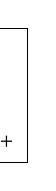
\begin{tikzpicture}[trim axis left, trim axis right]

\begin{axis}[%
width=\figurewidth,
height=\figureheight,
at={(0\figurewidth,0\figureheight)},
scale only axis,
every outer x axis line/.append style={black},
every x tick label/.append style={font=\color{black}},
xmin=9.5,
xmax=16,
xlabel={Time (h)},
every outer y axis line/.append style={black},
every y tick label/.append style={font=\color{black}},
ymin=-0.5,
ymax=0.5,
ylabel={Normalized Book Value},
axis background/.style={fill=white},
axis x line*=bottom,
axis y line*=left,
legend style={legend cell align=left,align=left,draw=black,font=\footnotesize, at={(0.98,0.02)},anchor=south east}
]
\addplot [color=black,solid]
  table[row sep=crcr]{%
9.50027777777778	0\\
9.50583333333333	0.00105999307347537\\
9.51138888888889	0.00126463670613708\\
9.51694444444444	0.0014710789527097\\
9.5225	0.00151689780736874\\
9.52805555555556	0.00149652797926958\\
9.53361111111111	0.00148483188711168\\
9.53916666666667	0.00152501863956633\\
9.54472222222222	0.00150924941436914\\
9.55027777777778	0.00160834385371911\\
9.55583333333333	0.00161875774764231\\
9.56138888888889	0.0016672176274648\\
9.56694444444444	0.00175485635065264\\
9.5725	0.00176020050243531\\
9.57805555555555	0.00170763054549306\\
9.58361111111111	0.00167134500142474\\
9.58916666666667	0.0017721366139396\\
9.59472222222222	0.00185907156763565\\
9.60027777777778	0.00184917937952034\\
9.60583333333333	0.00189357613081764\\
9.61138888888889	0.00183903292416376\\
9.61694444444444	0.0018522762452271\\
9.6225	0.00181121723226063\\
9.62805555555556	0.00180212756271358\\
9.63361111111111	0.00183227391439766\\
9.63916666666667	0.00188944150781811\\
9.64472222222222	0.00186503726533194\\
9.65027777777778	0.00185847494679758\\
9.65583333333333	0.00181317201415143\\
9.66138888888889	0.00185906265466174\\
9.66694444444444	0.00186278941915763\\
9.6725	0.0018675986607346\\
9.67805555555555	0.0017931228867325\\
9.68361111111111	0.00169981408696285\\
9.68916666666667	0.00178604340739996\\
9.69472222222222	0.00181589163250306\\
9.70027777777778	0.00181181573353362\\
9.70583333333333	0.00184413598584876\\
9.71138888888889	0.0018074021111889\\
9.71694444444444	0.00184153917105911\\
9.7225	0.00192420707323793\\
9.72805555555555	0.00189979225749104\\
9.73361111111111	0.00195766600710168\\
9.73916666666667	0.00197251590379799\\
9.74472222222222	0.00198186485455043\\
9.75027777777778	0.00194105760790375\\
9.75583333333333	0.00203102227323737\\
9.76138888888889	0.00203391021327448\\
9.76694444444444	0.00197902655597604\\
9.7725	0.0019643085226495\\
9.77805555555556	0.00197891608097978\\
9.78361111111111	0.00199649701684934\\
9.78916666666667	0.00194559352495127\\
9.79472222222222	0.00198152560386577\\
9.80027777777778	0.00203308329773577\\
9.80583333333333	0.00204709972937844\\
9.81138888888889	0.00209751080152953\\
9.81694444444444	0.00208797868607791\\
9.8225	0.00209748215542316\\
9.82805555555555	0.00214691274188383\\
9.83361111111111	0.00221530638153289\\
9.83916666666667	0.00219936513780494\\
9.84472222222222	0.00227671717837108\\
9.85027777777778	0.0022269422182366\\
9.85583333333333	0.00227225831762823\\
9.86138888888889	0.00223088322838572\\
9.86694444444444	0.00225985375521942\\
9.8725	0.00228955197353198\\
9.87805555555556	0.00230584803852119\\
9.88361111111111	0.00226322437916937\\
9.88916666666667	0.00223454173664828\\
9.89472222222222	0.00220013832873422\\
9.90027777777778	0.00224952911763321\\
9.90583333333333	0.00221624849200541\\
9.91138888888889	0.00218752693630697\\
9.91694444444444	0.00215618099587367\\
9.9225	0.00216875048805343\\
9.92805555555555	0.00213924352779804\\
9.93361111111111	0.0022273420642267\\
9.93916666666667	0.00223249257703584\\
9.94472222222222	0.0022640389936357\\
9.95027777777778	0.00228848626747813\\
9.95583333333333	0.00232868767119654\\
9.96138888888889	0.00232968973792169\\
9.96694444444444	0.00234378559237869\\
9.9725	0.00234627155512301\\
9.97805555555555	0.00231574695329484\\
9.98361111111111	0.00231455727858343\\
9.98916666666667	0.00229695448770473\\
9.99472222222222	0.0022936062326222\\
10.0002777777778	0.00230237886785778\\
10.0058333333333	0.00226339760045335\\
10.0113888888889	0.00218195034868862\\
10.0169444444444	0.00217348997176559\\
10.0225	0.00221162316220735\\
10.0280555555556	0.00221336334698496\\
10.0336111111111	0.00217946671354086\\
10.0391666666667	0.00226015813491021\\
10.0447222222222	0.00224407886131983\\
10.0502777777778	0.00224923653235831\\
10.0558333333333	0.00223784589614917\\
10.0613888888889	0.00222329201292037\\
10.0669444444444	0.00221431401691485\\
10.0725	0.00219412207082614\\
10.0780555555556	0.0022040956365712\\
10.0836111111111	0.00221288642080975\\
10.0891666666667	0.00218141542318695\\
10.0947222222222	0.00218567162967642\\
10.1002777777778	0.00215441281613282\\
10.1058333333333	0.002119808359206\\
10.1113888888889	0.0021357327682181\\
10.1169444444444	0.00219231184378188\\
10.1225	0.00217239916816192\\
10.1280555555556	0.00218798344423954\\
10.1336111111111	0.0021677578632322\\
10.1391666666667	0.00211263396816852\\
10.1447222222222	0.00212326124691731\\
10.1502777777778	0.00213196026230067\\
10.1558333333333	0.00209138812526466\\
10.1613888888889	0.00210267342743919\\
10.1669444444444	0.00207578662099794\\
10.1725	0.00201769967449583\\
10.1780555555556	0.00198887725375907\\
10.1836111111111	0.00204293076955464\\
10.1891666666667	0.00204381747309923\\
10.1947222222222	0.00201764269698979\\
10.2002777777778	0.00201222626301134\\
10.2058333333333	0.00198767185379234\\
10.2113888888889	0.00199723897658699\\
10.2169444444444	0.00202084961019611\\
10.2225	0.00205856027064732\\
10.2280555555556	0.0020092509281735\\
10.2336111111111	0.00200094277996032\\
10.2391666666667	0.0019733893240792\\
10.2447222222222	0.00195966675217618\\
10.2502777777778	0.00193877656580721\\
10.2558333333333	0.00195947766627702\\
10.2613888888889	0.00201144452229984\\
10.2669444444444	0.00197645953372105\\
10.2725	0.00198010698465678\\
10.2780555555556	0.00200461419424491\\
10.2836111111111	0.00203889118168221\\
10.2891666666667	0.00208235985934846\\
10.2947222222222	0.00209533540074114\\
10.3002777777778	0.00207842508206224\\
10.3058333333333	0.00200932945475185\\
10.3113888888889	0.00199336974606967\\
10.3169444444444	0.00199678700386507\\
10.3225	0.00199495800802785\\
10.3280555555556	0.00198130993517442\\
10.3336111111111	0.00198794013604209\\
10.3391666666667	0.00198940914337453\\
10.3447222222222	0.00201228218040916\\
10.3502777777778	0.00203169410433013\\
10.3558333333333	0.00201382208974055\\
10.3613888888889	0.00199261712497001\\
10.3669444444444	0.0019794860963307\\
10.3725	0.00196823194848372\\
10.3780555555556	0.00199190495740065\\
10.3836111111111	0.00196638675749039\\
10.3891666666667	0.0019253323092765\\
10.3947222222222	0.00189405354984307\\
10.4002777777778	0.00190792266091555\\
10.4058333333333	0.00194880882345361\\
10.4113888888889	0.00189481961071314\\
10.4169444444444	0.00196086932657757\\
10.4225	0.00196289483743972\\
10.4280555555556	0.0018891778349206\\
10.4336111111111	0.00185167657057694\\
10.4391666666667	0.00181652659613496\\
10.4447222222222	0.00181542977895965\\
10.4502777777778	0.00182694989582077\\
10.4558333333333	0.00184645931742522\\
10.4613888888889	0.00184342293372142\\
10.4669444444444	0.00184519512731707\\
10.4725	0.00186314761361239\\
10.4780555555556	0.00186122148155965\\
10.4836111111111	0.00185290727218068\\
10.4891666666667	0.00179998847716489\\
10.4947222222222	0.00179812577762273\\
10.5002777777778	0.0017764503842812\\
10.5058333333333	0.00177292566272924\\
10.5113888888889	0.00174190970788635\\
10.5169444444444	0.00175321924533089\\
10.5225	0.00173214008597178\\
10.5280555555556	0.00173052734020773\\
10.5336111111111	0.00173341109109026\\
10.5391666666667	0.00179055747063916\\
10.5447222222222	0.00180667328269135\\
10.5502777777778	0.00177777102830934\\
10.5558333333333	0.00177767703924503\\
10.5613888888889	0.00174292376469909\\
10.5669444444444	0.00173889278029815\\
10.5725	0.00174984265930989\\
10.5780555555556	0.00178085723544052\\
10.5836111111111	0.00178016451832153\\
10.5891666666667	0.00181192482409243\\
10.5947222222222	0.00181045441170014\\
10.6002777777778	0.00176679113736999\\
10.6058333333333	0.00181608267309707\\
10.6113888888889	0.00176693620926405\\
10.6169444444444	0.00172798736509483\\
10.6225	0.00172945225622922\\
10.6280555555556	0.0016967953215008\\
10.6336111111111	0.00170825691347765\\
10.6391666666667	0.00171495116278741\\
10.6447222222222	0.00168574855243464\\
10.6502777777778	0.00170043011891474\\
10.6558333333333	0.00172576452760098\\
10.6613888888889	0.00166932541275489\\
10.6669444444444	0.00167613801820821\\
10.6725	0.00169145816554583\\
10.6780555555556	0.00167750176006032\\
10.6836111111111	0.0017051951872582\\
10.6891666666667	0.00172376633623128\\
10.6947222222222	0.00174866053597511\\
10.7002777777778	0.00171804652887908\\
10.7058333333333	0.00171458717578643\\
10.7113888888889	0.00165265840328543\\
10.7169444444444	0.00163600775607708\\
10.7225	0.0016773796586067\\
10.7280555555556	0.00167730651132936\\
10.7336111111111	0.00170585763939113\\
10.7391666666667	0.00173863280674413\\
10.7447222222222	0.00175590586984775\\
10.7502777777778	0.00178222860458899\\
10.7558333333333	0.00175345113300152\\
10.7613888888889	0.00174395749294542\\
10.7669444444444	0.00172416022497845\\
10.7725	0.00174548402616037\\
10.7780555555556	0.00176909549717652\\
10.7836111111111	0.00171900237118106\\
10.7891666666667	0.00174109317819471\\
10.7947222222222	0.00171786641564431\\
10.8002777777778	0.00168976241625596\\
10.8058333333333	0.00172659690415511\\
10.8113888888889	0.00170520182419365\\
10.8169444444444	0.00167346698135096\\
10.8225	0.00168736890776877\\
10.8280555555556	0.00169904192676373\\
10.8336111111111	0.00176251212593947\\
10.8391666666667	0.00175615956700836\\
10.8447222222222	0.00173338772174914\\
10.8502777777778	0.00168216290376111\\
10.8558333333333	0.00169345860723635\\
10.8613888888889	0.00171514246477433\\
10.8669444444444	0.00172193056909942\\
10.8725	0.00170087650275019\\
10.8780555555556	0.00170800789011483\\
10.8836111111111	0.00173004701257784\\
10.8891666666667	0.00174171782016219\\
10.8947222222222	0.00174164019641654\\
10.9002777777778	0.00172737484804752\\
10.9058333333333	0.00173340411221057\\
10.9113888888889	0.00169572259462947\\
10.9169444444444	0.00174942412686674\\
10.9225	0.00175344947310396\\
10.9280555555556	0.0017681902857638\\
10.9336111111111	0.00175551818162312\\
10.9391666666667	0.00177480057795454\\
10.9447222222222	0.00180269975796765\\
10.9502777777778	0.0018051042596916\\
10.9558333333333	0.00177846860336595\\
10.9613888888889	0.00178603963697532\\
10.9669444444444	0.00177179886508139\\
10.9725	0.00175177091135859\\
10.9780555555556	0.00175124610206012\\
10.9836111111111	0.00178616935095466\\
10.9891666666667	0.00178503121778673\\
10.9947222222222	0.00179067470801209\\
11.0002777777778	0.00178111688635263\\
11.0058333333333	0.00179176786352153\\
11.0113888888889	0.00175614318945372\\
11.0169444444444	0.00172551644389984\\
11.0225	0.00172272633431603\\
11.0280555555556	0.00172190077176371\\
11.0336111111111	0.00170317971614842\\
11.0391666666667	0.0016925570981956\\
11.0447222222222	0.00172138852552783\\
11.0502777777778	0.00175383710025434\\
11.0558333333333	0.00177246476571491\\
11.0613888888889	0.00177933421555765\\
11.0669444444444	0.00180726084527416\\
11.0725	0.00180814612677271\\
11.0780555555556	0.00177477503518375\\
11.0836111111111	0.00173940177489329\\
11.0891666666667	0.0017504950408338\\
11.0947222222222	0.00176362599410851\\
11.1002777777778	0.00180911493167679\\
11.1058333333333	0.00180091576741948\\
11.1113888888889	0.00179318218085411\\
11.1169444444444	0.00183262481356539\\
11.1225	0.00185505875830416\\
11.1280555555556	0.00181805716090278\\
11.1336111111111	0.00179562838844194\\
11.1391666666667	0.00179582140366286\\
11.1447222222222	0.00179194010302219\\
11.1502777777778	0.00176465380609603\\
11.1558333333333	0.00179020084276638\\
11.1613888888889	0.00177275255654696\\
11.1669444444444	0.00179217663239295\\
11.1725	0.00180099989576887\\
11.1780555555556	0.00183278624630168\\
11.1836111111111	0.0018143838458462\\
11.1891666666667	0.00183209202162349\\
11.1947222222222	0.00183312035822847\\
11.2002777777778	0.00178229054369594\\
11.2058333333333	0.00181091140155987\\
11.2113888888889	0.00185252162146421\\
11.2169444444444	0.00184689192709908\\
11.2225	0.00185477153041491\\
11.2280555555556	0.00184500414069122\\
11.2336111111111	0.00186545758290158\\
11.2391666666667	0.00187907752291783\\
11.2447222222222	0.00187339634788164\\
11.2502777777778	0.00187708131480013\\
11.2558333333333	0.00194631150760149\\
11.2613888888889	0.00190690311284136\\
11.2669444444444	0.00190966717926844\\
11.2725	0.00202537898797805\\
11.2780555555556	0.00203794831687798\\
11.2836111111111	0.00199913622361936\\
11.2891666666667	0.00202168717384921\\
11.2947222222222	0.00200595264883896\\
11.3002777777778	0.00201656112178772\\
11.3058333333333	0.00195721405883909\\
11.3113888888889	0.00193783341410558\\
11.3169444444444	0.00191472444342256\\
11.3225	0.00196228361721706\\
11.3280555555556	0.00192835627514909\\
11.3336111111111	0.00195150577718062\\
11.3391666666667	0.00197616191478711\\
11.3447222222222	0.00195745598500041\\
11.3502777777778	0.0019699833774276\\
11.3558333333333	0.00195541721444226\\
11.3613888888889	0.00192953020285636\\
11.3669444444444	0.00192726295151946\\
11.3725	0.00192196869573036\\
11.3780555555556	0.00189956550686343\\
11.3836111111111	0.00187039494856256\\
11.3891666666667	0.00184261568313859\\
11.3947222222222	0.00179928855051803\\
11.4002777777778	0.00176431068817595\\
11.4058333333333	0.00175041956626032\\
11.4113888888889	0.0017799292881493\\
11.4169444444444	0.00177163567716465\\
11.4225	0.00180405340973122\\
11.4280555555556	0.00180278543006929\\
11.4336111111111	0.00182587204004059\\
11.4391666666667	0.00181657022230008\\
11.4447222222222	0.00178359880915457\\
11.4502777777778	0.00176850820004359\\
11.4558333333333	0.00175502645279013\\
11.4613888888889	0.00172563905064282\\
11.4669444444444	0.00174081439897789\\
11.4725	0.00175122634975255\\
11.4780555555556	0.00175986096532554\\
11.4836111111111	0.00174509264980283\\
11.4891666666667	0.00170360516095847\\
11.4947222222222	0.00165042315258024\\
11.5002777777778	0.00164740653961615\\
11.5058333333333	0.0016644533753325\\
11.5113888888889	0.0016942343685753\\
11.5169444444444	0.00169464288989074\\
11.5225	0.00164868609965785\\
11.5280555555556	0.00166530811532772\\
11.5336111111111	0.00168491358474565\\
11.5391666666667	0.00172719796679743\\
11.5447222222222	0.00172544611238767\\
11.5502777777778	0.00174006981384989\\
11.5558333333333	0.00175428749851014\\
11.5613888888889	0.00174574348623779\\
11.5669444444444	0.00174791632075699\\
11.5725	0.00173710844501085\\
11.5780555555556	0.00172497301647745\\
11.5836111111111	0.00175369684384319\\
11.5891666666667	0.00177936270769941\\
11.5947222222222	0.00179193274287326\\
11.6002777777778	0.00180110032814751\\
11.6058333333333	0.00184257260547072\\
11.6113888888889	0.00184127000314915\\
11.6169444444444	0.00188229640372595\\
11.6225	0.00186211629176092\\
11.6280555555556	0.00188864332791328\\
11.6336111111111	0.00188785668260305\\
11.6391666666667	0.00188214679058651\\
11.6447222222222	0.00186149315869533\\
11.6502777777778	0.00186694483628358\\
11.6558333333333	0.00188593126444148\\
11.6613888888889	0.00188082078332275\\
11.6669444444444	0.00187561583665841\\
11.6725	0.00187844035642648\\
11.6780555555556	0.00182348562952717\\
11.6836111111111	0.00181325567926804\\
11.6891666666667	0.00179925998024055\\
11.6947222222222	0.00179881559859196\\
11.7002777777778	0.00178325571635551\\
11.7058333333333	0.00178802739085704\\
11.7113888888889	0.00180226363035607\\
11.7169444444444	0.0017862878065531\\
11.7225	0.00179228427610378\\
11.7280555555556	0.00177491783833883\\
11.7336111111111	0.0017833186876921\\
11.7391666666667	0.00180132681384682\\
11.7447222222222	0.00180293967415857\\
11.7502777777778	0.00181121666570827\\
11.7558333333333	0.00184880880965266\\
11.7613888888889	0.00187072141892508\\
11.7669444444444	0.0018917797912632\\
11.7725	0.00189938178989402\\
11.7780555555556	0.00187973475041736\\
11.7836111111111	0.00186294633337458\\
11.7891666666667	0.0018775148697403\\
11.7947222222222	0.00186820872282745\\
11.8002777777778	0.00188168180658366\\
11.8058333333333	0.0018635616786844\\
11.8113888888889	0.00186193584877148\\
11.8169444444444	0.0018413848533585\\
11.8225	0.00182278113500511\\
11.8280555555556	0.00182231789755405\\
11.8336111111111	0.00185836290000974\\
11.8391666666667	0.0018353453045532\\
11.8447222222222	0.00183112573668343\\
11.8502777777778	0.00183169680922091\\
11.8558333333333	0.0018437754562135\\
11.8613888888889	0.00181337871504539\\
11.8669444444444	0.00183311876177505\\
11.8725	0.00183849494388055\\
11.8780555555556	0.00181024044024602\\
11.8836111111111	0.00179406307644059\\
11.8891666666667	0.00184060324021873\\
11.8947222222222	0.00184371903773672\\
11.9002777777778	0.00182930334911169\\
11.9058333333333	0.00184606958944578\\
11.9113888888889	0.00182902518397388\\
11.9169444444444	0.00184044068222988\\
11.9225	0.00186978793358206\\
11.9280555555556	0.00188482082352115\\
11.9336111111111	0.00189754860952673\\
11.9391666666667	0.00188025669302649\\
11.9447222222222	0.00189230627078674\\
11.9502777777778	0.00190028553455734\\
11.9558333333333	0.0019053742860029\\
11.9613888888889	0.00192135937727667\\
11.9669444444444	0.00192603026102578\\
11.9725	0.00191648312390313\\
11.9780555555556	0.00194816237835949\\
11.9836111111111	0.00193794573839701\\
11.9891666666667	0.00195513386872515\\
11.9947222222222	0.00195937345385588\\
12.0002777777778	0.00192689184973815\\
12.0058333333333	0.00192312043747345\\
12.0113888888889	0.00192685231265433\\
12.0169444444444	0.00193162628099031\\
12.0225	0.0019391799343893\\
12.0280555555556	0.00190095891953357\\
12.0336111111111	0.00189353568020056\\
12.0391666666667	0.00187720276088799\\
12.0447222222222	0.00187022739345721\\
12.0502777777778	0.00185414848349841\\
12.0558333333333	0.00185188884305831\\
12.0613888888889	0.00182432099864371\\
12.0669444444444	0.00181810488636569\\
12.0725	0.00183876011396289\\
12.0780555555556	0.00183145949407693\\
12.0836111111111	0.00184317736510575\\
12.0891666666667	0.0018320999235113\\
12.0947222222222	0.00182942353016724\\
12.1002777777778	0.00183040925991218\\
12.1058333333333	0.00184384727007592\\
12.1113888888889	0.00186135529782727\\
12.1169444444444	0.00191468274166562\\
12.1225	0.00191307953201747\\
12.1280555555556	0.00189770684757828\\
12.1336111111111	0.00191394219756047\\
12.1391666666667	0.00190900093222335\\
12.1447222222222	0.00190678813161838\\
12.1502777777778	0.00192596715799342\\
12.1558333333333	0.00188984972931472\\
12.1613888888889	0.00189282316390949\\
12.1669444444444	0.00188458696689353\\
12.1725	0.00186102312968184\\
12.1780555555556	0.00183509167822948\\
12.1836111111111	0.00182421720944981\\
12.1891666666667	0.0018299457033617\\
12.1947222222222	0.00184861425483596\\
12.2002777777778	0.00183320841512957\\
12.2058333333333	0.00184564250681762\\
12.2113888888889	0.0018622636647565\\
12.2169444444444	0.00184344647248968\\
12.2225	0.00187752867577484\\
12.2280555555556	0.00189758918113547\\
12.2336111111111	0.00191392869808382\\
12.2391666666667	0.00192995706059085\\
12.2447222222222	0.00193291430937048\\
12.2502777777778	0.00193702121007711\\
12.2558333333333	0.00194234544224448\\
12.2613888888889	0.00192942028383158\\
12.2669444444444	0.00193191048407537\\
12.2725	0.00193644627579093\\
12.2780555555556	0.00192583602599772\\
12.2836111111111	0.00193835766957129\\
12.2891666666667	0.00190159934014789\\
12.2947222222222	0.00190650160337569\\
12.3002777777778	0.0019330076208699\\
12.3058333333333	0.00193515640140474\\
12.3113888888889	0.00194596504786992\\
12.3169444444444	0.00196720265780481\\
12.3225	0.00197132851627702\\
12.3280555555556	0.00197195775576486\\
12.3336111111111	0.00196265022749054\\
12.3391666666667	0.00196308428988523\\
12.3447222222222	0.0019673820504984\\
12.3502777777778	0.00195935098501021\\
12.3558333333333	0.00195848870816318\\
12.3613888888889	0.0019668025338504\\
12.3669444444444	0.0019889789922094\\
12.3725	0.00201780485594205\\
12.3780555555556	0.00200195961170846\\
12.3836111111111	0.00203124194291004\\
12.3891666666667	0.00205351943117416\\
12.3947222222222	0.00204744642626253\\
12.4002777777778	0.00205436599639541\\
12.4058333333333	0.00205372316717178\\
12.4113888888889	0.00205313603047075\\
12.4169444444444	0.00204451899947999\\
12.4225	0.00201490015541861\\
12.4280555555556	0.00203394994576889\\
12.4336111111111	0.00199487985192581\\
12.4391666666667	0.00197729722241147\\
12.4447222222222	0.00199717968600988\\
12.4502777777778	0.00199023519067421\\
12.4558333333333	0.00196644468202689\\
12.4613888888889	0.00195961274662904\\
12.4669444444444	0.00194828217905418\\
12.4725	0.00194844910165193\\
12.4780555555556	0.00191990254196051\\
12.4836111111111	0.00192016546887319\\
12.4891666666667	0.00194637856118951\\
12.4947222222222	0.0019693744938778\\
12.5002777777778	0.00195841718066592\\
12.5058333333333	0.00196414291210512\\
12.5113888888889	0.00194173138577725\\
12.5169444444444	0.00193408180979815\\
12.5225	0.00192085070483827\\
12.5280555555556	0.00190771858663474\\
12.5336111111111	0.00192563579605154\\
12.5391666666667	0.0019107737851729\\
12.5447222222222	0.00190376019294103\\
12.5502777777778	0.00193782666200493\\
12.5558333333333	0.00194928618165657\\
12.5613888888889	0.00194780528839411\\
12.5669444444444	0.00194943272289505\\
12.5725	0.00193848483162951\\
12.5780555555556	0.00194709825435169\\
12.5836111111111	0.00195455454879356\\
12.5891666666667	0.00197779139081256\\
12.5947222222222	0.00199187480500829\\
12.6002777777778	0.00200286456668031\\
12.6058333333333	0.00200888264165\\
12.6113888888889	0.00201681718212066\\
12.6169444444444	0.00201142716762392\\
12.6225	0.00203341622279707\\
12.6280555555556	0.00204845301374212\\
12.6336111111111	0.00204832756982154\\
12.6391666666667	0.00205704097359916\\
12.6447222222222	0.00207866756524977\\
12.6502777777778	0.00209719550885046\\
12.6558333333333	0.00208409931642572\\
12.6613888888889	0.00207602990924438\\
12.6669444444444	0.00205824044695846\\
12.6725	0.00205240056913114\\
12.6780555555556	0.00206330749212724\\
12.6836111111111	0.00207292530013237\\
12.6891666666667	0.00209741780900696\\
12.6947222222222	0.00209851853313925\\
12.7002777777778	0.00209096742605719\\
12.7058333333333	0.00208883695766615\\
12.7113888888889	0.0021006680377158\\
12.7169444444444	0.00210815286397703\\
12.7225	0.00211652189083855\\
12.7280555555556	0.00213312614891104\\
12.7336111111111	0.00215587152382435\\
12.7391666666667	0.00216723877330405\\
12.7447222222222	0.00217144897454613\\
12.7502777777778	0.00218901689338424\\
12.7558333333333	0.00219045377935756\\
12.7613888888889	0.00218307405724749\\
12.7669444444444	0.00219152005577739\\
12.7725	0.0021803299286427\\
12.7780555555556	0.00217734609004161\\
12.7836111111111	0.00214498668314\\
12.7891666666667	0.00216672042223665\\
12.7947222222222	0.00217936120802631\\
12.8002777777778	0.00216218767381759\\
12.8058333333333	0.00216406220895959\\
12.8113888888889	0.0021372288994248\\
12.8169444444444	0.00212575450036412\\
12.8225	0.00212793069924144\\
12.8280555555556	0.00214608525449234\\
12.8336111111111	0.00215389963615942\\
12.8391666666667	0.00215249134133355\\
12.8447222222222	0.00212389882094444\\
12.8502777777778	0.00213188662032571\\
12.8558333333333	0.00213081802924187\\
12.8613888888889	0.00214749309154794\\
12.8669444444444	0.00217304657586692\\
12.8725	0.00216775226911459\\
12.8780555555556	0.00215424981798695\\
12.8836111111111	0.00213760626797899\\
12.8891666666667	0.00215288807578617\\
12.8947222222222	0.00214296417479853\\
12.9002777777778	0.0021394735484821\\
12.9058333333333	0.00215876533842141\\
12.9113888888889	0.00217135289313086\\
12.9169444444444	0.00218562871674988\\
12.9225	0.00219625808302881\\
12.9280555555556	0.002225061414036\\
12.9336111111111	0.00222957481676178\\
12.9391666666667	0.00222246509101787\\
12.9447222222222	0.00221781582603686\\
12.9502777777778	0.00222892727047985\\
12.9558333333333	0.00222733251899165\\
12.9613888888889	0.00222149549419903\\
12.9669444444444	0.0022624815811414\\
12.9725	0.00227113188711225\\
12.9780555555556	0.00223355810519732\\
12.9836111111111	0.00223044284938223\\
12.9891666666667	0.00221925643619758\\
12.9947222222222	0.00222579225545294\\
13.0002777777778	0.00219803851331757\\
13.0058333333333	0.0022213627467742\\
13.0113888888889	0.00224471080013866\\
13.0169444444444	0.0022457316733151\\
13.0225	0.00224967851957913\\
13.0280555555556	0.00223317517529154\\
13.0336111111111	0.00225069186075255\\
13.0391666666667	0.00222927745729384\\
13.0447222222222	0.0022192696840222\\
13.0502777777778	0.00222921536491283\\
13.0558333333333	0.00221044086661104\\
13.0613888888889	0.00222850868720137\\
13.0669444444444	0.00222514544535413\\
13.0725	0.0022360877348937\\
13.0780555555556	0.00223557426027221\\
13.0836111111111	0.0022349826488024\\
13.0891666666667	0.00224717151972209\\
13.0947222222222	0.0022534026755523\\
13.1002777777778	0.00225327861667024\\
13.1058333333333	0.0022421303485336\\
13.1113888888889	0.00223447148241274\\
13.1169444444444	0.00226021430621226\\
13.1225	0.00227226214364418\\
13.1280555555556	0.00229718795896017\\
13.1336111111111	0.00229326272221342\\
13.1391666666667	0.00228908208957668\\
13.1447222222222	0.00227214245429641\\
13.1502777777778	0.00226287322866803\\
13.1558333333333	0.00220911557078618\\
13.1613888888889	0.00218068571673924\\
13.1669444444444	0.00213524981110158\\
13.1725	0.00215345701593583\\
13.1780555555556	0.00215132133651963\\
13.1836111111111	0.00216211245737519\\
13.1891666666667	0.00219076515961003\\
13.1947222222222	0.00218171599200256\\
13.2002777777778	0.00218171503174025\\
13.2058333333333	0.00216936127405387\\
13.2113888888889	0.00217720049376724\\
13.2169444444444	0.00217182669914173\\
13.2225	0.00217186694321048\\
13.2280555555556	0.00216782101335955\\
13.2336111111111	0.00217972255169663\\
13.2391666666667	0.00215820167384195\\
13.2447222222222	0.00214107413587494\\
13.2502777777778	0.00211299721524649\\
13.2558333333333	0.00209889624589388\\
13.2613888888889	0.0021178264585926\\
13.2669444444444	0.00211687949812878\\
13.2725	0.00212954334169058\\
13.2780555555556	0.00214806374177368\\
13.2836111111111	0.00210373114449336\\
13.2891666666667	0.00211579399299633\\
13.2947222222222	0.00212230665916602\\
13.3002777777778	0.00210377556192576\\
13.3058333333333	0.00209956036946735\\
13.3113888888889	0.00211286955425205\\
13.3169444444444	0.00211450445349115\\
13.3225	0.00213627609924627\\
13.3280555555556	0.0021267209483935\\
13.3336111111111	0.00214808115577525\\
13.3391666666667	0.00216015718974916\\
13.3447222222222	0.00217405776732504\\
13.3502777777778	0.00216190475539757\\
13.3558333333333	0.00214163274956092\\
13.3613888888889	0.00212466130809519\\
13.3669444444444	0.00210350862893827\\
13.3725	0.0021141133960656\\
13.3780555555556	0.002100527474034\\
13.3836111111111	0.00212204111821079\\
13.3891666666667	0.00212895376749933\\
13.3947222222222	0.00210997300972737\\
13.4002777777778	0.00212422479573982\\
13.4058333333333	0.00212759491515402\\
13.4113888888889	0.00214337384640562\\
13.4169444444444	0.00214930440556671\\
13.4225	0.00216376346451264\\
13.4280555555556	0.00216948081448409\\
13.4336111111111	0.00217591182318544\\
13.4391666666667	0.00219374590942278\\
13.4447222222222	0.00219055348008612\\
13.4502777777778	0.00215250216992247\\
13.4558333333333	0.00214311321417759\\
13.4613888888889	0.00216806706435091\\
13.4669444444444	0.00214476954925935\\
13.4725	0.00214352857871702\\
13.4780555555556	0.0021685928469517\\
13.4836111111111	0.00220183398215235\\
13.4891666666667	0.00219260904990781\\
13.4947222222222	0.0021621794125708\\
13.5002777777778	0.00215340884792692\\
13.5058333333333	0.00215262028614482\\
13.5113888888889	0.00212496049223199\\
13.5169444444444	0.00212769325650308\\
13.5225	0.00211289245483104\\
13.5280555555556	0.00210587208553492\\
13.5336111111111	0.00210008638490344\\
13.5391666666667	0.00209693389188859\\
13.5447222222222	0.00211396196992575\\
13.5502777777778	0.00214564327023714\\
13.5558333333333	0.00213434924088474\\
13.5613888888889	0.00214876647375473\\
13.5669444444444	0.00217273738648438\\
13.5725	0.00217512631609096\\
13.5780555555556	0.00218615649148557\\
13.5836111111111	0.00221225645810108\\
13.5891666666667	0.00218841821374993\\
13.5947222222222	0.00217654587072924\\
13.6002777777778	0.00219432342268799\\
13.6058333333333	0.00221404739075926\\
13.6113888888889	0.00222177761225417\\
13.6169444444444	0.00223245059781618\\
13.6225	0.00225033043723188\\
13.6280555555556	0.00225025358884623\\
13.6336111111111	0.00222755680023834\\
13.6391666666667	0.00223363744045502\\
13.6447222222222	0.00225762614057445\\
13.6502777777778	0.00223913688863941\\
13.6558333333333	0.00222433210331729\\
13.6613888888889	0.00222582594356902\\
13.6669444444444	0.0022332708464492\\
13.6725	0.00226697353851213\\
13.6780555555556	0.00226228143320872\\
13.6836111111111	0.00227365512744271\\
13.6891666666667	0.00224103116946583\\
13.6947222222222	0.00227533691338611\\
13.7002777777778	0.00223215021966361\\
13.7058333333333	0.00224951234056614\\
13.7113888888889	0.00226682253274468\\
13.7169444444444	0.00226939161483264\\
13.7225	0.00226149482976745\\
13.7280555555556	0.00226760736326703\\
13.7336111111111	0.00228788622306775\\
13.7391666666667	0.00230927656428803\\
13.7447222222222	0.0023196389948954\\
13.7502777777778	0.00235260536151571\\
13.7558333333333	0.00233341340776727\\
13.7613888888889	0.00233107174104141\\
13.7669444444444	0.00231962340888625\\
13.7725	0.00233009068903356\\
13.7780555555556	0.00229785718771414\\
13.7836111111111	0.00227903341520808\\
13.7891666666667	0.00229367953260495\\
13.7947222222222	0.00231591541890186\\
13.8002777777778	0.00231014386542916\\
13.8058333333333	0.00230317815082737\\
13.8113888888889	0.00228908658789018\\
13.8169444444444	0.00227832726439647\\
13.8225	0.00230246069498752\\
13.8280555555556	0.00230856910154431\\
13.8336111111111	0.0022811995881995\\
13.8391666666667	0.00226283407959205\\
13.8447222222222	0.00226252681012995\\
13.8502777777778	0.0022730487500735\\
13.8558333333333	0.00228655948356438\\
13.8613888888889	0.00227387568247006\\
13.8669444444444	0.00226109143658837\\
13.8725	0.00222749281439816\\
13.8780555555556	0.00221453238469649\\
13.8836111111111	0.00223091270253661\\
13.8891666666667	0.00226642234332575\\
13.8947222222222	0.00226464175578633\\
13.9002777777778	0.00228377896052034\\
13.9058333333333	0.00227378659040856\\
13.9113888888889	0.0022689784820169\\
13.9169444444444	0.00226359011853816\\
13.9225	0.00229154953099808\\
13.9280555555556	0.00229456042011456\\
13.9336111111111	0.00231199118037795\\
13.9391666666667	0.0023051457203962\\
13.9447222222222	0.00230830423907991\\
13.9502777777778	0.00233837385703106\\
13.9558333333333	0.00234144514335943\\
13.9613888888889	0.00231132286614621\\
13.9669444444444	0.00231591128734832\\
13.9725	0.00229609323921043\\
13.9780555555556	0.00230383664768663\\
13.9836111111111	0.00235196550235517\\
13.9891666666667	0.00237052402091442\\
13.9947222222222	0.00236475739755959\\
14.0002777777778	0.00235815867682398\\
14.0058333333333	0.00237014106978184\\
14.0113888888889	0.00236601864304298\\
14.0169444444444	0.00238485104686137\\
14.0225	0.00237444040944568\\
14.0280555555556	0.00238420121514471\\
14.0336111111111	0.00234140992236154\\
14.0391666666667	0.00234054695031527\\
14.0447222222222	0.00234226619218059\\
14.0502777777778	0.00236273684874577\\
14.0558333333333	0.00235320602015054\\
14.0613888888889	0.00235933295339308\\
14.0669444444444	0.00235652799958053\\
14.0725	0.00233184698475397\\
14.0780555555556	0.0023222285647575\\
14.0836111111111	0.00236992269441605\\
14.0891666666667	0.00241206534306659\\
14.0947222222222	0.00240077376497694\\
14.1002777777778	0.00239621492530806\\
14.1058333333333	0.00238231102521858\\
14.1113888888889	0.00243922025017396\\
14.1169444444444	0.00240885623667397\\
14.1225	0.0023955557113513\\
14.1280555555556	0.00239485469972811\\
14.1336111111111	0.00243001237741214\\
14.1391666666667	0.00241212251560108\\
14.1447222222222	0.00241467422829222\\
14.1502777777778	0.00239511220040445\\
14.1558333333333	0.00241708638713045\\
14.1613888888889	0.00237753874134117\\
14.1669444444444	0.00237100557681647\\
14.1725	0.00234599474459096\\
14.1780555555556	0.00236635593313506\\
14.1836111111111	0.00236509840441057\\
14.1891666666667	0.00233947035181536\\
14.1947222222222	0.0023221218225602\\
14.2002777777778	0.00232340987189628\\
14.2058333333333	0.0023427368907154\\
14.2113888888889	0.00235759761156928\\
14.2169444444444	0.00237226872377039\\
14.2225	0.00233560173231817\\
14.2280555555556	0.00233094205526974\\
14.2336111111111	0.00234311834897416\\
14.2391666666667	0.00231991051228309\\
14.2447222222222	0.00230419207916666\\
14.2502777777778	0.00228540567684554\\
14.2558333333333	0.00228595374816898\\
14.2613888888889	0.00227921916898666\\
14.2669444444444	0.00228487818059642\\
14.2725	0.00224242806530794\\
14.2780555555556	0.00226959191725995\\
14.2836111111111	0.00227149597177179\\
14.2891666666667	0.00228136163962622\\
14.2947222222222	0.00226870850869099\\
14.3002777777778	0.0022751685972966\\
14.3058333333333	0.00227158172249275\\
14.3113888888889	0.00229468600045335\\
14.3169444444444	0.00230818352105833\\
14.3225	0.00234086234273101\\
14.3280555555556	0.00235717096614407\\
14.3336111111111	0.00233252168096199\\
14.3391666666667	0.00236353553187318\\
14.3447222222222	0.00233642213528773\\
14.3502777777778	0.00234514564708288\\
14.3558333333333	0.00233451410404006\\
14.3613888888889	0.00232041410911532\\
14.3669444444444	0.00233538170613246\\
14.3725	0.00233360047160258\\
14.3780555555556	0.00232016414731762\\
14.3836111111111	0.00232468643904937\\
14.3891666666667	0.00236767668210636\\
14.3947222222222	0.00233573081330274\\
14.4002777777778	0.00234821051976319\\
14.4058333333333	0.00232011577511604\\
14.4113888888889	0.00232898611532995\\
14.4169444444444	0.00233142289985011\\
14.4225	0.00233349801336824\\
14.4280555555556	0.00231977496123204\\
14.4336111111111	0.00231754736925405\\
14.4391666666667	0.00232137249507747\\
14.4447222222222	0.00230533903727781\\
14.4502777777778	0.00234054558304075\\
14.4558333333333	0.00233404932730075\\
14.4613888888889	0.00233511755576821\\
14.4669444444444	0.00234349392936273\\
14.4725	0.00234237076390675\\
14.4780555555556	0.0023678873738322\\
14.4836111111111	0.00236102808497729\\
14.4891666666667	0.00234853364509013\\
14.4947222222222	0.00241556278859689\\
14.5002777777778	0.0024007099884642\\
14.5058333333333	0.00236865213182491\\
14.5113888888889	0.00239132108201079\\
14.5169444444444	0.00240335012745185\\
14.5225	0.00243184294877818\\
14.5280555555556	0.00240582568720926\\
14.5336111111111	0.00239509209054356\\
14.5391666666667	0.00239050941403596\\
14.5447222222222	0.00238558037246661\\
14.5502777777778	0.00235956451438546\\
14.5558333333333	0.0023670393262174\\
14.5613888888889	0.00236490280151558\\
14.5669444444444	0.00237747486089446\\
14.5725	0.00235670294349255\\
14.5780555555556	0.00235190600285917\\
14.5836111111111	0.00231912313769844\\
14.5891666666667	0.00233591363969698\\
14.5947222222222	0.00236028088615514\\
14.6002777777778	0.00235004276349593\\
14.6058333333333	0.00232432905019642\\
14.6113888888889	0.0023123013271793\\
14.6169444444444	0.00230627622775836\\
14.6225	0.00230186825215006\\
14.6280555555556	0.00227828235163785\\
14.6336111111111	0.00226271473676176\\
14.6391666666667	0.00224105294618915\\
14.6447222222222	0.00224247713128456\\
14.6502777777778	0.00225427939101519\\
14.6558333333333	0.00225203213929448\\
14.6613888888889	0.00227063782243886\\
14.6669444444444	0.00227551858040109\\
14.6725	0.00231139137823755\\
14.6780555555556	0.00233763771303663\\
14.6836111111111	0.00231427009452068\\
14.6891666666667	0.00234948214821573\\
14.6947222222222	0.00235958111340562\\
14.7002777777778	0.00236247447918125\\
14.7058333333333	0.00235636715342635\\
14.7113888888889	0.00235151604246941\\
14.7169444444444	0.00235247297773511\\
14.7225	0.00238167141646617\\
14.7280555555556	0.00238566279879482\\
14.7336111111111	0.00238184803568275\\
14.7391666666667	0.00237868982031908\\
14.7447222222222	0.00235862397555664\\
14.7502777777778	0.00237211802704529\\
14.7558333333333	0.00239943362740647\\
14.7613888888889	0.00238125773303133\\
14.7669444444444	0.00239188134374668\\
14.7725	0.0023787604467731\\
14.7780555555556	0.00234638892828243\\
14.7836111111111	0.00233455890960621\\
14.7891666666667	0.00233832753634489\\
14.7947222222222	0.00234143906738282\\
14.8002777777778	0.00235607539221827\\
14.8058333333333	0.00235064622252978\\
14.8113888888889	0.00236044138309288\\
14.8169444444444	0.00238751044578178\\
14.8225	0.00237340160430111\\
14.8280555555556	0.00235544799667919\\
14.8336111111111	0.00237094824476958\\
14.8391666666667	0.00238635680061505\\
14.8447222222222	0.00239744598644154\\
14.8502777777778	0.0023807481262228\\
14.8558333333333	0.00238381289978395\\
14.8613888888889	0.00236460035701769\\
14.8669444444444	0.00234028678818654\\
14.8725	0.00236175158005958\\
14.8780555555556	0.00235346129943648\\
14.8836111111111	0.00233466046705555\\
14.8891666666667	0.00230377758171207\\
14.8947222222222	0.00229697999706979\\
14.9002777777778	0.0023017956078919\\
14.9058333333333	0.00229592571651671\\
14.9113888888889	0.00230296252695306\\
14.9169444444444	0.00232450910680027\\
14.9225	0.00230487574331262\\
14.9280555555556	0.00231740766482114\\
14.9336111111111	0.0023077242062981\\
14.9391666666667	0.00231793290553339\\
14.9447222222222	0.00232130293844368\\
14.9502777777778	0.0022998552277782\\
14.9558333333333	0.00226040359165514\\
14.9613888888889	0.00226615306059408\\
14.9669444444444	0.0023108489108481\\
14.9725	0.00232434330535192\\
14.9780555555556	0.0023187519093939\\
14.9836111111111	0.0023334782175779\\
14.9891666666667	0.00233134023678483\\
14.9947222222222	0.00231536917194575\\
15.0002777777778	0.00231386048704274\\
15.0058333333333	0.00232235508823453\\
15.0113888888889	0.00232455424631417\\
15.0169444444444	0.00231093171894226\\
15.0225	0.00231080584634169\\
15.0280555555556	0.00231509695279519\\
15.0336111111111	0.00233527088202035\\
15.0391666666667	0.00231428656868315\\
15.0447222222222	0.00230379059171715\\
15.0502777777778	0.00230166306330171\\
15.0558333333333	0.00230929218602793\\
15.0613888888889	0.00232790879887745\\
15.0669444444444	0.00230093476201887\\
15.0725	0.002295583689919\\
15.0780555555556	0.00230768759276834\\
15.0836111111111	0.00227894506116044\\
15.0891666666667	0.00230799968543582\\
15.0947222222222	0.00233300937077208\\
15.1002777777778	0.00233116412091205\\
15.1058333333333	0.00230407670542898\\
15.1113888888889	0.00229353747999506\\
15.1169444444444	0.00231742144214264\\
15.1225	0.00233451672172302\\
15.1280555555556	0.00235259075545136\\
15.1336111111111	0.00239003512101399\\
15.1391666666667	0.00240461941011105\\
15.1447222222222	0.00239455073147132\\
15.1502777777778	0.0023924613686801\\
15.1558333333333	0.00237915965330271\\
15.1613888888889	0.00238549837941249\\
15.1669444444444	0.0023868645023406\\
15.1725	0.00241225144857116\\
15.1780555555556	0.00238884539803363\\
15.1836111111111	0.00236293807182286\\
15.1891666666667	0.00238731518191071\\
15.1947222222222	0.00240184437482394\\
15.2002777777778	0.00240902843459589\\
15.2058333333333	0.00240337421380299\\
15.2113888888889	0.00240715520325629\\
15.2169444444444	0.00242584808698676\\
15.2225	0.00239311719879765\\
15.2280555555556	0.0024001846838364\\
15.2336111111111	0.00240135870796054\\
15.2391666666667	0.00243702622671571\\
15.2447222222222	0.00244601326600224\\
15.2502777777778	0.00244991668684746\\
15.2558333333333	0.00246076787200389\\
15.2613888888889	0.00246394714791842\\
15.2669444444444	0.00249515900426789\\
15.2725	0.00247844910360184\\
15.2780555555556	0.00248248712770671\\
15.2836111111111	0.0025028723677063\\
15.2891666666667	0.00248785239353411\\
15.2947222222222	0.00247820177161051\\
15.3002777777778	0.00246789013074689\\
15.3058333333333	0.00249777981581611\\
15.3113888888889	0.00247697645537293\\
15.3169444444444	0.00247130297336695\\
15.3225	0.00246342113415499\\
15.3280555555556	0.00245752056949811\\
15.3336111111111	0.00244753694475008\\
15.3391666666667	0.00245325376673211\\
15.3447222222222	0.00245314918366835\\
15.3502777777778	0.00243560892610328\\
15.3558333333333	0.00244121411331966\\
15.3613888888889	0.00242909902513722\\
15.3669444444444	0.00244576011349018\\
15.3725	0.00246889693499708\\
15.3780555555556	0.00248684035544144\\
15.3836111111111	0.00246775245440234\\
15.3891666666667	0.00246306631026205\\
15.3947222222222	0.00246354593258213\\
15.4002777777778	0.00243549262362919\\
15.4058333333333	0.00241295515541706\\
15.4113888888889	0.00241810247678265\\
15.4169444444444	0.00242136772199997\\
15.4225	0.00246887472560364\\
15.4280555555556	0.0024933713863533\\
15.4336111111111	0.00249511571007277\\
15.4391666666667	0.00249226668378411\\
15.4447222222222	0.00248657720450463\\
15.4502777777778	0.00249355580687083\\
15.4558333333333	0.00250168539610929\\
15.4613888888889	0.00249227893049087\\
15.4669444444444	0.00252162409448897\\
15.4725	0.00251121328866311\\
15.4780555555556	0.00249520781423862\\
15.4836111111111	0.00248640499510522\\
15.4891666666667	0.00251491318708896\\
15.4947222222222	0.00251894319045598\\
15.5002777777778	0.00250159659520266\\
15.5058333333333	0.00249155765389864\\
15.5113888888889	0.00247196076827705\\
15.5169444444444	0.00250692497666227\\
15.5225	0.00249019683226637\\
15.5280555555556	0.00252181822695952\\
15.5336111111111	0.00251921376259334\\
15.5391666666667	0.0025040440222539\\
15.5447222222222	0.00250243411510165\\
15.5502777777778	0.0024835670528609\\
15.5558333333333	0.00248424294729843\\
15.5613888888889	0.00248223447058749\\
15.5669444444444	0.00250388893517139\\
15.5725	0.00248043997782266\\
15.5780555555556	0.00250630060878065\\
15.5836111111111	0.00250030514681665\\
15.5891666666667	0.00247386012541884\\
15.5947222222222	0.00248587359885288\\
15.6002777777778	0.00248173683719877\\
15.6058333333333	0.0025055020662148\\
15.6113888888889	0.00260881729004692\\
15.6169444444444	0.00260352884254744\\
15.6225	0.00262709888090962\\
15.6280555555556	0.00260456660871977\\
15.6336111111111	0.00262646950902234\\
15.6391666666667	0.00262616903887358\\
15.6447222222222	0.0026118027673121\\
15.6502777777778	0.00264329019695664\\
15.6558333333333	0.00264918743911235\\
15.6613888888889	0.00266104407850998\\
15.6669444444444	0.00265943810734415\\
15.6725	0.00259203095856209\\
15.6780555555556	0.00260325451450139\\
15.6836111111111	0.00260581285703609\\
15.6891666666667	0.00256293532291019\\
15.6947222222222	0.00256479014843092\\
15.7002777777778	0.00256718253280397\\
15.7058333333333	0.00254409517186005\\
15.7113888888889	0.00254789788113863\\
15.7169444444444	0.00253781923565244\\
15.7225	0.00253322383649524\\
15.7280555555556	0.00253367624273393\\
15.7336111111111	0.00253822235892565\\
15.7391666666667	0.00254133789100019\\
15.7447222222222	0.00251798018153626\\
15.7502777777778	0.00249737915749715\\
15.7558333333333	0.00245384477277799\\
15.7613888888889	0.00246304632856087\\
15.7669444444444	0.0024536307346319\\
15.7725	0.00245652937937502\\
15.7780555555556	0.0024454764683175\\
15.7836111111111	0.00239985247535013\\
15.7891666666667	0.00237846019162813\\
15.7947222222222	0.00238645827264583\\
15.8002777777778	0.0024022596568043\\
15.8058333333333	0.00235653094619948\\
15.8113888888889	0.00235095669046359\\
15.8169444444444	0.00235235317975557\\
15.8225	0.00233612655855953\\
15.8280555555556	0.00233364065063024\\
15.8336111111111	0.00228581399579708\\
15.8391666666667	0.00228020562839393\\
15.8447222222222	0.00226220006266176\\
15.8502777777778	0.00222615195450193\\
15.8558333333333	0.00222196512452366\\
15.8613888888889	0.00219487456523648\\
15.8669444444444	0.00216805096435091\\
15.8725	0.00217337347151902\\
15.8780555555556	0.00215741305266581\\
15.8836111111111	0.00215759532727988\\
15.8891666666667	0.00215233943766635\\
15.8947222222222	0.00215296964995426\\
15.9002777777778	0.00214168656857505\\
15.9058333333333	0.00214463351880534\\
15.9113888888889	0.00215463993071663\\
15.9169444444444	0.00216648449004353\\
15.9225	0.00217994667777677\\
15.9280555555556	0.00220419214493761\\
15.9336111111111	0.00222056933729964\\
15.9391666666667	0.00218777794520375\\
15.9447222222222	0.00220038985737325\\
15.9502777777778	0.00222236984833812\\
15.9558333333333	0.00222005715135776\\
15.9613888888889	0.00221072073776907\\
15.9669444444444	0.00220557590665948\\
15.9725	0.00219073826581795\\
15.9780555555556	0.00216565877426511\\
15.9836111111111	0.0021934568147679\\
15.9891666666667	0.00222538663092609\\
15.9947222222222	0.00222395749278315\\
};
\addlegendentry{Mid};

\addplot [color=red,solid]
  table[row sep=crcr]{%
9.50027777777778	0\\
9.50583333333333	-0.00160845212922911\\
9.51138888888889	-0.00280132669422556\\
9.51694444444444	-0.00392031545069765\\
9.5225	-0.00543781228699304\\
9.52805555555556	-0.00720451672719195\\
9.53361111111111	-0.00787551618905602\\
9.53916666666667	-0.00879268493390476\\
9.54472222222222	-0.0091455061007468\\
9.55027777777778	-0.0104481520701158\\
9.55583333333333	-0.0116108700784184\\
9.56138888888889	-0.0129926896747959\\
9.56694444444444	-0.0128160926962211\\
9.5725	-0.0134279862030396\\
9.57805555555555	-0.0138787310891296\\
9.58361111111111	-0.0149892784135033\\
9.58916666666667	-0.015875530956913\\
9.59472222222222	-0.0164683333116876\\
9.60027777777778	-0.0164361556508492\\
9.60583333333333	-0.0167344741670863\\
9.61138888888889	-0.0171923706009812\\
9.61694444444444	-0.0174923133539959\\
9.6225	-0.0181807185649249\\
9.62805555555556	-0.0191797479869484\\
9.63361111111111	-0.019344964561796\\
9.63916666666667	-0.0190200518998348\\
9.64472222222222	-0.0190995784526638\\
9.65027777777778	-0.0198434648896077\\
9.65583333333333	-0.0210648323205312\\
9.66138888888889	-0.0214649807488556\\
9.66694444444444	-0.0219806422548559\\
9.6725	-0.0227529733102161\\
9.67805555555555	-0.0236311282219463\\
9.68361111111111	-0.0247382259429573\\
9.68916666666667	-0.0250379411324657\\
9.69472222222222	-0.0261149922402982\\
9.70027777777778	-0.0268169158799869\\
9.70583333333333	-0.0280570442533026\\
9.71138888888889	-0.0279576662668397\\
9.71694444444444	-0.0274449019562624\\
9.7225	-0.0282117281117654\\
9.72805555555555	-0.0294166299779443\\
9.73361111111111	-0.0300127038368817\\
9.73916666666667	-0.0297391218423183\\
9.74472222222222	-0.0292211787465041\\
9.75027777777778	-0.0291891995204109\\
9.75583333333333	-0.0291302388880714\\
9.76138888888889	-0.0293736286429474\\
9.76694444444444	-0.0293071331230947\\
9.7725	-0.0302979287268162\\
9.77805555555556	-0.0309175274707273\\
9.78361111111111	-0.0309003713561127\\
9.78916666666667	-0.0312038343848576\\
9.79472222222222	-0.0307312803502752\\
9.80027777777778	-0.0312222304243933\\
9.80583333333333	-0.0325352582115215\\
9.81138888888889	-0.0320647889866277\\
9.81694444444444	-0.0326858028869885\\
9.8225	-0.0335492277668186\\
9.82805555555555	-0.0340979793752843\\
9.83361111111111	-0.033136688039446\\
9.83916666666667	-0.0345102961863855\\
9.84472222222222	-0.0338797272743491\\
9.85027777777778	-0.0348304503901622\\
9.85583333333333	-0.0347390536444329\\
9.86138888888889	-0.0352371523256964\\
9.86694444444444	-0.0346431360894402\\
9.8725	-0.0344787771220979\\
9.87805555555556	-0.0346440195985286\\
9.88361111111111	-0.0351390626854955\\
9.88916666666667	-0.0345086742004382\\
9.89472222222222	-0.0358562767862352\\
9.90027777777778	-0.0353953364407783\\
9.90583333333333	-0.0359874219080529\\
9.91138888888889	-0.0369134060265082\\
9.91694444444444	-0.0374139208352283\\
9.9225	-0.038614041025276\\
9.92805555555555	-0.0386275059369999\\
9.93361111111111	-0.0377869279308119\\
9.93916666666667	-0.0385546515427163\\
9.94472222222222	-0.0390458338347309\\
9.95027777777778	-0.0394054212429655\\
9.95583333333333	-0.0392130141188874\\
9.96138888888889	-0.0396887074204358\\
9.96694444444444	-0.0394642672415486\\
9.9725	-0.040145940610706\\
9.97805555555555	-0.0410992271614726\\
9.98361111111111	-0.0422638402921302\\
9.98916666666667	-0.0424811980635237\\
9.99472222222222	-0.0429408012891522\\
10.0002777777778	-0.043177414025436\\
10.0058333333333	-0.0441332522378617\\
10.0113888888889	-0.0453776204393064\\
10.0169444444444	-0.0458833977189487\\
10.0225	-0.0453701558286722\\
10.0280555555556	-0.0450438699428024\\
10.0336111111111	-0.0460789440035715\\
10.0391666666667	-0.0462068783368623\\
10.0447222222222	-0.0460762139919732\\
10.0502777777778	-0.0471119617749513\\
10.0558333333333	-0.0485009997118486\\
10.0613888888889	-0.0494080912476528\\
10.0669444444444	-0.0491713890634929\\
10.0725	-0.0489650042783674\\
10.0780555555556	-0.0487744555182\\
10.0836111111111	-0.0496628332264964\\
10.0891666666667	-0.0500447416238193\\
10.0947222222222	-0.0505383108808771\\
10.1002777777778	-0.0510366326770895\\
10.1058333333333	-0.0511350840631797\\
10.1113888888889	-0.0505244906812132\\
10.1169444444444	-0.0502230938662238\\
10.1225	-0.0509282063014992\\
10.1280555555556	-0.051027834629333\\
10.1336111111111	-0.0515108579004558\\
10.1391666666667	-0.0521549986772242\\
10.1447222222222	-0.0533651113693156\\
10.1502777777778	-0.0542610497436001\\
10.1558333333333	-0.0549449059509082\\
10.1613888888889	-0.0553800292543456\\
10.1669444444444	-0.0566458601444477\\
10.1725	-0.0564590940603436\\
10.1780555555556	-0.0575723656628236\\
10.1836111111111	-0.0568642337361427\\
10.1891666666667	-0.0566337838428922\\
10.1947222222222	-0.0565052485241237\\
10.2002777777778	-0.0573603064022946\\
10.2058333333333	-0.0564639911685943\\
10.2113888888889	-0.0568377543182515\\
10.2169444444444	-0.0570785332049598\\
10.2225	-0.0567824410231171\\
10.2280555555556	-0.0563626273414374\\
10.2336111111111	-0.0564477199266672\\
10.2391666666667	-0.0564490755630201\\
10.2447222222222	-0.0572921702749111\\
10.2502777777778	-0.056995179385048\\
10.2558333333333	-0.0570416703110495\\
10.2613888888889	-0.0571376816381195\\
10.2669444444444	-0.0582824496764474\\
10.2725	-0.0580771059408921\\
10.2780555555556	-0.0592220018675275\\
10.2836111111111	-0.058988205206422\\
10.2891666666667	-0.0596786007619211\\
10.2947222222222	-0.0600082614631441\\
10.3002777777778	-0.0606296741757431\\
10.3058333333333	-0.0606597246768667\\
10.3113888888889	-0.060911268988099\\
10.3169444444444	-0.0619587760569106\\
10.3225	-0.0623372152678152\\
10.3280555555556	-0.062488584886797\\
10.3336111111111	-0.0641119481326371\\
10.3391666666667	-0.0646461915093307\\
10.3447222222222	-0.0658103511848859\\
10.3502777777778	-0.0660275179825174\\
10.3558333333333	-0.0662652680926475\\
10.3613888888889	-0.0672191596628261\\
10.3669444444444	-0.0674951565449973\\
10.3725	-0.066779220508426\\
10.3780555555556	-0.0671061321391839\\
10.3836111111111	-0.0663979767742602\\
10.3891666666667	-0.0660638851187048\\
10.3947222222222	-0.0667298601175566\\
10.4002777777778	-0.0664017525865526\\
10.4058333333333	-0.0662488088863706\\
10.4113888888889	-0.0666337741365547\\
10.4169444444444	-0.0666191016944627\\
10.4225	-0.0678346769605935\\
10.4280555555556	-0.0671560733175116\\
10.4336111111111	-0.0687741187767743\\
10.4391666666667	-0.0689570355158249\\
10.4447222222222	-0.0680752098854817\\
10.4502777777778	-0.0675539939059122\\
10.4558333333333	-0.0676903786053559\\
10.4613888888889	-0.0673838381170808\\
10.4669444444444	-0.066359540875418\\
10.4725	-0.0665184458439961\\
10.4780555555556	-0.0657020503254734\\
10.4836111111111	-0.0645736654665119\\
10.4891666666667	-0.0650065329840252\\
10.4947222222222	-0.0649150138285609\\
10.5002777777778	-0.0639987477179994\\
10.5058333333333	-0.0636048030206832\\
10.5113888888889	-0.0642636093121256\\
10.5169444444444	-0.0639057734087494\\
10.5225	-0.0646379132214878\\
10.5280555555556	-0.0657791170423952\\
10.5336111111111	-0.0661586620151388\\
10.5391666666667	-0.0667575613996591\\
10.5447222222222	-0.0660886994409135\\
10.5502777777778	-0.0662545438135435\\
10.5558333333333	-0.066710230760297\\
10.5613888888889	-0.0661406567653991\\
10.5669444444444	-0.0660907783948061\\
10.5725	-0.065417129516193\\
10.5780555555556	-0.064965473952009\\
10.5836111111111	-0.0662382319781123\\
10.5891666666667	-0.0663001972353351\\
10.5947222222222	-0.0669428186132003\\
10.6002777777778	-0.0661942476102564\\
10.6058333333333	-0.0648751666042369\\
10.6113888888889	-0.0656659175835716\\
10.6169444444444	-0.0668238432568039\\
10.6225	-0.0675737859010697\\
10.6280555555556	-0.0671578837541502\\
10.6336111111111	-0.0667552149930988\\
10.6391666666667	-0.0675027193906461\\
10.6447222222222	-0.0677553926025267\\
10.6502777777778	-0.0673654365943061\\
10.6558333333333	-0.0677608326129412\\
10.6613888888889	-0.0683336929556541\\
10.6669444444444	-0.0684767521273847\\
10.6725	-0.0676240021184428\\
10.6780555555556	-0.0673095273962005\\
10.6836111111111	-0.0682582944644017\\
10.6891666666667	-0.0677103478644127\\
10.6947222222222	-0.0679515780517161\\
10.7002777777778	-0.0688300307250662\\
10.7058333333333	-0.0686312289115121\\
10.7113888888889	-0.0694422157116965\\
10.7169444444444	-0.0707551079098858\\
10.7225	-0.0718798398171598\\
10.7280555555556	-0.0726526156430645\\
10.7336111111111	-0.072990823220546\\
10.7391666666667	-0.0724449942532978\\
10.7447222222222	-0.072614446252126\\
10.7502777777778	-0.0717466618145582\\
10.7558333333333	-0.0709549832918811\\
10.7613888888889	-0.0718100585437476\\
10.7669444444444	-0.071691916197416\\
10.7725	-0.0713810366048047\\
10.7780555555556	-0.0716924283971838\\
10.7836111111111	-0.0741657783535678\\
10.7891666666667	-0.0751174865980916\\
10.7947222222222	-0.0756678260207546\\
10.8002777777778	-0.0760881920505833\\
10.8058333333333	-0.0752982374559029\\
10.8113888888889	-0.0757336885605612\\
10.8169444444444	-0.0750804521827395\\
10.8225	-0.0755653112586812\\
10.8280555555556	-0.0771033507789084\\
10.8336111111111	-0.0783715668074957\\
10.8391666666667	-0.0787413935120019\\
10.8447222222222	-0.07785104003843\\
10.8502777777778	-0.0787824983693081\\
10.8558333333333	-0.0794807340976494\\
10.8613888888889	-0.0790981559885072\\
10.8669444444444	-0.0784564907730711\\
10.8725	-0.0803003072540974\\
10.8780555555556	-0.0806106552999544\\
10.8836111111111	-0.08050288410985\\
10.8891666666667	-0.079906309476291\\
10.8947222222222	-0.0798855895918109\\
10.9002777777778	-0.0800687925493467\\
10.9058333333333	-0.0793212048530014\\
10.9113888888889	-0.0790366363516957\\
10.9169444444444	-0.0793165090062058\\
10.9225	-0.0797853276628051\\
10.9280555555556	-0.080039433792589\\
10.9336111111111	-0.0786639565553456\\
10.9391666666667	-0.0796599759670353\\
10.9447222222222	-0.0789726508022194\\
10.9502777777778	-0.0799917532742866\\
10.9558333333333	-0.0805751745240409\\
10.9613888888889	-0.0802509307162304\\
10.9669444444444	-0.0813879085860404\\
10.9725	-0.0827569630742144\\
10.9780555555556	-0.0843649741258328\\
10.9836111111111	-0.0844220902233289\\
10.9891666666667	-0.0834606471968058\\
10.9947222222222	-0.0833114570081397\\
11.0002777777778	-0.0830629039249531\\
11.0058333333333	-0.0830249641576043\\
11.0113888888889	-0.0839035412497653\\
11.0169444444444	-0.0847422664638277\\
11.0225	-0.0837892281845008\\
11.0280555555556	-0.083626848890967\\
11.0336111111111	-0.0841919980627518\\
11.0391666666667	-0.0839940762576354\\
11.0447222222222	-0.0841471645048789\\
11.0502777777778	-0.08363214143072\\
11.0558333333333	-0.0829088404477469\\
11.0613888888889	-0.0833582551616196\\
11.0669444444444	-0.0849095621604764\\
11.0725	-0.0848184525961623\\
11.0780555555556	-0.0849958658713895\\
11.0836111111111	-0.0867169174420239\\
11.0891666666667	-0.0858784228361607\\
11.0947222222222	-0.0860784972823914\\
11.1002777777778	-0.0868497068044313\\
11.1058333333333	-0.0865552647965734\\
11.1113888888889	-0.0864218181999709\\
11.1169444444444	-0.0864973053134213\\
11.1225	-0.0866004625431278\\
11.1280555555556	-0.0864780612633373\\
11.1336111111111	-0.0856618685701453\\
11.1391666666667	-0.0862655737016215\\
11.1447222222222	-0.0861041105349461\\
11.1502777777778	-0.0846603713122184\\
11.1558333333333	-0.0843322530798846\\
11.1613888888889	-0.0852131579968328\\
11.1669444444444	-0.085914788072157\\
11.1725	-0.086860176203546\\
11.1780555555556	-0.0858310069403898\\
11.1836111111111	-0.0852364040715065\\
11.1891666666667	-0.0852899000185633\\
11.1947222222222	-0.0846177575507842\\
11.2002777777778	-0.0852353780466662\\
11.2058333333333	-0.0856583931874769\\
11.2113888888889	-0.0844319114908739\\
11.2169444444444	-0.0823244861868623\\
11.2225	-0.0836270413633754\\
11.2280555555556	-0.0845478082087276\\
11.2336111111111	-0.0854234044989671\\
11.2391666666667	-0.0856435321988719\\
11.2447222222222	-0.0859826358977343\\
11.2502777777778	-0.0870582642284417\\
11.2558333333333	-0.0876075966924595\\
11.2613888888889	-0.0882438508099887\\
11.2669444444444	-0.0876264603886267\\
11.2725	-0.0871893102322838\\
11.2780555555556	-0.0870920955092629\\
11.2836111111111	-0.087122399290602\\
11.2891666666667	-0.0873003047032628\\
11.2947222222222	-0.087823332786854\\
11.3002777777778	-0.0873767251104871\\
11.3058333333333	-0.0883633676359544\\
11.3113888888889	-0.0883486152385355\\
11.3169444444444	-0.086798026902613\\
11.3225	-0.0862176276972937\\
11.3280555555556	-0.0865693547391929\\
11.3336111111111	-0.0866188685518338\\
11.3391666666667	-0.0860734447821607\\
11.3447222222222	-0.0858214975017638\\
11.3502777777778	-0.0859999654156842\\
11.3558333333333	-0.0843988880284274\\
11.3613888888889	-0.085045992634396\\
11.3669444444444	-0.084241202573395\\
11.3725	-0.0843956539076422\\
11.3780555555556	-0.0842144650176878\\
11.3836111111111	-0.083483910165257\\
11.3891666666667	-0.0844518579668212\\
11.3947222222222	-0.0855026093607063\\
11.4002777777778	-0.0846920300625167\\
11.4058333333333	-0.0842387421143422\\
11.4113888888889	-0.085054395554925\\
11.4169444444444	-0.0852778146459546\\
11.4225	-0.0863212405453848\\
11.4280555555556	-0.085586079984662\\
11.4336111111111	-0.084214302332275\\
11.4391666666667	-0.0854596373713658\\
11.4447222222222	-0.0849395294643352\\
11.4502777777778	-0.0852196635698931\\
11.4558333333333	-0.0849788904362903\\
11.4613888888889	-0.0850811696277426\\
11.4669444444444	-0.0839767199227854\\
11.4725	-0.0828851528806949\\
11.4780555555556	-0.0816877053444386\\
11.4836111111111	-0.0827693645589249\\
11.4891666666667	-0.0832384012439269\\
11.4947222222222	-0.0827852925558666\\
11.5002777777778	-0.0836169233452341\\
11.5058333333333	-0.0823695748181294\\
11.5113888888889	-0.0830372070244095\\
11.5169444444444	-0.0832739513735028\\
11.5225	-0.0832987119297875\\
11.5280555555556	-0.0847282758595198\\
11.5336111111111	-0.0854189629076201\\
11.5391666666667	-0.0849462477104464\\
11.5447222222222	-0.0855589999274254\\
11.5502777777778	-0.0861931282569832\\
11.5558333333333	-0.0868904833837445\\
11.5613888888889	-0.0872373919390013\\
11.5669444444444	-0.0869559448842492\\
11.5725	-0.0880250275772937\\
11.5780555555556	-0.0885202921075056\\
11.5836111111111	-0.0890059396108996\\
11.5891666666667	-0.0887107852681106\\
11.5947222222222	-0.0885407003476504\\
11.6002777777778	-0.0890932151869943\\
11.6058333333333	-0.0893086166001436\\
11.6113888888889	-0.0879749956349495\\
11.6169444444444	-0.0866247780173343\\
11.6225	-0.0878339553719305\\
11.6280555555556	-0.0882509325391564\\
11.6336111111111	-0.0895645980248527\\
11.6391666666667	-0.0921083443735551\\
11.6447222222222	-0.0910094928640971\\
11.6502777777778	-0.0908728838418202\\
11.6558333333333	-0.0898930147251005\\
11.6613888888889	-0.0897675481350882\\
11.6669444444444	-0.0914700510726436\\
11.6725	-0.0904479381726835\\
11.6780555555556	-0.0900335280636511\\
11.6836111111111	-0.0904139905832415\\
11.6891666666667	-0.0905691260005141\\
11.6947222222222	-0.0906734241406119\\
11.7002777777778	-0.0919703026882041\\
11.7058333333333	-0.0926273839190763\\
11.7113888888889	-0.0924876406717509\\
11.7169444444444	-0.0923336604724777\\
11.7225	-0.0928566967154178\\
11.7280555555556	-0.09067109848197\\
11.7336111111111	-0.0897266120427722\\
11.7391666666667	-0.0896758773528547\\
11.7447222222222	-0.0900346150344042\\
11.7502777777778	-0.0902220185727323\\
11.7558333333333	-0.0907546612760097\\
11.7613888888889	-0.0910568422514026\\
11.7669444444444	-0.0921919355341454\\
11.7725	-0.0922070237193118\\
11.7780555555556	-0.0921072196855578\\
11.7836111111111	-0.0922499471692347\\
11.7891666666667	-0.0925460850376605\\
11.7947222222222	-0.0928892233149536\\
11.8002777777778	-0.0929740182908443\\
11.8058333333333	-0.0932721400884029\\
11.8113888888889	-0.0936616583767879\\
11.8169444444444	-0.092697480657689\\
11.8225	-0.0944561455666039\\
11.8280555555556	-0.0954135950762345\\
11.8336111111111	-0.0957458286375416\\
11.8391666666667	-0.0944594824070819\\
11.8447222222222	-0.0934449557969915\\
11.8502777777778	-0.0936923662045584\\
11.8558333333333	-0.0935675533130138\\
11.8613888888889	-0.0915790245654048\\
11.8669444444444	-0.0916983530260176\\
11.8725	-0.0929470649776732\\
11.8780555555556	-0.0926680432799276\\
11.8836111111111	-0.0919098362407774\\
11.8891666666667	-0.0924628331032715\\
11.8947222222222	-0.0921237756077324\\
11.9002777777778	-0.0925573818167737\\
11.9058333333333	-0.0924713680557657\\
11.9113888888889	-0.093656470970366\\
11.9169444444444	-0.0934644763153216\\
11.9225	-0.092094218105142\\
11.9280555555556	-0.0914239414720556\\
11.9336111111111	-0.0913485882971781\\
11.9391666666667	-0.0924584016659531\\
11.9447222222222	-0.0916166365441336\\
11.9502777777778	-0.0914887370240174\\
11.9558333333333	-0.0927826132422526\\
11.9613888888889	-0.0925300305508761\\
11.9669444444444	-0.0920538986104531\\
11.9725	-0.0924371309975063\\
11.9780555555556	-0.0909537728482637\\
11.9836111111111	-0.0920800288631847\\
11.9891666666667	-0.0911797252832416\\
11.9947222222222	-0.0921578003148395\\
12.0002777777778	-0.0929089242118914\\
12.0058333333333	-0.0921988151910954\\
12.0113888888889	-0.0921880921370699\\
12.0169444444444	-0.0926246155633556\\
12.0225	-0.0924800063858822\\
12.0280555555556	-0.0931607883874988\\
12.0336111111111	-0.0926346649160047\\
12.0391666666667	-0.0932495105539418\\
12.0447222222222	-0.0945509812509612\\
12.0502777777778	-0.0949463617562222\\
12.0558333333333	-0.0961817122733679\\
12.0613888888889	-0.0989169841272849\\
12.0669444444444	-0.100747954400957\\
12.0725	-0.100172733516174\\
12.0780555555556	-0.101984452723047\\
12.0836111111111	-0.101368672823409\\
12.0891666666667	-0.100337743086861\\
12.0947222222222	-0.100441046029862\\
12.1002777777778	-0.0997998201495429\\
12.1058333333333	-0.0991573031988701\\
12.1113888888889	-0.0992202089273039\\
12.1169444444444	-0.0984705844586605\\
12.1225	-0.0977402095233415\\
12.1280555555556	-0.0985701274849336\\
12.1336111111111	-0.0998049681576082\\
12.1391666666667	-0.0995105928843818\\
12.1447222222222	-0.100213262382775\\
12.1502777777778	-0.100433094238054\\
12.1558333333333	-0.100284217342058\\
12.1613888888889	-0.101647029477261\\
12.1669444444444	-0.101729594989783\\
12.1725	-0.101864890741112\\
12.1780555555556	-0.102338671836127\\
12.1836111111111	-0.101246969473873\\
12.1891666666667	-0.0996000675809769\\
12.1947222222222	-0.100364842934989\\
12.2002777777778	-0.100642260575077\\
12.2058333333333	-0.100983433679338\\
12.2113888888889	-0.102763411657938\\
12.2169444444444	-0.102927152165076\\
12.2225	-0.102297464102222\\
12.2280555555556	-0.102460878564179\\
12.2336111111111	-0.10186848172491\\
12.2391666666667	-0.10175899303282\\
12.2447222222222	-0.102033027850799\\
12.2502777777778	-0.101877194894217\\
12.2558333333333	-0.101218677866533\\
12.2613888888889	-0.102040974534819\\
12.2669444444444	-0.101819527633954\\
12.2725	-0.102034747182698\\
12.2780555555556	-0.10115536642243\\
12.2836111111111	-0.102146067109424\\
12.2891666666667	-0.100868387738859\\
12.2947222222222	-0.100290488627634\\
12.3002777777778	-0.100995566765948\\
12.3058333333333	-0.100932106097491\\
12.3113888888889	-0.101680682987889\\
12.3169444444444	-0.101629652867014\\
12.3225	-0.10188280651468\\
12.3280555555556	-0.101424746241844\\
12.3336111111111	-0.101366460094821\\
12.3391666666667	-0.101486953972802\\
12.3447222222222	-0.100209436101145\\
12.3502777777778	-0.100110732207556\\
12.3558333333333	-0.100355725676955\\
12.3613888888889	-0.100079226107358\\
12.3669444444444	-0.098940424208231\\
12.3725	-0.0987819622614208\\
12.3780555555556	-0.100231527488561\\
12.3836111111111	-0.0993042992774536\\
12.3891666666667	-0.0988640993969394\\
12.3947222222222	-0.097691030220013\\
12.4002777777778	-0.0990846473486788\\
12.4058333333333	-0.098508311271557\\
12.4113888888889	-0.0990123577059682\\
12.4169444444444	-0.100840127404047\\
12.4225	-0.101554723941595\\
12.4280555555556	-0.101605156159758\\
12.4336111111111	-0.101699095256206\\
12.4391666666667	-0.102359122988958\\
12.4447222222222	-0.103361454342359\\
12.4502777777778	-0.103333668700179\\
12.4558333333333	-0.102697564029233\\
12.4613888888889	-0.103326273919724\\
12.4669444444444	-0.103787535472364\\
12.4725	-0.103789778033486\\
12.4780555555556	-0.103575778202513\\
12.4836111111111	-0.105436155440498\\
12.4891666666667	-0.105966398342935\\
12.4947222222222	-0.106949206375406\\
12.5002777777778	-0.106289214407082\\
12.5058333333333	-0.107576961823608\\
12.5113888888889	-0.106185511708767\\
12.5169444444444	-0.106748807716895\\
12.5225	-0.106630708587129\\
12.5280555555556	-0.10489395718157\\
12.5336111111111	-0.104908906761175\\
12.5391666666667	-0.105286730507568\\
12.5447222222222	-0.105855349312771\\
12.5502777777778	-0.105107669908522\\
12.5558333333333	-0.104195973778222\\
12.5613888888889	-0.10503359103986\\
12.5669444444444	-0.104364381450428\\
12.5725	-0.105053833499298\\
12.5780555555556	-0.105491219678126\\
12.5836111111111	-0.104870406600692\\
12.5891666666667	-0.105079707840973\\
12.5947222222222	-0.105632485182099\\
12.6002777777778	-0.107194645935\\
12.6058333333333	-0.107784975725659\\
12.6113888888889	-0.107719763576238\\
12.6169444444444	-0.105899586385894\\
12.6225	-0.105685926801186\\
12.6280555555556	-0.105463409764212\\
12.6336111111111	-0.10593057965176\\
12.6391666666667	-0.105077055840592\\
12.6447222222222	-0.105551260135819\\
12.6502777777778	-0.104377290423838\\
12.6558333333333	-0.104065560757536\\
12.6613888888889	-0.103724162898732\\
12.6669444444444	-0.105088284018418\\
12.6725	-0.103775623740838\\
12.6780555555556	-0.104379017757791\\
12.6836111111111	-0.103387144526423\\
12.6891666666667	-0.105121663328766\\
12.6947222222222	-0.105092260923478\\
12.7002777777778	-0.105725046560502\\
12.7058333333333	-0.105831822339793\\
12.7113888888889	-0.104225172382192\\
12.7169444444444	-0.1049251535958\\
12.7225	-0.104222226783104\\
12.7280555555556	-0.104135532570539\\
12.7336111111111	-0.105814983718849\\
12.7391666666667	-0.104838161090152\\
12.7447222222222	-0.104962313513194\\
12.7502777777778	-0.104731562204616\\
12.7558333333333	-0.104978491892469\\
12.7613888888889	-0.105391490339416\\
12.7669444444444	-0.105461478626021\\
12.7725	-0.10569264750218\\
12.7780555555556	-0.105105241438588\\
12.7836111111111	-0.106421154576934\\
12.7891666666667	-0.106508839764276\\
12.7947222222222	-0.107245566724663\\
12.8002777777778	-0.10764349133329\\
12.8058333333333	-0.108301127041159\\
12.8113888888889	-0.10867247481493\\
12.8169444444444	-0.10809268701712\\
12.8225	-0.108883288399769\\
12.8280555555556	-0.109629834096894\\
12.8336111111111	-0.10962065880848\\
12.8391666666667	-0.110101544605787\\
12.8447222222222	-0.110263741607273\\
12.8502777777778	-0.110375991883681\\
12.8558333333333	-0.109955965607493\\
12.8613888888889	-0.111114875214575\\
12.8669444444444	-0.111427246385708\\
12.8725	-0.111183775554965\\
12.8780555555556	-0.111575598806992\\
12.8836111111111	-0.112230017440756\\
12.8891666666667	-0.113462371081494\\
12.8947222222222	-0.114632749196609\\
12.9002777777778	-0.113687978339401\\
12.9058333333333	-0.114479730567458\\
12.9113888888889	-0.11561997191779\\
12.9169444444444	-0.117154091844611\\
12.9225	-0.117310036772482\\
12.9280555555556	-0.118194027991555\\
12.9336111111111	-0.11765638836929\\
12.9391666666667	-0.117584386017373\\
12.9447222222222	-0.118054993202219\\
12.9502777777778	-0.118596740621388\\
12.9558333333333	-0.118000581846261\\
12.9613888888889	-0.118712168541784\\
12.9669444444444	-0.119852305351829\\
12.9725	-0.118964019618143\\
12.9780555555556	-0.118906842055548\\
12.9836111111111	-0.119108023181572\\
12.9891666666667	-0.119563904052102\\
12.9947222222222	-0.119661176057918\\
13.0002777777778	-0.118427797270866\\
13.0058333333333	-0.117339592130378\\
13.0113888888889	-0.11778718232272\\
13.0169444444444	-0.117544744196097\\
13.0225	-0.11881016249045\\
13.0280555555556	-0.118450457219372\\
13.0336111111111	-0.119039158282096\\
13.0391666666667	-0.120217841437162\\
13.0447222222222	-0.119999266931353\\
13.0502777777778	-0.120069510041628\\
13.0558333333333	-0.121147439464888\\
13.0613888888889	-0.121838950571335\\
13.0669444444444	-0.121648447126057\\
13.0725	-0.122885538574262\\
13.0780555555556	-0.122380275246472\\
13.0836111111111	-0.122918808385243\\
13.0891666666667	-0.123883053122551\\
13.0947222222222	-0.122765030182186\\
13.1002777777778	-0.123769796248089\\
13.1058333333333	-0.123114733345499\\
13.1113888888889	-0.122732588348226\\
13.1169444444444	-0.12286231535252\\
13.1225	-0.123273421950619\\
13.1280555555556	-0.123075811926629\\
13.1336111111111	-0.122664005823707\\
13.1391666666667	-0.123015362517936\\
13.1447222222222	-0.123919459665746\\
13.1502777777778	-0.123165816398114\\
13.1558333333333	-0.122155310091609\\
13.1613888888889	-0.122655843098872\\
13.1669444444444	-0.122889635129731\\
13.1725	-0.123219127414994\\
13.1780555555556	-0.122265457842104\\
13.1836111111111	-0.124210585661023\\
13.1891666666667	-0.121762360200963\\
13.1947222222222	-0.123342016229039\\
13.2002777777778	-0.123387323621434\\
13.2058333333333	-0.124198332192629\\
13.2113888888889	-0.124160256221997\\
13.2169444444444	-0.123459296350614\\
13.2225	-0.12362355392902\\
13.2280555555556	-0.125100044485322\\
13.2336111111111	-0.125337688929631\\
13.2391666666667	-0.125475526639802\\
13.2447222222222	-0.124893593290878\\
13.2502777777778	-0.123117343573905\\
13.2558333333333	-0.123690611263069\\
13.2613888888889	-0.12376985332099\\
13.2669444444444	-0.123670322478217\\
13.2725	-0.124401852887762\\
13.2780555555556	-0.123147524024483\\
13.2836111111111	-0.122898157629896\\
13.2891666666667	-0.123806065395528\\
13.2947222222222	-0.123627804582003\\
13.3002777777778	-0.123365779970395\\
13.3058333333333	-0.124373638750779\\
13.3113888888889	-0.124960270127202\\
13.3169444444444	-0.125604018283186\\
13.3225	-0.126405881797237\\
13.3280555555556	-0.126984900312363\\
13.3336111111111	-0.12625970979523\\
13.3391666666667	-0.12725093440431\\
13.3447222222222	-0.127437842735351\\
13.3502777777778	-0.126311453981997\\
13.3558333333333	-0.125857496588024\\
13.3613888888889	-0.124910428458014\\
13.3669444444444	-0.123184350481036\\
13.3725	-0.124190517317534\\
13.3780555555556	-0.125217379556329\\
13.3836111111111	-0.12424438540551\\
13.3891666666667	-0.125460713956278\\
13.3947222222222	-0.125206626468165\\
13.4002777777778	-0.125868438921799\\
13.4058333333333	-0.126894665444882\\
13.4113888888889	-0.127363848309117\\
13.4169444444444	-0.12751954033125\\
13.4225	-0.128612641507115\\
13.4280555555556	-0.128459287644007\\
13.4336111111111	-0.128891187410272\\
13.4391666666667	-0.127471445831395\\
13.4447222222222	-0.126970054179179\\
13.4502777777778	-0.126544038278434\\
13.4558333333333	-0.125644635791861\\
13.4613888888889	-0.128622019651539\\
13.4669444444444	-0.126807638386285\\
13.4725	-0.127079939755033\\
13.4780555555556	-0.126940857873587\\
13.4836111111111	-0.126667550104449\\
13.4891666666667	-0.126693902250444\\
13.4947222222222	-0.126960019668494\\
13.5002777777778	-0.128270066244949\\
13.5058333333333	-0.128282698166832\\
13.5113888888889	-0.128523314251452\\
13.5169444444444	-0.127955584573063\\
13.5225	-0.127803023061777\\
13.5280555555556	-0.127973822906062\\
13.5336111111111	-0.128167363316099\\
13.5391666666667	-0.128030749447091\\
13.5447222222222	-0.126985749995346\\
13.5502777777778	-0.127825870397821\\
13.5558333333333	-0.126706482858757\\
13.5613888888889	-0.127912492318932\\
13.5669444444444	-0.127713376657253\\
13.5725	-0.129656984009328\\
13.5780555555556	-0.129780639010945\\
13.5836111111111	-0.129101162600101\\
13.5891666666667	-0.127861253561649\\
13.5947222222222	-0.127432538025251\\
13.6002777777778	-0.128109466289716\\
13.6058333333333	-0.126370798340046\\
13.6113888888889	-0.125488054661606\\
13.6169444444444	-0.124935051106039\\
13.6225	-0.125118338661881\\
13.6280555555556	-0.125293970566002\\
13.6336111111111	-0.124360399136157\\
13.6391666666667	-0.124277041792369\\
13.6447222222222	-0.124844100013932\\
13.6502777777778	-0.124344935823406\\
13.6558333333333	-0.123221329339882\\
13.6613888888889	-0.12185592126552\\
13.6669444444444	-0.121778542950952\\
13.6725	-0.121818384112847\\
13.6780555555556	-0.122803804717362\\
13.6836111111111	-0.121325479522046\\
13.6891666666667	-0.119660890963438\\
13.6947222222222	-0.120528627423518\\
13.7002777777778	-0.118286787389787\\
13.7058333333333	-0.118841835570519\\
13.7113888888889	-0.119115990157194\\
13.7169444444444	-0.11966788369287\\
13.7225	-0.12057719324918\\
13.7280555555556	-0.120363637266119\\
13.7336111111111	-0.119937279398671\\
13.7391666666667	-0.118246684950661\\
13.7447222222222	-0.118470446611681\\
13.7502777777778	-0.119543417604079\\
13.7558333333333	-0.118517755924493\\
13.7613888888889	-0.119339094145507\\
13.7669444444444	-0.11949510972043\\
13.7725	-0.118986764789699\\
13.7780555555556	-0.119581869469354\\
13.7836111111111	-0.119593118979613\\
13.7891666666667	-0.119149983715634\\
13.7947222222222	-0.119713611893228\\
13.8002777777778	-0.11744609150637\\
13.8058333333333	-0.116717240634632\\
13.8113888888889	-0.116793108755429\\
13.8169444444444	-0.116726216944172\\
13.8225	-0.115957814066453\\
13.8280555555556	-0.114120485561962\\
13.8336111111111	-0.114924378849222\\
13.8391666666667	-0.116658988567526\\
13.8447222222222	-0.116594973422433\\
13.8502777777778	-0.117047204822353\\
13.8558333333333	-0.116553606152718\\
13.8613888888889	-0.116244012166876\\
13.8669444444444	-0.115816452410636\\
13.8725	-0.114553807448778\\
13.8780555555556	-0.114578600726013\\
13.8836111111111	-0.114710629775059\\
13.8891666666667	-0.116301585202222\\
13.8947222222222	-0.114481721096217\\
13.9002777777778	-0.115629979811071\\
13.9058333333333	-0.114355001535765\\
13.9113888888889	-0.115638247369394\\
13.9169444444444	-0.113897120370709\\
13.9225	-0.112284193196207\\
13.9280555555556	-0.111292106632186\\
13.9336111111111	-0.111071693661401\\
13.9391666666667	-0.109874146877778\\
13.9447222222222	-0.109197225961446\\
13.9502777777778	-0.109980275347675\\
13.9558333333333	-0.111586855464342\\
13.9613888888889	-0.11113030472814\\
13.9669444444444	-0.111366342602085\\
13.9725	-0.111297791148658\\
13.9780555555556	-0.109850680718015\\
13.9836111111111	-0.110949554238199\\
13.9891666666667	-0.110693961735406\\
13.9947222222222	-0.109704896430582\\
14.0002777777778	-0.109093662554186\\
14.0058333333333	-0.112039836575184\\
14.0113888888889	-0.114113363587614\\
14.0169444444444	-0.113501316938934\\
14.0225	-0.116741139178657\\
14.0280555555556	-0.117668676179762\\
14.0336111111111	-0.118816635976029\\
14.0391666666667	-0.120090953156032\\
14.0447222222222	-0.120414718276973\\
14.0502777777778	-0.119866798365228\\
14.0558333333333	-0.121794436104526\\
14.0613888888889	-0.123413925848996\\
14.0669444444444	-0.123275955765981\\
14.0725	-0.124523325785992\\
14.0780555555556	-0.125485968393341\\
14.0836111111111	-0.127139555472995\\
14.0891666666667	-0.125968566193785\\
14.0947222222222	-0.124950871199051\\
14.1002777777778	-0.123989017890608\\
14.1058333333333	-0.122279451087611\\
14.1113888888889	-0.123022619067787\\
14.1169444444444	-0.122237390802227\\
14.1225	-0.122895537443477\\
14.1280555555556	-0.122975343534915\\
14.1336111111111	-0.122971760115246\\
14.1391666666667	-0.123007899469792\\
14.1447222222222	-0.122108001029077\\
14.1502777777778	-0.121530349419953\\
14.1558333333333	-0.119517832768346\\
14.1613888888889	-0.117992074299844\\
14.1669444444444	-0.117915644363126\\
14.1725	-0.117059764618243\\
14.1780555555556	-0.117100461959488\\
14.1836111111111	-0.116980101322457\\
14.1891666666667	-0.118360624870726\\
14.1947222222222	-0.117074451707052\\
14.2002777777778	-0.116684092983888\\
14.2058333333333	-0.118172951367132\\
14.2113888888889	-0.118904592483041\\
14.2169444444444	-0.118665902088111\\
14.2225	-0.117849848384677\\
14.2280555555556	-0.118109327220351\\
14.2336111111111	-0.118462457877829\\
14.2391666666667	-0.119166872913076\\
14.2447222222222	-0.117590944754959\\
14.2502777777778	-0.116496476378847\\
14.2558333333333	-0.118263119846827\\
14.2613888888889	-0.117042979473198\\
14.2669444444444	-0.117795472448168\\
14.2725	-0.118449935626788\\
14.2780555555556	-0.11826323807369\\
14.2836111111111	-0.119181184382261\\
14.2891666666667	-0.120229307648491\\
14.2947222222222	-0.121160220514579\\
14.3002777777778	-0.122335077835355\\
14.3058333333333	-0.121407428603668\\
14.3113888888889	-0.121929611236205\\
14.3169444444444	-0.122708359794867\\
14.3225	-0.123613852808658\\
14.3280555555556	-0.123994447049387\\
14.3336111111111	-0.124236457985166\\
14.3391666666667	-0.123244748313521\\
14.3447222222222	-0.124007872156675\\
14.3502777777778	-0.123834173371245\\
14.3558333333333	-0.125759702824289\\
14.3613888888889	-0.125636359473857\\
14.3669444444444	-0.125939594211764\\
14.3725	-0.124232833012567\\
14.3780555555556	-0.124378011623404\\
14.3836111111111	-0.124083488433842\\
14.3891666666667	-0.124919803448931\\
14.3947222222222	-0.124824415722446\\
14.4002777777778	-0.123471377044543\\
14.4058333333333	-0.123686611692921\\
14.4113888888889	-0.123575981851362\\
14.4169444444444	-0.122738462653851\\
14.4225	-0.122556269345625\\
14.4280555555556	-0.121212045353804\\
14.4336111111111	-0.12312643161233\\
14.4391666666667	-0.123584677181149\\
14.4447222222222	-0.124659908386721\\
14.4502777777778	-0.126904591550497\\
14.4558333333333	-0.126673464757475\\
14.4613888888889	-0.12723242179403\\
14.4669444444444	-0.126886297182998\\
14.4725	-0.127011931245346\\
14.4780555555556	-0.126710799756885\\
14.4836111111111	-0.127597157134275\\
14.4891666666667	-0.12974440056736\\
14.4947222222222	-0.130185907336371\\
14.5002777777778	-0.127839622818992\\
14.5058333333333	-0.12727059678253\\
14.5113888888889	-0.125679590542276\\
14.5169444444444	-0.126030445676232\\
14.5225	-0.125052461822733\\
14.5280555555556	-0.124770630205834\\
14.5336111111111	-0.124927777705859\\
14.5391666666667	-0.125778003336867\\
14.5447222222222	-0.126860397783646\\
14.5502777777778	-0.127224400047644\\
14.5558333333333	-0.128629737763455\\
14.5613888888889	-0.129648696296921\\
14.5669444444444	-0.12958145060599\\
14.5725	-0.128102735602687\\
14.5780555555556	-0.127691581105509\\
14.5836111111111	-0.128516699940681\\
14.5891666666667	-0.128722455876031\\
14.5947222222222	-0.128877013008504\\
14.6002777777778	-0.127069998207095\\
14.6058333333333	-0.124379636771316\\
14.6113888888889	-0.125034982915919\\
14.6169444444444	-0.122880171336769\\
14.6225	-0.122107706154538\\
14.6280555555556	-0.121254760566098\\
14.6336111111111	-0.120126985605924\\
14.6391666666667	-0.118563195935517\\
14.6447222222222	-0.117793684920175\\
14.6502777777778	-0.119043507346282\\
14.6558333333333	-0.117355556832208\\
14.6613888888889	-0.116838965620908\\
14.6669444444444	-0.115442358542634\\
14.6725	-0.114360077089017\\
14.6780555555556	-0.115839530016944\\
14.6836111111111	-0.113659096045657\\
14.6891666666667	-0.115800569164527\\
14.6947222222222	-0.117966634436261\\
14.7002777777778	-0.118520110010824\\
14.7058333333333	-0.11842818098177\\
14.7113888888889	-0.119408184912819\\
14.7169444444444	-0.119555203250276\\
14.7225	-0.121412163023505\\
14.7280555555556	-0.119161896540156\\
14.7336111111111	-0.118551497889554\\
14.7391666666667	-0.12050603606129\\
14.7447222222222	-0.120673488816994\\
14.7502777777778	-0.121483403959919\\
14.7558333333333	-0.120857907284384\\
14.7613888888889	-0.118976819127242\\
14.7669444444444	-0.116517915719196\\
14.7725	-0.116760056200983\\
14.7780555555556	-0.115892837407158\\
14.7836111111111	-0.116551977948874\\
14.7891666666667	-0.116922068638066\\
14.7947222222222	-0.11797354777529\\
14.8002777777778	-0.118243014391917\\
14.8058333333333	-0.11687754910504\\
14.8113888888889	-0.11574525825182\\
14.8169444444444	-0.114609093175222\\
14.8225	-0.113485554600982\\
14.8280555555556	-0.115493621125979\\
14.8336111111111	-0.115609949644839\\
14.8391666666667	-0.115595601955605\\
14.8447222222222	-0.116358717312248\\
14.8502777777778	-0.117040654840349\\
14.8558333333333	-0.117177654062229\\
14.8613888888889	-0.118183708504219\\
14.8669444444444	-0.119484821624521\\
14.8725	-0.119498384585853\\
14.8780555555556	-0.121449289408805\\
14.8836111111111	-0.119964181861282\\
14.8891666666667	-0.118213507474088\\
14.8947222222222	-0.117499540339757\\
14.9002777777778	-0.117833124001985\\
14.9058333333333	-0.11947306608411\\
14.9113888888889	-0.12041461883471\\
14.9169444444444	-0.120089034555355\\
14.9225	-0.117905050089635\\
14.9280555555556	-0.116213849077752\\
14.9336111111111	-0.114404745658895\\
14.9391666666667	-0.116613946463734\\
14.9447222222222	-0.116863324334603\\
14.9502777777778	-0.116441937006162\\
14.9558333333333	-0.117425104068416\\
14.9613888888889	-0.117503123778853\\
14.9669444444444	-0.117891112241427\\
14.9725	-0.120036863989048\\
14.9780555555556	-0.117557701393545\\
14.9836111111111	-0.117478985609216\\
14.9891666666667	-0.120849470017844\\
14.9947222222222	-0.123032219488162\\
15.0002777777778	-0.124939419866304\\
15.0058333333333	-0.124217363185558\\
15.0113888888889	-0.124585212013637\\
15.0169444444444	-0.125867482912371\\
15.0225	-0.126702496715682\\
15.0280555555556	-0.126239485016788\\
15.0336111111111	-0.125568887260818\\
15.0391666666667	-0.127245031381105\\
15.0447222222222	-0.127708363535188\\
15.0502777777778	-0.127264455489234\\
15.0558333333333	-0.126363544420202\\
15.0613888888889	-0.12930677214523\\
15.0669444444444	-0.129320509351467\\
15.0725	-0.130334720480698\\
15.0780555555556	-0.130140281544432\\
15.0836111111111	-0.130247069377789\\
15.0891666666667	-0.131608447769807\\
15.0947222222222	-0.13261284276268\\
15.1002777777778	-0.132626772295143\\
15.1058333333333	-0.131327950020462\\
15.1113888888889	-0.131452167630383\\
15.1169444444444	-0.131745467371788\\
15.1225	-0.133648543638476\\
15.1280555555556	-0.134405834209363\\
15.1336111111111	-0.137094438629933\\
15.1391666666667	-0.138655645307753\\
15.1447222222222	-0.139508278352051\\
15.1502777777778	-0.139763560844549\\
15.1558333333333	-0.141040815418775\\
15.1613888888889	-0.140245155835\\
15.1669444444444	-0.139027161816714\\
15.1725	-0.138466802908548\\
15.1780555555556	-0.136430669849527\\
15.1836111111111	-0.136287087934297\\
15.1891666666667	-0.13581453638815\\
15.1947222222222	-0.135529966674342\\
15.2002777777778	-0.134516871770839\\
15.2058333333333	-0.134389061507813\\
15.2113888888889	-0.133723617605184\\
15.2169444444444	-0.135232958625113\\
15.2225	-0.13322745953644\\
15.2280555555556	-0.13246946631676\\
15.2336111111111	-0.132680011421204\\
15.2391666666667	-0.132723366558578\\
15.2447222222222	-0.132865732534892\\
15.2502777777778	-0.130484714345772\\
15.2558333333333	-0.129006544881353\\
15.2613888888889	-0.127981233662124\\
15.2669444444444	-0.129882881374555\\
15.2725	-0.130920626345278\\
15.2780555555556	-0.129308363040758\\
15.2836111111111	-0.129730900611407\\
15.2891666666667	-0.128967527151835\\
15.2947222222222	-0.128165856401104\\
15.3002777777778	-0.129018401194285\\
15.3058333333333	-0.130540335415318\\
15.3113888888889	-0.130749162008125\\
15.3169444444444	-0.129645445727737\\
15.3225	-0.127746208423381\\
15.3280555555556	-0.129775530097064\\
15.3336111111111	-0.129240946812994\\
15.3391666666667	-0.128357794435504\\
15.3447222222222	-0.127693610425417\\
15.3502777777778	-0.127283182399496\\
15.3558333333333	-0.12645814355405\\
15.3613888888889	-0.12554755581813\\
15.3669444444444	-0.125674402602854\\
15.3725	-0.125896343261721\\
15.3780555555556	-0.126720297569359\\
15.3836111111111	-0.125970101485983\\
15.3891666666667	-0.128007501324263\\
15.3947222222222	-0.127515113682244\\
15.4002777777778	-0.125370099005664\\
15.4058333333333	-0.124884530246976\\
15.4113888888889	-0.126133098264396\\
15.4169444444444	-0.125214505613482\\
15.4225	-0.126906709345253\\
15.4280555555556	-0.127669357075393\\
15.4336111111111	-0.125389857116763\\
15.4391666666667	-0.124221706192733\\
15.4447222222222	-0.125126945942963\\
15.4502777777778	-0.126001900607105\\
15.4558333333333	-0.128713099060221\\
15.4613888888889	-0.127212014670702\\
15.4669444444444	-0.128317495001661\\
15.4725	-0.127274640555402\\
15.4780555555556	-0.12735120011808\\
15.4836111111111	-0.12548668238562\\
15.4891666666667	-0.123717068049386\\
15.4947222222222	-0.123908224433064\\
15.5002777777778	-0.124688632381527\\
15.5058333333333	-0.12727046392961\\
15.5113888888889	-0.126454133645679\\
15.5169444444444	-0.125026638579059\\
15.5225	-0.12486271036045\\
15.5280555555556	-0.126252693846118\\
15.5336111111111	-0.128230202911606\\
15.5391666666667	-0.127314435541269\\
15.5447222222222	-0.12779236959192\\
15.5502777777778	-0.128727394473201\\
15.5558333333333	-0.127024176324789\\
15.5613888888889	-0.12702066968476\\
15.5669444444444	-0.127847019018647\\
15.5725	-0.127527541609435\\
15.5780555555556	-0.126450665772176\\
15.5836111111111	-0.126650987583293\\
15.5891666666667	-0.128635153576217\\
15.5947222222222	-0.128112065398481\\
15.6002777777778	-0.128330041597671\\
15.6058333333333	-0.131148168446479\\
15.6113888888889	-0.13293022851151\\
15.6169444444444	-0.131637682150964\\
15.6225	-0.133176875958444\\
15.6280555555556	-0.132958505039989\\
15.6336111111111	-0.132529589199208\\
15.6391666666667	-0.134260372160653\\
15.6447222222222	-0.13518726413749\\
15.6502777777778	-0.135348784809908\\
15.6558333333333	-0.136320192375119\\
15.6613888888889	-0.137195524567268\\
15.6669444444444	-0.139536554701763\\
15.6725	-0.137401266748166\\
15.6780555555556	-0.139067442485545\\
15.6836111111111	-0.138775143500018\\
15.6891666666667	-0.13760354023028\\
15.6947222222222	-0.137446130319789\\
15.7002777777778	-0.138144047441078\\
15.7058333333333	-0.137290431636028\\
15.7113888888889	-0.136120892935383\\
15.7169444444444	-0.137105697049517\\
15.7225	-0.13680586427784\\
15.7280555555556	-0.136004521999207\\
15.7336111111111	-0.135931613051686\\
15.7391666666667	-0.135429770786193\\
15.7447222222222	-0.134297966347806\\
15.7502777777778	-0.134010223075262\\
15.7558333333333	-0.135746317130781\\
15.7613888888889	-0.135702023272484\\
15.7669444444444	-0.134933818335119\\
15.7725	-0.134202014584756\\
15.7780555555556	-0.133368687381721\\
15.7836111111111	-0.132845527452924\\
15.7891666666667	-0.131425473447183\\
15.7947222222222	-0.131532625722654\\
15.8002777777778	-0.133067588765906\\
15.8058333333333	-0.130606130755771\\
15.8113888888889	-0.129151649756761\\
15.8169444444444	-0.13014406286007\\
15.8225	-0.130592627814717\\
15.8280555555556	-0.130038704900587\\
15.8336111111111	-0.124320476993085\\
15.8391666666667	-0.12374629765252\\
15.8447222222222	-0.12488696347401\\
15.8502777777778	-0.123558758806626\\
15.8558333333333	-0.121724036104127\\
15.8613888888889	-0.119967081317769\\
15.8669444444444	-0.1194121251844\\
15.8725	-0.118800189022293\\
15.8780555555556	-0.119534448194173\\
15.8836111111111	-0.11935841945723\\
15.8891666666667	-0.12036163270142\\
15.8947222222222	-0.120128979230975\\
15.9002777777778	-0.121504370585683\\
15.9058333333333	-0.119759473506268\\
15.9113888888889	-0.119339364508144\\
15.9169444444444	-0.118978857901513\\
15.9225	-0.118416310718715\\
15.9280555555556	-0.12083707588153\\
15.9336111111111	-0.119767942495262\\
15.9391666666667	-0.117498718224585\\
15.9447222222222	-0.118636648303131\\
15.9502777777778	-0.120382351761267\\
15.9558333333333	-0.120786559158676\\
15.9613888888889	-0.119836946517951\\
15.9669444444444	-0.120209569119694\\
15.9725	-0.119306029047175\\
15.9780555555556	-0.118227303935749\\
15.9836111111111	-0.118312919260737\\
15.9891666666667	-0.119478304272906\\
15.9947222222222	-0.11605118449594\\
};
\addlegendentry{Naive};

\addplot [color=blue,solid]
  table[row sep=crcr]{%
9.50027777777778	0\\
9.50583333333333	0.00436833686603229\\
9.51138888888889	0.00786343305028011\\
9.51694444444444	0.0110209625727496\\
9.5225	0.0129420024839272\\
9.52805555555556	0.0161622522395092\\
9.53361111111111	0.0208849122998736\\
9.53916666666667	0.0236142864137941\\
9.54472222222222	0.0243175280924271\\
9.55027777777778	0.0246694255748921\\
9.55583333333333	0.0279930048807547\\
9.56138888888889	0.0328311874773265\\
9.56694444444444	0.0344988460116324\\
9.5725	0.0341657355956342\\
9.57805555555555	0.0360811997860642\\
9.58361111111111	0.0372988975387726\\
9.58916666666667	0.0387904927442231\\
9.59472222222222	0.0426652744860295\\
9.60027777777778	0.0441150181918814\\
9.60583333333333	0.045283211902846\\
9.61138888888889	0.046845340181973\\
9.61694444444444	0.0486988866140031\\
9.6225	0.0509796387573086\\
9.62805555555556	0.0509899415790173\\
9.63361111111111	0.0480329087310166\\
9.63916666666667	0.0480264981783398\\
9.64472222222222	0.0491757521454915\\
9.65027777777778	0.0512079607997021\\
9.65583333333333	0.0528710144682232\\
9.66138888888889	0.052625361532848\\
9.66694444444444	0.0518874683463145\\
9.6725	0.0533168706508784\\
9.67805555555555	0.0556005001964238\\
9.68361111111111	0.0610003641368367\\
9.68916666666667	0.0636045313875625\\
9.69472222222222	0.0655507814703818\\
9.70027777777778	0.063454718285656\\
9.70583333333333	0.0635287740952466\\
9.71138888888889	0.0665099317170462\\
9.71694444444444	0.0705294503124099\\
9.7225	0.0722591071580777\\
9.72805555555555	0.07502406096196\\
9.73361111111111	0.0785739006100801\\
9.73916666666667	0.0769654121278169\\
9.74472222222222	0.0794735662467636\\
9.75027777777778	0.0795344094207449\\
9.75583333333333	0.0800321910010033\\
9.76138888888889	0.0775729336776098\\
9.76694444444444	0.0821725294462102\\
9.7725	0.0863794061620664\\
9.77805555555556	0.0852538232542402\\
9.78361111111111	0.0833521119786766\\
9.78916666666667	0.0824124811979158\\
9.79472222222222	0.0819206512746061\\
9.80027777777778	0.0800676135826811\\
9.80583333333333	0.0801117693309178\\
9.81138888888889	0.082689259175423\\
9.81694444444444	0.0828992371808423\\
9.8225	0.0873185287819446\\
9.82805555555555	0.0897673342476116\\
9.83361111111111	0.0882632805532123\\
9.83916666666667	0.0910432296886027\\
9.84472222222222	0.0892281774546709\\
9.85027777777778	0.0884335629354523\\
9.85583333333333	0.087983376044858\\
9.86138888888889	0.0911768493032431\\
9.86694444444444	0.0915791410212214\\
9.8725	0.0940969067281811\\
9.87805555555556	0.0940294955548962\\
9.88361111111111	0.0982358676976782\\
9.88916666666667	0.100624050509152\\
9.89472222222222	0.100446946542673\\
9.90027777777778	0.0973709236423322\\
9.90583333333333	0.0986637055878425\\
9.91138888888889	0.100536723699871\\
9.91694444444444	0.105536368507088\\
9.9225	0.106926546947817\\
9.92805555555555	0.108819133819808\\
9.93361111111111	0.110060448390537\\
9.93916666666667	0.111521975140975\\
9.94472222222222	0.110977018311102\\
9.95027777777778	0.11201063356464\\
9.95583333333333	0.114441459186074\\
9.96138888888889	0.119095785686624\\
9.96694444444444	0.125173067890796\\
9.9725	0.124046334750182\\
9.97805555555555	0.128157270933851\\
9.98361111111111	0.130235977726561\\
9.98916666666667	0.131798828658577\\
9.99472222222222	0.13130702611224\\
10.0002777777778	0.131909372045575\\
10.0058333333333	0.134795690405704\\
10.0113888888889	0.127232691881818\\
10.0169444444444	0.133546268113219\\
10.0225	0.130945014025765\\
10.0280555555556	0.133366929117769\\
10.0336111111111	0.134148709442762\\
10.0391666666667	0.133117783098816\\
10.0447222222222	0.133385609150962\\
10.0502777777778	0.140770591894926\\
10.0558333333333	0.146846670315734\\
10.0613888888889	0.146522439830764\\
10.0669444444444	0.148832881257089\\
10.0725	0.149135789607463\\
10.0780555555556	0.144491340444839\\
10.0836111111111	0.146739634830833\\
10.0891666666667	0.1491573256432\\
10.0947222222222	0.151164257714588\\
10.1002777777778	0.147972628440794\\
10.1058333333333	0.147280750198987\\
10.1113888888889	0.14817224674184\\
10.1169444444444	0.148034395105879\\
10.1225	0.154374995968011\\
10.1280555555556	0.154429243475139\\
10.1336111111111	0.163251306112699\\
10.1391666666667	0.167628028868744\\
10.1447222222222	0.165504251901321\\
10.1502777777778	0.167774560230112\\
10.1558333333333	0.171424327256434\\
10.1613888888889	0.172624167289552\\
10.1669444444444	0.164750383615232\\
10.1725	0.16335442967321\\
10.1780555555556	0.16088952611803\\
10.1836111111111	0.153109804797663\\
10.1891666666667	0.158210201888488\\
10.1947222222222	0.159368223065061\\
10.2002777777778	0.163994684735424\\
10.2058333333333	0.165014804625236\\
10.2113888888889	0.163180390826076\\
10.2169444444444	0.163771827096259\\
10.2225	0.161278218419951\\
10.2280555555556	0.163629636159022\\
10.2336111111111	0.158645751117802\\
10.2391666666667	0.153966220328823\\
10.2447222222222	0.157538068783205\\
10.2502777777778	0.158379002640617\\
10.2558333333333	0.160823155825558\\
10.2613888888889	0.167743681307208\\
10.2669444444444	0.163913204609113\\
10.2725	0.166539913725298\\
10.2780555555556	0.165817831717553\\
10.2836111111111	0.165633544793815\\
10.2891666666667	0.161269989918682\\
10.2947222222222	0.162329361666462\\
10.3002777777778	0.160447332420195\\
10.3058333333333	0.16057567659916\\
10.3113888888889	0.162431122195143\\
10.3169444444444	0.163753965751804\\
10.3225	0.164214794917097\\
10.3280555555556	0.163463541636643\\
10.3336111111111	0.166142918503865\\
10.3391666666667	0.164217980115245\\
10.3447222222222	0.165446446814411\\
10.3502777777778	0.169868812726114\\
10.3558333333333	0.170094818923469\\
10.3613888888889	0.173981074991334\\
10.3669444444444	0.174047437068474\\
10.3725	0.174836941797498\\
10.3780555555556	0.171712384931661\\
10.3836111111111	0.172145246530762\\
10.3891666666667	0.171422504553494\\
10.3947222222222	0.168270019137136\\
10.4002777777778	0.164127916827863\\
10.4058333333333	0.165131835905249\\
10.4113888888889	0.16488889987484\\
10.4169444444444	0.165818974482011\\
10.4225	0.162481497135533\\
10.4280555555556	0.159975175569948\\
10.4336111111111	0.16584090467749\\
10.4391666666667	0.16889508699248\\
10.4447222222222	0.166564002725895\\
10.4502777777778	0.170941883872679\\
10.4558333333333	0.167161635904506\\
10.4613888888889	0.171780088298209\\
10.4669444444444	0.177236439716156\\
10.4725	0.176651239488747\\
10.4780555555556	0.181917600326584\\
10.4836111111111	0.186739218250881\\
10.4891666666667	0.185440066448902\\
10.4947222222222	0.188876450874961\\
10.5002777777778	0.190487626826178\\
10.5058333333333	0.187017940923635\\
10.5113888888889	0.192890187492362\\
10.5169444444444	0.186243358662804\\
10.5225	0.18640793131785\\
10.5280555555556	0.18873980215061\\
10.5336111111111	0.193483911862938\\
10.5391666666667	0.197404268577632\\
10.5447222222222	0.196666367748404\\
10.5502777777778	0.191027350665701\\
10.5558333333333	0.19257055104264\\
10.5613888888889	0.199117039723019\\
10.5669444444444	0.193396121654206\\
10.5725	0.194029874189737\\
10.5780555555556	0.194675389937445\\
10.5836111111111	0.192352319700631\\
10.5891666666667	0.189120895544863\\
10.5947222222222	0.193182875240664\\
10.6002777777778	0.198528471892814\\
10.6058333333333	0.196077984546539\\
10.6113888888889	0.197892667695894\\
10.6169444444444	0.195206769980094\\
10.6225	0.200992490447371\\
10.6280555555556	0.207831931317518\\
10.6336111111111	0.206102104526099\\
10.6391666666667	0.209875422440142\\
10.6447222222222	0.213493145618087\\
10.6502777777778	0.213238826657261\\
10.6558333333333	0.217570291568539\\
10.6613888888889	0.214123851165316\\
10.6669444444444	0.214853565514855\\
10.6725	0.217112242558242\\
10.6780555555556	0.217081937907728\\
10.6836111111111	0.225324052323216\\
10.6891666666667	0.219325185018446\\
10.6947222222222	0.216390705758518\\
10.7002777777778	0.218940669995785\\
10.7058333333333	0.220343193903157\\
10.7113888888889	0.221595150515643\\
10.7169444444444	0.227893440513739\\
10.7225	0.231335565793534\\
10.7280555555556	0.227820319521967\\
10.7336111111111	0.22368112876513\\
10.7391666666667	0.221958808125444\\
10.7447222222222	0.221896178039413\\
10.7502777777778	0.230256816367338\\
10.7558333333333	0.226666998190907\\
10.7613888888889	0.230064463686055\\
10.7669444444444	0.229530853661148\\
10.7725	0.233961554706146\\
10.7780555555556	0.231272716298947\\
10.7836111111111	0.234810929288049\\
10.7891666666667	0.233984327022033\\
10.7947222222222	0.234780494101161\\
10.8002777777778	0.226321887515117\\
10.8058333333333	0.231660906661444\\
10.8113888888889	0.232358361478541\\
10.8169444444444	0.234669487814168\\
10.8225	0.234999100964874\\
10.8280555555556	0.238803810942864\\
10.8336111111111	0.2347882967029\\
10.8391666666667	0.237505328839201\\
10.8447222222222	0.236502243836639\\
10.8502777777778	0.230854714002099\\
10.8558333333333	0.236459770900685\\
10.8613888888889	0.237632789388601\\
10.8669444444444	0.24192231854201\\
10.8725	0.237544329528442\\
10.8780555555556	0.23937363647136\\
10.8836111111111	0.23702573782085\\
10.8891666666667	0.240731624078803\\
10.8947222222222	0.24054020704083\\
10.9002777777778	0.241362832194852\\
10.9058333333333	0.239908866682187\\
10.9113888888889	0.239971003001479\\
10.9169444444444	0.239025707969297\\
10.9225	0.235914275955901\\
10.9280555555556	0.236856712071392\\
10.9336111111111	0.235250785720669\\
10.9391666666667	0.239103409057145\\
10.9447222222222	0.238719398082445\\
10.9502777777778	0.237678707065061\\
10.9558333333333	0.237614269169208\\
10.9613888888889	0.234441928370357\\
10.9669444444444	0.239174373122212\\
10.9725	0.242269463884397\\
10.9780555555556	0.242801432716219\\
10.9836111111111	0.247042127201512\\
10.9891666666667	0.250658499249417\\
10.9947222222222	0.249759633640986\\
11.0002777777778	0.249615160751454\\
11.0058333333333	0.247615622516948\\
11.0113888888889	0.24545560256409\\
11.0169444444444	0.248297300100532\\
11.0225	0.248017043924808\\
11.0280555555556	0.249403821413819\\
11.0336111111111	0.250164544242492\\
11.0391666666667	0.245535197926938\\
11.0447222222222	0.246510168927002\\
11.0502777777778	0.250797386722887\\
11.0558333333333	0.251404678583349\\
11.0613888888889	0.251549491041126\\
11.0669444444444	0.254195580430341\\
11.0725	0.253433854691005\\
11.0780555555556	0.258766245629226\\
11.0836111111111	0.262820412703291\\
11.0891666666667	0.258437622086673\\
11.0947222222222	0.25795583928677\\
11.1002777777778	0.257631047999784\\
11.1058333333333	0.252928140224167\\
11.1113888888889	0.254907704421957\\
11.1169444444444	0.263031770822374\\
11.1225	0.267758267656735\\
11.1280555555556	0.270666224143085\\
11.1336111111111	0.265880187422064\\
11.1391666666667	0.265603542013118\\
11.1447222222222	0.268610421994198\\
11.1502777777778	0.266472912963698\\
11.1558333333333	0.266669505541908\\
11.1613888888889	0.26656252490982\\
11.1669444444444	0.2638637399354\\
11.1725	0.26667095673285\\
11.1780555555556	0.258914046800672\\
11.1836111111111	0.256753430196698\\
11.1891666666667	0.259620695754196\\
11.1947222222222	0.26131179135653\\
11.2002777777778	0.261082863559434\\
11.2058333333333	0.263978511285276\\
11.2113888888889	0.265665585573925\\
11.2169444444444	0.266929827248421\\
11.2225	0.269296411809824\\
11.2280555555556	0.267420904834543\\
11.2336111111111	0.269047725922767\\
11.2391666666667	0.269688523261363\\
11.2447222222222	0.270141194521861\\
11.2502777777778	0.275473643260703\\
11.2558333333333	0.279563419879102\\
11.2613888888889	0.280201883515827\\
11.2669444444444	0.284699349778153\\
11.2725	0.254357505954589\\
11.2780555555556	0.236514739696512\\
11.2836111111111	0.249786871804008\\
11.2891666666667	0.240221399170852\\
11.2947222222222	0.248311514327562\\
11.3002777777778	0.241924087884972\\
11.3058333333333	0.268401632556757\\
11.3113888888889	0.270436926836195\\
11.3169444444444	0.266189469905762\\
11.3225	0.258838435053643\\
11.3280555555556	0.2647321473651\\
11.3336111111111	0.263029187843477\\
11.3391666666667	0.256477013135742\\
11.3447222222222	0.247472169588879\\
11.3502777777778	0.2364649717882\\
11.3558333333333	0.233416929111176\\
11.3613888888889	0.236159166638148\\
11.3669444444444	0.231592826930923\\
11.3725	0.225858303000086\\
11.3780555555556	0.226201292281093\\
11.3836111111111	0.218403796531979\\
11.3891666666667	0.217673606383228\\
11.3947222222222	0.224263452062031\\
11.4002777777778	0.225687848675102\\
11.4058333333333	0.223894297197429\\
11.4113888888889	0.22385745259955\\
11.4169444444444	0.218738247945894\\
11.4225	0.222217946017777\\
11.4280555555556	0.230098788183796\\
11.4336111111111	0.222996292007213\\
11.4391666666667	0.220373864372864\\
11.4447222222222	0.223278886848017\\
11.4502777777778	0.224998601081717\\
11.4558333333333	0.231183818309256\\
11.4613888888889	0.220333023784942\\
11.4669444444444	0.22356079319369\\
11.4725	0.218005850572026\\
11.4780555555556	0.20876013422214\\
11.4836111111111	0.20337983612786\\
11.4891666666667	0.2022499516879\\
11.4947222222222	0.201383516592754\\
11.5002777777778	0.200513503679205\\
11.5058333333333	0.194887047849449\\
11.5113888888889	0.192873851768764\\
11.5169444444444	0.192068257222591\\
11.5225	0.189816338743977\\
11.5280555555556	0.182666453128503\\
11.5336111111111	0.183403191152896\\
11.5391666666667	0.18516932763226\\
11.5447222222222	0.173147153800698\\
11.5502777777778	0.178255129557678\\
11.5558333333333	0.176127365151487\\
11.5613888888889	0.176655619953684\\
11.5669444444444	0.166846612324037\\
11.5725	0.163658591145727\\
11.5780555555556	0.153031445497754\\
11.5836111111111	0.16622885779241\\
11.5891666666667	0.154233248090719\\
11.5947222222222	0.146363097791357\\
11.6002777777778	0.157564611976122\\
11.6058333333333	0.15458253688158\\
11.6113888888889	0.137676498281205\\
11.6169444444444	0.119481681596187\\
11.6225	0.128983055643348\\
11.6280555555556	0.130824665930588\\
11.6336111111111	0.126063570340433\\
11.6391666666667	0.143448845871153\\
11.6447222222222	0.147359701457903\\
11.6502777777778	0.162965895353082\\
11.6558333333333	0.172126275643435\\
11.6613888888889	0.181169515120113\\
11.6669444444444	0.185231989708301\\
11.6725	0.194764557296073\\
11.6780555555556	0.19634419734984\\
11.6836111111111	0.206418089927986\\
11.6891666666667	0.207493936936702\\
11.6947222222222	0.212156768576547\\
11.7002777777778	0.211647730296021\\
11.7058333333333	0.205347034637038\\
11.7113888888889	0.201176597468376\\
11.7169444444444	0.197879139153377\\
11.7225	0.201934561354067\\
11.7280555555556	0.2002522700985\\
11.7336111111111	0.196358189536941\\
11.7391666666667	0.195391896458231\\
11.7447222222222	0.188341858257545\\
11.7502777777778	0.186172330598641\\
11.7558333333333	0.169211317518378\\
11.7613888888889	0.176835260084456\\
11.7669444444444	0.175723061686811\\
11.7725	0.177947780844294\\
11.7780555555556	0.168978084793345\\
11.7836111111111	0.168321138397899\\
11.7891666666667	0.166950044275199\\
11.7947222222222	0.157464100793367\\
11.8002777777778	0.15893120324623\\
11.8058333333333	0.162120152067713\\
11.8113888888889	0.164435024838968\\
11.8169444444444	0.158145212856082\\
11.8225	0.158133108686991\\
11.8280555555556	0.151708527921442\\
11.8336111111111	0.155028361399084\\
11.8391666666667	0.153822368810336\\
11.8447222222222	0.163006372398508\\
11.8502777777778	0.164757375838081\\
11.8558333333333	0.155421349248493\\
11.8613888888889	0.151381244997613\\
11.8669444444444	0.154534977825437\\
11.8725	0.152631623010292\\
11.8780555555556	0.149358651669191\\
11.8836111111111	0.145237263184842\\
11.8891666666667	0.143702640275206\\
11.8947222222222	0.141975537248528\\
11.9002777777778	0.141252486994053\\
11.9058333333333	0.145420996438897\\
11.9113888888889	0.150327886186393\\
11.9169444444444	0.142934855864814\\
11.9225	0.141802904944758\\
11.9280555555556	0.137840801930453\\
11.9336111111111	0.140221570529249\\
11.9391666666667	0.140737301881279\\
11.9447222222222	0.131919421911616\\
11.9502777777778	0.129820627331928\\
11.9558333333333	0.129553812521129\\
11.9613888888889	0.137006570835799\\
11.9669444444444	0.135555442101062\\
11.9725	0.138049240504514\\
11.9780555555556	0.127460709886672\\
11.9836111111111	0.14641556538775\\
11.9891666666667	0.148982316361122\\
11.9947222222222	0.146341511092261\\
12.0002777777778	0.156453980695363\\
12.0058333333333	0.156733584710142\\
12.0113888888889	0.156578964610857\\
12.0169444444444	0.155515422490169\\
12.0225	0.156002456956823\\
12.0280555555556	0.166030220597939\\
12.0336111111111	0.164732156019271\\
12.0391666666667	0.162317162239816\\
12.0447222222222	0.164421525811278\\
12.0502777777778	0.165239224153142\\
12.0558333333333	0.175187985709353\\
12.0613888888889	0.170232666005598\\
12.0669444444444	0.172355685011588\\
12.0725	0.172167758403303\\
12.0780555555556	0.180288964342074\\
12.0836111111111	0.18121878612665\\
12.0891666666667	0.184282137387346\\
12.0947222222222	0.18874796048433\\
12.1002777777778	0.18678209546894\\
12.1058333333333	0.185474032704756\\
12.1113888888889	0.18046630377524\\
12.1169444444444	0.171876144941331\\
12.1225	0.174946536591601\\
12.1280555555556	0.174535694330684\\
12.1336111111111	0.175262715854009\\
12.1391666666667	0.168294958339814\\
12.1447222222222	0.165216967120594\\
12.1502777777778	0.163533826785917\\
12.1558333333333	0.165743813631782\\
12.1613888888889	0.16774145748355\\
12.1669444444444	0.174253645483518\\
12.1725	0.177144285866522\\
12.1780555555556	0.181767614308966\\
12.1836111111111	0.196855619291188\\
12.1891666666667	0.203445290121295\\
12.1947222222222	0.196179090250396\\
12.2002777777778	0.194648325793588\\
12.2058333333333	0.197131323717209\\
12.2113888888889	0.195898128064727\\
12.2169444444444	0.189460585230761\\
12.2225	0.190143005788873\\
12.2280555555556	0.191966478959479\\
12.2336111111111	0.188866086004878\\
12.2391666666667	0.193057716487289\\
12.2447222222222	0.192322473634048\\
12.2502777777778	0.190497727456755\\
12.2558333333333	0.188973785342485\\
12.2613888888889	0.185494891381528\\
12.2669444444444	0.185307322764893\\
12.2725	0.187462868675562\\
12.2780555555556	0.190453090957366\\
12.2836111111111	0.196010778399877\\
12.2891666666667	0.194918034145643\\
12.2947222222222	0.194105229814995\\
12.3002777777778	0.187333842824777\\
12.3058333333333	0.186827817967762\\
12.3113888888889	0.187926040544037\\
12.3169444444444	0.183973877975164\\
12.3225	0.189324716400759\\
12.3280555555556	0.189015409895292\\
12.3336111111111	0.192867582256365\\
12.3391666666667	0.189496814083394\\
12.3447222222222	0.188686415860088\\
12.3502777777778	0.197370865515433\\
12.3558333333333	0.200267887977802\\
12.3613888888889	0.202844975956355\\
12.3669444444444	0.204388244463892\\
12.3725	0.200335604674111\\
12.3780555555556	0.207550949843984\\
12.3836111111111	0.20608156143172\\
12.3891666666667	0.207362808960596\\
12.3947222222222	0.203838176101878\\
12.4002777777778	0.197589531888749\\
12.4058333333333	0.189295739427476\\
12.4113888888889	0.196114334862247\\
12.4169444444444	0.193940440370945\\
12.4225	0.191623233477648\\
12.4280555555556	0.198110020436914\\
12.4336111111111	0.202251181625966\\
12.4391666666667	0.203646910367727\\
12.4447222222222	0.21315556747357\\
12.4502777777778	0.210388117201085\\
12.4558333333333	0.204000016899905\\
12.4613888888889	0.20241933661844\\
12.4669444444444	0.204462000002784\\
12.4725	0.20627067297509\\
12.4780555555556	0.210720040611617\\
12.4836111111111	0.209472510893082\\
12.4891666666667	0.201080660650312\\
12.4947222222222	0.207749223603999\\
12.5002777777778	0.200235169915695\\
12.5058333333333	0.197579948563936\\
12.5113888888889	0.197216592809187\\
12.5169444444444	0.195527321228942\\
12.5225	0.192989787389526\\
12.5280555555556	0.192683231824288\\
12.5336111111111	0.183058553561945\\
12.5391666666667	0.191070046178607\\
12.5447222222222	0.187262273177379\\
12.5502777777778	0.185583981987835\\
12.5558333333333	0.183636518481227\\
12.5613888888889	0.181086673116235\\
12.5669444444444	0.17544618856186\\
12.5725	0.176995181072501\\
12.5780555555556	0.179834006137154\\
12.5836111111111	0.177832017812281\\
12.5891666666667	0.186327113779412\\
12.5947222222222	0.183477935867438\\
12.6002777777778	0.192640712247776\\
12.6058333333333	0.188208801441826\\
12.6113888888889	0.195809083823644\\
12.6169444444444	0.201299721667965\\
12.6225	0.20276681423421\\
12.6280555555556	0.197368136504206\\
12.6336111111111	0.208393220030599\\
12.6391666666667	0.205117359435859\\
12.6447222222222	0.206340164033516\\
12.6502777777778	0.200721804096149\\
12.6558333333333	0.203933492156552\\
12.6613888888889	0.204926503298148\\
12.6669444444444	0.204486671970305\\
12.6725	0.204030941093868\\
12.6780555555556	0.200175702003851\\
12.6836111111111	0.203049366150121\\
12.6891666666667	0.199540131291702\\
12.6947222222222	0.188964313422469\\
12.7002777777778	0.194234868569422\\
12.7058333333333	0.1900825398367\\
12.7113888888889	0.190061755639711\\
12.7169444444444	0.191306873774566\\
12.7225	0.188883133149739\\
12.7280555555556	0.195669458153277\\
12.7336111111111	0.196203700877602\\
12.7391666666667	0.195342163257813\\
12.7447222222222	0.194885527277229\\
12.7502777777778	0.203250971233894\\
12.7558333333333	0.202781470658268\\
12.7613888888889	0.202996183154354\\
12.7669444444444	0.206609783870299\\
12.7725	0.211745388386338\\
12.7780555555556	0.215036439852597\\
12.7836111111111	0.218033606069511\\
12.7891666666667	0.217072352185501\\
12.7947222222222	0.219135204523538\\
12.8002777777778	0.214362396701944\\
12.8058333333333	0.212256040884661\\
12.8113888888889	0.21845372122245\\
12.8169444444444	0.219575497086934\\
12.8225	0.218510293234454\\
12.8280555555556	0.222980472139381\\
12.8336111111111	0.217334234442481\\
12.8391666666667	0.219634168616924\\
12.8447222222222	0.217073799964314\\
12.8502777777778	0.221279126766907\\
12.8558333333333	0.215765550794091\\
12.8613888888889	0.21115933706033\\
12.8669444444444	0.215301988863781\\
12.8725	0.216956940680386\\
12.8780555555556	0.225343947026026\\
12.8836111111111	0.215284113586321\\
12.8891666666667	0.220313276119927\\
12.8947222222222	0.220866903485039\\
12.9002777777778	0.22860248022544\\
12.9058333333333	0.229746762664572\\
12.9113888888889	0.229809428192978\\
12.9169444444444	0.229676893335171\\
12.9225	0.230820731104379\\
12.9280555555556	0.227849212789802\\
12.9336111111111	0.228053606325213\\
12.9391666666667	0.229835745825962\\
12.9447222222222	0.230703747598693\\
12.9502777777778	0.232609022364209\\
12.9558333333333	0.229813105474989\\
12.9613888888889	0.230406003880036\\
12.9669444444444	0.230800664744286\\
12.9725	0.23255283562506\\
12.9780555555556	0.229442345559342\\
12.9836111111111	0.229305030342784\\
12.9891666666667	0.223746982483331\\
12.9947222222222	0.227168429413993\\
13.0002777777778	0.222692376237727\\
13.0058333333333	0.22226724786704\\
13.0113888888889	0.219384146899383\\
13.0169444444444	0.22292319544114\\
13.0225	0.225744162126323\\
13.0280555555556	0.228337419286882\\
13.0336111111111	0.23057910789781\\
13.0391666666667	0.232350675954038\\
13.0447222222222	0.234163950704563\\
13.0502777777778	0.237035469623396\\
13.0558333333333	0.235939879541438\\
13.0613888888889	0.225159030525362\\
13.0669444444444	0.221013114167867\\
13.0725	0.217592699528801\\
13.0780555555556	0.235774810767324\\
13.0836111111111	0.233202646565038\\
13.0891666666667	0.230977741723424\\
13.0947222222222	0.230275955012486\\
13.1002777777778	0.230801211210942\\
13.1058333333333	0.234924866241802\\
13.1113888888889	0.237112458246714\\
13.1169444444444	0.241681834014492\\
13.1225	0.239184520107706\\
13.1280555555556	0.237979859781687\\
13.1336111111111	0.236741984960731\\
13.1391666666667	0.232707873602066\\
13.1447222222222	0.230500913685125\\
13.1502777777778	0.234778291205977\\
13.1558333333333	0.229368679125114\\
13.1613888888889	0.229782517040261\\
13.1669444444444	0.225078115385873\\
13.1725	0.217484641445795\\
13.1780555555556	0.216027098578691\\
13.1836111111111	0.220778583024081\\
13.1891666666667	0.222110800239401\\
13.1947222222222	0.223825238619938\\
13.2002777777778	0.222479790310344\\
13.2058333333333	0.226787763964994\\
13.2113888888889	0.227368507543162\\
13.2169444444444	0.222954119102914\\
13.2225	0.227119089603373\\
13.2280555555556	0.23298670220855\\
13.2336111111111	0.237363440676045\\
13.2391666666667	0.233318854662483\\
13.2447222222222	0.232038582296835\\
13.2502777777778	0.226043719897617\\
13.2558333333333	0.228993775065911\\
13.2613888888889	0.237174114753453\\
13.2669444444444	0.237153140542042\\
13.2725	0.241569149859815\\
13.2780555555556	0.236178872628575\\
13.2836111111111	0.233995347329459\\
13.2891666666667	0.237110136685258\\
13.2947222222222	0.234269633382001\\
13.3002777777778	0.230976622928047\\
13.3058333333333	0.230169932623402\\
13.3113888888889	0.227467785486822\\
13.3169444444444	0.230088826604043\\
13.3225	0.231579952726252\\
13.3280555555556	0.23196013352925\\
13.3336111111111	0.227685217185226\\
13.3391666666667	0.233557625154714\\
13.3447222222222	0.229948200326203\\
13.3502777777778	0.232216290266242\\
13.3558333333333	0.232573424312358\\
13.3613888888889	0.232849122227436\\
13.3669444444444	0.241096731393577\\
13.3725	0.251339609476841\\
13.3780555555556	0.248771593697527\\
13.3836111111111	0.248664628640171\\
13.3891666666667	0.251918709636239\\
13.3947222222222	0.249477308865503\\
13.4002777777778	0.251032380508661\\
13.4058333333333	0.251848920869884\\
13.4113888888889	0.252301802605643\\
13.4169444444444	0.255058068271687\\
13.4225	0.257096023550979\\
13.4280555555556	0.259159469821717\\
13.4336111111111	0.259569705977885\\
13.4391666666667	0.263080970203506\\
13.4447222222222	0.266214823045893\\
13.4502777777778	0.271086826552519\\
13.4558333333333	0.278116317912654\\
13.4613888888889	0.275736732958216\\
13.4669444444444	0.273532322615667\\
13.4725	0.274104513507309\\
13.4780555555556	0.275524929622539\\
13.4836111111111	0.268686744065155\\
13.4891666666667	0.269270792089676\\
13.4947222222222	0.264233118169202\\
13.5002777777778	0.27324949326799\\
13.5058333333333	0.270746664751305\\
13.5113888888889	0.267223884514452\\
13.5169444444444	0.263320708798678\\
13.5225	0.263907669961502\\
13.5280555555556	0.26370024562959\\
13.5336111111111	0.26384382379629\\
13.5391666666667	0.260777382035353\\
13.5447222222222	0.26047865998799\\
13.5502777777778	0.254278509685237\\
13.5558333333333	0.253353563626155\\
13.5613888888889	0.253543357748269\\
13.5669444444444	0.25778508010164\\
13.5725	0.25938364844525\\
13.5780555555556	0.265798464039108\\
13.5836111111111	0.264224800401782\\
13.5891666666667	0.263291152874435\\
13.5947222222222	0.266153342605678\\
13.6002777777778	0.269068729674451\\
13.6058333333333	0.266528853247836\\
13.6113888888889	0.268846577806539\\
13.6169444444444	0.267152176760686\\
13.6225	0.266203080872963\\
13.6280555555556	0.272630799111488\\
13.6336111111111	0.269732422541206\\
13.6391666666667	0.277128842498193\\
13.6447222222222	0.275791428675913\\
13.6502777777778	0.280833334578292\\
13.6558333333333	0.280550019651618\\
13.6613888888889	0.278144635389922\\
13.6669444444444	0.282102760347415\\
13.6725	0.281802654596637\\
13.6780555555556	0.284513485370496\\
13.6836111111111	0.288053093381001\\
13.6891666666667	0.285572480765948\\
13.6947222222222	0.290561485584518\\
13.7002777777778	0.29102087557082\\
13.7058333333333	0.288208541262039\\
13.7113888888889	0.289725615385086\\
13.7169444444444	0.294503359022142\\
13.7225	0.300549337876587\\
13.7280555555556	0.300747698271109\\
13.7336111111111	0.29868980130681\\
13.7391666666667	0.297519709444796\\
13.7447222222222	0.30674036407471\\
13.7502777777778	0.307484126111824\\
13.7558333333333	0.310226924729243\\
13.7613888888889	0.31649977136064\\
13.7669444444444	0.312359286424626\\
13.7725	0.309358714508059\\
13.7780555555556	0.302178750705497\\
13.7836111111111	0.305213859879001\\
13.7891666666667	0.301344506117723\\
13.7947222222222	0.299704731257661\\
13.8002777777778	0.300122053936344\\
13.8058333333333	0.288069608195861\\
13.8113888888889	0.283615658510667\\
13.8169444444444	0.270918565970549\\
13.8225	0.270402771635676\\
13.8280555555556	0.271370121421779\\
13.8336111111111	0.274114642423169\\
13.8391666666667	0.284403024907999\\
13.8447222222222	0.28216259332693\\
13.8502777777778	0.27798488208552\\
13.8558333333333	0.276228484761602\\
13.8613888888889	0.27046908106997\\
13.8669444444444	0.275498618950966\\
13.8725	0.270466112980771\\
13.8780555555556	0.2706635066007\\
13.8836111111111	0.270825565922598\\
13.8891666666667	0.26417479264153\\
13.8947222222222	0.262256020646608\\
13.9002777777778	0.265512021361395\\
13.9058333333333	0.264276371760825\\
13.9113888888889	0.270387948261345\\
13.9169444444444	0.270651754637464\\
13.9225	0.278940467280627\\
13.9280555555556	0.281394904059295\\
13.9336111111111	0.275115333562149\\
13.9391666666667	0.269444175631274\\
13.9447222222222	0.270442388648942\\
13.9502777777778	0.263872833039563\\
13.9558333333333	0.26579129763254\\
13.9613888888889	0.263246547785318\\
13.9669444444444	0.261849737597917\\
13.9725	0.258753869961936\\
13.9780555555556	0.246555048372722\\
13.9836111111111	0.241747813122693\\
13.9891666666667	0.239348325273361\\
13.9947222222222	0.231617072526987\\
14.0002777777778	0.243865027231353\\
14.0058333333333	0.257210944648378\\
14.0113888888889	0.270385226641607\\
14.0169444444444	0.277054535443525\\
14.0225	0.28013219679026\\
14.0280555555556	0.296938000355821\\
14.0336111111111	0.307951109591334\\
14.0391666666667	0.314922816663369\\
14.0447222222222	0.317843840630512\\
14.0502777777778	0.309502782126399\\
14.0558333333333	0.302908803386099\\
14.0613888888889	0.300517311167463\\
14.0669444444444	0.296438547901194\\
14.0725	0.305099087155255\\
14.0780555555556	0.310492223298853\\
14.0836111111111	0.298789532196024\\
14.0891666666667	0.283885995947303\\
14.0947222222222	0.285757782339911\\
14.1002777777778	0.281190811554974\\
14.1058333333333	0.284924638943539\\
14.1113888888889	0.279586287353612\\
14.1169444444444	0.281394788155572\\
14.1225	0.281659969659453\\
14.1280555555556	0.285124892925899\\
14.1336111111111	0.276906336409565\\
14.1391666666667	0.278503324130509\\
14.1447222222222	0.278930033411685\\
14.1502777777778	0.28052596328545\\
14.1558333333333	0.265554287202483\\
14.1613888888889	0.265218146689402\\
14.1669444444444	0.267587734828618\\
14.1725	0.275996091831725\\
14.1780555555556	0.272756860796586\\
14.1836111111111	0.267331998750348\\
14.1891666666667	0.270779463343449\\
14.1947222222222	0.272265216251185\\
14.2002777777778	0.275820263692964\\
14.2058333333333	0.26434189600202\\
14.2113888888889	0.27167805890009\\
14.2169444444444	0.269951652272716\\
14.2225	0.271636563374479\\
14.2280555555556	0.267318963454565\\
14.2336111111111	0.273543218660995\\
14.2391666666667	0.281489283363968\\
14.2447222222222	0.283698640582421\\
14.2502777777778	0.276769708671661\\
14.2558333333333	0.2815146883569\\
14.2613888888889	0.293341309902912\\
14.2669444444444	0.299218815135103\\
14.2725	0.304079651051736\\
14.2780555555556	0.300034053870789\\
14.2836111111111	0.299115728799314\\
14.2891666666667	0.306343494851347\\
14.2947222222222	0.308745263147018\\
14.3002777777778	0.318939016583443\\
14.3058333333333	0.316595649798635\\
14.3113888888889	0.318476938109608\\
14.3169444444444	0.319632949469338\\
14.3225	0.321428431893284\\
14.3280555555556	0.317308123683778\\
14.3336111111111	0.310777971536501\\
14.3391666666667	0.295775153046831\\
14.3447222222222	0.305378558676113\\
14.3502777777778	0.298068594276389\\
14.3558333333333	0.304394808693478\\
14.3613888888889	0.303498571377121\\
14.3669444444444	0.304516852348549\\
14.3725	0.307396857478631\\
14.3780555555556	0.311464335886388\\
14.3836111111111	0.320358291174257\\
14.3891666666667	0.317286651276916\\
14.3947222222222	0.312597204285736\\
14.4002777777778	0.317868307249349\\
14.4058333333333	0.323849062378638\\
14.4113888888889	0.321110449143883\\
14.4169444444444	0.323472519365012\\
14.4225	0.33170334228188\\
14.4280555555556	0.327830891897144\\
14.4336111111111	0.329363717623009\\
14.4391666666667	0.319322418221605\\
14.4447222222222	0.324835054772582\\
14.4502777777778	0.330140159964537\\
14.4558333333333	0.329855432259013\\
14.4613888888889	0.329876292352163\\
14.4669444444444	0.331454491894124\\
14.4725	0.335953839935334\\
14.4780555555556	0.336941817500421\\
14.4836111111111	0.349985345588938\\
14.4891666666667	0.350258064362543\\
14.4947222222222	0.346646501627275\\
14.5002777777778	0.345216665151184\\
14.5058333333333	0.342792931508627\\
14.5113888888889	0.355110916033918\\
14.5169444444444	0.352632349567113\\
14.5225	0.354235352501761\\
14.5280555555556	0.355401840874885\\
14.5336111111111	0.357556441916047\\
14.5391666666667	0.356429959468952\\
14.5447222222222	0.35019404895017\\
14.5502777777778	0.341741663860814\\
14.5558333333333	0.342807192056135\\
14.5613888888889	0.3432053022361\\
14.5669444444444	0.34175918053016\\
14.5725	0.346202778462199\\
14.5780555555556	0.352709929874454\\
14.5836111111111	0.359565038852278\\
14.5891666666667	0.357939993894961\\
14.5947222222222	0.359611031792402\\
14.6002777777778	0.351917588787812\\
14.6058333333333	0.346655536998162\\
14.6113888888889	0.340253610385825\\
14.6169444444444	0.334530505877338\\
14.6225	0.333962720967034\\
14.6280555555556	0.323847772180415\\
14.6336111111111	0.324608973873072\\
14.6391666666667	0.315435652717498\\
14.6447222222222	0.312274413303563\\
14.6502777777778	0.316140589476066\\
14.6558333333333	0.32288461638015\\
14.6613888888889	0.323689294298674\\
14.6669444444444	0.324339082030532\\
14.6725	0.318084687478767\\
14.6780555555556	0.31645315760441\\
14.6836111111111	0.313646572722947\\
14.6891666666667	0.313813427531248\\
14.6947222222222	0.308346858294573\\
14.7002777777778	0.314249999981151\\
14.7058333333333	0.315499190817754\\
14.7113888888889	0.317976196883974\\
14.7169444444444	0.322381899599809\\
14.7225	0.323173356568815\\
14.7280555555556	0.319757767459638\\
14.7336111111111	0.326704886040869\\
14.7391666666667	0.326130120496769\\
14.7447222222222	0.332007255117411\\
14.7502777777778	0.33434367266114\\
14.7558333333333	0.337486141548207\\
14.7613888888889	0.332807820347763\\
14.7669444444444	0.327889669160365\\
14.7725	0.329018348170971\\
14.7780555555556	0.33512502167268\\
14.7836111111111	0.332607586665192\\
14.7891666666667	0.321617344450883\\
14.7947222222222	0.326266335809405\\
14.8002777777778	0.325693159913197\\
14.8058333333333	0.326295828994662\\
14.8113888888889	0.324564145857152\\
14.8169444444444	0.334045976178181\\
14.8225	0.331636426732274\\
14.8280555555556	0.339802006222394\\
14.8336111111111	0.345476577340922\\
14.8391666666667	0.346266251404007\\
14.8447222222222	0.343785971973217\\
14.8502777777778	0.335747901086778\\
14.8558333333333	0.34123408937827\\
14.8613888888889	0.343322126879407\\
14.8669444444444	0.351373023697502\\
14.8725	0.353298824847618\\
14.8780555555556	0.357177162195155\\
14.8836111111111	0.358349271731641\\
14.8891666666667	0.351735054940577\\
14.8947222222222	0.352799429799207\\
14.9002777777778	0.349021203187602\\
14.9058333333333	0.349389469342246\\
14.9113888888889	0.354768270411505\\
14.9169444444444	0.358550603984348\\
14.9225	0.355992959116683\\
14.9280555555556	0.35725039690145\\
14.9336111111111	0.368646876938736\\
14.9391666666667	0.366054746330973\\
14.9447222222222	0.366745403233377\\
14.9502777777778	0.375987039129984\\
14.9558333333333	0.388343198873637\\
14.9613888888889	0.386832667348297\\
14.9669444444444	0.385443961302473\\
14.9725	0.384444145714162\\
14.9780555555556	0.377945572003322\\
14.9836111111111	0.374129581154792\\
14.9891666666667	0.375130356041897\\
14.9947222222222	0.369928390365146\\
15.0002777777778	0.366441908792894\\
15.0058333333333	0.366247368123208\\
15.0113888888889	0.366704995577684\\
15.0169444444444	0.37029356770005\\
15.0225	0.385008657544898\\
15.0280555555556	0.383637296866761\\
15.0336111111111	0.386971068800917\\
15.0391666666667	0.388313648391963\\
15.0447222222222	0.391537287049112\\
15.0502777777778	0.390156416208373\\
15.0558333333333	0.391281796114165\\
15.0613888888889	0.394780048786413\\
15.0669444444444	0.392928865225228\\
15.0725	0.391658032568845\\
15.0780555555556	0.40356205877899\\
15.0836111111111	0.403594449130447\\
15.0891666666667	0.399598776924223\\
15.0947222222222	0.400931582905176\\
15.1002777777778	0.398804137725931\\
15.1058333333333	0.397862877696691\\
15.1113888888889	0.398118838969397\\
15.1169444444444	0.393272253740195\\
15.1225	0.387113500629378\\
15.1280555555556	0.381545810490932\\
15.1336111111111	0.384365686654982\\
15.1391666666667	0.383847001770852\\
15.1447222222222	0.378132391814801\\
15.1502777777778	0.379847414453441\\
15.1558333333333	0.374836351181356\\
15.1613888888889	0.377527749878758\\
15.1669444444444	0.380442119637534\\
15.1725	0.379310234426785\\
15.1780555555556	0.377780044572288\\
15.1836111111111	0.38487376371966\\
15.1891666666667	0.40191980739633\\
15.1947222222222	0.403494063358141\\
15.2002777777778	0.402156521541504\\
15.2058333333333	0.405067463745654\\
15.2113888888889	0.395120768955408\\
15.2169444444444	0.394660555045566\\
15.2225	0.400294501497498\\
15.2280555555556	0.400525598686493\\
15.2336111111111	0.397051297068931\\
15.2391666666667	0.396708995113527\\
15.2447222222222	0.398249280757058\\
15.2502777777778	0.402152829030044\\
15.2558333333333	0.401162736663207\\
15.2613888888889	0.400401151637402\\
15.2669444444444	0.396535963360043\\
15.2725	0.396493626965115\\
15.2780555555556	0.393174201327808\\
15.2836111111111	0.389696050665383\\
15.2891666666667	0.389183553545291\\
15.2947222222222	0.389683146907348\\
15.3002777777778	0.385095942884231\\
15.3058333333333	0.372050227841575\\
15.3113888888889	0.37286000829512\\
15.3169444444444	0.361735889167669\\
15.3225	0.363086577466785\\
15.3280555555556	0.365910126887213\\
15.3336111111111	0.369319354864887\\
15.3391666666667	0.354790342833156\\
15.3447222222222	0.356818144427431\\
15.3502777777778	0.354799161578919\\
15.3558333333333	0.356489931927309\\
15.3613888888889	0.359820335827395\\
15.3669444444444	0.355856429165359\\
15.3725	0.357616592164294\\
15.3780555555556	0.364689499777287\\
15.3836111111111	0.361035013880698\\
15.3891666666667	0.363533285538326\\
15.3947222222222	0.372362471094594\\
15.4002777777778	0.371790213093183\\
15.4058333333333	0.376591455041152\\
15.4113888888889	0.372761576148434\\
15.4169444444444	0.370198605397114\\
15.4225	0.365826452171743\\
15.4280555555556	0.361427886980075\\
15.4336111111111	0.358434356666994\\
15.4391666666667	0.375201314920128\\
15.4447222222222	0.380485210820552\\
15.4502777777778	0.374170274249181\\
15.4558333333333	0.371085710854303\\
15.4613888888889	0.373685317678262\\
15.4669444444444	0.367354929015864\\
15.4725	0.369404447902317\\
15.4780555555556	0.368735967482775\\
15.4836111111111	0.3634596825053\\
15.4891666666667	0.356893157559688\\
15.4947222222222	0.35674358479453\\
15.5002777777778	0.3587245151402\\
15.5058333333333	0.368834567620936\\
15.5113888888889	0.368679394618062\\
15.5169444444444	0.368400606676529\\
15.5225	0.376207401518297\\
15.5280555555556	0.37711640897032\\
15.5336111111111	0.386248224023294\\
15.5391666666667	0.38152236859959\\
15.5447222222222	0.381956242794624\\
15.5502777777778	0.37179737226162\\
15.5558333333333	0.36636923735718\\
15.5613888888889	0.368263696319\\
15.5669444444444	0.35859000819704\\
15.5725	0.368906032991223\\
15.5780555555556	0.36802848119754\\
15.5836111111111	0.370240512581429\\
15.5891666666667	0.360166417626366\\
15.5947222222222	0.355657937341365\\
15.6002777777778	0.359521053820727\\
15.6058333333333	0.371624323525047\\
15.6113888888889	0.327289885236487\\
15.6169444444444	0.332588128718623\\
15.6225	0.341030261367171\\
15.6280555555556	0.347306724150782\\
15.6336111111111	0.341649006103816\\
15.6391666666667	0.353606805623189\\
15.6447222222222	0.360463390199736\\
15.6502777777778	0.376257184104551\\
15.6558333333333	0.381182053510514\\
15.6613888888889	0.377837469963772\\
15.6669444444444	0.363192212433757\\
15.6725	0.377546488231404\\
15.6780555555556	0.378757515315557\\
15.6836111111111	0.379125445055862\\
15.6891666666667	0.376040457410382\\
15.6947222222222	0.376325283281464\\
15.7002777777778	0.377060614939792\\
15.7058333333333	0.380030574160804\\
15.7113888888889	0.382610445166441\\
15.7169444444444	0.387632642461624\\
15.7225	0.378012863389146\\
15.7280555555556	0.380981536350817\\
15.7336111111111	0.379449805856612\\
15.7391666666667	0.369742378068036\\
15.7447222222222	0.374830694840209\\
15.7502777777778	0.377655203779384\\
15.7558333333333	0.381817905864743\\
15.7613888888889	0.374317434213662\\
15.7669444444444	0.370150907615653\\
15.7725	0.373253618552748\\
15.7780555555556	0.376891851608881\\
15.7836111111111	0.376800899159955\\
15.7891666666667	0.380172514929786\\
15.7947222222222	0.374452056006378\\
15.8002777777778	0.367896570152074\\
15.8058333333333	0.372733932442428\\
15.8113888888889	0.371153324517193\\
15.8169444444444	0.369730752096064\\
15.8225	0.376832980979188\\
15.8280555555556	0.384949299985569\\
15.8336111111111	0.369096802383617\\
15.8391666666667	0.372614408395323\\
15.8447222222222	0.380656217876468\\
15.8502777777778	0.385353949450863\\
15.8558333333333	0.395626426614038\\
15.8613888888889	0.400026140581716\\
15.8669444444444	0.407760520179166\\
15.8725	0.403183952112481\\
15.8780555555556	0.405857230826409\\
15.8836111111111	0.397877077787677\\
15.8891666666667	0.40471545137286\\
15.8947222222222	0.41304911643833\\
15.9002777777778	0.418275641313926\\
15.9058333333333	0.420415091235756\\
15.9113888888889	0.415226994036122\\
15.9169444444444	0.415941474978135\\
15.9225	0.40361371631019\\
15.9280555555556	0.396445961402867\\
15.9336111111111	0.395362037561151\\
15.9391666666667	0.400877387789065\\
15.9447222222222	0.399935242226372\\
15.9502777777778	0.392403090618761\\
15.9558333333333	0.395715101481553\\
15.9613888888889	0.390779166356676\\
15.9669444444444	0.394802342070273\\
15.9725	0.398203335142348\\
15.9780555555556	0.406418189816932\\
15.9836111111111	0.408799683310449\\
15.9891666666667	0.410657489993949\\
15.9947222222222	0.424970066046221\\
};
\addlegendentry{Naive+};

\addplot [color=green,solid]
  table[row sep=crcr]{%
9.50027777777778	0\\
9.50583333333333	0.00076686186723204\\
9.51138888888889	0.00125713606974728\\
9.51694444444444	0.00178774501596631\\
9.5225	0.00207363729061224\\
9.52805555555556	0.0020463758053446\\
9.53361111111111	0.00257464572987705\\
9.53916666666667	0.00254820470681823\\
9.54472222222222	0.00303371963758031\\
9.55027777777778	0.00293891547626362\\
9.55583333333333	0.00297718814869242\\
9.56138888888889	0.00361132105707384\\
9.56694444444444	0.00341801790269225\\
9.5725	0.00365676533360301\\
9.57805555555555	0.00334724749320793\\
9.58361111111111	0.00333923576455013\\
9.58916666666667	0.00377448571454981\\
9.59472222222222	0.00441534704117431\\
9.60027777777778	0.00432498077706187\\
9.60583333333333	0.00402252431637379\\
9.61138888888889	0.00428860471694976\\
9.61694444444444	0.00443991473623167\\
9.6225	0.0045025293653977\\
9.62805555555556	0.00461898215791103\\
9.63361111111111	0.00503046980070577\\
9.63916666666667	0.00525874770149577\\
9.64472222222222	0.00572804385515981\\
9.65027777777778	0.00618712912631382\\
9.65583333333333	0.005628598342608\\
9.66138888888889	0.00570268939952918\\
9.66694444444444	0.00506103188425571\\
9.6725	0.00534994036512168\\
9.67805555555555	0.00561303190553226\\
9.68361111111111	0.00606117371683604\\
9.68916666666667	0.00659209759304393\\
9.69472222222222	0.0064748099961072\\
9.70027777777778	0.00638561139839068\\
9.70583333333333	0.00593674241867367\\
9.71138888888889	0.00592469467270952\\
9.71694444444444	0.00570498753036676\\
9.7225	0.00592602558638036\\
9.72805555555555	0.0062810227598074\\
9.73361111111111	0.00692315295938918\\
9.73916666666667	0.00632749183378947\\
9.74472222222222	0.00669299408417725\\
9.75027777777778	0.00659982448092961\\
9.75583333333333	0.00775008074085024\\
9.76138888888889	0.00787486397107619\\
9.76694444444444	0.00783175424915476\\
9.7725	0.00735186172522585\\
9.77805555555556	0.00624658445501021\\
9.78361111111111	0.00471031081269822\\
9.78916666666667	0.00444711555926039\\
9.79472222222222	0.00527294244754278\\
9.80027777777778	0.00313712434063296\\
9.80583333333333	0.00287525024600216\\
9.81138888888889	0.00288962095640382\\
9.81694444444444	0.00152303016102421\\
9.8225	0.0023146200221193\\
9.82805555555555	0.00255554221599779\\
9.83361111111111	0.00261087990456768\\
9.83916666666667	0.00139756619802993\\
9.84472222222222	0.00170614893163729\\
9.85027777777778	0.000194686604979171\\
9.85583333333333	-0.000886756196038378\\
9.86138888888889	-6.82957884358761e-06\\
9.86694444444444	-0.000674445827512679\\
9.8725	0.000279701269968529\\
9.87805555555556	-0.000194638179080155\\
9.88361111111111	0.000217989817312477\\
9.88916666666667	0.000461944809620708\\
9.89472222222222	-0.00107718603401896\\
9.90027777777778	-0.00203702373515189\\
9.90583333333333	-0.00276525244062578\\
9.91138888888889	-0.00245006697127087\\
9.91694444444444	-0.00188693379619915\\
9.9225	-0.00220252183622912\\
9.92805555555555	-0.00158307451280842\\
9.93361111111111	-0.000503127191255256\\
9.93916666666667	-0.00139655541888425\\
9.94472222222222	-0.00162256795328529\\
9.95027777777778	-0.00076572114466154\\
9.95583333333333	0.00174153307420616\\
9.96138888888889	0.00153294733322255\\
9.96694444444444	0.00329927511487015\\
9.9725	0.00103225556897099\\
9.97805555555555	0.00141157742631981\\
9.98361111111111	0.00101113334234101\\
9.98916666666667	0.000803079159543775\\
9.99472222222222	0.00121862615115246\\
10.0002777777778	0.00229283694886186\\
10.0058333333333	0.00154450788774936\\
10.0113888888889	0.00150789167051365\\
10.0169444444444	0.00283912076744657\\
10.0225	0.0037966879805789\\
10.0280555555556	0.00408600259199181\\
10.0336111111111	0.00284201117444125\\
10.0391666666667	0.00282509983810854\\
10.0447222222222	0.00355026738466709\\
10.0502777777778	0.00425116603775336\\
10.0558333333333	0.00688878243176102\\
10.0613888888889	0.00686205779364737\\
10.0669444444444	0.00774799454151524\\
10.0725	0.007281194143138\\
10.0780555555556	0.00682695339313107\\
10.0836111111111	0.0082545611422015\\
10.0891666666667	0.00814066451051576\\
10.0947222222222	0.00815368200134032\\
10.1002777777778	0.00720643925809845\\
10.1058333333333	0.0069483141678706\\
10.1113888888889	0.00771453002146916\\
10.1169444444444	0.00905135110759959\\
10.1225	0.00977551680277578\\
10.1280555555556	0.00954469481840535\\
10.1336111111111	0.0100517472097039\\
10.1391666666667	0.00990887772952344\\
10.1447222222222	0.00901186525911528\\
10.1502777777778	0.00722964887406664\\
10.1558333333333	0.00735074986924778\\
10.1613888888889	0.00735105947367756\\
10.1669444444444	0.00695548624980874\\
10.1725	0.00794926181438935\\
10.1780555555556	0.00571574798390615\\
10.1836111111111	0.00655759431325247\\
10.1891666666667	0.00667899499146675\\
10.1947222222222	0.00661375085231297\\
10.2002777777778	0.00684269284697256\\
10.2058333333333	0.00714548413885357\\
10.2113888888889	0.00687491434709634\\
10.2169444444444	0.00666965887866565\\
10.2225	0.00621755030720971\\
10.2280555555556	0.00673347542599695\\
10.2336111111111	0.00561253149319045\\
10.2391666666667	0.00522246380482547\\
10.2447222222222	0.00496198228016433\\
10.2502777777778	0.00480144277424082\\
10.2558333333333	0.00493838588418029\\
10.2613888888889	0.0058104703006846\\
10.2669444444444	0.00496340677364124\\
10.2725	0.00589125022724638\\
10.2780555555556	0.00628120679948463\\
10.2836111111111	0.00649869162700695\\
10.2891666666667	0.00521705110393926\\
10.2947222222222	0.00602797151649576\\
10.3002777777778	0.00506089057838416\\
10.3058333333333	0.00476505222501238\\
10.3113888888889	0.0048254058546318\\
10.3169444444444	0.00436221529214091\\
10.3225	0.00500038425135473\\
10.3280555555556	0.00579418424603169\\
10.3336111111111	0.00459370552514103\\
10.3391666666667	0.00346752602146114\\
10.3447222222222	0.00291792558983579\\
10.3502777777778	0.00349715597474319\\
10.3558333333333	0.00172224268725327\\
10.3613888888889	0.00225063722306257\\
10.3669444444444	0.00123334876506209\\
10.3725	0.000452557791071471\\
10.3780555555556	1.17086566505505e-05\\
10.3836111111111	0.0014829885967894\\
10.3891666666667	0.00183852116913976\\
10.3947222222222	0.000727687497080747\\
10.4002777777778	0.000839595785467551\\
10.4058333333333	0.00101046223031825\\
10.4113888888889	0.000998208953736972\\
10.4169444444444	0.00185764798856548\\
10.4225	0.000537348208510944\\
10.4280555555556	5.87156657027026e-05\\
10.4336111111111	-0.000511477135066115\\
10.4391666666667	-0.000647635068476645\\
10.4447222222222	-0.000215320865725704\\
10.4502777777778	0.000567985992193847\\
10.4558333333333	0.00075991794936313\\
10.4613888888889	0.00142728008671861\\
10.4669444444444	0.00159581454964756\\
10.4725	0.00149541330904976\\
10.4780555555556	0.0015909154239104\\
10.4836111111111	0.00299165756128472\\
10.4891666666667	0.00284657016517471\\
10.4947222222222	0.00368463094171061\\
10.5002777777778	0.00406571817638509\\
10.5058333333333	0.00448404229043749\\
10.5113888888889	0.00481530748452661\\
10.5169444444444	0.00463868244703874\\
10.5225	0.00535130896247858\\
10.5280555555556	0.0045521823391085\\
10.5336111111111	0.0052474636898379\\
10.5391666666667	0.0057820448779841\\
10.5447222222222	0.00578470229246586\\
10.5502777777778	0.00534499825939431\\
10.5558333333333	0.00587483348060604\\
10.5613888888889	0.00594591182542105\\
10.5669444444444	0.00631958524758865\\
10.5725	0.00631489187809345\\
10.5780555555556	0.00695562947145429\\
10.5836111111111	0.0062105444069597\\
10.5891666666667	0.00669903113536865\\
10.5947222222222	0.00570761834323815\\
10.6002777777778	0.00634159632452892\\
10.6058333333333	0.00735638147813541\\
10.6113888888889	0.00663972599541551\\
10.6169444444444	0.00669936043497544\\
10.6225	0.00693649593895138\\
10.6280555555556	0.00742909520574273\\
10.6336111111111	0.00688959014026053\\
10.6391666666667	0.00613169320175776\\
10.6447222222222	0.00643715335478596\\
10.6502777777778	0.00686664408958848\\
10.6558333333333	0.00744788187185206\\
10.6613888888889	0.00724323206218025\\
10.6669444444444	0.00665515986841518\\
10.6725	0.00694791175719547\\
10.6780555555556	0.00708408824249609\\
10.6836111111111	0.00710253695724111\\
10.6891666666667	0.00673240263105351\\
10.6947222222222	0.00528661139942017\\
10.7002777777778	0.005272680200213\\
10.7058333333333	0.00543559979181419\\
10.7113888888889	0.00589391367059084\\
10.7169444444444	0.00588575901611064\\
10.7225	0.00735128681998906\\
10.7280555555556	0.00603765659823581\\
10.7336111111111	0.00492142325109767\\
10.7391666666667	0.00408977750137605\\
10.7447222222222	0.00398915637164152\\
10.7502777777778	0.00488876401036097\\
10.7558333333333	0.0049696601303212\\
10.7613888888889	0.00480614491386387\\
10.7669444444444	0.00507392080402111\\
10.7725	0.00662589245462114\\
10.7780555555556	0.00700845545184116\\
10.7836111111111	0.00581902243676524\\
10.7891666666667	0.00595750594511038\\
10.7947222222222	0.00614297816894772\\
10.8002777777778	0.00643220272793225\\
10.8058333333333	0.00693312100572134\\
10.8113888888889	0.00745974417793258\\
10.8169444444444	0.00794614812680684\\
10.8225	0.00770828260655078\\
10.8280555555556	0.00669800937364725\\
10.8336111111111	0.00719288901156688\\
10.8391666666667	0.00689610827121986\\
10.8447222222222	0.0068082820590991\\
10.8502777777778	0.00598487533722156\\
10.8558333333333	0.00599217967957493\\
10.8613888888889	0.00641545739608985\\
10.8669444444444	0.00651731252678428\\
10.8725	0.00581528803328062\\
10.8780555555556	0.00583089777535065\\
10.8836111111111	0.00599913880170869\\
10.8891666666667	0.00575535696286178\\
10.8947222222222	0.00571473394025844\\
10.9002777777778	0.00429877114897224\\
10.9058333333333	0.00442610043883771\\
10.9113888888889	0.00401955978331887\\
10.9169444444444	0.00402892605916956\\
10.9225	0.0042799805414987\\
10.9280555555556	0.00423914321374127\\
10.9336111111111	0.00476689830885388\\
10.9391666666667	0.005549591722312\\
10.9447222222222	0.0057873508146689\\
10.9502777777778	0.00527255374361199\\
10.9558333333333	0.00429823956209989\\
10.9613888888889	0.00351280938585249\\
10.9669444444444	0.00319537156440879\\
10.9725	0.00193147576742344\\
10.9780555555556	0.00301245984333773\\
10.9836111111111	0.00308580652758165\\
10.9891666666667	0.0022156626995951\\
10.9947222222222	0.00238817186141864\\
11.0002777777778	0.00298239130789333\\
11.0058333333333	0.00326972832996191\\
11.0113888888889	0.00344517845527365\\
11.0169444444444	0.00428458345337281\\
11.0225	0.0055544568646236\\
11.0280555555556	0.00504948811838016\\
11.0336111111111	0.00582725726897105\\
11.0391666666667	0.00578530541394207\\
11.0447222222222	0.00654118866958324\\
11.0502777777778	0.00737577851591229\\
11.0558333333333	0.00899019292398808\\
11.0613888888889	0.00873587728764581\\
11.0669444444444	0.00853235846543032\\
11.0725	0.00869012979646743\\
11.0780555555556	0.00862663430878484\\
11.0836111111111	0.00750033189514438\\
11.0891666666667	0.0070419595441739\\
11.0947222222222	0.00642252923505063\\
11.1002777777778	0.00728421229057437\\
11.1058333333333	0.00646972019927698\\
11.1113888888889	0.0055581452929\\
11.1169444444444	0.00569876660924631\\
11.1225	0.00600746274077672\\
11.1280555555556	0.00523860391701413\\
11.1336111111111	0.00530854426071735\\
11.1391666666667	0.0047569712362378\\
11.1447222222222	0.00536760958906973\\
11.1502777777778	0.00547560535465526\\
11.1558333333333	0.00557965640534857\\
11.1613888888889	0.00482765144271475\\
11.1669444444444	0.00514506044197878\\
11.1725	0.00452745173382784\\
11.1780555555556	0.00371452665669048\\
11.1836111111111	0.0035109429406191\\
11.1891666666667	0.00455160076169255\\
11.1947222222222	0.00521239038211641\\
11.2002777777778	0.00590158395519172\\
11.2058333333333	0.00595782943729099\\
11.2113888888889	0.0066519743269865\\
11.2169444444444	0.0072493345625546\\
11.2225	0.00697178306729104\\
11.2280555555556	0.00643455709668968\\
11.2336111111111	0.0062148187398301\\
11.2391666666667	0.00626928501967895\\
11.2447222222222	0.00581930745836496\\
11.2502777777778	0.0044729314669661\\
11.2558333333333	0.00519081157527276\\
11.2613888888889	0.00459396412450722\\
11.2669444444444	0.00459280265893065\\
11.2725	0.00636806780585624\\
11.2780555555556	0.00732348229347983\\
11.2836111111111	0.00663364619296651\\
11.2891666666667	0.00620886390461076\\
11.2947222222222	0.0054112354656225\\
11.3002777777778	0.00468271628043774\\
11.3058333333333	0.00350825504529658\\
11.3113888888889	0.00367222476875752\\
11.3169444444444	0.00386013811954272\\
11.3225	0.00531307933316649\\
11.3280555555556	0.00557626897496004\\
11.3336111111111	0.00579690529339293\\
11.3391666666667	0.00541135663261004\\
11.3447222222222	0.00449311941339679\\
11.3502777777778	0.00501969163217913\\
11.3558333333333	0.005176972928211\\
11.3613888888889	0.00534274944696947\\
11.3669444444444	0.00542981353528484\\
11.3725	0.00528695930398564\\
11.3780555555556	0.00542862033262338\\
11.3836111111111	0.00562972042344482\\
11.3891666666667	0.00548953639678217\\
11.3947222222222	0.00437026864306621\\
11.4002777777778	0.00383375354761607\\
11.4058333333333	0.00361769722315454\\
11.4113888888889	0.00426914076102214\\
11.4169444444444	0.00340090934314731\\
11.4225	0.00354334698007259\\
11.4280555555556	0.00439153936582538\\
11.4336111111111	0.00569573649137741\\
11.4391666666667	0.00488697631687973\\
11.4447222222222	0.00519203116214718\\
11.4502777777778	0.00503181185609018\\
11.4558333333333	0.00450658405308944\\
11.4613888888889	0.00375007672803315\\
11.4669444444444	0.00399876383439578\\
11.4725	0.00477673486404471\\
11.4780555555556	0.00541633512450478\\
11.4836111111111	0.00540295795229957\\
11.4891666666667	0.00469866393082512\\
11.4947222222222	0.00415802863478386\\
11.5002777777778	0.00373812335123888\\
11.5058333333333	0.00392389443651185\\
11.5113888888889	0.00383091317920475\\
11.5169444444444	0.00399510482880448\\
11.5225	0.00349780438823399\\
11.5280555555556	0.00248943804061173\\
11.5336111111111	0.00244442303190131\\
11.5391666666667	0.00299804204102983\\
11.5447222222222	0.00218829300571491\\
11.5502777777778	0.00239295421270899\\
11.5558333333333	0.00246972316793421\\
11.5613888888889	0.00174209971224767\\
11.5669444444444	0.000990277478912183\\
11.5725	0.000713349725480701\\
11.5780555555556	-0.000167017710273934\\
11.5836111111111	0.0012880953096118\\
11.5891666666667	0.00114120732865473\\
11.5947222222222	0.000994315164320345\\
11.6002777777778	0.00124743281397663\\
11.6058333333333	0.00092369547517024\\
11.6113888888889	0.00096497231948252\\
11.6169444444444	0.00146123871668729\\
11.6225	0.000706865108232916\\
11.6280555555556	0.000240205226989167\\
11.6336111111111	-8.87405102090273e-05\\
11.6391666666667	0.000854630794833452\\
11.6447222222222	0.00041305561656061\\
11.6502777777778	0.00144842456044447\\
11.6558333333333	0.00267361789952716\\
11.6613888888889	0.00317192783186969\\
11.6669444444444	0.00301830688536798\\
11.6725	0.00358521432227682\\
11.6780555555556	0.0025694577489781\\
11.6836111111111	0.00272993882247053\\
11.6891666666667	0.00212983719205838\\
11.6947222222222	0.00184612104241531\\
11.7002777777778	0.00117631041491073\\
11.7058333333333	0.000379509577948755\\
11.7113888888889	0.000941005827465015\\
11.7169444444444	0.000499107598461556\\
11.7225	0.000380331726125694\\
11.7280555555556	0.00164723245364307\\
11.7336111111111	0.00101962203441069\\
11.7391666666667	0.000642756693153214\\
11.7447222222222	-0.00136751106449944\\
11.7502777777778	-0.00112734732912597\\
11.7558333333333	-0.00227790635836227\\
11.7613888888889	-0.00203185642227644\\
11.7669444444444	-0.00274322011037653\\
11.7725	-0.00304225486487214\\
11.7780555555556	-0.00337429162507704\\
11.7836111111111	-0.00362401023679139\\
11.7891666666667	-0.00344738683652082\\
11.7947222222222	-0.0044523688944804\\
11.8002777777778	-0.00502903647023973\\
11.8058333333333	-0.00505277910750374\\
11.8113888888889	-0.00503581883581807\\
11.8169444444444	-0.00530576422894429\\
11.8225	-0.00533460112599615\\
11.8280555555556	-0.00573827623801265\\
11.8336111111111	-0.00538605363429574\\
11.8391666666667	-0.00620120280754411\\
11.8447222222222	-0.0056882466866974\\
11.8502777777778	-0.00521618827513433\\
11.8558333333333	-0.00536186811857203\\
11.8613888888889	-0.00534746151075389\\
11.8669444444444	-0.00486651746958044\\
11.8725	-0.00516978923029068\\
11.8780555555556	-0.00499309789178733\\
11.8836111111111	-0.00526201051859429\\
11.8891666666667	-0.00564097662081316\\
11.8947222222222	-0.00500061436849267\\
11.9002777777778	-0.0065812725412294\\
11.9058333333333	-0.00586137565621495\\
11.9113888888889	-0.00639049324749643\\
11.9169444444444	-0.00647296946186054\\
11.9225	-0.00647131704230853\\
11.9280555555556	-0.00632123791185091\\
11.9336111111111	-0.00581217966920567\\
11.9391666666667	-0.00652606622518716\\
11.9447222222222	-0.00626482989417406\\
11.9502777777778	-0.00566357168212426\\
11.9558333333333	-0.0057931288213236\\
11.9613888888889	-0.00586015071327712\\
11.9669444444444	-0.00550694018317675\\
11.9725	-0.00567941381056141\\
11.9780555555556	-0.00627885431239221\\
11.9836111111111	-0.00629287515310815\\
11.9891666666667	-0.0065569229666954\\
11.9947222222222	-0.0066312788107684\\
12.0002777777778	-0.0067946539299873\\
12.0058333333333	-0.0061437112223568\\
12.0113888888889	-0.00666538566712741\\
12.0169444444444	-0.00666158507833007\\
12.0225	-0.00602850533371438\\
12.0280555555556	-0.00579216556394498\\
12.0336111111111	-0.00554341026332925\\
12.0391666666667	-0.00605551331076633\\
12.0447222222222	-0.00648214373868439\\
12.0502777777778	-0.00639216251032498\\
12.0558333333333	-0.00655204445420158\\
12.0613888888889	-0.00720640472585953\\
12.0669444444444	-0.00795776376976454\\
12.0725	-0.00744471880816417\\
12.0780555555556	-0.00659584352362229\\
12.0836111111111	-0.00578175551630321\\
12.0891666666667	-0.00592602499266325\\
12.0947222222222	-0.00590514616863246\\
12.1002777777778	-0.0057120850125962\\
12.1058333333333	-0.00509676723043678\\
12.1113888888889	-0.00503562143176287\\
12.1169444444444	-0.00556146156881538\\
12.1225	-0.00551323255493331\\
12.1280555555556	-0.005549189783296\\
12.1336111111111	-0.00628398556554872\\
12.1391666666667	-0.00641535359349054\\
12.1447222222222	-0.00692408038695505\\
12.1502777777778	-0.00706029651074154\\
12.1558333333333	-0.00758369015183787\\
12.1613888888889	-0.00790357811831944\\
12.1669444444444	-0.00753307656790312\\
12.1725	-0.00800790823879763\\
12.1780555555556	-0.00838756590997667\\
12.1836111111111	-0.00742159520508163\\
12.1891666666667	-0.00684522021166689\\
12.1947222222222	-0.00718856591454573\\
12.2002777777778	-0.00730937959098728\\
12.2058333333333	-0.00703746744606281\\
12.2113888888889	-0.00750753161228656\\
12.2169444444444	-0.00759917315148133\\
12.2225	-0.00660859985226098\\
12.2280555555556	-0.00663104953051871\\
12.2336111111111	-0.00689149519389771\\
12.2391666666667	-0.00692174494976422\\
12.2447222222222	-0.00731327611448439\\
12.2502777777778	-0.00726847011232914\\
12.2558333333333	-0.00663821308097775\\
12.2613888888889	-0.00708350665556876\\
12.2669444444444	-0.0072097670887033\\
12.2725	-0.00678389732484768\\
12.2780555555556	-0.00657238145325231\\
12.2836111111111	-0.00616168708136283\\
12.2891666666667	-0.00606010189790623\\
12.2947222222222	-0.0058986828398671\\
12.3002777777778	-0.00706815021137173\\
12.3058333333333	-0.00705649596591424\\
12.3113888888889	-0.00709355132305924\\
12.3169444444444	-0.00697707880142077\\
12.3225	-0.00632580111690844\\
12.3280555555556	-0.00591636090210139\\
12.3336111111111	-0.00558635163779666\\
12.3391666666667	-0.0056151936549113\\
12.3447222222222	-0.00494933867299748\\
12.3502777777778	-0.00431406800425467\\
12.3558333333333	-0.00482940981372596\\
12.3613888888889	-0.00499043372207099\\
12.3669444444444	-0.00501383972033435\\
12.3725	-0.0046009124007075\\
12.3780555555556	-0.0040351195219283\\
12.3836111111111	-0.00451010277003517\\
12.3891666666667	-0.00427597642789298\\
12.3947222222222	-0.00443018708795575\\
12.4002777777778	-0.00430176402420065\\
12.4058333333333	-0.00473209300666258\\
12.4113888888889	-0.00515228039580091\\
12.4169444444444	-0.005210553854936\\
12.4225	-0.00573802482935169\\
12.4280555555556	-0.0050312602246845\\
12.4336111111111	-0.00592449450638072\\
12.4391666666667	-0.00607009519101726\\
12.4447222222222	-0.00526178099960665\\
12.4502777777778	-0.00583415446595917\\
12.4558333333333	-0.00571868184277514\\
12.4613888888889	-0.00560694173482936\\
12.4669444444444	-0.00567400380685875\\
12.4725	-0.00546400003176843\\
12.4780555555556	-0.0056721011373086\\
12.4836111111111	-0.00616784689454431\\
12.4891666666667	-0.00632577547061194\\
12.4947222222222	-0.00582233819899777\\
12.5002777777778	-0.00431030634164448\\
12.5058333333333	-0.00505069753381573\\
12.5113888888889	-0.00460998076324146\\
12.5169444444444	-0.00546959708017678\\
12.5225	-0.00545107686111998\\
12.5280555555556	-0.00663002959134024\\
12.5336111111111	-0.0065644353658801\\
12.5391666666667	-0.00637396504495609\\
12.5447222222222	-0.00686856426070994\\
12.5502777777778	-0.00589501425204772\\
12.5558333333333	-0.00613055049833717\\
12.5613888888889	-0.0063459224349355\\
12.5669444444444	-0.00577334435359498\\
12.5725	-0.00687793408496736\\
12.5780555555556	-0.00635365194573537\\
12.5836111111111	-0.00705286394114059\\
12.5891666666667	-0.0065306579422467\\
12.5947222222222	-0.00695469265950528\\
12.6002777777778	-0.00654301256549412\\
12.6058333333333	-0.00657209493416533\\
12.6113888888889	-0.00627467311175436\\
12.6169444444444	-0.00582292504406825\\
12.6225	-0.00473445912024487\\
12.6280555555556	-0.0042451679883112\\
12.6336111111111	-0.00410198131509462\\
12.6391666666667	-0.00415245991211403\\
12.6447222222222	-0.00401895336786469\\
12.6502777777778	-0.00345280798043005\\
12.6558333333333	-0.00393843425078289\\
12.6613888888889	-0.00323952525722324\\
12.6669444444444	-0.00379383644914317\\
12.6725	-0.00322122817908991\\
12.6780555555556	-0.00349220311211631\\
12.6836111111111	-0.00271815315289968\\
12.6891666666667	-0.00281835510741683\\
12.6947222222222	-0.00314483193592188\\
12.7002777777778	-0.0031132741689574\\
12.7058333333333	-0.00307113186533097\\
12.7113888888889	-0.00247396325596471\\
12.7169444444444	-0.00235828962874785\\
12.7225	-0.0028959043056623\\
12.7280555555556	-0.00186076156684445\\
12.7336111111111	-0.00194370942970552\\
12.7391666666667	-0.00243512211180382\\
12.7447222222222	-0.00284517903178541\\
12.7502777777778	-0.0024648627486176\\
12.7558333333333	-0.00230359395691753\\
12.7613888888889	-0.00237324211221229\\
12.7669444444444	-0.00243519352487164\\
12.7725	-0.00281588659621155\\
12.7780555555556	-0.00224273158650171\\
12.7836111111111	-0.00306863661078082\\
12.7891666666667	-0.00333355296354817\\
12.7947222222222	-0.00338647745393171\\
12.8002777777778	-0.00379202996630283\\
12.8058333333333	-0.00412023043427132\\
12.8113888888889	-0.00394720047121251\\
12.8169444444444	-0.00402178634751689\\
12.8225	-0.00469409291675333\\
12.8280555555556	-0.00456759116379103\\
12.8336111111111	-0.00488355604422997\\
12.8391666666667	-0.00477321865049263\\
12.8447222222222	-0.00468313736820423\\
12.8502777777778	-0.00452109963176641\\
12.8558333333333	-0.00514369882740769\\
12.8613888888889	-0.00532688183457316\\
12.8669444444444	-0.00519921003928362\\
12.8725	-0.00469937636042578\\
12.8780555555556	-0.0044866544274347\\
12.8836111111111	-0.00492313330488506\\
12.8891666666667	-0.00499148215262106\\
12.8947222222222	-0.00463810510879803\\
12.9002777777778	-0.00419889502000728\\
12.9058333333333	-0.00423916040939894\\
12.9113888888889	-0.00491137262384795\\
12.9169444444444	-0.00522006837278089\\
12.9225	-0.00467470940197781\\
12.9280555555556	-0.00482276881258949\\
12.9336111111111	-0.00472247910710498\\
12.9391666666667	-0.00403959224211965\\
12.9447222222222	-0.00325994960472878\\
12.9502777777778	-0.00310975674393653\\
12.9558333333333	-0.0029968649312014\\
12.9613888888889	-0.00342783153866686\\
12.9669444444444	-0.00333228817031733\\
12.9725	-0.00329579838788777\\
12.9780555555556	-0.00348761489373203\\
12.9836111111111	-0.00372564977817299\\
12.9891666666667	-0.00413008242387742\\
12.9947222222222	-0.00343603392262567\\
13.0002777777778	-0.00249040921948483\\
13.0058333333333	-0.00195296308352724\\
13.0113888888889	-0.00203419762119426\\
13.0169444444444	-0.0015586014790657\\
13.0225	-0.00135920950569936\\
13.0280555555556	-0.000662471747001692\\
13.0336111111111	-0.000370694664229058\\
13.0391666666667	-0.000611037443939299\\
13.0447222222222	-0.000791988304434171\\
13.0502777777778	-0.000834343326451144\\
13.0558333333333	-0.00122240325902333\\
13.0613888888889	-0.00126282687647595\\
13.0669444444444	-0.00168261295499077\\
13.0725	-0.00184619883195872\\
13.0780555555556	-0.00114600484881429\\
13.0836111111111	-0.00109249172983009\\
13.0891666666667	-0.00182786905513541\\
13.0947222222222	-0.00144557266720072\\
13.1002777777778	-0.00182371067344698\\
13.1058333333333	-0.00171138359848172\\
13.1113888888889	-0.000608941417424451\\
13.1169444444444	0.00039423258006562\\
13.1225	0.00013209605085465\\
13.1280555555556	0.00142854067137466\\
13.1336111111111	0.0017814734123295\\
13.1391666666667	0.00147165861710674\\
13.1447222222222	0.000877569190737337\\
13.1502777777778	0.00142016008652543\\
13.1558333333333	0.000814527131504619\\
13.1613888888889	0.000875468784620466\\
13.1669444444444	0.000714646413368544\\
13.1725	0.000895167878714415\\
13.1780555555556	0.000693779198052379\\
13.1836111111111	0.000147617516002112\\
13.1891666666667	0.00133220866158166\\
13.1947222222222	0.00116766088177187\\
13.2002777777778	0.00158342108202733\\
13.2058333333333	0.00161053714204568\\
13.2113888888889	0.00128623970924705\\
13.2169444444444	0.000614479840063162\\
13.2225	0.000481707515829378\\
13.2280555555556	0.000511864274371205\\
13.2336111111111	0.000258868040558647\\
13.2391666666667	7.88457537009798e-05\\
13.2447222222222	0.000233981793003174\\
13.2502777777778	0.00109341783994882\\
13.2558333333333	0.000573153998142331\\
13.2613888888889	0.000820303339018491\\
13.2669444444444	0.000943996950220448\\
13.2725	0.000635137975787303\\
13.2780555555556	0.000573173924854986\\
13.2836111111111	0.00079054746240463\\
13.2891666666667	0.000765054192119439\\
13.2947222222222	0.00138267618155614\\
13.3002777777778	0.000987957891484787\\
13.3058333333333	0.000723601857122031\\
13.3113888888889	0.000764125402990045\\
13.3169444444444	-0.000104698475419251\\
13.3225	-3.69039788078056e-05\\
13.3280555555556	0.000206819568470316\\
13.3336111111111	0.000500869304351935\\
13.3391666666667	0.00054595027806696\\
13.3447222222222	0.000697945733431518\\
13.3502777777778	0.00131215793288957\\
13.3558333333333	0.00150900506166486\\
13.3613888888889	0.00135227717175399\\
13.3669444444444	0.00222131141049099\\
13.3725	0.00205457268116975\\
13.3780555555556	0.0017611144709886\\
13.3836111111111	0.00181296514565853\\
13.3891666666667	0.00121229901987244\\
13.3947222222222	0.000942478824693295\\
13.4002777777778	0.000739138299660573\\
13.4058333333333	-0.000431420550151037\\
13.4113888888889	-0.000379693498812394\\
13.4169444444444	-0.000617563205598504\\
13.4225	-0.00015557489613891\\
13.4280555555556	-0.000568313727861781\\
13.4336111111111	-0.000844679688030169\\
13.4391666666667	-0.000535158883771477\\
13.4447222222222	-0.000346738896230603\\
13.4502777777778	0.000155223489463878\\
13.4558333333333	0.00034380235412753\\
13.4613888888889	-0.00039666321580558\\
13.4669444444444	-4.18924030014638e-05\\
13.4725	-0.000288909192798057\\
13.4780555555556	-0.000342393004998528\\
13.4836111111111	-0.000349753063901019\\
13.4891666666667	-6.09915993102356e-05\\
13.4947222222222	-0.000302306192420777\\
13.5002777777778	-0.000556007883595197\\
13.5058333333333	-0.00058597678187617\\
13.5113888888889	-0.00162235638553876\\
13.5169444444444	-0.00224635171549373\\
13.5225	-0.00287421110859532\\
13.5280555555556	-0.00272475707458077\\
13.5336111111111	-0.00345800353609439\\
13.5391666666667	-0.00290710340535997\\
13.5447222222222	-0.00286269822381765\\
13.5502777777778	-0.00266648097111442\\
13.5558333333333	-0.00216644177658967\\
13.5613888888889	-0.00177957819529691\\
13.5669444444444	-0.00119241454532425\\
13.5725	-0.00122324066902399\\
13.5780555555556	-0.000833659228316166\\
13.5836111111111	-0.000522924776372774\\
13.5891666666667	-0.000898749174831565\\
13.5947222222222	-0.000966858423200784\\
13.6002777777778	-0.000931310231451456\\
13.6058333333333	-0.000717546539062458\\
13.6113888888889	-7.43561331158213e-05\\
13.6169444444444	-5.95809668444553e-05\\
13.6225	-0.000206551874376232\\
13.6280555555556	0.000258748356364199\\
13.6336111111111	3.02274253232562e-05\\
13.6391666666667	0.000172039170105921\\
13.6447222222222	0.000417601295846322\\
13.6502777777778	9.26820297819067e-05\\
13.6558333333333	0.000157233852548085\\
13.6613888888889	-5.83294690793571e-05\\
13.6669444444444	0.00048163655831137\\
13.6725	0.00102787215881571\\
13.6780555555556	1.36475620741301e-05\\
13.6836111111111	0.000489291001133838\\
13.6891666666667	0.000335430847430259\\
13.6947222222222	0.000115932891621133\\
13.7002777777778	5.42563676875155e-05\\
13.7058333333333	-0.000562737143487966\\
13.7113888888889	-0.000792684873933172\\
13.7169444444444	-0.00109801449870811\\
13.7225	-0.000969656553949006\\
13.7280555555556	-0.000227735247569006\\
13.7336111111111	-7.07611541981678e-05\\
13.7391666666667	0.000570821901883324\\
13.7447222222222	0.00103761117326504\\
13.7502777777778	0.000875128101134624\\
13.7558333333333	0.00119299457420752\\
13.7613888888889	0.000953686963677028\\
13.7669444444444	-2.36253928695534e-05\\
13.7725	-0.00101876991888008\\
13.7780555555556	-0.00118915444500897\\
13.7836111111111	-0.00178754238948894\\
13.7891666666667	-0.00255033186564393\\
13.7947222222222	-0.00240481482584385\\
13.8002777777778	-0.00267816239723631\\
13.8058333333333	-0.00318408475678149\\
13.8113888888889	-0.0030802511643767\\
13.8169444444444	-0.00405846596786975\\
13.8225	-0.00337339471508751\\
13.8280555555556	-0.00307918587308286\\
13.8336111111111	-0.00297792738274097\\
13.8391666666667	-0.00304049099412124\\
13.8447222222222	-0.00277575607577229\\
13.8502777777778	-0.0030810173721179\\
13.8558333333333	-0.00334550950616652\\
13.8613888888889	-0.00351367230618742\\
13.8669444444444	-0.00340635098811885\\
13.8725	-0.00373891753706114\\
13.8780555555556	-0.00350563165490495\\
13.8836111111111	-0.00334755630137771\\
13.8891666666667	-0.00358053256374027\\
13.8947222222222	-0.00373927059089216\\
13.9002777777778	-0.00333078072904732\\
13.9058333333333	-0.00343062044709577\\
13.9113888888889	-0.0026324165157044\\
13.9169444444444	-0.00251331071425525\\
13.9225	-0.00182759896043854\\
13.9280555555556	-0.00197109798642621\\
13.9336111111111	-0.00191466903450001\\
13.9391666666667	-0.00202015699344843\\
13.9447222222222	-0.00146101458051556\\
13.9502777777778	-0.0010958296778184\\
13.9558333333333	-0.00185849655753702\\
13.9613888888889	-0.00229422945181538\\
13.9669444444444	-0.00295000054438348\\
13.9725	-0.00380972261661765\\
13.9780555555556	-0.00352163589168451\\
13.9836111111111	-0.00318423579781597\\
13.9891666666667	-0.00238377685350833\\
13.9947222222222	-0.00239402111932394\\
14.0002777777778	-0.0035423012935866\\
14.0058333333333	-0.0025527587132793\\
14.0113888888889	-0.00305085127696807\\
14.0169444444444	-0.0028303193061542\\
14.0225	-0.00399561040907199\\
14.0280555555556	-0.00425048376820973\\
14.0336111111111	-0.00469044052488631\\
14.0391666666667	-0.00566010587408417\\
14.0447222222222	-0.00503401593238713\\
14.0502777777778	-0.00505775926402914\\
14.0558333333333	-0.00528251448882657\\
14.0613888888889	-0.00520823756219342\\
14.0669444444444	-0.00493860796105555\\
14.0725	-0.0066907211555099\\
14.0780555555556	-0.00572221166608465\\
14.0836111111111	-0.00623733604553513\\
14.0891666666667	-0.00674782906432106\\
14.0947222222222	-0.00650060833031988\\
14.1002777777778	-0.00726891362179615\\
14.1058333333333	-0.00700811496092081\\
14.1113888888889	-0.00852276291074028\\
14.1169444444444	-0.00862520242092371\\
14.1225	-0.00824671511725806\\
14.1280555555556	-0.00840150613691221\\
14.1336111111111	-0.00848139828643761\\
14.1391666666667	-0.00794333258989252\\
14.1447222222222	-0.00811144493277105\\
14.1502777777778	-0.0086012195355173\\
14.1558333333333	-0.00913814398196213\\
14.1613888888889	-0.00882859851196739\\
14.1669444444444	-0.00889672906604303\\
14.1725	-0.00884822041160477\\
14.1780555555556	-0.00845269307242191\\
14.1836111111111	-0.00890712653426692\\
14.1891666666667	-0.00919207574386498\\
14.1947222222222	-0.00859765428500941\\
14.2002777777778	-0.00818234710996399\\
14.2058333333333	-0.00865679841137979\\
14.2113888888889	-0.00852057614774531\\
14.2169444444444	-0.00829906109172872\\
14.2225	-0.00787821476661986\\
14.2280555555556	-0.00858948322384396\\
14.2336111111111	-0.00877741632821068\\
14.2391666666667	-0.00940915976311657\\
14.2447222222222	-0.00926028179954935\\
14.2502777777778	-0.00912647268185201\\
14.2558333333333	-0.00906887073572325\\
14.2613888888889	-0.00873587742149412\\
14.2669444444444	-0.00924808551220318\\
14.2725	-0.00946044208610148\\
14.2780555555556	-0.00965406839491015\\
14.2836111111111	-0.0101269136236422\\
14.2891666666667	-0.00990610940397576\\
14.2947222222222	-0.0101317587798022\\
14.3002777777778	-0.00959084106092997\\
14.3058333333333	-0.00961257687669562\\
14.3113888888889	-0.00958432229371086\\
14.3169444444444	-0.00945697256921546\\
14.3225	-0.00934184897281169\\
14.3280555555556	-0.00947020643359869\\
14.3336111111111	-0.00936714420257574\\
14.3391666666667	-0.00936983532812694\\
14.3447222222222	-0.00973505767406435\\
14.3502777777778	-0.0094042433107931\\
14.3558333333333	-0.00952165497268443\\
14.3613888888889	-0.00923610353672961\\
14.3669444444444	-0.00926445132956716\\
14.3725	-0.0089180353492084\\
14.3780555555556	-0.00821114093871689\\
14.3836111111111	-0.00724989925714138\\
14.3891666666667	-0.00748236046943886\\
14.3947222222222	-0.00780999211691641\\
14.4002777777778	-0.00690293515121026\\
14.4058333333333	-0.00605916730394993\\
14.4113888888889	-0.00609137257936336\\
14.4169444444444	-0.00639505744881557\\
14.4225	-0.00490669999363627\\
14.4280555555556	-0.00526963952535627\\
14.4336111111111	-0.00480503057915844\\
14.4391666666667	-0.00467414840572638\\
14.4447222222222	-0.00451661699136255\\
14.4502777777778	-0.0046959258047029\\
14.4558333333333	-0.00483497837156231\\
14.4613888888889	-0.00389084961418589\\
14.4669444444444	-0.00383069604212671\\
14.4725	-0.00416219201074428\\
14.4780555555556	-0.00370688453892919\\
14.4836111111111	-0.00382142606341724\\
14.4891666666667	-0.0038363529419384\\
14.4947222222222	-0.00448050145872979\\
14.5002777777778	-0.00363089483584474\\
14.5058333333333	-0.00318557348548138\\
14.5113888888889	-0.00202888834898245\\
14.5169444444444	-0.00155008224830792\\
14.5225	-0.00133513598184533\\
14.5280555555556	-0.00130541603655054\\
14.5336111111111	-0.000730843158356616\\
14.5391666666667	-0.00113959389508058\\
14.5447222222222	-0.00166665822183976\\
14.5502777777778	-0.0019904513206831\\
14.5558333333333	-0.00170770019864212\\
14.5613888888889	-0.00188819649784762\\
14.5669444444444	-0.00239234581900698\\
14.5725	-0.00201734553957328\\
14.5780555555556	-0.00125683149358962\\
14.5836111111111	-0.000786823840515273\\
14.5891666666667	-0.00140864208184051\\
14.5947222222222	-0.00107852219371884\\
14.6002777777778	-0.000381625170603152\\
14.6058333333333	-0.000932977611427485\\
14.6113888888889	-0.00183252106638784\\
14.6169444444444	-0.00176995350862916\\
14.6225	-0.0027947682643207\\
14.6280555555556	-0.00292660419740047\\
14.6336111111111	-0.00248813090033096\\
14.6391666666667	-0.00218900107224259\\
14.6447222222222	-0.00244421859226297\\
14.6502777777778	-0.00181933279444813\\
14.6558333333333	-0.00130410995373756\\
14.6613888888889	-0.00101171245933568\\
14.6669444444444	-0.00124963345022628\\
14.6725	-0.00118745024022677\\
14.6780555555556	-0.00242464927689915\\
14.6836111111111	-0.00140353589696715\\
14.6891666666667	-0.00119087177762806\\
14.6947222222222	-0.00112536594407739\\
14.7002777777778	-0.00116061759852004\\
14.7058333333333	-0.000549077796602824\\
14.7113888888889	-0.00142448969917943\\
14.7169444444444	-0.000652902937307463\\
14.7225	-0.000610924079169169\\
14.7280555555556	-0.00117132143582702\\
14.7336111111111	-0.000174360671599467\\
14.7391666666667	-0.000367881635596572\\
14.7447222222222	-0.000550801438121444\\
14.7502777777778	-0.000439716554458393\\
14.7558333333333	0.000646584401549631\\
14.7613888888889	0.000830821153907297\\
14.7669444444444	0.00155872656668074\\
14.7725	0.00155470480086155\\
14.7780555555556	0.00147955141734839\\
14.7836111111111	0.00190305176918613\\
14.7891666666667	0.00075829806379198\\
14.7947222222222	0.00112594319505834\\
14.8002777777778	0.00146982031243875\\
14.8058333333333	0.00175179322223855\\
14.8113888888889	0.00201653554505392\\
14.8169444444444	0.00239269644108906\\
14.8225	0.00272298223881647\\
14.8280555555556	0.00311186076008787\\
14.8336111111111	0.00316855544306064\\
14.8391666666667	0.0023198778065575\\
14.8447222222222	0.00270744164877741\\
14.8502777777778	0.00182184743716195\\
14.8558333333333	0.00243400702789931\\
14.8613888888889	0.00206276994296612\\
14.8669444444444	0.0028952028572885\\
14.8725	0.00345765979115744\\
14.8780555555556	0.00285067376808934\\
14.8836111111111	0.00359876444563437\\
14.8891666666667	0.00442848546581568\\
14.8947222222222	0.00355955499311449\\
14.9002777777778	0.00307536762854033\\
14.9058333333333	0.0029447148431429\\
14.9113888888889	0.002758324610883\\
14.9169444444444	0.00289625651633781\\
14.9225	0.00305558349530045\\
14.9280555555556	0.00373201936659083\\
14.9336111111111	0.00426911333032491\\
14.9391666666667	0.00439176173464525\\
14.9447222222222	0.00455448635421207\\
14.9502777777778	0.00381396945186696\\
14.9558333333333	0.00409827536507844\\
14.9613888888889	0.0045116166731159\\
14.9669444444444	0.00497733164466199\\
14.9725	0.00473990409225986\\
14.9780555555556	0.0057762243456811\\
14.9836111111111	0.00571800805972675\\
14.9891666666667	0.00522935677283612\\
14.9947222222222	0.00516431097337949\\
15.0002777777778	0.00517337128390113\\
15.0058333333333	0.00468567195964\\
15.0113888888889	0.00447706811330763\\
15.0169444444444	0.00478099207258972\\
15.0225	0.00490535526626942\\
15.0280555555556	0.0046854544921846\\
15.0336111111111	0.00487477541789239\\
15.0391666666667	0.00467181750096336\\
15.0447222222222	0.00499815043900755\\
15.0502777777778	0.00510784670421803\\
15.0558333333333	0.0048115170623732\\
15.0613888888889	0.00390896267497477\\
15.0669444444444	0.00336461164483659\\
15.0725	0.00354215149200745\\
15.0780555555556	0.00413220042788702\\
15.0836111111111	0.0038741299542429\\
15.0891666666667	0.0035001754649661\\
15.0947222222222	0.00271945995623606\\
15.1002777777778	0.0026454591743038\\
15.1058333333333	0.00218990581961182\\
15.1113888888889	0.00224541859265571\\
15.1169444444444	0.00197536937480378\\
15.1225	0.0022309713628712\\
15.1280555555556	0.00268880358914451\\
15.1336111111111	0.0026785293240205\\
15.1391666666667	0.0022561005166077\\
15.1447222222222	0.00196912316185579\\
15.1502777777778	0.00133064697159683\\
15.1558333333333	0.00124920038220039\\
15.1613888888889	0.00126309471635324\\
15.1669444444444	0.00121937481108433\\
15.1725	0.000815410978365259\\
15.1780555555556	0.000897152297620423\\
15.1836111111111	0.000719310022941846\\
15.1891666666667	0.000921107562686402\\
15.1947222222222	0.00130227544457498\\
15.2002777777778	0.00121191445246079\\
15.2058333333333	0.000308553456899254\\
15.2113888888889	0.00023223017559132\\
15.2169444444444	0.000422391021274822\\
15.2225	0.000578111821605558\\
15.2280555555556	0.00126552061616614\\
15.2336111111111	0.000115626797821197\\
15.2391666666667	0.000706581611228426\\
15.2447222222222	0.000457632685205847\\
15.2502777777778	0.000361458800618477\\
15.2558333333333	0.000964990611061374\\
15.2613888888889	0.00141412703855342\\
15.2669444444444	0.00113742269119822\\
15.2725	0.000343033060301634\\
15.2780555555556	-0.000252179807870139\\
15.2836111111111	-4.04448009050717e-05\\
15.2891666666667	-0.00100963079716189\\
15.2947222222222	-0.000722769995035834\\
15.3002777777778	-0.000898725605151149\\
15.3058333333333	-0.00199356032658749\\
15.3113888888889	-0.00273147217035909\\
15.3169444444444	-0.00351609397362602\\
15.3225	-0.00371277557539143\\
15.3280555555556	-0.00365164993109992\\
15.3336111111111	-0.00327527040879202\\
15.3391666666667	-0.00412009463050972\\
15.3447222222222	-0.00292457937425379\\
15.3502777777778	-0.00319999006502063\\
15.3558333333333	-0.00292680343697926\\
15.3613888888889	-0.00258789351460347\\
15.3669444444444	-0.00369886427097712\\
15.3725	-0.00379861322901072\\
15.3780555555556	-0.00353210835270246\\
15.3836111111111	-0.00338993905131693\\
15.3891666666667	-0.00365761880744536\\
15.3947222222222	-0.0033367298123596\\
15.4002777777778	-0.00339281065421114\\
15.4058333333333	-0.00322338667725284\\
15.4113888888889	-0.0035946028773898\\
15.4169444444444	-0.00394838986682514\\
15.4225	-0.00407285156560146\\
15.4280555555556	-0.00418679165882548\\
15.4336111111111	-0.00411253392388791\\
15.4391666666667	-0.00397108703849971\\
15.4447222222222	-0.00433577805591531\\
15.4502777777778	-0.00534735575212905\\
15.4558333333333	-0.00574370158473012\\
15.4613888888889	-0.00544963359429325\\
15.4669444444444	-0.00682279673155561\\
15.4725	-0.00675644784334019\\
15.4780555555556	-0.00733828944841265\\
15.4836111111111	-0.00844155378893393\\
15.4891666666667	-0.00870623709362615\\
15.4947222222222	-0.00954756112120194\\
15.5002777777778	-0.00944530271090093\\
15.5058333333333	-0.00993751023139181\\
15.5113888888889	-0.00936059942017603\\
15.5169444444444	-0.00878936177300226\\
15.5225	-0.00882009337388779\\
15.5280555555556	-0.00982181505117044\\
15.5336111111111	-0.00951995033072241\\
15.5391666666667	-0.0104843809986347\\
15.5447222222222	-0.00984373649059243\\
15.5502777777778	-0.0100566940081145\\
15.5558333333333	-0.0096619028727451\\
15.5613888888889	-0.00882663761760512\\
15.5669444444444	-0.00923742945857145\\
15.5725	-0.00932148107138732\\
15.5780555555556	-0.0091755450516105\\
15.5836111111111	-0.00923125164925098\\
15.5891666666667	-0.00885966592321443\\
15.5947222222222	-0.00863806473567979\\
15.6002777777778	-0.00899278765545906\\
15.6058333333333	-0.0084576485581117\\
15.6113888888889	-0.00901088732975426\\
15.6169444444444	-0.00884842851382512\\
15.6225	-0.00889478091444957\\
15.6280555555556	-0.00847438022439642\\
15.6336111111111	-0.0100780489132108\\
15.6391666666667	-0.0107523513694956\\
15.6447222222222	-0.0107228845007694\\
15.6502777777778	-0.0100607204224699\\
15.6558333333333	-0.0111579011411289\\
15.6613888888889	-0.0119309254099141\\
15.6669444444444	-0.0132475549982885\\
15.6725	-0.0122173780932442\\
15.6780555555556	-0.0119872151905412\\
15.6836111111111	-0.0115958789727879\\
15.6891666666667	-0.0107452990705755\\
15.6947222222222	-0.0118429182961092\\
15.7002777777778	-0.0104405279041604\\
15.7058333333333	-0.00966057958496598\\
15.7113888888889	-0.0089514684920701\\
15.7169444444444	-0.00873920171815344\\
15.7225	-0.00881217934349185\\
15.7280555555556	-0.00896490986242231\\
15.7336111111111	-0.00895045983917627\\
15.7391666666667	-0.00939441591126296\\
15.7447222222222	-0.00861239579395037\\
15.7502777777778	-0.00979187368821228\\
15.7558333333333	-0.00967952075482228\\
15.7613888888889	-0.00920641329418027\\
15.7669444444444	-0.00900640723323581\\
15.7725	-0.00943683304784512\\
15.7780555555556	-0.00925282930107709\\
15.7836111111111	-0.00892584861695503\\
15.7891666666667	-0.00816193312007531\\
15.7947222222222	-0.00805918097331504\\
15.8002777777778	-0.00838181233473024\\
15.8058333333333	-0.00742243881602214\\
15.8113888888889	-0.0063708989597698\\
15.8169444444444	-0.00656197774974382\\
15.8225	-0.0064985661106521\\
15.8280555555556	-0.00639421631244161\\
15.8336111111111	-0.00460730365407074\\
15.8391666666667	-0.0044924474844824\\
15.8447222222222	-0.00379573715871231\\
15.8502777777778	-0.00366819520171985\\
15.8558333333333	-0.00262414963491183\\
15.8613888888889	-0.00226802589612736\\
15.8669444444444	-0.00209911919278483\\
15.8725	-0.00159262168538452\\
15.8780555555556	-0.0013777207648262\\
15.8836111111111	-0.00129219553474699\\
15.8891666666667	-0.00135159683500255\\
15.8947222222222	-0.000902166989739307\\
15.9002777777778	-0.000232073642068219\\
15.9058333333333	0.000575453571804227\\
15.9113888888889	-2.93358016356329e-05\\
15.9169444444444	-4.23829351380276e-05\\
15.9225	0.00030421109747031\\
15.9280555555556	-0.000908015387893954\\
15.9336111111111	-0.00111884045948905\\
15.9391666666667	-0.0010682625305785\\
15.9447222222222	-0.000731494586417678\\
15.9502777777778	-0.00189518997221175\\
15.9558333333333	-0.00144559675792916\\
15.9613888888889	-0.00132334446558006\\
15.9669444444444	-0.00117792156614018\\
15.9725	-0.0011841305982086\\
15.9780555555556	-0.000578216665109211\\
15.9836111111111	-0.000781141788698429\\
15.9891666666667	-0.000989814977707381\\
15.9947222222222	-0.000560681837398653\\
};
\addlegendentry{Naive++};

\end{axis}
\end{tikzpicture}%
 
  \caption{NTAP}
\end{subfigure}\\
\vspace{1cm}
\begin{subfigure}{.35\linewidth}
  \centering
  \setlength\figureheight{.35\linewidth} 
  \setlength\figurewidth{.35\linewidth}
  \tikzsetnextfilename{ORCL-strat-compare}
  % This file was created by matlab2tikz.
%
%The latest updates can be retrieved from
%  http://www.mathworks.com/matlabcentral/fileexchange/22022-matlab2tikz-matlab2tikz
%where you can also make suggestions and rate matlab2tikz.
%
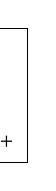
\begin{tikzpicture}[trim axis left, trim axis right]

\begin{axis}[%
width=\figurewidth,
height=\figureheight,
at={(0\figurewidth,0\figureheight)},
scale only axis,
every outer x axis line/.append style={black},
every x tick label/.append style={font=\color{black}},
xmin=9.5,
xmax=16,
xlabel={Time (h)},
every outer y axis line/.append style={black},
every y tick label/.append style={font=\color{black}},
ymin=-0.5,
ymax=0.5,
ylabel={Normalized Book Value},
axis background/.style={fill=white},
axis x line*=bottom,
axis y line*=left,
legend style={legend cell align=left,align=left,draw=black,font=\footnotesize, at={(0.98,0.02)},anchor=south east}
]
\addplot [color=black,solid]
  table[row sep=crcr]{%
9.50027777777778	0\\
9.50583333333333	9.81519360763183e-05\\
9.51138888888889	0.000227034157344486\\
9.51694444444444	0.000308206079452145\\
9.5225	0.000258924321714149\\
9.52805555555556	0.000280913359705037\\
9.53361111111111	0.000279411002689134\\
9.53916666666667	0.00032437302890842\\
9.54472222222222	0.000426180282143918\\
9.55027777777778	0.00045047657628694\\
9.55583333333333	0.000481933344987473\\
9.56138888888889	0.000495138309092091\\
9.56694444444444	0.000564246454493489\\
9.5725	0.000635676628396142\\
9.57805555555555	0.000641249740960026\\
9.58361111111111	0.000654071008446611\\
9.58916666666667	0.00067737672024637\\
9.59472222222222	0.000693045469473796\\
9.60027777777778	0.000695757941136632\\
9.60583333333333	0.000735818587615622\\
9.61138888888889	0.00075825814704622\\
9.61694444444444	0.000761800092015763\\
9.6225	0.000778494426121323\\
9.62805555555556	0.000807835182585981\\
9.63361111111111	0.00077699889261762\\
9.63916666666667	0.000823551945501544\\
9.64472222222222	0.00091284250505641\\
9.65027777777778	0.000873685271362445\\
9.65583333333333	0.000814049896137758\\
9.66138888888889	0.000791292796282761\\
9.66694444444444	0.000747372236710175\\
9.6725	0.000815751213834259\\
9.67805555555555	0.000808195071659856\\
9.68361111111111	0.000816735833472526\\
9.68916666666667	0.000850915718536127\\
9.69472222222222	0.000946265734872442\\
9.70027777777778	0.000953999149510887\\
9.70583333333333	0.000929395229309238\\
9.71138888888889	0.00093979415586265\\
9.71694444444444	0.00092454341972803\\
9.7225	0.000956937433033378\\
9.72805555555555	0.000999761139939714\\
9.73361111111111	0.00103887226853261\\
9.73916666666667	0.00100190680078649\\
9.74472222222222	0.00104725816723117\\
9.75027777777778	0.00102153442572939\\
9.75583333333333	0.00102692929924664\\
9.76138888888889	0.00103682241481406\\
9.76694444444444	0.00103266835348514\\
9.7725	0.00105151631710587\\
9.77805555555556	0.00104272164584795\\
9.78361111111111	0.00102230411732718\\
9.78916666666667	0.00104896994647308\\
9.79472222222222	0.00103918177071671\\
9.80027777777778	0.00105121005631093\\
9.80583333333333	0.00113043812378222\\
9.81138888888889	0.00116038716077926\\
9.81694444444444	0.00118617602384474\\
9.8225	0.00118507455133354\\
9.82805555555555	0.00122237784116552\\
9.83361111111111	0.00118207732208453\\
9.83916666666667	0.00120028501673675\\
9.84472222222222	0.00120072847718755\\
9.85027777777778	0.00117973599203447\\
9.85583333333333	0.00121740204842724\\
9.86138888888889	0.00117284627763681\\
9.86694444444444	0.00114937638829149\\
9.8725	0.00117308498445623\\
9.87805555555556	0.00120497432409827\\
9.88361111111111	0.00116935768673887\\
9.88916666666667	0.00119865509452421\\
9.89472222222222	0.00119056630708902\\
9.90027777777778	0.00116925717618122\\
9.90583333333333	0.00118743459984749\\
9.91138888888889	0.00123068284678673\\
9.91694444444444	0.00126676443209917\\
9.9225	0.00122949973817432\\
9.92805555555555	0.00123036213753935\\
9.93361111111111	0.00125360078662307\\
9.93916666666667	0.00124660143039335\\
9.94472222222222	0.00120856708942729\\
9.95027777777778	0.00125385404866574\\
9.95583333333333	0.00128328616189899\\
9.96138888888889	0.00127700907905037\\
9.96694444444444	0.00127146273108836\\
9.9725	0.00122787555924364\\
9.97805555555555	0.00119716032991746\\
9.98361111111111	0.0012179660110474\\
9.98916666666667	0.00117064396124955\\
9.99472222222222	0.00116155982670851\\
10.0002777777778	0.00124149953544372\\
10.0058333333333	0.00121528770872636\\
10.0113888888889	0.00119894890318872\\
10.0169444444444	0.0012218575650611\\
10.0225	0.00120180261562419\\
10.0280555555556	0.00120801072717325\\
10.0336111111111	0.00118737493770271\\
10.0391666666667	0.00127331789234741\\
10.0447222222222	0.00123922696444656\\
10.0502777777778	0.00123984241226971\\
10.0558333333333	0.00127367654181998\\
10.0613888888889	0.00124679669380434\\
10.0669444444444	0.00121441425221369\\
10.0725	0.0011592179755191\\
10.0780555555556	0.00117828853031954\\
10.0836111111111	0.00117314861829221\\
10.0891666666667	0.00117824917687015\\
10.0947222222222	0.00116969353823992\\
10.1002777777778	0.00114758137408977\\
10.1058333333333	0.00113772718010896\\
10.1113888888889	0.00114475574224149\\
10.1169444444444	0.00115145106271064\\
10.1225	0.00118170288765707\\
10.1280555555556	0.00119795997401528\\
10.1336111111111	0.00123809788073714\\
10.1391666666667	0.0012404875935772\\
10.1447222222222	0.00123752217604922\\
10.1502777777778	0.00121116519380227\\
10.1558333333333	0.00121434991253855\\
10.1613888888889	0.00124059439876567\\
10.1669444444444	0.00122089368964406\\
10.1725	0.00121132433049298\\
10.1780555555556	0.00125484704528822\\
10.1836111111111	0.00123739705741577\\
10.1891666666667	0.0012523548646528\\
10.1947222222222	0.00125335350532541\\
10.2002777777778	0.00126090463426554\\
10.2058333333333	0.00124983302784631\\
10.2113888888889	0.00123779289317105\\
10.2169444444444	0.00128319884118766\\
10.2225	0.00124498990298005\\
10.2280555555556	0.00120453161365841\\
10.2336111111111	0.00119148590723617\\
10.2391666666667	0.00120937259346943\\
10.2447222222222	0.00119257987593202\\
10.2502777777778	0.0012187594868549\\
10.2558333333333	0.00122364215902215\\
10.2613888888889	0.00122325678547153\\
10.2669444444444	0.00119366749660332\\
10.2725	0.00118947809466796\\
10.2780555555556	0.00120946942227862\\
10.2836111111111	0.00119909571445875\\
10.2891666666667	0.00121595361159232\\
10.2947222222222	0.00121282453875593\\
10.3002777777778	0.00121525321994143\\
10.3058333333333	0.00123775610393428\\
10.3113888888889	0.00124935094875767\\
10.3169444444444	0.00127320637377681\\
10.3225	0.0012916066203319\\
10.3280555555556	0.00130602337741959\\
10.3336111111111	0.00128922096455497\\
10.3391666666667	0.00131026393395928\\
10.3447222222222	0.00133239881538594\\
10.3502777777778	0.00132611199465815\\
10.3558333333333	0.00135719851957816\\
10.3613888888889	0.00134782121127253\\
10.3669444444444	0.00135335676428361\\
10.3725	0.00136251476936788\\
10.3780555555556	0.00138135814163864\\
10.3836111111111	0.00140043820009228\\
10.3891666666667	0.00139122131935232\\
10.3947222222222	0.00138194965898286\\
10.4002777777778	0.0014240425456733\\
10.4058333333333	0.00145274152308006\\
10.4113888888889	0.00140986681606092\\
10.4169444444444	0.00145157043820565\\
10.4225	0.00147377306481289\\
10.4280555555556	0.00144158456133225\\
10.4336111111111	0.00138801447985171\\
10.4391666666667	0.00142625727691215\\
10.4447222222222	0.00144102575131289\\
10.4502777777778	0.00146597876584709\\
10.4558333333333	0.00149173444746342\\
10.4613888888889	0.00150898485481088\\
10.4669444444444	0.00150003488282602\\
10.4725	0.00149922122630319\\
10.4780555555556	0.00151740015849722\\
10.4836111111111	0.00153140481828462\\
10.4891666666667	0.0015165822531451\\
10.4947222222222	0.00152967882793131\\
10.5002777777778	0.00149817348004389\\
10.5058333333333	0.00144976951066833\\
10.5113888888889	0.0014376187002485\\
10.5169444444444	0.00143743767446503\\
10.5225	0.00142500929764311\\
10.5280555555556	0.00142385885209562\\
10.5336111111111	0.00136706458531899\\
10.5391666666667	0.00136917897196343\\
10.5447222222222	0.00137193812665015\\
10.5502777777778	0.00138459036976313\\
10.5558333333333	0.00136969066496184\\
10.5613888888889	0.00134510176929692\\
10.5669444444444	0.00135695542834946\\
10.5725	0.00136279010015605\\
10.5780555555556	0.00139044420400802\\
10.5836111111111	0.00139871907772804\\
10.5891666666667	0.00137927354235612\\
10.5947222222222	0.0013970686486624\\
10.6002777777778	0.00136852263394616\\
10.6058333333333	0.00137394156903126\\
10.6113888888889	0.00137837900589921\\
10.6169444444444	0.00136790991917346\\
10.6225	0.00134927724106371\\
10.6280555555556	0.00132983724165436\\
10.6336111111111	0.0013048022508646\\
10.6391666666667	0.00132155271834744\\
10.6447222222222	0.00132501750605951\\
10.6502777777778	0.00130534843876418\\
10.6558333333333	0.00133352068806225\\
10.6613888888889	0.00131161029338722\\
10.6669444444444	0.00130898375945998\\
10.6725	0.00133609585437688\\
10.6780555555556	0.00134524646652801\\
10.6836111111111	0.00133822897290381\\
10.6891666666667	0.00135418649065344\\
10.6947222222222	0.00135785789076803\\
10.7002777777778	0.00133037341718434\\
10.7058333333333	0.00134416538054616\\
10.7113888888889	0.00133360071785904\\
10.7169444444444	0.00136151941971319\\
10.7225	0.00137649520987693\\
10.7280555555556	0.00137968204502292\\
10.7336111111111	0.00137743406162372\\
10.7391666666667	0.00143822478714695\\
10.7447222222222	0.00145460558837107\\
10.7502777777778	0.00143771788362135\\
10.7558333333333	0.00143048468140061\\
10.7613888888889	0.00141067979595855\\
10.7669444444444	0.00139090214405901\\
10.7725	0.00140009097728377\\
10.7780555555556	0.00140069605218085\\
10.7836111111111	0.00138199543680306\\
10.7891666666667	0.0013587123416765\\
10.7947222222222	0.00136568738130483\\
10.8002777777778	0.00135458621002837\\
10.8058333333333	0.0013568217828106\\
10.8113888888889	0.00132479221613657\\
10.8169444444444	0.00132933306010075\\
10.8225	0.00132554162740783\\
10.8280555555556	0.00130747622776073\\
10.8336111111111	0.00129032379411198\\
10.8391666666667	0.00128055263846671\\
10.8447222222222	0.00124695361801552\\
10.8502777777778	0.00125846240619931\\
10.8558333333333	0.00125419375300151\\
10.8613888888889	0.00121069256210005\\
10.8669444444444	0.00123551081282325\\
10.8725	0.00122938706332953\\
10.8780555555556	0.0012174850534814\\
10.8836111111111	0.00119959649751111\\
10.8891666666667	0.00123040406538433\\
10.8947222222222	0.0012137357508808\\
10.9002777777778	0.00120014142424174\\
10.9058333333333	0.00121417631545384\\
10.9113888888889	0.00119064598446994\\
10.9169444444444	0.00117219527458357\\
10.9225	0.00115849443157567\\
10.9280555555556	0.00111936896947706\\
10.9336111111111	0.00110913850949546\\
10.9391666666667	0.00112939419452784\\
10.9447222222222	0.0011243460451642\\
10.9502777777778	0.00113715277033544\\
10.9558333333333	0.00117429382798506\\
10.9613888888889	0.0011943982676188\\
10.9669444444444	0.00120119532070473\\
10.9725	0.00121223287411043\\
10.9780555555556	0.00120295531198589\\
10.9836111111111	0.00122149485477929\\
10.9891666666667	0.00120627514742266\\
10.9947222222222	0.00118706182198425\\
11.0002777777778	0.001141124847585\\
11.0058333333333	0.00112143190864256\\
11.0113888888889	0.00110768728088617\\
11.0169444444444	0.00109853667148574\\
11.0225	0.00107173568769126\\
11.0280555555556	0.00104674329952692\\
11.0336111111111	0.00102438802723692\\
11.0391666666667	0.00103392472693309\\
11.0447222222222	0.0010452424013061\\
11.0502777777778	0.00104041945056932\\
11.0558333333333	0.00106633515154275\\
11.0613888888889	0.00106534678243331\\
11.0669444444444	0.00106027162350886\\
11.0725	0.00107431928984059\\
11.0780555555556	0.00108324310625618\\
11.0836111111111	0.00108031346072912\\
11.0891666666667	0.00105325501580045\\
11.0947222222222	0.00102007715957164\\
11.1002777777778	0.00104337836525836\\
11.1058333333333	0.00104036554279618\\
11.1113888888889	0.00104918826749989\\
11.1169444444444	0.00107189120569617\\
11.1225	0.00111402340113131\\
11.1280555555556	0.00114408202821092\\
11.1336111111111	0.00112457131193189\\
11.1391666666667	0.00112779398838869\\
11.1447222222222	0.0010983423618931\\
11.1502777777778	0.00111736782797789\\
11.1558333333333	0.00111884827344477\\
11.1613888888889	0.00113239143498434\\
11.1669444444444	0.00113670133383326\\
11.1725	0.00116397067071672\\
11.1780555555556	0.00119907760926385\\
11.1836111111111	0.00120836052334972\\
11.1891666666667	0.00120388471393462\\
11.1947222222222	0.00122335340525015\\
11.2002777777778	0.00123351949191974\\
11.2058333333333	0.00124473943952008\\
11.2113888888889	0.00125157165972878\\
11.2169444444444	0.00127593777940493\\
11.2225	0.0012700371543215\\
11.2280555555556	0.00126636594121443\\
11.2336111111111	0.00125319621761411\\
11.2391666666667	0.00128812675681234\\
11.2447222222222	0.00129328169889886\\
11.2502777777778	0.00128184130221531\\
11.2558333333333	0.00132425893433274\\
11.2613888888889	0.00133097407511618\\
11.2669444444444	0.00133755278516801\\
11.2725	0.0013367204746717\\
11.2780555555556	0.00133027395142471\\
11.2836111111111	0.0013240517738351\\
11.2891666666667	0.00131225394183065\\
11.2947222222222	0.0013062976573015\\
11.3002777777778	0.00133807128613683\\
11.3058333333333	0.00134693783583861\\
11.3113888888889	0.001337542416884\\
11.3169444444444	0.00132004985062339\\
11.3225	0.00131373271898871\\
11.3280555555556	0.00131967702974434\\
11.3336111111111	0.00130661438160562\\
11.3391666666667	0.00131933102325776\\
11.3447222222222	0.00132033951540578\\
11.3502777777778	0.00133495569852671\\
11.3558333333333	0.00135470831584827\\
11.3613888888889	0.00136975784926774\\
11.3669444444444	0.00137556934945215\\
11.3725	0.00139404291548084\\
11.3780555555556	0.00136238215332174\\
11.3836111111111	0.00135748940610059\\
11.3891666666667	0.00133638455363605\\
11.3947222222222	0.00131350712645384\\
11.4002777777778	0.00130597111295527\\
11.4058333333333	0.00129185779716301\\
11.4113888888889	0.0013160766768423\\
11.4169444444444	0.00131670265987371\\
11.4225	0.00131714163184937\\
11.4280555555556	0.0013006126511772\\
11.4336111111111	0.00129762059091476\\
11.4391666666667	0.00131990055063458\\
11.4447222222222	0.00130364904183833\\
11.4502777777778	0.00129941242392184\\
11.4558333333333	0.00128666794203691\\
11.4613888888889	0.00131550712965245\\
11.4669444444444	0.00133778771054915\\
11.4725	0.00136776767910485\\
11.4780555555556	0.00138435901393819\\
11.4836111111111	0.00134467228864144\\
11.4891666666667	0.00132326974702068\\
11.4947222222222	0.00129736954930504\\
11.5002777777778	0.00128989501627164\\
11.5058333333333	0.0013301017723728\\
11.5113888888889	0.00132202885595079\\
11.5169444444444	0.00129893199697739\\
11.5225	0.0012899031255309\\
11.5280555555556	0.00129687820805069\\
11.5336111111111	0.001314975045688\\
11.5391666666667	0.00133928961510765\\
11.5447222222222	0.00131996286419422\\
11.5502777777778	0.00132543654703343\\
11.5558333333333	0.00136014134128049\\
11.5613888888889	0.00136343489014301\\
11.5669444444444	0.00135721991842619\\
11.5725	0.00139868407991561\\
11.5780555555556	0.00137406905250281\\
11.5836111111111	0.00138913175737265\\
11.5891666666667	0.00138361341033799\\
11.5947222222222	0.00138700026457728\\
11.6002777777778	0.00137019236048208\\
11.6058333333333	0.00136874144017174\\
11.6113888888889	0.00138230465565758\\
11.6169444444444	0.00138311329768959\\
11.6225	0.00136101867782612\\
11.6280555555556	0.00136797021753909\\
11.6336111111111	0.00135332347807404\\
11.6391666666667	0.00133523612176245\\
11.6447222222222	0.00133010409331469\\
11.6502777777778	0.00135848424048279\\
11.6558333333333	0.0013820316987605\\
11.6613888888889	0.00138767569807796\\
11.6669444444444	0.00139912230897221\\
11.6725	0.00139064846077219\\
11.6780555555556	0.00138618281229386\\
11.6836111111111	0.00142632236207274\\
11.6891666666667	0.00142387962603552\\
11.6947222222222	0.00143421071569194\\
11.7002777777778	0.00145876244497867\\
11.7058333333333	0.00144635623926681\\
11.7113888888889	0.00144163435246569\\
11.7169444444444	0.00144132143515385\\
11.7225	0.0014396961565637\\
11.7280555555556	0.00143339003905507\\
11.7336111111111	0.00141335068067971\\
11.7391666666667	0.00143325136770267\\
11.7447222222222	0.00144449333577934\\
11.7502777777778	0.00142752504443444\\
11.7558333333333	0.00145279319260005\\
11.7613888888889	0.00144819596101864\\
11.7669444444444	0.00145661954058052\\
11.7725	0.00145108346728628\\
11.7780555555556	0.00146286125719697\\
11.7836111111111	0.00144385213280329\\
11.7891666666667	0.00145366033027594\\
11.7947222222222	0.00144609856846101\\
11.8002777777778	0.00144114924685335\\
11.8058333333333	0.0014436665856763\\
11.8113888888889	0.00144267229409079\\
11.8169444444444	0.00141621242248569\\
11.8225	0.00141676254532941\\
11.8280555555556	0.00141949653492013\\
11.8336111111111	0.0014385868668001\\
11.8391666666667	0.00145820962499976\\
11.8447222222222	0.00145398998687751\\
11.8502777777778	0.0014572764551708\\
11.8558333333333	0.00144885192943023\\
11.8613888888889	0.00142343991319671\\
11.8669444444444	0.00140839314915175\\
11.8725	0.00141577945261639\\
11.8780555555556	0.0013927342472615\\
11.8836111111111	0.00135943560227392\\
11.8891666666667	0.00139811531957412\\
11.8947222222222	0.00139354960131799\\
11.9002777777778	0.00137765443939952\\
11.9058333333333	0.00138581797836856\\
11.9113888888889	0.00138310967939326\\
11.9169444444444	0.00139454761183933\\
11.9225	0.00141219062911135\\
11.9280555555556	0.00141686435851063\\
11.9336111111111	0.00140128085445856\\
11.9391666666667	0.00137967847013565\\
11.9447222222222	0.001379124663202\\
11.9502777777778	0.00135441052362784\\
11.9558333333333	0.00134467735971144\\
11.9613888888889	0.00133486244408521\\
11.9669444444444	0.00133091291585741\\
11.9725	0.0013293825997589\\
11.9780555555556	0.00134496734552503\\
11.9836111111111	0.00135397640904511\\
11.9891666666667	0.00137989318439113\\
11.9947222222222	0.00138835627771972\\
12.0002777777778	0.00141224790432481\\
12.0058333333333	0.00143207020234715\\
12.0113888888889	0.00144296442629233\\
12.0169444444444	0.00144828453793089\\
12.0225	0.00146234095705822\\
12.0280555555556	0.00146546620577892\\
12.0336111111111	0.00144092851751032\\
12.0391666666667	0.0014505163934504\\
12.0447222222222	0.00145099071776911\\
12.0502777777778	0.00144629478031599\\
12.0558333333333	0.00146177317026597\\
12.0613888888889	0.00145691903169909\\
12.0669444444444	0.00148749614905985\\
12.0725	0.00147177834351542\\
12.0780555555556	0.0014580185195292\\
12.0836111111111	0.00144882133570667\\
12.0891666666667	0.00146480645259395\\
12.0947222222222	0.00145280088025634\\
12.1002777777778	0.00144691962366061\\
12.1058333333333	0.00144458579499074\\
12.1113888888889	0.00144520929452829\\
12.1169444444444	0.00145286219357144\\
12.1225	0.00144863283596064\\
12.1280555555556	0.00145008106341393\\
12.1336111111111	0.00144291839507882\\
12.1391666666667	0.00143074400793908\\
12.1447222222222	0.00143407101986703\\
12.1502777777778	0.00143763350328685\\
12.1558333333333	0.00142162215373953\\
12.1613888888889	0.00143510430741856\\
12.1669444444444	0.00143037673484248\\
12.1725	0.00144076236977009\\
12.1780555555556	0.00146287765207043\\
12.1836111111111	0.00145222817480617\\
12.1891666666667	0.00147273837091322\\
12.1947222222222	0.00147369714346302\\
12.2002777777778	0.00147058653861754\\
12.2058333333333	0.0014622666672619\\
12.2113888888889	0.00146384230545893\\
12.2169444444444	0.00147942524499034\\
12.2225	0.00148665739321152\\
12.2280555555556	0.00149858509966339\\
12.2336111111111	0.00152743237339426\\
12.2391666666667	0.00156597688894533\\
12.2447222222222	0.00157147195193308\\
12.2502777777778	0.00158875292689276\\
12.2558333333333	0.00157491853167646\\
12.2613888888889	0.00156302493180149\\
12.2669444444444	0.0015678972078399\\
12.2725	0.00156946989553419\\
12.2780555555556	0.00156841739470925\\
12.2836111111111	0.00158760097609845\\
12.2891666666667	0.00158319269126195\\
12.2947222222222	0.00158851215414879\\
12.3002777777778	0.00160581399003012\\
12.3058333333333	0.00158613151907372\\
12.3113888888889	0.00162272728452639\\
12.3169444444444	0.00160635097779527\\
12.3225	0.0016024286844134\\
12.3280555555556	0.00159872670313876\\
12.3336111111111	0.00159159690225708\\
12.3391666666667	0.00158579529096237\\
12.3447222222222	0.00154547265125404\\
12.3502777777778	0.00154688506920775\\
12.3558333333333	0.00154138928145242\\
12.3613888888889	0.00152744504491387\\
12.3669444444444	0.00151977680176052\\
12.3725	0.00152541277200324\\
12.3780555555556	0.00151113145007375\\
12.3836111111111	0.00151154827873734\\
12.3891666666667	0.00149401332096755\\
12.3947222222222	0.00148879872206775\\
12.4002777777778	0.0014889467304986\\
12.4058333333333	0.00149070702887388\\
12.4113888888889	0.00147512692518337\\
12.4169444444444	0.00146557067474284\\
12.4225	0.00145597705749356\\
12.4280555555556	0.00145305608888435\\
12.4336111111111	0.00146234433280168\\
12.4391666666667	0.00142784691173681\\
12.4447222222222	0.00143511947290054\\
12.4502777777778	0.0014264462400877\\
12.4558333333333	0.00142608752868867\\
12.4613888888889	0.00141982536274776\\
12.4669444444444	0.00141603483412123\\
12.4725	0.00140129402473987\\
12.4780555555556	0.00139903098748539\\
12.4836111111111	0.00140989513755785\\
12.4891666666667	0.00140423438077009\\
12.4947222222222	0.00144134382270478\\
12.5002777777778	0.00142008324449527\\
12.5058333333333	0.00143049017881025\\
12.5113888888889	0.00142003730213625\\
12.5169444444444	0.00144325363107001\\
12.5225	0.00142994976944855\\
12.5280555555556	0.00140624224124153\\
12.5336111111111	0.00140785532246879\\
12.5391666666667	0.00140973841320102\\
12.5447222222222	0.00139854202024536\\
12.5502777777778	0.00142382540053299\\
12.5558333333333	0.00141985463132377\\
12.5613888888889	0.00143691498870546\\
12.5669444444444	0.00141589411350251\\
12.5725	0.00146187982744572\\
12.5780555555556	0.00146886736112473\\
12.5836111111111	0.00149180753452915\\
12.5891666666667	0.00149286771900314\\
12.5947222222222	0.00149719187465269\\
12.6002777777778	0.0014862965175888\\
12.6058333333333	0.00148741004871344\\
12.6113888888889	0.00149932692232468\\
12.6169444444444	0.00150074511144616\\
12.6225	0.00151112390409014\\
12.6280555555556	0.00150448392865843\\
12.6336111111111	0.00150657654265518\\
12.6391666666667	0.00151926194110752\\
12.6447222222222	0.00151568658776835\\
12.6502777777778	0.00150814711494873\\
12.6558333333333	0.00151566709108342\\
12.6613888888889	0.00149163061760316\\
12.6669444444444	0.00149900389316482\\
12.6725	0.0014942189245164\\
12.6780555555556	0.0014996395780269\\
12.6836111111111	0.00148760820917149\\
12.6891666666667	0.00149310204628916\\
12.6947222222222	0.0014788419267977\\
12.7002777777778	0.00146412621888659\\
12.7058333333333	0.00145275026913527\\
12.7113888888889	0.00146604937979555\\
12.7169444444444	0.00147986088096252\\
12.7225	0.00150730188134607\\
12.7280555555556	0.00149577419035762\\
12.7336111111111	0.00149975958070514\\
12.7391666666667	0.00153102126043603\\
12.7447222222222	0.00153938955259192\\
12.7502777777778	0.00154599058387173\\
12.7558333333333	0.00154942956131277\\
12.7613888888889	0.0015511460054709\\
12.7669444444444	0.00155465621642703\\
12.7725	0.00155835092517709\\
12.7780555555556	0.00155299702636058\\
12.7836111111111	0.00154895891144102\\
12.7891666666667	0.00154563909061878\\
12.7947222222222	0.00154856736301401\\
12.8002777777778	0.00152142116935639\\
12.8058333333333	0.00152680454154064\\
12.8113888888889	0.00152829166563939\\
12.8169444444444	0.00152933179492831\\
12.8225	0.00150175613639614\\
12.8280555555556	0.00151786488316596\\
12.8336111111111	0.00151893498870725\\
12.8391666666667	0.00152847714442328\\
12.8447222222222	0.00153352588890021\\
12.8502777777778	0.00151231860386303\\
12.8558333333333	0.0015073155021228\\
12.8613888888889	0.00149076872356768\\
12.8669444444444	0.001482533459783\\
12.8725	0.00149256813801757\\
12.8780555555556	0.00148953418766085\\
12.8836111111111	0.00146978859545643\\
12.8891666666667	0.00146899384230292\\
12.8947222222222	0.00146868213465479\\
12.9002777777778	0.00147179837056455\\
12.9058333333333	0.00147187990336795\\
12.9113888888889	0.00146460572528229\\
12.9169444444444	0.00146115704877481\\
12.9225	0.00147094811940152\\
12.9280555555556	0.00148314493470036\\
12.9336111111111	0.00147104998500613\\
12.9391666666667	0.00146797946556942\\
12.9447222222222	0.00148333876521312\\
12.9502777777778	0.00149510282061183\\
12.9558333333333	0.00149711174315503\\
12.9613888888889	0.00149025452025198\\
12.9669444444444	0.00146473616939047\\
12.9725	0.0014905251438968\\
12.9780555555556	0.00150978115350253\\
12.9836111111111	0.00152529101613141\\
12.9891666666667	0.00153050345268801\\
12.9947222222222	0.001520590370788\\
13.0002777777778	0.00133820703063137\\
13.0058333333333	0.00135071200503201\\
13.0113888888889	0.00135564948880296\\
13.0169444444444	0.00137097290859578\\
13.0225	0.0013809258353159\\
13.0280555555556	0.00140225667406102\\
13.0336111111111	0.00141686002217378\\
13.0391666666667	0.00140540296141367\\
13.0447222222222	0.00140744821136929\\
13.0502777777778	0.00140084130416684\\
13.0558333333333	0.00140787147778099\\
13.0613888888889	0.00140496910749777\\
13.0669444444444	0.00141458156183516\\
13.0725	0.00143575888119196\\
13.0780555555556	0.00143313654068455\\
13.0836111111111	0.00144874327548594\\
13.0891666666667	0.00144099731728509\\
13.0947222222222	0.00144900706120943\\
13.1002777777778	0.00144471327241935\\
13.1058333333333	0.00145038670480235\\
13.1113888888889	0.0014712027004038\\
13.1169444444444	0.00146149121981698\\
13.1225	0.00146481097213957\\
13.1280555555556	0.00148012130379582\\
13.1336111111111	0.00148519063223906\\
13.1391666666667	0.00146445061203249\\
13.1447222222222	0.00143902985726063\\
13.1502777777778	0.00142615011797842\\
13.1558333333333	0.00143566889910041\\
13.1613888888889	0.00142444863383662\\
13.1669444444444	0.00140081958338034\\
13.1725	0.0014043095810905\\
13.1780555555556	0.00141927713830481\\
13.1836111111111	0.00142168431754586\\
13.1891666666667	0.00144290154449678\\
13.1947222222222	0.00141707861186968\\
13.2002777777778	0.0013930204280006\\
13.2058333333333	0.00141168837388972\\
13.2113888888889	0.00139501500807482\\
13.2169444444444	0.00138739272409882\\
13.2225	0.00139944197168962\\
13.2280555555556	0.00141395895007346\\
13.2336111111111	0.00142749633867401\\
13.2391666666667	0.00143118693390409\\
13.2447222222222	0.00141093659673031\\
13.2502777777778	0.00138640668204948\\
13.2558333333333	0.00138229725256456\\
13.2613888888889	0.00138958404443534\\
13.2669444444444	0.00138546892552105\\
13.2725	0.00135807333939564\\
13.2780555555556	0.00137563460604162\\
13.2836111111111	0.00137950475476356\\
13.2891666666667	0.00141424061347584\\
13.2947222222222	0.00142259502273046\\
13.3002777777778	0.00140593008157608\\
13.3058333333333	0.00142100330683337\\
13.3113888888889	0.00144541509415741\\
13.3169444444444	0.001453397552587\\
13.3225	0.00146518700598852\\
13.3280555555556	0.00145000143429641\\
13.3336111111111	0.00143898474245274\\
13.3391666666667	0.00144375555558995\\
13.3447222222222	0.00144392288545725\\
13.3502777777778	0.00145832046977246\\
13.3558333333333	0.00144858797030833\\
13.3613888888889	0.00141908365009957\\
13.3669444444444	0.00140334378080786\\
13.3725	0.00141550894860409\\
13.3780555555556	0.00142529960548088\\
13.3836111111111	0.00141968152420624\\
13.3891666666667	0.0014388940104566\\
13.3947222222222	0.00144592101743957\\
13.4002777777778	0.00145945811075809\\
13.4058333333333	0.00147583083301672\\
13.4113888888889	0.0014794052458369\\
13.4169444444444	0.00148636598090413\\
13.4225	0.00148532452148098\\
13.4280555555556	0.00147663440647161\\
13.4336111111111	0.00150329062032362\\
13.4391666666667	0.00150338604490519\\
13.4447222222222	0.00150221298196929\\
13.4502777777778	0.00150691772765565\\
13.4558333333333	0.00150760459360266\\
13.4613888888889	0.00151288971893249\\
13.4669444444444	0.00150447215272242\\
13.4725	0.00150657566688861\\
13.4780555555556	0.00153773626914755\\
13.4836111111111	0.00153643528083025\\
13.4891666666667	0.00152058436723035\\
13.4947222222222	0.00150950563149643\\
13.5002777777778	0.00151462218849763\\
13.5058333333333	0.00152626819082768\\
13.5113888888889	0.00150467178989189\\
13.5169444444444	0.0014969634855273\\
13.5225	0.00148871293941832\\
13.5280555555556	0.00148314491468704\\
13.5336111111111	0.00148843240032726\\
13.5391666666667	0.00150295584220506\\
13.5447222222222	0.00149437573135303\\
13.5502777777778	0.00148678632958799\\
13.5558333333333	0.00147543500006719\\
13.5613888888889	0.00148878196322877\\
13.5669444444444	0.00148251988110615\\
13.5725	0.0014910363316345\\
13.5780555555556	0.00150492405516323\\
13.5836111111111	0.0014993878934948\\
13.5891666666667	0.00150318671892125\\
13.5947222222222	0.00150335210952468\\
13.6002777777778	0.00151897140934176\\
13.6058333333333	0.0015275195889668\\
13.6113888888889	0.00154351842196387\\
13.6169444444444	0.00153396159622998\\
13.6225	0.00152277395301437\\
13.6280555555556	0.00153783797758078\\
13.6336111111111	0.00149452044471743\\
13.6391666666667	0.00149843852998055\\
13.6447222222222	0.00149749949375511\\
13.6502777777778	0.00149044501928253\\
13.6558333333333	0.00149557190554694\\
13.6613888888889	0.00147004635112857\\
13.6669444444444	0.00147348258649505\\
13.6725	0.00149187643107962\\
13.6780555555556	0.00147382336950508\\
13.6836111111111	0.00146898762503\\
13.6891666666667	0.00146231941731756\\
13.6947222222222	0.00146131505750646\\
13.7002777777778	0.00143427218440095\\
13.7058333333333	0.00143367334281042\\
13.7113888888889	0.00145052404654833\\
13.7169444444444	0.00146356581079021\\
13.7225	0.00145908141962248\\
13.7280555555556	0.00147648883575746\\
13.7336111111111	0.00146964612855105\\
13.7391666666667	0.00147781508652733\\
13.7447222222222	0.00147924596833859\\
13.7502777777778	0.0014857211802215\\
13.7558333333333	0.00149796310375239\\
13.7613888888889	0.00149770707076158\\
13.7669444444444	0.0015057944750605\\
13.7725	0.00149311388196982\\
13.7780555555556	0.00149221180949777\\
13.7836111111111	0.00150406706345074\\
13.7891666666667	0.00153108224602549\\
13.7947222222222	0.00153690267945517\\
13.8002777777778	0.00153649447025694\\
13.8058333333333	0.00151269628342998\\
13.8113888888889	0.00152544777673813\\
13.8169444444444	0.00152753668026229\\
13.8225	0.00150735297540239\\
13.8280555555556	0.00147645117533535\\
13.8336111111111	0.00147955915642806\\
13.8391666666667	0.00147846096331428\\
13.8447222222222	0.00149402560538414\\
13.8502777777778	0.00147164251631104\\
13.8558333333333	0.0014729882999418\\
13.8613888888889	0.00146050151471311\\
13.8669444444444	0.00146028051542668\\
13.8725	0.0014355157843835\\
13.8780555555556	0.00146772345423285\\
13.8836111111111	0.00146731963961577\\
13.8891666666667	0.00146426562082946\\
13.8947222222222	0.00146675529036844\\
13.9002777777778	0.00146507352732739\\
13.9058333333333	0.00146260509071361\\
13.9113888888889	0.00144342510213558\\
13.9169444444444	0.00144697627366042\\
13.9225	0.00145155589475632\\
13.9280555555556	0.00145110220392852\\
13.9336111111111	0.00144888307947078\\
13.9391666666667	0.00143093618472623\\
13.9447222222222	0.00140834331000739\\
13.9502777777778	0.00140967069536413\\
13.9558333333333	0.00142490296180076\\
13.9613888888889	0.00142888837114774\\
13.9669444444444	0.0014053227869284\\
13.9725	0.00141081165286194\\
13.9780555555556	0.00135795173580666\\
13.9836111111111	0.00136031936557668\\
13.9891666666667	0.00136747822064986\\
13.9947222222222	0.00136561592603224\\
14.0002777777778	0.00137928129093678\\
14.0058333333333	0.00137974220761983\\
14.0113888888889	0.00136765221452384\\
14.0169444444444	0.00135790451754403\\
14.0225	0.00133242018945845\\
14.0280555555556	0.00132917226024176\\
14.0336111111111	0.00134689758229301\\
14.0391666666667	0.00136327304169437\\
14.0447222222222	0.00135647547208562\\
14.0502777777778	0.00136304720909219\\
14.0558333333333	0.00135620535922554\\
14.0613888888889	0.00135722705275332\\
14.0669444444444	0.00134741608470712\\
14.0725	0.00134420417788994\\
14.0780555555556	0.00134672860019958\\
14.0836111111111	0.001380317961722\\
14.0891666666667	0.00135617499927232\\
14.0947222222222	0.00136192405894953\\
14.1002777777778	0.00134772856460619\\
14.1058333333333	0.00134232266894863\\
14.1113888888889	0.00135362157389451\\
14.1169444444444	0.00134874340221303\\
14.1225	0.00134926620310494\\
14.1280555555556	0.00135735075134114\\
14.1336111111111	0.00135017189645636\\
14.1391666666667	0.0013278687025029\\
14.1447222222222	0.00132814982279772\\
14.1502777777778	0.00134163839263612\\
14.1558333333333	0.00132797235818849\\
14.1613888888889	0.00130375497950252\\
14.1669444444444	0.001307581340938\\
14.1725	0.00128351138783334\\
14.1780555555556	0.00127468268902087\\
14.1836111111111	0.00128628527918084\\
14.1891666666667	0.00126788050955806\\
14.1947222222222	0.00126288885137416\\
14.2002777777778	0.00125554940922834\\
14.2058333333333	0.0012599583444779\\
14.2113888888889	0.00124726168419897\\
14.2169444444444	0.00124482487614208\\
14.2225	0.00123626955873912\\
14.2280555555556	0.00120710287317993\\
14.2336111111111	0.00124440999907405\\
14.2391666666667	0.00124082314309826\\
14.2447222222222	0.00125241282302424\\
14.2502777777778	0.0012495993677506\\
14.2558333333333	0.00125803323465901\\
14.2613888888889	0.00126131937483809\\
14.2669444444444	0.0012360246569223\\
14.2725	0.0012541891200557\\
14.2780555555556	0.0012591921543319\\
14.2836111111111	0.00125570304372946\\
14.2891666666667	0.00125633024888305\\
14.2947222222222	0.00127182052213426\\
14.3002777777778	0.00126626525049711\\
14.3058333333333	0.00126826476175013\\
14.3113888888889	0.00126994667086788\\
14.3169444444444	0.00125842720299851\\
14.3225	0.00126585121477296\\
14.3280555555556	0.00127263712372638\\
14.3336111111111	0.00125927067645359\\
14.3391666666667	0.00127062773970721\\
14.3447222222222	0.00125564563851843\\
14.3502777777778	0.00127559362660046\\
14.3558333333333	0.00126873287997409\\
14.3613888888889	0.00126450172176784\\
14.3669444444444	0.00126435696943683\\
14.3725	0.00124198511449447\\
14.3780555555556	0.00123339311527038\\
14.3836111111111	0.00124394032144748\\
14.3891666666667	0.00126731949702452\\
14.3947222222222	0.00126739426399713\\
14.4002777777778	0.00127819784626815\\
14.4058333333333	0.00126890793866408\\
14.4113888888889	0.00127681839843485\\
14.4169444444444	0.00127544156824655\\
14.4225	0.00128841145662029\\
14.4280555555556	0.00128163979434648\\
14.4336111111111	0.00128938091194164\\
14.4391666666667	0.00131020423677031\\
14.4447222222222	0.00131182201395053\\
14.4502777777778	0.00132227358236192\\
14.4558333333333	0.00132625873247183\\
14.4613888888889	0.00131982439764822\\
14.4669444444444	0.00131643730625064\\
14.4725	0.00131930476315634\\
14.4780555555556	0.00130470583199371\\
14.4836111111111	0.0012981427955665\\
14.4891666666667	0.00128615860814518\\
14.4947222222222	0.00129632221144349\\
14.5002777777778	0.00127949107252667\\
14.5058333333333	0.00129270339956178\\
14.5113888888889	0.00130055704971288\\
14.5169444444444	0.00129874964662702\\
14.5225	0.00131611709924528\\
14.5280555555556	0.00126892156513336\\
14.5336111111111	0.00124270746191968\\
14.5391666666667	0.00124792852057909\\
14.5447222222222	0.00124572911155618\\
14.5502777777778	0.00123037951489535\\
14.5558333333333	0.00122553892476174\\
14.5613888888889	0.00123729749726342\\
14.5669444444444	0.0012411753743089\\
14.5725	0.00123784799946769\\
14.5780555555556	0.00123302667724245\\
14.5836111111111	0.00120358576691593\\
14.5891666666667	0.00120496121187497\\
14.5947222222222	0.00120935052282189\\
14.6002777777778	0.00119252063132991\\
14.6058333333333	0.0011723546355995\\
14.6113888888889	0.00114462096809498\\
14.6169444444444	0.00114215021541897\\
14.6225	0.00114585486354524\\
14.6280555555556	0.00115240104334702\\
14.6336111111111	0.00114449859055599\\
14.6391666666667	0.0011386487043834\\
14.6447222222222	0.0011355942582425\\
14.6502777777778	0.00112977317805374\\
14.6558333333333	0.00114255448611456\\
14.6613888888889	0.00115050156157293\\
14.6669444444444	0.00116887783376596\\
14.6725	0.00115741291607652\\
14.6780555555556	0.00117562441418873\\
14.6836111111111	0.00117583141010891\\
14.6891666666667	0.00116710465121783\\
14.6947222222222	0.00116347310793197\\
14.7002777777778	0.00115311473595558\\
14.7058333333333	0.00117169747597967\\
14.7113888888889	0.00116826558236327\\
14.7169444444444	0.00117963157995571\\
14.7225	0.0012115119405447\\
14.7280555555556	0.00122757226935777\\
14.7336111111111	0.00123304618459819\\
14.7391666666667	0.00124856580086652\\
14.7447222222222	0.00125219160131063\\
14.7502777777778	0.0012797068468049\\
14.7558333333333	0.00131037249886679\\
14.7613888888889	0.00130810137932635\\
14.7669444444444	0.00130669346071577\\
14.7725	0.00128279851835589\\
14.7780555555556	0.00126708323354863\\
14.7836111111111	0.0012715421660987\\
14.7891666666667	0.00128460065210034\\
14.7947222222222	0.00129904206294817\\
14.8002777777778	0.00128535559443388\\
14.8058333333333	0.00130490995145149\\
14.8113888888889	0.00130770524736379\\
14.8169444444444	0.0012953612240989\\
14.8225	0.00129399294094723\\
14.8280555555556	0.00129636156839741\\
14.8336111111111	0.00130256419756458\\
14.8391666666667	0.00131154543908218\\
14.8447222222222	0.00131405655031824\\
14.8502777777778	0.00129517138381607\\
14.8558333333333	0.00130649597032995\\
14.8613888888889	0.00129307814383028\\
14.8669444444444	0.00127775698016697\\
14.8725	0.00128600542217683\\
14.8780555555556	0.001294683466182\\
14.8836111111111	0.00128305283834229\\
14.8891666666667	0.00127758825540636\\
14.8947222222222	0.00128107760030449\\
14.9002777777778	0.00128140281044797\\
14.9058333333333	0.00128041868418105\\
14.9113888888889	0.00126431813782846\\
14.9169444444444	0.00126711052071848\\
14.9225	0.00127137713183645\\
14.9280555555556	0.00124666769132054\\
14.9336111111111	0.00127925656274086\\
14.9391666666667	0.00128082178676281\\
14.9447222222222	0.00127680637556105\\
14.9502777777778	0.00129062903501187\\
14.9558333333333	0.00127963745818738\\
14.9613888888889	0.00128395728926245\\
14.9669444444444	0.0012833550604463\\
14.9725	0.00128442860185807\\
14.9780555555556	0.00127234568190926\\
14.9836111111111	0.00126798248569626\\
14.9891666666667	0.00126595041061739\\
14.9947222222222	0.00126709902772393\\
15.0002777777778	0.00127087087059308\\
15.0058333333333	0.00125633145002069\\
15.0113888888889	0.0012570470184865\\
15.0169444444444	0.00125670310923542\\
15.0225	0.00125392993027273\\
15.0280555555556	0.00127198119725525\\
15.0336111111111	0.00127760379275776\\
15.0391666666667	0.0012853956009351\\
15.0447222222222	0.00127426464942748\\
15.0502777777778	0.00127336757131591\\
15.0558333333333	0.00130157798340513\\
15.0613888888889	0.00129165247891128\\
15.0669444444444	0.00127115584088955\\
15.0725	0.00127928189318038\\
15.0780555555556	0.00128530485433265\\
15.0836111111111	0.00128212395074878\\
15.0891666666667	0.0012942596697556\\
15.0947222222222	0.00130666180905536\\
15.1002777777778	0.00129454406558716\\
15.1058333333333	0.00130801401918301\\
15.1113888888889	0.00129222764829828\\
15.1169444444444	0.00127502308473049\\
15.1225	0.00127929300994856\\
15.1280555555556	0.00127354935187651\\
15.1336111111111	0.00128517467305178\\
15.1391666666667	0.00129443997317513\\
15.1447222222222	0.00128508163030916\\
15.1502777777778	0.00127313993716638\\
15.1558333333333	0.00129890236358832\\
15.1613888888889	0.00130246870926798\\
15.1669444444444	0.00129962501572511\\
15.1725	0.00129418677314908\\
15.1780555555556	0.00129692526535696\\
15.1836111111111	0.00127754132622027\\
15.1891666666667	0.00131073747344779\\
15.1947222222222	0.00131549511791684\\
15.2002777777778	0.00130586030684099\\
15.2058333333333	0.00129068978039104\\
15.2113888888889	0.0012676565708678\\
15.2169444444444	0.00126789718627318\\
15.2225	0.00126039112595944\\
15.2280555555556	0.00125666675628966\\
15.2336111111111	0.00128162497275897\\
15.2391666666667	0.00129652277874381\\
15.2447222222222	0.00130000957080889\\
15.2502777777778	0.00128905569881033\\
15.2558333333333	0.0012859669987868\\
15.2613888888889	0.00128216042333484\\
15.2669444444444	0.00131248460581967\\
15.2725	0.00130308467867324\\
15.2780555555556	0.00133570899680491\\
15.2836111111111	0.00133758724898714\\
15.2891666666667	0.00133133822346854\\
15.2947222222222	0.00131542048136235\\
15.3002777777778	0.00130596516965054\\
15.3058333333333	0.00133184297570899\\
15.3113888888889	0.0013138937402799\\
15.3169444444444	0.00129419436612443\\
15.3225	0.00129568978514083\\
15.3280555555556	0.00128190574584863\\
15.3336111111111	0.00128318641516723\\
15.3391666666667	0.00126645539499659\\
15.3447222222222	0.00125304267595649\\
15.3502777777778	0.00125791341724302\\
15.3558333333333	0.00125658339899615\\
15.3613888888889	0.00124691565718971\\
15.3669444444444	0.00126870497583886\\
15.3725	0.00127401176715636\\
15.3780555555556	0.00128175119238416\\
15.3836111111111	0.00128753679693405\\
15.3891666666667	0.00128633328578087\\
15.3947222222222	0.00129112053259517\\
15.4002777777778	0.00129366067519121\\
15.4058333333333	0.00126537115700764\\
15.4113888888889	0.00123013015160045\\
15.4169444444444	0.00122626211398158\\
15.4225	0.00123236758084988\\
15.4280555555556	0.00124107906030502\\
15.4336111111111	0.0012486251131103\\
15.4391666666667	0.00123752308489489\\
15.4447222222222	0.00121121763103815\\
15.4502777777778	0.00121738379529024\\
15.4558333333333	0.0012138698157913\\
15.4613888888889	0.00118931443769599\\
15.4669444444444	0.00122363976748896\\
15.4725	0.00121565634522791\\
15.4780555555556	0.0011979168863212\\
15.4836111111111	0.00118874126431923\\
15.4891666666667	0.00121690215716508\\
15.4947222222222	0.00123011071585277\\
15.5002777777778	0.00122800471722262\\
15.5058333333333	0.0012281601214863\\
15.5113888888889	0.00120974355084136\\
15.5169444444444	0.00119554733352079\\
15.5225	0.00121348331217552\\
15.5280555555556	0.00121401481616368\\
15.5336111111111	0.0012074352438558\\
15.5391666666667	0.00120813266800091\\
15.5447222222222	0.00118751831912123\\
15.5502777777778	0.00120289391104733\\
15.5558333333333	0.00117198199586843\\
15.5613888888889	0.00116127068120919\\
15.5669444444444	0.00114534278647715\\
15.5725	0.00115053016722566\\
15.5780555555556	0.00117229090087956\\
15.5836111111111	0.00117677245150793\\
15.5891666666667	0.00118999741995363\\
15.5947222222222	0.00119033622413167\\
15.6002777777778	0.00122243091527885\\
15.6058333333333	0.0012061785990749\\
15.6113888888889	0.00120167126818416\\
15.6169444444444	0.00121682729636596\\
15.6225	0.00123558310740823\\
15.6280555555556	0.00123657788838472\\
15.6336111111111	0.0012708233389056\\
15.6391666666667	0.0012918018701924\\
15.6447222222222	0.00130193816611501\\
15.6502777777778	0.00129899107476539\\
15.6558333333333	0.00129417643900198\\
15.6613888888889	0.00128098160975232\\
15.6669444444444	0.00128523595184515\\
15.6725	0.00127789477112694\\
15.6780555555556	0.00127606523598156\\
15.6836111111111	0.00129305374997335\\
15.6891666666667	0.00128634542426065\\
15.6947222222222	0.00130230732972403\\
15.7002777777778	0.00129447336967736\\
15.7058333333333	0.00129018288146066\\
15.7113888888889	0.00130233741517594\\
15.7169444444444	0.00129799740371017\\
15.7225	0.00129574991502701\\
15.7280555555556	0.00131111739925216\\
15.7336111111111	0.00129655760611191\\
15.7391666666667	0.00130649463834076\\
15.7447222222222	0.00134487280678175\\
15.7502777777778	0.00128869899621065\\
15.7558333333333	0.00122940675439298\\
15.7613888888889	0.00121979554366747\\
15.7669444444444	0.00121180257407905\\
15.7725	0.00115352370773758\\
15.7780555555556	0.00115106862597014\\
15.7836111111111	0.00111664091879482\\
15.7891666666667	0.00112294612202501\\
15.7947222222222	0.00110682458704892\\
15.8002777777778	0.00109488728901619\\
15.8058333333333	0.00108280686797158\\
15.8113888888889	0.00107464097144772\\
15.8169444444444	0.00106875720879951\\
15.8225	0.00104662101282482\\
15.8280555555556	0.00103306848306151\\
15.8336111111111	0.00104098131467856\\
15.8391666666667	0.00101226300611668\\
15.8447222222222	0.0010062031194138\\
15.8502777777778	0.00102389410635451\\
15.8558333333333	0.000975256936773139\\
15.8613888888889	0.000940717324369622\\
15.8669444444444	0.000915847198732944\\
15.8725	0.000890553482471912\\
15.8780555555556	0.000873303455763086\\
15.8836111111111	0.000866818424737348\\
15.8891666666667	0.000854982364537848\\
15.8947222222222	0.000858335459250625\\
15.9002777777778	0.000831456826839716\\
15.9058333333333	0.000817796398006276\\
15.9113888888889	0.00081837939059648\\
15.9169444444444	0.000777973819554578\\
15.9225	0.000781523340718238\\
15.9280555555556	0.000805054070758926\\
15.9336111111111	0.000836075753353427\\
15.9391666666667	0.000828453620822289\\
15.9447222222222	0.000837358458274151\\
15.9502777777778	0.000845262131508484\\
15.9558333333333	0.000854308828519112\\
15.9613888888889	0.000861330096132429\\
15.9669444444444	0.000865637614879677\\
15.9725	0.000841866606388297\\
15.9780555555556	0.000867252438703447\\
15.9836111111111	0.000878588908797662\\
15.9891666666667	0.000913653859965446\\
15.9947222222222	0.000893809586003158\\
};
\addlegendentry{Mid};

\addplot [color=red,solid]
  table[row sep=crcr]{%
9.50027777777778	0\\
9.50583333333333	-0.00129831852443265\\
9.51138888888889	-0.00236226427300193\\
9.51694444444444	-0.00314549408275527\\
9.5225	-0.00438673746812449\\
9.52805555555556	-0.00456019090647624\\
9.53361111111111	-0.00531473053356738\\
9.53916666666667	-0.0059322787237733\\
9.54472222222222	-0.0058341673717055\\
9.55027777777778	-0.00632905340082608\\
9.55583333333333	-0.00594051219714137\\
9.56138888888889	-0.00607931120641129\\
9.56694444444444	-0.00633993238899625\\
9.5725	-0.00649729800116604\\
9.57805555555555	-0.0066957576530861\\
9.58361111111111	-0.0071997387820526\\
9.58916666666667	-0.00757146047758921\\
9.59472222222222	-0.00746177489310022\\
9.60027777777778	-0.0072878942732999\\
9.60583333333333	-0.00770249077430951\\
9.61138888888889	-0.0074957076973504\\
9.61694444444444	-0.00718880356401036\\
9.6225	-0.0071003955914199\\
9.62805555555556	-0.00706932275625023\\
9.63361111111111	-0.00782522964291969\\
9.63916666666667	-0.00786239292880246\\
9.64472222222222	-0.00872976479884009\\
9.65027777777778	-0.00871519569834885\\
9.65583333333333	-0.00887157278517276\\
9.66138888888889	-0.00917946856637428\\
9.66694444444444	-0.00981381738721276\\
9.6725	-0.00955166271283391\\
9.67805555555555	-0.00982527606077179\\
9.68361111111111	-0.0101658947879507\\
9.68916666666667	-0.00934354720522032\\
9.69472222222222	-0.00960061740441546\\
9.70027777777778	-0.00880728906898987\\
9.70583333333333	-0.00864986616166217\\
9.71138888888889	-0.00918951983367369\\
9.71694444444444	-0.0100210646622255\\
9.7225	-0.010121179501293\\
9.72805555555555	-0.0106699622711067\\
9.73361111111111	-0.0109986733208075\\
9.73916666666667	-0.0113239792031975\\
9.74472222222222	-0.0106410012889047\\
9.75027777777778	-0.011995282539939\\
9.75583333333333	-0.0124906020576854\\
9.76138888888889	-0.0128597356307849\\
9.76694444444444	-0.0137223524086694\\
9.7725	-0.0143308128842188\\
9.77805555555556	-0.0138457826645069\\
9.78361111111111	-0.0143423180789892\\
9.78916666666667	-0.0144096391802556\\
9.79472222222222	-0.0142104386631551\\
9.80027777777778	-0.0134254866063196\\
9.80583333333333	-0.0131767008172377\\
9.81138888888889	-0.0134967285481535\\
9.81694444444444	-0.0127546763687914\\
9.8225	-0.0134025682361494\\
9.82805555555555	-0.0132279389230002\\
9.83361111111111	-0.0136922772551383\\
9.83916666666667	-0.0140167309016062\\
9.84472222222222	-0.0144012673594294\\
9.85027777777778	-0.0142957591692372\\
9.85583333333333	-0.0143157214548631\\
9.86138888888889	-0.0156811864991269\\
9.86694444444444	-0.0151214659974633\\
9.8725	-0.0147753477037211\\
9.87805555555556	-0.0152635623337301\\
9.88361111111111	-0.0153934463074421\\
9.88916666666667	-0.0153779480520008\\
9.89472222222222	-0.0159137021046068\\
9.90027777777778	-0.0163063779336562\\
9.90583333333333	-0.0160870207492175\\
9.91138888888889	-0.0154410169970615\\
9.91694444444444	-0.0154860023471257\\
9.9225	-0.0160142057094632\\
9.92805555555555	-0.0169252947449997\\
9.93361111111111	-0.0159988932732804\\
9.93916666666667	-0.0170080365572405\\
9.94472222222222	-0.0182905586569816\\
9.95027777777778	-0.0187291677772868\\
9.95583333333333	-0.0185572301235333\\
9.96138888888889	-0.0194012192557728\\
9.96694444444444	-0.0197361483215324\\
9.9725	-0.0197876128413591\\
9.97805555555555	-0.019754618032187\\
9.98361111111111	-0.0192671994884478\\
9.98916666666667	-0.0198700236055399\\
9.99472222222222	-0.0196270606765705\\
10.0002777777778	-0.0193874817348364\\
10.0058333333333	-0.0194215749917914\\
10.0113888888889	-0.0201397336290166\\
10.0169444444444	-0.0189165286578433\\
10.0225	-0.0189614051043042\\
10.0280555555556	-0.0192397313055872\\
10.0336111111111	-0.0195733440982948\\
10.0391666666667	-0.0189692107036994\\
10.0447222222222	-0.0185230215022467\\
10.0502777777778	-0.0181049432669279\\
10.0558333333333	-0.0181399165932164\\
10.0613888888889	-0.0185424963349725\\
10.0669444444444	-0.0189070880081399\\
10.0725	-0.0186443745685168\\
10.0780555555556	-0.01837704801055\\
10.0836111111111	-0.0196099341087996\\
10.0891666666667	-0.0202956598365806\\
10.0947222222222	-0.0206749071384303\\
10.1002777777778	-0.0215058550011543\\
10.1058333333333	-0.0211006864707938\\
10.1113888888889	-0.0214853182337264\\
10.1169444444444	-0.0216300086737956\\
10.1225	-0.0218171399165637\\
10.1280555555556	-0.0223759416082117\\
10.1336111111111	-0.0227578519002059\\
10.1391666666667	-0.022407727886577\\
10.1447222222222	-0.0236712731713734\\
10.1502777777778	-0.0223465660072429\\
10.1558333333333	-0.0228177881238363\\
10.1613888888889	-0.0237143649123311\\
10.1669444444444	-0.0236546198703317\\
10.1725	-0.0234555164104502\\
10.1780555555556	-0.0229367156505097\\
10.1836111111111	-0.0235998123561923\\
10.1891666666667	-0.0234545888848408\\
10.1947222222222	-0.0247019978659988\\
10.2002777777778	-0.02323602381049\\
10.2058333333333	-0.0236262296388499\\
10.2113888888889	-0.0236735026323036\\
10.2169444444444	-0.0233736622114824\\
10.2225	-0.0234087054745292\\
10.2280555555556	-0.024398634228093\\
10.2336111111111	-0.0242543963916167\\
10.2391666666667	-0.0240434459163088\\
10.2447222222222	-0.0230356562833924\\
10.2502777777778	-0.0221022569556487\\
10.2558333333333	-0.0227164026964081\\
10.2613888888889	-0.0228556944509889\\
10.2669444444444	-0.0238565272634128\\
10.2725	-0.023244688859305\\
10.2780555555556	-0.0220937599154218\\
10.2836111111111	-0.022282020468443\\
10.2891666666667	-0.0218831145702796\\
10.2947222222222	-0.0224034069229473\\
10.3002777777778	-0.0224540941080495\\
10.3058333333333	-0.022594069885925\\
10.3113888888889	-0.0214248723384326\\
10.3169444444444	-0.0216116004029343\\
10.3225	-0.0214082898296583\\
10.3280555555556	-0.0221556286861234\\
10.3336111111111	-0.0227084058582444\\
10.3391666666667	-0.022855327330622\\
10.3447222222222	-0.0228856553622438\\
10.3502777777778	-0.0230670676522167\\
10.3558333333333	-0.0233340530311964\\
10.3613888888889	-0.0227197735608696\\
10.3669444444444	-0.0231368703735741\\
10.3725	-0.0236499585082084\\
10.3780555555556	-0.0244784254391543\\
10.3836111111111	-0.0251231267621329\\
10.3891666666667	-0.0255195488036291\\
10.3947222222222	-0.0256258865209043\\
10.4002777777778	-0.0246468736249473\\
10.4058333333333	-0.0246256661105083\\
10.4113888888889	-0.0254360528005398\\
10.4169444444444	-0.024847069438226\\
10.4225	-0.0244535472203982\\
10.4280555555556	-0.0239434057596492\\
10.4336111111111	-0.0244612597182157\\
10.4391666666667	-0.023204277424231\\
10.4447222222222	-0.0236106235723478\\
10.4502777777778	-0.0228837335070866\\
10.4558333333333	-0.0231960648533797\\
10.4613888888889	-0.0229660459982805\\
10.4669444444444	-0.0231298928451366\\
10.4725	-0.023362824037945\\
10.4780555555556	-0.0236296307618189\\
10.4836111111111	-0.0233025694709684\\
10.4891666666667	-0.0233818088765112\\
10.4947222222222	-0.0239543320368119\\
10.5002777777778	-0.0236239296506664\\
10.5058333333333	-0.025167177644812\\
10.5113888888889	-0.0248712773802932\\
10.5169444444444	-0.0250223557492309\\
10.5225	-0.0243733568185743\\
10.5280555555556	-0.0250019863110568\\
10.5336111111111	-0.0249716777060376\\
10.5391666666667	-0.025762131812438\\
10.5447222222222	-0.0262571803220233\\
10.5502777777778	-0.0255901363303427\\
10.5558333333333	-0.0255395048477662\\
10.5613888888889	-0.0257513045549716\\
10.5669444444444	-0.0258623016836431\\
10.5725	-0.027125062197426\\
10.5780555555556	-0.0267325631911272\\
10.5836111111111	-0.0274246697114117\\
10.5891666666667	-0.0267198942888742\\
10.5947222222222	-0.0264658214604294\\
10.6002777777778	-0.026716913207017\\
10.6058333333333	-0.0278739850714028\\
10.6113888888889	-0.0270836306264891\\
10.6169444444444	-0.0270547896293303\\
10.6225	-0.0277112099842375\\
10.6280555555556	-0.0283141391125994\\
10.6336111111111	-0.029236478353509\\
10.6391666666667	-0.0290518819620499\\
10.6447222222222	-0.0292703550900435\\
10.6502777777778	-0.0290303404463177\\
10.6558333333333	-0.0295961905297271\\
10.6613888888889	-0.0302916747001937\\
10.6669444444444	-0.030221093391368\\
10.6725	-0.0293796727204913\\
10.6780555555556	-0.0296459071410717\\
10.6836111111111	-0.0292000000113828\\
10.6891666666667	-0.0297076630183346\\
10.6947222222222	-0.0306390139228106\\
10.7002777777778	-0.030584696678547\\
10.7058333333333	-0.0300842662150683\\
10.7113888888889	-0.0305697248679661\\
10.7169444444444	-0.0312018664310453\\
10.7225	-0.0312261146226096\\
10.7280555555556	-0.0308487687246788\\
10.7336111111111	-0.0306041345061017\\
10.7391666666667	-0.0305220313005007\\
10.7447222222222	-0.0307557732392704\\
10.7502777777778	-0.0312829704821967\\
10.7558333333333	-0.0313628771153709\\
10.7613888888889	-0.0313669186642559\\
10.7669444444444	-0.0317376231666885\\
10.7725	-0.030859372102654\\
10.7780555555556	-0.0310769662555897\\
10.7836111111111	-0.0306684789132884\\
10.7891666666667	-0.0310224360812739\\
10.7947222222222	-0.0306162006663795\\
10.8002777777778	-0.0303683171676568\\
10.8058333333333	-0.0300691181840928\\
10.8113888888889	-0.0301783529287385\\
10.8169444444444	-0.0301025234639695\\
10.8225	-0.0297091872163018\\
10.8280555555556	-0.0292258830307556\\
10.8336111111111	-0.0294854864823076\\
10.8391666666667	-0.0295305620757424\\
10.8447222222222	-0.0301902606634472\\
10.8502777777778	-0.030157398728316\\
10.8558333333333	-0.0307625434050406\\
10.8613888888889	-0.031289693972143\\
10.8669444444444	-0.0328394327085263\\
10.8725	-0.0321125995850691\\
10.8780555555556	-0.0321100443654019\\
10.8836111111111	-0.033037736855825\\
10.8891666666667	-0.0332256208953829\\
10.8947222222222	-0.0329266096907667\\
10.9002777777778	-0.0328880301843116\\
10.9058333333333	-0.0329202089725275\\
10.9113888888889	-0.0332760796590734\\
10.9169444444444	-0.032931112036956\\
10.9225	-0.0329704102297361\\
10.9280555555556	-0.0317969655752428\\
10.9336111111111	-0.0307937279879533\\
10.9391666666667	-0.0315870589901356\\
10.9447222222222	-0.0312572255934563\\
10.9502777777778	-0.0310855452422238\\
10.9558333333333	-0.0305492205868143\\
10.9613888888889	-0.0307596994416735\\
10.9669444444444	-0.0322019719162614\\
10.9725	-0.0319453504784279\\
10.9780555555556	-0.0325814576155815\\
10.9836111111111	-0.0328325879894059\\
10.9891666666667	-0.0330513413988442\\
10.9947222222222	-0.0330646203499955\\
11.0002777777778	-0.033464525551588\\
11.0058333333333	-0.0332888326164327\\
11.0113888888889	-0.0331602975869154\\
11.0169444444444	-0.033707618240439\\
11.0225	-0.033168409729375\\
11.0280555555556	-0.0324299342802395\\
11.0336111111111	-0.0334794665120309\\
11.0391666666667	-0.0340277862798684\\
11.0447222222222	-0.0349335138364283\\
11.0502777777778	-0.0355610641814268\\
11.0558333333333	-0.0360082060966366\\
11.0613888888889	-0.0365063620169075\\
11.0669444444444	-0.0367398635624335\\
11.0725	-0.0367396198035382\\
11.0780555555556	-0.0372847274073498\\
11.0836111111111	-0.0381566760358754\\
11.0891666666667	-0.0389242122007988\\
11.0947222222222	-0.0394164696912185\\
11.1002777777778	-0.0399523922496211\\
11.1058333333333	-0.0390779823563606\\
11.1113888888889	-0.0392027337987106\\
11.1169444444444	-0.0396701880755633\\
11.1225	-0.0386478741202012\\
11.1280555555556	-0.0367193827870001\\
11.1336111111111	-0.0379775288685036\\
11.1391666666667	-0.0386044828831651\\
11.1447222222222	-0.0383511582460127\\
11.1502777777778	-0.0383217949542396\\
11.1558333333333	-0.0378011049561748\\
11.1613888888889	-0.0388889744183184\\
11.1669444444444	-0.0381820601865794\\
11.1725	-0.0373200907454738\\
11.1780555555556	-0.0372183642266987\\
11.1836111111111	-0.0370252751167649\\
11.1891666666667	-0.03638753751485\\
11.1947222222222	-0.0359790150911772\\
11.2002777777778	-0.0364837356872898\\
11.2058333333333	-0.0358774073521907\\
11.2113888888889	-0.0357678165880501\\
11.2169444444444	-0.0358359426621147\\
11.2225	-0.0359534304884394\\
11.2280555555556	-0.0354152769703009\\
11.2336111111111	-0.0351652837954948\\
11.2391666666667	-0.0352569458376744\\
11.2447222222222	-0.0354539440122195\\
11.2502777777778	-0.0357537758212592\\
11.2558333333333	-0.0352171750922148\\
11.2613888888889	-0.0353340477296227\\
11.2669444444444	-0.0344060766176645\\
11.2725	-0.0348876768319312\\
11.2780555555556	-0.034814435056106\\
11.2836111111111	-0.0350763969544593\\
11.2891666666667	-0.0349459994918879\\
11.2947222222222	-0.0351072046176267\\
11.3002777777778	-0.0354986996299758\\
11.3058333333333	-0.0354413837474266\\
11.3113888888889	-0.0348598423777131\\
11.3169444444444	-0.0348095677203169\\
11.3225	-0.0343177158432238\\
11.3280555555556	-0.0343620281524956\\
11.3336111111111	-0.0351558044597663\\
11.3391666666667	-0.0347626057324717\\
11.3447222222222	-0.0340537568750017\\
11.3502777777778	-0.0350534567666977\\
11.3558333333333	-0.0349493634046671\\
11.3613888888889	-0.0356698739204686\\
11.3669444444444	-0.0360032819025423\\
11.3725	-0.0356394275264244\\
11.3780555555556	-0.036211704099937\\
11.3836111111111	-0.0361411103076126\\
11.3891666666667	-0.0366512702059502\\
11.3947222222222	-0.0364667616495061\\
11.4002777777778	-0.0359026937753212\\
11.4058333333333	-0.0354551263693993\\
11.4113888888889	-0.0354202355464216\\
11.4169444444444	-0.0358020806270496\\
11.4225	-0.0361415365224175\\
11.4280555555556	-0.0358816739683477\\
11.4336111111111	-0.0363496121363566\\
11.4391666666667	-0.0359829180371724\\
11.4447222222222	-0.0364382858120323\\
11.4502777777778	-0.036046878575359\\
11.4558333333333	-0.036161493438413\\
11.4613888888889	-0.0346855896565002\\
11.4669444444444	-0.0345660596508868\\
11.4725	-0.0349313109877361\\
11.4780555555556	-0.0351607417669123\\
11.4836111111111	-0.0345672760244684\\
11.4891666666667	-0.0358686158857472\\
11.4947222222222	-0.0354369340926252\\
11.5002777777778	-0.035894138194448\\
11.5058333333333	-0.0351688945555139\\
11.5113888888889	-0.0355824249705253\\
11.5169444444444	-0.0358423185642294\\
11.5225	-0.0350292001609789\\
11.5280555555556	-0.0349446462622665\\
11.5336111111111	-0.034657379104465\\
11.5391666666667	-0.0343827264740981\\
11.5447222222222	-0.0348077889084313\\
11.5502777777778	-0.0341410975023049\\
11.5558333333333	-0.034203128308942\\
11.5613888888889	-0.034659386108561\\
11.5669444444444	-0.0334369739921128\\
11.5725	-0.0343245271841685\\
11.5780555555556	-0.0341944666521245\\
11.5836111111111	-0.0344052298368449\\
11.5891666666667	-0.0354166723141631\\
11.5947222222222	-0.0354408069787062\\
11.6002777777778	-0.0363769848751995\\
11.6058333333333	-0.0367027714226378\\
11.6113888888889	-0.0366782757356492\\
11.6169444444444	-0.0356412753823913\\
11.6225	-0.036219148140654\\
11.6280555555556	-0.0364135142376226\\
11.6336111111111	-0.0367738085181046\\
11.6391666666667	-0.035802698211014\\
11.6447222222222	-0.0364251278142617\\
11.6502777777778	-0.0359377684932055\\
11.6558333333333	-0.0352050379533004\\
11.6613888888889	-0.0348306247583161\\
11.6669444444444	-0.0353017128138796\\
11.6725	-0.0352591433853078\\
11.6780555555556	-0.0361602054273223\\
11.6836111111111	-0.0357372869228936\\
11.6891666666667	-0.0351732101219715\\
11.6947222222222	-0.0352481092723833\\
11.7002777777778	-0.0348562557512667\\
11.7058333333333	-0.0351657077200314\\
11.7113888888889	-0.0346946380542449\\
11.7169444444444	-0.0342907674611864\\
11.7225	-0.0348766824367799\\
11.7280555555556	-0.0360764071788333\\
11.7336111111111	-0.0363910713405777\\
11.7391666666667	-0.0366520795879935\\
11.7447222222222	-0.0367169818205383\\
11.7502777777778	-0.0374608912460918\\
11.7558333333333	-0.0373400994140956\\
11.7613888888889	-0.0380433510969568\\
11.7669444444444	-0.0387810813523582\\
11.7725	-0.0391842085957748\\
11.7780555555556	-0.0390235279179838\\
11.7836111111111	-0.0393911391153128\\
11.7891666666667	-0.0397349193515061\\
11.7947222222222	-0.0396957081778995\\
11.8002777777778	-0.0400467657398823\\
11.8058333333333	-0.0402126536852278\\
11.8113888888889	-0.0403480813737098\\
11.8169444444444	-0.0397009581180711\\
11.8225	-0.0393513182441855\\
11.8280555555556	-0.0402368032624207\\
11.8336111111111	-0.0401828483284738\\
11.8391666666667	-0.0392760810564484\\
11.8447222222222	-0.0398562589225563\\
11.8502777777778	-0.0392745907476196\\
11.8558333333333	-0.0393502415699077\\
11.8613888888889	-0.0397489325997595\\
11.8669444444444	-0.0396678390556047\\
11.8725	-0.0409742794624356\\
11.8780555555556	-0.0408698369850972\\
11.8836111111111	-0.0415872665416562\\
11.8891666666667	-0.0400755974632517\\
11.8947222222222	-0.0394390928069258\\
11.9002777777778	-0.0397482333356252\\
11.9058333333333	-0.0398102518922548\\
11.9113888888889	-0.0399438156415541\\
11.9169444444444	-0.0396083155443352\\
11.9225	-0.0400752091470217\\
11.9280555555556	-0.0407553800303464\\
11.9336111111111	-0.0410494117289452\\
11.9391666666667	-0.0410247094237087\\
11.9447222222222	-0.0407195971566773\\
11.9502777777778	-0.0417551400357896\\
11.9558333333333	-0.041327253416509\\
11.9613888888889	-0.0404223202628782\\
11.9669444444444	-0.0399280624043098\\
11.9725	-0.0393940946911526\\
11.9780555555556	-0.0387860983094202\\
11.9836111111111	-0.038401334617717\\
11.9891666666667	-0.0389637305031723\\
11.9947222222222	-0.0390412019874956\\
12.0002777777778	-0.0396055677824492\\
12.0058333333333	-0.0398590553661111\\
12.0113888888889	-0.0403449333730657\\
12.0169444444444	-0.0407644605098032\\
12.0225	-0.0407268558295547\\
12.0280555555556	-0.0400619446408009\\
12.0336111111111	-0.0400643050995668\\
12.0391666666667	-0.0409902411857658\\
12.0447222222222	-0.0413091856382395\\
12.0502777777778	-0.0417591531645791\\
12.0558333333333	-0.0414344700956931\\
12.0613888888889	-0.0415985583499945\\
12.0669444444444	-0.0410457731865804\\
12.0725	-0.0407291313249318\\
12.0780555555556	-0.040538732895263\\
12.0836111111111	-0.0399452211417044\\
12.0891666666667	-0.0387650490741189\\
12.0947222222222	-0.039118116586792\\
12.1002777777778	-0.0399999464089434\\
12.1058333333333	-0.0402551361729176\\
12.1113888888889	-0.0413693855719013\\
12.1169444444444	-0.0416476675638783\\
12.1225	-0.0417613234018017\\
12.1280555555556	-0.0416187139834518\\
12.1336111111111	-0.042912895450938\\
12.1391666666667	-0.0429742674562028\\
12.1447222222222	-0.0437351956247384\\
12.1502777777778	-0.0441700853029481\\
12.1558333333333	-0.0447256728969787\\
12.1613888888889	-0.0451494429678133\\
12.1669444444444	-0.045338761944557\\
12.1725	-0.0445561687419999\\
12.1780555555556	-0.0441925874619138\\
12.1836111111111	-0.0439694025753526\\
12.1891666666667	-0.0433681064014628\\
12.1947222222222	-0.0427096883302354\\
12.2002777777778	-0.0433679747148496\\
12.2058333333333	-0.0439485106290218\\
12.2113888888889	-0.0436189530147331\\
12.2169444444444	-0.0428832748910439\\
12.2225	-0.0427763737132091\\
12.2280555555556	-0.0425489084957327\\
12.2336111111111	-0.0415823858031856\\
12.2391666666667	-0.0411920105055007\\
12.2447222222222	-0.0406028826749607\\
12.2502777777778	-0.0400487468743242\\
12.2558333333333	-0.0391885294245712\\
12.2613888888889	-0.0399795624547004\\
12.2669444444444	-0.0398807649693661\\
12.2725	-0.0409852967327945\\
12.2780555555556	-0.0414971229684922\\
12.2836111111111	-0.0407612307195967\\
12.2891666666667	-0.0411276527517845\\
12.2947222222222	-0.0407561924336925\\
12.3002777777778	-0.0397937597890274\\
12.3058333333333	-0.0399014723328778\\
12.3113888888889	-0.0389946849474342\\
12.3169444444444	-0.039463029172873\\
12.3225	-0.0391237759164113\\
12.3280555555556	-0.0405390762977382\\
12.3336111111111	-0.0402959303488848\\
12.3391666666667	-0.0413748889979979\\
12.3447222222222	-0.0420235178837625\\
12.3502777777778	-0.0422330019299215\\
12.3558333333333	-0.0422489977691752\\
12.3613888888889	-0.0420159993540728\\
12.3669444444444	-0.0418965759124106\\
12.3725	-0.0414513785966617\\
12.3780555555556	-0.0426038600908959\\
12.3836111111111	-0.0431079650490598\\
12.3891666666667	-0.0431053013652169\\
12.3947222222222	-0.0432852117589397\\
12.4002777777778	-0.043238042543791\\
12.4058333333333	-0.0426293399243065\\
12.4113888888889	-0.0428019152181069\\
12.4169444444444	-0.0434996922598715\\
12.4225	-0.0441137432976603\\
12.4280555555556	-0.0447550770405036\\
12.4336111111111	-0.0451703835129735\\
12.4391666666667	-0.0458405425837041\\
12.4447222222222	-0.0455630970886382\\
12.4502777777778	-0.0456160916094859\\
12.4558333333333	-0.046243216156107\\
12.4613888888889	-0.0463869250725063\\
12.4669444444444	-0.0467262007332754\\
12.4725	-0.0472067051353046\\
12.4780555555556	-0.0479096049729444\\
12.4836111111111	-0.0486847822291719\\
12.4891666666667	-0.0493094326612017\\
12.4947222222222	-0.0482972648098071\\
12.5002777777778	-0.0488487405563368\\
12.5058333333333	-0.0488050085024533\\
12.5113888888889	-0.0496191149097413\\
12.5169444444444	-0.0487884223982053\\
12.5225	-0.0488791969206591\\
12.5280555555556	-0.0493212403367779\\
12.5336111111111	-0.049128525722135\\
12.5391666666667	-0.0490445727760715\\
12.5447222222222	-0.0487839199715393\\
12.5502777777778	-0.0495603141490424\\
12.5558333333333	-0.0494667093570136\\
12.5613888888889	-0.0491746525612999\\
12.5669444444444	-0.0500472163061772\\
12.5725	-0.049858380442704\\
12.5780555555556	-0.0498191922743454\\
12.5836111111111	-0.0502240186693083\\
12.5891666666667	-0.0499706221701132\\
12.5947222222222	-0.0500420393873331\\
12.6002777777778	-0.0496768264149003\\
12.6058333333333	-0.0493788457089194\\
12.6113888888889	-0.0493704855633667\\
12.6169444444444	-0.0493954775104937\\
12.6225	-0.0492878740203562\\
12.6280555555556	-0.049912307269861\\
12.6336111111111	-0.0496081401120409\\
12.6391666666667	-0.0501403345649375\\
12.6447222222222	-0.0512995271711712\\
12.6502777777778	-0.0503417170399526\\
12.6558333333333	-0.0494024302122587\\
12.6613888888889	-0.0498136378849211\\
12.6669444444444	-0.0497816649673668\\
12.6725	-0.0500849087493031\\
12.6780555555556	-0.0506185865705751\\
12.6836111111111	-0.0520029639788629\\
12.6891666666667	-0.0522591047569248\\
12.6947222222222	-0.0524419557887286\\
12.7002777777778	-0.0521405706742747\\
12.7058333333333	-0.0531081043690625\\
12.7113888888889	-0.0525882686804605\\
12.7169444444444	-0.0536357974667679\\
12.7225	-0.0535564226593134\\
12.7280555555556	-0.0532549359954442\\
12.7336111111111	-0.0545945089338924\\
12.7391666666667	-0.0543279658009373\\
12.7447222222222	-0.055403113476271\\
12.7502777777778	-0.0544400806803985\\
12.7558333333333	-0.053609374069435\\
12.7613888888889	-0.0534100417218007\\
12.7669444444444	-0.0528327184289207\\
12.7725	-0.0533510309167342\\
12.7780555555556	-0.05406150544181\\
12.7836111111111	-0.0536548919127259\\
12.7891666666667	-0.0528422227169234\\
12.7947222222222	-0.0523976264835867\\
12.8002777777778	-0.0536143145265665\\
12.8058333333333	-0.0521386822154047\\
12.8113888888889	-0.0516839809507909\\
12.8169444444444	-0.0514560580651728\\
12.8225	-0.0510492835418746\\
12.8280555555556	-0.0516652182221722\\
12.8336111111111	-0.0512258679489196\\
12.8391666666667	-0.0507325655122269\\
12.8447222222222	-0.0509266117392791\\
12.8502777777778	-0.0510047206467282\\
12.8558333333333	-0.0506056662439851\\
12.8613888888889	-0.0509716752217479\\
12.8669444444444	-0.0504232350078116\\
12.8725	-0.0497530617991918\\
12.8780555555556	-0.0501284460699008\\
12.8836111111111	-0.0501833348997299\\
12.8891666666667	-0.0494487317780488\\
12.8947222222222	-0.0492279013354609\\
12.9002777777778	-0.0476014918875732\\
12.9058333333333	-0.0483571080294769\\
12.9113888888889	-0.0492106973313315\\
12.9169444444444	-0.0482818025154179\\
12.9225	-0.0491123265876595\\
12.9280555555556	-0.0497830150902832\\
12.9336111111111	-0.0500861184130208\\
12.9391666666667	-0.0505557020169181\\
12.9447222222222	-0.0500785676178222\\
12.9502777777778	-0.050034410704968\\
12.9558333333333	-0.0504389832724429\\
12.9613888888889	-0.0500183654062753\\
12.9669444444444	-0.0497748158661816\\
12.9725	-0.0497831300167357\\
12.9780555555556	-0.0493927852519322\\
12.9836111111111	-0.0488134267070476\\
12.9891666666667	-0.0484695667033044\\
12.9947222222222	-0.0487213447819069\\
13.0002777777778	-0.0494953930537801\\
13.0058333333333	-0.0497076380011122\\
13.0113888888889	-0.0495918416990783\\
13.0169444444444	-0.0506340892758771\\
13.0225	-0.0499102346724673\\
13.0280555555556	-0.0508316966163323\\
13.0336111111111	-0.0518878105505296\\
13.0391666666667	-0.0518744722490421\\
13.0447222222222	-0.0528123661240405\\
13.0502777777778	-0.0526459326938555\\
13.0558333333333	-0.05308625502518\\
13.0613888888889	-0.0526634242678276\\
13.0669444444444	-0.054140519036265\\
13.0725	-0.0547061661018413\\
13.0780555555556	-0.0539202856559896\\
13.0836111111111	-0.0531862623863451\\
13.0891666666667	-0.0527089049723119\\
13.0947222222222	-0.0532464949425463\\
13.1002777777778	-0.0527516992857732\\
13.1058333333333	-0.053587181555601\\
13.1113888888889	-0.0534340271698203\\
13.1169444444444	-0.0535780148079875\\
13.1225	-0.0539900442088368\\
13.1280555555556	-0.054366282472788\\
13.1336111111111	-0.053945733394596\\
13.1391666666667	-0.0543736918428719\\
13.1447222222222	-0.0539483268019772\\
13.1502777777778	-0.0546880384969979\\
13.1558333333333	-0.0535962373869453\\
13.1613888888889	-0.0543875043679095\\
13.1669444444444	-0.0529709023385162\\
13.1725	-0.053261807478537\\
13.1780555555556	-0.0519535256302417\\
13.1836111111111	-0.0528471737612425\\
13.1891666666667	-0.0539049443795869\\
13.1947222222222	-0.0534413674597852\\
13.2002777777778	-0.0531277531528237\\
13.2058333333333	-0.0541881668266024\\
13.2113888888889	-0.0533218415041119\\
13.2169444444444	-0.0536357456286761\\
13.2225	-0.0531087690835564\\
13.2280555555556	-0.0530600286707799\\
13.2336111111111	-0.0534790295868533\\
13.2391666666667	-0.0541011501527359\\
13.2447222222222	-0.0539308712129753\\
13.2502777777778	-0.0547112043820842\\
13.2558333333333	-0.0533439820931945\\
13.2613888888889	-0.0539774804349347\\
13.2669444444444	-0.0543791959224499\\
13.2725	-0.0543842987058074\\
13.2780555555556	-0.0560839580882793\\
13.2836111111111	-0.0556339656820678\\
13.2891666666667	-0.0557974382586824\\
13.2947222222222	-0.0562859475023558\\
13.3002777777778	-0.0572075741749661\\
13.3058333333333	-0.0562101306701822\\
13.3113888888889	-0.0551653914468314\\
13.3169444444444	-0.0555274811577263\\
13.3225	-0.0557599432058836\\
13.3280555555556	-0.0548187951650017\\
13.3336111111111	-0.0551047539799682\\
13.3391666666667	-0.0557573385004316\\
13.3447222222222	-0.0565658380983037\\
13.3502777777778	-0.0558414170369604\\
13.3558333333333	-0.0561547409156821\\
13.3613888888889	-0.0554429622599624\\
13.3669444444444	-0.0561294723450364\\
13.3725	-0.0558001555458367\\
13.3780555555556	-0.0566056022819166\\
13.3836111111111	-0.0566639427779787\\
13.3891666666667	-0.056965061029073\\
13.3947222222222	-0.0568435198565322\\
13.4002777777778	-0.057311225878665\\
13.4058333333333	-0.0572444130327074\\
13.4113888888889	-0.0575442223247882\\
13.4169444444444	-0.0564505073323778\\
13.4225	-0.0562497313920316\\
13.4280555555556	-0.056406664689926\\
13.4336111111111	-0.0575597403497957\\
13.4391666666667	-0.0586968146757778\\
13.4447222222222	-0.0590259067808871\\
13.4502777777778	-0.0583324864632298\\
13.4558333333333	-0.0582013994654629\\
13.4613888888889	-0.0576459461067531\\
13.4669444444444	-0.0563562162512794\\
13.4725	-0.0563698607173333\\
13.4780555555556	-0.0566993030767199\\
13.4836111111111	-0.0570682137120719\\
13.4891666666667	-0.0576446662265769\\
13.4947222222222	-0.0571067659424275\\
13.5002777777778	-0.0582446655637663\\
13.5058333333333	-0.0580592210138478\\
13.5113888888889	-0.0575580996921265\\
13.5169444444444	-0.0599818997302942\\
13.5225	-0.0613293763026993\\
13.5280555555556	-0.0615479539009158\\
13.5336111111111	-0.0620734706287437\\
13.5391666666667	-0.0612235466455225\\
13.5447222222222	-0.0601963412379062\\
13.5502777777778	-0.0607078104020265\\
13.5558333333333	-0.0619457626065668\\
13.5613888888889	-0.0627010794562955\\
13.5669444444444	-0.0635209556557265\\
13.5725	-0.0631603547450999\\
13.5780555555556	-0.0629957191240517\\
13.5836111111111	-0.0636006949281507\\
13.5891666666667	-0.0642359652723338\\
13.5947222222222	-0.0640133531414324\\
13.6002777777778	-0.0636261975504544\\
13.6058333333333	-0.06394101648441\\
13.6113888888889	-0.062748181088376\\
13.6169444444444	-0.0625282847850171\\
13.6225	-0.0632283347513633\\
13.6280555555556	-0.0627522389967913\\
13.6336111111111	-0.0637334666394399\\
13.6391666666667	-0.0632473680209311\\
13.6447222222222	-0.0622187498055219\\
13.6502777777778	-0.0615619046094152\\
13.6558333333333	-0.0621354774076723\\
13.6613888888889	-0.0629316875118768\\
13.6669444444444	-0.0627683559258481\\
13.6725	-0.0625316515124076\\
13.6780555555556	-0.0623906134861043\\
13.6836111111111	-0.0616339602884151\\
13.6891666666667	-0.062419443901736\\
13.6947222222222	-0.0622611722718159\\
13.7002777777778	-0.0630749389137203\\
13.7058333333333	-0.0621775162085045\\
13.7113888888889	-0.0614681747645855\\
13.7169444444444	-0.0605729379714116\\
13.7225	-0.0611099886326201\\
13.7280555555556	-0.0614127132260063\\
13.7336111111111	-0.0623240236488641\\
13.7391666666667	-0.0626698931975186\\
13.7447222222222	-0.0616546405026017\\
13.7502777777778	-0.0610843566767083\\
13.7558333333333	-0.0605898921716429\\
13.7613888888889	-0.0602088775492165\\
13.7669444444444	-0.0608201063791566\\
13.7725	-0.0603587231110767\\
13.7780555555556	-0.0612662464480191\\
13.7836111111111	-0.0607127904206963\\
13.7891666666667	-0.0602636295479066\\
13.7947222222222	-0.0598493141066417\\
13.8002777777778	-0.0598160619841766\\
13.8058333333333	-0.0594097426648103\\
13.8113888888889	-0.0601158618252981\\
13.8169444444444	-0.0587658384479187\\
13.8225	-0.0586329647226175\\
13.8280555555556	-0.0586629564341616\\
13.8336111111111	-0.058560648256242\\
13.8391666666667	-0.0588118759857103\\
13.8447222222222	-0.0581148182608122\\
13.8502777777778	-0.0588962961917365\\
13.8558333333333	-0.0589715637910776\\
13.8613888888889	-0.058600405428289\\
13.8669444444444	-0.0590006898258863\\
13.8725	-0.0588279715204756\\
13.8780555555556	-0.0579234940812621\\
13.8836111111111	-0.0577620879482374\\
13.8891666666667	-0.0578844921888449\\
13.8947222222222	-0.0579123597458529\\
13.9002777777778	-0.0575334664706382\\
13.9058333333333	-0.0574717925245596\\
13.9113888888889	-0.056727808124054\\
13.9169444444444	-0.055855247877979\\
13.9225	-0.0546177300557121\\
13.9280555555556	-0.0543620580260514\\
13.9336111111111	-0.0538818906887941\\
13.9391666666667	-0.0532913723137064\\
13.9447222222222	-0.0530403402481012\\
13.9502777777778	-0.0527062466611468\\
13.9558333333333	-0.0525173408872563\\
13.9613888888889	-0.052634411381877\\
13.9669444444444	-0.0532136477974443\\
13.9725	-0.0527968015173388\\
13.9780555555556	-0.0524574685800227\\
13.9836111111111	-0.0509612859011419\\
13.9891666666667	-0.0506347655188531\\
13.9947222222222	-0.0501170405900967\\
14.0002777777778	-0.0512827818411866\\
14.0058333333333	-0.0525241836961749\\
14.0113888888889	-0.0536674913013321\\
14.0169444444444	-0.0534711491543595\\
14.0225	-0.0542402103870262\\
14.0280555555556	-0.054426700411142\\
14.0336111111111	-0.0536915950707218\\
14.0391666666667	-0.0532098327348342\\
14.0447222222222	-0.0521362182876923\\
14.0502777777778	-0.051702317136433\\
14.0558333333333	-0.0515570835528663\\
14.0613888888889	-0.0512217286719552\\
14.0669444444444	-0.052395605210877\\
14.0725	-0.0524897853035081\\
14.0780555555556	-0.0527655135426413\\
14.0836111111111	-0.0520492056627443\\
14.0891666666667	-0.052962155914062\\
14.0947222222222	-0.0526982028826617\\
14.1002777777778	-0.0538320931674621\\
14.1058333333333	-0.0530490251924744\\
14.1113888888889	-0.0546945503720237\\
14.1169444444444	-0.055288755057957\\
14.1225	-0.0544627391318975\\
14.1280555555556	-0.0537863609977921\\
14.1336111111111	-0.05401607824266\\
14.1391666666667	-0.0546734500424568\\
14.1447222222222	-0.0536569357745305\\
14.1502777777778	-0.0526689570485114\\
14.1558333333333	-0.0530967815056278\\
14.1613888888889	-0.0549583093968589\\
14.1669444444444	-0.0556420418813559\\
14.1725	-0.0553421941095562\\
14.1780555555556	-0.0548774804832556\\
14.1836111111111	-0.0546013735992544\\
14.1891666666667	-0.0556571334352305\\
14.1947222222222	-0.0567764672438391\\
14.2002777777778	-0.0572039027112048\\
14.2058333333333	-0.0576314073116166\\
14.2113888888889	-0.0564882777766144\\
14.2169444444444	-0.0570396961591245\\
14.2225	-0.0578144538095183\\
14.2280555555556	-0.0580775617989257\\
14.2336111111111	-0.0576128805038287\\
14.2391666666667	-0.0585760914383275\\
14.2447222222222	-0.0572310283986965\\
14.2502777777778	-0.0573582010770705\\
14.2558333333333	-0.0579489750902124\\
14.2613888888889	-0.0587433904476313\\
14.2669444444444	-0.0582279198895561\\
14.2725	-0.0579756145709659\\
14.2780555555556	-0.0573575436221282\\
14.2836111111111	-0.0567263705292048\\
14.2891666666667	-0.0570564109040423\\
14.2947222222222	-0.0575478825526163\\
14.3002777777778	-0.0577046231582817\\
14.3058333333333	-0.0585361875166438\\
14.3113888888889	-0.0585062419788053\\
14.3169444444444	-0.0584145206156703\\
14.3225	-0.058280904702784\\
14.3280555555556	-0.0593047573725797\\
14.3336111111111	-0.0596173975002734\\
14.3391666666667	-0.05838266530346\\
14.3447222222222	-0.0579076892162739\\
14.3502777777778	-0.0580550534950642\\
14.3558333333333	-0.0579348094604073\\
14.3613888888889	-0.0573261919191155\\
14.3669444444444	-0.0577215487000844\\
14.3725	-0.0572757975651648\\
14.3780555555556	-0.0578889514459721\\
14.3836111111111	-0.058617827976764\\
14.3891666666667	-0.0585781989009578\\
14.3947222222222	-0.0579812657324624\\
14.4002777777778	-0.0584343518574476\\
14.4058333333333	-0.0608584531667791\\
14.4113888888889	-0.0603863371986435\\
14.4169444444444	-0.0608149107583323\\
14.4225	-0.0613477605352509\\
14.4280555555556	-0.060290067720122\\
14.4336111111111	-0.0603044855986612\\
14.4391666666667	-0.0595901246872489\\
14.4447222222222	-0.0588899537219075\\
14.4502777777778	-0.0598737893908772\\
14.4558333333333	-0.0597747707111601\\
14.4613888888889	-0.0596960274296893\\
14.4669444444444	-0.0590980132623906\\
14.4725	-0.0591470251031032\\
14.4780555555556	-0.0583960076650135\\
14.4836111111111	-0.0575042577538033\\
14.4891666666667	-0.0566442061852403\\
14.4947222222222	-0.0572855477867658\\
14.5002777777778	-0.0564576280466547\\
14.5058333333333	-0.0568083320032614\\
14.5113888888889	-0.056549788014663\\
14.5169444444444	-0.057112423548006\\
14.5225	-0.0568433969797231\\
14.5280555555556	-0.0576651526597548\\
14.5336111111111	-0.0576461517783117\\
14.5391666666667	-0.0588954607865733\\
14.5447222222222	-0.0584740405864462\\
14.5502777777778	-0.0579467505706529\\
14.5558333333333	-0.0572204884850208\\
14.5613888888889	-0.0560226844397161\\
14.5669444444444	-0.0562440629927676\\
14.5725	-0.0568043991818999\\
14.5780555555556	-0.0568571518940859\\
14.5836111111111	-0.057187477846678\\
14.5891666666667	-0.0569749907213394\\
14.5947222222222	-0.057432410772171\\
14.6002777777778	-0.05786987200635\\
14.6058333333333	-0.0572124554433833\\
14.6113888888889	-0.0565399004004712\\
14.6169444444444	-0.0565730819529376\\
14.6225	-0.0577715803694002\\
14.6280555555556	-0.0581414240306766\\
14.6336111111111	-0.058455836774011\\
14.6391666666667	-0.0597920527873796\\
14.6447222222222	-0.0598768646009027\\
14.6502777777778	-0.0605426773349364\\
14.6558333333333	-0.0594021283765577\\
14.6613888888889	-0.058741009595569\\
14.6669444444444	-0.0600997654931083\\
14.6725	-0.0608210326506971\\
14.6780555555556	-0.0611172541840105\\
14.6836111111111	-0.0605996924772343\\
14.6891666666667	-0.0603960185590936\\
14.6947222222222	-0.0604393207688749\\
14.7002777777778	-0.0609613551698987\\
14.7058333333333	-0.0623524598127015\\
14.7113888888889	-0.0635245910537856\\
14.7169444444444	-0.0630789422679967\\
14.7225	-0.0629828288738658\\
14.7280555555556	-0.0627631262142261\\
14.7336111111111	-0.0620518163019582\\
14.7391666666667	-0.062493785297711\\
14.7447222222222	-0.0622257554295788\\
14.7502777777778	-0.0616703520964335\\
14.7558333333333	-0.0611958787372137\\
14.7613888888889	-0.0614177676284892\\
14.7669444444444	-0.0614519810638446\\
14.7725	-0.0626669216542007\\
14.7780555555556	-0.0618238119948845\\
14.7836111111111	-0.0614461626567592\\
14.7891666666667	-0.0615028660745149\\
14.7947222222222	-0.0617232332661394\\
14.8002777777778	-0.0614893386127668\\
14.8058333333333	-0.0620320018719477\\
14.8113888888889	-0.0619897131265402\\
14.8169444444444	-0.0615059325398232\\
14.8225	-0.0606149651205982\\
14.8280555555556	-0.0615982512949553\\
14.8336111111111	-0.0608357192932812\\
14.8391666666667	-0.0607689302804376\\
14.8447222222222	-0.0602426691476074\\
14.8502777777778	-0.060351784391087\\
14.8558333333333	-0.060081110429606\\
14.8613888888889	-0.0603299058529701\\
14.8669444444444	-0.0604613812174452\\
14.8725	-0.0590555894444934\\
14.8780555555556	-0.0577647887636459\\
14.8836111111111	-0.0568409430127064\\
14.8891666666667	-0.05841034076593\\
14.8947222222222	-0.0602510332471553\\
14.9002777777778	-0.0602663767384447\\
14.9058333333333	-0.0602591165826152\\
14.9113888888889	-0.059724927635909\\
14.9169444444444	-0.0600379823712719\\
14.9225	-0.0603154181149025\\
14.9280555555556	-0.0605676287652028\\
14.9336111111111	-0.0618232217284657\\
14.9391666666667	-0.0621268589004983\\
14.9447222222222	-0.0620482930166893\\
14.9502777777778	-0.0617779455720171\\
14.9558333333333	-0.0618850266948131\\
14.9613888888889	-0.0633365720393855\\
14.9669444444444	-0.0626743860613068\\
14.9725	-0.0615325760733259\\
14.9780555555556	-0.0615041752457851\\
14.9836111111111	-0.061731689052983\\
14.9891666666667	-0.0618716387786563\\
14.9947222222222	-0.0606619591712764\\
15.0002777777778	-0.0611690652035858\\
15.0058333333333	-0.0605083813127536\\
15.0113888888889	-0.0602796818591364\\
15.0169444444444	-0.0604394830504583\\
15.0225	-0.0617955542605405\\
15.0280555555556	-0.0631607289975216\\
15.0336111111111	-0.062827327074663\\
15.0391666666667	-0.0624217045812164\\
15.0447222222222	-0.0647696966974679\\
15.0502777777778	-0.0645743647354473\\
15.0558333333333	-0.0635310580498513\\
15.0613888888889	-0.0644223667546699\\
15.0669444444444	-0.0656417121386049\\
15.0725	-0.0660991175957422\\
15.0780555555556	-0.0660798313322975\\
15.0836111111111	-0.0659195686709266\\
15.0891666666667	-0.0646717704666757\\
15.0947222222222	-0.0643847437350399\\
15.1002777777778	-0.0645022618633411\\
15.1058333333333	-0.0631829771515474\\
15.1113888888889	-0.0622167378780217\\
15.1169444444444	-0.0618212719668967\\
15.1225	-0.061421626934915\\
15.1280555555556	-0.0618108442149015\\
15.1336111111111	-0.0615192742950562\\
15.1391666666667	-0.0620383036087838\\
15.1447222222222	-0.0622064974341956\\
15.1502777777778	-0.0633855246132222\\
15.1558333333333	-0.063184822084166\\
15.1613888888889	-0.0631815550832349\\
15.1669444444444	-0.0639528942152186\\
15.1725	-0.0640911142096708\\
15.1780555555556	-0.0637812058421092\\
15.1836111111111	-0.0641323153160151\\
15.1891666666667	-0.0645297612738195\\
15.1947222222222	-0.0645961989925351\\
15.2002777777778	-0.0645513818383448\\
15.2058333333333	-0.0642744102788685\\
15.2113888888889	-0.0639054982942983\\
15.2169444444444	-0.0642309452005923\\
15.2225	-0.0644293468260638\\
15.2280555555556	-0.0645354385126238\\
15.2336111111111	-0.0643342288893626\\
15.2391666666667	-0.0639591425467345\\
15.2447222222222	-0.063987395558782\\
15.2502777777778	-0.0631175879634468\\
15.2558333333333	-0.0634445323804743\\
15.2613888888889	-0.0630917111954747\\
15.2669444444444	-0.0635618608211063\\
15.2725	-0.0638879447461229\\
15.2780555555556	-0.0636870098039768\\
15.2836111111111	-0.0635457366106958\\
15.2891666666667	-0.065431032583339\\
15.2947222222222	-0.064865538207935\\
15.3002777777778	-0.0636810033207693\\
15.3058333333333	-0.0629200439928096\\
15.3113888888889	-0.0625292109645244\\
15.3169444444444	-0.0621390309183629\\
15.3225	-0.0622004337913814\\
15.3280555555556	-0.0614825547203662\\
15.3336111111111	-0.0617986024648867\\
15.3391666666667	-0.063497598079375\\
15.3447222222222	-0.064048101391067\\
15.3502777777778	-0.0641267692976241\\
15.3558333333333	-0.0654809441056636\\
15.3613888888889	-0.0648697478942728\\
15.3669444444444	-0.0660455812423746\\
15.3725	-0.0674144573453754\\
15.3780555555556	-0.0679142941795455\\
15.3836111111111	-0.0682032733037345\\
15.3891666666667	-0.0702191658446846\\
15.3947222222222	-0.0698934371066263\\
15.4002777777778	-0.0696311560808989\\
15.4058333333333	-0.0698243574384677\\
15.4113888888889	-0.0691187063064456\\
15.4169444444444	-0.0703382021392344\\
15.4225	-0.069895105494094\\
15.4280555555556	-0.0693891701207791\\
15.4336111111111	-0.0679996671497978\\
15.4391666666667	-0.0691430919212235\\
15.4447222222222	-0.0690258425757022\\
15.4502777777778	-0.0688082550881347\\
15.4558333333333	-0.0688242368303354\\
15.4613888888889	-0.0691239389354742\\
15.4669444444444	-0.0698635589175529\\
15.4725	-0.0689374284420836\\
15.4780555555556	-0.0683589780062587\\
15.4836111111111	-0.0677279504836539\\
15.4891666666667	-0.0671492478275871\\
15.4947222222222	-0.0686510244174685\\
15.5002777777778	-0.069588981953109\\
15.5058333333333	-0.0686501758430256\\
15.5113888888889	-0.0688532830713536\\
15.5169444444444	-0.069351479100173\\
15.5225	-0.0678493436178246\\
15.5280555555556	-0.0672074899066958\\
15.5336111111111	-0.0674441033303996\\
15.5391666666667	-0.0669742446109741\\
15.5447222222222	-0.0681778576706645\\
15.5502777777778	-0.0674291620703961\\
15.5558333333333	-0.0665644522166127\\
15.5613888888889	-0.0672527600208831\\
15.5669444444444	-0.067463498331066\\
15.5725	-0.0675225964770247\\
15.5780555555556	-0.0672194965812807\\
15.5836111111111	-0.0679483272329486\\
15.5891666666667	-0.0688216186756955\\
15.5947222222222	-0.0689437360625215\\
15.6002777777778	-0.0699169123770509\\
15.6058333333333	-0.0699269417344079\\
15.6113888888889	-0.0715389976418994\\
15.6169444444444	-0.0721079733160965\\
15.6225	-0.0716646628604973\\
15.6280555555556	-0.0723081331208995\\
15.6336111111111	-0.0728349707059431\\
15.6391666666667	-0.071473707545985\\
15.6447222222222	-0.0705973077445122\\
15.6502777777778	-0.0700422620803311\\
15.6558333333333	-0.0694842755140633\\
15.6613888888889	-0.0682027237796794\\
15.6669444444444	-0.0690442578484945\\
15.6725	-0.0681818954498183\\
15.6780555555556	-0.0679191808310772\\
15.6836111111111	-0.0677529018523602\\
15.6891666666667	-0.0689253882624427\\
15.6947222222222	-0.0701790451869341\\
15.7002777777778	-0.0712668268231655\\
15.7058333333333	-0.0714056383908143\\
15.7113888888889	-0.0707839684576015\\
15.7169444444444	-0.0714317670484554\\
15.7225	-0.072470181379411\\
15.7280555555556	-0.0721067297964571\\
15.7336111111111	-0.0716335408649077\\
15.7391666666667	-0.072840915064448\\
15.7447222222222	-0.0736055518751839\\
15.7502777777778	-0.0730878241105487\\
15.7558333333333	-0.0742383010423672\\
15.7613888888889	-0.0743811544485562\\
15.7669444444444	-0.0742850988003752\\
15.7725	-0.0758758879106861\\
15.7780555555556	-0.0762727393088224\\
15.7836111111111	-0.076287590286598\\
15.7891666666667	-0.0765178592935188\\
15.7947222222222	-0.0756555623135804\\
15.8002777777778	-0.0762903997004125\\
15.8058333333333	-0.0771134361735456\\
15.8113888888889	-0.0779819015853604\\
15.8169444444444	-0.0787966315292744\\
15.8225	-0.0790272551245353\\
15.8280555555556	-0.0790237533867321\\
15.8336111111111	-0.080859165440991\\
15.8391666666667	-0.0778978012610555\\
15.8447222222222	-0.077630878568173\\
15.8502777777778	-0.0785301385116226\\
15.8558333333333	-0.0779366804542616\\
15.8613888888889	-0.0782280790554238\\
15.8669444444444	-0.0765507739880621\\
15.8725	-0.0776256528291133\\
15.8780555555556	-0.0772293609715066\\
15.8836111111111	-0.0754501507068004\\
15.8891666666667	-0.0747628384933351\\
15.8947222222222	-0.0766147935194714\\
15.9002777777778	-0.0743265500751595\\
15.9058333333333	-0.0743473320850111\\
15.9113888888889	-0.0732789176555362\\
15.9169444444444	-0.0747747188076541\\
15.9225	-0.0731803769777375\\
15.9280555555556	-0.0726727132924166\\
15.9336111111111	-0.0741966036597901\\
15.9391666666667	-0.0755786792290871\\
15.9447222222222	-0.0744768014742721\\
15.9502777777778	-0.0746377228221134\\
15.9558333333333	-0.0748602690693711\\
15.9613888888889	-0.0736019264501911\\
15.9669444444444	-0.0729821109083567\\
15.9725	-0.0729151760870602\\
15.9780555555556	-0.0732740384917895\\
15.9836111111111	-0.0731036641344874\\
15.9891666666667	-0.0725461100014855\\
15.9947222222222	-0.071899902105887\\
};
\addlegendentry{Naive};

\addplot [color=blue,solid]
  table[row sep=crcr]{%
9.50027777777778	0\\
9.50583333333333	0.0061444361628352\\
9.51138888888889	0.00953564440092152\\
9.51694444444444	0.0171570816620831\\
9.5225	0.0229372994574103\\
9.52805555555556	0.02283635487736\\
9.53361111111111	0.0267392078641828\\
9.53916666666667	0.0275728055372407\\
9.54472222222222	0.0280906718831266\\
9.55027777777778	0.0302325250350682\\
9.55583333333333	0.0337954306531895\\
9.56138888888889	0.0331219159261636\\
9.56694444444444	0.0327215057627299\\
9.5725	0.0334782294457571\\
9.57805555555555	0.0351034189108316\\
9.58361111111111	0.0354317000634059\\
9.58916666666667	0.0369761865087842\\
9.59472222222222	0.0422141980063781\\
9.60027777777778	0.0448657782653348\\
9.60583333333333	0.0453590386482831\\
9.61138888888889	0.0467366943614156\\
9.61694444444444	0.0489859337506288\\
9.6225	0.0523866429276561\\
9.62805555555556	0.0481274586860814\\
9.63361111111111	0.045023962378063\\
9.63916666666667	0.044872150027923\\
9.64472222222222	0.048657455906667\\
9.65027777777778	0.0468810364614509\\
9.65583333333333	0.0460400671102553\\
9.66138888888889	0.0421752851590429\\
9.66694444444444	0.0386186689326673\\
9.6725	0.0402898172851202\\
9.67805555555555	0.0390161701414463\\
9.68361111111111	0.0364880519684084\\
9.68916666666667	0.0384367014171074\\
9.69472222222222	0.0388867721572159\\
9.70027777777778	0.0383478760362607\\
9.70583333333333	0.0445309999427336\\
9.71138888888889	0.0495633537478717\\
9.71694444444444	0.0483110840595359\\
9.7225	0.0500660352106091\\
9.72805555555555	0.0588319248126592\\
9.73361111111111	0.0630955965153832\\
9.73916666666667	0.0582640111599104\\
9.74472222222222	0.0568708427895998\\
9.75027777777778	0.0620040268120394\\
9.75583333333333	0.0636999090818491\\
9.76138888888889	0.0607201853824342\\
9.76694444444444	0.067618878418589\\
9.7725	0.0733258042235086\\
9.77805555555556	0.0709047007757395\\
9.78361111111111	0.0691365641159926\\
9.78916666666667	0.0700322591305418\\
9.79472222222222	0.0749336720060292\\
9.80027777777778	0.0767726107761223\\
9.80583333333333	0.0820695334775963\\
9.81138888888889	0.0841646932436202\\
9.81694444444444	0.0812652845324215\\
9.8225	0.0876042060848416\\
9.82805555555555	0.0888341382818484\\
9.83361111111111	0.0914259412379825\\
9.83916666666667	0.0868092159794883\\
9.84472222222222	0.0873367844352153\\
9.85027777777778	0.0881378702079095\\
9.85583333333333	0.0870297033023823\\
9.86138888888889	0.0857547746557131\\
9.86694444444444	0.0822368869766895\\
9.8725	0.0795292095255541\\
9.87805555555556	0.0828321348289504\\
9.88361111111111	0.0810430050207718\\
9.88916666666667	0.0860714170035079\\
9.89472222222222	0.0870918319740164\\
9.90027777777778	0.0886471114877198\\
9.90583333333333	0.0862527463450348\\
9.91138888888889	0.0845952956538877\\
9.91694444444444	0.0864330898263488\\
9.9225	0.086566023428203\\
9.92805555555555	0.0830758007547186\\
9.93361111111111	0.0788504901371082\\
9.93916666666667	0.0847553510496785\\
9.94472222222222	0.0875858781700391\\
9.95027777777778	0.0838353921274026\\
9.95583333333333	0.0868847009053237\\
9.96138888888889	0.0903391060648848\\
9.96694444444444	0.0897973482929896\\
9.9725	0.0849854496418013\\
9.97805555555555	0.0849900222137128\\
9.98361111111111	0.0855311491784538\\
9.98916666666667	0.0886895896185788\\
9.99472222222222	0.096489822533088\\
10.0002777777778	0.108133020451733\\
10.0058333333333	0.111175980322852\\
10.0113888888889	0.115214972867131\\
10.0169444444444	0.117202714098079\\
10.0225	0.126362590857447\\
10.0280555555556	0.131079634763436\\
10.0336111111111	0.13428963391652\\
10.0391666666667	0.12883926406571\\
10.0447222222222	0.132566978925271\\
10.0502777777778	0.132681700545061\\
10.0558333333333	0.129395227759529\\
10.0613888888889	0.131849808552955\\
10.0669444444444	0.130834877385211\\
10.0725	0.130832620622265\\
10.0780555555556	0.12654584421314\\
10.0836111111111	0.127938964334429\\
10.0891666666667	0.129231018518215\\
10.0947222222222	0.13535443867515\\
10.1002777777778	0.136644837304933\\
10.1058333333333	0.133208736198637\\
10.1113888888889	0.131448128570901\\
10.1169444444444	0.134425553928301\\
10.1225	0.140461600258509\\
10.1280555555556	0.142905747714958\\
10.1336111111111	0.14456816772268\\
10.1391666666667	0.147285691579738\\
10.1447222222222	0.15644230333594\\
10.1502777777778	0.159509616223156\\
10.1558333333333	0.158840604686968\\
10.1613888888889	0.15519714902613\\
10.1669444444444	0.153890229511807\\
10.1725	0.150586699431897\\
10.1780555555556	0.14789512805816\\
10.1836111111111	0.148818672273507\\
10.1891666666667	0.14625674441906\\
10.1947222222222	0.147029390887171\\
10.2002777777778	0.149388479795141\\
10.2058333333333	0.150920765140414\\
10.2113888888889	0.14861015477885\\
10.2169444444444	0.144038154935737\\
10.2225	0.144470251005327\\
10.2280555555556	0.140490887592631\\
10.2336111111111	0.138767510979928\\
10.2391666666667	0.136610664867577\\
10.2447222222222	0.131979805200073\\
10.2502777777778	0.128622758113465\\
10.2558333333333	0.124256985842659\\
10.2613888888889	0.125147033854856\\
10.2669444444444	0.126016800697365\\
10.2725	0.122385938130109\\
10.2780555555556	0.130904215982829\\
10.2836111111111	0.132259761835689\\
10.2891666666667	0.129758324323348\\
10.2947222222222	0.133813150425045\\
10.3002777777778	0.131042835213901\\
10.3058333333333	0.129240190546211\\
10.3113888888889	0.122333421048807\\
10.3169444444444	0.115132487202321\\
10.3225	0.109472625281223\\
10.3280555555556	0.10525583945572\\
10.3336111111111	0.103891468166358\\
10.3391666666667	0.0985969085986397\\
10.3447222222222	0.0999070363046814\\
10.3502777777778	0.105959742803152\\
10.3558333333333	0.105113937242166\\
10.3613888888889	0.1021571879547\\
10.3669444444444	0.0991347274742432\\
10.3725	0.0952232387236866\\
10.3780555555556	0.0924580997445064\\
10.3836111111111	0.0924644649228937\\
10.3891666666667	0.0938193701982211\\
10.3947222222222	0.0933777385507351\\
10.4002777777778	0.095556155203652\\
10.4058333333333	0.100288466101164\\
10.4113888888889	0.103503029740175\\
10.4169444444444	0.104542043741353\\
10.4225	0.094957350742397\\
10.4280555555556	0.0938839846642434\\
10.4336111111111	0.09099962033917\\
10.4391666666667	0.0917630977474281\\
10.4447222222222	0.0903329715671508\\
10.4502777777778	0.0963859816160401\\
10.4558333333333	0.0957302719105928\\
10.4613888888889	0.0943267128420089\\
10.4669444444444	0.0961907787045105\\
10.4725	0.0963456973757303\\
10.4780555555556	0.0988477357841113\\
10.4836111111111	0.098193400439848\\
10.4891666666667	0.0950858611622044\\
10.4947222222222	0.0932134360641384\\
10.5002777777778	0.0930746391418348\\
10.5058333333333	0.0955968370274224\\
10.5113888888889	0.0988847026682026\\
10.5169444444444	0.101717058536855\\
10.5225	0.1048600097718\\
10.5280555555556	0.10712890385214\\
10.5336111111111	0.111819733711639\\
10.5391666666667	0.125134282183088\\
10.5447222222222	0.13055739512475\\
10.5502777777778	0.128447228334938\\
10.5558333333333	0.128341921857262\\
10.5613888888889	0.128162285482986\\
10.5669444444444	0.124576466377841\\
10.5725	0.127152935822179\\
10.5780555555556	0.123856729595297\\
10.5836111111111	0.128683437161311\\
10.5891666666667	0.128333649296322\\
10.5947222222222	0.128340574356644\\
10.6002777777778	0.1232466550697\\
10.6058333333333	0.122858532622397\\
10.6113888888889	0.12452634741068\\
10.6169444444444	0.124684541202477\\
10.6225	0.123597346526111\\
10.6280555555556	0.119470852001272\\
10.6336111111111	0.121586948274981\\
10.6391666666667	0.120467376001903\\
10.6447222222222	0.130399136594616\\
10.6502777777778	0.133553026921178\\
10.6558333333333	0.130999121782657\\
10.6613888888889	0.128616853152568\\
10.6669444444444	0.127265886562984\\
10.6725	0.128382238227457\\
10.6780555555556	0.132007064034425\\
10.6836111111111	0.132861513435376\\
10.6891666666667	0.126247317156958\\
10.6947222222222	0.124624388575739\\
10.7002777777778	0.124797294084858\\
10.7058333333333	0.121856721886759\\
10.7113888888889	0.126523287052422\\
10.7169444444444	0.125527297607448\\
10.7225	0.124598080423804\\
10.7280555555556	0.124134825151701\\
10.7336111111111	0.120533293935848\\
10.7391666666667	0.125742213119017\\
10.7447222222222	0.124146521395002\\
10.7502777777778	0.118694746518272\\
10.7558333333333	0.120383282806276\\
10.7613888888889	0.128833283910447\\
10.7669444444444	0.129855064610154\\
10.7725	0.130367501564693\\
10.7780555555556	0.130350357549259\\
10.7836111111111	0.127752259759415\\
10.7891666666667	0.125625327814708\\
10.7947222222222	0.134813361859067\\
10.8002777777778	0.137360729981339\\
10.8058333333333	0.130880396858723\\
10.8113888888889	0.127025933451116\\
10.8169444444444	0.132665649109696\\
10.8225	0.135377793257929\\
10.8280555555556	0.139135501561558\\
10.8336111111111	0.13592922844918\\
10.8391666666667	0.141719285569914\\
10.8447222222222	0.14388243886332\\
10.8502777777778	0.137941534989513\\
10.8558333333333	0.141434778144851\\
10.8613888888889	0.143054481452836\\
10.8669444444444	0.135983769835136\\
10.8725	0.13421354204141\\
10.8780555555556	0.138523909241642\\
10.8836111111111	0.133035939601312\\
10.8891666666667	0.131662140138232\\
10.8947222222222	0.128517109238755\\
10.9002777777778	0.131656142020835\\
10.9058333333333	0.129748002788786\\
10.9113888888889	0.12559703635168\\
10.9169444444444	0.129013299378829\\
10.9225	0.122511973878244\\
10.9280555555556	0.121900312864773\\
10.9336111111111	0.123982632530797\\
10.9391666666667	0.121271362855068\\
10.9447222222222	0.109780653837514\\
10.9502777777778	0.112647372781128\\
10.9558333333333	0.108014713128366\\
10.9613888888889	0.106782062498795\\
10.9669444444444	0.11141648237309\\
10.9725	0.104326285535227\\
10.9780555555556	0.1027300455688\\
10.9836111111111	0.102290808877431\\
10.9891666666667	0.107447734737604\\
10.9947222222222	0.109776478292476\\
11.0002777777778	0.117397878659018\\
11.0058333333333	0.11663490935883\\
11.0113888888889	0.115965668362473\\
11.0169444444444	0.108693988585768\\
11.0225	0.114292784513277\\
11.0280555555556	0.114812887144282\\
11.0336111111111	0.122682787312573\\
11.0391666666667	0.127788163113438\\
11.0447222222222	0.127622605937237\\
11.0502777777778	0.126063609634032\\
11.0558333333333	0.126818789528795\\
11.0613888888889	0.127265313295286\\
11.0669444444444	0.124309705373003\\
11.0725	0.115956090237938\\
11.0780555555556	0.114331250673392\\
11.0836111111111	0.111589113678735\\
11.0891666666667	0.117634657829899\\
11.0947222222222	0.12473445953896\\
11.1002777777778	0.119133401654723\\
11.1058333333333	0.110673850854922\\
11.1113888888889	0.1094573719296\\
11.1169444444444	0.10719759284947\\
11.1225	0.105424313752676\\
11.1280555555556	0.107079741940164\\
11.1336111111111	0.108728858655909\\
11.1391666666667	0.10526813100144\\
11.1447222222222	0.107461413480564\\
11.1502777777778	0.105432859077374\\
11.1558333333333	0.104097713580381\\
11.1613888888889	0.112984583876769\\
11.1669444444444	0.11212270975951\\
11.1725	0.112229400694839\\
11.1780555555556	0.110288080468572\\
11.1836111111111	0.108314210853601\\
11.1891666666667	0.106927057784337\\
11.1947222222222	0.112436511326396\\
11.2002777777778	0.12299372403473\\
11.2058333333333	0.124688713892906\\
11.2113888888889	0.117254563323595\\
11.2169444444444	0.123551134250039\\
11.2225	0.120755718467079\\
11.2280555555556	0.124821726439015\\
11.2336111111111	0.131319900647498\\
11.2391666666667	0.126051007829935\\
11.2447222222222	0.128478477585424\\
11.2502777777778	0.13175431971149\\
11.2558333333333	0.129528871339917\\
11.2613888888889	0.12326273635718\\
11.2669444444444	0.12817561571403\\
11.2725	0.124814065444846\\
11.2780555555556	0.124503604566306\\
11.2836111111111	0.120158117748155\\
11.2891666666667	0.129745534500608\\
11.2947222222222	0.126976612890856\\
11.3002777777778	0.123465043087515\\
11.3058333333333	0.122380707745007\\
11.3113888888889	0.12019683145315\\
11.3169444444444	0.117904461381359\\
11.3225	0.116735591808806\\
11.3280555555556	0.114853386138006\\
11.3336111111111	0.116139527460009\\
11.3391666666667	0.11960391477534\\
11.3447222222222	0.119093868699873\\
11.3502777777778	0.114468670482756\\
11.3558333333333	0.112118378576669\\
11.3613888888889	0.111847526362457\\
11.3669444444444	0.105077400200262\\
11.3725	0.0987422164138762\\
11.3780555555556	0.103585855754431\\
11.3836111111111	0.107386716407577\\
11.3891666666667	0.107630478470002\\
11.3947222222222	0.103821932016095\\
11.4002777777778	0.101666687200532\\
11.4058333333333	0.107320279332346\\
11.4113888888889	0.110585626545279\\
11.4169444444444	0.11102871362903\\
11.4225	0.115141543654591\\
11.4280555555556	0.121871097606347\\
11.4336111111111	0.115843632433129\\
11.4391666666667	0.118746129903871\\
11.4447222222222	0.115535386557401\\
11.4502777777778	0.117821536784612\\
11.4558333333333	0.121976850873508\\
11.4613888888889	0.116543865506329\\
11.4669444444444	0.114859915768337\\
11.4725	0.109809660359476\\
11.4780555555556	0.106693642379985\\
11.4836111111111	0.0995966012382905\\
11.4891666666667	0.0987349960330127\\
11.4947222222222	0.102501353118916\\
11.5002777777778	0.101857695301786\\
11.5058333333333	0.0968921066390551\\
11.5113888888889	0.100453293830373\\
11.5169444444444	0.0978984385320401\\
11.5225	0.0959300378558904\\
11.5280555555556	0.0925728102992841\\
11.5336111111111	0.0940489946614208\\
11.5391666666667	0.0863590067591258\\
11.5447222222222	0.0887936411929376\\
11.5502777777778	0.0925825950294173\\
11.5558333333333	0.0913707137009337\\
11.5613888888889	0.0862789348066685\\
11.5669444444444	0.0799584477901227\\
11.5725	0.0748566301721101\\
11.5780555555556	0.0819055331552019\\
11.5836111111111	0.071073431238672\\
11.5891666666667	0.0706490885636297\\
11.5947222222222	0.0669525409944491\\
11.6002777777778	0.0730823667356032\\
11.6058333333333	0.0771817698789883\\
11.6113888888889	0.084053037634272\\
11.6169444444444	0.0824636788893141\\
11.6225	0.0852631555644473\\
11.6280555555556	0.0841719013012237\\
11.6336111111111	0.086250705854798\\
11.6391666666667	0.0842935654827312\\
11.6447222222222	0.0886282455841323\\
11.6502777777778	0.0871616988654922\\
11.6558333333333	0.0877020998934965\\
11.6613888888889	0.0828191147320274\\
11.6669444444444	0.0833709376118809\\
11.6725	0.0899142741026479\\
11.6780555555556	0.0865135003460447\\
11.6836111111111	0.089710096227954\\
11.6891666666667	0.0869402337062356\\
11.6947222222222	0.0875418995648521\\
11.7002777777778	0.084189867779645\\
11.7058333333333	0.0854192465422719\\
11.7113888888889	0.0844200695261718\\
11.7169444444444	0.0912316618041417\\
11.7225	0.085221599955462\\
11.7280555555556	0.0800414578169646\\
11.7336111111111	0.0734355322224169\\
11.7391666666667	0.0720570045877274\\
11.7447222222222	0.0700699631213678\\
11.7502777777778	0.0737993353101698\\
11.7558333333333	0.0655849046935119\\
11.7613888888889	0.0593468949296199\\
11.7669444444444	0.0582430864237962\\
11.7725	0.0605614679183162\\
11.7780555555556	0.0597473555944006\\
11.7836111111111	0.061188869481009\\
11.7891666666667	0.0633292340600109\\
11.7947222222222	0.0591410626205611\\
11.8002777777778	0.0612747560115574\\
11.8058333333333	0.064548856880919\\
11.8113888888889	0.073748720470712\\
11.8169444444444	0.0731846870342818\\
11.8225	0.0771460086041732\\
11.8280555555556	0.076342112557301\\
11.8336111111111	0.0823058625762989\\
11.8391666666667	0.0873411849307837\\
11.8447222222222	0.0940651301121286\\
11.8502777777778	0.10148438666609\\
11.8558333333333	0.102356040672965\\
11.8613888888889	0.100315913410673\\
11.8669444444444	0.0972501451996438\\
11.8725	0.0973626873853432\\
11.8780555555556	0.0967377781747046\\
11.8836111111111	0.0998120461218839\\
11.8891666666667	0.0942734597830017\\
11.8947222222222	0.0950967110261776\\
11.9002777777778	0.092391862068776\\
11.9058333333333	0.097959694972826\\
11.9113888888889	0.104765083086324\\
11.9169444444444	0.106131179750848\\
11.9225	0.103361667018316\\
11.9280555555556	0.10884935399728\\
11.9336111111111	0.106703188350561\\
11.9391666666667	0.100826301906178\\
11.9447222222222	0.105422240868502\\
11.9502777777778	0.107501611291036\\
11.9558333333333	0.100597621186126\\
11.9613888888889	0.0949765274237931\\
11.9669444444444	0.0964487949459147\\
11.9725	0.102507792328738\\
11.9780555555556	0.109183432567048\\
11.9836111111111	0.111716795952343\\
11.9891666666667	0.10913836352365\\
11.9947222222222	0.107608966631467\\
12.0002777777778	0.108800246772444\\
12.0058333333333	0.102539057507715\\
12.0113888888889	0.0999755683466343\\
12.0169444444444	0.106685492173284\\
12.0225	0.111631901603131\\
12.0280555555556	0.11017498266159\\
12.0336111111111	0.114835081634324\\
12.0391666666667	0.114541714045741\\
12.0447222222222	0.123450235773056\\
12.0502777777778	0.128455222516837\\
12.0558333333333	0.132961966596279\\
12.0613888888889	0.138027933475504\\
12.0669444444444	0.134081103282998\\
12.0725	0.139895692452445\\
12.0780555555556	0.137305324782043\\
12.0836111111111	0.146120337850137\\
12.0891666666667	0.141732548584864\\
12.0947222222222	0.146886279710323\\
12.1002777777778	0.145133409958463\\
12.1058333333333	0.149216029770942\\
12.1113888888889	0.152039698048497\\
12.1169444444444	0.151677123236865\\
12.1225	0.151831891599179\\
12.1280555555556	0.146308869084\\
12.1336111111111	0.142061004544918\\
12.1391666666667	0.147930493974021\\
12.1447222222222	0.151770808507203\\
12.1502777777778	0.149943795229648\\
12.1558333333333	0.150715703902329\\
12.1613888888889	0.14255889635252\\
12.1669444444444	0.145708938501394\\
12.1725	0.149060466178842\\
12.1780555555556	0.155288304727211\\
12.1836111111111	0.156558314761514\\
12.1891666666667	0.158697580997427\\
12.1947222222222	0.156835342269634\\
12.2002777777778	0.159381970034653\\
12.2058333333333	0.161340904085377\\
12.2113888888889	0.15841742309838\\
12.2169444444444	0.164630505775293\\
12.2225	0.164313349034106\\
12.2280555555556	0.163962775672381\\
12.2336111111111	0.165216826588441\\
12.2391666666667	0.169805263794091\\
12.2447222222222	0.172723674247803\\
12.2502777777778	0.172872500509538\\
12.2558333333333	0.165269072491426\\
12.2613888888889	0.166448293368649\\
12.2669444444444	0.171221251857691\\
12.2725	0.16665573255456\\
12.2780555555556	0.168607350111794\\
12.2836111111111	0.163035790667406\\
12.2891666666667	0.164312669153687\\
12.2947222222222	0.156268695266783\\
12.3002777777778	0.158813535193118\\
12.3058333333333	0.156458565873854\\
12.3113888888889	0.15677330417715\\
12.3169444444444	0.151031215362696\\
12.3225	0.154436948965713\\
12.3280555555556	0.160390880675887\\
12.3336111111111	0.163600674334643\\
12.3391666666667	0.162946376609334\\
12.3447222222222	0.158011303681873\\
12.3502777777778	0.160197955219818\\
12.3558333333333	0.157574056995288\\
12.3613888888889	0.154016141875391\\
12.3669444444444	0.156131315515514\\
12.3725	0.159097581503561\\
12.3780555555556	0.160825835715997\\
12.3836111111111	0.165507878497466\\
12.3891666666667	0.171950484351061\\
12.3947222222222	0.17002191394803\\
12.4002777777778	0.165773424144403\\
12.4058333333333	0.171851999238578\\
12.4113888888889	0.177573163741192\\
12.4169444444444	0.180097191376148\\
12.4225	0.182373248337793\\
12.4280555555556	0.18369154704955\\
12.4336111111111	0.185878212495054\\
12.4391666666667	0.189693128984988\\
12.4447222222222	0.19308451301178\\
12.4502777777778	0.192406653563364\\
12.4558333333333	0.192044156957195\\
12.4613888888889	0.192917007414413\\
12.4669444444444	0.189496381581944\\
12.4725	0.194007295291027\\
12.4780555555556	0.196686083103832\\
12.4836111111111	0.201157143458088\\
12.4891666666667	0.19728903620275\\
12.4947222222222	0.191637184014914\\
12.5002777777778	0.185961075907392\\
12.5058333333333	0.181686012461649\\
12.5113888888889	0.174744421188432\\
12.5169444444444	0.172135849248589\\
12.5225	0.170247754029138\\
12.5280555555556	0.172175376974946\\
12.5336111111111	0.173495575887053\\
12.5391666666667	0.172798318889347\\
12.5447222222222	0.175601851470892\\
12.5502777777778	0.175582518190038\\
12.5558333333333	0.172948742384746\\
12.5613888888889	0.165542692584238\\
12.5669444444444	0.167997697765658\\
12.5725	0.163713377569842\\
12.5780555555556	0.162459580157405\\
12.5836111111111	0.156986875465096\\
12.5891666666667	0.159281150518625\\
12.5947222222222	0.154197625519904\\
12.6002777777778	0.155523460874247\\
12.6058333333333	0.156033944320853\\
12.6113888888889	0.153220747617591\\
12.6169444444444	0.150799732396026\\
12.6225	0.150863921844642\\
12.6280555555556	0.157305609269856\\
12.6336111111111	0.161478113006954\\
12.6391666666667	0.165561273429054\\
12.6447222222222	0.169210469712288\\
12.6502777777778	0.171281922308321\\
12.6558333333333	0.173285263741559\\
12.6613888888889	0.174528773097593\\
12.6669444444444	0.182425456392291\\
12.6725	0.178436154972084\\
12.6780555555556	0.175677306100672\\
12.6836111111111	0.181183176916937\\
12.6891666666667	0.179546936654246\\
12.6947222222222	0.177340111724228\\
12.7002777777778	0.174191299275856\\
12.7058333333333	0.175943079235024\\
12.7113888888889	0.171703727162836\\
12.7169444444444	0.168380661224474\\
12.7225	0.170636741211386\\
12.7280555555556	0.170808232466479\\
12.7336111111111	0.17125807962227\\
12.7391666666667	0.157738085478148\\
12.7447222222222	0.161454888523414\\
12.7502777777778	0.169979247009256\\
12.7558333333333	0.164364276221376\\
12.7613888888889	0.165577654930057\\
12.7669444444444	0.164940562501263\\
12.7725	0.16052223663351\\
12.7780555555556	0.15818105357365\\
12.7836111111111	0.155963363453107\\
12.7891666666667	0.143590868107129\\
12.7947222222222	0.142261885451753\\
12.8002777777778	0.141596079049284\\
12.8058333333333	0.136402970496869\\
12.8113888888889	0.138120261989361\\
12.8169444444444	0.139822825193093\\
12.8225	0.149573411569816\\
12.8280555555556	0.146427510180112\\
12.8336111111111	0.151396925986409\\
12.8391666666667	0.149161147678934\\
12.8447222222222	0.146363342349582\\
12.8502777777778	0.146506172679197\\
12.8558333333333	0.145998799889755\\
12.8613888888889	0.146143553771959\\
12.8669444444444	0.143954206962132\\
12.8725	0.142005786097456\\
12.8780555555556	0.138319901544829\\
12.8836111111111	0.134533554152919\\
12.8891666666667	0.139787558369227\\
12.8947222222222	0.146715796825958\\
12.9002777777778	0.141851146349833\\
12.9058333333333	0.138557454636781\\
12.9113888888889	0.142309949807531\\
12.9169444444444	0.145150527733003\\
12.9225	0.152664954274494\\
12.9280555555556	0.156585095548037\\
12.9336111111111	0.163264088699991\\
12.9391666666667	0.171016095873478\\
12.9447222222222	0.168640233562012\\
12.9502777777778	0.169959102458252\\
12.9558333333333	0.176305280090079\\
12.9613888888889	0.176207865212488\\
12.9669444444444	0.184106966106167\\
12.9725	0.17963934372112\\
12.9780555555556	0.180508045262207\\
12.9836111111111	0.174922051060908\\
12.9891666666667	0.167622277771935\\
12.9947222222222	0.167492555203062\\
13.0002777777778	0.164114201834266\\
13.0058333333333	0.153653557920539\\
13.0113888888889	0.152520630365512\\
13.0169444444444	0.159173334418687\\
13.0225	0.154294163171089\\
13.0280555555556	0.147091828519414\\
13.0336111111111	0.146145796796489\\
13.0391666666667	0.146439955020603\\
13.0447222222222	0.141983166806788\\
13.0502777777778	0.142457094614941\\
13.0558333333333	0.138371056352126\\
13.0613888888889	0.13890519830922\\
13.0669444444444	0.137181752255176\\
13.0725	0.135132732198458\\
13.0780555555556	0.135266346966253\\
13.0836111111111	0.137932546511773\\
13.0891666666667	0.141276393825438\\
13.0947222222222	0.144001159907852\\
13.1002777777778	0.146769943364762\\
13.1058333333333	0.149380570324816\\
13.1113888888889	0.145464469860851\\
13.1169444444444	0.141486636061311\\
13.1225	0.142859981283717\\
13.1280555555556	0.142971302591803\\
13.1336111111111	0.146111119689082\\
13.1391666666667	0.147916758245338\\
13.1447222222222	0.149660811406891\\
13.1502777777778	0.160149843988263\\
13.1558333333333	0.157038937629789\\
13.1613888888889	0.161014271089166\\
13.1669444444444	0.15633797618135\\
13.1725	0.156396067114664\\
13.1780555555556	0.162548890505167\\
13.1836111111111	0.167077519822418\\
13.1891666666667	0.166403992690842\\
13.1947222222222	0.167498877183829\\
13.2002777777778	0.176762983009492\\
13.2058333333333	0.168621994004338\\
13.2113888888889	0.165623861254249\\
13.2169444444444	0.16293102826234\\
13.2225	0.158990488832686\\
13.2280555555556	0.15619086064761\\
13.2336111111111	0.147648570248391\\
13.2391666666667	0.148635693739931\\
13.2447222222222	0.148915298255816\\
13.2502777777778	0.143820849490105\\
13.2558333333333	0.147481233747457\\
13.2613888888889	0.14720012375802\\
13.2669444444444	0.137663243274561\\
13.2725	0.147759747895714\\
13.2780555555556	0.147442652874525\\
13.2836111111111	0.146590893845228\\
13.2891666666667	0.142122035313332\\
13.2947222222222	0.142372646760725\\
13.3002777777778	0.139135745981916\\
13.3058333333333	0.134956080605961\\
13.3113888888889	0.129592735763875\\
13.3169444444444	0.135540414391314\\
13.3225	0.126533907152807\\
13.3280555555556	0.124317702532746\\
13.3336111111111	0.124698713280717\\
13.3391666666667	0.118623335897875\\
13.3447222222222	0.114191317768479\\
13.3502777777778	0.11673878326014\\
13.3558333333333	0.107765769174535\\
13.3613888888889	0.110829589560052\\
13.3669444444444	0.107767727215538\\
13.3725	0.109367684798581\\
13.3780555555556	0.113597862736349\\
13.3836111111111	0.117012834408016\\
13.3891666666667	0.11344883580187\\
13.3947222222222	0.108186001117284\\
13.4002777777778	0.107115143012829\\
13.4058333333333	0.109376752051352\\
13.4113888888889	0.110058068683212\\
13.4169444444444	0.107788265861098\\
13.4225	0.107692281724183\\
13.4280555555556	0.106283012409005\\
13.4336111111111	0.103656829514318\\
13.4391666666667	0.108053623113581\\
13.4447222222222	0.107337089338948\\
13.4502777777778	0.104033469612361\\
13.4558333333333	0.101175528345373\\
13.4613888888889	0.0980350885528773\\
13.4669444444444	0.105010537462779\\
13.4725	0.107311860894301\\
13.4780555555556	0.105722705928641\\
13.4836111111111	0.104248737593178\\
13.4891666666667	0.101105257154475\\
13.4947222222222	0.0995155657794687\\
13.5002777777778	0.109091143572846\\
13.5058333333333	0.105198064650111\\
13.5113888888889	0.103232508593429\\
13.5169444444444	0.10826311803307\\
13.5225	0.100996546282321\\
13.5280555555556	0.10870942115667\\
13.5336111111111	0.104352024448196\\
13.5391666666667	0.101292854162019\\
13.5447222222222	0.101615474769895\\
13.5502777777778	0.101688750008225\\
13.5558333333333	0.0948034530340379\\
13.5613888888889	0.0880903227191613\\
13.5669444444444	0.0896944507857736\\
13.5725	0.0893015884472973\\
13.5780555555556	0.0923382512916277\\
13.5836111111111	0.0967071436894072\\
13.5891666666667	0.0979659165216558\\
13.5947222222222	0.0987951505580295\\
13.6002777777778	0.0945947452836991\\
13.6058333333333	0.0966183587894054\\
13.6113888888889	0.0967344504845837\\
13.6169444444444	0.103866124218544\\
13.6225	0.0989398915354612\\
13.6280555555556	0.104454747522032\\
13.6336111111111	0.0995027905299067\\
13.6391666666667	0.102742527834458\\
13.6447222222222	0.112445199622946\\
13.6502777777778	0.113721935266937\\
13.6558333333333	0.111025829407594\\
13.6613888888889	0.107135939884775\\
13.6669444444444	0.0975173280352318\\
13.6725	0.0857527280978381\\
13.6780555555556	0.0902280885869309\\
13.6836111111111	0.1002827627305\\
13.6891666666667	0.0991643031794615\\
13.6947222222222	0.0982772652994896\\
13.7002777777778	0.109938671865794\\
13.7058333333333	0.115943257385725\\
13.7113888888889	0.101003593529366\\
13.7169444444444	0.102155535101886\\
13.7225	0.0996936935054845\\
13.7280555555556	0.0909912328657222\\
13.7336111111111	0.0862472927571236\\
13.7391666666667	0.0738905008428443\\
13.7447222222222	0.0761293899412506\\
13.7502777777778	0.0769454772226043\\
13.7558333333333	0.077715377347433\\
13.7613888888889	0.0753735896864821\\
13.7669444444444	0.0656956856126925\\
13.7725	0.0633722078060221\\
13.7780555555556	0.0562447013561723\\
13.7836111111111	0.0556922523717785\\
13.7891666666667	0.0561346244934182\\
13.7947222222222	0.061989114817627\\
13.8002777777778	0.0640722227370284\\
13.8058333333333	0.0691220173879392\\
13.8113888888889	0.0656585498334996\\
13.8169444444444	0.0749977957914332\\
13.8225	0.0747066124102622\\
13.8280555555556	0.0834696540923513\\
13.8336111111111	0.0851234645652268\\
13.8391666666667	0.0806415517988933\\
13.8447222222222	0.0726292181915812\\
13.8502777777778	0.0727327241392938\\
13.8558333333333	0.0681949273208142\\
13.8613888888889	0.0686069216141785\\
13.8669444444444	0.0646422124445293\\
13.8725	0.0714683906860887\\
13.8780555555556	0.0717635680025949\\
13.8836111111111	0.0709518162931635\\
13.8891666666667	0.0646040943001297\\
13.8947222222222	0.0595367662939023\\
13.9002777777778	0.0547263562812484\\
13.9058333333333	0.0574283657326545\\
13.9113888888889	0.0514865293644611\\
13.9169444444444	0.0569151669453769\\
13.9225	0.0611830946726596\\
13.9280555555556	0.0671523127281619\\
13.9336111111111	0.0557110031757307\\
13.9391666666667	0.0508705652148641\\
13.9447222222222	0.0531878734288852\\
13.9502777777778	0.048661027632744\\
13.9558333333333	0.0509146756095604\\
13.9613888888889	0.0535419083797893\\
13.9669444444444	0.0545338561851199\\
13.9725	0.054112108314819\\
13.9780555555556	0.0656226994370173\\
13.9836111111111	0.0644238925239136\\
13.9891666666667	0.0677915325506815\\
13.9947222222222	0.0665322937502671\\
14.0002777777778	0.0617381186124292\\
14.0058333333333	0.0745134976110326\\
14.0113888888889	0.066333293186241\\
14.0169444444444	0.053886515223121\\
14.0225	0.0575967090061929\\
14.0280555555556	0.0634991463625462\\
14.0336111111111	0.0605340451952793\\
14.0391666666667	0.0660195244199687\\
14.0447222222222	0.0660551430054294\\
14.0502777777778	0.0547104080003323\\
14.0558333333333	0.0616096930496403\\
14.0613888888889	0.0481658199902999\\
14.0669444444444	0.0483186248049122\\
14.0725	0.0586652483235059\\
14.0780555555556	0.0643593513444672\\
14.0836111111111	0.0566931318159663\\
14.0891666666667	0.0505466478063578\\
14.0947222222222	0.0502905288524719\\
14.1002777777778	0.0561459891801112\\
14.1058333333333	0.0584683195469478\\
14.1113888888889	0.064690159931706\\
14.1169444444444	0.0620219453677096\\
14.1225	0.0643942393375524\\
14.1280555555556	0.0741663904385868\\
14.1336111111111	0.0665049243545231\\
14.1391666666667	0.0565873611824302\\
14.1447222222222	0.0582007346294259\\
14.1502777777778	0.0574651720147157\\
14.1558333333333	0.0552553944581164\\
14.1613888888889	0.0533726682790696\\
14.1669444444444	0.0583649936964359\\
14.1725	0.0492654350763634\\
14.1780555555556	0.047324444764619\\
14.1836111111111	0.0468337293351813\\
14.1891666666667	0.0501596757655763\\
14.1947222222222	0.0517600176332119\\
14.2002777777778	0.0556566581272215\\
14.2058333333333	0.0469991049284669\\
14.2113888888889	0.0412236391524061\\
14.2169444444444	0.0468048811206521\\
14.2225	0.0476661668176218\\
14.2280555555556	0.0505892536305959\\
14.2336111111111	0.0455250655561989\\
14.2391666666667	0.0385546601219145\\
14.2447222222222	0.0409300947764136\\
14.2502777777778	0.0406118750214776\\
14.2558333333333	0.0455724485278856\\
14.2613888888889	0.0480053998080169\\
14.2669444444444	0.0472419431188147\\
14.2725	0.0433277509998974\\
14.2780555555556	0.0431209275685883\\
14.2836111111111	0.0485958245449459\\
14.2891666666667	0.0422770452845796\\
14.2947222222222	0.0329514179832886\\
14.3002777777778	0.0300521871297922\\
14.3058333333333	0.0198985995228402\\
14.3113888888889	0.0190671982482826\\
14.3169444444444	0.0213076495414562\\
14.3225	0.0175690600011025\\
14.3280555555556	0.0200753614953317\\
14.3336111111111	0.0157352481298888\\
14.3391666666667	0.0239424854006007\\
14.3447222222222	0.0177447935922407\\
14.3502777777778	0.0210985852530541\\
14.3558333333333	0.0304679279691887\\
14.3613888888889	0.023985392823403\\
14.3669444444444	0.0240383207194862\\
14.3725	0.0205220392650603\\
14.3780555555556	0.0294094342197558\\
14.3836111111111	0.0435042296163672\\
14.3891666666667	0.038342408346863\\
14.3947222222222	0.0316692252010504\\
14.4002777777778	0.0404480210420717\\
14.4058333333333	0.0324554699925267\\
14.4113888888889	0.0277783443851725\\
14.4169444444444	0.0295652713816255\\
14.4225	0.0227197988799034\\
14.4280555555556	0.0121194243563302\\
14.4336111111111	0.0131289685130038\\
14.4391666666667	0.0132697150813063\\
14.4447222222222	0.00874141329563844\\
14.4502777777778	0.0142065419168136\\
14.4558333333333	0.0105290670418444\\
14.4613888888889	0.0115604736553392\\
14.4669444444444	0.0158316998366916\\
14.4725	0.0121952046199285\\
14.4780555555556	0.00747151020509191\\
14.4836111111111	0.0107260149835106\\
14.4891666666667	0.0201848706699868\\
14.4947222222222	0.0338219221287007\\
14.5002777777778	0.0422762507397641\\
14.5058333333333	0.0431991302808315\\
14.5113888888889	0.0526500906004968\\
14.5169444444444	0.0452219808922813\\
14.5225	0.0566811474863089\\
14.5280555555556	0.0577066346375753\\
14.5336111111111	0.060493106732887\\
14.5391666666667	0.0661103887933649\\
14.5447222222222	0.0705279105013341\\
14.5502777777778	0.0605311572725964\\
14.5558333333333	0.0633720291122171\\
14.5613888888889	0.0670516731798695\\
14.5669444444444	0.0641549062919118\\
14.5725	0.063917318764451\\
14.5780555555556	0.0633197654848364\\
14.5836111111111	0.0815776728001469\\
14.5891666666667	0.0781839216255697\\
14.5947222222222	0.0644699659102038\\
14.6002777777778	0.078423846472677\\
14.6058333333333	0.0739259665552355\\
14.6113888888889	0.085626693258624\\
14.6169444444444	0.0871898645218096\\
14.6225	0.0804203030480578\\
14.6280555555556	0.0697497369509191\\
14.6336111111111	0.0620634116991342\\
14.6391666666667	0.0680845563098217\\
14.6447222222222	0.0663902315772166\\
14.6502777777778	0.0814779282258502\\
14.6558333333333	0.0719977213291868\\
14.6613888888889	0.0627259345719726\\
14.6669444444444	0.0609323149002928\\
14.6725	0.0608626891713957\\
14.6780555555556	0.0662943533110619\\
14.6836111111111	0.0677424052158807\\
14.6891666666667	0.0663431092815069\\
14.6947222222222	0.0745082614315701\\
14.7002777777778	0.0883947639169578\\
14.7058333333333	0.0943315681864408\\
14.7113888888889	0.0956616539191311\\
14.7169444444444	0.0913511894046077\\
14.7225	0.083978474546677\\
14.7280555555556	0.0883452162594181\\
14.7336111111111	0.0868122094952667\\
14.7391666666667	0.0860488064820473\\
14.7447222222222	0.0871776488749378\\
14.7502777777778	0.0777760017544365\\
14.7558333333333	0.0785895665598183\\
14.7613888888889	0.0854441763252864\\
14.7669444444444	0.0909386795964454\\
14.7725	0.0948082030040689\\
14.7780555555556	0.0843994267126566\\
14.7836111111111	0.0908004118219166\\
14.7891666666667	0.0883546095111664\\
14.7947222222222	0.0784851135087813\\
14.8002777777778	0.0850680102982715\\
14.8058333333333	0.0833858641587993\\
14.8113888888889	0.0814512289010972\\
14.8169444444444	0.0886500474690334\\
14.8225	0.091698697283991\\
14.8280555555556	0.0848544938639889\\
14.8336111111111	0.0801281838620192\\
14.8391666666667	0.0876173470897672\\
14.8447222222222	0.082873302720699\\
14.8502777777778	0.0944907624140767\\
14.8558333333333	0.0955475986128627\\
14.8613888888889	0.0977756947207214\\
14.8669444444444	0.102387537519321\\
14.8725	0.100704564979385\\
14.8780555555556	0.0963855540248948\\
14.8836111111111	0.103113464487241\\
14.8891666666667	0.106927008369701\\
14.8947222222222	0.106530073388259\\
14.9002777777778	0.110575233777317\\
14.9058333333333	0.109860712065174\\
14.9113888888889	0.114135636823813\\
14.9169444444444	0.122976747431672\\
14.9225	0.117551410549121\\
14.9280555555556	0.122962943108963\\
14.9336111111111	0.123975050171531\\
14.9391666666667	0.121247869194343\\
14.9447222222222	0.122661027547829\\
14.9502777777778	0.120442578828485\\
14.9558333333333	0.125090216272698\\
14.9613888888889	0.115481108057237\\
14.9669444444444	0.102293761595614\\
14.9725	0.107864474962629\\
14.9780555555556	0.116207937161677\\
14.9836111111111	0.124510538278472\\
14.9891666666667	0.119844192136817\\
14.9947222222222	0.109294762519898\\
15.0002777777778	0.116439196801434\\
15.0058333333333	0.107573112375105\\
15.0113888888889	0.108918633147194\\
15.0169444444444	0.119707203474434\\
15.0225	0.118659812028761\\
15.0280555555556	0.109482731454126\\
15.0336111111111	0.101533471192205\\
15.0391666666667	0.105251866596242\\
15.0447222222222	0.105776435390137\\
15.0502777777778	0.103414408114473\\
15.0558333333333	0.084989408779976\\
15.0613888888889	0.0801570499854548\\
15.0669444444444	0.0857384411261329\\
15.0725	0.080266422123587\\
15.0780555555556	0.0830462015127335\\
15.0836111111111	0.0725995256985219\\
15.0891666666667	0.0620053314207125\\
15.0947222222222	0.0683043751029576\\
15.1002777777778	0.0676488643319403\\
15.1058333333333	0.0644132350709369\\
15.1113888888889	0.0572881865307428\\
15.1169444444444	0.0503860057765839\\
15.1225	0.0456543098956358\\
15.1280555555556	0.0468380460697577\\
15.1336111111111	0.0459893241172504\\
15.1391666666667	0.0459591519217171\\
15.1447222222222	0.047441810658494\\
15.1502777777778	0.0410699103470361\\
15.1558333333333	0.0395678982105479\\
15.1613888888889	0.0435737372996498\\
15.1669444444444	0.044992565216111\\
15.1725	0.055137633499041\\
15.1780555555556	0.0584046560056507\\
15.1836111111111	0.0585609903279061\\
15.1891666666667	0.0646884366740639\\
15.1947222222222	0.0608657264789049\\
15.2002777777778	0.055818679380522\\
15.2058333333333	0.0460130568305428\\
15.2113888888889	0.0386168900044332\\
15.2169444444444	0.0420506324545433\\
15.2225	0.0414903610279965\\
15.2280555555556	0.0392273451607612\\
15.2336111111111	0.0469143543544216\\
15.2391666666667	0.0516431179635398\\
15.2447222222222	0.0544690104654084\\
15.2502777777778	0.0670835759794078\\
15.2558333333333	0.0638636231376592\\
15.2613888888889	0.074708904162164\\
15.2669444444444	0.0777874907574927\\
15.2725	0.0795588477061601\\
15.2780555555556	0.0789366717858522\\
15.2836111111111	0.0912744140814092\\
15.2891666666667	0.101796732030489\\
15.2947222222222	0.110173118700206\\
15.3002777777778	0.122107257410489\\
15.3058333333333	0.108926296879809\\
15.3113888888889	0.107420470590452\\
15.3169444444444	0.100277472830131\\
15.3225	0.097411738142945\\
15.3280555555556	0.0858681628374396\\
15.3336111111111	0.0738257908315143\\
15.3391666666667	0.0685415749358853\\
15.3447222222222	0.0723541661112172\\
15.3502777777778	0.0795866787280569\\
15.3558333333333	0.0726579823996868\\
15.3613888888889	0.0781458646511704\\
15.3669444444444	0.0689250939543529\\
15.3725	0.0670514433082608\\
15.3780555555556	0.0630349340414308\\
15.3836111111111	0.0687961216770757\\
15.3891666666667	0.0724874359434788\\
15.3947222222222	0.0707695353516713\\
15.4002777777778	0.0678106580066635\\
15.4058333333333	0.0693442486502883\\
15.4113888888889	0.0931367814812605\\
15.4169444444444	0.100276065222309\\
15.4225	0.0971742323272902\\
15.4280555555556	0.0936465514449158\\
15.4336111111111	0.0978140736602589\\
15.4391666666667	0.0942595326357585\\
15.4447222222222	0.0944510952645881\\
15.4502777777778	0.102894791727785\\
15.4558333333333	0.0889969772926378\\
15.4613888888889	0.100200406211672\\
15.4669444444444	0.0932160484753025\\
15.4725	0.0928682074865638\\
15.4780555555556	0.0852080041677371\\
15.4836111111111	0.0913888448983149\\
15.4891666666667	0.097779922169895\\
15.4947222222222	0.0814678356282006\\
15.5002777777778	0.091262654260583\\
15.5058333333333	0.0879920171436905\\
15.5113888888889	0.0758299182236699\\
15.5169444444444	0.0782554231656753\\
15.5225	0.0865303699955606\\
15.5280555555556	0.0761418384036692\\
15.5336111111111	0.061207814481755\\
15.5391666666667	0.0736864054177022\\
15.5447222222222	0.0795100265183873\\
15.5502777777778	0.0652697259885845\\
15.5558333333333	0.071847928142047\\
15.5613888888889	0.0748595860064576\\
15.5669444444444	0.0771805047631631\\
15.5725	0.0772013736575867\\
15.5780555555556	0.0886612252424588\\
15.5836111111111	0.0860183794824006\\
15.5891666666667	0.0784531655325035\\
15.5947222222222	0.0923384494076056\\
15.6002777777778	0.075552467189772\\
15.6058333333333	0.0771214809476061\\
15.6113888888889	0.0859977264374875\\
15.6169444444444	0.0922933234312333\\
15.6225	0.0934671930163073\\
15.6280555555556	0.0959668592036114\\
15.6336111111111	0.0968866791735824\\
15.6391666666667	0.0869926828412478\\
15.6447222222222	0.0745605001200821\\
15.6502777777778	0.0694216804116017\\
15.6558333333333	0.0541509255837646\\
15.6613888888889	0.0614201127387694\\
15.6669444444444	0.0616588099456502\\
15.6725	0.0688690679258641\\
15.6780555555556	0.0659489649614731\\
15.6836111111111	0.0584225872890049\\
15.6891666666667	0.0637674722227612\\
15.6947222222222	0.0728775706660117\\
15.7002777777778	0.0663623835419847\\
15.7058333333333	0.0597084858692712\\
15.7113888888889	0.0572299796196223\\
15.7169444444444	0.0621619933413004\\
15.7225	0.0625612291855383\\
15.7280555555556	0.0765517157979402\\
15.7336111111111	0.0714200942790453\\
15.7391666666667	0.0664869329079589\\
15.7447222222222	0.0741853682427997\\
15.7502777777778	0.0804596094408174\\
15.7558333333333	0.0856294827174769\\
15.7613888888889	0.0933708856286\\
15.7669444444444	0.0938341903829791\\
15.7725	0.0861685983438344\\
15.7780555555556	0.0932023037767001\\
15.7836111111111	0.111640608334579\\
15.7891666666667	0.127294726488689\\
15.7947222222222	0.129088447387305\\
15.8002777777778	0.146182965292582\\
15.8058333333333	0.13718708489014\\
15.8113888888889	0.14575001603251\\
15.8169444444444	0.138357345212863\\
15.8225	0.150086256322745\\
15.8280555555556	0.148587908341623\\
15.8336111111111	0.113512774824777\\
15.8391666666667	0.124797111689036\\
15.8447222222222	0.126660431102076\\
15.8502777777778	0.115333357481586\\
15.8558333333333	0.118889457478775\\
15.8613888888889	0.116390657130645\\
15.8669444444444	0.0904883211909985\\
15.8725	0.0909085835754576\\
15.8780555555556	0.101499644285714\\
15.8836111111111	0.110620014185289\\
15.8891666666667	0.112987191968746\\
15.8947222222222	0.120034534381458\\
15.9002777777778	0.116135121083476\\
15.9058333333333	0.11844241533129\\
15.9113888888889	0.111217012845813\\
15.9169444444444	0.121426393675975\\
15.9225	0.135893592803037\\
15.9280555555556	0.135203749086391\\
15.9336111111111	0.125920567309681\\
15.9391666666667	0.134074742756552\\
15.9447222222222	0.130330450444983\\
15.9502777777778	0.138239502114363\\
15.9558333333333	0.132422591592813\\
15.9613888888889	0.120361951194737\\
15.9669444444444	0.126168170770867\\
15.9725	0.117036550630594\\
15.9780555555556	0.0890371518238078\\
15.9836111111111	0.080700719212623\\
15.9891666666667	0.0687336667032315\\
15.9947222222222	0.0928610249209058\\
};
\addlegendentry{Naive+};

\addplot [color=green,solid]
  table[row sep=crcr]{%
9.50027777777778	0\\
9.50583333333333	0.0013094989379238\\
9.51138888888889	0.00120268084041585\\
9.51694444444444	0.00138102865421068\\
9.5225	0.00128839441510655\\
9.52805555555556	0.00264185355271023\\
9.53361111111111	0.00179732131426588\\
9.53916666666667	0.00210185915933604\\
9.54472222222222	0.00334059992039426\\
9.55027777777778	0.00285733878945479\\
9.55583333333333	0.00334291976679719\\
9.56138888888889	0.00318406186815981\\
9.56694444444444	0.00328016069260681\\
9.5725	0.00350503664490206\\
9.57805555555555	0.00402010350349737\\
9.58361111111111	0.00320830329672828\\
9.58916666666667	0.00361649040432246\\
9.59472222222222	0.00486930224347022\\
9.60027777777778	0.004707684911702\\
9.60583333333333	0.00500592142549607\\
9.61138888888889	0.00520369306512882\\
9.61694444444444	0.00526070796887363\\
9.6225	0.00604302318097638\\
9.62805555555556	0.00715960457274417\\
9.63361111111111	0.0076472428836983\\
9.63916666666667	0.00735226040357361\\
9.64472222222222	0.00632452128283673\\
9.65027777777778	0.00588215226038066\\
9.65583333333333	0.00666934637713561\\
9.66138888888889	0.00724568857428794\\
9.66694444444444	0.00716208834834469\\
9.6725	0.0074326301743049\\
9.67805555555555	0.00562281769590498\\
9.68361111111111	0.00536099753872577\\
9.68916666666667	0.00536146324693942\\
9.69472222222222	0.00528611834193209\\
9.70027777777778	0.00617906592263421\\
9.70583333333333	0.00654082961616541\\
9.71138888888889	0.00576047039388969\\
9.71694444444444	0.0053378522090773\\
9.7225	0.00431984156651913\\
9.72805555555555	0.00369386606783076\\
9.73361111111111	0.00430105088236871\\
9.73916666666667	0.00432980644881842\\
9.74472222222222	0.00481948433467984\\
9.75027777777778	0.00466724565019056\\
9.75583333333333	0.00506321497822728\\
9.76138888888889	0.00480848473445265\\
9.76694444444444	0.00538443195726386\\
9.7725	0.00578551332696854\\
9.77805555555556	0.00648152923281555\\
9.78361111111111	0.00623059752462218\\
9.78916666666667	0.00665967816400905\\
9.79472222222222	0.00677249734091082\\
9.80027777777778	0.00762839598562155\\
9.80583333333333	0.00748095320402662\\
9.81138888888889	0.0075888752664291\\
9.81694444444444	0.00875452042900596\\
9.8225	0.00886474125288853\\
9.82805555555555	0.00836496691321474\\
9.83361111111111	0.00787771060717882\\
9.83916666666667	0.00740265307386594\\
9.84472222222222	0.00730073752743472\\
9.85027777777778	0.00704370955549553\\
9.85583333333333	0.00714843124366691\\
9.86138888888889	0.00667948600802507\\
9.86694444444444	0.00687778553068908\\
9.8725	0.00723086697816423\\
9.87805555555556	0.00670540513324035\\
9.88361111111111	0.00671566804019322\\
9.88916666666667	0.00732593835133016\\
9.89472222222222	0.00678807566661357\\
9.90027777777778	0.00573059384526862\\
9.90583333333333	0.0056596834175273\\
9.91138888888889	0.0053420404082427\\
9.91694444444444	0.00557417071933245\\
9.9225	0.00581752591765325\\
9.92805555555555	0.00552408750071557\\
9.93361111111111	0.00566837314444073\\
9.93916666666667	0.00508766467932444\\
9.94472222222222	0.00480254115528923\\
9.95027777777778	0.00526161568488456\\
9.95583333333333	0.00511537741270556\\
9.96138888888889	0.00509091534929612\\
9.96694444444444	0.0045975473503775\\
9.9725	0.00489061474973192\\
9.97805555555555	0.00558533264831569\\
9.98361111111111	0.00585442923088668\\
9.98916666666667	0.00526106558267049\\
9.99472222222222	0.00506604799973777\\
10.0002777777778	0.0054479867190862\\
10.0058333333333	0.00541191706134402\\
10.0113888888889	0.00538740481870592\\
10.0169444444444	0.00683680771850279\\
10.0225	0.0070382833916049\\
10.0280555555556	0.00580774530083604\\
10.0336111111111	0.00489098525112529\\
10.0391666666667	0.0055014934071629\\
10.0447222222222	0.00593974928468035\\
10.0502777777778	0.00641656752839897\\
10.0558333333333	0.0056826074554589\\
10.0613888888889	0.00566135962269326\\
10.0669444444444	0.00507343508504982\\
10.0725	0.0050510155287238\\
10.0780555555556	0.00537824333713008\\
10.0836111111111	0.00522068973651159\\
10.0891666666667	0.00545403751632706\\
10.0947222222222	0.00542966353152792\\
10.1002777777778	0.00569262884781898\\
10.1058333333333	0.00526560821299784\\
10.1113888888889	0.00538362756447118\\
10.1169444444444	0.00515722002223203\\
10.1225	0.00545204947597651\\
10.1280555555556	0.0053746070483302\\
10.1336111111111	0.00483592030975089\\
10.1391666666667	0.00523879453076561\\
10.1447222222222	0.00500194428842544\\
10.1502777777778	0.00651496374610776\\
10.1558333333333	0.0064167254268775\\
10.1613888888889	0.00625781515933948\\
10.1669444444444	0.00657645740584482\\
10.1725	0.00642079123931363\\
10.1780555555556	0.00610754331717982\\
10.1836111111111	0.00552406283510152\\
10.1891666666667	0.00591436372783039\\
10.1947222222222	0.00510151693698349\\
10.2002777777778	0.00619468198126036\\
10.2058333333333	0.00670679516852921\\
10.2113888888889	0.00711755823164983\\
10.2169444444444	0.00800877910571588\\
10.2225	0.00788312818333951\\
10.2280555555556	0.00737079504180688\\
10.2336111111111	0.00777449971012349\\
10.2391666666667	0.00823363082930654\\
10.2447222222222	0.00784641050999335\\
10.2502777777778	0.00778390800822648\\
10.2558333333333	0.00751091345710211\\
10.2613888888889	0.00750942069548781\\
10.2669444444444	0.00724334690939477\\
10.2725	0.00741515837048668\\
10.2780555555556	0.00764186915352012\\
10.2836111111111	0.00785994082625303\\
10.2891666666667	0.00805414254896607\\
10.2947222222222	0.00785451850502163\\
10.3002777777778	0.00845356149133877\\
10.3058333333333	0.00832051357745534\\
10.3113888888889	0.00855314026253647\\
10.3169444444444	0.00801046903983691\\
10.3225	0.00795775852464246\\
10.3280555555556	0.00738733062021243\\
10.3336111111111	0.00656736741939635\\
10.3391666666667	0.00654516863091486\\
10.3447222222222	0.00678001287044605\\
10.3502777777778	0.00708325456380822\\
10.3558333333333	0.00790162599646673\\
10.3613888888889	0.00739949369234197\\
10.3669444444444	0.00752425917622841\\
10.3725	0.00738514593620168\\
10.3780555555556	0.00795296470015599\\
10.3836111111111	0.00767941010950939\\
10.3891666666667	0.0072903836510967\\
10.3947222222222	0.00765518970806058\\
10.4002777777778	0.00796049572092879\\
10.4058333333333	0.00753695200905916\\
10.4113888888889	0.0073756325375094\\
10.4169444444444	0.00696154594961873\\
10.4225	0.00818384230934603\\
10.4280555555556	0.00842764506257974\\
10.4336111111111	0.00779450996374589\\
10.4391666666667	0.00775969652903915\\
10.4447222222222	0.00722210866734887\\
10.4502777777778	0.00698483667487321\\
10.4558333333333	0.00648942947791445\\
10.4613888888889	0.0067099004866833\\
10.4669444444444	0.00705652216747538\\
10.4725	0.0071222577781222\\
10.4780555555556	0.00731085678195696\\
10.4836111111111	0.00710018760610275\\
10.4891666666667	0.00723252108346713\\
10.4947222222222	0.00739702529264264\\
10.5002777777778	0.00796344904302612\\
10.5058333333333	0.00751744574095368\\
10.5113888888889	0.00808539786069902\\
10.5169444444444	0.00832847690896063\\
10.5225	0.00799438194712942\\
10.5280555555556	0.00790777315871851\\
10.5336111111111	0.00832753003441663\\
10.5391666666667	0.00820361341006263\\
10.5447222222222	0.008514588633306\\
10.5502777777778	0.00847215118575908\\
10.5558333333333	0.00854750270530381\\
10.5613888888889	0.00867393902192008\\
10.5669444444444	0.00840971052816713\\
10.5725	0.00776251718601673\\
10.5780555555556	0.00700008122791342\\
10.5836111111111	0.00632741329500963\\
10.5891666666667	0.00605153080960159\\
10.5947222222222	0.00606419648979232\\
10.6002777777778	0.00549569577123388\\
10.6058333333333	0.00507434745622663\\
10.6113888888889	0.00610599478084941\\
10.6169444444444	0.00614461527549006\\
10.6225	0.00587044357869241\\
10.6280555555556	0.00490873718112592\\
10.6336111111111	0.00475853724177398\\
10.6391666666667	0.00511084263351228\\
10.6447222222222	0.00510741691756587\\
10.6502777777778	0.00528844879668196\\
10.6558333333333	0.0045779329772717\\
10.6613888888889	0.00481715019769169\\
10.6669444444444	0.00486407374051231\\
10.6725	0.00501827441220003\\
10.6780555555556	0.00463836425777972\\
10.6836111111111	0.00528835625363155\\
10.6891666666667	0.00478502967358154\\
10.6947222222222	0.00374717347123257\\
10.7002777777778	0.00389592650026522\\
10.7058333333333	0.00347439565804521\\
10.7113888888889	0.00329044849321578\\
10.7169444444444	0.00274654948823901\\
10.7225	0.0022987909494184\\
10.7280555555556	0.00277104875444576\\
10.7336111111111	0.00211296237153341\\
10.7391666666667	0.00199031867387489\\
10.7447222222222	0.00126497597975213\\
10.7502777777778	0.00137317295706487\\
10.7558333333333	0.000615858711962545\\
10.7613888888889	0.000729929293654265\\
10.7669444444444	0.000655378113009336\\
10.7725	0.00122027361682167\\
10.7780555555556	0.00110728320299892\\
10.7836111111111	0.00116449322810018\\
10.7891666666667	0.000789067965602284\\
10.7947222222222	0.00106105123114533\\
10.8002777777778	0.00136300938143422\\
10.8058333333333	0.00216834539676944\\
10.8113888888889	0.00220089896067623\\
10.8169444444444	0.00242892778507716\\
10.8225	0.00273938664401024\\
10.8280555555556	0.0026905920039019\\
10.8336111111111	0.00311395963885439\\
10.8391666666667	0.0028745869179389\\
10.8447222222222	0.00266638424378852\\
10.8502777777778	0.00302374300400855\\
10.8558333333333	0.00231443632669059\\
10.8613888888889	0.00307125874059744\\
10.8669444444444	0.00319451546304105\\
10.8725	0.00299278929787501\\
10.8780555555556	0.00357068435188946\\
10.8836111111111	0.00335036541379366\\
10.8891666666667	0.00291620332091587\\
10.8947222222222	0.00242923364952244\\
10.9002777777778	0.00252806663737203\\
10.9058333333333	0.00192005590464551\\
10.9113888888889	0.00182193737539111\\
10.9169444444444	0.00256951531456331\\
10.9225	0.00201734451781215\\
10.9280555555556	0.00261859226219757\\
10.9336111111111	0.00252957768596717\\
10.9391666666667	0.00228455847795983\\
10.9447222222222	0.00148827984633499\\
10.9502777777778	0.00108280158952692\\
10.9558333333333	0.000572060126896667\\
10.9613888888889	0.000441177294574785\\
10.9669444444444	0.000249082643544252\\
10.9725	0.000493682759658373\\
10.9780555555556	0.000803751815141791\\
10.9836111111111	0.000351907247183777\\
10.9891666666667	0.000164439612682451\\
10.9947222222222	0.000973065252589679\\
11.0002777777778	0.000839386092236249\\
11.0058333333333	0.000784918403494644\\
11.0113888888889	0.000902897405646997\\
11.0169444444444	0.000528306102342976\\
11.0225	0.00146581977847422\\
11.0280555555556	0.00220271925926689\\
11.0336111111111	0.00232102336002347\\
11.0391666666667	0.00218566110088479\\
11.0447222222222	0.00247707905901178\\
11.0502777777778	0.00283258197817155\\
11.0558333333333	0.00295184716885951\\
11.0613888888889	0.00268416293687333\\
11.0669444444444	0.002647752973544\\
11.0725	0.00247017035816704\\
11.0780555555556	0.00252361249155581\\
11.0836111111111	0.00221920425200757\\
11.0891666666667	0.00171513828105937\\
11.0947222222222	0.00206027851582158\\
11.1002777777778	0.00225010670829167\\
11.1058333333333	0.00268061224096973\\
11.1113888888889	0.00292926183662378\\
11.1169444444444	0.00231898001999763\\
11.1225	0.0015798228977053\\
11.1280555555556	0.00133556814312321\\
11.1336111111111	0.0012174544643647\\
11.1391666666667	0.00135752919250537\\
11.1447222222222	0.00190730932094017\\
11.1502777777778	0.00209143428534265\\
11.1558333333333	0.00191180914202408\\
11.1613888888889	0.00216634421932038\\
11.1669444444444	0.00191269826538018\\
11.1725	0.00190102723597499\\
11.1780555555556	0.00217807263076274\\
11.1836111111111	0.00238661721088787\\
11.1891666666667	0.00354531370390298\\
11.1947222222222	0.0040468577946885\\
11.2002777777778	0.00323341328511279\\
11.2058333333333	0.00333445538613595\\
11.2113888888889	0.00326467707999492\\
11.2169444444444	0.00331480105057959\\
11.2225	0.00329323681786555\\
11.2280555555556	0.00312816731102803\\
11.2336111111111	0.00323773110335026\\
11.2391666666667	0.00351470173504806\\
11.2447222222222	0.00261985191293001\\
11.2502777777778	0.0022432915925527\\
11.2558333333333	0.00243379910360441\\
11.2613888888889	0.0024102594678315\\
11.2669444444444	0.00299552730979781\\
11.2725	0.00325911477189808\\
11.2780555555556	0.00346357104854718\\
11.2836111111111	0.00296480846701957\\
11.2891666666667	0.00359341369561276\\
11.2947222222222	0.00355015812233465\\
11.3002777777778	0.00346020714037583\\
11.3058333333333	0.00364779019631424\\
11.3113888888889	0.0030372072990654\\
11.3169444444444	0.00249845065377583\\
11.3225	0.00299134953401447\\
11.3280555555556	0.00292659726553725\\
11.3336111111111	0.00227388428587254\\
11.3391666666667	0.0022512335595353\\
11.3447222222222	0.00249699569332488\\
11.3502777777778	0.0026323247827853\\
11.3558333333333	0.0026852211626212\\
11.3613888888889	0.00235522322585768\\
11.3669444444444	0.0022733870547042\\
11.3725	0.00203246074225032\\
11.3780555555556	0.00126212037542634\\
11.3836111111111	0.00154605420446958\\
11.3891666666667	0.00199843882557865\\
11.3947222222222	0.00247431349799755\\
11.4002777777778	0.00214577401519863\\
11.4058333333333	0.00223623621104004\\
11.4113888888889	0.00190180239654641\\
11.4169444444444	0.00168792201489729\\
11.4225	0.00214143337873694\\
11.4280555555556	0.0020410162383999\\
11.4336111111111	0.00172291258893048\\
11.4391666666667	0.00279319917026052\\
11.4447222222222	0.0020402205043358\\
11.4502777777778	0.00268042862910219\\
11.4558333333333	0.00291270906912494\\
11.4613888888889	0.00351984661788214\\
11.4669444444444	0.00354785963912727\\
11.4725	0.00326505273381833\\
11.4780555555556	0.00296257004986012\\
11.4836111111111	0.00300554992044887\\
11.4891666666667	0.0025973633420049\\
11.4947222222222	0.00299036935550343\\
11.5002777777778	0.00331816558299211\\
11.5058333333333	0.00380578674408648\\
11.5113888888889	0.00350350856745264\\
11.5169444444444	0.00336197359840324\\
11.5225	0.00400496406178984\\
11.5280555555556	0.00377425121052411\\
11.5336111111111	0.00383152500257929\\
11.5391666666667	0.00355074325488636\\
11.5447222222222	0.00327249064283955\\
11.5502777777778	0.00300771536211511\\
11.5558333333333	0.00249399498795565\\
11.5613888888889	0.00205861277246426\\
11.5669444444444	0.00228365127060571\\
11.5725	0.00186783693317164\\
11.5780555555556	0.00201657869725529\\
11.5836111111111	0.00212336627121051\\
11.5891666666667	0.00172598926795165\\
11.5947222222222	0.00188930234104264\\
11.6002777777778	0.00153697873383961\\
11.6058333333333	0.00131893501945012\\
11.6113888888889	0.000920036284741531\\
11.6169444444444	0.000110751868586098\\
11.6225	0.000504978636495231\\
11.6280555555556	0.000679274072169725\\
11.6336111111111	0.0011822584757007\\
11.6391666666667	0.00119998129352217\\
11.6447222222222	0.00107904620052828\\
11.6502777777778	0.0013984672013295\\
11.6558333333333	0.00165357730147387\\
11.6613888888889	0.00221482799552193\\
11.6669444444444	0.00216477903211049\\
11.6725	0.00263116733965058\\
11.6780555555556	0.00187010027020514\\
11.6836111111111	0.00196062341389607\\
11.6891666666667	0.0022955168388534\\
11.6947222222222	0.00229496008396664\\
11.7002777777778	0.00189205356115233\\
11.7058333333333	0.00167147737035338\\
11.7113888888889	0.00198327955518649\\
11.7169444444444	0.0018045886519385\\
11.7225	0.00128132856707453\\
11.7280555555556	0.00150691159779862\\
11.7336111111111	0.0012928004169197\\
11.7391666666667	0.00117877197814759\\
11.7447222222222	0.000904710433577568\\
11.7502777777778	0.000464505647850632\\
11.7558333333333	0.000631674024797526\\
11.7613888888889	4.27880561803382e-05\\
11.7669444444444	-0.000119408296812177\\
11.7725	-0.000299140857440727\\
11.7780555555556	0.000263362166574626\\
11.7836111111111	7.13975683311695e-05\\
11.7891666666667	0.000244432704201589\\
11.7947222222222	-0.000307530025881158\\
11.8002777777778	-0.000361369289289004\\
11.8058333333333	-4.078481031069e-05\\
11.8113888888889	0.00026894760054752\\
11.8169444444444	0.000851789752943672\\
11.8225	0.000670874991987049\\
11.8280555555556	0.000670821186629507\\
11.8336111111111	0.00076029486346912\\
11.8391666666667	0.00105442965707514\\
11.8447222222222	0.00102537188277032\\
11.8502777777778	0.00129172253813774\\
11.8558333333333	0.00124668636567081\\
11.8613888888889	0.00148159921596679\\
11.8669444444444	0.00147010317752251\\
11.8725	0.00129852904672744\\
11.8780555555556	0.000759580118333351\\
11.8836111111111	0.000832308925600671\\
11.8891666666667	0.000934555708830197\\
11.8947222222222	0.00136108298715465\\
11.9002777777778	0.00189395420413107\\
11.9058333333333	0.0017573481615719\\
11.9113888888889	0.00216730978538293\\
11.9169444444444	0.002420165780242\\
11.9225	0.0018179431424755\\
11.9280555555556	0.00154797706605236\\
11.9336111111111	0.00169969936355705\\
11.9391666666667	0.00154734980253176\\
11.9447222222222	0.00116611965523663\\
11.9502777777778	0.000900101386879712\\
11.9558333333333	0.000588270449282203\\
11.9613888888889	0.000473972550447573\\
11.9669444444444	0.00111525111954612\\
11.9725	0.00159228732319723\\
11.9780555555556	0.00169971089342184\\
11.9836111111111	0.00195025660427537\\
11.9891666666667	0.00156661140291122\\
11.9947222222222	0.00181993893438128\\
12.0002777777778	0.00175482929348102\\
12.0058333333333	0.00153344091556404\\
12.0113888888889	0.00157333086856003\\
12.0169444444444	0.00173711541826379\\
12.0225	0.0015313187128863\\
12.0280555555556	0.00180347605333511\\
12.0336111111111	0.00220030794584438\\
12.0391666666667	0.00177142597303881\\
12.0447222222222	0.00179266787330497\\
12.0502777777778	0.00184456393493418\\
12.0558333333333	0.00196636968416118\\
12.0613888888889	0.00220763338629574\\
12.0669444444444	0.00161974862131424\\
12.0725	0.00231381692232428\\
12.0780555555556	0.00195013268880779\\
12.0836111111111	0.00220253462737964\\
12.0891666666667	0.0027767748313706\\
12.0947222222222	0.0021503486788338\\
12.1002777777778	0.00231604891083514\\
12.1058333333333	0.00215748472242419\\
12.1113888888889	0.0016258571408162\\
12.1169444444444	0.000927359766593253\\
12.1225	0.000679399338295275\\
12.1280555555556	0.000376570884268542\\
12.1336111111111	2.15838865994486e-05\\
12.1391666666667	0.000259913697004422\\
12.1447222222222	-9.48758894964255e-05\\
12.1502777777778	4.26243392061467e-05\\
12.1558333333333	-0.00078694430734412\\
12.1613888888889	-0.000709253441675069\\
12.1669444444444	-0.00109832853876994\\
12.1725	-0.000595250032523173\\
12.1780555555556	-0.000171578911361094\\
12.1836111111111	-1.33784263695451e-05\\
12.1891666666667	0.000357526488929199\\
12.1947222222222	0.000161912574618393\\
12.2002777777778	-0.000403918561410388\\
12.2058333333333	-0.000878807564906271\\
12.2113888888889	-0.00107709466397244\\
12.2169444444444	-0.000914111285691771\\
12.2225	-0.000927601545725989\\
12.2280555555556	-0.000897613968420577\\
12.2336111111111	-0.00078892787813146\\
12.2391666666667	-0.000575238000043939\\
12.2447222222222	-0.000961348930620243\\
12.2502777777778	-0.00034942969911913\\
12.2558333333333	-0.000546062553198665\\
12.2613888888889	-0.000812768124622131\\
12.2669444444444	-0.00106606817445455\\
12.2725	-0.00115059555445572\\
12.2780555555556	-0.00108415173907291\\
12.2836111111111	-0.000502106563807661\\
12.2891666666667	-0.000572489547841491\\
12.2947222222222	-0.000678966201865581\\
12.3002777777778	-0.000458560742240971\\
12.3058333333333	-0.000276478459056397\\
12.3113888888889	3.21741299758324e-05\\
12.3169444444444	-0.000262447938777852\\
12.3225	0.000175478246309106\\
12.3280555555556	0.000307558361589695\\
12.3336111111111	0.000936964075134818\\
12.3391666666667	0.000656312074963415\\
12.3447222222222	0.00033733801190812\\
12.3502777777778	0.000727379581728758\\
12.3558333333333	0.000481811149042184\\
12.3613888888889	0.000768137631164608\\
12.3669444444444	0.00119453054999706\\
12.3725	0.00201028056281482\\
12.3780555555556	0.00158349562040987\\
12.3836111111111	0.00190175737384166\\
12.3891666666667	0.00258452986112797\\
12.3947222222222	0.00256124528021926\\
12.4002777777778	0.00222658293836611\\
12.4058333333333	0.002947530489175\\
12.4113888888889	0.00343109089076299\\
12.4169444444444	0.00345049345088309\\
12.4225	0.00349063304967881\\
12.4280555555556	0.00339662819599451\\
12.4336111111111	0.00336951477848093\\
12.4391666666667	0.00281199156518884\\
12.4447222222222	0.00294961887371228\\
12.4502777777778	0.00291661704060652\\
12.4558333333333	0.00267229569527982\\
12.4613888888889	0.00311823940779394\\
12.4669444444444	0.00320948944834092\\
12.4725	0.00293036683827984\\
12.4780555555556	0.00296448327798727\\
12.4836111111111	0.00261348574099176\\
12.4891666666667	0.00204416211459049\\
12.4947222222222	0.00245789828029099\\
12.5002777777778	0.00232973089181074\\
12.5058333333333	0.00177762431528111\\
12.5113888888889	0.00131347157285345\\
12.5169444444444	0.00194646155756642\\
12.5225	0.00183618242067421\\
12.5280555555556	0.00156490192500581\\
12.5336111111111	0.00202333301172265\\
12.5391666666667	0.00217944412050739\\
12.5447222222222	0.00232223017317909\\
12.5502777777778	0.00228369293896187\\
12.5558333333333	0.00172549643347753\\
12.5613888888889	0.00168093761514822\\
12.5669444444444	0.00208181950844133\\
12.5725	0.00134732992045693\\
12.5780555555556	0.00217812973359899\\
12.5836111111111	0.00167875837915695\\
12.5891666666667	0.00187491457480229\\
12.5947222222222	0.00141498399211101\\
12.6002777777778	0.000845809107137979\\
12.6058333333333	0.000772986138644626\\
12.6113888888889	0.000828277722037456\\
12.6169444444444	0.000722113687482441\\
12.6225	0.000740976343768178\\
12.6280555555556	0.000723620153218412\\
12.6336111111111	0.00087769819761075\\
12.6391666666667	0.000654637264273323\\
12.6447222222222	0.000698862897091851\\
12.6502777777778	0.000702022309599966\\
12.6558333333333	0.000490844783357762\\
12.6613888888889	0.000726617891976017\\
12.6669444444444	0.000913620530982524\\
12.6725	0.000559216323512981\\
12.6780555555556	0.000522829928622338\\
12.6836111111111	0.000228745217133571\\
12.6891666666667	-0.000117922020274973\\
12.6947222222222	0.000419255520848289\\
12.7002777777778	0.000497972302692889\\
12.7058333333333	-1.09618555577619e-05\\
12.7113888888889	-0.000161678590826948\\
12.7169444444444	-0.000101482123144668\\
12.7225	-0.000594067938364131\\
12.7280555555556	-0.00122081340150417\\
12.7336111111111	-0.00155753758166442\\
12.7391666666667	-0.00197268326578187\\
12.7447222222222	-0.00256919669654947\\
12.7502777777778	-0.00206338227764534\\
12.7558333333333	-0.00200509143756404\\
12.7613888888889	-0.0014598724410827\\
12.7669444444444	-0.00119822052630218\\
12.7725	-0.00162388084227428\\
12.7780555555556	-0.00187503179673412\\
12.7836111111111	-0.00173928802129048\\
12.7891666666667	-0.000700505356306874\\
12.7947222222222	-0.000509187325296178\\
12.8002777777778	-0.000294122325160531\\
12.8058333333333	-0.000210051047485418\\
12.8113888888889	0.000193542681545983\\
12.8169444444444	0.000216569031132555\\
12.8225	0.000550363595023502\\
12.8280555555556	-4.21656007159045e-05\\
12.8336111111111	0.000288825041331192\\
12.8391666666667	0.00031176297087217\\
12.8447222222222	0.00029278584095931\\
12.8502777777778	0.000497015870169036\\
12.8558333333333	0.000727293723416037\\
12.8613888888889	0.000861321383628658\\
12.8669444444444	0.000954820381378015\\
12.8725	0.00168037241856932\\
12.8780555555556	0.00146074616169316\\
12.8836111111111	0.00125148671663797\\
12.8891666666667	0.00199103091608363\\
12.8947222222222	0.00175345464602836\\
12.9002777777778	0.00207959302161459\\
12.9058333333333	0.002239270273508\\
12.9113888888889	0.00218670038412266\\
12.9169444444444	0.00233355293763018\\
12.9225	0.00252666862429993\\
12.9280555555556	0.00253048852301958\\
12.9336111111111	0.002367691133774\\
12.9391666666667	0.00284495684743562\\
12.9447222222222	0.00302079987035151\\
12.9502777777778	0.00242095346948592\\
12.9558333333333	0.00209578532937625\\
12.9613888888889	0.00208819090868378\\
12.9669444444444	0.0022909370217698\\
12.9725	0.001988179052475\\
12.9780555555556	0.00234132789155115\\
12.9836111111111	0.00232875747823983\\
12.9891666666667	0.00236621806736205\\
12.9947222222222	0.00203369222973571\\
13.0002777777778	0.00191400407345263\\
13.0058333333333	0.0020781431257051\\
13.0113888888889	0.00197864058655945\\
13.0169444444444	0.00197958936679027\\
13.0225	0.00273925974772486\\
13.0280555555556	0.00258005001745741\\
13.0336111111111	0.00259351251049597\\
13.0391666666667	0.00306330704837978\\
13.0447222222222	0.00322530447157246\\
13.0502777777778	0.00316496822375129\\
13.0558333333333	0.00313471989124678\\
13.0613888888889	0.00372903701879924\\
13.0669444444444	0.00461655777315288\\
13.0725	0.00490125802537401\\
13.0780555555556	0.00573637389247304\\
13.0836111111111	0.00570342550991671\\
13.0891666666667	0.00640284296070871\\
13.0947222222222	0.00637615397148091\\
13.1002777777778	0.00674232149930826\\
13.1058333333333	0.00677642144299072\\
13.1113888888889	0.00640538568256812\\
13.1169444444444	0.00610832310324628\\
13.1225	0.00612715068713467\\
13.1280555555556	0.00570871635359582\\
13.1336111111111	0.00586479143092965\\
13.1391666666667	0.00617163623242017\\
13.1447222222222	0.00697004010923334\\
13.1502777777778	0.00673356885978728\\
13.1558333333333	0.0069387266702868\\
13.1613888888889	0.0068539536539606\\
13.1669444444444	0.0081283883407493\\
13.1725	0.0070137911125011\\
13.1780555555556	0.00701971380023506\\
13.1836111111111	0.00638397100919581\\
13.1891666666667	0.00479074286208618\\
13.1947222222222	0.00509094196489394\\
13.2002777777778	0.0050351413351841\\
13.2058333333333	0.00437230692916075\\
13.2113888888889	0.00459295980971417\\
13.2169444444444	0.00447495847169564\\
13.2225	0.00430400619511241\\
13.2280555555556	0.00420245311343697\\
13.2336111111111	0.00400134724928247\\
13.2391666666667	0.00449845925628531\\
13.2447222222222	0.00489752088686424\\
13.2502777777778	0.0051258286728719\\
13.2558333333333	0.00578387841233488\\
13.2613888888889	0.00529704790387083\\
13.2669444444444	0.00555191801242878\\
13.2725	0.00589845140437684\\
13.2780555555556	0.0052381127384372\\
13.2836111111111	0.00549778520617415\\
13.2891666666667	0.00491044563783149\\
13.2947222222222	0.00489942572368554\\
13.3002777777778	0.00528822628990832\\
13.3058333333333	0.00520805366087508\\
13.3113888888889	0.00524488285995483\\
13.3169444444444	0.00578240759212311\\
13.3225	0.00575005743664136\\
13.3280555555556	0.00599575184932054\\
13.3336111111111	0.00567662967478873\\
13.3391666666667	0.00531796012448339\\
13.3447222222222	0.00526765412656573\\
13.3502777777778	0.00525940160070738\\
13.3558333333333	0.0050814338835047\\
13.3613888888889	0.00539330864814442\\
13.3669444444444	0.00429468740715264\\
13.3725	0.00399013368405628\\
13.3780555555556	0.00377748260645534\\
13.3836111111111	0.00352894564570192\\
13.3891666666667	0.00270155407158101\\
13.3947222222222	0.00278999706968468\\
13.4002777777778	0.00268918223228678\\
13.4058333333333	0.00288601723282702\\
13.4113888888889	0.00211645243301006\\
13.4169444444444	0.00263951829179871\\
13.4225	0.00276448430628144\\
13.4280555555556	0.00298931682868299\\
13.4336111111111	0.00301248949317856\\
13.4391666666667	0.00270947588458947\\
13.4447222222222	0.00275482867321053\\
13.4502777777778	0.0032713228518211\\
13.4558333333333	0.00321861868831552\\
13.4613888888889	0.00332688167397238\\
13.4669444444444	0.00358261795564661\\
13.4725	0.00370769241618096\\
13.4780555555556	0.00297902154654098\\
13.4836111111111	0.00255468241448254\\
13.4891666666667	0.00270808016575868\\
13.4947222222222	0.00256740347402609\\
13.5002777777778	0.00238800725088691\\
13.5058333333333	0.00158344818668205\\
13.5113888888889	0.00189236715151786\\
13.5169444444444	0.000588501496796336\\
13.5225	0.000364788203749606\\
13.5280555555556	0.000833603096095835\\
13.5336111111111	0.00113583888841733\\
13.5391666666667	0.00113510844959564\\
13.5447222222222	0.00172331633209624\\
13.5502777777778	0.00141406527298669\\
13.5558333333333	0.000902287871573023\\
13.5613888888889	0.000580246352838877\\
13.5669444444444	2.13261251115356e-05\\
13.5725	-0.000334870515309256\\
13.5780555555556	0.000678368575969347\\
13.5836111111111	0.000766547995625041\\
13.5891666666667	0.00104933454018731\\
13.5947222222222	0.00126546407797219\\
13.6002777777778	0.000948086532835211\\
13.6058333333333	0.000764457652365426\\
13.6113888888889	0.000829812353306003\\
13.6169444444444	0.0010369218260293\\
13.6225	0.00110845272250224\\
13.6280555555556	0.00163563407083419\\
13.6336111111111	0.00111132761649404\\
13.6391666666667	0.00101844938157098\\
13.6447222222222	0.00164667793741521\\
13.6502777777778	0.00210330582783439\\
13.6558333333333	0.00194186255754804\\
13.6613888888889	0.00158440399772908\\
13.6669444444444	0.0012691653016952\\
13.6725	0.00106470987980917\\
13.6780555555556	0.000771558790273999\\
13.6836111111111	0.00119974420784226\\
13.6891666666667	0.000792677143360447\\
13.6947222222222	0.000930546891081174\\
13.7002777777778	0.00107496076895009\\
13.7058333333333	0.000991015088436548\\
13.7113888888889	0.000548726751537493\\
13.7169444444444	0.000954620482032872\\
13.7225	0.000646375084897173\\
13.7280555555556	0.000808489934679392\\
13.7336111111111	0.000429052729389093\\
13.7391666666667	0.000256705835022976\\
13.7447222222222	0.000544287011139396\\
13.7502777777778	0.000637726094295172\\
13.7558333333333	0.000901931102786947\\
13.7613888888889	0.000777765972379227\\
13.7669444444444	0.000709284541914653\\
13.7725	0.000848537572217349\\
13.7780555555556	0.000562500542375603\\
13.7836111111111	0.000670786384166754\\
13.7891666666667	0.000994893056595773\\
13.7947222222222	0.000618103809739883\\
13.8002777777778	0.000497288927275055\\
13.8058333333333	0.000954371215465826\\
13.8113888888889	0.000622629627878414\\
13.8169444444444	0.00137199747063591\\
13.8225	0.00194346781990723\\
13.8280555555556	0.00247084882668393\\
13.8336111111111	0.00263340225920869\\
13.8391666666667	0.00257919042921604\\
13.8447222222222	0.00254611804603493\\
13.8502777777778	0.00215693121064668\\
13.8558333333333	0.00176059066687691\\
13.8613888888889	0.00196436078745976\\
13.8669444444444	0.00154744601321585\\
13.8725	0.00150308206975881\\
13.8780555555556	0.00125959662469308\\
13.8836111111111	0.00137542493626239\\
13.8891666666667	0.000986799255708722\\
13.8947222222222	0.00114016855227273\\
13.9002777777778	0.00097030305457606\\
13.9058333333333	0.00142780610163789\\
13.9113888888889	0.00111527805508472\\
13.9169444444444	0.00141398871698755\\
13.9225	0.00124934869717899\\
13.9280555555556	0.00142751554336119\\
13.9336111111111	0.00128979335133604\\
13.9391666666667	0.000996684862342012\\
13.9447222222222	0.00125973804919772\\
13.9502777777778	0.00166825088997966\\
13.9558333333333	0.00144524947839578\\
13.9613888888889	0.00155654533248859\\
13.9669444444444	0.00150342957224708\\
13.9725	0.00158705332335388\\
13.9780555555556	0.00267229743181103\\
13.9836111111111	0.00293264345874619\\
13.9891666666667	0.00316828831875443\\
13.9947222222222	0.00285510776542918\\
14.0002777777778	0.00249032077655393\\
14.0058333333333	0.00347415047934205\\
14.0113888888889	0.00329064519889064\\
14.0169444444444	0.00339595836588522\\
14.0225	0.00259668456772896\\
14.0280555555556	0.00263839047660243\\
14.0336111111111	0.00308329997940298\\
14.0391666666667	0.00266142884399065\\
14.0447222222222	0.00195057736188996\\
14.0502777777778	0.00186686632270184\\
14.0558333333333	0.00220594790113714\\
14.0613888888889	0.0016890674666106\\
14.0669444444444	0.00191512314773331\\
14.0725	0.00155774696221782\\
14.0780555555556	0.000545558983543632\\
14.0836111111111	-0.000295607615806669\\
14.0891666666667	-6.71755646556775e-05\\
14.0947222222222	-6.34787768943114e-05\\
14.1002777777778	2.97894386375798e-05\\
14.1058333333333	0.000426769950104699\\
14.1113888888889	0.000617753307857329\\
14.1169444444444	0.000215572759960206\\
14.1225	0.000154710162892672\\
14.1280555555556	0.000496752767166021\\
14.1336111111111	9.78126069546391e-05\\
14.1391666666667	-0.000533682687178689\\
14.1447222222222	-0.000508166475673928\\
14.1502777777778	-5.38296648911962e-05\\
14.1558333333333	-0.000328739040757428\\
14.1613888888889	-0.0010406824794616\\
14.1669444444444	-0.00135615054558731\\
14.1725	-0.00127966104320098\\
14.1780555555556	-0.00116292505942937\\
14.1836111111111	-0.00120496141958703\\
14.1891666666667	-0.00133624474354091\\
14.1947222222222	-0.00154866136563564\\
14.2002777777778	-0.00126623127326451\\
14.2058333333333	-0.00134400510359514\\
14.2113888888889	-0.00136028766723575\\
14.2169444444444	-0.00141685797875778\\
14.2225	-0.00156551690731509\\
14.2280555555556	-0.000749589428149926\\
14.2336111111111	-0.000253644249274629\\
14.2391666666667	-0.000890672484807173\\
14.2447222222222	-0.000426808791573749\\
14.2502777777778	-4.67957430835079e-05\\
14.2558333333333	-0.000139106307414102\\
14.2613888888889	-0.000531497232845502\\
14.2669444444444	-0.000206503972029876\\
14.2725	0.000225428516074953\\
14.2780555555556	0.000899266595728975\\
14.2836111111111	0.00100000120360638\\
14.2891666666667	0.000565089323285388\\
14.2947222222222	0.000819418032961203\\
14.3002777777778	0.000438491881771206\\
14.3058333333333	-2.28518504460437e-05\\
14.3113888888889	-0.000256325544944326\\
14.3169444444444	-0.000349828374238254\\
14.3225	-0.000446490655404385\\
14.3280555555556	-0.000993786523347571\\
14.3336111111111	-0.00144028592231764\\
14.3391666666667	-0.000999361441600309\\
14.3447222222222	-0.00118543173509506\\
14.3502777777778	-0.00086441040974558\\
14.3558333333333	-0.000721230418385955\\
14.3613888888889	-0.000788712868451408\\
14.3669444444444	-0.00143843392704452\\
14.3725	-0.00170971172607046\\
14.3780555555556	-0.00145151902915255\\
14.3836111111111	-0.00136071665627981\\
14.3891666666667	-0.0012920965182225\\
14.3947222222222	-0.000730930893975532\\
14.4002777777778	-0.000739681864744898\\
14.4058333333333	-0.00210111536642234\\
14.4113888888889	-0.00207645356481354\\
14.4169444444444	-0.00226161582818249\\
14.4225	-0.00275718207251179\\
14.4280555555556	-0.00334710214845876\\
14.4336111111111	-0.00323570206578682\\
14.4391666666667	-0.00307997343405292\\
14.4447222222222	-0.00296268192096287\\
14.4502777777778	-0.00308812431400107\\
14.4558333333333	-0.00290312881852788\\
14.4613888888889	-0.0022277302302533\\
14.4669444444444	-0.00235764553789378\\
14.4725	-0.00210739739396007\\
14.4780555555556	-0.00162546159247194\\
14.4836111111111	-0.00143801297001507\\
14.4891666666667	-0.00105048034569036\\
14.4947222222222	-0.0017519194859034\\
14.5002777777778	-0.00128270542542777\\
14.5058333333333	-0.00201593026700052\\
14.5113888888889	-0.0018260733786935\\
14.5169444444444	-0.0020268354132341\\
14.5225	-0.00210543107718905\\
14.5280555555556	-0.00190902250364604\\
14.5336111111111	-0.00241795258942813\\
14.5391666666667	-0.00248532479443527\\
14.5447222222222	-0.00242306386801388\\
14.5502777777778	-0.0021045950938864\\
14.5558333333333	-0.00115046100055984\\
14.5613888888889	-0.00113369640512612\\
14.5669444444444	-0.00108452003816378\\
14.5725	-0.00104238862600759\\
14.5780555555556	-0.000996589654481374\\
14.5836111111111	-0.000880070362795825\\
14.5891666666667	-0.000745042518676893\\
14.5947222222222	-0.00142376540102445\\
14.6002777777778	-0.00151875868402101\\
14.6058333333333	-0.000643163083381563\\
14.6113888888889	-0.000925061477166579\\
14.6169444444444	-0.00124682984617613\\
14.6225	-0.00147156295250685\\
14.6280555555556	-0.00160277583967558\\
14.6336111111111	-0.00105725134926658\\
14.6391666666667	-0.0011073015584603\\
14.6447222222222	-0.00166531666394481\\
14.6502777777778	-0.00170464456936204\\
14.6558333333333	-0.00150296964992135\\
14.6613888888889	-0.00158366926599271\\
14.6669444444444	-0.00257010762157782\\
14.6725	-0.00293577780500908\\
14.6780555555556	-0.00313229674459711\\
14.6836111111111	-0.00262043757642622\\
14.6891666666667	-0.00258108616290983\\
14.6947222222222	-0.00265918393851566\\
14.7002777777778	-0.00271093846630623\\
14.7058333333333	-0.00369910619253005\\
14.7113888888889	-0.00391664125141764\\
14.7169444444444	-0.00415460011631827\\
14.7225	-0.00381091571041414\\
14.7280555555556	-0.00389171833996105\\
14.7336111111111	-0.00377853538341554\\
14.7391666666667	-0.00360994406003338\\
14.7447222222222	-0.00290442604075709\\
14.7502777777778	-0.00328106601480553\\
14.7558333333333	-0.00301416779090078\\
14.7613888888889	-0.00310266553395275\\
14.7669444444444	-0.0023851864311347\\
14.7725	-0.00249150233036473\\
14.7780555555556	-0.00166589993460422\\
14.7836111111111	-0.00165164549876252\\
14.7891666666667	-0.00164210803571132\\
14.7947222222222	-0.00231370809462387\\
14.8002777777778	-0.00226369655735895\\
14.8058333333333	-0.00269460806957726\\
14.8113888888889	-0.00291855783600717\\
14.8169444444444	-0.00264677520729934\\
14.8225	-0.00213772818828371\\
14.8280555555556	-0.00255322231128486\\
14.8336111111111	-0.00251266067463672\\
14.8391666666667	-0.00234045290722302\\
14.8447222222222	-0.00227645552556933\\
14.8502777777778	-0.0020966674760779\\
14.8558333333333	-0.00176774084057416\\
14.8613888888889	-0.00172825224614806\\
14.8669444444444	-0.00190079805026563\\
14.8725	-0.00141909707072841\\
14.8780555555556	-0.000839336830788438\\
14.8836111111111	-0.000543329300025645\\
14.8891666666667	-0.00109106540171802\\
14.8947222222222	-0.00168857226270297\\
14.9002777777778	-0.00120488369554398\\
14.9058333333333	-0.00137394660110811\\
14.9113888888889	-0.00137955707218731\\
14.9169444444444	-0.00185681640219664\\
14.9225	-0.0020068573004088\\
14.9280555555556	-0.00160412526110731\\
14.9336111111111	-0.00156061878602739\\
14.9391666666667	-0.00216691545499968\\
14.9447222222222	-0.0019550233709409\\
14.9502777777778	-0.00153010345013156\\
14.9558333333333	-0.0011493820870929\\
14.9613888888889	-0.00201403376889918\\
14.9669444444444	-0.00213608323313395\\
14.9725	-0.00168304535112716\\
14.9780555555556	-0.00139436458397085\\
14.9836111111111	-0.00149405969814211\\
14.9891666666667	-0.00155140524385544\\
14.9947222222222	-0.00244102609390077\\
15.0002777777778	-0.00211746969879587\\
15.0058333333333	-0.00246139095237825\\
15.0113888888889	-0.00272535954090281\\
15.0169444444444	-0.00217988177385141\\
15.0225	-0.00209638760331307\\
15.0280555555556	-0.00226826250757663\\
15.0336111111111	-0.00251667742182423\\
15.0391666666667	-0.00203488523433237\\
15.0447222222222	-0.00238260540372313\\
15.0502777777778	-0.00218005386068533\\
15.0558333333333	-0.00223079568655365\\
15.0613888888889	-0.00294504748202975\\
15.0669444444444	-0.00281597026177054\\
15.0725	-0.00270867642937683\\
15.0780555555556	-0.00269691521270823\\
15.0836111111111	-0.00311791854871838\\
15.0891666666667	-0.00350606029109137\\
15.0947222222222	-0.00315159217077641\\
15.1002777777778	-0.00292462594750966\\
15.1058333333333	-0.00281299018468793\\
15.1113888888889	-0.00240420790671604\\
15.1169444444444	-0.00221016282116559\\
15.1225	-0.00261384141281072\\
15.1280555555556	-0.00259615271043309\\
15.1336111111111	-0.00204414660574125\\
15.1391666666667	-0.00187840829823398\\
15.1447222222222	-0.00151201963480688\\
15.1502777777778	-0.00218108706761587\\
15.1558333333333	-0.00232151286875527\\
15.1613888888889	-0.00155779672320802\\
15.1669444444444	-0.0017864738547564\\
15.1725	-0.00176443508717972\\
15.1780555555556	-0.00200667031658717\\
15.1836111111111	-0.00213577144017746\\
15.1891666666667	-0.00241228283591089\\
15.1947222222222	-0.00226121671654109\\
15.2002777777778	-0.00221347198144654\\
15.2058333333333	-0.00276754891071579\\
15.2113888888889	-0.00250349352218595\\
15.2169444444444	-0.00257226742432673\\
15.2225	-0.00219314929696718\\
15.2280555555556	-0.0022187370831563\\
15.2336111111111	-0.00234586439079003\\
15.2391666666667	-0.00221169475066619\\
15.2447222222222	-0.00192911093918731\\
15.2502777777778	-0.000859273517716957\\
15.2558333333333	-0.000765688433277094\\
15.2613888888889	-0.000401622811682475\\
15.2669444444444	-0.00144949263261073\\
15.2725	-0.000919179693104051\\
15.2780555555556	-0.00120025741899133\\
15.2836111111111	-0.000918817697999869\\
15.2891666666667	-0.00129384210980885\\
15.2947222222222	-0.00104231434645953\\
15.3002777777778	-0.000648787399540935\\
15.3058333333333	-0.000879371441270698\\
15.3113888888889	-0.00115986437652162\\
15.3169444444444	-0.000442104482236637\\
15.3225	-0.000686178497126545\\
15.3280555555556	-0.000386252220030759\\
15.3336111111111	-0.000180838167573887\\
15.3391666666667	-2.86929518598424e-05\\
15.3447222222222	-0.000184177533588861\\
15.3502777777778	3.26512572957802e-05\\
15.3558333333333	-0.00125402301462467\\
15.3613888888889	-0.00125188673174809\\
15.3669444444444	-0.00208085286334611\\
15.3725	-0.00249627110608855\\
15.3780555555556	-0.00256180080333035\\
15.3836111111111	-0.0029902503511005\\
15.3891666666667	-0.00252122990130914\\
15.3947222222222	-0.0023115544996597\\
15.4002777777778	-0.00255439569891554\\
15.4058333333333	-0.00272329508997824\\
15.4113888888889	-0.00126500005019486\\
15.4169444444444	-0.00172825977811208\\
15.4225	-0.0019389496570504\\
15.4280555555556	-0.00188255109362361\\
15.4336111111111	-0.00186131999040582\\
15.4391666666667	-0.00182060539677545\\
15.4447222222222	-0.00153173548701161\\
15.4502777777778	-0.0015628076038616\\
15.4558333333333	-0.00168215240874283\\
15.4613888888889	-0.00104864423253018\\
15.4669444444444	-0.00152686418651796\\
15.4725	-0.000953833998125262\\
15.4780555555556	-0.000561405984510357\\
15.4836111111111	0.000246648321825867\\
15.4891666666667	0.000771707765810346\\
15.4947222222222	0.000683064347487963\\
15.5002777777778	-2.85915878456455e-05\\
15.5058333333333	0.000314632684193283\\
15.5113888888889	-9.09866797739986e-05\\
15.5169444444444	0.000110007851541686\\
15.5225	0.000402985170948496\\
15.5280555555556	0.000656292936129856\\
15.5336111111111	0.00095493623617979\\
15.5391666666667	0.00119128297536581\\
15.5447222222222	0.000923564002832681\\
15.5502777777778	0.000816421151782293\\
15.5558333333333	0.00145487847037864\\
15.5613888888889	0.00080503050761286\\
15.5669444444444	0.00145745141782619\\
15.5725	0.00108619386081337\\
15.5780555555556	0.00135217747168707\\
15.5836111111111	0.00123937596381163\\
15.5891666666667	0.000212718436750867\\
15.5947222222222	-0.000472078229426857\\
15.6002777777778	-0.000320437041731641\\
15.6058333333333	-0.000507680413637939\\
15.6113888888889	-0.000651185055447852\\
15.6169444444444	-0.000916079613207508\\
15.6225	-0.000800509040291086\\
15.6280555555556	-0.000447258116282228\\
15.6336111111111	-0.000801819762410774\\
15.6391666666667	-0.000366000115687719\\
15.6447222222222	-0.000280555844912028\\
15.6502777777778	-8.20613271517097e-05\\
15.6558333333333	0.000191371508034886\\
15.6613888888889	0.000284951207616571\\
15.6669444444444	0.00074405411200811\\
15.6725	0.000854682823938107\\
15.6780555555556	0.00133318869693602\\
15.6836111111111	0.0011089599649305\\
15.6891666666667	0.000800893097353152\\
15.6947222222222	0.000264568530049027\\
15.7002777777778	-0.00033743855963434\\
15.7058333333333	9.10481750601533e-05\\
15.7113888888889	0.000884936813858692\\
15.7169444444444	0.00102913894425194\\
15.7225	0.000775348569211124\\
15.7280555555556	-6.33426171345153e-05\\
15.7336111111111	5.05981740302939e-05\\
15.7391666666667	-0.00048129628024904\\
15.7447222222222	-0.00126114453271488\\
15.7502777777778	-0.00146029228924974\\
15.7558333333333	-0.00167157550036322\\
15.7613888888889	-0.000926865180836811\\
15.7669444444444	-0.000572797759502338\\
15.7725	-0.000450280395599331\\
15.7780555555556	-0.000648690399810981\\
15.7836111111111	-0.00165245709464984\\
15.7891666666667	-0.00155453316480905\\
15.7947222222222	-0.00181916609098921\\
15.8002777777778	-0.00131424868901471\\
15.8058333333333	-0.00118412869888962\\
15.8113888888889	-0.00152646680752004\\
15.8169444444444	-0.00185033929046508\\
15.8225	-0.00207150599528313\\
15.8280555555556	-0.00206058567499227\\
15.8336111111111	-0.00356316238498897\\
15.8391666666667	-0.00252893904399732\\
15.8447222222222	-0.00180486391651425\\
15.8502777777778	-0.00212380931669407\\
15.8558333333333	-0.00224444025596452\\
15.8613888888889	-0.00224328125117568\\
15.8669444444444	-0.00217982637526664\\
15.8725	-0.00233534064919529\\
15.8780555555556	-0.00114930804127398\\
15.8836111111111	-0.000460700790463622\\
15.8891666666667	-0.000176840477322949\\
15.8947222222222	-0.000835567062332409\\
15.9002777777778	0.000504572379632642\\
15.9058333333333	0.0002686132307678\\
15.9113888888889	0.000299728642284856\\
15.9169444444444	0.000339939699365416\\
15.9225	0.00164934130277921\\
15.9280555555556	0.00143907373927067\\
15.9336111111111	0.000861064387654862\\
15.9391666666667	0.000570349164482412\\
15.9447222222222	0.000638871742833859\\
15.9502777777778	-3.35073502172546e-05\\
15.9558333333333	1.16813922590439e-05\\
15.9613888888889	0.000303898001656046\\
15.9669444444444	2.81921949498081e-05\\
15.9725	0.000746552649930165\\
15.9780555555556	0.000289123969851179\\
15.9836111111111	0.00012467885872666\\
15.9891666666667	0.00129506936695123\\
15.9947222222222	0.00213916171099017\\
};
\addlegendentry{Naive++};

\end{axis}
\end{tikzpicture}%

  \caption{ORCL}
\end{subfigure}%
\hfil%
\begin{subfigure}{.35\linewidth}
  \centering
  \setlength\figureheight{.35\linewidth}
  \setlength\figurewidth{.35\linewidth}
  \tikzsetnextfilename{INTC-strat-compare}
  % This file was created by matlab2tikz.
%
%The latest updates can be retrieved from
%  http://www.mathworks.com/matlabcentral/fileexchange/22022-matlab2tikz-matlab2tikz
%where you can also make suggestions and rate matlab2tikz.
%
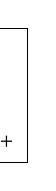
\begin{tikzpicture}[trim axis left, trim axis right]

\begin{axis}[%
width=\figurewidth,
height=\figureheight,
at={(0\figurewidth,0\figureheight)},
scale only axis,
every outer x axis line/.append style={black},
every x tick label/.append style={font=\color{black}},
xmin=9.5,
xmax=16,
xlabel={Time (h)},
every outer y axis line/.append style={black},
every y tick label/.append style={font=\color{black}},
ymin=-0.5,
ymax=0.5,
ylabel={Normalized Book Value},
axis background/.style={fill=white},
axis x line*=bottom,
axis y line*=left,
legend style={legend cell align=left,align=left,draw=black,font=\footnotesize, at={(0.98,0.02)},anchor=south east}
]
\addplot [color=black,solid]
  table[row sep=crcr]{%
9.50027777777778	0\\
9.50583333333333	-0.000231793737116459\\
9.51138888888889	-0.000358042130179537\\
9.51694444444444	-0.000624044133580082\\
9.5225	-0.000704337138179523\\
9.52805555555556	-0.000806368957838699\\
9.53361111111111	-0.000892430694237945\\
9.53916666666667	-0.000668655028491005\\
9.54472222222222	-0.000679814934781309\\
9.55027777777778	-0.000672628843475853\\
9.55583333333333	-0.000745322860736475\\
9.56138888888889	-0.00071655393196346\\
9.56694444444444	-0.000681439299463737\\
9.5725	-0.000695450414574528\\
9.57805555555555	-0.000673883879731663\\
9.58361111111111	-0.000659317409104632\\
9.58916666666667	-0.000621002841693641\\
9.59472222222222	-0.000546146517592216\\
9.60027777777778	-0.000745644539930868\\
9.60583333333333	-0.000766547892410929\\
9.61138888888889	-0.000751569131037688\\
9.61694444444444	-0.000853510681079417\\
9.6225	-0.000831281436831977\\
9.62805555555556	-0.000825117343590587\\
9.63361111111111	-0.000831325026957264\\
9.63916666666667	-0.000804374894810667\\
9.64472222222222	-0.000794067206732141\\
9.65027777777778	-0.000639341901727208\\
9.65583333333333	-0.000606622724905415\\
9.66138888888889	-0.000473285415633407\\
9.66694444444444	-0.000596063833586125\\
9.6725	-0.000464760074997073\\
9.67805555555555	-0.000623819020992622\\
9.68361111111111	-0.000633525944661817\\
9.68916666666667	-0.000444976592099411\\
9.69472222222222	-0.00050328200428873\\
9.70027777777778	-0.000510764229090133\\
9.70583333333333	-0.000720014905398414\\
9.71138888888889	-0.000510787139703539\\
9.71694444444444	-0.000601388040584516\\
9.7225	-0.000510216531229846\\
9.72805555555555	-0.000527103240685611\\
9.73361111111111	-0.000464957574325742\\
9.73916666666667	-0.000414086405420844\\
9.74472222222222	-0.000442162984483963\\
9.75027777777778	-0.000303273727549902\\
9.75583333333333	-0.000319807588345489\\
9.76138888888889	-0.000429585871635108\\
9.76694444444444	-0.000503805162394011\\
9.7725	-0.000438728950765355\\
9.77805555555556	-0.000549918353613399\\
9.78361111111111	-0.000442164634900655\\
9.78916666666667	-0.00054058945893054\\
9.79472222222222	-0.000671441115999816\\
9.80027777777778	-0.000556181514561938\\
9.80583333333333	-0.000553863121377063\\
9.81138888888889	-0.000509252834089091\\
9.81694444444444	-0.000552234080955172\\
9.8225	-0.000548894841679526\\
9.82805555555555	-0.000502966627844881\\
9.83361111111111	-0.00053997615506951\\
9.83916666666667	-0.000563077954824576\\
9.84472222222222	-0.00060496093653184\\
9.85027777777778	-0.000565743244341332\\
9.85583333333333	-0.000441332515205395\\
9.86138888888889	-0.000539759931847072\\
9.86694444444444	-0.000522264980629017\\
9.8725	-0.000508359714266327\\
9.87805555555556	-0.000432992432163659\\
9.88361111111111	-0.000470403210136583\\
9.88916666666667	-0.000440303577289747\\
9.89472222222222	-0.000407402685920766\\
9.90027777777778	-0.000414134063326577\\
9.90583333333333	-0.000397078823199393\\
9.91138888888889	-0.000423827855171921\\
9.91694444444444	-0.000525939230778039\\
9.9225	-0.000511976165591066\\
9.92805555555555	-0.000494488031581475\\
9.93361111111111	-0.000438917341368583\\
9.93916666666667	-0.00038136500767727\\
9.94472222222222	-0.000404726660134691\\
9.95027777777778	-0.000473816892320733\\
9.95583333333333	-0.000452260527121884\\
9.96138888888889	-0.000459018576849046\\
9.96694444444444	-0.000476727516306452\\
9.9725	-0.000478527567585485\\
9.97805555555555	-0.000493796230446208\\
9.98361111111111	-0.000493795472396141\\
9.98916666666667	-0.000563352686366536\\
9.99472222222222	-0.000742969865176413\\
10.0002777777778	-0.000747226491659481\\
10.0058333333333	-0.000682717932618093\\
10.0113888888889	-0.000633298549018391\\
10.0169444444444	-0.000693569143856099\\
10.0225	-0.000636432720171221\\
10.0280555555556	-0.000610508539941157\\
10.0336111111111	-0.000637224163457795\\
10.0391666666667	-0.000816790461895978\\
10.0447222222222	-0.00085027108925062\\
10.0502777777778	-0.000711339738150296\\
10.0558333333333	-0.000715059195751655\\
10.0613888888889	-0.000688495816961177\\
10.0669444444444	-0.000621059112120959\\
10.0725	-0.000637555140431401\\
10.0780555555556	-0.000643652068821887\\
10.0836111111111	-0.000635596714157249\\
10.0891666666667	-0.000589531560579282\\
10.0947222222222	-0.000570172026076454\\
10.1002777777778	-0.000536674809350601\\
10.1058333333333	-0.000582006907978716\\
10.1113888888889	-0.000609715387258736\\
10.1169444444444	-0.0006476608681244\\
10.1225	-0.000636731503331878\\
10.1280555555556	-0.000636755020831825\\
10.1336111111111	-0.000681734295498115\\
10.1391666666667	-0.000697879053012995\\
10.1447222222222	-0.000743194335489084\\
10.1502777777778	-0.000708862488314033\\
10.1558333333333	-0.000755566518815365\\
10.1613888888889	-0.000750778155478637\\
10.1669444444444	-0.000712399374017791\\
10.1725	-0.000704388053086036\\
10.1780555555556	-0.000759592618749361\\
10.1836111111111	-0.00074814059424344\\
10.1891666666667	-0.000762944921240072\\
10.1947222222222	-0.000800253221455827\\
10.2002777777778	-0.000797968884254208\\
10.2058333333333	-0.000838343862346602\\
10.2113888888889	-0.000857952278311092\\
10.2169444444444	-0.000777574673703652\\
10.2225	-0.000796298954289454\\
10.2280555555556	-0.000944208160992943\\
10.2336111111111	-0.000992148137437088\\
10.2391666666667	-0.00101694032544286\\
10.2447222222222	-0.00106373363716361\\
10.2502777777778	-0.00108617682702916\\
10.2558333333333	-0.0010554440018784\\
10.2613888888889	-0.00113364685265971\\
10.2669444444444	-0.00117089929966829\\
10.2725	-0.00123439065111552\\
10.2780555555556	-0.00130108658999972\\
10.2836111111111	-0.00132527443512021\\
10.2891666666667	-0.00131366831755719\\
10.2947222222222	-0.00133170211267486\\
10.3002777777778	-0.00138573070000025\\
10.3058333333333	-0.00149313310410537\\
10.3113888888889	-0.00157028683911364\\
10.3169444444444	-0.00160527957698064\\
10.3225	-0.00160764639324174\\
10.3280555555556	-0.00153539058447671\\
10.3336111111111	-0.00145583774504121\\
10.3391666666667	-0.00147095823672017\\
10.3447222222222	-0.00148318410820325\\
10.3502777777778	-0.00150875880310797\\
10.3558333333333	-0.00153578993183867\\
10.3613888888889	-0.00150993732850968\\
10.3669444444444	-0.00152828643860314\\
10.3725	-0.00152757706891937\\
10.3780555555556	-0.00153490684868596\\
10.3836111111111	-0.00163678758458663\\
10.3891666666667	-0.00171458545238545\\
10.3947222222222	-0.00168106645445942\\
10.4002777777778	-0.00168406225792461\\
10.4058333333333	-0.00163513715915009\\
10.4113888888889	-0.00161125403732254\\
10.4169444444444	-0.00154111718322592\\
10.4225	-0.00154329247963469\\
10.4280555555556	-0.0015665660104669\\
10.4336111111111	-0.00161094524136163\\
10.4391666666667	-0.00166688460384923\\
10.4447222222222	-0.00171716357933516\\
10.4502777777778	-0.00171533201998453\\
10.4558333333333	-0.0017126069164628\\
10.4613888888889	-0.00169750738099772\\
10.4669444444444	-0.00180134039217561\\
10.4725	-0.00179659808634969\\
10.4780555555556	-0.00176947976337227\\
10.4836111111111	-0.00174818512366115\\
10.4891666666667	-0.00172421729367611\\
10.4947222222222	-0.00166623817022238\\
10.5002777777778	-0.0016179276476429\\
10.5058333333333	-0.00164483977840557\\
10.5113888888889	-0.00169228460481041\\
10.5169444444444	-0.00168270671579285\\
10.5225	-0.0017251109882942\\
10.5280555555556	-0.00177011987386777\\
10.5336111111111	-0.00173570920503852\\
10.5391666666667	-0.00172876462084282\\
10.5447222222222	-0.00165735962762759\\
10.5502777777778	-0.00168800209631692\\
10.5558333333333	-0.00173030816757691\\
10.5613888888889	-0.00177893869622936\\
10.5669444444444	-0.00178241765228171\\
10.5725	-0.00176092208989964\\
10.5780555555556	-0.00175880541054851\\
10.5836111111111	-0.00178529382668724\\
10.5891666666667	-0.00175360470523067\\
10.5947222222222	-0.00174975579599601\\
10.6002777777778	-0.00168648050408959\\
10.6058333333333	-0.00167287579947772\\
10.6113888888889	-0.00170936553954903\\
10.6169444444444	-0.00164130172215016\\
10.6225	-0.00162232571126675\\
10.6280555555556	-0.00153011830882621\\
10.6336111111111	-0.00153930355711607\\
10.6391666666667	-0.00151304964870802\\
10.6447222222222	-0.00149347878499939\\
10.6502777777778	-0.00147968555458877\\
10.6558333333333	-0.00145973765876273\\
10.6613888888889	-0.00151885428463827\\
10.6669444444444	-0.00152427600638372\\
10.6725	-0.00145987013887339\\
10.6780555555556	-0.00147278532652673\\
10.6836111111111	-0.0014874089299205\\
10.6891666666667	-0.00143114277035483\\
10.6947222222222	-0.00139891709330464\\
10.7002777777778	-0.00147454734446395\\
10.7058333333333	-0.00147144876777683\\
10.7113888888889	-0.00150990673898954\\
10.7169444444444	-0.00150141254158342\\
10.7225	-0.00148156597143334\\
10.7280555555556	-0.00149982313353025\\
10.7336111111111	-0.00142126398461229\\
10.7391666666667	-0.00136665436657324\\
10.7447222222222	-0.00135205347441714\\
10.7502777777778	-0.00136384386131805\\
10.7558333333333	-0.00130628778851516\\
10.7613888888889	-0.00130188434140011\\
10.7669444444444	-0.00125701662924471\\
10.7725	-0.00123819895788069\\
10.7780555555556	-0.00125213825522563\\
10.7836111111111	-0.00125332190429928\\
10.7891666666667	-0.00122777729959078\\
10.7947222222222	-0.00121946358661718\\
10.8002777777778	-0.00116573600646008\\
10.8058333333333	-0.0011656916382019\\
10.8113888888889	-0.00119731413098778\\
10.8169444444444	-0.0012553643562071\\
10.8225	-0.00123997419350741\\
10.8280555555556	-0.00125045715812155\\
10.8336111111111	-0.00121077540886738\\
10.8391666666667	-0.00124589453076618\\
10.8447222222222	-0.00124192180737026\\
10.8502777777778	-0.00132395274809449\\
10.8558333333333	-0.00129581098396925\\
10.8613888888889	-0.0013176803312599\\
10.8669444444444	-0.00134966722321694\\
10.8725	-0.00137130227346449\\
10.8780555555556	-0.00135385120224429\\
10.8836111111111	-0.00132080722850081\\
10.8891666666667	-0.00130549062930085\\
10.8947222222222	-0.00129746143002119\\
10.9002777777778	-0.00131624601576485\\
10.9058333333333	-0.00132728373171764\\
10.9113888888889	-0.00134397425309618\\
10.9169444444444	-0.00133849823498189\\
10.9225	-0.00134300435255419\\
10.9280555555556	-0.00138634276724103\\
10.9336111111111	-0.00136251249528274\\
10.9391666666667	-0.00133895561592101\\
10.9447222222222	-0.00132999967065184\\
10.9502777777778	-0.00139981718750526\\
10.9558333333333	-0.00139158733985634\\
10.9613888888889	-0.00140211029681903\\
10.9669444444444	-0.00135077332426248\\
10.9725	-0.00135212906169879\\
10.9780555555556	-0.00132221088175222\\
10.9836111111111	-0.0013443121231318\\
10.9891666666667	-0.00142344650309911\\
10.9947222222222	-0.00145904763721949\\
11.0002777777778	-0.00146102629076617\\
11.0058333333333	-0.00140564789975328\\
11.0113888888889	-0.00142708114942114\\
11.0169444444444	-0.00147253614206111\\
11.0225	-0.00147589591716712\\
11.0280555555556	-0.00156097056736493\\
11.0336111111111	-0.00153512196651151\\
11.0391666666667	-0.00151537128365686\\
11.0447222222222	-0.00147996879800782\\
11.0502777777778	-0.00151793109410414\\
11.0558333333333	-0.00152095655735807\\
11.0613888888889	-0.0014840950736752\\
11.0669444444444	-0.00145331752525468\\
11.0725	-0.00143827538507002\\
11.0780555555556	-0.001464242935864\\
11.0836111111111	-0.00145853007785146\\
11.0891666666667	-0.00150118455336368\\
11.0947222222222	-0.00148556024106361\\
11.1002777777778	-0.00152788005296467\\
11.1058333333333	-0.0016096848420013\\
11.1113888888889	-0.00163019175465851\\
11.1169444444444	-0.0015763457146426\\
11.1225	-0.00158003262754369\\
11.1280555555556	-0.00159582682170067\\
11.1336111111111	-0.00160959479232681\\
11.1391666666667	-0.00157620108977141\\
11.1447222222222	-0.00159207558867736\\
11.1502777777778	-0.00167251687301517\\
11.1558333333333	-0.00166966805895208\\
11.1613888888889	-0.00169775585330723\\
11.1669444444444	-0.00172457690905292\\
11.1725	-0.00171182952383719\\
11.1780555555556	-0.00166841946103624\\
11.1836111111111	-0.00170478870117163\\
11.1891666666667	-0.00170052198066761\\
11.1947222222222	-0.00175791914113876\\
11.2002777777778	-0.00172293451179262\\
11.2058333333333	-0.00171379591392473\\
11.2113888888889	-0.00167009819253228\\
11.2169444444444	-0.00172683310845267\\
11.2225	-0.00172478713923552\\
11.2280555555556	-0.0017172127073779\\
11.2336111111111	-0.00170952918422629\\
11.2391666666667	-0.00169528114143236\\
11.2447222222222	-0.00168074672381824\\
11.2502777777778	-0.00172161054908759\\
11.2558333333333	-0.00168996338210969\\
11.2613888888889	-0.0016558303771671\\
11.2669444444444	-0.00166486496694818\\
11.2725	-0.00165889554882681\\
11.2780555555556	-0.00160091728673961\\
11.2836111111111	-0.0015882065551367\\
11.2891666666667	-0.00162778081994741\\
11.2947222222222	-0.00158087651492134\\
11.3002777777778	-0.00157158109877575\\
11.3058333333333	-0.00152789763609884\\
11.3113888888889	-0.00155959845906328\\
11.3169444444444	-0.0015498966591434\\
11.3225	-0.00153061612743932\\
11.3280555555556	-0.0015518567255246\\
11.3336111111111	-0.00158968615464117\\
11.3391666666667	-0.00155374545578046\\
11.3447222222222	-0.00159339536902214\\
11.3502777777778	-0.00157193346946138\\
11.3558333333333	-0.00152361464341089\\
11.3613888888889	-0.00153654195056119\\
11.3669444444444	-0.0015086149639727\\
11.3725	-0.00148346309721048\\
11.3780555555556	-0.00153245904826182\\
11.3836111111111	-0.00147203447125444\\
11.3891666666667	-0.00144841053559475\\
11.3947222222222	-0.00140524047373203\\
11.4002777777778	-0.0014147056547329\\
11.4058333333333	-0.0013987981024759\\
11.4113888888889	-0.00140885399109147\\
11.4169444444444	-0.00140286311282689\\
11.4225	-0.00138573419596999\\
11.4280555555556	-0.00137202799785796\\
11.4336111111111	-0.00136377867263482\\
11.4391666666667	-0.00138586746047953\\
11.4447222222222	-0.00138738801869098\\
11.4502777777778	-0.00139297080029588\\
11.4558333333333	-0.00141258164126745\\
11.4613888888889	-0.00143175055493339\\
11.4669444444444	-0.0014412317092215\\
11.4725	-0.0013879455307807\\
11.4780555555556	-0.00139470479389736\\
11.4836111111111	-0.00141029640125312\\
11.4891666666667	-0.00139514136936281\\
11.4947222222222	-0.00138959770670333\\
11.5002777777778	-0.00139786311584056\\
11.5058333333333	-0.00141203764003917\\
11.5113888888889	-0.00135699676132417\\
11.5169444444444	-0.00125732337961482\\
11.5225	-0.00137775005669516\\
11.5280555555556	-0.00132910780739359\\
11.5336111111111	-0.0012955372717226\\
11.5391666666667	-0.00136161478466368\\
11.5447222222222	-0.00136530652357159\\
11.5502777777778	-0.00133654123632365\\
11.5558333333333	-0.0013022664619704\\
11.5613888888889	-0.00128598626701937\\
11.5669444444444	-0.00122532941858589\\
11.5725	-0.00124378216512211\\
11.5780555555556	-0.00128494090356357\\
11.5836111111111	-0.0013415528438937\\
11.5891666666667	-0.00136339895779403\\
11.5947222222222	-0.00133257239636186\\
11.6002777777778	-0.00139389746490703\\
11.6058333333333	-0.00140335376899403\\
11.6113888888889	-0.00138422221427537\\
11.6169444444444	-0.00143436948945175\\
11.6225	-0.00145971340086215\\
11.6280555555556	-0.00146940066108969\\
11.6336111111111	-0.00148668610441349\\
11.6391666666667	-0.00150143006750003\\
11.6447222222222	-0.00147477830756626\\
11.6502777777778	-0.00140777662591363\\
11.6558333333333	-0.00145394005025723\\
11.6613888888889	-0.00148109521439455\\
11.6669444444444	-0.00146695940805786\\
11.6725	-0.00146992703925153\\
11.6780555555556	-0.00151868926070553\\
11.6836111111111	-0.00152435680190777\\
11.6891666666667	-0.00154555811000945\\
11.6947222222222	-0.00156323114253742\\
11.7002777777778	-0.00153258189660144\\
11.7058333333333	-0.00150489329482728\\
11.7113888888889	-0.00148281087327629\\
11.7169444444444	-0.00152851558983869\\
11.7225	-0.00148980738461979\\
11.7280555555556	-0.0015527731802164\\
11.7336111111111	-0.00153816708386423\\
11.7391666666667	-0.00151339053875488\\
11.7447222222222	-0.00154211169025553\\
11.7502777777778	-0.001569052231015\\
11.7558333333333	-0.00149964017168724\\
11.7613888888889	-0.00153333978524206\\
11.7669444444444	-0.00151558481591207\\
11.7725	-0.00152696928229223\\
11.7780555555556	-0.00150967738659213\\
11.7836111111111	-0.00141585204167483\\
11.7891666666667	-0.00145243745023871\\
11.7947222222222	-0.00144825963536299\\
11.8002777777778	-0.00150162476424553\\
11.8058333333333	-0.00146011959257186\\
11.8113888888889	-0.00144953935213177\\
11.8169444444444	-0.00149637405191372\\
11.8225	-0.00148000585615793\\
11.8280555555556	-0.00146524042907747\\
11.8336111111111	-0.00143050325342697\\
11.8391666666667	-0.00147241768845663\\
11.8447222222222	-0.00145291891378141\\
11.8502777777778	-0.00142846704448529\\
11.8558333333333	-0.00144789769935516\\
11.8613888888889	-0.0014336696603986\\
11.8669444444444	-0.0014063080428236\\
11.8725	-0.00138643204979794\\
11.8780555555556	-0.00135635411074408\\
11.8836111111111	-0.00131093436785978\\
11.8891666666667	-0.00123124921848694\\
11.8947222222222	-0.00124924176198793\\
11.9002777777778	-0.0012765811712443\\
11.9058333333333	-0.00138265424509798\\
11.9113888888889	-0.00138017512436495\\
11.9169444444444	-0.00136816456036037\\
11.9225	-0.0013543315344835\\
11.9280555555556	-0.00133117665615579\\
11.9336111111111	-0.0013015482437958\\
11.9391666666667	-0.00127504355087305\\
11.9447222222222	-0.00122777026421528\\
11.9502777777778	-0.00125982037694017\\
11.9558333333333	-0.00121032819370592\\
11.9613888888889	-0.00126365128416872\\
11.9669444444444	-0.00128160789218923\\
11.9725	-0.00126796943854646\\
11.9780555555556	-0.00121741424373034\\
11.9836111111111	-0.0012139977937442\\
11.9891666666667	-0.00122431010383262\\
11.9947222222222	-0.00127409433169468\\
12.0002777777778	-0.0011875966684527\\
12.0058333333333	-0.00122813029238344\\
12.0113888888889	-0.00119210120527435\\
12.0169444444444	-0.00125596076887113\\
12.0225	-0.00124760592788831\\
12.0280555555556	-0.00126762142573167\\
12.0336111111111	-0.00130121077186152\\
12.0391666666667	-0.00127328753515665\\
12.0447222222222	-0.00130800698716971\\
12.0502777777778	-0.00127681622700804\\
12.0558333333333	-0.00133714458961232\\
12.0613888888889	-0.00136671157840085\\
12.0669444444444	-0.00139374382956525\\
12.0725	-0.00135429012106969\\
12.0780555555556	-0.00133572423542605\\
12.0836111111111	-0.00133953001303033\\
12.0891666666667	-0.00143324542577505\\
12.0947222222222	-0.00144824190743109\\
12.1002777777778	-0.0013972233396301\\
12.1058333333333	-0.00139143182192425\\
12.1113888888889	-0.00139947421762499\\
12.1169444444444	-0.00145315787022804\\
12.1225	-0.00145051068621405\\
12.1280555555556	-0.00148649506126641\\
12.1336111111111	-0.00146776368553969\\
12.1391666666667	-0.00146774824542883\\
12.1447222222222	-0.00149308464426146\\
12.1502777777778	-0.00150721836792067\\
12.1558333333333	-0.00152736308660784\\
12.1613888888889	-0.00149633567593044\\
12.1669444444444	-0.00150273129981293\\
12.1725	-0.00150004120100145\\
12.1780555555556	-0.0015295785575653\\
12.1836111111111	-0.00153310853449751\\
12.1891666666667	-0.00152966814543731\\
12.1947222222222	-0.00149855231290252\\
12.2002777777778	-0.00147823616751896\\
12.2058333333333	-0.00147896649616375\\
12.2113888888889	-0.00147111286492374\\
12.2169444444444	-0.00151516505969529\\
12.2225	-0.00154913100591603\\
12.2280555555556	-0.00152252919921925\\
12.2336111111111	-0.00150228946163278\\
12.2391666666667	-0.00148708829335775\\
12.2447222222222	-0.00142653412658278\\
12.2502777777778	-0.00143813928103864\\
12.2558333333333	-0.00145467710776381\\
12.2613888888889	-0.00146016057534071\\
12.2669444444444	-0.00148525257484133\\
12.2725	-0.00147414089396247\\
12.2780555555556	-0.00145265200606892\\
12.2836111111111	-0.00145913460078462\\
12.2891666666667	-0.00141066735161643\\
12.2947222222222	-0.00138946498071812\\
12.3002777777778	-0.00137166710036019\\
12.3058333333333	-0.00133375678128145\\
12.3113888888889	-0.00131390035469336\\
12.3169444444444	-0.00128484877334556\\
12.3225	-0.00129639560806727\\
12.3280555555556	-0.00128215070212767\\
12.3336111111111	-0.0012965255703058\\
12.3391666666667	-0.001305923249316\\
12.3447222222222	-0.00128146087737369\\
12.3502777777778	-0.0013190214212625\\
12.3558333333333	-0.00134464921541488\\
12.3613888888889	-0.00135135706645828\\
12.3669444444444	-0.00139245321994541\\
12.3725	-0.00132425685024573\\
12.3780555555556	-0.00133704769303444\\
12.3836111111111	-0.00131681633040603\\
12.3891666666667	-0.0013245481229015\\
12.3947222222222	-0.00137704990232557\\
12.4002777777778	-0.00135284215034748\\
12.4058333333333	-0.00132501079205516\\
12.4113888888889	-0.00132427742297359\\
12.4169444444444	-0.00134199655744904\\
12.4225	-0.00134740210310358\\
12.4280555555556	-0.00137679561692572\\
12.4336111111111	-0.00137175724199323\\
12.4391666666667	-0.00137399366344249\\
12.4447222222222	-0.00135851708587487\\
12.4502777777778	-0.0013795251869535\\
12.4558333333333	-0.0014115354112445\\
12.4613888888889	-0.00138728809884681\\
12.4669444444444	-0.00140589561404392\\
12.4725	-0.00142976271636497\\
12.4780555555556	-0.00142027559905622\\
12.4836111111111	-0.00143722188646911\\
12.4891666666667	-0.00134466873437811\\
12.4947222222222	-0.00129548568557869\\
12.5002777777778	-0.00136606218581437\\
12.5058333333333	-0.00134687108000686\\
12.5113888888889	-0.00136807074516432\\
12.5169444444444	-0.00132051171781256\\
12.5225	-0.0012936404618733\\
12.5280555555556	-0.00132701328288376\\
12.5336111111111	-0.00132705262505084\\
12.5391666666667	-0.00132515147226364\\
12.5447222222222	-0.00124941585647209\\
12.5502777777778	-0.0012008677712092\\
12.5558333333333	-0.00123365455324309\\
12.5613888888889	-0.00124733408714162\\
12.5669444444444	-0.00118764790668613\\
12.5725	-0.00112791569780202\\
12.5780555555556	-0.00103883888558387\\
12.5836111111111	-0.00108154332840127\\
12.5891666666667	-0.00102833163123262\\
12.5947222222222	-0.00099301041231481\\
12.6002777777778	-0.00102111655096415\\
12.6058333333333	-0.00103494553351735\\
12.6113888888889	-0.00102925098671114\\
12.6169444444444	-0.00103065143404668\\
12.6225	-0.00103248239507592\\
12.6280555555556	-0.00102372228782865\\
12.6336111111111	-0.00102107584459465\\
12.6391666666667	-0.000999714354949721\\
12.6447222222222	-0.000929042751573572\\
12.6502777777778	-0.00097084824842042\\
12.6558333333333	-0.000945594798557714\\
12.6613888888889	-0.000938783536369892\\
12.6669444444444	-0.000992058703715548\\
12.6725	-0.000886436054219231\\
12.6780555555556	-0.000849732825725424\\
12.6836111111111	-0.000896130318963517\\
12.6891666666667	-0.000917043996663036\\
12.6947222222222	-0.000897544690625196\\
12.7002777777778	-0.000896390415166315\\
12.7058333333333	-0.000857871285157241\\
12.7113888888889	-0.000872691540217296\\
12.7169444444444	-0.000893149805895832\\
12.7225	-0.000865030947968526\\
12.7280555555556	-0.000857690500245867\\
12.7336111111111	-0.00085338126293566\\
12.7391666666667	-0.000857501804570671\\
12.7447222222222	-0.000875099164382998\\
12.7502777777778	-0.000866629576940503\\
12.7558333333333	-0.000923360211912083\\
12.7613888888889	-0.000886256109344341\\
12.7669444444444	-0.000949011013113399\\
12.7725	-0.000984408112574497\\
12.7780555555556	-0.000995835467355377\\
12.7836111111111	-0.000978041448412625\\
12.7891666666667	-0.000923273272620984\\
12.7947222222222	-0.000861153296078609\\
12.8002777777778	-0.000811744814160575\\
12.8058333333333	-0.000771135517302568\\
12.8113888888889	-0.000766352272603577\\
12.8169444444444	-0.000817821617015158\\
12.8225	-0.000831179383467995\\
12.8280555555556	-0.000817754435956664\\
12.8336111111111	-0.000771481861372436\\
12.8391666666667	-0.000806677446545945\\
12.8447222222222	-0.000775752569288746\\
12.8502777777778	-0.000800653848344823\\
12.8558333333333	-0.000769040493637574\\
12.8613888888889	-0.000778406572635282\\
12.8669444444444	-0.000787528175687946\\
12.8725	-0.000771268597614339\\
12.8780555555556	-0.00075843659862318\\
12.8836111111111	-0.000781804529078278\\
12.8891666666667	-0.000805916116337957\\
12.8947222222222	-0.000783954047150814\\
12.9002777777778	-0.000724088526057098\\
12.9058333333333	-0.000726943397987512\\
12.9113888888889	-0.00081927066064702\\
12.9169444444444	-0.000855222880272843\\
12.9225	-0.000816141241411716\\
12.9280555555556	-0.000795430889430015\\
12.9336111111111	-0.000784307308303922\\
12.9391666666667	-0.000797966071879763\\
12.9447222222222	-0.000811328094770358\\
12.9502777777778	-0.000801583959468943\\
12.9558333333333	-0.000768227298502788\\
12.9613888888889	-0.000739439646497808\\
12.9669444444444	-0.000733991899960706\\
12.9725	-0.000692136737565741\\
12.9780555555556	-0.000722755095661665\\
12.9836111111111	-0.000724188116026592\\
12.9891666666667	-0.000734409645590794\\
12.9947222222222	-0.000665890916136114\\
13.0002777777778	-0.000880762856904305\\
13.0058333333333	-0.000893088796747099\\
13.0113888888889	-0.000891256507604132\\
13.0169444444444	-0.000905986170811612\\
13.0225	-0.000902904131966697\\
13.0280555555556	-0.000939876956422614\\
13.0336111111111	-0.000907434400238549\\
13.0391666666667	-0.000925373169094246\\
13.0447222222222	-0.0008973200102802\\
13.0502777777778	-0.000881514560182928\\
13.0558333333333	-0.000841155386032022\\
13.0613888888889	-0.000818141317658116\\
13.0669444444444	-0.000813193552280045\\
13.0725	-0.000755883034038396\\
13.0780555555556	-0.000739125149015307\\
13.0836111111111	-0.000759155594518446\\
13.0891666666667	-0.000734179608488761\\
13.0947222222222	-0.000727824525892262\\
13.1002777777778	-0.000716974159221451\\
13.1058333333333	-0.000731901185583639\\
13.1113888888889	-0.000725622567307793\\
13.1169444444444	-0.000722736170948757\\
13.1225	-0.000697985501624254\\
13.1280555555556	-0.000723445067169703\\
13.1336111111111	-0.000755895492339009\\
13.1391666666667	-0.000733592144611772\\
13.1447222222222	-0.000733994225628143\\
13.1502777777778	-0.000699292646816674\\
13.1558333333333	-0.000751995881791756\\
13.1613888888889	-0.000761311609878579\\
13.1669444444444	-0.000795224078252832\\
13.1725	-0.000807242721475698\\
13.1780555555556	-0.000782783860407532\\
13.1836111111111	-0.000825311927996064\\
13.1891666666667	-0.000797403832400456\\
13.1947222222222	-0.000819928100638023\\
13.2002777777778	-0.000825779601351995\\
13.2058333333333	-0.00084072501522825\\
13.2113888888889	-0.000855781713938963\\
13.2169444444444	-0.000814888914132839\\
13.2225	-0.000782596179180084\\
13.2280555555556	-0.000784391486834513\\
13.2336111111111	-0.000756654701047355\\
13.2391666666667	-0.000765367516353144\\
13.2447222222222	-0.00076756735650263\\
13.2502777777778	-0.000790956703994428\\
13.2558333333333	-0.000791345477523464\\
13.2613888888889	-0.00073163968125356\\
13.2669444444444	-0.000750857891910206\\
13.2725	-0.000733146689698039\\
13.2780555555556	-0.000731483875883066\\
13.2836111111111	-0.000768494180141799\\
13.2891666666667	-0.000801226852823911\\
13.2947222222222	-0.000816765476016945\\
13.3002777777778	-0.000821894220456976\\
13.3058333333333	-0.000870089680503061\\
13.3113888888889	-0.000870592418213523\\
13.3169444444444	-0.000800141361771756\\
13.3225	-0.000804678703719253\\
13.3280555555556	-0.000806685173652788\\
13.3336111111111	-0.000763222459736035\\
13.3391666666667	-0.000760951098592089\\
13.3447222222222	-0.000740920273672008\\
13.3502777777778	-0.000730076326146967\\
13.3558333333333	-0.000750241085710424\\
13.3613888888889	-0.000773830767523354\\
13.3669444444444	-0.00075983990142281\\
13.3725	-0.000750667586721043\\
13.3780555555556	-0.000708439777870606\\
13.3836111111111	-0.000727336784481669\\
13.3891666666667	-0.000706017164548767\\
13.3947222222222	-0.00070972624164789\\
13.4002777777778	-0.000712127357542891\\
13.4058333333333	-0.000763324657780839\\
13.4113888888889	-0.000743098180216784\\
13.4169444444444	-0.000775370494847993\\
13.4225	-0.000801604471813877\\
13.4280555555556	-0.000817447075930899\\
13.4336111111111	-0.0007649550226283\\
13.4391666666667	-0.000744183242297525\\
13.4447222222222	-0.000744365131631008\\
13.4502777777778	-0.000713003886175234\\
13.4558333333333	-0.000754872713205068\\
13.4613888888889	-0.000757053778554062\\
13.4669444444444	-0.00076950468631265\\
13.4725	-0.000783926130787371\\
13.4780555555556	-0.000775929870759251\\
13.4836111111111	-0.000790631442473266\\
13.4891666666667	-0.000803276084516469\\
13.4947222222222	-0.000823607851956121\\
13.5002777777778	-0.000799415562513839\\
13.5058333333333	-0.000794362167035101\\
13.5113888888889	-0.000769725815779165\\
13.5169444444444	-0.000791916335633136\\
13.5225	-0.000827910202000459\\
13.5280555555556	-0.000824521078098495\\
13.5336111111111	-0.000880706604443726\\
13.5391666666667	-0.000844207847943812\\
13.5447222222222	-0.000857821758354249\\
13.5502777777778	-0.000808736892763173\\
13.5558333333333	-0.000817641584635487\\
13.5613888888889	-0.000796394337649664\\
13.5669444444444	-0.000820298795491281\\
13.5725	-0.000828050962069837\\
13.5780555555556	-0.000838861566224147\\
13.5836111111111	-0.000835930481312697\\
13.5891666666667	-0.000825008134958893\\
13.5947222222222	-0.000874321179951676\\
13.6002777777778	-0.000865673810236167\\
13.6058333333333	-0.000908138262671554\\
13.6113888888889	-0.000922955746936793\\
13.6169444444444	-0.000923078021851431\\
13.6225	-0.000898547871010402\\
13.6280555555556	-0.000897604956752951\\
13.6336111111111	-0.000888058413861192\\
13.6391666666667	-0.000922673239127092\\
13.6447222222222	-0.000978636348743289\\
13.6502777777778	-0.000963419610954919\\
13.6558333333333	-0.000954579407484779\\
13.6613888888889	-0.000979314667873932\\
13.6669444444444	-0.000969506520876462\\
13.6725	-0.000952204174828664\\
13.6780555555556	-0.000957251332325937\\
13.6836111111111	-0.000950479169728236\\
13.6891666666667	-0.000930169044787599\\
13.6947222222222	-0.000892229941459433\\
13.7002777777778	-0.000915081781118321\\
13.7058333333333	-0.000930302358073121\\
13.7113888888889	-0.000977699874417093\\
13.7169444444444	-0.000906625848298814\\
13.7225	-0.000926654773821811\\
13.7280555555556	-0.000945448812812888\\
13.7336111111111	-0.0009009862157906\\
13.7391666666667	-0.000905027808887016\\
13.7447222222222	-0.000890288819310858\\
13.7502777777778	-0.000869969545258531\\
13.7558333333333	-0.000918298515835581\\
13.7613888888889	-0.000929661215698152\\
13.7669444444444	-0.000915899230795714\\
13.7725	-0.000934915425896854\\
13.7780555555556	-0.000968322070935557\\
13.7836111111111	-0.00101785122097509\\
13.7891666666667	-0.000989662305204475\\
13.7947222222222	-0.000961344950377696\\
13.8002777777778	-0.000973076153111263\\
13.8058333333333	-0.000932887253212722\\
13.8113888888889	-0.00090327121554401\\
13.8169444444444	-0.000911285379803339\\
13.8225	-0.000910018888000241\\
13.8280555555556	-0.000873412193167167\\
13.8336111111111	-0.000888484275511359\\
13.8391666666667	-0.000879712554306633\\
13.8447222222222	-0.000882621743782508\\
13.8502777777778	-0.000871205086741877\\
13.8558333333333	-0.000847712637590536\\
13.8613888888889	-0.000819191274978093\\
13.8669444444444	-0.000801546669570108\\
13.8725	-0.000824969067725112\\
13.8780555555556	-0.000846725357931399\\
13.8836111111111	-0.00086859706929765\\
13.8891666666667	-0.000855452419997405\\
13.8947222222222	-0.000813236053372357\\
13.9002777777778	-0.000814641942060268\\
13.9058333333333	-0.000832794807409054\\
13.9113888888889	-0.000833610232570892\\
13.9169444444444	-0.000843216181419582\\
13.9225	-0.000852058548136747\\
13.9280555555556	-0.00085934339435445\\
13.9336111111111	-0.000919072532188259\\
13.9391666666667	-0.000929975971765473\\
13.9447222222222	-0.000931599965238061\\
13.9502777777778	-0.00090887206156498\\
13.9558333333333	-0.000885526969452433\\
13.9613888888889	-0.000876752116574564\\
13.9669444444444	-0.000922007673284098\\
13.9725	-0.000902714389181658\\
13.9780555555556	-0.000923752814116274\\
13.9836111111111	-0.000939559038798499\\
13.9891666666667	-0.000950138510526277\\
13.9947222222222	-0.000972705294648324\\
14.0002777777778	-0.000974627201243861\\
14.0058333333333	-0.000931524335986533\\
14.0113888888889	-0.000956917931165591\\
14.0169444444444	-0.000942024167264965\\
14.0225	-0.000991808331958666\\
14.0280555555556	-0.000939534006209386\\
14.0336111111111	-0.000937270073895546\\
14.0391666666667	-0.000943493007879881\\
14.0447222222222	-0.000976272099003195\\
14.0502777777778	-0.000945139405585604\\
14.0558333333333	-0.000959177233612607\\
14.0613888888889	-0.0009390104469299\\
14.0669444444444	-0.000904863817525747\\
14.0725	-0.000931469565164544\\
14.0780555555556	-0.000959799551380147\\
14.0836111111111	-0.000981404480130843\\
14.0891666666667	-0.00095172824487233\\
14.0947222222222	-0.000939192004852929\\
14.1002777777778	-0.000941515074782573\\
14.1058333333333	-0.000959344375947913\\
14.1113888888889	-0.000971714049402439\\
14.1169444444444	-0.000931767282381757\\
14.1225	-0.000944516744454504\\
14.1280555555556	-0.000942889794863677\\
14.1336111111111	-0.000938933072078485\\
14.1391666666667	-0.000947653266787252\\
14.1447222222222	-0.000917198272750941\\
14.1502777777778	-0.000929793945662949\\
14.1558333333333	-0.000953331979810401\\
14.1613888888889	-0.000907308443310439\\
14.1669444444444	-0.000910725392762934\\
14.1725	-0.00091067218813945\\
14.1780555555556	-0.00089133569302835\\
14.1836111111111	-0.000913380195219249\\
14.1891666666667	-0.000919217187533516\\
14.1947222222222	-0.000961312724179431\\
14.2002777777778	-0.000939615451941878\\
14.2058333333333	-0.000850791048497723\\
14.2113888888889	-0.000865370251288855\\
14.2169444444444	-0.000906379787698142\\
14.2225	-0.000931889852143208\\
14.2280555555556	-0.000981500368408161\\
14.2336111111111	-0.000984950959260988\\
14.2391666666667	-0.000974408186733888\\
14.2447222222222	-0.000942976683554253\\
14.2502777777778	-0.000929275367101412\\
14.2558333333333	-0.000849645349276007\\
14.2613888888889	-0.000890716894624832\\
14.2669444444444	-0.000831205439617455\\
14.2725	-0.000835183351104662\\
14.2780555555556	-0.00084815250593484\\
14.2836111111111	-0.000854083731809618\\
14.2891666666667	-0.000781512025652686\\
14.2947222222222	-0.000746125069731707\\
14.3002777777778	-0.000751769294634053\\
14.3058333333333	-0.000755086587570952\\
14.3113888888889	-0.000779311766464508\\
14.3169444444444	-0.000786007455024884\\
14.3225	-0.000794905047811323\\
14.3280555555556	-0.000823448759777134\\
14.3336111111111	-0.000802829696765039\\
14.3391666666667	-0.00085399358266236\\
14.3447222222222	-0.000850442219265557\\
14.3502777777778	-0.000797817423815905\\
14.3558333333333	-0.000789777100734357\\
14.3613888888889	-0.000796081751362254\\
14.3669444444444	-0.000804277074385462\\
14.3725	-0.000832781050224551\\
14.3780555555556	-0.000845975170955415\\
14.3836111111111	-0.000931641777582759\\
14.3891666666667	-0.000896696335034974\\
14.3947222222222	-0.000864384795618789\\
14.4002777777778	-0.000867458810520638\\
14.4058333333333	-0.000846677534686147\\
14.4113888888889	-0.000864392854659335\\
14.4169444444444	-0.000834525327540581\\
14.4225	-0.000802263160829764\\
14.4280555555556	-0.000771925621412262\\
14.4336111111111	-0.000732082366783793\\
14.4391666666667	-0.000761614959560508\\
14.4447222222222	-0.000743067061297231\\
14.4502777777778	-0.000745211110570132\\
14.4558333333333	-0.000811420498405879\\
14.4613888888889	-0.000787490169098737\\
14.4669444444444	-0.000776438446260519\\
14.4725	-0.000774329033453869\\
14.4780555555556	-0.000729813804422386\\
14.4836111111111	-0.00071788169331144\\
14.4891666666667	-0.000688805115670488\\
14.4947222222222	-0.00067018626710158\\
14.5002777777778	-0.000713376420518275\\
14.5058333333333	-0.000720467121745116\\
14.5113888888889	-0.00071044481002569\\
14.5169444444444	-0.000703860787250155\\
14.5225	-0.000679056003980216\\
14.5280555555556	-0.000661040067853835\\
14.5336111111111	-0.000662060441608658\\
14.5391666666667	-0.000641503229247831\\
14.5447222222222	-0.000687257574209732\\
14.5502777777778	-0.000677610941994922\\
14.5558333333333	-0.000668556029144507\\
14.5613888888889	-0.000688893930262058\\
14.5669444444444	-0.000699558463449601\\
14.5725	-0.000689233536389944\\
14.5780555555556	-0.000732476815847205\\
14.5836111111111	-0.000734451606569708\\
14.5891666666667	-0.000715481566144316\\
14.5947222222222	-0.000682553768361127\\
14.6002777777778	-0.000721432521062382\\
14.6058333333333	-0.000733547294996195\\
14.6113888888889	-0.000759961262085218\\
14.6169444444444	-0.000747256343085145\\
14.6225	-0.000718483753800681\\
14.6280555555556	-0.000699252908269332\\
14.6336111111111	-0.000658390854887947\\
14.6391666666667	-0.000694585048392926\\
14.6447222222222	-0.000697457648269117\\
14.6502777777778	-0.000726575219371695\\
14.6558333333333	-0.000772519799196347\\
14.6613888888889	-0.000766612192956928\\
14.6669444444444	-0.00073490524864317\\
14.6725	-0.000770250038339415\\
14.6780555555556	-0.000782616013764725\\
14.6836111111111	-0.000789569478604979\\
14.6891666666667	-0.000749868932496844\\
14.6947222222222	-0.000773514638411354\\
14.7002777777778	-0.000773049693161054\\
14.7058333333333	-0.000787710033599787\\
14.7113888888889	-0.000762787591044534\\
14.7169444444444	-0.00081391818954879\\
14.7225	-0.00077363372094541\\
14.7280555555556	-0.000757502683962352\\
14.7336111111111	-0.000763290526041072\\
14.7391666666667	-0.000746423519751516\\
14.7447222222222	-0.000770246177498657\\
14.7502777777778	-0.000784357734631591\\
14.7558333333333	-0.000776112193211387\\
14.7613888888889	-0.000776360781644225\\
14.7669444444444	-0.00079342107451208\\
14.7725	-0.00078644434846642\\
14.7780555555556	-0.000771334039090243\\
14.7836111111111	-0.000728570635386894\\
14.7891666666667	-0.000716255216802075\\
14.7947222222222	-0.000690898292048603\\
14.8002777777778	-0.000689687101666281\\
14.8058333333333	-0.000705497115836784\\
14.8113888888889	-0.000713917618840543\\
14.8169444444444	-0.000720694216044149\\
14.8225	-0.000724508452544126\\
14.8280555555556	-0.000693259015288938\\
14.8336111111111	-0.000666548039820469\\
14.8391666666667	-0.000662296878381374\\
14.8447222222222	-0.000695917535371349\\
14.8502777777778	-0.000724561183781836\\
14.8558333333333	-0.000670370393457631\\
14.8613888888889	-0.00069463761522337\\
14.8669444444444	-0.000653998504053233\\
14.8725	-0.000712841298411537\\
14.8780555555556	-0.000720371827439892\\
14.8836111111111	-0.000710292565541448\\
14.8891666666667	-0.000698907737670118\\
14.8947222222222	-0.000650564709281154\\
14.9002777777778	-0.000656097330571148\\
14.9058333333333	-0.000695845845207654\\
14.9113888888889	-0.000720992050821434\\
14.9169444444444	-0.000682229438922266\\
14.9225	-0.000690158725149548\\
14.9280555555556	-0.000658537577055807\\
14.9336111111111	-0.000656205061669413\\
14.9391666666667	-0.000615736618507112\\
14.9447222222222	-0.000644163562371292\\
14.9502777777778	-0.00068071594361252\\
14.9558333333333	-0.000689035372611557\\
14.9613888888889	-0.000727125947845408\\
14.9669444444444	-0.000673616313852876\\
14.9725	-0.000684872263432057\\
14.9780555555556	-0.000728187013410708\\
14.9836111111111	-0.000690682942807275\\
14.9891666666667	-0.000662104018542831\\
14.9947222222222	-0.000660102126715523\\
15.0002777777778	-0.000722169163480002\\
15.0058333333333	-0.00074155243393903\\
15.0113888888889	-0.000773265258719236\\
15.0169444444444	-0.000780315673560628\\
15.0225	-0.000792171234575201\\
15.0280555555556	-0.000740077802549699\\
15.0336111111111	-0.000741144952790873\\
15.0391666666667	-0.000790831439186457\\
15.0447222222222	-0.000797266903051153\\
15.0502777777778	-0.000774041277731952\\
15.0558333333333	-0.000771645635563423\\
15.0613888888889	-0.000759254812162991\\
15.0669444444444	-0.000768050318506464\\
15.0725	-0.00076198567326069\\
15.0780555555556	-0.00078477455013326\\
15.0836111111111	-0.000785726999666503\\
15.0891666666667	-0.000737432657445081\\
15.0947222222222	-0.000684043774249132\\
15.1002777777778	-0.000671838373585087\\
15.1058333333333	-0.000745988942030262\\
15.1113888888889	-0.000717194001435995\\
15.1169444444444	-0.00080411711674\\
15.1225	-0.000765878886125448\\
15.1280555555556	-0.000759553169743743\\
15.1336111111111	-0.000826818185269307\\
15.1391666666667	-0.000849812082176493\\
15.1447222222222	-0.000814716663595338\\
15.1502777777778	-0.000836347112174174\\
15.1558333333333	-0.000818738154254373\\
15.1613888888889	-0.000855651010461367\\
15.1669444444444	-0.000843717365753838\\
15.1725	-0.000814874859461745\\
15.1780555555556	-0.000798451556125013\\
15.1836111111111	-0.000785267019975833\\
15.1891666666667	-0.000765040556158891\\
15.1947222222222	-0.000782374837231203\\
15.2002777777778	-0.000809072213043938\\
15.2058333333333	-0.000831312758320601\\
15.2113888888889	-0.00084791443048049\\
15.2169444444444	-0.000787878941839182\\
15.2225	-0.000807149764354365\\
15.2280555555556	-0.000760352184181357\\
15.2336111111111	-0.000790329216791674\\
15.2391666666667	-0.000767178580900918\\
15.2447222222222	-0.000765007723960709\\
15.2502777777778	-0.000762278034621366\\
15.2558333333333	-0.000743718321368547\\
15.2613888888889	-0.000743875528590121\\
15.2669444444444	-0.00072001646485631\\
15.2725	-0.000704984087067206\\
15.2780555555556	-0.000656841052787738\\
15.2836111111111	-0.000628388130713864\\
15.2891666666667	-0.000628776576111156\\
15.2947222222222	-0.000637280158134579\\
15.3002777777778	-0.000668986957623519\\
15.3058333333333	-0.000674299114593491\\
15.3113888888889	-0.000671082528110323\\
15.3169444444444	-0.000621536434402437\\
15.3225	-0.000659585367933091\\
15.3280555555556	-0.00068991420921416\\
15.3336111111111	-0.000735004485263646\\
15.3391666666667	-0.000649487309650532\\
15.3447222222222	-0.000677684581672389\\
15.3502777777778	-0.000708153257196642\\
15.3558333333333	-0.000761535022737236\\
15.3613888888889	-0.000748809288431795\\
15.3669444444444	-0.000756551955936269\\
15.3725	-0.000787695511884623\\
15.3780555555556	-0.000726903149178781\\
15.3836111111111	-0.000714560466251846\\
15.3891666666667	-0.000740602140316349\\
15.3947222222222	-0.000756802475986085\\
15.4002777777778	-0.000769678248804251\\
15.4058333333333	-0.00084526014304831\\
15.4113888888889	-0.000843129771125772\\
15.4169444444444	-0.000834713514815455\\
15.4225	-0.000807091159332085\\
15.4280555555556	-0.000814651775443154\\
15.4336111111111	-0.000830923278634099\\
15.4391666666667	-0.000799399603512274\\
15.4447222222222	-0.000834631243565309\\
15.4502777777778	-0.000767594347568346\\
15.4558333333333	-0.000738915503602722\\
15.4613888888889	-0.000748271849760562\\
15.4669444444444	-0.000719177710275187\\
15.4725	-0.000773657902081726\\
15.4780555555556	-0.000797923581546733\\
15.4836111111111	-0.000790802956902259\\
15.4891666666667	-0.000761112991887414\\
15.4947222222222	-0.000766721063812703\\
15.5002777777778	-0.000776828964460852\\
15.5058333333333	-0.000782402048472242\\
15.5113888888889	-0.000847565438908626\\
15.5169444444444	-0.000832520339935972\\
15.5225	-0.000819613735494884\\
15.5280555555556	-0.000846060110821889\\
15.5336111111111	-0.000827755440233613\\
15.5391666666667	-0.000815439557693476\\
15.5447222222222	-0.000838785074170567\\
15.5502777777778	-0.000795221418902314\\
15.5558333333333	-0.000784401060595297\\
15.5613888888889	-0.000856952479363904\\
15.5669444444444	-0.000867560990537641\\
15.5725	-0.00088596729598367\\
15.5780555555556	-0.00084763377448549\\
15.5836111111111	-0.000855937148092067\\
15.5891666666667	-0.00087428093856623\\
15.5947222222222	-0.000908308658416623\\
15.6002777777778	-0.000894366659356605\\
15.6058333333333	-0.000957350948875169\\
15.6113888888889	-0.000905181426948398\\
15.6169444444444	-0.000913889204942619\\
15.6225	-0.000956003479475886\\
15.6280555555556	-0.000948908213492694\\
15.6336111111111	-0.000947358951854937\\
15.6391666666667	-0.000895027946952287\\
15.6447222222222	-0.000904683205847689\\
15.6502777777778	-0.000908236098068893\\
15.6558333333333	-0.000849439070425673\\
15.6613888888889	-0.000879648706759939\\
15.6669444444444	-0.000932796913614142\\
15.6725	-0.00093359526445147\\
15.6780555555556	-0.000887376838972553\\
15.6836111111111	-0.000899865086301022\\
15.6891666666667	-0.000907917993508867\\
15.6947222222222	-0.000880663256306091\\
15.7002777777778	-0.000901058803943755\\
15.7058333333333	-0.000897178562632939\\
15.7113888888889	-0.000848194727656848\\
15.7169444444444	-0.000888980574435094\\
15.7225	-0.000891043313548834\\
15.7280555555556	-0.00087802367644485\\
15.7336111111111	-0.000891299194873185\\
15.7391666666667	-0.000903019993586662\\
15.7447222222222	-0.000895650039587137\\
15.7502777777778	-0.000870468031698213\\
15.7558333333333	-0.000985574796046218\\
15.7613888888889	-0.00092803187468371\\
15.7669444444444	-0.000893100460505836\\
15.7725	-0.000888162369177214\\
15.7780555555556	-0.000933989695359849\\
15.7836111111111	-0.000950169643745391\\
15.7891666666667	-0.000976510986248402\\
15.7947222222222	-0.000983294242126953\\
15.8002777777778	-0.00089942598181969\\
15.8058333333333	-0.000853691224613207\\
15.8113888888889	-0.000863951896453274\\
15.8169444444444	-0.000910198993857136\\
15.8225	-0.000913591257278301\\
15.8280555555556	-0.000994171077345452\\
15.8336111111111	-0.000900599313715111\\
15.8391666666667	-0.000916956335080155\\
15.8447222222222	-0.000900200042250221\\
15.8502777777778	-0.000925093523531983\\
15.8558333333333	-0.000910593595257359\\
15.8613888888889	-0.00101263840986199\\
15.8669444444444	-0.000945602893104858\\
15.8725	-0.000853098292361132\\
15.8780555555556	-0.000848764268654545\\
15.8836111111111	-0.000781522796555523\\
15.8891666666667	-0.000797602556117383\\
15.8947222222222	-0.000909663346184586\\
15.9002777777778	-0.000874318378281447\\
15.9058333333333	-0.000864250756307139\\
15.9113888888889	-0.000807104782065804\\
15.9169444444444	-0.000698023871892106\\
15.9225	-0.000708423615902509\\
15.9280555555556	-0.0007858702356216\\
15.9336111111111	-0.000743879360312727\\
15.9391666666667	-0.000751234880674967\\
15.9447222222222	-0.000770747185815046\\
15.9502777777778	-0.000798676018124223\\
15.9558333333333	-0.000697209043200364\\
15.9613888888889	-0.000713338873100433\\
15.9669444444444	-0.000672869473814952\\
15.9725	-0.000651654762251708\\
15.9780555555556	-0.000676413284024791\\
15.9836111111111	-0.000682933497711979\\
15.9891666666667	-0.000683933460191799\\
15.9947222222222	-0.000715389861396076\\
};
\addlegendentry{Mid};

\addplot [color=red,solid]
  table[row sep=crcr]{%
9.50027777777778	0\\
9.50583333333333	-0.00640801958033974\\
9.51138888888889	-0.00994323564868329\\
9.51694444444444	-0.0122717926240269\\
9.5225	-0.0147860211247746\\
9.52805555555556	-0.0155781947344845\\
9.53361111111111	-0.017248669219229\\
9.53916666666667	-0.0181244638942349\\
9.54472222222222	-0.0188786788583861\\
9.55027777777778	-0.0197506197994021\\
9.55583333333333	-0.0203486845448715\\
9.56138888888889	-0.020801859379925\\
9.56694444444444	-0.0218585467608209\\
9.5725	-0.023567359476655\\
9.57805555555555	-0.0252881114553215\\
9.58361111111111	-0.0261697169589518\\
9.58916666666667	-0.0275164948642922\\
9.59472222222222	-0.0285838746370957\\
9.60027777777778	-0.0307245885793429\\
9.60583333333333	-0.0322147923056689\\
9.61138888888889	-0.0343209491916611\\
9.61694444444444	-0.0358740026691919\\
9.6225	-0.0371107957267\\
9.62805555555556	-0.0393751174788651\\
9.63361111111111	-0.0402970344529986\\
9.63916666666667	-0.0414914315196692\\
9.64472222222222	-0.0428019253447286\\
9.65027777777778	-0.0421799458954916\\
9.65583333333333	-0.0425997746864147\\
9.66138888888889	-0.0404621494218346\\
9.66694444444444	-0.0453422747123042\\
9.6725	-0.0458381785510247\\
9.67805555555555	-0.049010236775555\\
9.68361111111111	-0.0501058384811373\\
9.68916666666667	-0.0489054702417655\\
9.69472222222222	-0.0504049412742504\\
9.70027777777778	-0.0516038530633764\\
9.70583333333333	-0.0532011759838196\\
9.71138888888889	-0.0540786938732165\\
9.71694444444444	-0.0554826144389037\\
9.7225	-0.0566364872733221\\
9.72805555555555	-0.0574624443161801\\
9.73361111111111	-0.0577298493634292\\
9.73916666666667	-0.0588099238312841\\
9.74472222222222	-0.0596115070652969\\
9.75027777777778	-0.0571940366942688\\
9.75583333333333	-0.0587699862347838\\
9.76138888888889	-0.0610162347974221\\
9.76694444444444	-0.0628636593129067\\
9.7725	-0.0665073313242248\\
9.77805555555556	-0.0682374621774978\\
9.78361111111111	-0.0686112508789999\\
9.78916666666667	-0.0703255607834834\\
9.79472222222222	-0.0754290529145658\\
9.80027777777778	-0.0736531771335652\\
9.80583333333333	-0.0752482250066107\\
9.81138888888889	-0.0753800340789426\\
9.81694444444444	-0.0784298289406945\\
9.8225	-0.0793162987288445\\
9.82805555555555	-0.0795939312346027\\
9.83361111111111	-0.0828739466028884\\
9.83916666666667	-0.0854618078341422\\
9.84472222222222	-0.0870835989197752\\
9.85027777777778	-0.0854289426808013\\
9.85583333333333	-0.0834790581003961\\
9.86138888888889	-0.0858735231073403\\
9.86694444444444	-0.0861092257136162\\
9.8725	-0.0849520331548316\\
9.87805555555556	-0.0843723565344427\\
9.88361111111111	-0.0854026118953056\\
9.88916666666667	-0.0854879841428974\\
9.89472222222222	-0.0859041878505657\\
9.90027777777778	-0.0875066736443845\\
9.90583333333333	-0.0878429695012876\\
9.91138888888889	-0.0891355924277835\\
9.91694444444444	-0.0908973098563148\\
9.9225	-0.0925326673559804\\
9.92805555555555	-0.0934674429827198\\
9.93361111111111	-0.0933103964013502\\
9.93916666666667	-0.0927995975124811\\
9.94472222222222	-0.0918565298658092\\
9.95027777777778	-0.0949829620705606\\
9.95583333333333	-0.0951845274166941\\
9.96138888888889	-0.0961857509419965\\
9.96694444444444	-0.0980718798148505\\
9.9725	-0.0998029066096203\\
9.97805555555555	-0.0994106052974601\\
9.98361111111111	-0.100214031173544\\
9.98916666666667	-0.101713784188367\\
9.99472222222222	-0.106056100429555\\
10.0002777777778	-0.107035878262454\\
10.0058333333333	-0.106949108308114\\
10.0113888888889	-0.106859771755083\\
10.0169444444444	-0.108180466697141\\
10.0225	-0.107406851541173\\
10.0280555555556	-0.104696736236432\\
10.0336111111111	-0.106497545752201\\
10.0391666666667	-0.114515124656075\\
10.0447222222222	-0.116058664679842\\
10.0502777777778	-0.114128741914677\\
10.0558333333333	-0.113935308801159\\
10.0613888888889	-0.115817648069575\\
10.0669444444444	-0.11636479708472\\
10.0725	-0.118026498463266\\
10.0780555555556	-0.118678105463673\\
10.0836111111111	-0.119980082778593\\
10.0891666666667	-0.121707252448748\\
10.0947222222222	-0.121336372410318\\
10.1002777777778	-0.12051328731433\\
10.1058333333333	-0.121423867326925\\
10.1113888888889	-0.12228132288335\\
10.1169444444444	-0.124970203906586\\
10.1225	-0.123261125908866\\
10.1280555555556	-0.122440747890219\\
10.1336111111111	-0.123829384088865\\
10.1391666666667	-0.124454744019786\\
10.1447222222222	-0.126295080484363\\
10.1502777777778	-0.127594194838115\\
10.1558333333333	-0.129897374522266\\
10.1613888888889	-0.127828380099808\\
10.1669444444444	-0.128315074188301\\
10.1725	-0.13011520507876\\
10.1780555555556	-0.132248738641418\\
10.1836111111111	-0.132687619709982\\
10.1891666666667	-0.133797212437082\\
10.1947222222222	-0.134928393132389\\
10.2002777777778	-0.13396316716495\\
10.2058333333333	-0.135090175079464\\
10.2113888888889	-0.136730369983901\\
10.2169444444444	-0.136360819721192\\
10.2225	-0.133987151305363\\
10.2280555555556	-0.136748017428446\\
10.2336111111111	-0.136575933722823\\
10.2391666666667	-0.139426427788202\\
10.2447222222222	-0.142475810422174\\
10.2502777777778	-0.144125002197571\\
10.2558333333333	-0.144182737422554\\
10.2613888888889	-0.14527821932262\\
10.2669444444444	-0.145506283611592\\
10.2725	-0.145002509032252\\
10.2780555555556	-0.147096912735987\\
10.2836111111111	-0.148008337000194\\
10.2891666666667	-0.146965782650649\\
10.2947222222222	-0.147675058735767\\
10.3002777777778	-0.149902805153909\\
10.3058333333333	-0.151611868333779\\
10.3113888888889	-0.153434851224345\\
10.3169444444444	-0.15345894259045\\
10.3225	-0.153400420235121\\
10.3280555555556	-0.154110482369471\\
10.3336111111111	-0.153945811525289\\
10.3391666666667	-0.154054736179588\\
10.3447222222222	-0.153519667371358\\
10.3502777777778	-0.155139925357326\\
10.3558333333333	-0.158447216621139\\
10.3613888888889	-0.158966312119129\\
10.3669444444444	-0.159598099522421\\
10.3725	-0.159372090716639\\
10.3780555555556	-0.160044825951862\\
10.3836111111111	-0.16195130437658\\
10.3891666666667	-0.163671940924239\\
10.3947222222222	-0.162323589968203\\
10.4002777777778	-0.163386184361983\\
10.4058333333333	-0.16249281772678\\
10.4113888888889	-0.162177256390977\\
10.4169444444444	-0.159500799637111\\
10.4225	-0.16039669498445\\
10.4280555555556	-0.162636278055269\\
10.4336111111111	-0.163112346659879\\
10.4391666666667	-0.164371943038481\\
10.4447222222222	-0.165207521523705\\
10.4502777777778	-0.165603191117258\\
10.4558333333333	-0.166304795261924\\
10.4613888888889	-0.164964311812273\\
10.4669444444444	-0.167210331866557\\
10.4725	-0.168865729770178\\
10.4780555555556	-0.16947995014226\\
10.4836111111111	-0.1695300817595\\
10.4891666666667	-0.16968272765968\\
10.4947222222222	-0.170293259889243\\
10.5002777777778	-0.169306581671261\\
10.5058333333333	-0.170374151588671\\
10.5113888888889	-0.172511387849674\\
10.5169444444444	-0.172969658839682\\
10.5225	-0.174798721889475\\
10.5280555555556	-0.17545467760454\\
10.5336111111111	-0.175270125695296\\
10.5391666666667	-0.176155258411028\\
10.5447222222222	-0.174827612529324\\
10.5502777777778	-0.174738662389061\\
10.5558333333333	-0.176551212121828\\
10.5613888888889	-0.176320406281673\\
10.5669444444444	-0.17754842302722\\
10.5725	-0.178222071656096\\
10.5780555555556	-0.178283741552346\\
10.5836111111111	-0.177851422235718\\
10.5891666666667	-0.179006987445043\\
10.5947222222222	-0.178300938973165\\
10.6002777777778	-0.177388155282644\\
10.6058333333333	-0.177745160058271\\
10.6113888888889	-0.182087032985486\\
10.6169444444444	-0.176653793489943\\
10.6225	-0.179473783697027\\
10.6280555555556	-0.176646746010892\\
10.6336111111111	-0.176286439645819\\
10.6391666666667	-0.175771261547777\\
10.6447222222222	-0.174695871631109\\
10.6502777777778	-0.175625592260207\\
10.6558333333333	-0.175858651734311\\
10.6613888888889	-0.178371618991023\\
10.6669444444444	-0.178951804305726\\
10.6725	-0.17745798913585\\
10.6780555555556	-0.178483395477114\\
10.6836111111111	-0.179225253410448\\
10.6891666666667	-0.17893014185687\\
10.6947222222222	-0.176348752602737\\
10.7002777777778	-0.179483720457953\\
10.7058333333333	-0.180354838198796\\
10.7113888888889	-0.181993250401682\\
10.7169444444444	-0.181401931441151\\
10.7225	-0.181332521046519\\
10.7280555555556	-0.18095935902769\\
10.7336111111111	-0.179577883402798\\
10.7391666666667	-0.179282177398789\\
10.7447222222222	-0.180232152226989\\
10.7502777777778	-0.182250081944413\\
10.7558333333333	-0.180531981212436\\
10.7613888888889	-0.18083788597281\\
10.7669444444444	-0.180491086061044\\
10.7725	-0.181929068005786\\
10.7780555555556	-0.182621007211117\\
10.7836111111111	-0.182513865091788\\
10.7891666666667	-0.182325359771756\\
10.7947222222222	-0.182718704558241\\
10.8002777777778	-0.180847457312114\\
10.8058333333333	-0.182389642711163\\
10.8113888888889	-0.18400304296474\\
10.8169444444444	-0.186895587117325\\
10.8225	-0.187066999139384\\
10.8280555555556	-0.185714851773423\\
10.8336111111111	-0.184800746884906\\
10.8391666666667	-0.186337982578089\\
10.8447222222222	-0.186572975019149\\
10.8502777777778	-0.188669827786673\\
10.8558333333333	-0.18749346832209\\
10.8613888888889	-0.189949423876121\\
10.8669444444444	-0.190670534441799\\
10.8725	-0.191117533034421\\
10.8780555555556	-0.190078875108401\\
10.8836111111111	-0.189476949010897\\
10.8891666666667	-0.189432049709199\\
10.8947222222222	-0.189878685635092\\
10.9002777777778	-0.190852720569543\\
10.9058333333333	-0.191547780251347\\
10.9113888888889	-0.1914105862111\\
10.9169444444444	-0.191418056347299\\
10.9225	-0.190714627737159\\
10.9280555555556	-0.193284805635904\\
10.9336111111111	-0.194360943801898\\
10.9391666666667	-0.193889306879152\\
10.9447222222222	-0.195524466508423\\
10.9502777777778	-0.196790415095934\\
10.9558333333333	-0.195640145155287\\
10.9613888888889	-0.197774167826286\\
10.9669444444444	-0.197508996639659\\
10.9725	-0.196934737904351\\
10.9780555555556	-0.197397584089183\\
10.9836111111111	-0.198885904004967\\
10.9891666666667	-0.200287045596615\\
10.9947222222222	-0.200861607213798\\
11.0002777777778	-0.20272172395516\\
11.0058333333333	-0.200738288997222\\
11.0113888888889	-0.200676964755302\\
11.0169444444444	-0.200973991724062\\
11.0225	-0.201712959809955\\
11.0280555555556	-0.202323600372307\\
11.0336111111111	-0.202511317381835\\
11.0391666666667	-0.203066846785891\\
11.0447222222222	-0.204122905891264\\
11.0502777777778	-0.20392266928036\\
11.0558333333333	-0.205129495128911\\
11.0613888888889	-0.205081200450077\\
11.0669444444444	-0.205189143052945\\
11.0725	-0.202891193276187\\
11.0780555555556	-0.2030714260963\\
11.0836111111111	-0.203302499180534\\
11.0891666666667	-0.205085173508928\\
11.0947222222222	-0.204814264513744\\
11.1002777777778	-0.205434476361393\\
11.1058333333333	-0.208102864567999\\
11.1113888888889	-0.207942386447132\\
11.1169444444444	-0.20608803299683\\
11.1225	-0.206054125273972\\
11.1280555555556	-0.208287142874017\\
11.1336111111111	-0.208849574990122\\
11.1391666666667	-0.207606512096596\\
11.1447222222222	-0.20823621251458\\
11.1502777777778	-0.209701897481465\\
11.1558333333333	-0.210720345034446\\
11.1613888888889	-0.211203417993499\\
11.1669444444444	-0.213538473454182\\
11.1725	-0.213978348796847\\
11.1780555555556	-0.212838493166057\\
11.1836111111111	-0.213371113189848\\
11.1891666666667	-0.21315477223775\\
11.1947222222222	-0.217096226936382\\
11.2002777777778	-0.217151430855701\\
11.2058333333333	-0.215860821758135\\
11.2113888888889	-0.214995528712173\\
11.2169444444444	-0.216126285912292\\
11.2225	-0.216689527583645\\
11.2280555555556	-0.217235764833705\\
11.2336111111111	-0.217885061196484\\
11.2391666666667	-0.218941436022406\\
11.2447222222222	-0.218658149854871\\
11.2502777777778	-0.220799650196428\\
11.2558333333333	-0.220066150437702\\
11.2613888888889	-0.219235684408398\\
11.2669444444444	-0.220723815756843\\
11.2725	-0.222009442390514\\
11.2780555555556	-0.22098859217036\\
11.2836111111111	-0.220454333467653\\
11.2891666666667	-0.221464525916891\\
11.2947222222222	-0.219270266227556\\
11.3002777777778	-0.219618722795973\\
11.3058333333333	-0.218412125265291\\
11.3113888888889	-0.219591194989463\\
11.3169444444444	-0.219363805118529\\
11.3225	-0.218613170096463\\
11.3280555555556	-0.219241712840699\\
11.3336111111111	-0.221118455072299\\
11.3391666666667	-0.221140883665122\\
11.3447222222222	-0.222980702032551\\
11.3502777777778	-0.221737549912065\\
11.3558333333333	-0.221209509551754\\
11.3613888888889	-0.221643645680033\\
11.3669444444444	-0.220283439908804\\
11.3725	-0.220742940177824\\
11.3780555555556	-0.22351972766256\\
11.3836111111111	-0.22367808938122\\
11.3891666666667	-0.223061109211673\\
11.3947222222222	-0.222600824795936\\
11.4002777777778	-0.221817649102586\\
11.4058333333333	-0.222597931515101\\
11.4113888888889	-0.222320083597314\\
11.4169444444444	-0.221982287344322\\
11.4225	-0.221603539959705\\
11.4280555555556	-0.222617005589343\\
11.4336111111111	-0.222834651764823\\
11.4391666666667	-0.223595870505493\\
11.4447222222222	-0.224465892134318\\
11.4502777777778	-0.223826579314972\\
11.4558333333333	-0.226053247003428\\
11.4613888888889	-0.226436023080906\\
11.4669444444444	-0.2272078825156\\
11.4725	-0.226986613493023\\
11.4780555555556	-0.22754665776291\\
11.4836111111111	-0.228280517730537\\
11.4891666666667	-0.228228156988719\\
11.4947222222222	-0.228408095681469\\
11.5002777777778	-0.228509390047406\\
11.5058333333333	-0.230141129590446\\
11.5113888888889	-0.231960454577807\\
11.5169444444444	-0.229201578293554\\
11.5225	-0.234611350945744\\
11.5280555555556	-0.231143947878094\\
11.5336111111111	-0.235062273320782\\
11.5391666666667	-0.238605685300073\\
11.5447222222222	-0.238250155157463\\
11.5502777777778	-0.239183998237725\\
11.5558333333333	-0.238697844412845\\
11.5613888888889	-0.238407473960824\\
11.5669444444444	-0.236800400639438\\
11.5725	-0.237737603576985\\
11.5780555555556	-0.239906711621679\\
11.5836111111111	-0.241412448072318\\
11.5891666666667	-0.242338273399491\\
11.5947222222222	-0.24150100284307\\
11.6002777777778	-0.242528245629045\\
11.6058333333333	-0.242788968320804\\
11.6113888888889	-0.244513748580677\\
11.6169444444444	-0.246957740414876\\
11.6225	-0.246442797055627\\
11.6280555555556	-0.246579809091933\\
11.6336111111111	-0.246255041609757\\
11.6391666666667	-0.246071234743353\\
11.6447222222222	-0.245493442491321\\
11.6502777777778	-0.2440591810118\\
11.6558333333333	-0.243852025829463\\
11.6613888888889	-0.245031870312832\\
11.6669444444444	-0.245843695272152\\
11.6725	-0.246709585677105\\
11.6780555555556	-0.247610205270583\\
11.6836111111111	-0.247858802708386\\
11.6891666666667	-0.251014611483473\\
11.6947222222222	-0.251924984967679\\
11.7002777777778	-0.252260941644505\\
11.7058333333333	-0.25382073525713\\
11.7113888888889	-0.255480825707666\\
11.7169444444444	-0.257046191712778\\
11.7225	-0.256048020976306\\
11.7280555555556	-0.258930774191084\\
11.7336111111111	-0.259858957433236\\
11.7391666666667	-0.25846058405052\\
11.7447222222222	-0.260895257414198\\
11.7502777777778	-0.262081711942855\\
11.7558333333333	-0.259231548317907\\
11.7613888888889	-0.260201649148654\\
11.7669444444444	-0.258236278987139\\
11.7725	-0.259351491117067\\
11.7780555555556	-0.260180705754291\\
11.7836111111111	-0.258992976392051\\
11.7891666666667	-0.260848176796563\\
11.7947222222222	-0.260840887071224\\
11.8002777777778	-0.26325695677462\\
11.8058333333333	-0.262694328180974\\
11.8113888888889	-0.263576028122331\\
11.8169444444444	-0.266474298520711\\
11.8225	-0.266177942598479\\
11.8280555555556	-0.266332947736641\\
11.8336111111111	-0.266013885852449\\
11.8391666666667	-0.268031874520845\\
11.8447222222222	-0.26699572635656\\
11.8502777777778	-0.267058781946418\\
11.8558333333333	-0.268130758062746\\
11.8613888888889	-0.268500432093892\\
11.8669444444444	-0.267874010643115\\
11.8725	-0.268270572422842\\
11.8780555555556	-0.267891773378785\\
11.8836111111111	-0.267603949598858\\
11.8891666666667	-0.26577659476872\\
11.8947222222222	-0.266852498210848\\
11.9002777777778	-0.266828952203278\\
11.9058333333333	-0.272287871559834\\
11.9113888888889	-0.273708064196298\\
11.9169444444444	-0.271200796108949\\
11.9225	-0.270453423754553\\
11.9280555555556	-0.271811150620119\\
11.9336111111111	-0.271321412122556\\
11.9391666666667	-0.270314737965356\\
11.9447222222222	-0.2686214197905\\
11.9502777777778	-0.271541404274342\\
11.9558333333333	-0.271859450155028\\
11.9613888888889	-0.2736055704081\\
11.9669444444444	-0.273551813004795\\
11.9725	-0.274007310597594\\
11.9780555555556	-0.272627476495626\\
11.9836111111111	-0.273937859104292\\
11.9891666666667	-0.274677922563928\\
11.9947222222222	-0.277436326910911\\
12.0002777777778	-0.275845627569173\\
12.0058333333333	-0.276490611836336\\
12.0113888888889	-0.273732423175889\\
12.0169444444444	-0.275858705987663\\
12.0225	-0.2757190516737\\
12.0280555555556	-0.276488056580881\\
12.0336111111111	-0.276045729025001\\
12.0391666666667	-0.275652771375364\\
12.0447222222222	-0.275951832417152\\
12.0502777777778	-0.275032007885572\\
12.0558333333333	-0.27701528736462\\
12.0613888888889	-0.278516257497256\\
12.0669444444444	-0.278966741941133\\
12.0725	-0.27683294711088\\
12.0780555555556	-0.277196396307465\\
12.0836111111111	-0.277169528382678\\
12.0891666666667	-0.279062962841671\\
12.0947222222222	-0.280029608731538\\
12.1002777777778	-0.27974800283096\\
12.1058333333333	-0.278874574744513\\
12.1113888888889	-0.277798226315694\\
12.1169444444444	-0.27904339215099\\
12.1225	-0.279357239826403\\
12.1280555555556	-0.282281530899528\\
12.1336111111111	-0.283130674832874\\
12.1391666666667	-0.283084947118419\\
12.1447222222222	-0.284169205709224\\
12.1502777777778	-0.284258040688714\\
12.1558333333333	-0.285987295962158\\
12.1613888888889	-0.285648234379712\\
12.1669444444444	-0.28459043855587\\
12.1725	-0.283342614322316\\
12.1780555555556	-0.28412655458624\\
12.1836111111111	-0.284140831186778\\
12.1891666666667	-0.283783461594809\\
12.1947222222222	-0.28249666323897\\
12.2002777777778	-0.281528703253455\\
12.2058333333333	-0.282351864233898\\
12.2113888888889	-0.282987964334292\\
12.2169444444444	-0.285047184783045\\
12.2225	-0.286978163546681\\
12.2280555555556	-0.287344837007631\\
12.2336111111111	-0.286257908393567\\
12.2391666666667	-0.287109365405827\\
12.2447222222222	-0.284222774647802\\
12.2502777777778	-0.284461202232336\\
12.2558333333333	-0.282604020572015\\
12.2613888888889	-0.2846415804635\\
12.2669444444444	-0.285583652158306\\
12.2725	-0.286555467576085\\
12.2780555555556	-0.288281599627282\\
12.2836111111111	-0.290539047718813\\
12.2891666666667	-0.288278904360436\\
12.2947222222222	-0.287674800915548\\
12.3002777777778	-0.289004481430947\\
12.3058333333333	-0.289522433389963\\
12.3113888888889	-0.28987637814162\\
12.3169444444444	-0.288344052373989\\
12.3225	-0.288819418636382\\
12.3280555555556	-0.289283238813881\\
12.3336111111111	-0.288858270627228\\
12.3391666666667	-0.288318316295821\\
12.3447222222222	-0.286691314939739\\
12.3502777777778	-0.288226743260326\\
12.3558333333333	-0.289917758628696\\
12.3613888888889	-0.290347190041068\\
12.3669444444444	-0.293268350260158\\
12.3725	-0.29077294944781\\
12.3780555555556	-0.292020084149683\\
12.3836111111111	-0.29281472629108\\
12.3891666666667	-0.292159803954428\\
12.3947222222222	-0.294867764541812\\
12.4002777777778	-0.295403271007182\\
12.4058333333333	-0.295698014536883\\
12.4113888888889	-0.295740016941035\\
12.4169444444444	-0.298685232666795\\
12.4225	-0.299331830321968\\
12.4280555555556	-0.301359770058987\\
12.4336111111111	-0.299570017696773\\
12.4391666666667	-0.299722490837734\\
12.4447222222222	-0.300317956675159\\
12.4502777777778	-0.300879369961282\\
12.4558333333333	-0.301898170880896\\
12.4613888888889	-0.301202859088241\\
12.4669444444444	-0.302309383303941\\
12.4725	-0.303156880181555\\
12.4780555555556	-0.302530482115583\\
12.4836111111111	-0.303465007476794\\
12.4891666666667	-0.30158943479147\\
12.4947222222222	-0.300283212278939\\
12.5002777777778	-0.30110998655564\\
12.5058333333333	-0.301605035091408\\
12.5113888888889	-0.303781975944825\\
12.5169444444444	-0.305085487907025\\
12.5225	-0.305281916556464\\
12.5280555555556	-0.306806262772947\\
12.5336111111111	-0.306423656616942\\
12.5391666666667	-0.306177077423248\\
12.5447222222222	-0.305605626705354\\
12.5502777777778	-0.303988129421797\\
12.5558333333333	-0.306078568869503\\
12.5613888888889	-0.306480434509078\\
12.5669444444444	-0.304410691191638\\
12.5725	-0.30177440291658\\
12.5780555555556	-0.297829067990861\\
12.5836111111111	-0.300421385678577\\
12.5891666666667	-0.300021661876721\\
12.5947222222222	-0.301064321284544\\
12.6002777777778	-0.300562146416569\\
12.6058333333333	-0.30121067111367\\
12.6113888888889	-0.303787112191239\\
12.6169444444444	-0.303996965810326\\
12.6225	-0.305540181151464\\
12.6280555555556	-0.304994756566121\\
12.6336111111111	-0.303456746852192\\
12.6391666666667	-0.303707597073752\\
12.6447222222222	-0.301771061691515\\
12.6502777777778	-0.303383707843853\\
12.6558333333333	-0.303650202627512\\
12.6613888888889	-0.304935286258932\\
12.6669444444444	-0.306041265780505\\
12.6725	-0.302927707766606\\
12.6780555555556	-0.302281179903812\\
12.6836111111111	-0.303314314778712\\
12.6891666666667	-0.304480182647648\\
12.6947222222222	-0.30438404110731\\
12.7002777777778	-0.304715234105437\\
12.7058333333333	-0.305339011698499\\
12.7113888888889	-0.306330702076282\\
12.7169444444444	-0.307205602136059\\
12.7225	-0.306334589957786\\
12.7280555555556	-0.308564266872462\\
12.7336111111111	-0.308141044245202\\
12.7391666666667	-0.30832467833607\\
12.7447222222222	-0.309270369268929\\
12.7502777777778	-0.310217153437485\\
12.7558333333333	-0.313588777932575\\
12.7613888888889	-0.310564058145869\\
12.7669444444444	-0.314743429510141\\
12.7725	-0.316509811371806\\
12.7780555555556	-0.317389194714838\\
12.7836111111111	-0.317357290151483\\
12.7891666666667	-0.31386228932076\\
12.7947222222222	-0.312394846524613\\
12.8002777777778	-0.309143930380493\\
12.8058333333333	-0.30817549032464\\
12.8113888888889	-0.310297608449103\\
12.8169444444444	-0.312047262621866\\
12.8225	-0.312873417698119\\
12.8280555555556	-0.314951321174505\\
12.8336111111111	-0.312331109130694\\
12.8391666666667	-0.312626311282716\\
12.8447222222222	-0.311708516660224\\
12.8502777777778	-0.312059645287935\\
12.8558333333333	-0.311237662771026\\
12.8613888888889	-0.310123671654506\\
12.8669444444444	-0.309610561793655\\
12.8725	-0.309352614833251\\
12.8780555555556	-0.309926394499545\\
12.8836111111111	-0.313004433323855\\
12.8891666666667	-0.312556277082707\\
12.8947222222222	-0.311983825289022\\
12.9002777777778	-0.313246753415582\\
12.9058333333333	-0.312060282205201\\
12.9113888888889	-0.316638089862064\\
12.9169444444444	-0.316977436654226\\
12.9225	-0.314492268623972\\
12.9280555555556	-0.314061337354777\\
12.9336111111111	-0.314662713222566\\
12.9391666666667	-0.315770023067952\\
12.9447222222222	-0.31569219718418\\
12.9502777777778	-0.315508529621835\\
12.9558333333333	-0.315484729847628\\
12.9613888888889	-0.316677142132733\\
12.9669444444444	-0.31760110756094\\
12.9725	-0.316781611423601\\
12.9780555555556	-0.318071645731304\\
12.9836111111111	-0.319545790070622\\
12.9891666666667	-0.321968733750667\\
12.9947222222222	-0.320822347018727\\
13.0002777777778	-0.315995227470025\\
13.0058333333333	-0.31610019601627\\
13.0113888888889	-0.31681062764022\\
13.0169444444444	-0.317467260674241\\
13.0225	-0.315776018971422\\
13.0280555555556	-0.318597067044082\\
13.0336111111111	-0.318075560163999\\
13.0391666666667	-0.31802339823317\\
13.0447222222222	-0.316678992945926\\
13.0502777777778	-0.316372013543664\\
13.0558333333333	-0.315184990960401\\
13.0613888888889	-0.31415305008965\\
13.0669444444444	-0.314121021856804\\
13.0725	-0.313116127970486\\
13.0780555555556	-0.312090212614219\\
13.0836111111111	-0.312242441933564\\
13.0891666666667	-0.311896150789059\\
13.0947222222222	-0.312799472542906\\
13.1002777777778	-0.312943950344332\\
13.1058333333333	-0.312524079618739\\
13.1113888888889	-0.312661347187189\\
13.1169444444444	-0.313211940041088\\
13.1225	-0.3145012348071\\
13.1280555555556	-0.314526523544639\\
13.1336111111111	-0.315706158659845\\
13.1391666666667	-0.314738170583914\\
13.1447222222222	-0.315361798790835\\
13.1502777777778	-0.313835658302943\\
13.1558333333333	-0.315527869388553\\
13.1613888888889	-0.316065993325718\\
13.1669444444444	-0.317663384999949\\
13.1725	-0.317307514521323\\
13.1780555555556	-0.317544969658959\\
13.1836111111111	-0.319580000203398\\
13.1891666666667	-0.318959903126439\\
13.1947222222222	-0.318990281078342\\
13.2002777777778	-0.318337169750948\\
13.2058333333333	-0.317539951214669\\
13.2113888888889	-0.318465201432754\\
13.2169444444444	-0.317365240886028\\
13.2225	-0.317558853181345\\
13.2280555555556	-0.317358417083445\\
13.2336111111111	-0.316372686450573\\
13.2391666666667	-0.316729513081786\\
13.2447222222222	-0.316181527225838\\
13.2502777777778	-0.314720197853122\\
13.2558333333333	-0.315678826042001\\
13.2613888888889	-0.313727950413204\\
13.2669444444444	-0.313602295565264\\
13.2725	-0.313343910134501\\
13.2780555555556	-0.314782373685807\\
13.2836111111111	-0.318030647688162\\
13.2891666666667	-0.31888416965843\\
13.2947222222222	-0.320823208118068\\
13.3002777777778	-0.321141897214271\\
13.3058333333333	-0.322657161762819\\
13.3113888888889	-0.321461837378985\\
13.3169444444444	-0.316378748731817\\
13.3225	-0.315676411184345\\
13.3280555555556	-0.315388205095351\\
13.3336111111111	-0.313806623494076\\
13.3391666666667	-0.315282077897033\\
13.3447222222222	-0.313881632241939\\
13.3502777777778	-0.313557207696487\\
13.3558333333333	-0.314462257355836\\
13.3613888888889	-0.315622630611755\\
13.3669444444444	-0.315079285362939\\
13.3725	-0.315027105405459\\
13.3780555555556	-0.313381391415909\\
13.3836111111111	-0.312816691249062\\
13.3891666666667	-0.313337539951643\\
13.3947222222222	-0.314828612930865\\
13.4002777777778	-0.315616629986771\\
13.4058333333333	-0.315221856478531\\
13.4113888888889	-0.312863056369206\\
13.4169444444444	-0.312547896394416\\
13.4225	-0.313284974583885\\
13.4280555555556	-0.312856570958651\\
13.4336111111111	-0.310206336934621\\
13.4391666666667	-0.30920943309373\\
13.4447222222222	-0.309347259823854\\
13.4502777777778	-0.309675934724386\\
13.4558333333333	-0.311098083055322\\
13.4613888888889	-0.311363806972277\\
13.4669444444444	-0.313161540687044\\
13.4725	-0.314122386882832\\
13.4780555555556	-0.313786593923502\\
13.4836111111111	-0.314253690479447\\
13.4891666666667	-0.314262243840376\\
13.4947222222222	-0.315382226800749\\
13.5002777777778	-0.314774600012298\\
13.5058333333333	-0.315116928013729\\
13.5113888888889	-0.313195525038752\\
13.5169444444444	-0.314578769035284\\
13.5225	-0.314795281220923\\
13.5280555555556	-0.313288802851328\\
13.5336111111111	-0.322564649476283\\
13.5391666666667	-0.3212457027706\\
13.5447222222222	-0.321445491643082\\
13.5502777777778	-0.319916810731737\\
13.5558333333333	-0.321185069759451\\
13.5613888888889	-0.323966028145783\\
13.5669444444444	-0.324470892199856\\
13.5725	-0.325106930105236\\
13.5780555555556	-0.32692185144679\\
13.5836111111111	-0.328429084683651\\
13.5891666666667	-0.325947104554187\\
13.5947222222222	-0.333782132980604\\
13.6002777777778	-0.331317391015434\\
13.6058333333333	-0.332901579176876\\
13.6113888888889	-0.334056902268125\\
13.6169444444444	-0.333992416253903\\
13.6225	-0.335396732639813\\
13.6280555555556	-0.336201546497696\\
13.6336111111111	-0.338181203126413\\
13.6391666666667	-0.339555426696321\\
13.6447222222222	-0.340293919657894\\
13.6502777777778	-0.340647235479405\\
13.6558333333333	-0.341712087101079\\
13.6613888888889	-0.341615591629928\\
13.6669444444444	-0.339989603922546\\
13.6725	-0.340113285388844\\
13.6780555555556	-0.343383805688717\\
13.6836111111111	-0.341943925921088\\
13.6891666666667	-0.342824760962956\\
13.6947222222222	-0.343269057845293\\
13.7002777777778	-0.344728198095511\\
13.7058333333333	-0.34289066820687\\
13.7113888888889	-0.344429787014366\\
13.7169444444444	-0.342965043397993\\
13.7225	-0.342498972717885\\
13.7280555555556	-0.34306910101403\\
13.7336111111111	-0.342583153901771\\
13.7391666666667	-0.341990295486366\\
13.7447222222222	-0.342279880454447\\
13.7502777777778	-0.343826211290857\\
13.7558333333333	-0.34299700739603\\
13.7613888888889	-0.3426721962216\\
13.7669444444444	-0.343094212550775\\
13.7725	-0.342773295848196\\
13.7780555555556	-0.344903149232433\\
13.7836111111111	-0.344293089463866\\
13.7891666666667	-0.345361471360246\\
13.7947222222222	-0.347745813982669\\
13.8002777777778	-0.346874968876972\\
13.8058333333333	-0.346309025537207\\
13.8113888888889	-0.346601880519931\\
13.8169444444444	-0.346868839250101\\
13.8225	-0.348657601021791\\
13.8280555555556	-0.347782356836718\\
13.8336111111111	-0.348125219018703\\
13.8391666666667	-0.34557325219961\\
13.8447222222222	-0.345519977512802\\
13.8502777777778	-0.345758206916445\\
13.8558333333333	-0.346161816747851\\
13.8613888888889	-0.344878227324962\\
13.8669444444444	-0.346002144488481\\
13.8725	-0.345634815676312\\
13.8780555555556	-0.345933243998752\\
13.8836111111111	-0.34624379838789\\
13.8891666666667	-0.34559074340223\\
13.8947222222222	-0.341360585138739\\
13.9002777777778	-0.341536070878916\\
13.9058333333333	-0.343753576734574\\
13.9113888888889	-0.341101844475683\\
13.9169444444444	-0.343088471276734\\
13.9225	-0.345273477563753\\
13.9280555555556	-0.347032279601712\\
13.9336111111111	-0.349705778109878\\
13.9391666666667	-0.349870125733341\\
13.9447222222222	-0.3483688768885\\
13.9502777777778	-0.346875016037867\\
13.9558333333333	-0.3473154324234\\
13.9613888888889	-0.350318137290456\\
13.9669444444444	-0.351542975836508\\
13.9725	-0.348498529387218\\
13.9780555555556	-0.350218208720357\\
13.9836111111111	-0.350181121071133\\
13.9891666666667	-0.351004655270581\\
13.9947222222222	-0.35315093566679\\
14.0002777777778	-0.354744080356465\\
14.0058333333333	-0.355491162702908\\
14.0113888888889	-0.356370152151515\\
14.0169444444444	-0.353962904331367\\
14.0225	-0.353018731761638\\
14.0280555555556	-0.353035514892884\\
14.0336111111111	-0.356684423435816\\
14.0391666666667	-0.352265316157037\\
14.0447222222222	-0.351726538108443\\
14.0502777777778	-0.349548654418258\\
14.0558333333333	-0.3490104814258\\
14.0613888888889	-0.347740787882463\\
14.0669444444444	-0.345485111924748\\
14.0725	-0.350166773639972\\
14.0780555555556	-0.351713072398017\\
14.0836111111111	-0.350591959959082\\
14.0891666666667	-0.349609137150345\\
14.0947222222222	-0.351745676439118\\
14.1002777777778	-0.350211924735604\\
14.1058333333333	-0.349536054028614\\
14.1113888888889	-0.347740520294457\\
14.1169444444444	-0.346947776599847\\
14.1225	-0.344952179803821\\
14.1280555555556	-0.343570177713962\\
14.1336111111111	-0.345246579761122\\
14.1391666666667	-0.346233775959657\\
14.1447222222222	-0.347874842774746\\
14.1502777777778	-0.349575012852997\\
14.1558333333333	-0.350940600702464\\
14.1613888888889	-0.348664965512548\\
14.1669444444444	-0.349429009276126\\
14.1725	-0.350371237516819\\
14.1780555555556	-0.350939394563992\\
14.1836111111111	-0.354516548491318\\
14.1891666666667	-0.354548921174021\\
14.1947222222222	-0.362182796604674\\
14.2002777777778	-0.361359401297002\\
14.2058333333333	-0.356767929254566\\
14.2113888888889	-0.359905166384632\\
14.2169444444444	-0.362198213842413\\
14.2225	-0.364559695076565\\
14.2280555555556	-0.367745067676475\\
14.2336111111111	-0.36978695752505\\
14.2391666666667	-0.370098444446208\\
14.2447222222222	-0.369699949497301\\
14.2502777777778	-0.369175748918117\\
14.2558333333333	-0.363810563328182\\
14.2613888888889	-0.365149205319755\\
14.2669444444444	-0.364969420339875\\
14.2725	-0.363426547625828\\
14.2780555555556	-0.364710473224079\\
14.2836111111111	-0.364572428353398\\
14.2891666666667	-0.363348697642911\\
14.2947222222222	-0.361104333471136\\
14.3002777777778	-0.362271929958343\\
14.3058333333333	-0.360671905817368\\
14.3113888888889	-0.363824761616734\\
14.3169444444444	-0.363448465654387\\
14.3225	-0.365144079213609\\
14.3280555555556	-0.36572366576533\\
14.3336111111111	-0.365417699008696\\
14.3391666666667	-0.36888159623523\\
14.3447222222222	-0.367890281967555\\
14.3502777777778	-0.371683831405721\\
14.3558333333333	-0.372190922249969\\
14.3613888888889	-0.372720037102174\\
14.3669444444444	-0.373489821371826\\
14.3725	-0.374928575449489\\
14.3780555555556	-0.374885471889921\\
14.3836111111111	-0.380159094602111\\
14.3891666666667	-0.378305590486148\\
14.3947222222222	-0.377073894561118\\
14.4002777777778	-0.379444991129049\\
14.4058333333333	-0.378993009736867\\
14.4113888888889	-0.378111428068494\\
14.4169444444444	-0.379471870850093\\
14.4225	-0.381619462571137\\
14.4280555555556	-0.379946087267515\\
14.4336111111111	-0.376830222584596\\
14.4391666666667	-0.377893084215183\\
14.4447222222222	-0.380080999902544\\
14.4502777777778	-0.381935606077083\\
14.4558333333333	-0.386672935982321\\
14.4613888888889	-0.385572910898569\\
14.4669444444444	-0.385536617737622\\
14.4725	-0.382302612362641\\
14.4780555555556	-0.380767088306518\\
14.4836111111111	-0.380183988158339\\
14.4891666666667	-0.37951966233448\\
14.4947222222222	-0.380326676541365\\
14.5002777777778	-0.381577514838767\\
14.5058333333333	-0.380892174241959\\
14.5113888888889	-0.382059068680702\\
14.5169444444444	-0.379952847444939\\
14.5225	-0.378880684977433\\
14.5280555555556	-0.378427285124149\\
14.5336111111111	-0.375815267334659\\
14.5391666666667	-0.374867944653697\\
14.5447222222222	-0.380076705210335\\
14.5502777777778	-0.381116613689984\\
14.5558333333333	-0.382197586753108\\
14.5613888888889	-0.383395690822203\\
14.5669444444444	-0.386630122383891\\
14.5725	-0.384704346267087\\
14.5780555555556	-0.388344574397647\\
14.5836111111111	-0.389031825808536\\
14.5891666666667	-0.387983045476291\\
14.5947222222222	-0.38182372541388\\
14.6002777777778	-0.384058091801518\\
14.6058333333333	-0.38398859057943\\
14.6113888888889	-0.385349596446785\\
14.6169444444444	-0.385419710957053\\
14.6225	-0.382653077421884\\
14.6280555555556	-0.383632042187205\\
14.6336111111111	-0.381384489603691\\
14.6391666666667	-0.382304351962839\\
14.6447222222222	-0.384939901025729\\
14.6502777777778	-0.38566291553231\\
14.6558333333333	-0.389273564531108\\
14.6613888888889	-0.387898636536061\\
14.6669444444444	-0.38722664970724\\
14.6725	-0.386870245086344\\
14.6780555555556	-0.38521526838468\\
14.6836111111111	-0.389384195971318\\
14.6891666666667	-0.387845348513425\\
14.6947222222222	-0.390356137945901\\
14.7002777777778	-0.392386380305283\\
14.7058333333333	-0.393803028041546\\
14.7113888888889	-0.393431409400749\\
14.7169444444444	-0.395582074787325\\
14.7225	-0.39439472800498\\
14.7280555555556	-0.394902990863272\\
14.7336111111111	-0.390471533253438\\
14.7391666666667	-0.386979784191519\\
14.7447222222222	-0.389539000019681\\
14.7502777777778	-0.390012673297053\\
14.7558333333333	-0.391102652995097\\
14.7613888888889	-0.3968729719647\\
14.7669444444444	-0.398557244691672\\
14.7725	-0.398802561213067\\
14.7780555555556	-0.397888974657029\\
14.7836111111111	-0.396677166210794\\
14.7891666666667	-0.395297844114016\\
14.7947222222222	-0.39513962749402\\
14.8002777777778	-0.398150444231352\\
14.8058333333333	-0.396258828097851\\
14.8113888888889	-0.396549579018369\\
14.8169444444444	-0.396027613043553\\
14.8225	-0.395838460191955\\
14.8280555555556	-0.391798504903928\\
14.8336111111111	-0.391082052002772\\
14.8391666666667	-0.390631669554883\\
14.8447222222222	-0.392193579468822\\
14.8502777777778	-0.400281791439257\\
14.8558333333333	-0.393358578510891\\
14.8613888888889	-0.395582880858089\\
14.8669444444444	-0.39625598982362\\
14.8725	-0.398319793813763\\
14.8780555555556	-0.400423313601924\\
14.8836111111111	-0.399955999305032\\
14.8891666666667	-0.400245521258263\\
14.8947222222222	-0.399626727050718\\
14.9002777777778	-0.401186714185812\\
14.9058333333333	-0.399569076663933\\
14.9113888888889	-0.401926959236324\\
14.9169444444444	-0.398312971577858\\
14.9225	-0.399771018990461\\
14.9280555555556	-0.400226966692175\\
14.9336111111111	-0.400702953716785\\
14.9391666666667	-0.400640842024087\\
14.9447222222222	-0.403034109331713\\
14.9502777777778	-0.408074993537048\\
14.9558333333333	-0.408553269495268\\
14.9613888888889	-0.410028392676575\\
14.9669444444444	-0.408227996748311\\
14.9725	-0.415037897765753\\
14.9780555555556	-0.416336856112493\\
14.9836111111111	-0.414489135707217\\
14.9891666666667	-0.417131651645196\\
14.9947222222222	-0.415542620629534\\
15.0002777777778	-0.415618893603369\\
15.0058333333333	-0.419715003754787\\
15.0113888888889	-0.420185005550877\\
15.0169444444444	-0.421229047020427\\
15.0225	-0.418690521266783\\
15.0280555555556	-0.412040503124556\\
15.0336111111111	-0.414368524211509\\
15.0391666666667	-0.420459831456875\\
15.0447222222222	-0.424416818536359\\
15.0502777777778	-0.423516066325519\\
15.0558333333333	-0.420700031223872\\
15.0613888888889	-0.422881203482914\\
15.0669444444444	-0.426456947224232\\
15.0725	-0.431341542794747\\
15.0780555555556	-0.427117069348786\\
15.0836111111111	-0.428812157458962\\
15.0891666666667	-0.41995008336028\\
15.0947222222222	-0.417780210663047\\
15.1002777777778	-0.424158854978147\\
15.1058333333333	-0.425675366351245\\
15.1113888888889	-0.423067010694157\\
15.1169444444444	-0.428414281298974\\
15.1225	-0.428832149748332\\
15.1280555555556	-0.426589235968319\\
15.1336111111111	-0.438249532139913\\
15.1391666666667	-0.438425912179304\\
15.1447222222222	-0.43355015824645\\
15.1502777777778	-0.433410014235992\\
15.1558333333333	-0.428939182991526\\
15.1613888888889	-0.432103317711764\\
15.1669444444444	-0.430887354583178\\
15.1725	-0.427975479247256\\
15.1780555555556	-0.429636457437925\\
15.1836111111111	-0.430323795186837\\
15.1891666666667	-0.428994474231948\\
15.1947222222222	-0.431196239530814\\
15.2002777777778	-0.434042984622807\\
15.2058333333333	-0.436573688329312\\
15.2113888888889	-0.436866846274045\\
15.2169444444444	-0.43478021939483\\
15.2225	-0.436221650179893\\
15.2280555555556	-0.437148739141597\\
15.2336111111111	-0.441442279848913\\
15.2391666666667	-0.440457440164333\\
15.2447222222222	-0.441725828750769\\
15.2502777777778	-0.441792592628797\\
15.2558333333333	-0.440115896051457\\
15.2613888888889	-0.44024826718053\\
15.2669444444444	-0.438895332644953\\
15.2725	-0.440121639821355\\
15.2780555555556	-0.436273046613611\\
15.2836111111111	-0.436059272391379\\
15.2891666666667	-0.438095032430995\\
15.2947222222222	-0.43780080473577\\
15.3002777777778	-0.440394041797217\\
15.3058333333333	-0.440957419220693\\
15.3113888888889	-0.439274123038672\\
15.3169444444444	-0.438933494858749\\
15.3225	-0.441590854382077\\
15.3280555555556	-0.443954992994061\\
15.3336111111111	-0.446344047994773\\
15.3391666666667	-0.441046707967388\\
15.3447222222222	-0.441919535239238\\
15.3502777777778	-0.442648412798371\\
15.3558333333333	-0.445724791261675\\
15.3613888888889	-0.443238485118724\\
15.3669444444444	-0.443976775532498\\
15.3725	-0.44366347002539\\
15.3780555555556	-0.443011256678291\\
15.3836111111111	-0.441537612784522\\
15.3891666666667	-0.441931081180907\\
15.3947222222222	-0.442124527956484\\
15.4002777777778	-0.443921310396545\\
15.4058333333333	-0.443613191077505\\
15.4113888888889	-0.444502863356461\\
15.4169444444444	-0.447402219442775\\
15.4225	-0.448038238077684\\
15.4280555555556	-0.450670882395055\\
15.4336111111111	-0.451466096455659\\
15.4391666666667	-0.450623232059456\\
15.4447222222222	-0.45032952428868\\
15.4502777777778	-0.442784849536023\\
15.4558333333333	-0.441632732694759\\
15.4613888888889	-0.441723854642445\\
15.4669444444444	-0.444413856989371\\
15.4725	-0.447619449144359\\
15.4780555555556	-0.447835728097767\\
15.4836111111111	-0.447015455013771\\
15.4891666666667	-0.444780371390743\\
15.4947222222222	-0.446269637110884\\
15.5002777777778	-0.444330426953079\\
15.5058333333333	-0.446541116579177\\
15.5113888888889	-0.447578166259094\\
15.5169444444444	-0.448883160888707\\
15.5225	-0.450253459445227\\
15.5280555555556	-0.454775836922221\\
15.5336111111111	-0.452753333636565\\
15.5391666666667	-0.451860780013068\\
15.5447222222222	-0.452760669997031\\
15.5502777777778	-0.449799378845893\\
15.5558333333333	-0.451058878913738\\
15.5613888888889	-0.450358104919822\\
15.5669444444444	-0.449155581628101\\
15.5725	-0.45012150451954\\
15.5780555555556	-0.449353404366591\\
15.5836111111111	-0.446318321439556\\
15.5891666666667	-0.451492083690042\\
15.5947222222222	-0.452808239186564\\
15.6002777777778	-0.455111529841579\\
15.6058333333333	-0.458516993111177\\
15.6113888888889	-0.459477461046019\\
15.6169444444444	-0.460398133689201\\
15.6225	-0.465480137718923\\
15.6280555555556	-0.46813058876681\\
15.6336111111111	-0.471160223969854\\
15.6391666666667	-0.469638233700124\\
15.6447222222222	-0.468252730220178\\
15.6502777777778	-0.470902704882154\\
15.6558333333333	-0.467954825716294\\
15.6613888888889	-0.468154066819365\\
15.6669444444444	-0.472231308261287\\
15.6725	-0.4725572938238\\
15.6780555555556	-0.469531302722083\\
15.6836111111111	-0.471273497001529\\
15.6891666666667	-0.472968875312938\\
15.6947222222222	-0.472819518682729\\
15.7002777777778	-0.470372713991943\\
15.7058333333333	-0.470905941031454\\
15.7113888888889	-0.472279983672575\\
15.7169444444444	-0.474863068065271\\
15.7225	-0.476543104621414\\
15.7280555555556	-0.473276492074349\\
15.7336111111111	-0.475483842506897\\
15.7391666666667	-0.476635379470553\\
15.7447222222222	-0.476766379685005\\
15.7502777777778	-0.470091628055338\\
15.7558333333333	-0.475520697517352\\
15.7613888888889	-0.472425118946259\\
15.7669444444444	-0.471842681722525\\
15.7725	-0.471988598487372\\
15.7780555555556	-0.473955348160659\\
15.7836111111111	-0.474848958431833\\
15.7891666666667	-0.481001963654947\\
15.7947222222222	-0.481336282606231\\
15.8002777777778	-0.480858654992737\\
15.8058333333333	-0.480493940599718\\
15.8113888888889	-0.48167628187952\\
15.8169444444444	-0.482283361924387\\
15.8225	-0.478494763802247\\
15.8280555555556	-0.479878684431253\\
15.8336111111111	-0.483784127257366\\
15.8391666666667	-0.479594173611283\\
15.8447222222222	-0.479674028759197\\
15.8502777777778	-0.482517774356702\\
15.8558333333333	-0.482035409429657\\
15.8613888888889	-0.484867236568923\\
15.8669444444444	-0.484330029251771\\
15.8725	-0.485334436587639\\
15.8780555555556	-0.487999677899215\\
15.8836111111111	-0.486368186265838\\
15.8891666666667	-0.484448003381359\\
15.8947222222222	-0.489916373389079\\
15.9002777777778	-0.492929236514484\\
15.9058333333333	-0.495526802719254\\
15.9113888888889	-0.491252090933643\\
15.9169444444444	-0.482129846113552\\
15.9225	-0.481682684124339\\
15.9280555555556	-0.481057999237424\\
15.9336111111111	-0.483317397500689\\
15.9391666666667	-0.480834878634586\\
15.9447222222222	-0.4787634463385\\
15.9502777777778	-0.475567487060841\\
15.9558333333333	-0.479889836478797\\
15.9613888888889	-0.48260201356166\\
15.9669444444444	-0.48069537745755\\
15.9725	-0.484075567015736\\
15.9780555555556	-0.484555787788874\\
15.9836111111111	-0.482243529314598\\
15.9891666666667	-0.483017790466192\\
15.9947222222222	-0.486220333294028\\
};
\addlegendentry{Naive};

\addplot [color=blue,solid]
  table[row sep=crcr]{%
9.50027777777778	0\\
9.50583333333333	0.00114109851543311\\
9.51138888888889	0.00174598168067803\\
9.51694444444444	0.00189201305740803\\
9.5225	0.00233029587111862\\
9.52805555555556	0.00296786744390659\\
9.53361111111111	0.00317848619845286\\
9.53916666666667	0.00319053694721352\\
9.54472222222222	0.00371091998464402\\
9.55027777777778	0.00308650037488377\\
9.55583333333333	0.00328404942029467\\
9.56138888888889	0.00400080779165284\\
9.56694444444444	0.00521479122515946\\
9.5725	0.0055418940159534\\
9.57805555555555	0.00567506417446694\\
9.58361111111111	0.00587077835833908\\
9.58916666666667	0.00584014329557747\\
9.59472222222222	0.00593512297862885\\
9.60027777777778	0.00549977075544583\\
9.60583333333333	0.00590283278130339\\
9.61138888888889	0.0051905667566488\\
9.61694444444444	0.00584634480305781\\
9.6225	0.00621270995779072\\
9.62805555555556	0.00587914138849719\\
9.63361111111111	0.00617723997810902\\
9.63916666666667	0.00646533503808321\\
9.64472222222222	0.00557617597992557\\
9.65027777777778	0.00690902248259715\\
9.65583333333333	0.00573259399400813\\
9.66138888888889	0.00501866415361975\\
9.66694444444444	0.00557360844141024\\
9.6725	0.00674479309513822\\
9.67805555555555	0.00572547506191342\\
9.68361111111111	0.00533158247995932\\
9.68916666666667	0.00536303423031648\\
9.69472222222222	0.00459147581653035\\
9.70027777777778	0.00629276420816819\\
9.70583333333333	0.00680822278824667\\
9.71138888888889	0.00808103851474408\\
9.71694444444444	0.00848300435542191\\
9.7225	0.00891539520163241\\
9.72805555555555	0.00983023623964303\\
9.73361111111111	0.0103864892085915\\
9.73916666666667	0.0103168854659793\\
9.74472222222222	0.00947521699070127\\
9.75027777777778	0.00906507962743727\\
9.75583333333333	0.00939416599051953\\
9.76138888888889	0.00941435331161418\\
9.76694444444444	0.00870800702979264\\
9.7725	0.00884715504238784\\
9.77805555555556	0.00978692521605999\\
9.78361111111111	0.0100883316754734\\
9.78916666666667	0.0106440879653555\\
9.79472222222222	0.0110908564480651\\
9.80027777777778	0.0109797342172152\\
9.80583333333333	0.0110979029053312\\
9.81138888888889	0.0116271052875279\\
9.81694444444444	0.0115596250395176\\
9.8225	0.0118591929800556\\
9.82805555555555	0.0112016344608721\\
9.83361111111111	0.0113511201390018\\
9.83916666666667	0.011913615638644\\
9.84472222222222	0.011290628666508\\
9.85027777777778	0.0132653111123824\\
9.85583333333333	0.0143349378170579\\
9.86138888888889	0.0126081748188242\\
9.86694444444444	0.0141927231276852\\
9.8725	0.0151423208951139\\
9.87805555555556	0.0148007432217365\\
9.88361111111111	0.0149284560443661\\
9.88916666666667	0.0152239129229428\\
9.89472222222222	0.0156196369002608\\
9.90027777777778	0.0145048027745437\\
9.90583333333333	0.0143031509189139\\
9.91138888888889	0.0152655522056701\\
9.91694444444444	0.0138984580135961\\
9.9225	0.0149272460587219\\
9.92805555555555	0.0149508758422215\\
9.93361111111111	0.0150496623524819\\
9.93916666666667	0.0152631373744863\\
9.94472222222222	0.014900397279493\\
9.95027777777778	0.0145350233988047\\
9.95583333333333	0.0149842646042938\\
9.96138888888889	0.0141555251476175\\
9.96694444444444	0.0140206171386777\\
9.9725	0.014402118101235\\
9.97805555555555	0.0144776156715456\\
9.98361111111111	0.0142320073984748\\
9.98916666666667	0.014057743318928\\
9.99472222222222	0.0143145200014963\\
10.0002777777778	0.0158703647328059\\
10.0058333333333	0.0168504948235333\\
10.0113888888889	0.0169060007479373\\
10.0169444444444	0.0173807935472452\\
10.0225	0.0175850253881828\\
10.0280555555556	0.0182431878189408\\
10.0336111111111	0.0179094191910992\\
10.0391666666667	0.0166520044517598\\
10.0447222222222	0.0175100318993099\\
10.0502777777778	0.0177554029113355\\
10.0558333333333	0.0183913420665915\\
10.0613888888889	0.0183548271158244\\
10.0669444444444	0.0183449242031594\\
10.0725	0.018538797702462\\
10.0780555555556	0.0187453355380593\\
10.0836111111111	0.0188026980944874\\
10.0891666666667	0.0187794983412617\\
10.0947222222222	0.0190539093742014\\
10.1002777777778	0.0187120276686433\\
10.1058333333333	0.0193397783957299\\
10.1113888888889	0.0208893669941548\\
10.1169444444444	0.0197445006859441\\
10.1225	0.0206761345623606\\
10.1280555555556	0.0216069793236775\\
10.1336111111111	0.0222353354185069\\
10.1391666666667	0.0222813499272309\\
10.1447222222222	0.0221876523589595\\
10.1502777777778	0.0225715233220321\\
10.1558333333333	0.0229230083454668\\
10.1613888888889	0.0229879068504181\\
10.1669444444444	0.022443224069474\\
10.1725	0.0223937759384182\\
10.1780555555556	0.0226089706633995\\
10.1836111111111	0.0229559970770589\\
10.1891666666667	0.0206612951269011\\
10.1947222222222	0.0206161280821994\\
10.2002777777778	0.0216788933766209\\
10.2058333333333	0.0215551276531368\\
10.2113888888889	0.0217976512986175\\
10.2169444444444	0.022346536641948\\
10.2225	0.0229415089994438\\
10.2280555555556	0.0219457318702635\\
10.2336111111111	0.0225365975498804\\
10.2391666666667	0.0230009299479874\\
10.2447222222222	0.0222886266328922\\
10.2502777777778	0.021315962391892\\
10.2558333333333	0.0214574840287462\\
10.2613888888889	0.0240697936900849\\
10.2669444444444	0.0243752722243358\\
10.2725	0.0243743908640682\\
10.2780555555556	0.0233871347336631\\
10.2836111111111	0.0243181742967493\\
10.2891666666667	0.0237344765865385\\
10.2947222222222	0.022712270540856\\
10.3002777777778	0.0214715386151555\\
10.3058333333333	0.0212339124993487\\
10.3113888888889	0.0222860096531903\\
10.3169444444444	0.0224279471447947\\
10.3225	0.0216334538421045\\
10.3280555555556	0.0224038912822312\\
10.3336111111111	0.0236491794830045\\
10.3391666666667	0.0230486653745044\\
10.3447222222222	0.0231625605965897\\
10.3502777777778	0.0218499126653826\\
10.3558333333333	0.0214832281956403\\
10.3613888888889	0.0223561077684799\\
10.3669444444444	0.0199371213889198\\
10.3725	0.0201620960803728\\
10.3780555555556	0.017193740723456\\
10.3836111111111	0.019586010103146\\
10.3891666666667	0.020181682522182\\
10.3947222222222	0.0196231222896877\\
10.4002777777778	0.017958511835463\\
10.4058333333333	0.0175673045183135\\
10.4113888888889	0.0191556097822171\\
10.4169444444444	0.0213386313083682\\
10.4225	0.0218158846495942\\
10.4280555555556	0.0213700854646378\\
10.4336111111111	0.0200284052274311\\
10.4391666666667	0.0189107183001789\\
10.4447222222222	0.0237822097244945\\
10.4502777777778	0.0215493515178342\\
10.4558333333333	0.0221430797246002\\
10.4613888888889	0.022689511126621\\
10.4669444444444	0.0232847537422505\\
10.4725	0.0234149828722959\\
10.4780555555556	0.0227343842352191\\
10.4836111111111	0.0222227482299537\\
10.4891666666667	0.0218445029606153\\
10.4947222222222	0.0231058393904182\\
10.5002777777778	0.0237965818152145\\
10.5058333333333	0.0239546452349267\\
10.5113888888889	0.0233460801785989\\
10.5169444444444	0.0258762653633217\\
10.5225	0.0251728108231245\\
10.5280555555556	0.0224988298533553\\
10.5336111111111	0.0221728768829677\\
10.5391666666667	0.0255478416274611\\
10.5447222222222	0.0253345999837597\\
10.5502777777778	0.0255405459530237\\
10.5558333333333	0.0258497486731386\\
10.5613888888889	0.0253825293258671\\
10.5669444444444	0.0254006830862331\\
10.5725	0.0273364608764364\\
10.5780555555556	0.0278661578365936\\
10.5836111111111	0.0305066746266632\\
10.5891666666667	0.0291904077506581\\
10.5947222222222	0.0294724864214857\\
10.6002777777778	0.0298112905213267\\
10.6058333333333	0.031033910054369\\
10.6113888888889	0.0312397987161375\\
10.6169444444444	0.0318269223982955\\
10.6225	0.0324746006201653\\
10.6280555555556	0.0336008444520065\\
10.6336111111111	0.0334615224525741\\
10.6391666666667	0.0351638632630682\\
10.6447222222222	0.0362763853968546\\
10.6502777777778	0.0372880909013886\\
10.6558333333333	0.0354015937192471\\
10.6613888888889	0.0357743548417029\\
10.6669444444444	0.0351881864893065\\
10.6725	0.0356072087121007\\
10.6780555555556	0.0352153083795645\\
10.6836111111111	0.0351404981216761\\
10.6891666666667	0.0354230878463727\\
10.6947222222222	0.0351130697717186\\
10.7002777777778	0.0351105388313493\\
10.7058333333333	0.0349828595725922\\
10.7113888888889	0.0352908864884097\\
10.7169444444444	0.0356170126821349\\
10.7225	0.0351808964006029\\
10.7280555555556	0.0348026954783251\\
10.7336111111111	0.0349695066101859\\
10.7391666666667	0.0354006080956076\\
10.7447222222222	0.0351059756994466\\
10.7502777777778	0.0350697282467652\\
10.7558333333333	0.0356738952445968\\
10.7613888888889	0.0366067420611834\\
10.7669444444444	0.0364433190848289\\
10.7725	0.0371229679804979\\
10.7780555555556	0.0363765135100389\\
10.7836111111111	0.0361412935925859\\
10.7891666666667	0.0361550687683979\\
10.7947222222222	0.0353800330891688\\
10.8002777777778	0.0362652747532407\\
10.8058333333333	0.0348792775503673\\
10.8113888888889	0.0351143361824128\\
10.8169444444444	0.0353020226917463\\
10.8225	0.0352918323039161\\
10.8280555555556	0.0329413438542764\\
10.8336111111111	0.0329626455839795\\
10.8391666666667	0.0323805030921435\\
10.8447222222222	0.0338874716620125\\
10.8502777777778	0.0340792367000217\\
10.8558333333333	0.0349847751467005\\
10.8613888888889	0.0348614509805065\\
10.8669444444444	0.0345050073510973\\
10.8725	0.0348388874983041\\
10.8780555555556	0.035079693076504\\
10.8836111111111	0.0355787083439044\\
10.8891666666667	0.03606467346288\\
10.8947222222222	0.0358051597547103\\
10.9002777777778	0.0360163144538666\\
10.9058333333333	0.0339996867062015\\
10.9113888888889	0.0337208066029817\\
10.9169444444444	0.0347044787533061\\
10.9225	0.0348060355534862\\
10.9280555555556	0.0339633469511773\\
10.9336111111111	0.0334284729075521\\
10.9391666666667	0.0338492247036758\\
10.9447222222222	0.0331350019616834\\
10.9502777777778	0.033307158298198\\
10.9558333333333	0.0326538788820229\\
10.9613888888889	0.0332436012360675\\
10.9669444444444	0.0338062145109597\\
10.9725	0.0344928278170008\\
10.9780555555556	0.0330552595724996\\
10.9836111111111	0.0324900159983978\\
10.9891666666667	0.0325545592433863\\
10.9947222222222	0.0321091220469581\\
11.0002777777778	0.0310382008182824\\
11.0058333333333	0.0309370278055323\\
11.0113888888889	0.0275928253304246\\
11.0169444444444	0.0274282784008425\\
11.0225	0.0277190367918428\\
11.0280555555556	0.0293752262152213\\
11.0336111111111	0.0318328943754336\\
11.0391666666667	0.0310447775926197\\
11.0447222222222	0.0318900212418978\\
11.0502777777778	0.03267644482899\\
11.0558333333333	0.032604199214863\\
11.0613888888889	0.0321994374750379\\
11.0669444444444	0.0326033619276198\\
11.0725	0.0333787124614772\\
11.0780555555556	0.0332386732293026\\
11.0836111111111	0.0348522331006492\\
11.0891666666667	0.0348951506663447\\
11.0947222222222	0.0353233500963176\\
11.1002777777778	0.0352129897851402\\
11.1058333333333	0.0350186415482685\\
11.1113888888889	0.0336759375949916\\
11.1169444444444	0.0343078750256963\\
11.1225	0.0353625322257787\\
11.1280555555556	0.0350115404744079\\
11.1336111111111	0.0351715264090371\\
11.1391666666667	0.0359796542960048\\
11.1447222222222	0.0347868585755245\\
11.1502777777778	0.0350253347933622\\
11.1558333333333	0.0347271060052366\\
11.1613888888889	0.0343518104394191\\
11.1669444444444	0.0323533301269215\\
11.1725	0.0315644365106291\\
11.1780555555556	0.0326390070511437\\
11.1836111111111	0.0325957789079772\\
11.1891666666667	0.0319920029824361\\
11.1947222222222	0.0317240770291782\\
11.2002777777778	0.0312453605451851\\
11.2058333333333	0.0313960879613751\\
11.2113888888889	0.0307033197209497\\
11.2169444444444	0.0312488429446432\\
11.2225	0.0314405964027414\\
11.2280555555556	0.0319032547108317\\
11.2336111111111	0.0321459502787302\\
11.2391666666667	0.0315051715988079\\
11.2447222222222	0.031115688740961\\
11.2502777777778	0.0297649057258483\\
11.2558333333333	0.0277025442620851\\
11.2613888888889	0.026751199781224\\
11.2669444444444	0.0274869339719585\\
11.2725	0.0266752586448408\\
11.2780555555556	0.0268133519321917\\
11.2836111111111	0.0270016820530274\\
11.2891666666667	0.0264067250243241\\
11.2947222222222	0.0263818299304646\\
11.3002777777778	0.0224225243210405\\
11.3058333333333	0.0229058244907695\\
11.3113888888889	0.0241268190415795\\
11.3169444444444	0.0290620400921386\\
11.3225	0.0284619487976224\\
11.3280555555556	0.0273081015643287\\
11.3336111111111	0.0289021885074299\\
11.3391666666667	0.0295304157737336\\
11.3447222222222	0.0303883182251731\\
11.3502777777778	0.0317252192574492\\
11.3558333333333	0.0322379957776059\\
11.3613888888889	0.0335567341093273\\
11.3669444444444	0.0329705594663734\\
11.3725	0.034391028319187\\
11.3780555555556	0.0339533015127026\\
11.3836111111111	0.0322889323047372\\
11.3891666666667	0.0325550533534452\\
11.3947222222222	0.0326556982815772\\
11.4002777777778	0.0331728215602066\\
11.4058333333333	0.0335702951557751\\
11.4113888888889	0.0337798153550739\\
11.4169444444444	0.0342471195040469\\
11.4225	0.0339107725070873\\
11.4280555555556	0.0327896056156529\\
11.4336111111111	0.0326341518113574\\
11.4391666666667	0.0319842316305677\\
11.4447222222222	0.0319343590536177\\
11.4502777777778	0.0324259978340235\\
11.4558333333333	0.0334467296106629\\
11.4613888888889	0.0340140196991796\\
11.4669444444444	0.0351425435958243\\
11.4725	0.0343272293900448\\
11.4780555555556	0.0348593010580453\\
11.4836111111111	0.0357367892873023\\
11.4891666666667	0.0352159593477048\\
11.4947222222222	0.0342228451544923\\
11.5002777777778	0.0334086597517523\\
11.5058333333333	0.0340314050716316\\
11.5113888888889	0.0342888488705933\\
11.5169444444444	0.0346748250772081\\
11.5225	0.0341901047063594\\
11.5280555555556	0.0344663214782268\\
11.5336111111111	0.0334912437140005\\
11.5391666666667	0.0332205315693642\\
11.5447222222222	0.0336338315467742\\
11.5502777777778	0.0337733818987157\\
11.5558333333333	0.0346972444466607\\
11.5613888888889	0.0341181915747659\\
11.5669444444444	0.0349602180864125\\
11.5725	0.033890117905741\\
11.5780555555556	0.0314290542726349\\
11.5836111111111	0.0304830087391625\\
11.5891666666667	0.0304602957134416\\
11.5947222222222	0.0310503365679847\\
11.6002777777778	0.0327023111970614\\
11.6058333333333	0.0318550050029165\\
11.6113888888889	0.0312555932197502\\
11.6169444444444	0.03207282329915\\
11.6225	0.0322312138261481\\
11.6280555555556	0.0344057909062407\\
11.6336111111111	0.0340584354348413\\
11.6391666666667	0.0343943756488418\\
11.6447222222222	0.0351955380179576\\
11.6502777777778	0.0355434850417402\\
11.6558333333333	0.0372718284767132\\
11.6613888888889	0.0382644105406287\\
11.6669444444444	0.0371163779418274\\
11.6725	0.0355597627860893\\
11.6780555555556	0.0352893625889084\\
11.6836111111111	0.0364606590313644\\
11.6891666666667	0.0359285009797298\\
11.6947222222222	0.0370105960428862\\
11.7002777777778	0.0363064455231425\\
11.7058333333333	0.034514187837848\\
11.7113888888889	0.0343299947893674\\
11.7169444444444	0.0337019347893585\\
11.7225	0.0346644908048503\\
11.7280555555556	0.0332215482460833\\
11.7336111111111	0.0340621997569317\\
11.7391666666667	0.0340757228777793\\
11.7447222222222	0.0347913308541177\\
11.7502777777778	0.0341125434448994\\
11.7558333333333	0.0349678091885297\\
11.7613888888889	0.0342146598146039\\
11.7669444444444	0.0354666803888858\\
11.7725	0.035530090088253\\
11.7780555555556	0.0337161996947103\\
11.7836111111111	0.0331963421795001\\
11.7891666666667	0.032485371610329\\
11.7947222222222	0.0318760590581886\\
11.8002777777778	0.030431670443827\\
11.8058333333333	0.0312809867324293\\
11.8113888888889	0.0299794144282876\\
11.8169444444444	0.02958264413143\\
11.8225	0.0298116053036682\\
11.8280555555556	0.0302398488095471\\
11.8336111111111	0.0292522365987001\\
11.8391666666667	0.0297171943778931\\
11.8447222222222	0.0317987155589044\\
11.8502777777778	0.0319146100514068\\
11.8558333333333	0.0308968606303365\\
11.8613888888889	0.0325451609541467\\
11.8669444444444	0.0340886455639985\\
11.8725	0.0332143130307532\\
11.8780555555556	0.0328119308145205\\
11.8836111111111	0.0347632603284184\\
11.8891666666667	0.038315185984915\\
11.8947222222222	0.0364674262746532\\
11.9002777777778	0.0351148427682707\\
11.9058333333333	0.0350211515515361\\
11.9113888888889	0.036561499850512\\
11.9169444444444	0.0372028299216539\\
11.9225	0.0365278407216226\\
11.9280555555556	0.0366333870604523\\
11.9336111111111	0.0384430381200567\\
11.9391666666667	0.0383656609825738\\
11.9447222222222	0.0402539703634614\\
11.9502777777778	0.0384076796712295\\
11.9558333333333	0.0382145997162181\\
11.9613888888889	0.0388635463325752\\
11.9669444444444	0.0391493187079711\\
11.9725	0.0394318598157375\\
11.9780555555556	0.0410299877974426\\
11.9836111111111	0.0377813255535933\\
11.9891666666667	0.0381152929045626\\
11.9947222222222	0.0378004173427933\\
12.0002777777778	0.0381953624844471\\
12.0058333333333	0.0370814700733458\\
12.0113888888889	0.0383128371609242\\
12.0169444444444	0.0377753021936805\\
12.0225	0.0389264504831393\\
12.0280555555556	0.0386809510007743\\
12.0336111111111	0.0390707179911848\\
12.0391666666667	0.0392674003734623\\
12.0447222222222	0.0394269714329053\\
12.0502777777778	0.0389390266295934\\
12.0558333333333	0.0380648346387865\\
12.0613888888889	0.0372833976082413\\
12.0669444444444	0.0362553613809313\\
12.0725	0.0360473938807495\\
12.0780555555556	0.0362587841686651\\
12.0836111111111	0.0361481819630675\\
12.0891666666667	0.0346295710427\\
12.0947222222222	0.0343309874732129\\
12.1002777777778	0.0344911042489957\\
12.1058333333333	0.0348972506857592\\
12.1113888888889	0.0357094039740026\\
12.1169444444444	0.0354214997432427\\
12.1225	0.0348780104961928\\
12.1280555555556	0.0339885023811362\\
12.1336111111111	0.0335309745245834\\
12.1391666666667	0.0343410035748782\\
12.1447222222222	0.0349408810425044\\
12.1502777777778	0.0357757572698618\\
12.1558333333333	0.0365585196703344\\
12.1613888888889	0.0374643422340601\\
12.1669444444444	0.0370177016982893\\
12.1725	0.0366089715622452\\
12.1780555555556	0.0370390516375509\\
12.1836111111111	0.0377552971417477\\
12.1891666666667	0.0371063224922722\\
12.1947222222222	0.0366796724598154\\
12.2002777777778	0.0381869219853907\\
12.2058333333333	0.0370755129576548\\
12.2113888888889	0.0371830007322188\\
12.2169444444444	0.0376696187441274\\
12.2225	0.0379286781789308\\
12.2280555555556	0.0368877255268841\\
12.2336111111111	0.0372370885063012\\
12.2391666666667	0.0367183908641498\\
12.2447222222222	0.0361371120641042\\
12.2502777777778	0.0348502642015556\\
12.2558333333333	0.0379989933436221\\
12.2613888888889	0.0384540691127659\\
12.2669444444444	0.0380046063379915\\
12.2725	0.0367050327601355\\
12.2780555555556	0.0341215608717909\\
12.2836111111111	0.0342376237180071\\
12.2891666666667	0.0344800006451052\\
12.2947222222222	0.032429001594351\\
12.3002777777778	0.0315696636630544\\
12.3058333333333	0.0316172821830014\\
12.3113888888889	0.0310980442527252\\
12.3169444444444	0.0334225999776377\\
12.3225	0.0336566126436827\\
12.3280555555556	0.0353887915540993\\
12.3336111111111	0.0356894033431515\\
12.3391666666667	0.033005308940495\\
12.3447222222222	0.034374709127728\\
12.3502777777778	0.0337936188433792\\
12.3558333333333	0.0301480796154545\\
12.3613888888889	0.0338127835645218\\
12.3669444444444	0.0320571132138555\\
12.3725	0.0322177726335272\\
12.3780555555556	0.0309949639340711\\
12.3836111111111	0.0330079019817061\\
12.3891666666667	0.0344770741998005\\
12.3947222222222	0.0340859073732233\\
12.4002777777778	0.0353258306877564\\
12.4058333333333	0.0375622249540294\\
12.4113888888889	0.0376423665334988\\
12.4169444444444	0.0362195585338954\\
12.4225	0.0338737293197453\\
12.4280555555556	0.0347203106082492\\
12.4336111111111	0.0341281149483587\\
12.4391666666667	0.0342417026710618\\
12.4447222222222	0.0369097088713443\\
12.4502777777778	0.0383453898724045\\
12.4558333333333	0.037300070031965\\
12.4613888888889	0.0381856662373635\\
12.4669444444444	0.0374331091738385\\
12.4725	0.0362759564930718\\
12.4780555555556	0.0349753697370513\\
12.4836111111111	0.0352486738318372\\
12.4891666666667	0.0351980030488642\\
12.4947222222222	0.0357285814713993\\
12.5002777777778	0.0371459940198182\\
12.5058333333333	0.0379158678942312\\
12.5113888888889	0.0387884964770779\\
12.5169444444444	0.0356665842187553\\
12.5225	0.035857831818283\\
12.5280555555556	0.0356991376134584\\
12.5336111111111	0.0359366541686709\\
12.5391666666667	0.0360258633045983\\
12.5447222222222	0.0352473096293219\\
12.5502777777778	0.0374720907367899\\
12.5558333333333	0.0384198151193086\\
12.5613888888889	0.0385759244157559\\
12.5669444444444	0.039494730560059\\
12.5725	0.0390024148267545\\
12.5780555555556	0.0405624347443141\\
12.5836111111111	0.0382575170551191\\
12.5891666666667	0.0377825755763237\\
12.5947222222222	0.0368482507139557\\
12.6002777777778	0.0385155756712576\\
12.6058333333333	0.0373589232319522\\
12.6113888888889	0.0373123174494345\\
12.6169444444444	0.0384895979493713\\
12.6225	0.0398066382758853\\
12.6280555555556	0.0394599487699292\\
12.6336111111111	0.040417299324328\\
12.6391666666667	0.040194656025051\\
12.6447222222222	0.0400676637401488\\
12.6502777777778	0.0394289952958152\\
12.6558333333333	0.040070674637237\\
12.6613888888889	0.0389476945953465\\
12.6669444444444	0.0408310476141326\\
12.6725	0.0406111052714091\\
12.6780555555556	0.0413731132441596\\
12.6836111111111	0.0432341219515035\\
12.6891666666667	0.0427075345912583\\
12.6947222222222	0.0434788829705116\\
12.7002777777778	0.0440235960981772\\
12.7058333333333	0.0403978156327577\\
12.7113888888889	0.0414041828368243\\
12.7169444444444	0.0428649800169183\\
12.7225	0.0433547634325886\\
12.7280555555556	0.0417427270702979\\
12.7336111111111	0.0419576773018204\\
12.7391666666667	0.0425129342390074\\
12.7447222222222	0.041969548138445\\
12.7502777777778	0.0426407946426897\\
12.7558333333333	0.0408864045228657\\
12.7613888888889	0.0422250650466518\\
12.7669444444444	0.0406685303071038\\
12.7725	0.0415761441371554\\
12.7780555555556	0.040377939073718\\
12.7836111111111	0.0400793733623755\\
12.7891666666667	0.0443313263158547\\
12.7947222222222	0.0442993633903413\\
12.8002777777778	0.0450284235839252\\
12.8058333333333	0.0441674875841183\\
12.8113888888889	0.0445482880531766\\
12.8169444444444	0.0444188662577339\\
12.8225	0.042655482161762\\
12.8280555555556	0.0426189934919834\\
12.8336111111111	0.0434286240429621\\
12.8391666666667	0.0425773038379123\\
12.8447222222222	0.0410482044681967\\
12.8502777777778	0.0416166939041149\\
12.8558333333333	0.0420471003502293\\
12.8613888888889	0.0413225439820898\\
12.8669444444444	0.0415365485330056\\
12.8725	0.0415476345598677\\
12.8780555555556	0.0414207004974222\\
12.8836111111111	0.039714697610531\\
12.8891666666667	0.0392988589933444\\
12.8947222222222	0.0395143340144322\\
12.9002777777778	0.0406986376022147\\
12.9058333333333	0.0415987101968706\\
12.9113888888889	0.0408169052876308\\
12.9169444444444	0.0402418892579328\\
12.9225	0.0421502328845464\\
12.9280555555556	0.0428266207128966\\
12.9336111111111	0.0441244566252511\\
12.9391666666667	0.0433563210004065\\
12.9447222222222	0.0434242537419306\\
12.9502777777778	0.0424330173387885\\
12.9558333333333	0.0434063400148983\\
12.9613888888889	0.0427702953180369\\
12.9669444444444	0.0409019372767879\\
12.9725	0.0402640502906153\\
12.9780555555556	0.0399948504225865\\
12.9836111111111	0.0387775983004855\\
12.9891666666667	0.0332217248316579\\
12.9947222222222	0.0345438805514352\\
13.0002777777778	0.0350513215310048\\
13.0058333333333	0.0333719939704517\\
13.0113888888889	0.0348070539762172\\
13.0169444444444	0.0353931777749695\\
13.0225	0.0345775682866529\\
13.0280555555556	0.0345477929006686\\
13.0336111111111	0.0344506491939548\\
13.0391666666667	0.0342759780871601\\
13.0447222222222	0.0343939742282335\\
13.0502777777778	0.0366979113296324\\
13.0558333333333	0.0405728882467767\\
13.0613888888889	0.0399659888466158\\
13.0669444444444	0.0392002272729381\\
13.0725	0.0413350266270075\\
13.0780555555556	0.0414660824932608\\
13.0836111111111	0.0392316055040092\\
13.0891666666667	0.0394343782989131\\
13.0947222222222	0.0397429074647458\\
13.1002777777778	0.0386202874778933\\
13.1058333333333	0.0398141393673782\\
13.1113888888889	0.0407827328695438\\
13.1169444444444	0.0398403566304595\\
13.1225	0.0387795031760569\\
13.1280555555556	0.0390243225242105\\
13.1336111111111	0.0390719047073154\\
13.1391666666667	0.0395233678695458\\
13.1447222222222	0.0394753874215913\\
13.1502777777778	0.0411721806996892\\
13.1558333333333	0.0410754258074192\\
13.1613888888889	0.0434564922399895\\
13.1669444444444	0.0450008280411618\\
13.1725	0.0441985883265524\\
13.1780555555556	0.0431852447040846\\
13.1836111111111	0.0428630955550999\\
13.1891666666667	0.0435787743309757\\
13.1947222222222	0.0416978283447014\\
13.2002777777778	0.041731744933134\\
13.2058333333333	0.0395885371924422\\
13.2113888888889	0.0384856126556203\\
13.2169444444444	0.0395735803887044\\
13.2225	0.039390746661388\\
13.2280555555556	0.0393473919295052\\
13.2336111111111	0.040159524312353\\
13.2391666666667	0.0399079058447461\\
13.2447222222222	0.040167814655543\\
13.2502777777778	0.0423720314100015\\
13.2558333333333	0.0437419289604509\\
13.2613888888889	0.043990834709688\\
13.2669444444444	0.0450454960805779\\
13.2725	0.0437927743544052\\
13.2780555555556	0.0426525826236229\\
13.2836111111111	0.0430325707986489\\
13.2891666666667	0.0442845945292405\\
13.2947222222222	0.0447356181903566\\
13.3002777777778	0.0450619178807659\\
13.3058333333333	0.0457640230356296\\
13.3113888888889	0.0475673679545977\\
13.3169444444444	0.0482607548795044\\
13.3225	0.0476879210742297\\
13.3280555555556	0.0468372173460729\\
13.3336111111111	0.0458322720651481\\
13.3391666666667	0.0466151783027368\\
13.3447222222222	0.0466119658370923\\
13.3502777777778	0.0467973390885931\\
13.3558333333333	0.046064772416612\\
13.3613888888889	0.047367624696389\\
13.3669444444444	0.0489647759081747\\
13.3725	0.0490924062061041\\
13.3780555555556	0.0486151420684187\\
13.3836111111111	0.0494585882914985\\
13.3891666666667	0.0486445062753426\\
13.3947222222222	0.0477679331246693\\
13.4002777777778	0.0483307397735366\\
13.4058333333333	0.0503549751535704\\
13.4113888888889	0.0522149419862999\\
13.4169444444444	0.052361704143247\\
13.4225	0.0513060556380751\\
13.4280555555556	0.0499662360255711\\
13.4336111111111	0.0495633912887901\\
13.4391666666667	0.0512821436340173\\
13.4447222222222	0.051903299643861\\
13.4502777777778	0.0490150063342297\\
13.4558333333333	0.0493632230721397\\
13.4613888888889	0.0490240827128872\\
13.4669444444444	0.0505861358717303\\
13.4725	0.0514278325897588\\
13.4780555555556	0.0499991800215344\\
13.4836111111111	0.0494662782047122\\
13.4891666666667	0.0490779006330181\\
13.4947222222222	0.049046983306801\\
13.5002777777778	0.0500055483940681\\
13.5058333333333	0.0483153579058951\\
13.5113888888889	0.0486194206807976\\
13.5169444444444	0.0474852040885041\\
13.5225	0.0478442726703902\\
13.5280555555556	0.0465370947888845\\
13.5336111111111	0.0461636399736669\\
13.5391666666667	0.047295675774675\\
13.5447222222222	0.0492733072465318\\
13.5502777777778	0.0514274017096493\\
13.5558333333333	0.0530649296458931\\
13.5613888888889	0.0534484936974912\\
13.5669444444444	0.0544815608116529\\
13.5725	0.0551069324320076\\
13.5780555555556	0.0567097698889729\\
13.5836111111111	0.0539584817167535\\
13.5891666666667	0.053246833183087\\
13.5947222222222	0.051632451026236\\
13.6002777777778	0.051653974412746\\
13.6058333333333	0.051838367985564\\
13.6113888888889	0.0501231809852023\\
13.6169444444444	0.050907920358857\\
13.6225	0.0511269105866997\\
13.6280555555556	0.0509730295586559\\
13.6336111111111	0.0518697624302802\\
13.6391666666667	0.0510509953557546\\
13.6447222222222	0.0520279702518937\\
13.6502777777778	0.0516165590293326\\
13.6558333333333	0.0524018180742614\\
13.6613888888889	0.0525881989108647\\
13.6669444444444	0.0526063237858205\\
13.6725	0.0520842742443874\\
13.6780555555556	0.0513966577130847\\
13.6836111111111	0.0517950009484857\\
13.6891666666667	0.0534202564615106\\
13.6947222222222	0.0534766249557261\\
13.7002777777778	0.0503978667143518\\
13.7058333333333	0.0512001239603208\\
13.7113888888889	0.0518615494326196\\
13.7169444444444	0.0528838308504101\\
13.7225	0.0553337765252909\\
13.7280555555556	0.0544181072496571\\
13.7336111111111	0.053487925058966\\
13.7391666666667	0.0536221302820581\\
13.7447222222222	0.0545765185687902\\
13.7502777777778	0.0538916264150914\\
13.7558333333333	0.0560269808494891\\
13.7613888888889	0.056928486050168\\
13.7669444444444	0.0573972825480007\\
13.7725	0.0571037229051002\\
13.7780555555556	0.057599000749124\\
13.7836111111111	0.0586416164646816\\
13.7891666666667	0.0569338399765782\\
13.7947222222222	0.0581877476927486\\
13.8002777777778	0.0593606131259445\\
13.8058333333333	0.0604682120917715\\
13.8113888888889	0.0593272238240752\\
13.8169444444444	0.0604544288140066\\
13.8225	0.0614676068302641\\
13.8280555555556	0.0598830250308306\\
13.8336111111111	0.0604619348433404\\
13.8391666666667	0.0603017267727306\\
13.8447222222222	0.0601073732963777\\
13.8502777777778	0.0601779108279017\\
13.8558333333333	0.0619659110983976\\
13.8613888888889	0.063971776839957\\
13.8669444444444	0.0626555462981609\\
13.8725	0.0618240580876671\\
13.8780555555556	0.0637155517476696\\
13.8836111111111	0.0634092116652771\\
13.8891666666667	0.0648710682380535\\
13.8947222222222	0.0642440937066061\\
13.9002777777778	0.0641427663096508\\
13.9058333333333	0.0618093150530657\\
13.9113888888889	0.0630932344234109\\
13.9169444444444	0.062344938720921\\
13.9225	0.0604746819625376\\
13.9280555555556	0.0600593260321495\\
13.9336111111111	0.0600460189246919\\
13.9391666666667	0.0581211043313271\\
13.9447222222222	0.0600409001399794\\
13.9502777777778	0.0615438545460967\\
13.9558333333333	0.0618830033139323\\
13.9613888888889	0.0607273628906913\\
13.9669444444444	0.0596493025775416\\
13.9725	0.0608107648143503\\
13.9780555555556	0.0603574520378425\\
13.9836111111111	0.0590079457535349\\
13.9891666666667	0.0584313876138148\\
13.9947222222222	0.0581156017680529\\
14.0002777777778	0.0581558908480161\\
14.0058333333333	0.0567994399145196\\
14.0113888888889	0.0569917046440696\\
14.0169444444444	0.0601967535258602\\
14.0225	0.0589927697650817\\
14.0280555555556	0.0594055308405471\\
14.0336111111111	0.0602166676658258\\
14.0391666666667	0.0593753948103831\\
14.0447222222222	0.0580580955240241\\
14.0502777777778	0.0576737446428581\\
14.0558333333333	0.0596566597226622\\
14.0613888888889	0.0594207075973472\\
14.0669444444444	0.0608559956284135\\
14.0725	0.0586464250626538\\
14.0780555555556	0.0583524286391394\\
14.0836111111111	0.0598824648647563\\
14.0891666666667	0.0585790074213035\\
14.0947222222222	0.057912177802367\\
14.1002777777778	0.0595101212284251\\
14.1058333333333	0.0613557917218875\\
14.1113888888889	0.062946636427247\\
14.1169444444444	0.0607181866420437\\
14.1225	0.0574705170755332\\
14.1280555555556	0.0594446903110054\\
14.1336111111111	0.0586138976337848\\
14.1391666666667	0.0591497886057777\\
14.1447222222222	0.0576436834713324\\
14.1502777777778	0.0565984374133279\\
14.1558333333333	0.0534589071357114\\
14.1613888888889	0.0550326077707636\\
14.1669444444444	0.0565615867757441\\
14.1725	0.0581575051040652\\
14.1780555555556	0.0585855224419905\\
14.1836111111111	0.0576404019651028\\
14.1891666666667	0.0561022914714682\\
14.1947222222222	0.0538321263033699\\
14.2002777777778	0.0542009480664375\\
14.2058333333333	0.0566567877739283\\
14.2113888888889	0.0559258492424504\\
14.2169444444444	0.054826186789583\\
14.2225	0.0554144316943131\\
14.2280555555556	0.0560076109192072\\
14.2336111111111	0.0576235084071415\\
14.2391666666667	0.0579216249248708\\
14.2447222222222	0.0572141146136532\\
14.2502777777778	0.058235702251718\\
14.2558333333333	0.061273797798024\\
14.2613888888889	0.0609606832282048\\
14.2669444444444	0.0600649932166213\\
14.2725	0.0599493491904965\\
14.2780555555556	0.0606563250909264\\
14.2836111111111	0.0631351585291069\\
14.2891666666667	0.0628376303958749\\
14.2947222222222	0.0638998534377657\\
14.3002777777778	0.0624786545143002\\
14.3058333333333	0.0640339702971172\\
14.3113888888889	0.0648644860444575\\
14.3169444444444	0.0645561072284784\\
14.3225	0.0647514573814678\\
14.3280555555556	0.064261486637824\\
14.3336111111111	0.0629153878204539\\
14.3391666666667	0.0627667874053778\\
14.3447222222222	0.0635917897146922\\
14.3502777777778	0.0611517540085594\\
14.3558333333333	0.0615715655397067\\
14.3613888888889	0.0617995688253955\\
14.3669444444444	0.062122800325245\\
14.3725	0.0622729282008777\\
14.3780555555556	0.0642015913968207\\
14.3836111111111	0.0635304202077813\\
14.3891666666667	0.063663660037567\\
14.3947222222222	0.0626066037011832\\
14.4002777777778	0.0609112101931374\\
14.4058333333333	0.0640125293425076\\
14.4113888888889	0.0643934411810943\\
14.4169444444444	0.0648860022595455\\
14.4225	0.0649387059652104\\
14.4280555555556	0.0641920752501913\\
14.4336111111111	0.0635453262389493\\
14.4391666666667	0.0629471634017332\\
14.4447222222222	0.0611615878251724\\
14.4502777777778	0.0603189688515559\\
14.4558333333333	0.0602247443954445\\
14.4613888888889	0.0604408137542584\\
14.4669444444444	0.0593791757091359\\
14.4725	0.0611217442340037\\
14.4780555555556	0.0619264774262708\\
14.4836111111111	0.0642324855436249\\
14.4891666666667	0.0642494886584489\\
14.4947222222222	0.0622055361288885\\
14.5002777777778	0.0611863392055158\\
14.5058333333333	0.062173232077655\\
14.5113888888889	0.0629912216799881\\
14.5169444444444	0.0624131008350619\\
14.5225	0.0624922132245355\\
14.5280555555556	0.0623907600942061\\
14.5336111111111	0.0619542717958934\\
14.5391666666667	0.062059183006806\\
14.5447222222222	0.0614837001597063\\
14.5502777777778	0.0621068031751398\\
14.5558333333333	0.060917302301234\\
14.5613888888889	0.0587153697192326\\
14.5669444444444	0.0595810380166375\\
14.5725	0.0607483995701031\\
14.5780555555556	0.0623683365943956\\
14.5836111111111	0.0615499077524951\\
14.5891666666667	0.0591252835606302\\
14.5947222222222	0.0582398700196715\\
14.6002777777778	0.058627179113447\\
14.6058333333333	0.0617781461724762\\
14.6113888888889	0.0595884674175648\\
14.6169444444444	0.0590075657914437\\
14.6225	0.0618757416821511\\
14.6280555555556	0.0633237284830591\\
14.6336111111111	0.0631022406077175\\
14.6391666666667	0.0673100116467854\\
14.6447222222222	0.0663053652874364\\
14.6502777777778	0.0649662114326158\\
14.6558333333333	0.0653416988763575\\
14.6613888888889	0.0663698950330938\\
14.6669444444444	0.0652715708505414\\
14.6725	0.0639021766752215\\
14.6780555555556	0.0667471260451279\\
14.6836111111111	0.0651694868145146\\
14.6891666666667	0.065943373494504\\
14.6947222222222	0.0686754967457229\\
14.7002777777778	0.0687177784514473\\
14.7058333333333	0.0697457678285536\\
14.7113888888889	0.0722246052516663\\
14.7169444444444	0.0734644314891412\\
14.7225	0.0744162015334394\\
14.7280555555556	0.0735242411877629\\
14.7336111111111	0.0742282076552098\\
14.7391666666667	0.0745276863609642\\
14.7447222222222	0.0772497185392137\\
14.7502777777778	0.0759051038372468\\
14.7558333333333	0.0746431944875708\\
14.7613888888889	0.0741520995539708\\
14.7669444444444	0.07209347196728\\
14.7725	0.0739252619626746\\
14.7780555555556	0.0734493131000128\\
14.7836111111111	0.0740946553925901\\
14.7891666666667	0.0746975224145836\\
14.7947222222222	0.0735364188784942\\
14.8002777777778	0.0740397986799544\\
14.8058333333333	0.0743686109262617\\
14.8113888888889	0.0741826474628484\\
14.8169444444444	0.0740712811484765\\
14.8225	0.0723222607809492\\
14.8280555555556	0.0726636928776488\\
14.8336111111111	0.0736744889403139\\
14.8391666666667	0.0739575457706712\\
14.8447222222222	0.0726144608118145\\
14.8502777777778	0.0713373257838515\\
14.8558333333333	0.0702081968078132\\
14.8613888888889	0.0681779639848251\\
14.8669444444444	0.0655155102770299\\
14.8725	0.0671508127668817\\
14.8780555555556	0.0671559706821301\\
14.8836111111111	0.0686216331850766\\
14.8891666666667	0.0691838870042623\\
14.8947222222222	0.0686328331671227\\
14.9002777777778	0.0693874687409624\\
14.9058333333333	0.0689557696652495\\
14.9113888888889	0.0695143770948129\\
14.9169444444444	0.0694456139226454\\
14.9225	0.0694628004394403\\
14.9280555555556	0.0705894777953411\\
14.9336111111111	0.0711559500295519\\
14.9391666666667	0.0695579498877157\\
14.9447222222222	0.0679867867089868\\
14.9502777777778	0.0667096081669025\\
14.9558333333333	0.0656262303826084\\
14.9613888888889	0.0664537097031519\\
14.9669444444444	0.0665601347376684\\
14.9725	0.0622035446018583\\
14.9780555555556	0.0601674180006775\\
14.9836111111111	0.0615772501048401\\
14.9891666666667	0.0618854198052782\\
14.9947222222222	0.0634552848845027\\
15.0002777777778	0.0652760134330552\\
15.0058333333333	0.0678674012423854\\
15.0113888888889	0.0655376440283979\\
15.0169444444444	0.0643518276397302\\
15.0225	0.0618889088960677\\
15.0280555555556	0.0632357542401882\\
15.0336111111111	0.0659073929450813\\
15.0391666666667	0.0663289873703865\\
15.0447222222222	0.0653578713805101\\
15.0502777777778	0.0676209213432794\\
15.0558333333333	0.0693123663240693\\
15.0613888888889	0.0697610326573531\\
15.0669444444444	0.0703080548568274\\
15.0725	0.0692612406781321\\
15.0780555555556	0.0705835833335445\\
15.0836111111111	0.0697668027978442\\
15.0891666666667	0.0702075461657278\\
15.0947222222222	0.0737007678911839\\
15.1002777777778	0.0673549676240773\\
15.1058333333333	0.0683003618660296\\
15.1113888888889	0.0730487165583591\\
15.1169444444444	0.072088712357479\\
15.1225	0.0712361656825424\\
15.1280555555556	0.0706929328174533\\
15.1336111111111	0.0683453911744637\\
15.1391666666667	0.0672152698314623\\
15.1447222222222	0.0698045071646202\\
15.1502777777778	0.0654131483067636\\
15.1558333333333	0.066763489657088\\
15.1613888888889	0.0654992880329426\\
15.1669444444444	0.0672782852020603\\
15.1725	0.0671468153836683\\
15.1780555555556	0.0698790986074901\\
15.1836111111111	0.0676697381461451\\
15.1891666666667	0.0698409880966909\\
15.1947222222222	0.0681335123969609\\
15.2002777777778	0.0682942647898567\\
15.2058333333333	0.0682694402135011\\
15.2113888888889	0.0648277937220769\\
15.2169444444444	0.068401083168719\\
15.2225	0.0715495955808426\\
15.2280555555556	0.073601564565442\\
15.2336111111111	0.0718823031284221\\
15.2391666666667	0.0718763410707927\\
15.2447222222222	0.0724026224788206\\
15.2502777777778	0.0716429062858489\\
15.2558333333333	0.0749188308166997\\
15.2613888888889	0.0696879456521693\\
15.2669444444444	0.0683565590604481\\
15.2725	0.0691333131831867\\
15.2780555555556	0.072203063302836\\
15.2836111111111	0.071796611779366\\
15.2891666666667	0.0717537104963661\\
15.2947222222222	0.0741089597649517\\
15.3002777777778	0.0740358327958624\\
15.3058333333333	0.0746568597166811\\
15.3113888888889	0.0735559537142688\\
15.3169444444444	0.0740524442401627\\
15.3225	0.0740409316606322\\
15.3280555555556	0.0750262006004913\\
15.3336111111111	0.0755839243208253\\
15.3391666666667	0.0776100854003932\\
15.3447222222222	0.078488335453785\\
15.3502777777778	0.0768381101007514\\
15.3558333333333	0.0747208417530555\\
15.3613888888889	0.075382546977607\\
15.3669444444444	0.0737353463224614\\
15.3725	0.0757994998108733\\
15.3780555555556	0.0766500683272831\\
15.3836111111111	0.0783578857849272\\
15.3891666666667	0.0794837003978872\\
15.3947222222222	0.0809234380229723\\
15.4002777777778	0.0816398113545579\\
15.4058333333333	0.0829518207520875\\
15.4113888888889	0.0828895427905304\\
15.4169444444444	0.0841367590676173\\
15.4225	0.0847140329769064\\
15.4280555555556	0.0853954913865025\\
15.4336111111111	0.0846932569929507\\
15.4391666666667	0.0869252883950073\\
15.4447222222222	0.0843238226874307\\
15.4502777777778	0.0792723222266307\\
15.4558333333333	0.0801075617503688\\
15.4613888888889	0.0809860702633089\\
15.4669444444444	0.081404754477798\\
15.4725	0.076171149331179\\
15.4780555555556	0.0812903255136521\\
15.4836111111111	0.0809577426119478\\
15.4891666666667	0.0818050371341657\\
15.4947222222222	0.0826031991678943\\
15.5002777777778	0.0809891189970088\\
15.5058333333333	0.0801951190048829\\
15.5113888888889	0.0787329274348193\\
15.5169444444444	0.0790976255268357\\
15.5225	0.0791291815497536\\
15.5280555555556	0.0766309976347767\\
15.5336111111111	0.0757518146526834\\
15.5391666666667	0.0794864191494769\\
15.5447222222222	0.0805341798358558\\
15.5502777777778	0.0810447546785195\\
15.5558333333333	0.0810571592661676\\
15.5613888888889	0.0793353313295595\\
15.5669444444444	0.0810767440114566\\
15.5725	0.0822871535729617\\
15.5780555555556	0.082475908981451\\
15.5836111111111	0.0833219097520521\\
15.5891666666667	0.0829718228340117\\
15.5947222222222	0.0822048762377479\\
15.6002777777778	0.0843310396285116\\
15.6058333333333	0.0845764060418532\\
15.6113888888889	0.0828118434750174\\
15.6169444444444	0.0848453641987224\\
15.6225	0.0812397104966739\\
15.6280555555556	0.0806137951867018\\
15.6336111111111	0.0803488216009904\\
15.6391666666667	0.0825210044617245\\
15.6447222222222	0.0834339587231977\\
15.6502777777778	0.08254561933626\\
15.6558333333333	0.080537100407793\\
15.6613888888889	0.0813097815593998\\
15.6669444444444	0.0818431759356653\\
15.6725	0.0801674892246136\\
15.6780555555556	0.0808238217528987\\
15.6836111111111	0.08252305726201\\
15.6891666666667	0.0828191279947166\\
15.6947222222222	0.0831058306466116\\
15.7002777777778	0.0793004041812412\\
15.7058333333333	0.0785064310690468\\
15.7113888888889	0.0782949840372056\\
15.7169444444444	0.0803810162074995\\
15.7225	0.079687392800401\\
15.7280555555556	0.0834567226688285\\
15.7336111111111	0.0821985021268155\\
15.7391666666667	0.0768842784043089\\
15.7447222222222	0.0808992742829289\\
15.7502777777778	0.083948257369015\\
15.7558333333333	0.0833661340597063\\
15.7613888888889	0.0876219956157386\\
15.7669444444444	0.0900932926263042\\
15.7725	0.0934605832607833\\
15.7780555555556	0.0935286493423415\\
15.7836111111111	0.0890393315897042\\
15.7891666666667	0.090559215767819\\
15.7947222222222	0.0941393617558411\\
15.8002777777778	0.0979563289451167\\
15.8058333333333	0.10220137278193\\
15.8113888888889	0.102403229528562\\
15.8169444444444	0.106104987322437\\
15.8225	0.105483882257663\\
15.8280555555556	0.103980574216067\\
15.8336111111111	0.112853748575479\\
15.8391666666667	0.109527932225648\\
15.8447222222222	0.106915430544121\\
15.8502777777778	0.111077610284962\\
15.8558333333333	0.115165963921862\\
15.8613888888889	0.115293006066698\\
15.8669444444444	0.109670198272783\\
15.8725	0.112824664129658\\
15.8780555555556	0.109841452244724\\
15.8836111111111	0.113690520323401\\
15.8891666666667	0.111307854523743\\
15.8947222222222	0.108929599142142\\
15.9002777777778	0.112876098890748\\
15.9058333333333	0.111734118224036\\
15.9113888888889	0.112984957866843\\
15.9169444444444	0.117277219971987\\
15.9225	0.117487859124813\\
15.9280555555556	0.115947776443919\\
15.9336111111111	0.11393939556685\\
15.9391666666667	0.113397040257162\\
15.9447222222222	0.120792854823832\\
15.9502777777778	0.115738916192516\\
15.9558333333333	0.117207161725696\\
15.9613888888889	0.121587278575157\\
15.9669444444444	0.121472484997733\\
15.9725	0.121911703530737\\
15.9780555555556	0.121419025705953\\
15.9836111111111	0.12399506881641\\
15.9891666666667	0.122230089003195\\
15.9947222222222	0.120560975389185\\
};
\addlegendentry{Naive+};

\addplot [color=green,solid]
  table[row sep=crcr]{%
9.50027777777778	0\\
9.50583333333333	4.35436239313325e-05\\
9.51138888888889	5.10864543502577e-05\\
9.51694444444444	4.39123179727945e-05\\
9.5225	1.2268593548095e-05\\
9.52805555555556	5.93715293965853e-06\\
9.53361111111111	2.32309840775475e-05\\
9.53916666666667	5.82184337407675e-05\\
9.54472222222222	3.23604494359257e-05\\
9.55027777777778	3.23604494359257e-05\\
9.55583333333333	2.77497677424451e-05\\
9.56138888888889	2.96628707764348e-05\\
9.56694444444444	2.58366647084554e-05\\
9.5725	2.9970768524325e-05\\
9.57805555555555	-1.97571145414985e-06\\
9.58361111111111	1.75970874109898e-05\\
9.58916666666667	6.32112478365011e-05\\
9.59472222222222	6.99245810956167e-05\\
9.60027777777778	6.27342020356988e-05\\
9.60583333333333	4.40438189028603e-05\\
9.61138888888889	0.000202255088496381\\
9.61694444444444	0.000207835185678047\\
9.6225	0.000195814212282348\\
9.62805555555556	0.000168209758647414\\
9.63361111111111	0.000203282908218031\\
9.63916666666667	0.00019192026779458\\
9.64472222222222	0.000310386188721011\\
9.65027777777778	0.000295443584630009\\
9.65583333333333	0.000236774558955045\\
9.66138888888889	0.000289139070964602\\
9.66694444444444	0.000316640652715214\\
9.6725	0.000430942314517299\\
9.67805555555555	0.000308602381877227\\
9.68361111111111	0.000278544583885184\\
9.68916666666667	0.000283357343962001\\
9.69472222222222	0.000196385733566622\\
9.70027777777778	0.000180956317238258\\
9.70583333333333	0.000300853802122259\\
9.71138888888889	0.000381477772944029\\
9.71694444444444	0.000412980302411187\\
9.7225	0.000385322248460774\\
9.72805555555555	0.00044852398365519\\
9.73361111111111	0.000425175131486296\\
9.73916666666667	0.000473162677569418\\
9.74472222222222	0.000481193505089215\\
9.75027777777778	0.000498691055174526\\
9.75583333333333	0.000322595809999468\\
9.76138888888889	0.000245402913901348\\
9.76694444444444	0.00023573520364596\\
9.7725	0.000188286660678696\\
9.77805555555556	0.000272671997843769\\
9.78361111111111	0.000282445984619809\\
9.78916666666667	0.000272196577364759\\
9.79472222222222	0.000263673000894942\\
9.80027777777778	0.000290841106382305\\
9.80583333333333	0.00028486817185677\\
9.81138888888889	0.000423277216864294\\
9.81694444444444	0.000375538230844479\\
9.8225	0.000333701491108732\\
9.82805555555555	0.000368476065556954\\
9.83361111111111	0.000347128596222797\\
9.83916666666667	0.00036640040021179\\
9.84472222222222	0.000341901565424161\\
9.85027777777778	0.000412511632216117\\
9.85583333333333	0.000519913650305509\\
9.86138888888889	0.000427919235044175\\
9.86694444444444	0.000563210408373397\\
9.8725	0.000683648063072411\\
9.87805555555556	0.000667953641614983\\
9.88361111111111	0.000641712724581202\\
9.88916666666667	0.000644102352150856\\
9.89472222222222	0.00061737901868223\\
9.90027777777778	0.000603524413528238\\
9.90583333333333	0.00060006868504495\\
9.91138888888889	0.00062053990744529\\
9.91694444444444	0.000606073046858207\\
9.9225	0.000500092867323109\\
9.92805555555555	0.000514445720867808\\
9.93361111111111	0.000531157576557287\\
9.93916666666667	0.000525066427740461\\
9.94472222222222	0.000490584551381173\\
9.95027777777778	0.000500936738990436\\
9.95583333333333	0.000465001488223519\\
9.96138888888889	0.000422271367849442\\
9.96694444444444	0.000414619731400423\\
9.9725	0.000413557908065267\\
9.97805555555555	0.000455858158031903\\
9.98361111111111	0.00040548725218759\\
9.98916666666667	0.000339439768538759\\
9.99472222222222	0.000272644351486389\\
10.0002777777778	0.000356150723940661\\
10.0058333333333	0.000308023055721083\\
10.0113888888889	0.000493950023136275\\
10.0169444444444	0.000471987485418881\\
10.0225	0.000435985671571388\\
10.0280555555556	0.000431692420910742\\
10.0336111111111	0.00036059842131428\\
10.0391666666667	0.000260951464256807\\
10.0447222222222	0.000252076814476025\\
10.0502777777778	0.000280929341567999\\
10.0558333333333	0.000399556863463684\\
10.0613888888889	0.000368557435054963\\
10.0669444444444	0.000359538620877216\\
10.0725	0.000384330304244418\\
10.0780555555556	0.000441180573359797\\
10.0836111111111	0.000352781935689208\\
10.0891666666667	0.000330014359774803\\
10.0947222222222	0.000389102484669502\\
10.1002777777778	0.000307061154902962\\
10.1058333333333	0.000307399836943075\\
10.1113888888889	0.000423285772964033\\
10.1169444444444	0.000295703709996563\\
10.1225	0.000294768245367659\\
10.1280555555556	0.000580099376825287\\
10.1336111111111	0.000598794321261558\\
10.1391666666667	0.000576159658475402\\
10.1447222222222	0.000567113527874824\\
10.1502777777778	0.000570701298144037\\
10.1558333333333	0.000592176083522867\\
10.1613888888889	0.000600574788969061\\
10.1669444444444	0.000598475738160367\\
10.1725	0.000606466842859789\\
10.1780555555556	0.000598635469955545\\
10.1836111111111	0.000641110215534669\\
10.1891666666667	0.000563454563006209\\
10.1947222222222	0.000542285876366585\\
10.2002777777778	0.000578623890887415\\
10.2058333333333	0.000599022432301468\\
10.2113888888889	0.000609753382913062\\
10.2169444444444	0.000615982839748997\\
10.2225	0.000620276695683784\\
10.2280555555556	0.000495950546353933\\
10.2336111111111	0.000490630610205387\\
10.2391666666667	0.000492810940092082\\
10.2447222222222	0.000437529025197331\\
10.2502777777778	0.000420653214325464\\
10.2558333333333	0.000379571101940863\\
10.2613888888889	0.000567169517043798\\
10.2669444444444	0.000543346454825867\\
10.2725	0.000592351829780204\\
10.2780555555556	0.000578861045021831\\
10.2836111111111	0.000765198392004817\\
10.2891666666667	0.000784282709491889\\
10.2947222222222	0.000568126788480747\\
10.3002777777778	0.0003884017928346\\
10.3058333333333	0.000347179636405203\\
10.3113888888889	0.000422186142689344\\
10.3169444444444	0.000415714088526811\\
10.3225	0.000386453134027664\\
10.3280555555556	0.000481735381367296\\
10.3336111111111	0.000553892606910542\\
10.3391666666667	0.000532997541890413\\
10.3447222222222	0.000577927885416876\\
10.3502777777778	0.000426923047387685\\
10.3558333333333	0.000411334213768892\\
10.3613888888889	0.000485101093209277\\
10.3669444444444	0.000270120570111792\\
10.3725	0.000193891190237092\\
10.3780555555556	-4.62206037124301e-05\\
10.3836111111111	0.000200151463012519\\
10.3891666666667	0.000256978476190052\\
10.3947222222222	0.000213638537329977\\
10.4002777777778	5.46563375731221e-05\\
10.4058333333333	-7.69587040215923e-05\\
10.4113888888889	6.50755301878154e-05\\
10.4169444444444	0.000266545559141546\\
10.4225	0.000294978088263625\\
10.4280555555556	0.000211750500447627\\
10.4336111111111	0.000114583295384754\\
10.4391666666667	5.73106700291515e-05\\
10.4447222222222	0.00037462623217568\\
10.4502777777778	0.000215879874148866\\
10.4558333333333	0.000194943586477717\\
10.4613888888889	0.000285164803180737\\
10.4669444444444	0.000368210512507324\\
10.4725	0.000344962416428978\\
10.4780555555556	0.000258571756684488\\
10.4836111111111	0.000280913034884788\\
10.4891666666667	0.000290070142189126\\
10.4947222222222	0.000318698310007918\\
10.5002777777778	0.000247376674165006\\
10.5058333333333	0.000328798317009531\\
10.5113888888889	0.000281133981666727\\
10.5169444444444	0.000503218126701\\
10.5225	0.000436504136486411\\
10.5280555555556	0.000218319789467886\\
10.5336111111111	0.000178752827420809\\
10.5391666666667	0.000410624741027672\\
10.5447222222222	0.000431667974363413\\
10.5502777777778	0.000414669200512344\\
10.5558333333333	0.000433875082787646\\
10.5613888888889	0.000456732719902204\\
10.5669444444444	0.000514566166403001\\
10.5725	0.000561000589177151\\
10.5780555555556	0.000490930157119841\\
10.5836111111111	0.000624876994063259\\
10.5891666666667	0.000464815727565648\\
10.5947222222222	0.00050928221690254\\
10.6002777777778	0.000453407384034782\\
10.6058333333333	0.000475359997123145\\
10.6113888888889	0.00052977333907098\\
10.6169444444444	0.00059151722073049\\
10.6225	0.000616809539164019\\
10.6280555555556	0.000761312793581084\\
10.6336111111111	0.000700798795502869\\
10.6391666666667	0.000753968781062526\\
10.6447222222222	0.000999786864711366\\
10.6502777777778	0.00102956231412486\\
10.6558333333333	0.000884143872713296\\
10.6613888888889	0.000874001382021143\\
10.6669444444444	0.000762052347122649\\
10.6725	0.000764851850748236\\
10.6780555555556	0.000876772275591464\\
10.6836111111111	0.000841360674038575\\
10.6891666666667	0.000811908212179989\\
10.6947222222222	0.000876987484225427\\
10.7002777777778	0.000755491694167044\\
10.7058333333333	0.000791065193776856\\
10.7113888888889	0.000744996932548141\\
10.7169444444444	0.000770907259195674\\
10.7225	0.000793194007891156\\
10.7280555555556	0.000776499940942146\\
10.7336111111111	0.000760872378480202\\
10.7391666666667	0.000815229289061666\\
10.7447222222222	0.000814199425986676\\
10.7502777777778	0.000787675066969032\\
10.7558333333333	0.000795284774981407\\
10.7613888888889	0.000832318912784315\\
10.7669444444444	0.000850374488726704\\
10.7725	0.00084256986815406\\
10.7780555555556	0.000798529001917199\\
10.7836111111111	0.000756296307625749\\
10.7891666666667	0.000758460912574944\\
10.7947222222222	0.000727906801441381\\
10.8002777777778	0.000782705810640488\\
10.8058333333333	0.000746379784366666\\
10.8113888888889	0.000782091381167776\\
10.8169444444444	0.000721857302411657\\
10.8225	0.000825743091454789\\
10.8280555555556	0.000621685095368365\\
10.8336111111111	0.000610689762885059\\
10.8391666666667	0.000592791292135486\\
10.8447222222222	0.000724309422238959\\
10.8502777777778	0.000707265915668825\\
10.8558333333333	0.000793400864287323\\
10.8613888888889	0.000743806356018044\\
10.8669444444444	0.000714107066195132\\
10.8725	0.00075546260224139\\
10.8780555555556	0.000737915142382973\\
10.8836111111111	0.000771865223203339\\
10.8891666666667	0.000838017057872575\\
10.8947222222222	0.000813207011793236\\
10.9002777777778	0.000806800844459832\\
10.9058333333333	0.000612188194509874\\
10.9113888888889	0.00065056946081003\\
10.9169444444444	0.000677886890485415\\
10.9225	0.000682153747455793\\
10.9280555555556	0.000655664084189883\\
10.9336111111111	0.000699722538472871\\
10.9391666666667	0.000756985201420312\\
10.9447222222222	0.000743013439085836\\
10.9502777777778	0.000845655164890504\\
10.9558333333333	0.0007966226700235\\
10.9613888888889	0.000841098002844503\\
10.9669444444444	0.000850177654595193\\
10.9725	0.000951022263243098\\
10.9780555555556	0.000901884238527796\\
10.9836111111111	0.000878792038897425\\
10.9891666666667	0.000879897957674779\\
10.9947222222222	0.000806839819865716\\
11.0002777777778	0.000787162437409515\\
11.0058333333333	0.000779058206950804\\
11.0113888888889	0.000493944346095278\\
11.0169444444444	0.000513051901371522\\
11.0225	0.000484427088844338\\
11.0280555555556	0.000480788989050712\\
11.0336111111111	0.000666629549695506\\
11.0391666666667	0.000623488270502489\\
11.0447222222222	0.000708634047232452\\
11.0502777777778	0.00076931219179206\\
11.0558333333333	0.000851427615298321\\
11.0613888888889	0.000832429127373372\\
11.0669444444444	0.000822485304115781\\
11.0725	0.000868126620748329\\
11.0780555555556	0.000905792268250202\\
11.0836111111111	0.000906947196014718\\
11.0891666666667	0.000929131344485852\\
11.0947222222222	0.00103373806509317\\
11.1002777777778	0.000929508213022261\\
11.1058333333333	0.000917377130968811\\
11.1113888888889	0.0008997202392241\\
11.1169444444444	0.000890187352076083\\
11.1225	0.000890377876647851\\
11.1280555555556	0.00079700142908667\\
11.1336111111111	0.000788351411327902\\
11.1391666666667	0.000791362721078628\\
11.1447222222222	0.000855840740477079\\
11.1502777777778	0.000844765118920444\\
11.1558333333333	0.000666778403066917\\
11.1613888888889	0.000663494379643214\\
11.1669444444444	0.0005269416088324\\
11.1725	0.00057777697439125\\
11.1780555555556	0.00058561641090142\\
11.1836111111111	0.000556020261919741\\
11.1891666666667	0.000504242706149565\\
11.1947222222222	0.00041018431228216\\
11.2002777777778	0.000386346671198066\\
11.2058333333333	0.000464360157929488\\
11.2113888888889	0.000434708941781021\\
11.2169444444444	0.000521678878694549\\
11.2225	0.000566160135972234\\
11.2280555555556	0.000549223649063366\\
11.2336111111111	0.00062258810613992\\
11.2391666666667	0.000480612662890862\\
11.2447222222222	0.000474207071796531\\
11.2502777777778	0.000436858688403146\\
11.2558333333333	0.000387064447390399\\
11.2613888888889	0.000299079829455677\\
11.2669444444444	0.000319392194861708\\
11.2725	0.000297462537392515\\
11.2780555555556	0.000328263533568083\\
11.2836111111111	0.000314818264264552\\
11.2891666666667	0.000308350747255278\\
11.2947222222222	0.000252599008289119\\
11.3002777777778	-0.000126869160601142\\
11.3058333333333	-0.000100383213779061\\
11.3113888888889	-7.21186841652457e-05\\
11.3169444444444	0.000234625348847125\\
11.3225	0.000203474728147811\\
11.3280555555556	0.000192242985482134\\
11.3336111111111	0.000222911618353816\\
11.3391666666667	0.000213216739920261\\
11.3447222222222	0.000263728142060527\\
11.3502777777778	0.000345180216996739\\
11.3558333333333	0.000383972469152667\\
11.3613888888889	0.000403831143256181\\
11.3669444444444	0.000397171915749529\\
11.3725	0.000469050789931579\\
11.3780555555556	0.00038651754295352\\
11.3836111111111	0.000341003536671121\\
11.3891666666667	0.00036888209953809\\
11.3947222222222	0.000383076835197895\\
11.4002777777778	0.000463502346562025\\
11.4058333333333	0.000474097742304083\\
11.4113888888889	0.000482665392893911\\
11.4169444444444	0.000509544975906917\\
11.4225	0.00051417728254789\\
11.4280555555556	0.000520870156238378\\
11.4336111111111	0.0004630196762868\\
11.4391666666667	0.000255996317364923\\
11.4447222222222	0.000285729312735804\\
11.4502777777778	0.000382862749768398\\
11.4558333333333	0.000434537574363909\\
11.4613888888889	0.000422398757118457\\
11.4669444444444	0.000401092800127653\\
11.4725	0.000371412836854232\\
11.4780555555556	0.000370639241580653\\
11.4836111111111	0.000347652083644624\\
11.4891666666667	0.000424144112525841\\
11.4947222222222	0.000463309836523164\\
11.5002777777778	0.000440325767407678\\
11.5058333333333	0.000443466349237383\\
11.5113888888889	0.000434116220004328\\
11.5169444444444	0.000463543891518196\\
11.5225	0.000333003768175603\\
11.5280555555556	0.000377917616880447\\
11.5336111111111	0.00050763390473688\\
11.5391666666667	0.000455035121002716\\
11.5447222222222	0.000432824968445299\\
11.5502777777778	0.00042501134920042\\
11.5558333333333	0.000436227131847073\\
11.5613888888889	0.000361327741785025\\
11.5669444444444	0.000359029905254536\\
11.5725	0.000332369465250667\\
11.5780555555556	0.000185899924072954\\
11.5836111111111	0.000187584117115803\\
11.5891666666667	0.000205526253339904\\
11.5947222222222	0.000210120097808898\\
11.6002777777778	0.000236011344381596\\
11.6058333333333	0.000236450994005513\\
11.6113888888889	0.000254791301784671\\
11.6169444444444	0.000199859260062332\\
11.6225	0.000184722344381101\\
11.6280555555556	0.000382314837502151\\
11.6336111111111	0.000397941705960758\\
11.6391666666667	0.000459893696054129\\
11.6447222222222	0.000408941729253139\\
11.6502777777778	0.000396630877235775\\
11.6558333333333	0.000451241184209254\\
11.6613888888889	0.000474730219964625\\
11.6669444444444	0.000422544721772081\\
11.6725	0.000390981446611702\\
11.6780555555556	0.000383196305762269\\
11.6836111111111	0.000394898031703017\\
11.6891666666667	0.000364527875322378\\
11.6947222222222	0.000266077582622914\\
11.7002777777778	0.000254074748833781\\
11.7058333333333	0.00015664553959914\\
11.7113888888889	9.73228941122379e-05\\
11.7169444444444	1.53869306445175e-05\\
11.7225	2.64943053069433e-06\\
11.7280555555556	-0.00020256885266695\\
11.7336111111111	-0.000228578984827205\\
11.7391666666667	-0.000223018188454735\\
11.7447222222222	-0.000167343177039958\\
11.7502777777778	-0.000195256981157846\\
11.7558333333333	-9.93999764607456e-05\\
11.7613888888889	-0.000160060082695523\\
11.7669444444444	-0.000148803033274957\\
11.7725	-0.000177556428784644\\
11.7780555555556	-0.000357125225982619\\
11.7836111111111	-0.000502886025242465\\
11.7891666666667	-0.000761172127576859\\
11.7947222222222	-0.000763515169963757\\
11.8002777777778	-0.000753994768018785\\
11.8058333333333	-0.000689165257910776\\
11.8113888888889	-0.000739366970311351\\
11.8169444444444	-0.000718394487382683\\
11.8225	-0.000672134305763438\\
11.8280555555556	-0.00065609125046238\\
11.8336111111111	-0.000728081617489213\\
11.8391666666667	-0.00070977999984494\\
11.8447222222222	-0.000558087944631396\\
11.8502777777778	-0.000591628722608154\\
11.8558333333333	-0.000655053987364423\\
11.8613888888889	-0.000616552708127919\\
11.8669444444444	-0.000566095119307227\\
11.8725	-0.000590895585931231\\
11.8780555555556	-0.000577579163740828\\
11.8836111111111	-0.000427449813737387\\
11.8891666666667	-0.000370538322659408\\
11.8947222222222	-0.000376174734235763\\
11.9002777777778	-0.000381359515321327\\
11.9058333333333	-0.000377815795919629\\
11.9113888888889	-0.000349697037951707\\
11.9169444444444	-0.000290075804361716\\
11.9225	-0.00032095270948054\\
11.9280555555556	-0.000306161950451074\\
11.9336111111111	-0.000195526431269774\\
11.9391666666667	-0.00018601399935898\\
11.9447222222222	-9.89197361158091e-05\\
11.9502777777778	-6.7790560019054e-05\\
11.9558333333333	-4.14429050299351e-05\\
11.9613888888889	-6.92282910078053e-05\\
11.9669444444444	-3.29946402580707e-05\\
11.9725	-4.47591859450069e-05\\
11.9780555555556	-0.000100621986311796\\
11.9836111111111	-0.000243219404392939\\
11.9891666666667	-0.000124317022677064\\
11.9947222222222	-0.000143943172514397\\
12.0002777777778	-5.02583774276631e-05\\
12.0058333333333	-9.22974672776474e-05\\
12.0113888888889	-9.65173016162957e-05\\
12.0169444444444	-0.000169635220144348\\
12.0225	-2.9391437646338e-05\\
12.0280555555556	-3.13847113856596e-05\\
12.0336111111111	-3.25826712639922e-05\\
12.0391666666667	-9.77739630752284e-07\\
12.0447222222222	9.91697422514354e-06\\
12.0502777777778	-5.04309447496885e-05\\
12.0558333333333	-0.000121811831681288\\
12.0613888888889	-9.07659357046434e-05\\
12.0669444444444	-0.000107381151143334\\
12.0725	-5.42308192890317e-05\\
12.0780555555556	-7.79137718231798e-05\\
12.0836111111111	-5.38769861252724e-05\\
12.0891666666667	-0.000184626952383674\\
12.0947222222222	-0.000176481312110804\\
12.1002777777778	-0.000168063634296039\\
12.1058333333333	-9.20061084550935e-05\\
12.1113888888889	-6.73075711513693e-05\\
12.1169444444444	-9.90390327069887e-05\\
12.1225	-0.000116602516761394\\
12.1280555555556	-0.000118939199399947\\
12.1336111111111	-0.0001660973786701\\
12.1391666666667	-0.000123339655846811\\
12.1447222222222	-0.000192524435929369\\
12.1502777777778	-0.000108787612181188\\
12.1558333333333	-3.61606441146599e-05\\
12.1613888888889	-2.35787419528456e-05\\
12.1669444444444	-2.79099458549113e-05\\
12.1725	-0.000118191248728564\\
12.1780555555556	-0.00013518247730048\\
12.1836111111111	-0.000128151539406008\\
12.1891666666667	-0.00022477255245005\\
12.1947222222222	-0.000310383315065854\\
12.2002777777778	-0.000230688403310866\\
12.2058333333333	-0.000439233657853098\\
12.2113888888889	-0.000513062825542177\\
12.2169444444444	-0.000428560653930016\\
12.2225	-0.000472864355190543\\
12.2280555555556	-0.000636577110317147\\
12.2336111111111	-0.000704745958776852\\
12.2391666666667	-0.00077110130512996\\
12.2447222222222	-0.00091332771619171\\
12.2502777777778	-0.000934158552756366\\
12.2558333333333	-0.000661992686432209\\
12.2613888888889	-0.000734157803653554\\
12.2669444444444	-0.000742496023454976\\
12.2725	-0.000794497632841098\\
12.2780555555556	-0.000976493642144268\\
12.2836111111111	-0.000969811112390177\\
12.2891666666667	-0.000954326764490791\\
12.2947222222222	-0.00114557020893042\\
12.3002777777778	-0.00122644019413147\\
12.3058333333333	-0.00124677308925113\\
12.3113888888889	-0.00138882424957753\\
12.3169444444444	-0.00126906570552398\\
12.3225	-0.00122245502192812\\
12.3280555555556	-0.00110521447635435\\
12.3336111111111	-0.00107523039582563\\
12.3391666666667	-0.00131700973394767\\
12.3447222222222	-0.00118844907228159\\
12.3502777777778	-0.00119437908930879\\
12.3558333333333	-0.00142550026552526\\
12.3613888888889	-0.00127051121137512\\
12.3669444444444	-0.00127660097909356\\
12.3725	-0.00121303971342063\\
12.3780555555556	-0.00130390776415392\\
12.3836111111111	-0.00125275399019295\\
12.3891666666667	-0.00121395023035529\\
12.3947222222222	-0.00117330321976061\\
12.4002777777778	-0.00102067701095278\\
12.4058333333333	-0.000751778682221074\\
12.4113888888889	-0.000744549960916908\\
12.4169444444444	-0.000908256656019391\\
12.4225	-0.000953883426795253\\
12.4280555555556	-0.000845593685954329\\
12.4336111111111	-0.000978649943706953\\
12.4391666666667	-0.000948465379525202\\
12.4447222222222	-0.000703754087941385\\
12.4502777777778	-0.000640620087636974\\
12.4558333333333	-0.000670483344625384\\
12.4613888888889	-0.000617822743387161\\
12.4669444444444	-0.000781711549552274\\
12.4725	-0.000810254456528996\\
12.4780555555556	-0.000843591068016949\\
12.4836111111111	-0.000836161243368016\\
12.4891666666667	-0.000747793160108895\\
12.4947222222222	-0.00074636224413052\\
12.5002777777778	-0.00072728848415643\\
12.5058333333333	-0.000710135183484611\\
12.5113888888889	-0.000769894809765909\\
12.5169444444444	-0.00097326478360853\\
12.5225	-0.000954758286450581\\
12.5280555555556	-0.000889770122820886\\
12.5336111111111	-0.000894944083933264\\
12.5391666666667	-0.000970471993443968\\
12.5447222222222	-0.000980929947483651\\
12.5502777777778	-0.000896109886906402\\
12.5558333333333	-0.000851963528812019\\
12.5613888888889	-0.000851148907289904\\
12.5669444444444	-0.000817226595510848\\
12.5725	-0.000865018981655211\\
12.5780555555556	-0.000757085168886341\\
12.5836111111111	-0.00106660929736175\\
12.5891666666667	-0.00116632684374127\\
12.5947222222222	-0.00134577539787229\\
12.6002777777778	-0.00134233863278115\\
12.6058333333333	-0.00141583169411246\\
12.6113888888889	-0.00146187429248019\\
12.6169444444444	-0.00138639817788189\\
12.6225	-0.00130530512835517\\
12.6280555555556	-0.00145723405015398\\
12.6336111111111	-0.00142084856811183\\
12.6391666666667	-0.0014466545987736\\
12.6447222222222	-0.00149293500737927\\
12.6502777777778	-0.00149592896865844\\
12.6558333333333	-0.00149888619470496\\
12.6613888888889	-0.00151796088065877\\
12.6669444444444	-0.0014399948904412\\
12.6725	-0.00147147799568583\\
12.6780555555556	-0.00138894612711299\\
12.6836111111111	-0.00123356084125951\\
12.6891666666667	-0.00126868503287027\\
12.6947222222222	-0.00120472605852985\\
12.7002777777778	-0.0011676203391288\\
12.7058333333333	-0.00138081538677995\\
12.7113888888889	-0.00120837278817741\\
12.7169444444444	-0.00120505849833021\\
12.7225	-0.00127138827648789\\
12.7280555555556	-0.00131037584574709\\
12.7336111111111	-0.00128118737527209\\
12.7391666666667	-0.0013232008348816\\
12.7447222222222	-0.00139432488033484\\
12.7502777777778	-0.0014198004355574\\
12.7558333333333	-0.00146340771407375\\
12.7613888888889	-0.00138868928322337\\
12.7669444444444	-0.00146872414864476\\
12.7725	-0.00144843491060369\\
12.7780555555556	-0.00141701590829989\\
12.7836111111111	-0.00151871970665858\\
12.7891666666667	-0.00124861036712102\\
12.7947222222222	-0.00127845331227178\\
12.8002777777778	-0.00126342593967576\\
12.8058333333333	-0.00132237468499692\\
12.8113888888889	-0.00133759787899395\\
12.8169444444444	-0.00133884203444191\\
12.8225	-0.00168368767460263\\
12.8280555555556	-0.00169881666782425\\
12.8336111111111	-0.00166059613824159\\
12.8391666666667	-0.00168677579619921\\
12.8447222222222	-0.00158032594719514\\
12.8502777777778	-0.00162560817432578\\
12.8558333333333	-0.00162906508872069\\
12.8613888888889	-0.00161460068675024\\
12.8669444444444	-0.00160297265755409\\
12.8725	-0.00162821192690855\\
12.8780555555556	-0.00166386057314333\\
12.8836111111111	-0.00169504238800441\\
12.8891666666667	-0.00170673235985795\\
12.8947222222222	-0.00183912653537559\\
12.9002777777778	-0.0017843150186917\\
12.9058333333333	-0.00165236223046576\\
12.9113888888889	-0.00172301299295967\\
12.9169444444444	-0.00171147947315504\\
12.9225	-0.00166996965973426\\
12.9280555555556	-0.00169620468873462\\
12.9336111111111	-0.00176027593836696\\
12.9391666666667	-0.00179757581054104\\
12.9447222222222	-0.0018856487654332\\
12.9502777777778	-0.00189442441880535\\
12.9558333333333	-0.0018069957014615\\
12.9613888888889	-0.00187692517109941\\
12.9669444444444	-0.00198372646872821\\
12.9725	-0.00198514024987144\\
12.9780555555556	-0.00207417885966526\\
12.9836111111111	-0.00225886119164641\\
12.9891666666667	-0.0029489115635345\\
12.9947222222222	-0.00279304670792379\\
13.0002777777778	-0.00277031726413741\\
13.0058333333333	-0.00285505661444225\\
13.0113888888889	-0.00277923530270341\\
13.0169444444444	-0.00274443731360482\\
13.0225	-0.00283494121317564\\
13.0280555555556	-0.0028267054656657\\
13.0336111111111	-0.00280814989349892\\
13.0391666666667	-0.00280154262116964\\
13.0447222222222	-0.00276810169557345\\
13.0502777777778	-0.00272327096993612\\
13.0558333333333	-0.00216881553169485\\
13.0613888888889	-0.00215076563571341\\
13.0669444444444	-0.00225285865143728\\
13.0725	-0.00215501140907413\\
13.0780555555556	-0.00220142714440902\\
13.0836111111111	-0.00221619485629959\\
13.0891666666667	-0.00229818657062977\\
13.0947222222222	-0.002431966037177\\
13.1002777777778	-0.00242127319781612\\
13.1058333333333	-0.0023950240251813\\
13.1113888888889	-0.00233294329801786\\
13.1169444444444	-0.00245611433916444\\
13.1225	-0.00254411952060976\\
13.1280555555556	-0.00258544380465674\\
13.1336111111111	-0.00261576357215296\\
13.1391666666667	-0.0025884875641016\\
13.1447222222222	-0.00262602113837025\\
13.1502777777778	-0.0024775548383695\\
13.1558333333333	-0.00242076618017713\\
13.1613888888889	-0.00215589085170349\\
13.1669444444444	-0.00217663247915282\\
13.1725	-0.00212728806679194\\
13.1780555555556	-0.00224204035062751\\
13.1836111111111	-0.00236917718027935\\
13.1891666666667	-0.00222546608992064\\
13.1947222222222	-0.00217479819979097\\
13.2002777777778	-0.00217756206432323\\
13.2058333333333	-0.00224570893354778\\
13.2113888888889	-0.00238582346227728\\
13.2169444444444	-0.00236438330413048\\
13.2225	-0.00235556027163395\\
13.2280555555556	-0.00236615239181751\\
13.2336111111111	-0.00232573383302032\\
13.2391666666667	-0.00239271993303192\\
13.2447222222222	-0.00241658376015747\\
13.2502777777778	-0.00240207470099588\\
13.2558333333333	-0.00230209725821898\\
13.2613888888889	-0.00214156437867729\\
13.2669444444444	-0.00216705406730845\\
13.2725	-0.0021315604490343\\
13.2780555555556	-0.00216271834970529\\
13.2836111111111	-0.00217877354935148\\
13.2891666666667	-0.00209290033114516\\
13.2947222222222	-0.00212183884993808\\
13.3002777777778	-0.00215847313083505\\
13.3058333333333	-0.00217893866992464\\
13.3113888888889	-0.00210239236595801\\
13.3169444444444	-0.00208700859192098\\
13.3225	-0.00214896259294524\\
13.3280555555556	-0.00213953799420845\\
13.3336111111111	-0.0021180352299118\\
13.3391666666667	-0.00211126030225219\\
13.3447222222222	-0.0021143197824324\\
13.3502777777778	-0.00196039006018622\\
13.3558333333333	-0.00198178874742539\\
13.3613888888889	-0.00202093642166891\\
13.3669444444444	-0.00199466331040131\\
13.3725	-0.00190556393326981\\
13.3780555555556	-0.00191134637551458\\
13.3836111111111	-0.00182197176980019\\
13.3891666666667	-0.00189729392881854\\
13.3947222222222	-0.00186963063628194\\
13.4002777777778	-0.00186277279751207\\
13.4058333333333	-0.0018940539384721\\
13.4113888888889	-0.00175532566857033\\
13.4169444444444	-0.00177856257028028\\
13.4225	-0.00178125863730346\\
13.4280555555556	-0.00180447781980186\\
13.4336111111111	-0.00171092371069839\\
13.4391666666667	-0.00160901252122805\\
13.4447222222222	-0.00150193549122224\\
13.4502777777778	-0.00153973669509034\\
13.4558333333333	-0.00149262911101255\\
13.4613888888889	-0.00146417130997652\\
13.4669444444444	-0.00143251493057445\\
13.4725	-0.00126756116291978\\
13.4780555555556	-0.00136902499718427\\
13.4836111111111	-0.00136020390899165\\
13.4891666666667	-0.00131626051618796\\
13.4947222222222	-0.00124674258599694\\
13.5002777777778	-0.00120806440064704\\
13.5058333333333	-0.00116846835457203\\
13.5113888888889	-0.00107279684553059\\
13.5169444444444	-0.0011014036441136\\
13.5225	-0.00098874621815144\\
13.5280555555556	-0.000948177770159187\\
13.5336111111111	-0.00118242568434612\\
13.5391666666667	-0.00108930493402663\\
13.5447222222222	-0.001059391886096\\
13.5502777777778	-0.000974962908051828\\
13.5558333333333	-0.000947691973158301\\
13.5613888888889	-0.001090489063952\\
13.5669444444444	-0.00113676102941168\\
13.5725	-0.00112966419455292\\
13.5780555555556	-0.00117292535111905\\
13.5836111111111	-0.00119350551698024\\
13.5891666666667	-0.00112549891869502\\
13.5947222222222	-0.00154737909387962\\
13.6002777777778	-0.00130348552258743\\
13.6058333333333	-0.00126347110332925\\
13.6113888888889	-0.00130321671316421\\
13.6169444444444	-0.00130214015077494\\
13.6225	-0.00135172624073948\\
13.6280555555556	-0.00145286445422009\\
13.6336111111111	-0.00140548308392261\\
13.6391666666667	-0.00139686509755122\\
13.6447222222222	-0.00141691980515576\\
13.6502777777778	-0.00142626796258136\\
13.6558333333333	-0.00141520036157406\\
13.6613888888889	-0.00133949240622583\\
13.6669444444444	-0.00131529843027705\\
13.6725	-0.00139856922006258\\
13.6780555555556	-0.00159855255747524\\
13.6836111111111	-0.00151053712445648\\
13.6891666666667	-0.00144972478858135\\
13.6947222222222	-0.00146133020254387\\
13.7002777777778	-0.00160216101375013\\
13.7058333333333	-0.00158947913572781\\
13.7113888888889	-0.00158209229071368\\
13.7169444444444	-0.00150073942008141\\
13.7225	-0.0014117056447703\\
13.7280555555556	-0.00146555330411363\\
13.7336111111111	-0.00153939064921362\\
13.7391666666667	-0.0015234441632261\\
13.7447222222222	-0.00147208585334184\\
13.7502777777778	-0.00125647593987071\\
13.7558333333333	-0.00136970070717226\\
13.7613888888889	-0.00132525156316574\\
13.7669444444444	-0.00134360979267635\\
13.7725	-0.00156753425744417\\
13.7780555555556	-0.00157913205438091\\
13.7836111111111	-0.00146301985786266\\
13.7891666666667	-0.00153627067103708\\
13.7947222222222	-0.00150049389913315\\
13.8002777777778	-0.0014067276738256\\
13.8058333333333	-0.00138331814194556\\
13.8113888888889	-0.00138976983938678\\
13.8169444444444	-0.00129207612438715\\
13.8225	-0.00127456299027457\\
13.8280555555556	-0.00134638898995279\\
13.8336111111111	-0.00137272794192474\\
13.8391666666667	-0.0012881544153937\\
13.8447222222222	-0.00134841506966102\\
13.8502777777778	-0.00145598623259044\\
13.8558333333333	-0.00136623438525616\\
13.8613888888889	-0.00121468016220852\\
13.8669444444444	-0.00131239129936854\\
13.8725	-0.0013607561688861\\
13.8780555555556	-0.00128096862364436\\
13.8836111111111	-0.00126993753312709\\
13.8891666666667	-0.00127456954765822\\
13.8947222222222	-0.00120206472544895\\
13.9002777777778	-0.0011301105516988\\
13.9058333333333	-0.00131563780127048\\
13.9113888888889	-0.00116400135115309\\
13.9169444444444	-0.00122284033371566\\
13.9225	-0.00115368880251918\\
13.9280555555556	-0.00117868092515476\\
13.9336111111111	-0.00117709835147668\\
13.9391666666667	-0.00122431049770046\\
13.9447222222222	-0.00132019857316446\\
13.9502777777778	-0.00128073325579134\\
13.9558333333333	-0.00122589264624487\\
13.9613888888889	-0.00127098797413392\\
13.9669444444444	-0.00123915505425446\\
13.9725	-0.00116871956543915\\
13.9780555555556	-0.00116432469506338\\
13.9836111111111	-0.00133234341250274\\
13.9891666666667	-0.00138468703376196\\
13.9947222222222	-0.00142293415140104\\
14.0002777777778	-0.00150462753486644\\
14.0058333333333	-0.00148150861687128\\
14.0113888888889	-0.00146105260557352\\
14.0169444444444	-0.00133987019601684\\
14.0225	-0.00145431129597252\\
14.0280555555556	-0.00136763810115239\\
14.0336111111111	-0.00134896773418925\\
14.0391666666667	-0.00126994882846905\\
14.0447222222222	-0.00124707625850229\\
14.0502777777778	-0.00127705080428085\\
14.0558333333333	-0.00123901447352133\\
14.0613888888889	-0.0011198841190405\\
14.0669444444444	-0.00101679228833547\\
14.0725	-0.00122420435559774\\
14.0780555555556	-0.00142025844552993\\
14.0836111111111	-0.00134959337433963\\
14.0891666666667	-0.00134200831963092\\
14.0947222222222	-0.00142415629256605\\
14.1002777777778	-0.00144326416360714\\
14.1058333333333	-0.00142418304152505\\
14.1113888888889	-0.00154661699489766\\
14.1169444444444	-0.0014907487985402\\
14.1225	-0.00167104746034274\\
14.1280555555556	-0.0015627034921063\\
14.1336111111111	-0.00166240107588168\\
14.1391666666667	-0.00157916913046892\\
14.1447222222222	-0.00173707459638813\\
14.1502777777778	-0.00161743107282422\\
14.1558333333333	-0.00175751872792513\\
14.1613888888889	-0.00148755199837566\\
14.1669444444444	-0.00144107965469612\\
14.1725	-0.00138556161389042\\
14.1780555555556	-0.00142736435127218\\
14.1836111111111	-0.00138761981247311\\
14.1891666666667	-0.00143152457159566\\
14.1947222222222	-0.00183151275454006\\
14.2002777777778	-0.00195561825960556\\
14.2058333333333	-0.00186125422012846\\
14.2113888888889	-0.00197485797635512\\
14.2169444444444	-0.00208453373827326\\
14.2225	-0.00211556005190359\\
14.2280555555556	-0.00219898839076162\\
14.2336111111111	-0.00218433640917644\\
14.2391666666667	-0.00210797847563364\\
14.2447222222222	-0.0021664727817889\\
14.2502777777778	-0.00196033530237788\\
14.2558333333333	-0.00165471115201781\\
14.2613888888889	-0.00166670538431758\\
14.2669444444444	-0.00153303210575277\\
14.2725	-0.00155755898693934\\
14.2780555555556	-0.00159109634741811\\
14.2836111111111	-0.00142876870307203\\
14.2891666666667	-0.00138048002799385\\
14.2947222222222	-0.00141658945298586\\
14.3002777777778	-0.00150715798794002\\
14.3058333333333	-0.00146105550133166\\
14.3113888888889	-0.00146685502777388\\
14.3169444444444	-0.00150852912029898\\
14.3225	-0.00152809097528371\\
14.3280555555556	-0.00151362872554695\\
14.3336111111111	-0.00158346567043692\\
14.3391666666667	-0.00161365901249714\\
14.3447222222222	-0.0016754103798275\\
14.3502777777778	-0.00183917855433548\\
14.3558333333333	-0.0018286901808865\\
14.3613888888889	-0.0018166130910787\\
14.3669444444444	-0.0017493303989687\\
14.3725	-0.00179863376386021\\
14.3780555555556	-0.00179045273645663\\
14.3836111111111	-0.00167002886236715\\
14.3891666666667	-0.00182243311169523\\
14.3947222222222	-0.00186668158007494\\
14.4002777777778	-0.00179491348356943\\
14.4058333333333	-0.001661740573441\\
14.4113888888889	-0.00153830103622343\\
14.4169444444444	-0.00150232472432273\\
14.4225	-0.00163385721130628\\
14.4280555555556	-0.00173919289458844\\
14.4336111111111	-0.00183786450750018\\
14.4391666666667	-0.00188117343738185\\
14.4447222222222	-0.0019163750101785\\
14.4502777777778	-0.00200145864876068\\
14.4558333333333	-0.00203981640014174\\
14.4613888888889	-0.00211878529882664\\
14.4669444444444	-0.00214797182450393\\
14.4725	-0.00200613347892458\\
14.4780555555556	-0.00186261837575381\\
14.4836111111111	-0.00192468723877819\\
14.4891666666667	-0.00189899766076503\\
14.4947222222222	-0.00208121869783414\\
14.5002777777778	-0.00218443341845189\\
14.5058333333333	-0.00220754605008223\\
14.5113888888889	-0.00213291905609773\\
14.5169444444444	-0.00204263409057653\\
14.5225	-0.00207309198003743\\
14.5280555555556	-0.0020880459503377\\
14.5336111111111	-0.00208820760057482\\
14.5391666666667	-0.00204418262049085\\
14.5447222222222	-0.00206273614595552\\
14.5502777777778	-0.00194820613734258\\
14.5558333333333	-0.00217743759757509\\
14.5613888888889	-0.00230690724265722\\
14.5669444444444	-0.0020678022492615\\
14.5725	-0.00213835082234255\\
14.5780555555556	-0.00210469007197999\\
14.5836111111111	-0.00211866713014584\\
14.5891666666667	-0.00231380479294146\\
14.5947222222222	-0.00233874908782343\\
14.6002777777778	-0.00250914910180343\\
14.6058333333333	-0.00231750399837709\\
14.6113888888889	-0.00263541525649771\\
14.6169444444444	-0.00260695598069657\\
14.6225	-0.0024561310371474\\
14.6280555555556	-0.00246014750369863\\
14.6336111111111	-0.00249368526217243\\
14.6391666666667	-0.0023391008060034\\
14.6447222222222	-0.00231003077568238\\
14.6502777777778	-0.00234449454444078\\
14.6558333333333	-0.00231431543675342\\
14.6613888888889	-0.00215470237726017\\
14.6669444444444	-0.00199625474914665\\
14.6725	-0.00220564419528481\\
14.6780555555556	-0.00220729247230235\\
14.6836111111111	-0.00220212970170637\\
14.6891666666667	-0.00230178189981873\\
14.6947222222222	-0.00220616194968253\\
14.7002777777778	-0.0020568171899556\\
14.7058333333333	-0.00195475699294739\\
14.7113888888889	-0.00169890350233251\\
14.7169444444444	-0.00182410904111843\\
14.7225	-0.00188315635218715\\
14.7280555555556	-0.00198110486744135\\
14.7336111111111	-0.00177582859343581\\
14.7391666666667	-0.00161081439580608\\
14.7447222222222	-0.0014447082283301\\
14.7502777777778	-0.0016227467998475\\
14.7558333333333	-0.0016385568751075\\
14.7613888888889	-0.00180656416462318\\
14.7669444444444	-0.00188237402536077\\
14.7725	-0.0018711670198873\\
14.7780555555556	-0.00186551783697712\\
14.7836111111111	-0.00178931261576423\\
14.7891666666667	-0.00181300570280695\\
14.7947222222222	-0.00194877107289793\\
14.8002777777778	-0.00185282566451645\\
14.8058333333333	-0.0018444732937132\\
14.8113888888889	-0.001881687148739\\
14.8169444444444	-0.00194068232617194\\
14.8225	-0.00191336162965551\\
14.8280555555556	-0.00187978651721844\\
14.8336111111111	-0.0019103673455489\\
14.8391666666667	-0.00185706834628748\\
14.8447222222222	-0.00186185051290956\\
14.8502777777778	-0.00224366733011622\\
14.8558333333333	-0.00206668781441089\\
14.8613888888889	-0.00214698966797985\\
14.8669444444444	-0.00217250988837683\\
14.8725	-0.00208466462514668\\
14.8780555555556	-0.00198098732395345\\
14.8836111111111	-0.00202057054844767\\
14.8891666666667	-0.00205024442675801\\
14.8947222222222	-0.00191189149182479\\
14.9002777777778	-0.00185942928164896\\
14.9058333333333	-0.00198584201545364\\
14.9113888888889	-0.00207493250525153\\
14.9169444444444	-0.00182570844407657\\
14.9225	-0.0019236569873828\\
14.9280555555556	-0.00189135275700331\\
14.9336111111111	-0.00200380223387161\\
14.9391666666667	-0.00201188928677452\\
14.9447222222222	-0.00213465392007063\\
14.9502777777778	-0.00218681691891644\\
14.9558333333333	-0.00220428577718178\\
14.9613888888889	-0.00222573809385409\\
14.9669444444444	-0.00207238314795019\\
14.9725	-0.00250829510434489\\
14.9780555555556	-0.00255977467078646\\
14.9836111111111	-0.00247882124460575\\
14.9891666666667	-0.00257473069464816\\
14.9947222222222	-0.00238182755905187\\
15.0002777777778	-0.00252823231799112\\
15.0058333333333	-0.00229588452639886\\
15.0113888888889	-0.0023056525977224\\
15.0169444444444	-0.00225560098204329\\
15.0225	-0.00228246591852831\\
15.0280555555556	-0.00206590858752365\\
15.0336111111111	-0.00205275294997109\\
15.0391666666667	-0.00204361125203871\\
15.0447222222222	-0.0021558963289216\\
15.0502777777778	-0.00203392245166441\\
15.0558333333333	-0.00194785825181104\\
15.0613888888889	-0.00197384073650351\\
15.0669444444444	-0.00206510990334729\\
15.0725	-0.00215274834278401\\
15.0780555555556	-0.00190623615725638\\
15.0836111111111	-0.00220383929231161\\
15.0891666666667	-0.00196475034972067\\
15.0947222222222	-0.00185935557235196\\
15.1002777777778	-0.00248427056705163\\
15.1058333333333	-0.00260505483907832\\
15.1113888888889	-0.00225357509182085\\
15.1169444444444	-0.00229974097479686\\
15.1225	-0.00228875235859488\\
15.1280555555556	-0.00230243338917442\\
15.1336111111111	-0.00248629357228178\\
15.1391666666667	-0.0025418398880566\\
15.1447222222222	-0.00226993942689326\\
15.1502777777778	-0.00248537286497076\\
15.1558333333333	-0.0024767963624362\\
15.1613888888889	-0.00256832615602962\\
15.1669444444444	-0.0026079077351881\\
15.1725	-0.0026543228866655\\
15.1780555555556	-0.00263161701925757\\
15.1836111111111	-0.00254502408247166\\
15.1891666666667	-0.0025449721461016\\
15.1947222222222	-0.00264169417702525\\
15.2002777777778	-0.00252335551869356\\
15.2058333333333	-0.00249423695928136\\
15.2113888888889	-0.00250629668906684\\
15.2169444444444	-0.0024100868743158\\
15.2225	-0.00235680875976772\\
15.2280555555556	-0.00234685762788704\\
15.2336111111111	-0.00249494180809615\\
15.2391666666667	-0.00277499356186401\\
15.2447222222222	-0.00271451740523709\\
15.2502777777778	-0.00285652683944855\\
15.2558333333333	-0.00284042736421643\\
15.2613888888889	-0.00342399185559335\\
15.2669444444444	-0.00336296122822884\\
15.2725	-0.00340461511944713\\
15.2780555555556	-0.0031763309395396\\
15.2836111111111	-0.00332544264228744\\
15.2891666666667	-0.00325661536033885\\
15.2947222222222	-0.00293198058390748\\
15.3002777777778	-0.00303780953920112\\
15.3058333333333	-0.00302716697627767\\
15.3113888888889	-0.00290904981653455\\
15.3169444444444	-0.00291678327163166\\
15.3225	-0.003066760208474\\
15.3280555555556	-0.00294836636524241\\
15.3336111111111	-0.00302915407831262\\
15.3391666666667	-0.00293000224338998\\
15.3447222222222	-0.00310767756710086\\
15.3502777777778	-0.00322153293896831\\
15.3558333333333	-0.00332579922117093\\
15.3613888888889	-0.00329130194040007\\
15.3669444444444	-0.0033442500001544\\
15.3725	-0.00330646804602614\\
15.3780555555556	-0.00314763954334617\\
15.3836111111111	-0.00303634961483469\\
15.3891666666667	-0.0031171929609001\\
15.3947222222222	-0.0031191106641662\\
15.4002777777778	-0.00299434121343516\\
15.4058333333333	-0.00289930641149897\\
15.4113888888889	-0.00289108293969335\\
15.4169444444444	-0.00289423012294989\\
15.4225	-0.0028962053059829\\
15.4280555555556	-0.00274054479816053\\
15.4336111111111	-0.00276665876964953\\
15.4391666666667	-0.00273391475747446\\
15.4447222222222	-0.00269856207027035\\
15.4502777777778	-0.00283830584995915\\
15.4558333333333	-0.00283530386025196\\
15.4613888888889	-0.00286067557789527\\
15.4669444444444	-0.00288397279716158\\
15.4725	-0.00312927696707936\\
15.4780555555556	-0.00302388114719798\\
15.4836111111111	-0.00299168380694684\\
15.4891666666667	-0.00286902205763462\\
15.4947222222222	-0.00286696044849983\\
15.5002777777778	-0.00278298409650345\\
15.5058333333333	-0.00282671014883361\\
15.5113888888889	-0.00295479608881091\\
15.5169444444444	-0.00292142080600064\\
15.5225	-0.00292568979328815\\
15.5280555555556	-0.00306459827978342\\
15.5336111111111	-0.00308524892191047\\
15.5391666666667	-0.00284381270388146\\
15.5447222222222	-0.00288987771212747\\
15.5502777777778	-0.00298211021321963\\
15.5558333333333	-0.00293235732377325\\
15.5613888888889	-0.00303386077885\\
15.5669444444444	-0.00302773152894191\\
15.5725	-0.0030379819506277\\
15.5780555555556	-0.00298737750745026\\
15.5836111111111	-0.00294371850674097\\
15.5891666666667	-0.00299638791428219\\
15.5947222222222	-0.00304356745062367\\
15.6002777777778	-0.00299807094491486\\
15.6058333333333	-0.00292810516930212\\
15.6113888888889	-0.00299675216810051\\
15.6169444444444	-0.00305203893493237\\
15.6225	-0.00307959072748494\\
15.6280555555556	-0.00315316560815469\\
15.6336111111111	-0.00313226395611343\\
15.6391666666667	-0.00288949976289267\\
15.6447222222222	-0.00300568057029853\\
15.6502777777778	-0.00308540414748719\\
15.6558333333333	-0.00304909133945069\\
15.6613888888889	-0.00316887092022768\\
15.6669444444444	-0.00324130207382966\\
15.6725	-0.00330015512455369\\
15.6780555555556	-0.00317315544117051\\
15.6836111111111	-0.00302251563505578\\
15.6891666666667	-0.00309343944390044\\
15.6947222222222	-0.00316386240917178\\
15.7002777777778	-0.00323275357976696\\
15.7058333333333	-0.00312864914742437\\
15.7113888888889	-0.00330237180909278\\
15.7169444444444	-0.00341636526087125\\
15.7225	-0.00340967953916006\\
15.7280555555556	-0.00311343105120346\\
15.7336111111111	-0.00320226137789018\\
15.7391666666667	-0.00338050825017643\\
15.7447222222222	-0.00331853744901239\\
15.7502777777778	-0.00292170835543964\\
15.7558333333333	-0.00303049316962105\\
15.7613888888889	-0.0028369034186261\\
15.7669444444444	-0.0023061139667549\\
15.7725	-0.00234501589601072\\
15.7780555555556	-0.0026016513319295\\
15.7836111111111	-0.00249096162906055\\
15.7891666666667	-0.00250598318048724\\
15.7947222222222	-0.00242386105054461\\
15.8002777777778	-0.0022811744955148\\
15.8058333333333	-0.00217709546630449\\
15.8113888888889	-0.00234000890926315\\
15.8169444444444	-0.0022506608974873\\
15.8225	-0.00216750467511476\\
15.8280555555556	-0.00217376371185587\\
15.8336111111111	-0.00137493337154201\\
15.8391666666667	-0.00123763941748923\\
15.8447222222222	-0.00148405131487193\\
15.8502777777778	-0.00152314606589486\\
15.8558333333333	-0.00162206345647684\\
15.8613888888889	-0.00191861557221917\\
15.8669444444444	-0.00212978803205059\\
15.8725	-0.00199124600415453\\
15.8780555555556	-0.00217843110639169\\
15.8836111111111	-0.00154656662228371\\
15.8891666666667	-0.00196468171239599\\
15.8947222222222	-0.00219657600433417\\
15.9002777777778	-0.00196464792173955\\
15.9058333333333	-0.00201918627246025\\
15.9113888888889	-0.00177430326513982\\
15.9169444444444	-0.0016240300606519\\
15.9225	-0.00154547495319444\\
15.9280555555556	-0.00175641813018628\\
15.9336111111111	-0.00194049567755136\\
15.9391666666667	-0.00187368053180679\\
15.9447222222222	-0.00159720807848572\\
15.9502777777778	-0.00177390823963444\\
15.9558333333333	-0.00175740229098056\\
15.9613888888889	-0.0016078487671306\\
15.9669444444444	-0.00152728504664179\\
15.9725	-0.00151103412968914\\
15.9780555555556	-0.00154038952780275\\
15.9836111111111	-0.00146303281150264\\
15.9891666666667	-0.00155145060223968\\
15.9947222222222	-0.00136723465982013\\
};
\addlegendentry{Naive++};

\end{axis}
\end{tikzpicture}%
 
  \caption{INTC}
\end{subfigure}%
  \caption{Comparison of Naive (red), Naive+ (blue), and Naive++ (green) trading strategies, with benchmark Midprice (black). Plotted are normalized book values against time of trading day, averaged across the trading year.}
  \label{fig:comp}
\end{figure}

\section{Conclusions from the Naive Trading Strategies}

As seen in Figure \ref{fig:comp}, the Naive strategy on average underperformed the average mid price, while the Naive+ (at-the-touch limit orders when no change was expected) and Naive++ (adding limit orders to adversely select agents that traded against the price change momentum) strategies both on average generated revenue.

\paragraph{Question 1} Why is the Naive strategy producing, on average, normalized losses? On calibration, we see that our intra-day Sharpe ratio is around 0.01 or 0.02 when we choose our optimal parameters, so at the very least on the calibration date the strategy produces positive returns. The remainder of the calendar days are out-of-sample, and the parameters are (likely) not optimal. This suggests non-stationary data, and in particular not every day can be modelled by the same Markov chain. The problem may be exaggerated by the fact that we're calibrating on the first trading day of the calendar year, when we might expect reduced, or at least non-representative, trading activity. Further, we are using midprices to obtain the $\mat{Q}$ probability matrix while ignoring the bid-ask spread. Thus predicting a ``price change'' may be insufficient when considering a monetizable opportunity, as we won't be able to profit off a predicted increase followed by a predicted decrease unless the interim mid-price move is greater than the bid-ask spread (assuming constant spread); this flaw affects trading on \texttt{FARO} in particular, which has a spread of about 15 cents.

\paragraph{Question 2} Why do the Naive+ and Naive++ strategies outperform the Naive strategy? This is particularly interesting since the probabilities are being obtained from the same matrix. The obvious difference between the successful and unsuccessful strategies is that the former (a) uses limit orders, and (b) executes when we predict a zero change, whereas the latter uses (a) market orders, and (b) executes when we predict non-zero changes.

(a) obviously leads to a different transaction price being used: a stock purchase with a limit order is executed at the bid price, while a purchase with a market order is at the ask price. Since the asset is marked-to-market at the more conservative price, and the mid price doesn't move as a result of my transaction, then a limit order purchases the share for the same value at which it is marked-to-market, whereas a market order `crosses the spread' and loses value.

(b) seems to be the largest flaw in the Naive strategy, to which there are two factors. One, we are not predicting the magnitude of the price change, only whether it is zero or non-zero. Two, from the probabilities presented above, \emph{we will only predict a price change if we've already seen a price change}. Thus we're effectively reacting too late. \autoref{tbl:adverse} presents a hypothetical series of events demonstrating the adverse effects of this flaw. Since the strategy is reacting to an already observed price change, the adverse effect would be exacerbated if the initial price change at timestep 4 were larger. All these considerations suggest potential modifications to the strategies.

\begin{table}
\centering
\ra{1.2}
\begin{tabular}{@{} *{7}{c} @{}}
\toprule
$t$ & $I(t)$ & Bid/Ask & Prediction & Action & Inv & PnL \\
\midrule
0 & 1 & \hphantom{1}9.99/10.01 & $\P[\Delta S_{future} = 0] > 0.5$ & None & 0 & 0 \\
1 & 1 & 10.00/10.02 & $\P[\Delta S_{future} > 0] > 0.5$ & BUY @ 10.02 & 1 & -0.02 \\
2 & 0 & 10.01/10.03 & $\P[\Delta S_{future} = 0] > 0.5$ & None & 1 & -0.01 \\
3 & -1 & 10.01/10.03 & $\P[\Delta S_{future} = 0] > 0.5$ & None & 1 & -0.01 \\
4 & -1 & 10.00/10.02 & $\P[\Delta S_{future} < 0] > 0.5$ & SELL @ 10.00 & 0 & -0.02 \\
\bottomrule
\end{tabular}
\caption{Hypothetical timeline of adverse selection with market orders.}
\label{tbl:adverse}
\end{table}
\chapter{Stochastic Optimal Control}

\section{Continuous Time}
Below we list the processes involved in the optimization problem:

\begin{tabular}{lll}
Imbalance \& Midprice Change & $\bZ_t = (\rho_t, \Delta_t) $ & CTMC with generator $G$ \\
Imbalance & $\rho_t = \bZ_t^{(1)}$ & LOB imbalance at time $t$ \\
Midprice & $S_t$ & evolves according to CTMC \\
Midprice Change & $\Delta_t = \bZ_t^{(2)} = S_t - S_{t-s}$ & $s$ a pre-determined interval \\
Bid-Ask half-spread & $\pi_t$ & constant? \\
LOB Shuffling & $N_t$ & Poisson with rate $\lambda(\bZ_t)$ \\
$\Delta\text{Price:}$ LOB shuffled & $\{ \eta_{0,z}, \eta_{1,z}, \dots \} \sim F_{z}$ & i.i.d. with $z = (k,l)$, where \\
& & $k \in \{ \text{\#bins} \}, \; l \in \{ \Delta \$ \}$ \\
Other Agent MOs & $K^{\pm}_t$ & Poisson with rate $\mu^{\pm}(\bZ_t)$ \\
LO posted depth & $\delta^{\pm}_t$ & our $\cF$-predictable controlled processes \\
Our LO fill count & $L^{\pm}_t$ & $\cF$-predictable, non-Poisson \\
Our MOs & $M^{\pm}_t$ & our controlled counting process \\
Our MO execution times & $\btau^\pm = \{ \tau^\pm_k : k = 1, \dots \}$ & increasing sequence of $\cF$-stopping times \\
Cash & $X^{\btau, \delta}_t$ & depends on our processes $M$ and $\delta$ \\
Inventory & $Q^{\btau, \delta}_t$ & depends on our processes $M$ and $\delta$
\end{tabular}

$L^{\pm}_t$ are counting processes (not Poisson) satisfying the relationship that if at time $t$ we have a sell limit order posted at a depth $\delta^{-}_t$, then our fill probability is $e^{-\kappa \delta^{-}_t}$ conditional on a buy market order arriving; namely:
\[ \P [\d L^{-}_t = 1 \, | \, \d K^+_t = 1] = e^{-\kappa \delta^{-}_t} \]
\[ \P [\d L^{+}_t = 1 \, | \, \d K^{-}_t = 1] = e^{-\kappa \delta^{+}_t} \]

The midprice $S_t$ evolves according to the Markov chain and hence is Poisson with rate $\lambda$ and jump size $\eta$, both of which depend on the state of the Markov chain. This Poisson process is all-inclusive in the sense that it accounts for any midprice change, be it from executions, cancellations, or order modifications with the LOB. Thus, the stock midprice $S_t$ evolves according to the SDE:
\begin{equation}\label{eq:stockprocess}
\d S_t = \eta_{N_{t^-},Z_{t^-}} \d N_t
\end{equation}
and additionally satisfies:
\begin{equation}\label{eq:stockintegral} 
S_t = S_{t_0} + \int\limits_{t_0 + s}^t \Delta_u \du
\end{equation}

In executing market orders, we assume that the size of the MOs is small enough to achieve the best bid/ask price, and not walk the book. Hence, our cash process evolves according to:
\begin{equation}\label{eq:cashprocess}
\begin{split}
\d X^{\btau, \delta}_t = 	&\underbrace{(S_t + \pi_t + \delta^{-}_t) \d L^{-}_t}_{\text{sell limit order}} - \underbrace{(S_t - \pi_t - \delta^{+}_t) \d L^{+}_t}_{\text{buy limit order}} \\
						&+ \underbrace{(S_t - \pi_t) \d M^{-}_t}_{\text{sell market order}} - \underbrace{(S_t + \pi_t) \d M^{+}_t}_{\text{buy market order}}
\end{split}
\end{equation}

Based on our execution of limit and market orders, our inventory satisfies:
\begin{equation}\label{eq:inventory}
Q^{\btau, \delta}_0 = 0, \qquad Q^{\btau, \delta}_t = L^+_t + M^+_t - L^-_t - M^-_t
\end{equation}

We define a new variable for our net present value (NPV) at time $t$, call it $W^{\btau, \delta}_t$, and hence $W^{\btau, \delta}_T$ at terminal time $T$ is our `terminal wealth'. In algorithmic trading, we want to finish the trading day with zero inventory, and assume that at the terminal time $T$ we will submit a market order (of a possibly large volume) to liquidate remaining stock. Here we do not assume that we can receive the best bid/ask price - instead, the price achieved will be $(S - \mathrm{sgn}(Q)\pi - \alpha Q)$, where $\mathrm{sgn}(Q)\pi$ represents crossing the spread in the direction of trading, and $\alpha Q$ represents receiving a worse price linearly in $Q$ due to walking the book. Hence, $W^{\btau, \delta}_t$ satisfies:
\begin{equation}
\label{eq:terminalwealth}
W^{\btau, \delta}_t = \underbrace{\vphantom{\left( Q^{\btau, \delta}_t) \right)}X^{\btau, \delta}_t}_{\text{cash}}+ \underbrace{Q^{\btau, \delta}_t \left( S_t - \mathrm{sgn}(Q^{\btau, \delta}_t)\pi_t \right)}_{\text{book value of assets}} - \underbrace{\alpha \left( Q^{\btau, \delta}_t \right)^2}_{\text{liquidation penalty}}
\end{equation}

The set of admissible trading strategies $\cA$ is the set of all $\cF$-stopping times and $\cF$-predictable, bounded-from-below depths $\delta$. 

For deriving an optimal trading strategy, I will consider three separate performance criteria, which allow us to evaluate the performance of a given strategy:
\begin{enumerate}[noitemsep, topsep=0pt]
\item Profit: $H^{\btau, \delta}(\cdot) = \E \left[ W_T^{\btau, \delta} \right]\vphantom{\int\limits_t^T}$
\item Profit with risk aversion: $H^{\btau, \delta}(\cdot) = \E \left[ - e^{-\gamma W_T^{\btau, \delta}} \right] $
\item Profit with running inventory penalty: $H^{\btau, \delta}(\cdot) = \E \left[  W_T^{\btau, \delta}  - \varphi \int\limits_t^T \left( Q^{\btau, \delta}_u \right)^2 \du  \right]$
\end{enumerate}

In each of the cases, the value function is given by
\begin{equation}\label{eq:valuefunction}
H(t,x,s,\bz,q) = \sup\limits_{\btau \in \mathcal{T}_{[t,T]}} \sup\limits_{\delta \in \cA_{[t,T]}} H^{\btau, \delta}(t,x,s,\bz,q)
\end{equation}

\subsection{Dynamic Programming Principle for Optimal Stopping and Control}
\begin{theorem}
If an agent's performance criteria for a given admissible control $\bu$ and admissible stopping time $\tau$ are given by
\[ H^{\tau, \bu}(t,\bx) = \E_{t,\bx} [ G (X^{\bu}_\tau)] \]
and the value function is
\[ H(t,\bx) = \sup\limits_{\tau \in \mathcal{T}_{[t,T]}} \sup\limits_{\bu \in \cA_{[t,T]}} H^{\tau, \bu}(t,\bx) \]
then the value function satisfies the Dynamic Programming Principle
\begin{equation}
\label{eq:thmDPP}
H(t,\bx) = \sup\limits_{\tau \in \mathcal{T}_{[t,T]}} \sup\limits_{\bu \in \cA_{[t,T]}} \E_{t,\bx} \left[ G (X^{\bu}_\tau) \indicator_{\tau<\theta} + H(\theta, X^{\bu}_\theta)\indicator_{\tau \geq \theta} \right]
\end{equation}
for all $(t,\bx) \in [0,T] \times \R^m$ and all stopping times $\theta \leq T$.
\end{theorem}

\subsection{Dynamic Programming Equation for Optimal Stopping and Control}
\begin{theorem}
Assume that the value function $H(t,\bx)$ is once differentiable in $t$, all second-order derivatives in $\bx$ exist, and that \myfunction{G}{\R^m}{\R} is continuous. Then $H$ solves the quasi-variational inequality
\begin{equation}
\label{eq:thmDPE}
\max \left\lbrace \partial_t H + \sup \limits_{\bu \in \cA_t} \cL^{\bu}_t H \; ; \; G - H \right\rbrace = 0
\end{equation}
on $\mathcal{D}$, where $\mathcal{D} = [0,T] \times \R^m$.
\end{theorem}

\subsection{Maximizing Profit}
Ok let's get to business. We need to solve the DPE that results from using the first performance criteria in our value function. So our $G$ function is exactly our NPV term $W$, and really the work comes from finding the infinitesimal generator for the processes. Let's get on it.

The quasi-variational inequality in equation \ref{eq:thmDPE} can be interpreted as follows: the max operator is choosing between posting limit orders or executing market orders; the second term, $G-H$, is the stopping region and represents the value derived from executing a market order; and the first term is the continuation region, representing the value of posting limit orders. We'll use the shorthand $H(\cdot) = H(t,x,s,\bz,q)$ and solve for $\d H$ inside the continuation region, hence $\d M^{\pm} = 0$, in order to then extract out the infinitesimal generator.

\begin{align*}
\d H (t,x,s,\bz,q) & = \sum\limits_i \partial_{x_i} H \dx_i \\
& = \partial_t H \dt + \partial_{K^{\pm}} H \d {K^{\pm}} + \partial_{\bZ} H \d {\bZ} \\
& = \partial_t H \dt + \bigl\lbrace e^{ -\kappa \delta^{-}} \E \bigl[ H(t,x+(s+\pi+\delta^-),s,\bz,q-1) - H(\cdot) \bigr] \bigr\rbrace \d K^+\\
& \hphantom{{}={} \partial_t H \dt} + \bigl\lbrace e^{ -\kappa \delta^{+}} \E \bigl[ H(t,x-(s-\pi-\delta^+),s,\bz,q+1) - H(\cdot) \bigr] \bigr\rbrace \d K^-\\
& \hphantom{{}={}} + \sum_{k\in P} \sum_{l \in \{-1,0,1\}} \E \left[ H(t,x,s+\mathrm{sgn}(l)\eta_{0,\bz},\bz+(k,l),q) - H(\cdot) \right] \d Z_{\bz,(k,l)}
\end{align*}
Substitute in the following identities for the compensated processes
\begin{align*} 
\d M^{\pm} & = \d \tilde{K}^{\pm} + \mu^{\pm}(\bz) \dt \\
\d Z_{\bz,(k,l)}  & = \d \tilde{Z}_{\bz,(k,l)}  + G_{\bz,(k,l)} \dt 
\end{align*}
\begin{align*}
{}\phantom{\d H (t,x,s,\bz,q)} & = \partial_t H \dt + \biggl\lbrace \mu^+(\bz) e^{ -\kappa \delta^{-}} \E \bigl[ H(t,x+(s+\pi+\delta^-),s,\bz,q-1) - H(\cdot) \bigr] \\
& \hphantom{{}={} \partial_t H \dt +} + \mu^-(\bz) e^{ -\kappa \delta^{+}} \E \bigl[ H(t,x-(s-\pi-\delta^+),s,\bz,q+1) - H(\cdot) \bigr] \\
& \hphantom{{}={}} + \sum_{k\in P} \sum_{l \in \{-1,0,1\}} G_{\bz,(k,l)} \E \left[ H(t,x,s+\mathrm{sgn}(l)\eta_{0,\bz},\bz+(k,l),q) - H(\cdot) \right]  \biggr\rbrace \dt \\
& \hphantom{{}={} \partial_t H \dt} + \bigl\lbrace e^{ -\kappa \delta^{-}} \E \bigl[ H(t,x+(s+\pi+\delta^-),s,\bz,q-1) - H(\cdot) \bigr] \bigr\rbrace \d \tilde{K}^+\\
& \hphantom{{}={} \partial_t H \dt} + \bigl\lbrace e^{ -\kappa \delta^{+}} \E \bigl[ H(t,x-(s-\pi-\delta^+),s,\bz,q+1) - H(\cdot) \bigr] \bigr\rbrace \d \tilde{K}^-\\
& \hphantom{{}={}} + \sum_{k\in P} \sum_{l \in \{-1,0,1\}} \E \left[ H(t,x,s+\mathrm{sgn}(l)\eta_{0,\bz},\bz+(k,l),q) - H(\cdot) \right] \d \tilde{Z}_{\bz,(k,l)}\
\end{align*}
From which we can see that the infinitesimal generator is given by
\begin{equation}
\label{eq:infgen}
\begin{split}
\cL^{\delta}_t H & = \mu^+(\bz) e^{ -\kappa \delta^{-}} \E \bigl[ H(t,x+(s+\pi+\delta^-),s,\bz,q-1) - H(\cdot) \bigr] \\
& \quad + \mu^-(\bz) e^{ -\kappa \delta^{+}} \E \bigl[ H(t,x-(s-\pi-\delta^+),s,\bz,q+1) - H(\cdot) \bigr] \\
& \quad + \sum_{k\in P} \sum_{l \in \{-1,0,1\}} G_{\bz,(k,l)} \E \left[ H(t,x,s+\mathrm{sgn}(l)\eta_{0,\bz},\bz+(k,l),q) - H(\cdot) \right] 
\end{split}
\end{equation}
Now, our DPE has the form
\begin{equation}
\label{eq:DPEmaxprofit}
\begin{split}
\max \biggl\lbrace \partial_t H + \sup \limits_{\bu \in \cA_t} \cL^{\bu}_t H \; ; \; & H(t,x-(s+\pi), s, \bz, q+1) - H(\cdot) \; ; \\
&  H(t,x+(s-\pi), s, \bz, q-1) - H(\cdot) \biggr\rbrace = 0
\end{split}
\end{equation}
with boundary conditions
\begin{align}
H(T, x, s, \bz, q) & = x + q(s - \mathrm{sgn}(q)\pi) - \alpha q^2 \\
H(T, x, s, \bz, 0) & = x
\end{align}
The three terms over which we are maximizing represent the continuation regions and stopping regions of the optimization problem. The first term, the continuation region, represents the limit order controls; the second and third terms, each a stopping region, represent the value gain from executing a buy market order and a sell market order, respectively.

Let's introduce the ansatz $H(\cdot) = x + q(s - \mathrm{sgn}(q)\pi) + h(t,\bz,q)$. The first two terms are the wealth plus book value of assets, hence a mark-to-market of the current position, whereas the $h(t,\bz,q)$ captures value due to the optimal trading strategy. The corresponding boundary conditions on $h$ are
\begin{align}
h(T, \bz, q) & = - \alpha q^2 \\
h(T, \bz, 0) & = 0
\end{align}
Substituting this ansatz into equation \ref{eq:infgen}, we get:
\begin{align*}
\cL^{\delta}_t H & = \mu^+(\bz) e^{ -\kappa \delta^{-}} \bigl[ \delta^- + \pi [ 1 + \mathrm{sgn}(q-1) + q(\mathrm{sgn}(q) - \mathrm{sgn}(q-1) ) ] + h(t,\bz,q-1) - h(t,\bz,q) \bigr] \\
& \quad + \mu^-(\bz) e^{ -\kappa \delta^{+}} \bigl[ \delta^+ + \pi [ 1 - \mathrm{sgn}(q+1) + q(\mathrm{sgn}(q) - \mathrm{sgn}(q+1) ) ] + h(t,\bz,q+1) - h(t,\bz,q) \bigr] \\
& \quad + \sum_{k\in P} \sum_{l \in \{-1,0,1\}} G_{\bz,(k,l)} \left[ ql \E \left[ \eta_{0,\bz} \right] + h(t,(k,l),q) - h(t,\bz,q) \right] 
\end{align*}

In the DPE, the first term requires finding the supremum over all $\delta^\pm$ of the infinitesimal generator. For this we can set the partial derivatives with respect to both $\delta^+$ and $\delta^-$ equal to zero to solve for the optimal posting depth. For $\delta^+$ we get:
\begin{align*}
0 & = \partial_{\delta^+} \biggl[ e^{ -\kappa \delta^{+}} \bigl[ \delta^+ + \pi [ 1 - \mathrm{sgn}(q+1) + q(\mathrm{sgn}(q) - \mathrm{sgn}(q+1) ) ] + h(t,\bz,q+1) - h(t,\bz,q) \bigr] \biggr] \\
& = -\kappa e^{ -\kappa \delta^{+}} \bigl[ \delta^+ + \pi [ 1 - \mathrm{sgn}(q+1) + q(\mathrm{sgn}(q) - \mathrm{sgn}(q+1) ) ] + h(t,\bz,q+1) - h(t,\bz,q) \bigr] + e^{ -\kappa \delta^{+}} \\
& = e^{ -\kappa \delta^{+}} \bigl[ -\kappa \bigl( \delta^+ + \pi [ 1 - \mathrm{sgn}(q+1) + q(\mathrm{sgn}(q) - \mathrm{sgn}(q+1) ) ] + h(t,\bz,q+1) - h(t,\bz,q) \bigr) + 1 \bigr] \\
\intertext{Since $e^{ -\kappa \delta^{+}}>0$, the term inside the square braces must be equal to zero:}
0 & = -\kappa \bigl( \delta^+ + \pi [ 1 - \mathrm{sgn}(q+1) + q(\mathrm{sgn}(q) - \mathrm{sgn}(q+1) ) ] + h(t,\bz,q+1) - h(t,\bz,q) \bigr) + 1 \\
{\delta^+}^* & = \frac{1}{\kappa} - \pi [ 1 - \mathrm{sgn}(q+1) + q(\mathrm{sgn}(q) - \mathrm{sgn}(q+1) ) ] - h(t,\bz,q+1) + h(t,\bz,q) 
\end{align*}
We can further simplify the factor of $\pi$.
\begin{align*}
1 - \mathrm{sgn}(q+1) + q(\mathrm{sgn}(q) - \mathrm{sgn}(q+1) )  & = 
1 - (- \indicator_{q \leq -2} + \indicator_{q \geq 0}) +  \indicator_{q = -1} \\
& = 1 + ( \indicator_{q \leq -1} -  \indicator_{q \geq 0} )\\
& = 2 \cdot \indicator_{q \leq -1}
\end{align*}
Thus, we find that the optimal buy limit order posting depth can be written in feedback form as
\begin{equation}
\label{eq:optbuydepthfeedback}
{\delta^+}^* = \frac{1}{\kappa} - 2 \pi \cdot \indicator_{q \leq -1} - h(t,\bz,q+1) + h(t,\bz,q) 
\end{equation}
We can follow similar steps to solve for the optimal sell limit order posting depth
\begin{equation}
\label{eq:optselldepthfeedback}
{\delta^-}^* = \frac{1}{\kappa} - 2 \pi \cdot \indicator_{q \geq 1} - h(t,\bz,q-1) + h(t,\bz,q) 
\end{equation}
Turning our attention to the stopping regions of the DPE, we can use the ansatz to simplify the expressions:
\begin{align*}
H(t,x-(s+\pi), s, \bz, q+1) - H(\cdot) & = x - s - \pi + (q+1)(s - \sgn(q+1)\pi) + h(t, \bz, q+1) \\
& \quad - \bigl[ x + q(s - q\sgn(q)\pi) + h(t,\bz,q) \bigr] \\
& = -\pi \bigl[ (q+1)\sgn(q+1) - q\sgn(q) + 1 \bigr] + h(t, \bz, q+1) - h(t,\bz,q)  \\
& = - 2 \pi \cdot \indicator_{q \geq 0} + h(t, \bz, q+1) - h(t,\bz,q) \\
\intertext{and}
H(t,x+(s-\pi), s, \bz, q-1) - H(\cdot) & = x + s - \pi + (q-1)(s - \sgn(q-1)\pi) + h(t, \bz, q-1)\\
& \quad - \bigl[ x + q(s - q\sgn(q)\pi) + h(t,\bz,q) \bigr] \\
& = - \pi \bigl[ (q-1)\sgn(q-1) - q\sgn(q) + 1 \bigr] + h(t, \bz, q-1) - h(t,\bz,q)  \\
& = -2 \pi \cdot \indicator_{q \leq 0} + h(t, \bz, q-1) - h(t,\bz,q) \\ 
\end{align*}
Substituting all these results into the DPE, we find that $h$ satisfies
\begin{equation}\label{eq:PDEcase1}
\begin{split}
0 = \max \biggl\lbrace & \partial_t h + \mu^+(\bz) \frac{1}{\kappa} e^{ -\kappa \left( \frac{1}{\kappa} - 2 \pi \cdot \indicator_{q \geq 1} - h(t,\bz,q-1) + h(t,\bz,q)  \right)} \\
& \quad + \mu^-(\bz) \frac{1}{\kappa} e^{ -\kappa \left( \frac{1}{\kappa} - 2 \pi \cdot \indicator_{q \leq -1} - h(t,\bz,q+1) + h(t,\bz,q) \right)} \\
& \quad + \sum_{k\in P} \sum_{l \in \{-1,0,1\}} G_{\bz,(k,l)} \left[ ql \E \left[ \eta_{0,\bz} \right] + h(t,(k,l),q) - h(t,\bz,q) \right] \; ; \\
& -2 \pi \cdot \indicator_{q \geq 0} + h(t, \bz, q+1) - h(t,\bz,q)   \; ; \\
& -2 \pi \cdot \indicator_{q \leq 0} + h(t, \bz, q-1) - h(t,\bz,q)  \biggr\rbrace
\end{split}
\end{equation}
Looking at the simplified feedback form in the stopping region, we see that a buy market order will be executed at time $\tau^+_q$ whenever
\begin{equation}
\label{eq:buyMOfeedbackcase1}
h(\tau^+_q, \bz, q+1) - h(\tau^+_q,\bz,q) = 2 \pi \cdot \indicator_{q \geq 0}
\end{equation}
In particular, with negative inventory, we will execute a buy market order so long as it does not change our value function; and with zero or positive inventory, only if it increases the value function by the value of the spread. The opposite holds for sell market orders. Together, these indicate a penchant for using market orders to drive inventory levels back toward zero when it has no effect on value, and using them to gain extra value only when the expected gain is equal to the size of the spread. This is reminiscent of what we saw in the exploratory data analysis: if a stock is worth $S$, we can purchase it at $S+\pi$ and immediately be able to sell it at $S-\pi$, at a loss of $2 \pi$; this was the most significant source of loss in the naive trading market order strategy. Hence we need to expect our value to increase by at least $2\pi$ when executing market orders for gain.

Our optimal posting depths ${\delta^\pm}^*$ can turn out to be negative with the above calculations, which unlike in the optimal liquidation problem, is permissible: in this framework there is a bid-ask spread of $2\pi$, so we can post at depths that are more aggressive than at-the-touch without yet triggering a market order - specifically, rather than ${\delta^\pm}^* \geq 0$, we have ${\delta^\pm}^* \geq -2\pi$. Further we see that when we are in the continuation region, the equality in equation \ref{eq:buyMOfeedbackcase1} is replaced with a $\leq$. Noting the feedback form of our optimal buy limit order depth given in equation \ref{eq:optbuydepthfeedback}, we thereby obtain a lower bound on our posting depths given by
\begin{align*}
{\delta^+}^* & = \frac{1}{\kappa} - 2 \pi \cdot \indicator_{q \leq -1} - h(t,\bz,q+1) + h(t,\bz,q) \\
& \geq \frac{1}{\kappa} - 2 \pi \cdot \indicator_{q \leq -1} - 2 \pi \cdot \indicator_{q \geq 0} \\
& = \frac{1}{\kappa} - 2\pi
\end{align*}
Combined with the identical conditions on the sell depth, we have the lower bound condition
\begin{equation}
\label{eq:deltaslowerboundcase1}
\boxed{ {\delta^\pm}^* \geq \frac{1}{\kappa} - 2\pi }
\end{equation}

TODO: Why is the upper-bound on $\delta$ equal to $1/\kappa$?

TODO: fix simulation to implement this bound. 



\subsection{Case 2: Max Terminal Wealth with Risk Aversion}
Our second possible performance criteria was given by:
\begin{enumerate}[noitemsep, topsep=0pt]
\item[2.] Profit with risk aversion: $H^{\btau, \delta}(\cdot) = \E \left[ - e^{-\gamma W_T^{\btau, \delta}} \right] $
\end{enumerate}
Note how this performance criteria behaves: for large terminal wealth, we have $H \rightarrow 0^-$. In contrast, with negative wealth, we have $H \rightarrow -\infty$. Hence, this performance criteria disproportionately penalizes negative terminal wealth. In this case, the DPE (\ref{eq:DPEmaxprofit}) is unchanged, but the boundary conditions are now given by
\begin{subequations}
\begin{align}
H(T, x, s, \bz, q) & = -e^{-\gamma(x + q(s - \mathrm{sgn}(q)\pi) -\alpha q^2)} \\
H(T, x, s, \bz, 0) & = -e^{-\gamma x}
\end{align}
\end{subequations}
We introduce a modified ansatz in order to solve this DPE:
\begin{equation}
\label{eq:ansatzHcase2}
H(\cdot) = -e^{-\gamma(x + q(s - \mathrm{sgn}(q)\pi) + h(t,\bz,q))}
\end{equation}
where, as before, $h(T,\bz,q) = -\alpha q^2$ and $h(T,\bz,0) = 0$.

Substituting this ansatz into the DPE, we can simplify the expressions through factoring:
\begin{align*}
0 = \max \biggl\lbrace & \partial_t H + \sup \limits_{\delta \in \cA} \bigl\lbrace \mu^+(\bz) e^{ -\kappa \delta^{-}} \bigl[ H(t,x+(s+\pi+\delta^-),s,\bz,q-1) - H(\cdot) \bigr] \\
& \quad + \mu^-(\bz) e^{ -\kappa \delta^{+}} \bigl[ H(t,x-(s-\pi-\delta^+),s,\bz,q+1) - H(\cdot) \bigr] \\
& \quad + \sum_{k\in P} \sum_{l \in \{-1,0,1\}} G_{\bz,(k,l)} \E \left[ H(t,x,s+l\eta_{0,\bz},(k,l),q) - H(\cdot) \right] \bigr\rbrace \; ; \\
& H(t,x-(s+\pi), s, \bz, q+1) - H(\cdot) \; ; \\
&  H(t,x+(s-\pi), s, \bz, q-1) - H(\cdot) \biggr\rbrace \\
\phantom{0 {}={}} = \max \biggl\lbrace & (-H)\gamma \partial_t h + \sup \limits_{\delta \in \cA} \bigl\lbrace \mu^+(\bz) e^{ -\kappa \delta^{-}} (-H) \bigl[ 1 - e^{-\gamma(\pi + \delta^- + \sgn(q)\pi + h(t,\bz,q-1) - h(t,\bz,q))} \bigr] \\
& \quad + \mu^-(\bz) e^{ -\kappa \delta^{+}} (-H) \bigl[ 1 - e^{-\gamma(\pi + \delta^+ - \sgn(q)\pi + h(t,\bz,q+1) - h(t,\bz,q))} \bigr] \\
& \quad + \sum_{k\in P} \sum_{l \in \{-1,0,1\}} G_{\bz,(k,l)} (-H) \E \left[ 1 - e^{-\gamma(ql\eta_{0,\bz} + h(t,(k,l),q) - h(t,\bz,q))} \right] \bigr\rbrace \; ; \\
& (-H) \bigl[ 1- e^{-\gamma(-\pi - \sgn(q)\pi + h(t,\bz,q+1) - h(t,\bz,q)) } \bigr] \; ; \\
&  (-H) \bigl[ 1- e^{-\gamma(-\pi + \sgn(q)\pi + h(t,\bz,q-1) - h(t,\bz,q)) } \bigr] \biggr\rbrace
\end{align*}
Since $(-H)$ appears in every term, and $H \neq 0$, it can be divided out of the equation. We now turn to solving the supremum, in the usual way of the first-order condition:
\begin{subequations}
\begin{align}
\label{eq:optdepthfeedbackcase2}
0 & = \partial_{\delta^-}\biggl\lbrace e^{ -\kappa \delta^{-}} \bigl[ 1 - e^{-\gamma(\pi + \delta^- + \sgn(q)\pi + h(t,\bz,q-1) - h(t,\bz,q))} \bigr] \biggr\rbrace \nonumber \\
& = -\kappa e^{ -\kappa \delta^{-}} + e^{-\gamma(\pi + \delta^- + \sgn(q)\pi + h(t,\bz,q-1) - h(t,\bz,q)) -\kappa \delta^-} (\gamma + \kappa) \nonumber \\
& = -\kappa + ( \gamma + \kappa ) e^{-\gamma(\pi + \delta^- + \sgn(q)\pi + h(t,\bz,q-1) - h(t,\bz,q))} \nonumber \\
\intertext{by dividing through by $e^{-\kappa \delta^-}$, which is nonzero. Thus:}
-\ln\left( \frac{\kappa}{\gamma + \kappa} \right) & = \gamma \left( \pi + \delta^- + \sgn(q)\pi + h(t,\bz,q-1) - h(t,\bz,q) \right) \nonumber \\
{\delta^-}^* & = \frac{1}{\gamma} \ln \left( 1 + \frac{\gamma}{\kappa}\right) - \pi - \sgn(q)\pi + h(t,\bz,q) - h(t,\bz,q-1) \\
\intertext{And similarly, we obtain}
{\delta^+}^* & = \frac{1}{\gamma} \ln \left( 1 + \frac{\gamma}{\kappa}\right) - \pi + \sgn(q)\pi + h(t,\bz,q) - h(t,\bz,q+1)
\end{align}
\end{subequations}
Substituting this feedback form for the optimal depths back into the DPE, we obtain the final form of the QVI:
\begin{align}
\begin{split}
0 = \max \biggl\lbrace & \gamma \partial_t h + \mu^+(\bz) e^{ -\kappa{\delta^-}^*} \bigl[ 1 - e^{-\gamma\left(\frac{1}{\gamma} \ln \left( 1 + \frac{\gamma}{\kappa}\right)\right)} \bigr] \\
& \quad + \mu^-(\bz) e^{ -\kappa {\delta^+}^*} \bigl[ 1 - e^{-\gamma \left( \frac{1}{\gamma} \ln \left( 1 + \frac{\gamma}{\kappa}\right) \right)} \bigr] \\
& \quad + \sum_{k\in P} \sum_{l \in \{-1,0,1\}} G_{\bz,(k,l)} \E \left[ 1 - e^{-\gamma(ql\eta_{0,\bz} + h(t,(k,l),q) - h(t,\bz,q))} \right] \; ; \\
& \bigl[ 1- e^{-\gamma(-\pi - \sgn(q)\pi + h(t,\bz,q+1) - h(t,\bz,q)) } \bigr] \; ; \\
& \bigl[ 1- e^{-\gamma(-\pi + \sgn(q)\pi + h(t,\bz,q-1) - h(t,\bz,q)) } \bigr] \biggr\rbrace
\end{split}\\
\begin{split}
\label{eq:PDEcase2}
= \max \biggl\lbrace & \partial_t h + \mu^+(\bz) \left( \frac{1}{\kappa + \gamma} \right) e^{ -\kappa\left( \frac{1}{\gamma} \ln \left( 1 + \frac{\gamma}{\kappa}\right) - \pi - \sgn(q)\pi + h(t,\bz,q) - h(t,\bz,q-1) \right)}  \\
& \quad + \mu^-(\bz) \left( \frac{1}{\kappa + \gamma} \right) e^{ -\kappa \left( \frac{1}{\gamma} \ln \left( 1 + \frac{\gamma}{\kappa}\right) - \pi + \sgn(q)\pi + h(t,\bz,q) - h(t,\bz,q+1) \right)} \\
& \quad + \frac{1}{\gamma} \sum_{k\in P} \sum_{l \in \{-1,0,1\}} G_{\bz,(k,l)} \E \left[ 1 - e^{-\gamma(ql\eta_{0,\bz} + h(t,(k,l),q) - h(t,\bz,q))} \right] \; ; \\
& \bigl[ 1- e^{-\gamma(-\pi - \sgn(q)\pi + h(t,\bz,q+1) - h(t,\bz,q)) } \bigr] \; ; \\
& \bigl[ 1- e^{-\gamma(-\pi + \sgn(q)\pi + h(t,\bz,q-1) - h(t,\bz,q)) } \bigr] \biggr\rbrace
\end{split}
\end{align}
We see then that we enter the buy market order stopping region at time $\tau_q^+$ when $h$ satisfies the equality
\begin{align}
0 = 1- e^{-\gamma(-\pi - \sgn(q)\pi + h(t,\bz,q+1) - h(t,\bz,q)) } \\
\label{eq:buyMOfeedbackcase2}
\iff \; \boxed{ h(\tau^+_q, \bz, q+1) - h(\tau^+_q,\bz,q) = \pi + \sgn(q) \pi }
\end{align}
This is nearly identical to the condition found in the Maximum Profit case, and in fact only differs in behaviour at $q=0$. Similarly, in the continuation region, we have
\begin{align}
0 & \geq 1- e^{-\gamma(-\pi - \sgn(q)\pi + h(t,\bz,q+1) - h(t,\bz,q)) } \\
0 & \geq -\pi - \sgn(q)\pi + h(t,\bz,q+1) - h(t,\bz,q) \\
h(t,\bz,q) - h(t,\bz,q+1) & \geq -\pi - \sgn(q)\pi \\
\intertext{so we find that the imposed lower bound on the optimal posting depth is}
{\delta^+}^* & = \frac{1}{\gamma} \ln \left( 1 + \frac{\gamma}{\kappa}\right) - \pi + \sgn(q)\pi + h(t,\bz,q) - h(t,\bz,q+1) \nonumber \\
& \geq \frac{1}{\gamma} \ln \left( 1 + \frac{\gamma}{\kappa}\right) - 2\pi
\end{align}
Again, combined with the identical conditions on the sell depth, we have the lower bound condition
\begin{equation}
\label{eq:deltaslowerboundcase2}
\boxed{ {\delta^\pm}^* \geq \frac{1}{\gamma} \ln \left( 1 + \frac{\gamma}{\kappa}\right) - 2\pi }
\end{equation}

TODO: Insert some commentary of some sort on the relevance/implication of all this.

\subsection{Case 3: Max Terminal Wealth with Running Inventory Penalty}
\begin{enumerate}[noitemsep, topsep=0pt]
\item[3.] Profit with running inventory penalty: $H^{\btau, \delta}(\cdot) = \E \left[  W_T^{\btau, \delta}  - \varphi \int\limits_t^T \left( Q^{\btau, \delta}_u \right)^2 \du  \right]$
\end{enumerate}
In this case, our boundary conditions are unchanged, but a $-\varphi q^2$ term does percolate down to the DPE. Hence, our value function $H$ is now the solution to
\begin{equation}
\label{eq:DPEcase3}
\begin{split}
0 = \max \biggl\lbrace \partial_t H - \varphi q^2 + \sup \limits_{\delta \in \cA} \cL^{\delta}_t H \; ; \; & H(t,x-(s+\pi), s, \bz, q+1) - H(\cdot) \; ; \\
&  H(t,x+(s-\pi), s, \bz, q-1) - H(\cdot) \biggr\rbrace
\end{split}
\end{equation}
It can easily be verified that the analysis otherwise proceeds unchanged using the same ansatz as in the first case, and we produce the same optimal posting depths and MO execution criteria. In turn, we find that $h$ satisfies the quasi-variational inequality
\begin{equation}\label{eq:PDEcase3}
\begin{split}
0 = \max \biggl\lbrace & \partial_t h -\varphi q^2 + \mu^+(\bz) \frac{1}{\kappa} e^{ -\kappa \left( \frac{1}{\kappa} - 2 \pi \cdot \indicator_{q \geq 1} - h(t,\bz,q-1) + h(t,\bz,q)  \right)} \\
& \quad + \mu^-(\bz) \frac{1}{\kappa} e^{ -\kappa \left( \frac{1}{\kappa} - 2 \pi \cdot \indicator_{q \leq -1} - h(t,\bz,q+1) + h(t,\bz,q) \right)} \\
& \quad + \sum_{k\in P} \sum_{l \in \{-1,0,1\}} G_{\bz,(k,l)} \left[ ql \E \left[ \eta_{0,\bz} \right] + h(t,(k,l),q) - h(t,\bz,q) \right] \; ; \\
& -2 \pi \cdot \indicator_{q \geq 0} + h(t, \bz, q+1) - h(t,\bz,q)   \; ; \\
& -2 \pi \cdot \indicator_{q \leq 0} + h(t, \bz, q-1) - h(t,\bz,q)  \biggr\rbrace
\end{split}
\end{equation}
\chapter{Stochastic Optimal Control in Discrete Time}

\section{System Description}
We now consider the same optimization problem but in discrete time, and we will attempt to reuse the same variable definitions and notation where it makes sense; namely, the constants $\Delta {t_{I}}, \Delta {t_{S}}, \#_{bins}, \xi$ are defined as before. We will be analysing the embedded discrete time Markov chain, which for any time interval of size $
\Delta t$ can be obtained from the CTMC by considering the transition probability matrix obtained by $\mat{P} = e^{\mat{G}\Delta t}$. We have derived the below results with the consideration that $\Delta t = \Delta {t_{I}} = \Delta {t_{S}} = 1000ms$, though this is not strictly necessary. For convenience, we re-list in discrete-time form the processes we will consider for this control problem:

\setlength{\LTpost}{0pt}
\begin{longtable}{ll}
Imbalance & $\rho_k$ \\
\multicolumn{2}{@{\qquad}p{\linewidth-2em}}{The finite, discrete stochastic process that results from sorting the imbalance ratio $I(t)$ into $\{1, \dots, \#_{bins} \}$, and which evolves in accordance with the Markov chain $\bz$.}  \vspace{6pt} \\ 
Midprice & $S_k$ \\
\multicolumn{2}{@{\qquad}p{\linewidth-2em}}{A stochastic process that evolves in accordance with the Markov chain $\bz$.}  \vspace{6pt} \\ 
Midprice Change & $\Delta S_k = \sgn(S_k - S_{k-1})$  \vspace{6pt} \\ 
Imbalance \& Midprice Change & $\bz_k = (\rho_k, \Delta S_k)$ \\
\multicolumn{2}{@{\qquad}p{\linewidth-2em}}{A discrete-time 2-dimensional time-homogenous Markov chain with transition probabilities $\bP_{ij}$.} \vspace{6pt} \\ 
Midprice Change when $\Delta S \neq 0$ & $\{ \eta_{0,\bz}, \eta_{1,\bz}, \dots \} \sim F_{\bz}$ \\
\multicolumn{2}{@{\qquad}p{\linewidth-2em}}{Independent, identically-distributed random variables, where the distribution is dependent on the Markov chain state. This is the price change that accompanies a change in Markov chain state.} \vspace{6pt} \\ 
Other Agent Market Orders & $K^{\pm}_k$ \\
\multicolumn{2}{@{\qquad}p{\linewidth-2em}}{The sum of the Poisson process with rate $\mu^{\pm}(\bz_k)$ over the past time interval $\Delta t$. This allows us to consider a continuous time process in discrete time by looking at how many arrivals there were since the previous timestep. $K^+$ represents the arrival of other agents' buy market orders.} \vspace{6pt} \\ 
Our Limit Order Posting Depth & $\delta^{\pm}_k$ \\
\multicolumn{2}{@{\qquad}p{\linewidth-2em}}{One of the $\cF$-predictable processes that we will control. The value of $\delta^+$ dictates how deep on the buy side we will post our buy limit order - if $\delta^+ = 0$ then we are posting at-the-touch.}  \vspace{6pt} \\ 
Our Limit Order fill count & $L^{\pm}_k$ \\
\multicolumn{2}{@{\qquad}p{\linewidth-2em}}{A binary random processes (not Poisson) identifying whether our buy ($L^+$) or sell ($L^-$) limit orders were filled. This process is considered in greater detail later in this section.}  \vspace{6pt} \\ 
Our Market Orders & $M^{\pm}_k$ \\
\multicolumn{2}{@{\qquad}p{\linewidth-2em}}{Our other controlled process. $M^+$ represents our executing a buy market order. In executing market orders, we assume that the volume of the order is small enough to achieve the best bid/ask price, and not walk the book.}  \vspace{6pt} \\ 
Cash & $X^{\btau, \delta}_k$ \\
\multicolumn{2}{@{\qquad}p{\linewidth-2em}}{A stochastic variable representing our cash, initially zero.}  \vspace{6pt} \\ 
Inventory & $Q^{\btau, \delta}_k$ \\
\multicolumn{2}{@{\qquad}p{\linewidth-2em}}{A stochastic process representing our assets, initially zero.}
\end{longtable}

As per a typical discrete-time stochastic control problem, we will consider the following state, control, and random vectors: 

\begin{tabular}{rl}
\multirow{4}{*}{State $\vec{x}_{k} = \begin{pmatrix}
x_k \\
s_k \\
\bz_k \\
q_k 
\end{pmatrix}$} & cash \\
& stock price \\
& Markov chain state, as above \\
& inventory \\[4ex]
\multirow{4}{*}{Control $\vec{u}_{k} = \begin{pmatrix}
\delta_k^+ \\
\delta_k^- \\
M_k^+ \\
M_k^-
\end{pmatrix}$} & bid posting depth \\
& ask posting depth \\
& buy market order - binary control \\
& sell market order - binary control \\[4ex]
\multirow{3}{*}{
Random $\vec{w}_{k} = \begin{pmatrix}
K_k^+ \\
K_k^- \\
\omega_k
\end{pmatrix}$}
& other agent buy market orders \\
& other agent sell market orders \\
& random variable uniformly distributed on [0,1]
\end{tabular}

Following \cite{Kwong15}, we'll write the evolution of the Markov chain as a function of the current state and a uniformly distributed random variable $\omega$:
\begin{equation}
\bz_{k+1} = T(\bz_k, \omega_k) = \sum_{i=0}^{|\Gamma|} i \cdot \indicator_{\omega_k \in \left( \sum_{j=0}^{i-1} \bP_{\bz_k,j} , \sum_{j=0}^{i} \bP_{\bz_k,j} \right]}
\end{equation}
Hence, $Z_{k+1}$ is assigned to the value $i$ for which $\omega_k$ is in the indicated interval of probabilities.

Our Markovian state evolution function $f$, given by $\vec{x}_{k+1} = f \left( \vec{x}_{k},\vec{u}_{k}, \vec{w}_{k} \right)$, can be written explicitly as
\begin{equation}\label{eq:discretestateevolution}
\begin{pmatrix}
x_{k+1} \\
s_{k+1} \\
\bz_{k+1} \\
q_{k+1} 
\end{pmatrix} = \begin{pmatrix}
x_k \\
s_{k} + \eta_{k+1,T(\bz_k, \omega_k)} \\
T(\bz_k, \omega_k) \\
q_{k}
\end{pmatrix}
+ \begin{pmatrix}
s_k + \xi + \delta_k^- \\
0 \\
0 \\
-1
\end{pmatrix}L_k^-
+ \begin{pmatrix}
- (s_k - \xi - \delta_k^+) \\
0 \\
0 \\
1
\end{pmatrix} L_k^+
\end{equation}
The cash process at a subsequent timestep is equal to the cash at the previous step, plus the profits and costs of executing market and/or limit orders. At time $k$, if the agent posts a sell limit order that gets filled ``between timesteps'' $k$ and $k+1$ (depending on the binary random variable $L_k^-$, itself depending on the binary random variable $K_k^+$), the revenue depends on the stock price at $k$. This is consistent with reality as with backtesting: while we are choosing to model the posting \textit{depth}, in reality a submitted limit order has a specific price specified - thus once the order is submitted at $k$, the potential cash received is fixed. 

Our impulse control at every time step is given by
\begin{equation}\label{eq:discretestateimpulse}
\begin{pmatrix}
x_{k} \\
s_{k} \\
\bz_{k} \\
q_{k} 
\end{pmatrix} = \begin{pmatrix}
x_{k} \\
s_{k} \\
\bz_{k} \\
q_{k}
\end{pmatrix}
+ \begin{pmatrix}
s_k - \xi \\
0 \\
0 \\
-1
\end{pmatrix}M_k^-
+ \begin{pmatrix}
- (s_k + \xi) \\
0 \\
0 \\
1
\end{pmatrix} M_k^+
\end{equation}
Our market orders assume immediate execution, and are assumed to be sufficiently small in volume so as to not affect order imbalance or the midprice. 

\section{Dynamic Programming}
The system formulation allows both continuous and impulse control to mimic what was done in the continuous time section, though in discrete time there is no \textit{a priori} distinction between the two \citep{Bens08}. The following theorem shows that in this case a quasi-variational inequality formulation does exist, and that it is equivalent to the standard dynamic programming formulation. The result is a simplified expression that mirrors the continuous time analysis.

\begin{thm}{\bf Dynamic Programming with Impulse Control in Discrete Time.} \citep{Bens08} Consider a controlled Markov Chain with state space $X = \R^d$, transition probability $\pi(x, v, \d \eta)$, and positive, bounded, uniformly continuous cost function $l(x,v)$.

Introduce an impulse control $w$. Define the extended cost function by $l(x, v, w) = l(x + w, v) + c(w)$, the extended transition probability by $\pi (x, v, w, \d \eta) =  \pi (x+w, v, \d \eta)$ with the associated operator $\Phi^{v,w} f (x) = \int_{\R^d} f (\eta) \pi (x, v, w, \d \eta) = \Phi^{v} f (x+w)$.

Consider a decision rule $V,W$ with associated probability $\P^{V,W,x}$ on $\Omega, \cA$ for which $y_1 = x$ a.s. Consider the pay-off function
\begin{equation}
J_x (V, W ) = \E^{V,W,x} \left[ \sum\limits_{n=1}^\infty \alpha^{n-1} l(y_n,v_n,w_n) \right]
\end{equation}
and the corresponding Bellman equation
\begin{equation}\label{eq:DPDscrBellman}
u(x) = \inf\limits_{\substack{v \in U \\ w \geq 0}} [ l(x+w,v) + c(w) +  \alpha \Phi^{v} u (x+w) ]
\end{equation}
Assume:
\begin{enumerate}
\item $\Phi^V \phi_v(x)$ is continuous in $v, x$ if $\phi_v(x) = \phi(x, v)$ is uniformly continuous and bounded in $x, v$;
\item $c(w) = K \indicator_{w=0} + c_0 (w), \quad c_0(0)=0, \quad \quad c_0(w) \rightarrow \infty$ as $|w| \rightarrow \infty,$ \\ $c_0(w)$ is sub-linear positive continuous;
\item $U$ is compact.
\end{enumerate}
Then there exists a unique, positive, bounded solution of \eqref{eq:DPDscrBellman} belonging to the space of uniformly continuous and bounded functions. Further, this solution is identical to that of
\begin{equation}\label{eq:DPDscrAlt}
u(x) = \min \left\lbrace K + \inf\limits_{w \geq 0} [c_0(w) + u(x+w)] \; ; \; \inf\limits_{v \in U}  [l(x,v) + \alpha \Phi^v u(x)] \right\rbrace
\end{equation}
\end{thm}

\section{Maximizing Terminal Wealth}
Following the dynamic programming with impulse control programme, we introduce the value function $V_k^{\delta^\pm}$. Here, as in the continuous-time formulation, our objective is to maximize the terminal wealth performance criteria given by
\begin{align}
V_k^{\delta^\pm} (x,s,\bz,q) & = \E_{k,x,s,\bz,q} \left[ W_T^{\delta^\pm} \right] \\ & = \E_{k,x,s,\bz,q}\left[ X_T^{\delta^\pm} + Q_T^{\delta^\pm}(S_T - \xi\sgn(Q_T^{\delta^\pm})) - \alpha {(Q_T^{\delta^\pm})}^2 \right]
\end{align}
where, as before, the notation $\E_{k,x,s,\bz,q}[ \; \cdot \; ]$ represents the conditional expectation
\[ \E [ \; \cdot \; | \; X_k = x, S_k = s, \bZ_k = \bz, Q_k = q] \]
In this case, our dynamic programming equations (DPEs) are given by
\begin{align}
V_T (x,s,\bz,q) & = x + q(s-\xi\sgn(q)) - \alpha q^2 \\
\label{eq:discreteDPEinitial}
\begin{split}
V_k (x,s,\bz,q) & = \max \biggl\lbrace \sup_{\delta^\pm} \bigl\lbrace \E_{\bw} \left[ V_{k+1} (f((x,s,\bz,q),\bu,\bw_k) \right] \bigr\rbrace \; ; \\
& \hphantom{{}={} \max \biggl\lbrace} V_k(x+s_k-\xi,s_k, \bz_k, q_k -1) \; ; \\
& \hphantom{{}={} \max \biggl\lbrace} V_k(x-s_k-\xi,s_k, \bz_k, q_k +1) \biggr\rbrace
\end{split}
\end{align}
where expectation is with respect to the random vector $\bw_k$. Note that in this formulation we do not have per stage costs, as the cost of execution is bundled into the state $x$. Nevertheless, it is rather immediate that the execution costs could be disentangled from the system state and seen to satisfy the theorem assumptions. Hypothetically we could add the fourth case where $M^+ = M^- = 1$, though a quick substitution shows that it is always strictly $2\xi$ less in value than the case of only limit orders, where $M^+ = M^- = 0$. This should be evident, as buying and selling with market orders in a single timestep yields a guaranteed loss as the agent is forced to cross the spread. 

To simplify the DPEs, we introduce a now familiar ansatz:
\begin{equation}
\label{eq:ansatzHdscr}
V_k (x,s,\bz,q) = x + q(s-\xi\sgn(q)) + h_k(\bz,q)
\end{equation}
with boundary condition $h_k(\bz,0) = 0$ and terminal condition $h_T(\bz,q) = -\alpha q^2$. Substituting this ansatz into \eqref{eq:discreteDPEinitial}, we obtain
\begin{align}
\begin{split}
0 & = \max \biggl\lbrace \sup_{\delta^\pm} \bigl\lbrace \E_{\bw} \left[ V_{k+1} (f((x,s,\bz,q),\bu,\bw_k) \right] - V_k (x,s,\bz,q) \bigr\rbrace \; ; \\
& \hphantom{{}={} \max \biggl\lbrace} V_k(x+s_k-\xi,s_k, \bz_k, q_k -1) - V_k (x,s,\bz,q)\; ; \\
& \hphantom{{}={} \max \biggl\lbrace} V_k(x-s_k-\xi,s_k, \bz_k, q_k +1) - V_k (x,s,\bz,q) \biggr\rbrace
\end{split} \\
\label{eq:discreteDPE}
\begin{split}
0 & = \max \biggl\lbrace 
%%% Only Limit Orders
\sup_{\delta^\pm} \bigl\lbrace \E_{\bw} \bigl[
(s + \xi + \delta^-)L_k^- - (s - \xi - \delta^+)L_k^+ \\
& \hphantom{\sup_{\bu} \biggl\lbrace \E_{\bw} \biggl[ {}+{}} + (L_k^+ - L_k^-) \bigl( s + \eta_{0,T(\bz, \omega)}  -\xi\sgn( q + L_k^+ - L_k^-)   \bigr) \\
& \hphantom{\sup_{\bu} \biggl\lbrace \E_{\bw} \biggl[ {}+{}} + q\left( \eta_{0,T(\bz, \omega)}  -\xi \left( \sgn( q + L_k^+ - L_k^-) - \sgn(q) \right) \right) \\
& \hphantom{\sup_{\bu} \biggl\lbrace \E_{\bw} \biggl[ {}+{}} + h_{k+1}(T(\bz,\omega), q + L_k^+ - L_k^- ) -  h_k(\bz,q) \bigr] \bigr\rbrace \; ;\\
%%% Market Buy
& \hphantom{{}={} \max \biggl\lbrace } -2\xi \cdot \indicator_{q \geq 0} + h_k(\bz,q+1) \; ; \\
%%% Market Sell
& \hphantom{{}={} \max \biggl\lbrace } -2\xi \cdot \indicator_{q \leq 0} + h_k(\bz,q-1) \biggr\rbrace
\end{split}
\end{align}

We'll begin by concentrating on the first term in the quasi-variational inequality. Thus, we want to solve
\begin{equation}
\label{eq:discretesup1}
\begin{split}
& \sup_{\delta^\pm} \biggl\lbrace \E_{\bw} \biggl[
(s + \xi + \delta^-)L_k^- - (s - \xi - \delta^+)L_k^+ \\
& \hphantom{\sup_{\bu} \biggl\lbrace \E_{\bw} \biggl[ {}+{}} + (L_k^+ - L_k^-) \bigl( s + \eta_{0,T(\bz, \omega)}  -\xi\sgn( q + L_k^+ - L_k^-)   \bigr) \\
& \hphantom{\sup_{\bu} \biggl\lbrace \E_{\bw} \biggl[ {}+{}} + q\left( \eta_{0,T(\bz, \omega)}  -\xi\left( \sgn( q + L_k^+ - L_k^-) - \sgn(q) \right)  \right) \\
& \hphantom{\sup_{\bu} \biggl\lbrace \E_{\bw} \biggl[ {}+{}} + h_{k+1}(T(\bz,\omega), q + L_k^+ - L_k^- ) -  h_k(\bz,q) \biggr] \biggr\rbrace
\end{split}
\end{equation}
As other agents' market orders as Poisson distributed, we have that 
\begin{equation}
[ K_k^+ = 0] = \frac{e^{-\mu^+ (\bz) \Delta t} (\mu^+ (\bz) \Delta t)^0}{0!} = e^{-\mu^+ (\bz) \Delta t}
\end{equation}
and so the probability of seeing some positive number of market orders is
\begin{equation}
\label{eq:discretepositiveKplus}
\P [ K_k^+ > 0] = 1 - e^{-\mu^+ (\bz) \Delta t}
\end{equation}
Now we make the simplified assumption that the \textit{aggregate} of the orders walks the limit order book to a depth of $p_k$, and if $p_k > \delta^-$, then our sell limit order is lifted. As in the continuous time section, we will assume that the probability of our order being lifted is $e^{-\kappa \delta^-}$. Thus we have the following preliminary results:
\begin{align}
\P [ L_k^- = 1 | K_k^+ > 0] & = e^{-\kappa \delta^-} \\
\P [ L_k^- = 0 | K_k^+ > 0] & = 1 - e^{-\kappa \delta^-} \\
\E [ L_k^- ] & = \P [ L_k^- = 1 | K_k^+ > 0] \cdot \P[K_k^+ > 0] \\
& = ( 1 - e^{-\mu^+ (\bz) \Delta t} ) e^{-\kappa \delta^-}
\end{align}
For ease of notation, we'll write the probability of the $L_k^- = 1$ event as $p(\delta^-)$. This gives us the additional results:
\begin{align}
\P [ L_k^- = 1] & = p(\delta^-) = \E [ L_k^-] \\
\P [ L_k^- = 0] & = 1 - p(\delta^-) \\
\partial_{\delta^-} \P [ L_k^- = 1]  & = -\kappa p(\delta^-) \\
\partial_{\delta^-} \P [ L_k^- = 0] & = \kappa p(\delta^-)
\end{align}
Let's pre-compute some of the terms that we'll encounter in the supremum, namely the expectations of the random variables. To each we will assign an uppercase Greek letter as shorthand, as will be evident from the analysis.
\begin{align}
\begin{split}
\E [\sgn(q + L_k^+ - L_k^-)] & = \P[L_k^- = 1] \cdot \P[L_k^+ = 1] \cdot \sgn(q) \\
& \quad + \P[L_k^- = 1] \cdot \P[L_k^+ = 0] \cdot \sgn(q - 1) \\
& \quad +  \P[L_k^- = 0] \cdot \P[L_k^+ = 1] \cdot \sgn(q+1) \\
& \quad + \P[L_k^- = 0] \cdot \P[L_k^+ = 0] \cdot \sgn(q) 
\end{split} \\
\begin{split}
& = p(\delta^-)p(\delta^+) \sgn(q)  \\
& \quad + p(\delta^-) (1-p(\delta^+)) \sgn(q - 1)  \\
& \quad + (1 - p(\delta^-)) p(\delta^+)  \sgn(q+1)  \\
& \quad + (1 - p(\delta^-)) (1-p(\delta^+))  \sgn(q)
\end{split} \\
\begin{split}
& = \sgn(q) \bigl[ 1 - p(\delta^+) - p(\delta^-) + 2 p(\delta^+) p(\delta^-) \bigr] \\
& \quad + \sgn(q-1) \bigl[ p(\delta^-)  - p(\delta^+) p(\delta^-) \bigr] \\
& \quad + \sgn(q+1) \bigl[ p(\delta^+)  - p(\delta^+) p(\delta^-) \bigr]
\end{split} \\
& = \begin{cases} 
1 & q \geq 2 \\
1 - p(\delta^-)(1 - p(\delta^+)) & q = 1 \\
p(\delta^+) - p(\delta^-) & q = 0 \\
-\bigl[ 1 - p(\delta^+)(1 - p(\delta^-)) \bigr] & q = -1 \\
-1 & q \leq -2
\end{cases} \\
& = \Phi(q, \delta^+, \delta^-)
\end{align}
Similarly:
\begin{align}
\begin{split}
\E [ L_k^+ \sgn(q + L_k^+ - L_k^-)] & = \P[L_k^- = 1] \cdot \P[L_k^+ = 1] \cdot \sgn(q) \\
& \quad + \P[L_k^- = 1] \cdot \P[L_k^+ = 0] \cdot 0 \sgn(q - 1) \\
& \quad +  \P[L_k^- = 0] \cdot \P[L_k^+ = 1] \cdot \sgn(q+1) \\
& \quad + \P[L_k^- = 0] \cdot \P[L_k^+ = 0] \cdot 0 \sgn(q)
\end{split} \\
& = p(\delta^+) \bigl[ p(\delta^-) \sgn(q) + (1-p(\delta^-) \sgn(q+1) \bigr] \\
& = p(\delta^+) \begin{cases} 
1 & q \geq 2 \\
1 & q = 1 \\
(1 - p(\delta^-)) & q = 0 \\
-p(\delta^-) & q = -1 \\
-1 & q \leq -2
\end{cases} \\
& = p(\delta^+) \Psi(q, \delta^-)
\end{align}
and
\begin{align}
\E [ L_k^- \sgn(q + L_k^+ - L_k^-)] & = p(\delta^-) \bigl[ p(\delta^+) \sgn(q) + (1-p(\delta^+)) \sgn(q-1) \bigr] \\
& = p(\delta^-) \begin{cases} 
1 & q \geq 2 \\
p(\delta^+) & q = 1 \\
-(1 - p(\delta^+)) & q = 0 \\
-1 & q = -1 \\
-1 & q \leq -2
\end{cases} \\
& = p(\delta^-) \Upsilon(q, \delta^+)
\end{align}
We'll also require the partial derivatives of these expectations, which we can easily compute. Below we'll use the simplified notation $\Phi_+$ to denote the function closely associated with the partial derivative of $ \Phi$ with respect to $\delta^+$.
\begin{align}
\partial_{\delta^-} \E [\sgn(q + L_k^+ - L_k^-)] = \partial_{\delta^-} \Phi(q, \delta^+, \delta^-) & = \kappa p(\delta^-) \begin{cases} 
0 & q \geq 2 \\
(1-p(\delta^+)) & q = 1 \\
1 & q = 0 \\
p(\delta^+)  & q = -1 \\
0 & q \leq -2
\end{cases} \\
& = \kappa p(\delta^-) \Phi_-(q,\delta^+) \\
\partial_{\delta^+} \E [\sgn(q + L_k^+ - L_k^-)] =\partial_{\delta^+} \Phi(q, \delta^+, \delta^-) & =  \kappa p(\delta^+) \begin{cases} 
0 & q \geq 2 \\
- p(\delta^-) & q = 1 \\
- 1 & q = 0 \\
- (1 - p(\delta^-)) & q = -1 \\
0 & q \leq -2
\end{cases} \\
& = \kappa p(\delta^+)\Phi_+(q,\delta^-) \\
\partial_{\delta^-} \E [L_k^+ \sgn(q + L_k^+ - L_k^-)] = \partial_{\delta^-} p(\delta^+) \Psi(q, \delta^-) & = \kappa p(\delta^+) p(\delta^-)\begin{cases} 
0 & q \geq 2 \\
0 & q = 1 \\
1 & q = 0 \\
1 & q = -1 \\
0 & q \leq -2
\end{cases} \\
& = \kappa p(\delta^+) p(\delta^-) \Psi_-(q) \\
\partial_{\delta^+} \E [L_k^+ \sgn(q + L_k^+ - L_k^-)] = \partial_{\delta^+} p(\delta^+) \Psi(q, \delta^-) & = -\kappa p(\delta^+) \Psi(q, \delta^-)
 \\
\partial_{\delta^-} \E [L_k^- \sgn(q + L_k^+ - L_k^-)] = \partial_{\delta^-} p(\delta^-) \Upsilon(q, \delta^+) & = -\kappa p(\delta^-) \Upsilon(q, \delta^+)
 \\
 \partial_{\delta^+} \E [L_k^- \sgn(q + L_k^+ - L_k^-)] = \partial_{\delta^+} p(\delta^-) \Upsilon(q, \delta^+)& = \kappa p(\delta^+) p(\delta^-) \begin{cases} 
0 & q \geq 2 \\
-1 & q = 1 \\
-1 & q = 0 \\
0 & q = -1 \\
0 & q \leq -2
\end{cases} \\
& = \kappa p(\delta^+) p(\delta^-)\Upsilon_+(q)
\end{align}
Recalling that we have  $\bP$ the transition matrix for the Markov Chain $\bZ$, with $\bP_{\bz, \bj} = \P[\bZ_{k+1} = \bj | \bZ_k = \bz]$, then we can also write:
\begin{equation}
\begin{split}
\E[h_{k+1}(T(\bz,\omega), q + L_k^+ - L_k^- )] & = \sum_\bj \bP_{\bz,\bj} \biggl[ h_{k+1}(\bj, q) \bigl[ 1 - p(\delta^+) - p(\delta^-) + 2 p(\delta^+) p(\delta^-) \bigr]  \\
& \hphantom{\sum_\bj \bP_{\bz,\bj} \biggl[ {}+{}} + h_{k+1}(\bj, q-1) \bigl[ p(\delta^-)  - p(\delta^+) p(\delta^-) \bigr]   \\
& \hphantom{\sum_\bj \bP_{\bz,\bj} \biggl[ {}+{}} + h_{k+1}(\bj, q+1) \bigl[ p(\delta^+)  - p(\delta^+) p(\delta^-) \bigr] \biggr]
\end{split}
\end{equation}
and its partial derivatives as
\begin{align}
\begin{split}
\partial_{\delta^-} \E[h_{k+1}(T(\bz,\omega), q + L_k^+ - L_k^- )] & = 
\sum_\bj \bP_{\bz,\bj} \biggl[ h_{k+1}(\bj, q) \bigl[ \kappa p(\delta^-) - 2 \kappa p(\delta^+) p(\delta^-) \bigr]  \\
& \hphantom{\sum_\bj \bP_{\bz,\bj} \biggl[ {}+{}} + h_{k+1}(\bj, q-1) \bigl[ -\kappa p(\delta^-) + \kappa p(\delta^+) p(\delta^-) \bigr]   \\
& \hphantom{\sum_\bj \bP_{\bz,\bj} \biggl[ {}+{}} + h_{k+1}(\bj, q+1) \bigl[ \kappa p(\delta^+) p(\delta^-) \bigr] \biggr]
\end{split} \\
\begin{split}
& = \kappa p(\delta^-) \sum_\bj \bP_{\bz,\bj} \biggl[ h_{k+1}(\bj, q) \bigl[ 1 - 2 p(\delta^+) \bigr]  \\
& \hphantom{d(\delta^-) \sum_\bj \bP_{\bz,\bj} \biggl[ {}+{}} + h_{k+1}(\bj, q-1) \bigl[-1 + p(\delta^+) \bigr]   \\
& \hphantom{d(\delta^-) \sum_\bj \bP_{\bz,\bj} \biggl[ {}+{}} + h_{k+1}(\bj, q+1) \bigl[ p(\delta^+) \bigr] \biggr]
\end{split} \\
\begin{split}
\partial_{\delta^+} \E[h_{k+1}(T(\bz,\omega), q + L_k^+ - L_k^- )] & = 
\kappa p(\delta^+) \sum_\bj \bP_{\bz,\bj} \biggl[ h_{k+1}(\bj, q) \bigl[ 1 - 2 p(\delta^-) \bigr]  \\
& \hphantom{d(\delta^-) \sum_\bj \bP_{\bz,\bj} \biggl[ {}+{}} + h_{k+1}(\bj, q-1) \bigl[ p(\delta^-) \bigr]   \\
& \hphantom{d(\delta^-) \sum_\bj \bP_{\bz,\bj} \biggl[ {}+{}} + h_{k+1}(\bj, q+1) \bigl[ -1 + p(\delta^-) \bigr] \biggr]
\end{split}
\end{align}

Now we tackle solving the supremum in \autoref{eq:discretesup1} and thus finding the optimal posting depths, again denoted by a subscript asterisk. First we consider the first-order condition on $\delta^-$, namely that the partial derivative with respect to it must be equal to zero.
\begin{align}
\begin{split}
0 & = \partial_{\delta^-} \biggl\lbrace 
(s + \xi + {\delta^-}^*)\E [L_k^-] - (s - \xi - \delta^+)\E[L_k^+] \\
& \hphantom{\partial_{\delta^-} \biggl\lbrace {}+{}} + \E[L_k^+] \left( s + \E[\eta_{0,T(\bz, \omega)}] \right)  - \xi \E \left[L_k^+ \sgn( q + L_k^+ - L_k^-) \right] \\
& \hphantom{\partial_{\delta^-} \biggl\lbrace {}+{}} - \E[L_k^-] \left( s + \E[\eta_{0,T(\bz, \omega)}] \right) + \xi \E \left[ L_k^- \sgn( q + L_k^+ - L_k^-) \right] \\
& \hphantom{\partial_{\delta^-} \biggl\lbrace {}+{}} + q \E[ \eta_{0,T(\bz, \omega)}]  - q \xi \E[ \sgn( q + L_k^+ - L_k^-)] + q \xi \sgn(q)  \\
& \hphantom{\partial_{\delta^-} \biggl\lbrace {}+{}} + \E \left[ h_{k+1}(T(\bz,\omega), q + L_k^+ - L_k^- ) \right] -  h_k(\bz,q) \biggr\rbrace
\end{split} \\
\begin{split}
& = \partial_{\delta^-} \biggl\lbrace 
(s + \xi + {\delta^-}^*)\E [L_k^-] - \xi \E \left[L_k^+ \sgn( q + L_k^+ - L_k^-) \right] \\
& \hphantom{\partial_{\delta^-} \biggl\lbrace {}+{}} - \E[L_k^-] \left( s + \E[\eta_{0,T(\bz, \omega)}] \right) + \xi \E \left[ L_k^- \sgn( q + L_k^+ - L_k^-) \right] \\
& \hphantom{\partial_{\delta^-} \biggl\lbrace {}+{}} - q \xi \E[ \sgn( q + L_k^+ - L_k^-)]  + \E \left[ h_{k+1}(T(\bz,\omega), q + L_k^+ - L_k^- ) \right]  \biggr\rbrace
\end{split} \\
\begin{split}
& = p({\delta^-}^*) - \kappa p({\delta^-}^*) (s + \xi + {\delta^-}^*) - \xi \kappa p(\delta^+)p({\delta^-}^*)\Psi_-(q) \\
& \hphantom{{}={}} + \kappa p({\delta^-}^*) \left( s + \E[\eta_{0,T(\bz, \omega)}] \right) - \xi \kappa p({\delta^-}^*) \Upsilon(q,\delta^+) - q \xi \kappa p({\delta^-}^*) \Phi_-(q,\delta^+) \\
& \hphantom{{}={}} + \kappa p({\delta^-}^*) \sum_\bj \bP_{\bz,\bj} \biggl[ h_{k+1}(\bj, q) \bigl[ 1 - 2 p(\delta^+) \bigr] + h_{k+1}(\bj, q-1) \bigl[-1 + p(\delta^+) \bigr] \\
& \hphantom{{}={} + \kappa p({\delta^-}^*) \sum_\bj \bP_{\bz,\bj} \biggl[} + h_{k+1}(\bj, q+1) \bigl[ p(\delta^+) \bigr] \biggr]
\end{split}
\end{align}
Dividing through by $\kappa p({\delta^-}^*)$, which is nonzero, and re-arranging, we find that the optimal sell posting depth is given by
\begin{align}
\begin{split}
{\delta^-}^* & = \frac{1}{\kappa} + \E[\eta_{0,T(\bz, \omega)}] - \xi \left( 1 + p(\delta^+)\Psi_-(q) + \Upsilon(q,\delta^+) + q \Phi_-(q,\delta^+) \right) \\
& \hphantom{{}={}} +  \sum_\bj \bP_{\bz,\bj} \biggl[ h_{k+1}(\bj, q) \bigl[ 1 - 2 p(\delta^+) \bigr] + h_{k+1}(\bj, q-1) \bigl[-1 + p(\delta^+) \bigr] \\
& \hphantom{{}={} +  \sum_\bj \bP_{\bz,\bj} \biggl[} + h_{k+1}(\bj, q+1) \bigl[ p(\delta^+) \bigr] \biggr]
\end{split} \\
\begin{split}
& = \frac{1}{\kappa} + \E[\eta_{0,T(\bz, \omega)}] - 2 \xi \left( \indicator_{q \geq 1} + p(\delta^+)\indicator_{q = 0} \right) \\
& \hphantom{{}={}} +  \sum_\bj \bP_{\bz,\bj} \biggl[ h_{k+1}(\bj, q) \bigl[ 1 - 2 p(\delta^+) \bigr] + h_{k+1}(\bj, q-1) \bigl[-1 + p(\delta^+) \bigr] \\
& \hphantom{{}={} +  \sum_\bj \bP_{\bz,\bj} \biggl[} + h_{k+1}(\bj, q+1) \bigl[ p(\delta^+) \bigr] \biggr]
\end{split}
\end{align}
Recalling that we want $\delta^\pm \geq 0$, we find:
\begin{equation}\label{eq:discretedeltaminusreferential}
\begin{split}
{\delta^-}^* & = \max \biggl\lbrace 0 \; ; \; \frac{1}{\kappa} + \E[\eta_{0,T(\bz, \omega)}] - 2 \xi \indicator_{q \geq 1} + \sum_\bj \bP_{\bz,\bj} \bigl[ h_{k+1}(\bj, q) - h_{k+1}(\bj, q-1) \bigr] \\
& \hphantom{{}={}} -p(\delta^+) \left( 2 \xi \indicator_{q = 0} - \sum_\bj \bP_{\bz,\bj} \bigl[ h_{k+1}(\bj, q-1) + h_{k+1}(\bj, q+1) -2 h_{k+1}(\bj, q)  \bigr] \right) \biggr\rbrace
\end{split}
\end{equation}
And similarly, the optimal buy posting depth is given by:
\begin{equation}\label{eq:discretedeltaplusreferential}
\begin{split}
{\delta^+}^* & = \max \biggl\lbrace 0 \; ; \; \frac{1}{\kappa} - \E[\eta_{0,T(\bz, \omega)}] - 2 \xi \indicator_{q \leq -1} + \sum_\bj \bP_{\bz,\bj} \bigl[ h_{k+1}(\bj, q) - h_{k+1}(\bj, q+1) \bigr] \\
& \hphantom{{}={}} -p(\delta^-) \left( 2 \xi \indicator_{q = 0} - \sum_\bj \bP_{\bz,\bj} \bigl[ h_{k+1}(\bj, q-1) + h_{k+1}(\bj, q+1) -2 h_{k+1}(\bj, q)  \bigr] \right) \biggr\rbrace
\end{split}
\end{equation}
For ease of notation we'll write $\aleph(q) = \sum_\bj \bP_{\bz,\bj} \left[ h_{k+1}(\bj, q-1) + h_{k+1}(\bj, q+1) -2 h_{k+1}(\bj, q)  \right]$. Now, assuming we behave optimally on both the buy and sell sides simultaneously, we can substitute \autoref{eq:discretedeltaplusreferential} into \autoref{eq:discretedeltaminusreferential}, while evaluating both at ${\delta^+}^*$ and ${\delta^-}^*$ to obtain the optimal posting depth in feedback form:
\begin{equation}\label{eq:discretedeltaminusfeedback}
\begin{split}
{\delta^-}^* & = \max \biggl\lbrace 0 \; ; \; \frac{1}{\kappa} + \E[\eta_{0,T(\bz, \omega)}] - 2 \xi \indicator_{q \geq 1} + \sum_\bj \bP_{\bz,\bj} \biggl[ h_{k+1}(\bj, q) - h_{k+1}(\bj, q-1) \biggr] \\
& \hphantom{{}={}} - (1-e^{\mu^-(\bz) \Delta t})e^{-\kappa \max \bigl\lbrace 0 \; ; \; \frac{1}{\kappa} - \E[\eta_{0,T(\bz, \omega)}] - 2 \xi \indicator_{q \leq -1} + \sum_\bj \bP_{\bz,\bj} \bigl[ h_{k+1}(\bj, q) - h_{k+1}(\bj, q+1) \bigr]} \\
& \hphantom{{}={} {}-{}} {}^{-(1-e^{\mu^+ (\bz) \Delta t})e^{-\kappa {\delta^-}^*} \left( 2 \xi \indicator_{q = 0} - \aleph(q) \right) \bigr\rbrace } \left( 2 \xi \indicator_{q = 0} - \aleph(q) \right) \biggr\rbrace
\end{split}
\end{equation}
This equation will need to be solved numerically due to the difficulty in isolating ${\delta^{-}}^*$ on one side of the equality. Once a solution has been obtained, the value can be substituted back into \eqref{eq:discretedeltaplusreferential} to solve for ${\delta^{+}}^*$.

\section{Simplifying and Interpreting the DPE}
We now turn to simplifying the DPE in \eqref{eq:discreteDPE} by substituting in the optimal posting depths as written in recursive form: \eqref{eq:discretedeltaplusreferential} and \eqref{eq:discretedeltaminusreferential}. In doing so we see a incredible amount of cancellation and simplification, and we obtain the rather elegant, and surprisingly simple form of the DPE:
\begin{equation}
\label{eq:discreteDPEfinal}
\begin{split}
h_k(\bz,q) & = \max \biggl\lbrace 
%%% Only Limit Orders
q\E[\eta_{0,T(\bz, \omega)}] + \frac{1}{\kappa}(p({\delta^+}^*)+p({\delta^-}^*))  + \sum_{\bj} \bP_{\bz,\bj} h_{k+1}(\bj,q) \\ 
& \hphantom{{}={} \max \biggl\lbrace {}+{}} + p({\delta^+}^*)p({\delta^-}^*)\sum_\bj \bP_{\bz,\bj} \left[ h_{k+1}(\bj, q-1) + h_{k+1}(\bj, q+1) -2 h_{k+1}(\bj, q)  \right] \; ; \\
%%% Market Buy
& \hphantom{{}={} \max \biggl\lbrace } -2\xi \cdot \indicator_{q \geq 0} + h_k(\bz,q+1) \; ; \\
%%% Market Sell
& \hphantom{{}={} \max \biggl\lbrace } -2\xi \cdot \indicator_{q \leq 0} + h_k(\bz,q-1) \biggr\rbrace
\end{split}
\end{equation}
% Note to self: I removed -2\xi p({\delta^+}^*)p({\delta^-}^*) \indicator_{q=0} from the final DPE, because we know that at q=0 h=0. 
As was the case in continuous time, \eqref{eq:discreteDPEfinal} yields that whilst in the continuation region, we have
\begin{align}
h_k(\bz,q) & \leq h_k(\bz, q+1) - 2 \xi \cdot \indicator_{q \geq 0} \\
h_k(\bz,q) & \leq h_k(\bz, q-1) - 2 \xi \cdot \indicator_{q \leq 0}
\end{align}
And these inequalities again give us
\begin{align}
-2\xi \cdot \indicator_{q \geq 0} & \leq h_k(\bz,q) - h_k(\bz,q+1) \leq 2\xi \cdot \indicator_{q \leq -1} \label{eq:dscrMOineq1}\\
-2\xi \cdot \indicator_{q \leq 0} & \leq h_k(\bz,q) - h_k(\bz,q-1) \leq 2\xi \cdot \indicator_{q \geq 1} \label{eq:dscrMOineq2}\\[4ex]
h_k(\bz,q) & \overset{\text{\makebox[0pt]{sell if =}}}{\overset{\downarrow}{\leq}} h_k(\bz,q+1) \overset{\text{\makebox[0pt]{buy if =}}}{\overset{\downarrow}{\leq}} h_k(\bz,q) + 2\xi, \qquad q \geq 0 \label{eq:dscrMOineq3}\\
h_k(\bz,q) & \underset{\text{\makebox[0pt]{buy if =}}}{\underset{\uparrow}{\leq}} h_k(\bz,q-1) \underset{\text{\makebox[0pt]{sell if =}}}{\underset{\uparrow}{\leq}} h_k(\bz,q) + 2\xi, \qquad q \leq 0 \label{eq:dscrMOineq4}
\end{align}
Recalling the boundary condition $h_k(\bz,0) = 0$, \eqref{eq:dscrMOineq3} and \eqref{eq:dscrMOineq4} tell us that the function $h$ is non-negative everywhere.

At terminal time $T$, we liquidate our position at a cost of $(s - xi \sgn(q) - \alpha q)$ per share, whereas at $T-1$, we can liquidate at the regular cost of $(s - \xi \sgn(q)$. It is thus never optimal to wait until maturity to liquidate the position, and instead we force liquidation one step earlier by setting $h(T-1,\bz,q) = 0 \; \forall q$. This allows us to effectively ignore the terminal condition, and avoids a contradiction with the finding that $h \geq 0$.

We now have an explicit means of numerically solving for the optimal posting depths. Since we know the function $h$ at the terminal timesteps $T$ and $T-1$, we can take one step back to $T-2$ and solve for both the optimal posting depths. With these values we are then able to calculate the value function $h_{T-2}$ using \eqref{eq:discreteDPEfinal}, and in doing so determine whether to execute market orders in addition to posting limit orders. This process then repeats for each step backward.
\chapter{Results}
Lorem ipsum dolor sit amet, consectetuer adipiscing elit. Etiam lobortis facilisis
sem. Nullam nec mi et neque pharetra sollicitudin. Praesent imperdiet mi nec
ante. Donec ullamcorper, felis non sodales commodo, lectus velit ultrices augue,
a dignissim nibh lectus placerat pede. Vivamus nunc nunc, molestie ut, ultricies
vel, semper in, velit. Ut porttitor. Praesent in sapien. Lorem ipsum dolor sit
amet, consectetuer adipiscing elit. Duis fringilla tristique neque. Sed interdum
libero ut metus. Pellentesque placerat. Nam rutrum augue a leo. Morbi sed elit
sit amet ante lobortis sollicitudin. Praesent blandit blandit mauris. Praesent
lectus tellus, aliquet aliquam, luctus a, egestas a, turpis. Mauris lacinia lorem
sit amet ipsum. Nunc quis urna dictum turpis accumsan semper.

% ********************************** Bibliography ******************************
\begin{spacing}{0.9}

% To use the conventional natbib style referencing
% Bibliography style previews: http://nodonn.tipido.net/bibstyle.php
% Reference styles: http://sites.stat.psu.edu/~surajit/present/bib.htm

\bibliographystyle{apalike}
%\bibliographystyle{unsrt} % Use for unsorted references  
%\bibliographystyle{plainnat} % use this to have URLs listed in References
\cleardoublepage
\bibliography{References/references} % Path to your References.bib file

% If you would like to use BibLaTeX for your references, pass `custombib' as
% an option in the document class. The location of 'reference.bib' should be
% specified in the preamble.tex file in the custombib section.
% Comment out the lines related to natbib above and uncomment the following line.

%\printbibliography[heading=bibintoc, title={References}]

\end{spacing}

% ********************************** Appendices ********************************
\begin{appendices}
%% ******************************* Thesis Appendix A ****************************
\chapter{How to install \LaTeX} 

\section*{Windows OS}

\subsection*{TeXLive package - full version}
\begin{enumerate}
\item	Download the TeXLive ISO (2.2GB) from\\
\href{https://www.tug.org/texlive/}{https://www.tug.org/texlive/}
\item	Download WinCDEmu (if you don't have a virtual drive) from \\
\href{http://wincdemu.sysprogs.org/download/}
{http://wincdemu.sysprogs.org/download/}
\item	To install Windows CD Emulator follow the instructions at\\
\href{http://wincdemu.sysprogs.org/tutorials/install/}
{http://wincdemu.sysprogs.org/tutorials/install/}
\item	Right click the iso and mount it using the WinCDEmu as shown in \\
\href{http://wincdemu.sysprogs.org/tutorials/mount/}{
http://wincdemu.sysprogs.org/tutorials/mount/}
\item	Open your virtual drive and run setup.pl
\end{enumerate}

or

\subsection*{Basic MikTeX - \TeX~ distribution}
\begin{enumerate}
\item	Download Basic-MiK\TeX (32bit or 64bit) from\\
\href{http://miktex.org/download}{http://miktex.org/download}
\item	Run the installer 
\item	To add a new package go to Start >> All Programs >> MikTex >> Maintenance (Admin) and choose Package Manager
\item	Select or search for packages to install
\end{enumerate}

\subsection*{TexStudio - \TeX~ editor}
\begin{enumerate}
\item	Download TexStudio from\\
\href{http://texstudio.sourceforge.net/\#downloads}
{http://texstudio.sourceforge.net/\#downloads} 
\item	Run the installer
\end{enumerate}

\section*{Mac OS X}
\subsection*{MacTeX - \TeX~ distribution}
\begin{enumerate}
\item	Download the file from\\
\href{https://www.tug.org/mactex/}{https://www.tug.org/mactex/}
\item	Extract and double click to run the installer. It does the entire configuration, sit back and relax.
\end{enumerate}

\subsection*{TexStudio - \TeX~ editor}
\begin{enumerate}
\item	Download TexStudio from\\
\href{http://texstudio.sourceforge.net/\#downloads}
{http://texstudio.sourceforge.net/\#downloads} 
\item	Extract and Start
\end{enumerate}


\section*{Unix/Linux}
\subsection*{TeXLive - \TeX~ distribution}
\subsubsection*{Getting the distribution:}
\begin{enumerate}
\item	TexLive can be downloaded from\\
\href{http://www.tug.org/texlive/acquire-netinstall.html}
{http://www.tug.org/texlive/acquire-netinstall.html}.
\item	TexLive is provided by most operating system you can use (rpm,apt-get or yum) to get TexLive distributions
\end{enumerate}

\subsubsection*{Installation}
\begin{enumerate}
\item	Mount the ISO file in the mnt directory
\begin{verbatim}
mount -t iso9660 -o ro,loop,noauto /your/texlive####.iso /mnt
\end{verbatim}

\item	Install wget on your OS (use rpm, apt-get or yum install)
\item	Run the installer script install-tl.
\begin{verbatim}
	cd /your/download/directory
	./install-tl
\end{verbatim}
\item	Enter command `i' for installation

\item	Post-Installation configuration:\\
\href{http://www.tug.org/texlive/doc/texlive-en/texlive-en.html\#x1-320003.4.1}
{http://www.tug.org/texlive/doc/texlive-en/texlive-en.html\#x1-320003.4.1} 
\item	Set the path for the directory of TexLive binaries in your .bashrc file
\end{enumerate}

\subsubsection*{For 32bit OS}
For Bourne-compatible shells such as bash, and using Intel x86 GNU/Linux and a default directory setup as an example, the file to edit might be \begin{verbatim}
edit $~/.bashrc file and add following lines
PATH=/usr/local/texlive/2011/bin/i386-linux:$PATH; 
export PATH 
MANPATH=/usr/local/texlive/2011/texmf/doc/man:$MANPATH;
export MANPATH 
INFOPATH=/usr/local/texlive/2011/texmf/doc/info:$INFOPATH;
export INFOPATH
\end{verbatim}
\subsubsection*{For 64bit OS}
\begin{verbatim}
edit $~/.bashrc file and add following lines
PATH=/usr/local/texlive/2011/bin/x86_64-linux:$PATH;
export PATH 
MANPATH=/usr/local/texlive/2011/texmf/doc/man:$MANPATH;
export MANPATH 
INFOPATH=/usr/local/texlive/2011/texmf/doc/info:$INFOPATH;
export INFOPATH

\end{verbatim}



%\subsection{Installing directly using Linux packages} 
\subsubsection*{Fedora/RedHat/CentOS:}
\begin{verbatim} 
sudo yum install texlive 
sudo yum install psutils 
\end{verbatim}


\subsubsection*{SUSE:}
\begin{verbatim}
sudo zypper install texlive
\end{verbatim}


\subsubsection*{Debian/Ubuntu:}
\begin{verbatim} 
sudo apt-get install texlive texlive-latex-extra 
sudo apt-get install psutils
\end{verbatim}

\end{appendices}

\end{document}